\documentclass[norsk,a4paper,twocolumn,oneside]{memoir}

\usepackage[utf8]{inputenc}
\usepackage{babel}
\usepackage{amsmath,amssymb,amsthm}
\usepackage[total={17cm,27cm}]{geometry}
\usepackage[table]{xcolor}
%\usepackage{tabularx}
\usepackage{systeme}
%\usepackage{hyperref}
%\usepackage{enumerate}

%\usepackage{sectsty}
\setsecheadstyle{\bfseries\large}
%\subsectionfont{\bf\normalsize}

\usepackage{tikz}
\usetikzlibrary{arrows.meta}

\newcommand{\defterm}[1]{\emph{#1}}

\newcommand{\N}{\mathbb{N}}
\newcommand{\Z}{\mathbb{Z}}
\newcommand{\Q}{\mathbb{Q}}
\newcommand{\R}{\mathbb{R}}

\newcommand{\abs}[1]{|#1|}

\newcommand{\roweq}{\sim}
\DeclareMathOperator{\Span}{Span}

\newcommand{\V}[1]{\mathbf{#1}}
\newcommand{\vv}[2]{\begin{bmatrix} #1 \\ #2 \end{bmatrix}}
\newcommand{\vvv}[3]{\begin{bmatrix} #1 \\ #2 \\ #3 \end{bmatrix}}
\newcommand{\vvvv}[4]{\begin{bmatrix} #1 \\ #2 \\ #3 \\ #4 \end{bmatrix}}
\newcommand{\vn}[2]{\vvvv{#1_1}{#1_2}{\vdots}{#1_#2}}

\newenvironment{amatrix}[1]{% "augmented matrix"
  \left[\begin{array}{*{#1}{c}|c}
}{%
  \end{array}\right]
}

% \newcounter{notatnr}
% \newcommand{\notatnr}[2]
% {\setcounter{notatnr}{#1}%
%  \setcounter{page}{#2}%
% }

\newtheorem{thm}{Teorem}[chapter]
\newtheorem*{thm-nn}{Teorem}
\newtheorem{cor}[thm]{Korollar}
\newtheorem{lem}[thm]{Lemma}
\newtheorem{prop}[thm]{Proposisjon}
\theoremstyle{definition}
\newtheorem{exx}[thm]{Eksempel}
\newtheorem*{defnx}{Definisjon}
\newtheorem*{oppg}{Oppgave}
\newtheorem*{merkx}{Merk}
\newtheorem*{spmx}{Spørsmål}

\newenvironment{defn}
  {\pushQED{\qed}\renewcommand{\qedsymbol}{$\triangle$}\defnx}
  {\popQED\enddefnx}
\newenvironment{ex}
  {\pushQED{\qed}\renewcommand{\qedsymbol}{$\triangle$}\exx}
  {\popQED\endexx}
\newenvironment{merk}
  {\pushQED{\qed}\renewcommand{\qedsymbol}{$\triangle$}\merkx}
  {\popQED\endmerkx}
\newenvironment{spm}
  {\pushQED{\qed}\renewcommand{\qedsymbol}{$\triangle$}\spmx}
  {\popQED\endspmx}

\setlength{\columnsep}{26pt}

\newcommand{\Tittel}[2]{%
\twocolumn[
\begin{center}
\Large
\begin{tabularx}{\textwidth}{cXr}
\cellcolor{black}\color{white}%
\bf {#1} &
#2
\hfill &
\footnotesize TMA4110 høsten 2018
\\ \hline
\end{tabularx}
\end{center}
]}

\newcommand{\tittel}[1]{\Tittel{\arabic{notatnr}}{#1}}

\newcommand{\linje}{%
\begin{center}
\rule{.8\linewidth}{0.4pt}
\end{center}
}


\newcommand{\chapternumber}{}

\makechapterstyle{tma4110}{%
 \renewcommand*{\chapterheadstart}{}
 \renewcommand*{\printchaptername}{}
 \renewcommand*{\chapternamenum}{}
 \renewcommand*{\printchapternum}{\renewcommand{\chapternumber}{\thechapter}}
 \renewcommand*{\afterchapternum}{}
 \renewcommand*{\printchapternonum}{\renewcommand{\chapternumber}{}}
 \renewcommand*{\printchaptertitle}[1]{
\LARGE
\begin{tabularx}{\textwidth}{cXr}
\cellcolor{black}\color{white}%
\textbf{\chapternumber} &
\textbf{##1}
\hfill &
%\footnotesize TMA4110 høsten 2018
\\ \hline
\end{tabularx}%
}
 \renewcommand*{\afterchaptertitle}{\par\nobreak\vskip \afterchapskip}
 % \newcommand{\chapnamefont}{\normalfont\huge\bfseries}
 % \newcommand{\chapnumfont}{\normalfont\huge\bfseries}
 % \newcommand{\chaptitlefont}{\normalfont\Huge\bfseries}
 \setlength{\beforechapskip}{0pt}
 \setlength{\midchapskip}{0pt}
 \setlength{\afterchapskip}{10pt}
}


\newcounter{oppgnr}[chapter]
\newcounter{punktnr}[oppgnr]
\newenvironment{oppgave}
 {\par\noindent\stepcounter{oppgnr}\textbf{{\arabic{oppgnr}}.}}
 {\par\bigskip}
\newenvironment{punkt}
 {\par\smallskip\noindent\stepcounter{punktnr}\textbf{\alph{punktnr})} }
 {\par}

\newcommand{\oppgaver}{\linje\section*{Oppgaver}}

\newcommand{\kapittel}[2]{\chapter{#2}}
\newcommand{\kapittelslutt}{}
\renewcommand{\kapittelemnenavn}{}

\begin{document}

\def\inkludert{1}

%\book{TMA4110 Matematikk 3 høsten 2018}

%\setlength{\cftpartnumwidth}{3em}

\onecolumn
\thispagestyle{empty}
\hbox{}
\vspace{160pt}

\noindent
\makebox[0pt][l]{\rule[0pt]{70pt}{70pt}}%
\rule{\textwidth}{8pt}
\\[-56pt]
\noindent
\hbox{}
\hspace{76pt}
{\LARGE \textsc{tma}\textit{4110}}
\\[5pt]
\hbox{}
\hspace{76pt}
{\HUGE\textbf{Matematikk 3}}
\\[18pt]
\hbox{}
\hfill
{\large Notater høsten 2018}\hspace{2pt}

\vspace{80pt}

\begin{center}
\begin{tikzpicture}[scale=.7]
\draw[->] (-5.5,0) -- (10.8,0);
\draw[->] (0,-3.5) -- (0,8.8);
\foreach \x in {-5,-4,-3,-2,-1,1,2,3,4,5,6,7,8,9,10}
\draw (\x,5pt) -- (\x,-5pt);
\foreach \y in {-3,-2,-1,1,2,3,4,5,6,7,8}
\draw (5pt,\y) -- (-5pt,\y);
\draw (-5,-3) -- (7,0);
\draw (-4,-1) -- (8,2);
\draw (-3,1) -- (9,4);
\draw (-2,3) -- (10,6);
\draw (-1,5) -- (11,8);
\draw (-5,-3) -- (-1,5);
\draw (-1,-2) -- (3,6);
\draw (3,-1) -- (7,7);
\draw (7,0) -- (11,8);
% \filldraw (4,1) circle [radius=4pt] node[anchor=south east] {$b_1$};
% \filldraw (1,2) circle [radius=4pt] node[anchor=north west] {$b_2$};
% \filldraw (11,8) circle [radius=4pt] node[anchor=west] {$v$};
\end{tikzpicture}
\end{center}

\vfill
\begin{center}
\huge
\textsc{Øystein Skartsæterhagen}
\\[6pt]
\textsc{Morten Andreas Nome}
\\[6pt]
\textsc{Paul Trygsland}
\end{center}

\vspace{40pt}

\twocolumn


\frontmatter
\tableofcontents*
\documentclass[norsk,a4paper,twocolumn,oneside]{memoir}

\usepackage[utf8]{inputenc}
\usepackage{babel}
\usepackage{amsmath,amssymb,amsthm}
\usepackage[total={17cm,27cm}]{geometry}
\usepackage[table]{xcolor}
%\usepackage{tabularx}
\usepackage{systeme}
%\usepackage{hyperref}
%\usepackage{enumerate}

%\usepackage{sectsty}
\setsecheadstyle{\bfseries\large}
%\subsectionfont{\bf\normalsize}

\usepackage{tikz}
\usetikzlibrary{arrows.meta}

\newcommand{\defterm}[1]{\emph{#1}}

\newcommand{\N}{\mathbb{N}}
\newcommand{\Z}{\mathbb{Z}}
\newcommand{\Q}{\mathbb{Q}}
\newcommand{\R}{\mathbb{R}}

\newcommand{\abs}[1]{|#1|}

\newcommand{\roweq}{\sim}
\DeclareMathOperator{\Span}{Span}

\newcommand{\V}[1]{\mathbf{#1}}
\newcommand{\vv}[2]{\begin{bmatrix} #1 \\ #2 \end{bmatrix}}
\newcommand{\vvv}[3]{\begin{bmatrix} #1 \\ #2 \\ #3 \end{bmatrix}}
\newcommand{\vvvv}[4]{\begin{bmatrix} #1 \\ #2 \\ #3 \\ #4 \end{bmatrix}}
\newcommand{\vn}[2]{\vvvv{#1_1}{#1_2}{\vdots}{#1_#2}}

\newenvironment{amatrix}[1]{% "augmented matrix"
  \left[\begin{array}{*{#1}{c}|c}
}{%
  \end{array}\right]
}

% \newcounter{notatnr}
% \newcommand{\notatnr}[2]
% {\setcounter{notatnr}{#1}%
%  \setcounter{page}{#2}%
% }

\newtheorem{thm}{Teorem}[chapter]
\newtheorem*{thm-nn}{Teorem}
\newtheorem{cor}[thm]{Korollar}
\newtheorem{lem}[thm]{Lemma}
\newtheorem{prop}[thm]{Proposisjon}
\theoremstyle{definition}
\newtheorem{exx}[thm]{Eksempel}
\newtheorem*{defnx}{Definisjon}
\newtheorem*{oppg}{Oppgave}
\newtheorem*{merkx}{Merk}
\newtheorem*{spmx}{Spørsmål}

\newenvironment{defn}
  {\pushQED{\qed}\renewcommand{\qedsymbol}{$\triangle$}\defnx}
  {\popQED\enddefnx}
\newenvironment{ex}
  {\pushQED{\qed}\renewcommand{\qedsymbol}{$\triangle$}\exx}
  {\popQED\endexx}
\newenvironment{merk}
  {\pushQED{\qed}\renewcommand{\qedsymbol}{$\triangle$}\merkx}
  {\popQED\endmerkx}
\newenvironment{spm}
  {\pushQED{\qed}\renewcommand{\qedsymbol}{$\triangle$}\spmx}
  {\popQED\endspmx}

\setlength{\columnsep}{26pt}

\newcommand{\Tittel}[2]{%
\twocolumn[
\begin{center}
\Large
\begin{tabularx}{\textwidth}{cXr}
\cellcolor{black}\color{white}%
\bf {#1} &
#2
\hfill &
\footnotesize TMA4110 høsten 2018
\\ \hline
\end{tabularx}
\end{center}
]}

\newcommand{\tittel}[1]{\Tittel{\arabic{notatnr}}{#1}}

\newcommand{\linje}{%
\begin{center}
\rule{.8\linewidth}{0.4pt}
\end{center}
}


\newcommand{\chapternumber}{}

\makechapterstyle{tma4110}{%
 \renewcommand*{\chapterheadstart}{}
 \renewcommand*{\printchaptername}{}
 \renewcommand*{\chapternamenum}{}
 \renewcommand*{\printchapternum}{\renewcommand{\chapternumber}{\thechapter}}
 \renewcommand*{\afterchapternum}{}
 \renewcommand*{\printchapternonum}{\renewcommand{\chapternumber}{}}
 \renewcommand*{\printchaptertitle}[1]{
\LARGE
\begin{tabularx}{\textwidth}{cXr}
\cellcolor{black}\color{white}%
\textbf{\chapternumber} &
\textbf{##1}
\hfill &
%\footnotesize TMA4110 høsten 2018
\\ \hline
\end{tabularx}%
}
 \renewcommand*{\afterchaptertitle}{\par\nobreak\vskip \afterchapskip}
 % \newcommand{\chapnamefont}{\normalfont\huge\bfseries}
 % \newcommand{\chapnumfont}{\normalfont\huge\bfseries}
 % \newcommand{\chaptitlefont}{\normalfont\Huge\bfseries}
 \setlength{\beforechapskip}{0pt}
 \setlength{\midchapskip}{0pt}
 \setlength{\afterchapskip}{10pt}
}


\newcounter{oppgnr}[chapter]
\newcounter{punktnr}[oppgnr]
\newenvironment{oppgave}
 {\par\noindent\stepcounter{oppgnr}\textbf{{\arabic{oppgnr}}.}}
 {\par\bigskip}
\newenvironment{punkt}
 {\par\smallskip\noindent\stepcounter{punktnr}\textbf{\alph{punktnr})} }
 {\par}

\newcommand{\oppgaver}{\linje\section*{Oppgaver}}

\usepackage{tikz}
\usetikzlibrary{arrows.meta}

\begin{document}

\notatnr{1}{1}
\tittel{Introduksjon}

\noindent%
Velkommen til emnet TMA4110 Matematikk 3.

Det du leser nå er det første i en serie med notater som vil følge deg
gjennom emnet.  Notatene tilsvarer det som gjennomgås i
forelesningene, og det er notatene som angir hva som er pensum.

I dette første notatet skal vi ta et overblikk over temaene vi skal
innom i løpet av semesteret.  Det gjør ikke noe om du ikke forstår alt
i dette notatet; vi skal gjennomgå det i detalj siden.  Fra notat~2
starter den virkelige gjennomgangen av pensum.

\smallskip

Emnet er delt inn i tre separate deler som egentlig hører til helt
forskjellige områder innenfor matematikk:
\begin{enumerate}
\item Lineær algebra
\item Komplekse tall
\item Lineære differensiallikninger
\end{enumerate}
Delen om lineær algebra utgjør hoveddelen av emnet og er den vi vil
bruke mest tid på.

\smallskip

Grunnen til at disse tilsynelatende urelaterte temaene er gruppert
sammen i ett emne er at det er noen viktige tilknytningspunkter mellom
dem som gjør at det er fornuftig å lære om dem sammen.


\section*{Lineær algebra}

Algebra er et område innenfor matematikk som i utgangspunktet handler
om å løse likninger.  For å få en idé om hva algebra er for noe, kan
det være nyttig å vite hva det \emph{ikke} er.  Her er en liten guide
til hvordan noen av de tingene du antagelig har gjort i ditt
matematiske liv så langt passer inn i ulike områder innen matematikk:

Hvis du deriverer eller integrerer, så driver du med \emph{analyse}.
Hvis du tegner en figur, driver du antagelig med \emph{geometri}.
Hvis du teller antall måter du kan plukke opp forskjellige fargede
kuler fra en pose på, så driver du med \emph{kombinatorikk}; men hvis
du deretter regner ut sannsynligheten for at du får to røde kuler, så
har du flyttet deg over til \emph{sannsynlighetsregning}.  Hvis du
prøver å forstå reglene for hvordan et matematisk bevis utføres, så
driver du med \emph{logikk}.  Og hvis du løser en likning, da driver
du med algebra.

\smallskip

Da du for eksempel (en gang for mange år siden) lærte at en
andregradslikning
\[
ax^2 + bx + c = 0
\]
kan løses ved hjelp av formelen
\[
x = \frac{-b \pm \sqrt{b^2 - 4ac}}{2a},
\]
så var det en del av den klassiske, grunnleggende algebraen du lærte.

\smallskip

Ordet «algebra» kommer av det arabiske \emph{al-jabr}, som var en del
av tittelen på en bok skrevet omkring år 820 av den persiske
matematikeren al-Khwarizmi.  Denne boken inneholdt metoder for å løse
likninger (blant annet andregradslikningen nevnt over), og la
grunnlaget for algebra som fagområde.

Men så er det slik med matematikk at den stadig endrer seg.
Matematisk forskning er en evig runddans av at matematikere finner opp
nye teknikker og konsepter for å finne svar på spørsmål de synes er
interessante, og så finner de ut at man kan stille nye interessante
spørsmål om de nye tingene de har funnet opp, og så har man det
gående.

I løpet av 1800-tallet og begynnelsen på 1900-tallet førte den
matematiske utviklingen til at algebraen som fagfelt skiftet fokus.
Man utviklet visse former for matematiske strukturer som ble
brukt til å forstå ulike typer likninger, og over tid fant man ut at
disse strukturene kunne generaliseres og være nyttige også til andre
ting enn løsing av likninger.  Dermed endte man opp med forskjellige
typer \emph{abstrakte algebraiske strukturer} (noen av disse kalles
\emph{grupper}, \emph{ringer} og \emph{moduler}), og algebra i dag
handler primært om å forstå disse strukturene.  Denne nye formen for
algebra kalles \emph{abstrakt algebra} (eller \emph{moderne algebra}),
for å skille den fra den mer tradisjonelle algebraen som handler om
løsing av likninger.

\medskip
Greit, det var veldig mye prat om algebra.  Men hva er \emph{lineær
  algebra} for noe?

Algebra handler opprinnelig om likninger, og lineær algebra er den
delen av algebraen som handler om lineære likninger.

En lineær likning med én ukjent ser generelt slik ut:
\[
ax = b
\]
Dersom $a \ne 0$, kan vi løse denne likningen ved å dele på $a$:
\[
x = b/a
\]
Og det er egentlig omtrent alt som er å si om lineære likninger med én
ukjent.

Men hvis vi ser på et system av flere lineære likninger, med flere
ukjente, blir det straks mer interessant.  Her er et eksempel på et
system av lineære likninger:
\[
\systeme{
  3x + 5y - 2z = 14,
   x - 9y + 7z = 0,
 -5x + 4y + 8z = -3
}
\]
Studiet av slike systemer er utgangspunktet for lineær algebra.

\smallskip
Det første vi skal lære er en metode (som kalles
\emph{gausseliminasjon}) for å løse lineære likningssystemer på en
effektiv måte.

Deretter skal vi se at ved å innføre noen nye konsepter -- nemlig
\emph{vektorer} og \emph{matriser} -- kan vi få en bedre forståelse av
lineære likningssystemer.

Du har antagelig hørt om vektorer før, og antagelig har du lært å
tenke på en vektor som en pil -- noe som har en lengde og en retning.
\begin{center}
\begin{tikzpicture}[scale=.9]
\draw[->] (0,1) -- (3,0);
\end{tikzpicture}
\\
{\small\it En pil}
\end{center}
Dette er imidlertid bare ett aspekt av vektorer.  Vi vil velge å se på
et \emph{punkt} i planet, og \emph{pilen} fra origo til dette punktet, og
\emph{koordinatene} til punktet, som tre forskjellige representasjoner
av den samme vektoren.
\begin{center}
\begin{tikzpicture}[scale=.9]
\draw[->] (-3.5,0) -- (3.5,0);
\draw[->] (0,-1.2) -- (0,2.4);
\foreach \x in {-3,-2,-1,1,2,3}
\draw (\x cm,1pt) -- (\x cm,-1pt) node[anchor=north] {$\x$};
\foreach \y in {-1,1,2}
\draw (1pt,\y cm) -- (-1pt,\y cm) node[anchor=east] {$\y$};
\draw[-{>[length=7,width=5]},line width=1pt] (0,0) -- (2,1);
\filldraw (2,1) circle [radius=2pt];
\node[anchor=west] at (2,1) {$(2,1)$};
\end{tikzpicture}
\\
{\small\it Vektorenes treenighet:\\punkt -- pil -- koordinater}
\end{center}
Koordinatene som angir en vektor, for eksempel $(2,1)$, vil vi
vanligvis skrive på denne måten:
\[
\vv{2}{1}
\]
Dette kaller vi en \emph{kolonnevektor}.

Det er klart at vi kan se på vektorer i to dimensjoner eller i tre
dimensjoner -- altså i et plan eller i et rom.  Men hvis vi tenker på
vektorer bare som kolonnevektorer, og glemmer det med punkter og
piler, så er det ikke noe i veien for å snakke om vektorer i fire
dimensjoner, eller fem, eller så mange dimensjoner vi vil.  Og det
skal vi gjøre.

Men hva har dette med lineære likningssystemer å gjøre?  Vi skal
definere aritmetiske operasjoner for vektorer (på ganske naturlige
måter), slik at likningssystemet vi så for en stund siden kan skrives
på denne måten:
\[
\vvv{3}{1}{-5} \cdot x + \vvv{5}{-9}{4} \cdot y + \vvv{-2}{7}{8} \cdot z = \vvv{14}{0}{-3}
\]
Istedenfor et system med flere likninger har vi altså én likning, der
koeffisientene og høyresiden er vektorer.  Istedenfor å tenke på
problemet som det å finne tall som er løsninger av flere forskjellige
likninger, tenker vi på det som å finne ut om visse vektorer kan
kombineres slik at vi får en viss annen vektor.

Så innfører vi matriser, som er rektangulære tabeller med tall, og vi
kan skrive om systemet vårt til:
\[
\begin{bmatrix}
 3 &  5 & -2 \\
 1 & -9 &  7 \\
-5 &  4 &  8
\end{bmatrix}
\vvv{x}{y}{z}
= \vvv{14}{0}{-3}
\]
Her har vi en matrise ganger en vektor på venstresiden, og en vektor
på høyresiden.  Når vi har lært om matriser, kan vi skrive et generelt
lineært likningssystem på den konsise formen
\[
A \V{x} = \V{b},
\]
der $A$ er en matrise, $\V{b}$ er en konstant vektor, og $\V{x}$ er en
ukjent vektor.

Men det stopper ikke der!  Vi kan snu likheten $A \V{x} = \V{b}$ litt
på hodet.  Istedenfor å si at $\V{x}$ er en ukjent som vi vil finne,
så kan vi si at når matrisen $A$ ganges med en vektor~$\V{x}$, så får
vi ut en ny vektor~$\V{b}$.  Med andre ord: En matrise gir opphav til
en funksjon som tar inn vektorer og gir ut vektorer.  Hvis matrisen
har $m$~rader og $n$~kolonner, så kan vi bruke den til å lage en
funksjon~$T$ som tar inn $n$-dimensjonale vektorer og gir ut
$m$-dimensjonale vektorer.  En slik funksjon kalles en
\emph{lineærtransformasjon}, og vi skriver:
\[
T \colon \R^n \to \R^m
\]
Her står $\R^n$ for mengden av alle $n$-dimensjonale kolonnevektorer,
og en slik mengde kalles et \emph{vektorrom}.

Nå viser det seg at vektorrom, lineærtransformasjoner og matriser er
interessante ting å studere i seg selv, og at vi med utgangspunkt i
disse tingene kan bygge opp en stor og flott matematisk teori med
anvendelsesområder som går langt ut over det å løse likningssystemer.
Den teorien er lineær algebra.


\section*{Komplekse tall}

Hva er et tall?  Da du som barn lærte å telle, lærte du tallene
\[
1,\ 2,\ 3,\ 4,\ \ldots
\]
Så lærte du å legge sammen tall, og å trekke tall fra hverandre.  Da
viste det seg at det går an å stille spørsmål som ikke har svar: Hva
er $3 - 5$?

Men så lærte du at slike spørsmål likevel kan besvares når man bare
har innført noen nye tall:
\[
0,\ -1,\ -2,\ -3,\ \ldots
\]

Videre utvidet du tallforståelsen din med \emph{rasjonale tall}
(brøker av heltall, for eksempel $7/5$), og så lærte du at det også
finnes tall som ikke er rasjonale, for eksempel $\sqrt{2}$ og $\pi$.
Når vi tar med alle slike tall, har vi mengden av \emph{reelle tall}.

Fremdeles er det spørsmål som ikke kan besvares, for eksempel: Hva er
$\sqrt{-1}$?  Det finnes ikke noe reelt tall som vi kan opphøye i
andre og få $-1$.

Men denne situasjonen er egentlig helt tilsvarende som da vi bare
kjente til de positive tallene og lurte på hva $3 - 5$ er.  Akkurat
som vi da kunne utvide tallsystemet ved å legge til negative tall, kan
vi nå legge til nye tall som gjør at uttrykket $\sqrt{-1}$ gir mening.

Vi lager et nytt tall, som vi kaller~$i$, og som er definert til å
være slik at
\[
i^2 = -1
\]
For å få et tallsystem som oppfører seg slik det skal, må vi kunne
gange og legge sammen $i$ med et hvilket som helst annet tall.  Det
gjør at vi må ha med flere nye tall, og til sammen får vi at alle tall
som kan skrives som
\[
a + bi
\qquad
\text{(der $a$ og~$b$ er reelle tall)}
\]
må være med i det nye tallsystemet.  Disse tallene kalles
\emph{komplekse tall}.

Mengden av reelle tall visualiserer vi som en uendelig lang tallinje.
Mengden av komplekse tall visualiserer vi som et todimensjonalt plan.
\begin{center}
\begin{tikzpicture}[scale=.9]
\draw[->] (-3.3,0) -- (3.5,0);
\draw[->] (0,-1.3) -- (0,2.4);
\foreach \x in {-3,-2,-1,1,2,3}
\draw (\x cm,1pt) -- (\x cm,-1pt) node[anchor=north] {$\x$};
\draw (1pt, 2 cm) -- (-1pt, 2 cm) node[anchor=east] {$2i$};
\draw (1pt, 1 cm) -- (-1pt, 1 cm) node[anchor=east] {$i$};
\draw (1pt,-1 cm) -- (-1pt,-1 cm) node[anchor=east] {$-i$};
\filldraw (1,2) circle [radius=2pt];
\node[anchor=west] at (1,2) {$(1 + 2i)$};
\end{tikzpicture}
\\
{\small\it Det komplekse planet}
\end{center}

Du må ikke la deg lure av navnet til å tro at komplekse tall er
kompliserte å ha med å gjøre.  På mange måter er det enklere å jobbe
med komplekse tall enn med reelle tall.

Innenfor de komplekse tallene kan vi for eksempel alltid ta
kvadratrøtter av hvilke som helst tall, uten å måtte tenke på om de er
negative.  Med andre ord: alle likninger på formen $x^2 = a$ har
løsninger.  Og ikke bare det, men alle andregradslikninger
\[
a x^2 + bx + c = 0
\]
har løsninger.  Og ikke bare det, men alle polynomlikninger av hvilken
som helst grad, altså alle likninger på formen
\[
a_n x^n + a_{n-1} x^{n-1} + \cdots + a_1 x + a_0 = 0,
\]
har løsninger.

Det som imidlertid kan gjøre komplekse tall litt vanskelige er at de
ikke helt passer inn i vår intuitive forståelse av hva et tall skal
være.  Med reelle tall kan vi lett se for oss hvordan et tall kan
representere noe målbart i den virkelige verden: en avstand, et areal,
en hastighet eller liknende.  Med komplekse tall er det vanskeligere å
se for seg hva tallene kan representere.

Når vi får bruk for komplekse tall er det ofte slik at vi starter med
noe som bare handler om reelle tall, og får et sluttsvar med bare
reelle tall, men må innom de komplekse tallene i mellomregningen.  Vi
kommer til å se eksempler på nettopp dette når vi i emnets siste del
skal løse differensiallikninger.


\section*{Lineære differensiallikninger}

En \emph{differensiallikning} er en likning der den ukjente er en
funksjon, og der den deriverte av denne ukjente funksjonen også er med
i likningen.

Vi skal se på to forskjellige typer differensiallikninger.  Den ene
typen er lineære andreordens differensiallikninger, som vil si
likninger på formen
\[
y'' + p y' + q y = g,
\]
der $y$ er en ukjent funksjon av en variabel~$t$, og $g$ er en kjent
funksjon av~$t$, og $p$ og~$q$ er konstanter.

Når vi skal løse en slik likning får vi bruk for å lage en
«hjelpelikning», nemlig andregradslikningen
\[
\lambda^2 + p \lambda + q = 0
\]
der $\lambda$ er den ukjente, og $p$ og~$q$ er de samme konstantene
som vi hadde i differensiallikningen.  Det viser seg nemlig at
løsningene av denne likningen gir oss viktig informasjon om hvordan
løsningene av differensiallikningen ser ut.  Men avhengig av hva $p$
og~$q$ er, er det ikke sikkert at denne andregradslikningen har noen
løsning i reelle tall.  Her blir vi reddet av at vi har lært om
komplekse tall!  Vi kan alltid finne komplekse tall som er løsninger
av hjelpelikningen vår, og disse kan vi igjen bruke til å finne
løsningene av differensiallikningen vi startet med.

\smallskip
Den andre typen differensiallikninger vi skal se på er systemer av
førsteordens lineære differensiallikninger, som vil si
likningssystemer på formen
\[
\left\{
\begin{aligned}
x_1' &= a_{11} x_1 + a_{12} x_2 + \cdots + a_{1n} x_n \\
x_2' &= a_{21} x_1 + a_{22} x_2 + \cdots + a_{2n} x_n \\
     &\ \ \vdots \\
x_n' &= a_{n1} x_1 + a_{n2} x_2 + \cdots + a_{nn} x_n
\end{aligned}
\right.
\]
der koeffisientene $a_{ij}$ er konstanter og hver $x_i$ er en ukjent
funksjon av~$t$.

Når vi har lært om lineær algebra og matriser, ser vi at et slikt
system også kan skrives på den mer kompakte formen
\[
\V{x}' = A \V{x},
\]
der $\V{x}$ er en vektorfunksjon og $A$ er en matrise.  For å løse
systemet vil vi bruke avansert lineær-algebraisk magi som litt
forenklet sagt går ut på å vri det $n$-dimensjonale rommet om til et
nytt $n$-dimensjonalt rom der systemet blir enkelt å løse, så løse det
der, og til slutt vri rommet tilbake og ta løsningene med oss.


\end{document}


\mainmatter
%\part{Lineær algebra}
\ifx\inkludert\undefined
\documentclass[norsk,a4paper,twocolumn,oneside]{memoir}

\usepackage[utf8]{inputenc}
\usepackage{babel}
\usepackage{amsmath,amssymb,amsthm}
\usepackage[total={17cm,27cm}]{geometry}
\usepackage[table]{xcolor}
%\usepackage{tabularx}
\usepackage{systeme}
%\usepackage{hyperref}
%\usepackage{enumerate}

%\usepackage{sectsty}
\setsecheadstyle{\bfseries\large}
%\subsectionfont{\bf\normalsize}

\usepackage{tikz}
\usetikzlibrary{arrows.meta}

\newcommand{\defterm}[1]{\emph{#1}}

\newcommand{\N}{\mathbb{N}}
\newcommand{\Z}{\mathbb{Z}}
\newcommand{\Q}{\mathbb{Q}}
\newcommand{\R}{\mathbb{R}}

\newcommand{\abs}[1]{|#1|}

\newcommand{\roweq}{\sim}
\DeclareMathOperator{\Span}{Span}

\newcommand{\V}[1]{\mathbf{#1}}
\newcommand{\vv}[2]{\begin{bmatrix} #1 \\ #2 \end{bmatrix}}
\newcommand{\vvv}[3]{\begin{bmatrix} #1 \\ #2 \\ #3 \end{bmatrix}}
\newcommand{\vvvv}[4]{\begin{bmatrix} #1 \\ #2 \\ #3 \\ #4 \end{bmatrix}}
\newcommand{\vn}[2]{\vvvv{#1_1}{#1_2}{\vdots}{#1_#2}}

\newenvironment{amatrix}[1]{% "augmented matrix"
  \left[\begin{array}{*{#1}{c}|c}
}{%
  \end{array}\right]
}

% \newcounter{notatnr}
% \newcommand{\notatnr}[2]
% {\setcounter{notatnr}{#1}%
%  \setcounter{page}{#2}%
% }

\newtheorem{thm}{Teorem}[chapter]
\newtheorem*{thm-nn}{Teorem}
\newtheorem{cor}[thm]{Korollar}
\newtheorem{lem}[thm]{Lemma}
\newtheorem{prop}[thm]{Proposisjon}
\theoremstyle{definition}
\newtheorem{exx}[thm]{Eksempel}
\newtheorem*{defnx}{Definisjon}
\newtheorem*{oppg}{Oppgave}
\newtheorem*{merkx}{Merk}
\newtheorem*{spmx}{Spørsmål}

\newenvironment{defn}
  {\pushQED{\qed}\renewcommand{\qedsymbol}{$\triangle$}\defnx}
  {\popQED\enddefnx}
\newenvironment{ex}
  {\pushQED{\qed}\renewcommand{\qedsymbol}{$\triangle$}\exx}
  {\popQED\endexx}
\newenvironment{merk}
  {\pushQED{\qed}\renewcommand{\qedsymbol}{$\triangle$}\merkx}
  {\popQED\endmerkx}
\newenvironment{spm}
  {\pushQED{\qed}\renewcommand{\qedsymbol}{$\triangle$}\spmx}
  {\popQED\endspmx}

\setlength{\columnsep}{26pt}

\newcommand{\Tittel}[2]{%
\twocolumn[
\begin{center}
\Large
\begin{tabularx}{\textwidth}{cXr}
\cellcolor{black}\color{white}%
\bf {#1} &
#2
\hfill &
\footnotesize TMA4110 høsten 2018
\\ \hline
\end{tabularx}
\end{center}
]}

\newcommand{\tittel}[1]{\Tittel{\arabic{notatnr}}{#1}}

\newcommand{\linje}{%
\begin{center}
\rule{.8\linewidth}{0.4pt}
\end{center}
}


\newcommand{\chapternumber}{}

\makechapterstyle{tma4110}{%
 \renewcommand*{\chapterheadstart}{}
 \renewcommand*{\printchaptername}{}
 \renewcommand*{\chapternamenum}{}
 \renewcommand*{\printchapternum}{\renewcommand{\chapternumber}{\thechapter}}
 \renewcommand*{\afterchapternum}{}
 \renewcommand*{\printchapternonum}{\renewcommand{\chapternumber}{}}
 \renewcommand*{\printchaptertitle}[1]{
\LARGE
\begin{tabularx}{\textwidth}{cXr}
\cellcolor{black}\color{white}%
\textbf{\chapternumber} &
\textbf{##1}
\hfill &
%\footnotesize TMA4110 høsten 2018
\\ \hline
\end{tabularx}%
}
 \renewcommand*{\afterchaptertitle}{\par\nobreak\vskip \afterchapskip}
 % \newcommand{\chapnamefont}{\normalfont\huge\bfseries}
 % \newcommand{\chapnumfont}{\normalfont\huge\bfseries}
 % \newcommand{\chaptitlefont}{\normalfont\Huge\bfseries}
 \setlength{\beforechapskip}{0pt}
 \setlength{\midchapskip}{0pt}
 \setlength{\afterchapskip}{10pt}
}


\newcounter{oppgnr}[chapter]
\newcounter{punktnr}[oppgnr]
\newenvironment{oppgave}
 {\par\noindent\stepcounter{oppgnr}\textbf{{\arabic{oppgnr}}.}}
 {\par\bigskip}
\newenvironment{punkt}
 {\par\smallskip\noindent\stepcounter{punktnr}\textbf{\alph{punktnr})} }
 {\par}

\newcommand{\oppgaver}{\linje\section*{Oppgaver}}

\usepackage{xr}
\externaldocument{tma4110-2018h}
\newcommand{\kapittel}[2]{\setcounter{chapter}{#1}\addtocounter{chapter}{-1}\chapter{#2}}
\newcommand{\kapittelslutt}{\enddocument}
\begin{document}
\chapterstyle{tma4110}
\pagestyle{plain}
\fi


\kapittel{1}{Lineære likningssystemer}

Grunnlaget for lineær algebra er \emph{lineære liknings\-systemer}.  I
dette notatet starter vi vår reise inn i den lineære algebraen ved å
først se på noen forskjellige måter å løse likningssystemer på, og så
forsikre oss om at vi er helt enige om nøyaktig hva det vil si at et
likningssystem er lineært.

\section*{Forskjellige fremgangsmåter}

Her er et eksempel på et lineært likningssystem:
\[
(\ast)
\systeme{
2x + 3y = 9,
-x + 6y = 3
}
\]
I dette systemet har vi to likninger og to ukjente.
En løsning av systemet består av to tall som vi kan sette inn
for $x$ og~$y$ slik at begge likningene er oppfylt samtidig.

Vi kjenner fra før til flere måter å løse et slikt system på.  La oss
løse systemet over med noen forskjellige metoder.

\begin{ex}
Den kanskje mest åpenbare metoden for å løse et likningssystem er å
først løse én likning med hensyn på én av de ukjente, og så sette inn
i den andre likningen (eller i \emph{de} andre likningene, hvis vi har
et system med mer enn to likninger).

For å løse systemet~$(\ast)$ med denne metoden kan vi først løse den
andre likningen med hensyn på~$x$; da får vi:
\[
x = 6y - 3
\]
Så setter vi dette inn i den første likningen og forenkler:
\begin{align*}
2 \cdot (6y - 3) + 3y &= 9 \\
12y - 6 + 3y &= 9 \\
15y &= 15 \\
y &= 1
\end{align*}
Til slutt setter vi denne $y$-verdien inn i uttrykket vi fant for~$x$,
og får:
\[
x = 6y - 3 = 6 - 3 = 3
\]

Vi har altså funnet ut at for at begge likningene skal være oppfylt,
må vi ha at $x = 3$ og $y = 1$.  Vi sjekker at dette virkelig er en
løsning av~$(\ast)$ ved å sette inn disse verdiene i begge likningene
i systemet:
\begin{align*}
2x + 3y &= 2 \cdot 3 + 3 \cdot 1 = 6 + 3 = 9 \\
-x + 6y &= -3 + 6 \cdot 1 = 3
\end{align*}
Vi har nå funnet ut at systemet~$(\ast)$ har nøyaktig én løsning,
nemlig $x = 3$ og $y = 1$.
\end{ex}

% Metoden i eksempelet over er enkel og grei, men kan bli temmelig
% tungvint å bruke hvis vi har mer enn to ukjente.  Vi 

Vi ser på en annen løsningsmetode for det samme systemet:

\begin{ex}
Vi ganger opp den andre likningen med~$2$, og deretter legger vi
sammen de to likningene:
\begin{align*}
2x + 3y &= 9   &&\text{(første likning)} \\
-2x + 12y &= 6 &&\text{(andre likning ganget med~$2$)} \\[4pt] \hline
\rule{0pt}{11pt}
15y &= 15      &&\text{(sum av likningene over)}
\end{align*}
På denne måten får vi $x$ til å forsvinne, og vi står igjen med en
likning med bare~$y$.

Den nye likningen $15y = 15$ kan vi forenkle til $y=1$.  Nå kan vi
gange opp denne med $-3$ og legge sammen med den første likningen fra
systemet for å få en likning der $y$ forsvinner:
\begin{align*}
2x + 3y &= 9 &&\text{(første likning fra $(\ast)$)}\\
-3y &= -3    &&\text{(ny likning ganget med $-3$)} \\[4pt] \hline
\rule{0pt}{11pt}
2x &= 6      &&\text{(sum av likningene over)}
\end{align*}
Nå har vi fått en likning med bare~$x$, og vi forenkler den til
$x = 3$.
Vi har dermed igjen funnet løsningen $x = 3$ og $y = 6$.
\end{ex}

% Når vi (i neste notat) skal beskrive en  ...

\begin{ex}
Vi kan også løse systemet~$(\ast)$ grafisk.  Vi lager et
koordinatsystem med en $x$-akse og en $y$-akse.  Hver av de to
likningene $2x+3y=9$ og $-x+6y=3$ beskriver en rett linje:
\begin{center}
\begin{tikzpicture}[scale=.9]
\draw[->] (-1.5,0) -- (6.5,0);
\draw[->] (0,-1.5) -- (0,5.5);
\foreach \x in {-1,1,2,3,4,5,6}
\draw (\x cm,1pt) -- (\x cm,-1pt) node[anchor=north] {$\x$};
\foreach \y in {-1,1,2,3,4,5}
\draw (1pt,\y cm) -- (-1pt,\y cm) node[anchor=east] {$\y$};
\draw (-1.5,4) -- (6,-1);
\node[anchor=west] at (.4,3) {$2x + 3y = 9$};
\draw (-1.5,0.25) -- (6,1.5);
\node at (6,2) {$-x + 6y = 3$};
\filldraw (3,1) circle [radius=2pt];
\end{tikzpicture}
\end{center}
Løsningene av $2x + 3y = 9$ er  alle punkter som ligger på den
ene linjen, mens løsningene av $-x + 6y = 3$ er alle punkter som
ligger på den andre linjen.  Den felles løsningen av begge likningene
er punktet der de to linjene møtes, nemlig $(3,1)$.  Løsningen er
altså $x = 3$ og $y = 1$.

Denne metoden er fin for å visualisere problemet og se løsningen på en
intuitiv måte, men ikke nødvendigvis den beste for å finne svaret
eksakt.  Dessuten blir det vanskelig å tegne hvis vi har mer enn to
ukjente (men det kan likevel være nyttig å prøve å se for seg
løsningene av for eksempel en likning med tre ukjente på en grafisk
måte).
\end{ex}


\section*{Hva er et lineært likningssystem?}

Et lineært likningssystem er et system av lineære likninger.  Men
nøyaktig hva mener vi med at en likning er lineær?

Ordet «lineær» kommer fra det latinske «linea», som betyr «linje».
Hvis vi har en likning med to ukjente, så kan vi tegne grafen til
denne likningen.  Vi sier at likningen er lineær hvis grafen dens er
en rett linje.  I eksempelet over så vi at grafene til likningene
$2x + 3y = 9$ og $-x + 6y = 3$ er rette linjer.  Men det er også lett
å finne likninger som ikke har rettlinjede grafer, for eksempel
$y = x^2$ eller $x^2 + y^2 = 4$.

Generelt er det slik at grafen til en likning er en rett linje hvis og
bare hvis likningen kan skrives på formen
\[
ax + by = c,
\]
der $a$, $b$ og~$c$ er konstanter.

Når vi vil se på likninger med mer enn to ukjente, gir det ikke lenger
mening å snakke om at grafen blir en rett linje.  Men det at likningen
kan skrives på formen $ax + by = c$ kan vi lett utvide til å ta med
flere ukjente, så det er dette vi bruker i den generelle definisjonen
av lineære likninger.

\begin{defn}
En likning med $n$ ukjente $x_1$, $x_2$, \ldots, $x_n$ kalles
\defterm{lineær} dersom den kan skrives på formen
\[
a_1 x_1 + a_2 x_2 + \cdots a_n x_n = b,
\]
der $a_1$, $a_2$, \ldots, $a_n$ og~$b$ er konstanter.  Et
\defterm{lineært likningssystem} er en samling av én eller flere
lineære likninger med de samme ukjente.
\end{defn}

% \begin{merk}
% Hvis vi har bare to eller tre ukjente i likningene våre, kaller vi dem
% gjerne $x$, $y$ og~$z$.  Hvis vi har mange ukjente, blir det tungvint
% å skulle finne en ny bokstav for hver av dem, så da kan vi for
% eksempel kalle dem $x_1$, $x_2$, $x_3$ og så videre, som i
% definisjonen over.  Men det spiller egentlig ingen rolle hva de ukjente heter.
% \end{merk}

\begin{ex}
Her er noen eksempler på lineære likninger:
\begin{gather*}
5 x_1 + x_2 - 7 x_3 + x_4 = 27 \\
17 x - 5y = \pi
\end{gather*}
Og her er noen eksempler på likninger som ikke er lineære:
\begin{gather*}
2 x^2 + y = 3 \\
x_1 + 2 x_1 x_2 + x_3 = 1
\qedhere
\end{gather*}
\end{ex}


\section*{Ekvivalente systemer}

Vi sier at to likningssystemer er \defterm{ekvivalente} dersom de har
samme løsninger.  Vi kan løse et likningssystem ved å erstatte det med
stadig enklere ekvivalente systemer.  Vi tar et eksempel for å se
hvordan dette kan gjøres.

\begin{ex}
\label{ex:gausseliminasjon}
La oss løse det følgende lineære likningssystemet:
\[
\systeme{
   x + 2y - 2z = -5,
   x + 5y + 9z = 33,
  2x + 5y -  z = 0
}
\]
Vi vil begynne med å eliminere $x$-en fra de to siste likningene.
Hvis vi trekker den første likningen fra den andre, får vi den nye
likningen
\[
3y + 11z = 38.
\]
Vi bytter ut den andre likningen i systemet med denne nye likningen:
\[
\systeme{
   x + 2y -  2z = -5,
       3y + 11z = 38,
  2x + 5y -   z = 0
}
\]
På samme måte kan vi eliminere $x$ fra den siste likningen ved å
trekke fra første likning ganget med~$2$:
\[
\systeme{
   x + 2y -  2z = -5,
       3y + 11z = 38,
        y +  3z = 10
}
\]
Nå vil vi eliminere $y$ fra den siste likningen.  Men det er lettere å
eliminere $y$ fra den midterste likningen (ved å trekke fra $3$ ganger den
siste).  Likningenes rekkefølge spiller imidlertid ingen rolle, så vi
kan bytte om på de to nederste likningene først:
\[
\systeme{
   x + 2y -  2z = -5,
        y +  3z = 10,
       3y + 11z = 38
}
\]
Så eliminerer vi $y$ fra den siste likningen ved å trekke fra andre
likning ganget med~$3$:
\[
\systeme{
   x + 2y - 2z = -5,
        y + 3z = 10,
            2z =  8
}
\]
Nå ser vi fra den siste likningen at vi må ha $z = 4$.  Ved å sette
inn det i den midterste likningen får vi $y = 10 - 3 \cdot 4 = -2$.
Til slutt får vi ved å sette inn i den øverste likningen at
$x = -5 - 2 \cdot (-2) + 2 \cdot 4 = 7$.
\end{ex}

Alle likningssystemene vi skrev opp i dette eksempelet er ekvivalente
med hverandre, men det siste er mye enklere å håndtere enn det vi
startet med.  Prosessen vi utførte for å forenkle systemet kalles
\emph{gauss\-eliminasjon}, og er nærmere beskrevet i neste notat.


\section*{Totalmatrisen til et system}

Generelt kan et lineært likningssystem (med $m$ likninger og $n$
ukjente) se slik ut:
\[
\left\{
\begin{aligned}
  a_{11} x_1 + a_{12} x_2 + \cdots + a_{1n} x_n &= b_1 \\
  a_{21} x_1 + a_{22} x_2 + \cdots + a_{2n} x_n &= b_2 \\
                                                &\ \ \vdots \\
  a_{m1} x_1 + a_{m2} x_2 + \cdots + a_{mn} x_n &= b_m
\end{aligned}
\right.
\]
Når vi skal løse et slikt system, vil vi skrive opp en rekke nye
systemer som er ekvivalent med dette, men som er stadig enklere.  Da
er det unødvendig tungvint å skrive alle de ukjente og alle $+$-ene og
$=$-tegnene hver eneste gang.  Den eneste informasjonen vi trenger å
ha med oss gjennom utregningen er koeffisientene ($a$-ene) og tallene
på høyresiden ($b$-ene).

\defterm{Totalmatrisen} til et likningssystem er en tabell som
inneholder akkurat disse tallene:
\[
\left[
\begin{array}{cccc|c}
  a_{11} & a_{12} & \cdots & a_{1n} & b_1 \\
  a_{21} & a_{22} & \cdots & a_{2n} & b_2 \\
  \vdots & \vdots & \ddots & \vdots & \vdots \\
  a_{m1} & a_{m2} & \cdots & a_{mn} & b_m
\end{array}
\right]
\]

\begin{ex}
Likningssystemet vi startet med i eksempel~\ref{ex:gausseliminasjon}
har følgende totalmatrise:
\[
\raisebox{15pt}{$
\begin{amatrix}{3}
1 & 2 & -2 & -5 \\
1 & 5 &  9 & 33 \\
2 & 5 & -1 & 0
\end{amatrix}
$}\qedhere
\]
\end{ex}

Den loddrette streken inni matrisen er egentlig ikke nødvendig å ha
med, men den er praktisk for å hjelpe oss med å huske at det som står
til høyre for streken hører til høyre side av likningene.

\kapittelslutt

\oppgaver{1}

\begin{oppgave}
Hvilke av disse likningene er lineære?
\begin{punkt}
$14x + 3y = 2x + 1 - 5z$
\end{punkt}
\begin{punkt}
$x + 2xy + y = 1$
\end{punkt}
\begin{punkt}
$\frac{x + y}{2} = z$
\end{punkt}
\end{oppgave}

\begin{losning}
Likning (a) og (c) er lineære; (b) er ikke.
\end{losning}


\begin{oppgave}
Lag et lineært likningssystem med to likninger og to ukjente som
\begin{punkt}
\ldots\ har entydig løsning.
\end{punkt}
\begin{punkt}
\ldots\ ikke har noen løsning.
\end{punkt}
\begin{punkt}
\ldots\ har uendelig mange løsninger.
\end{punkt}
\smallskip\noindent
I hver deloppgave: Tegn grafene til de to likningene i systemet ditt.
\end{oppgave}

\begin{losning}
Det finnes mange eksempler som alle tilfredstiller at
\begin{punkt}
\ldots\ linjene skjærer hverandre i ett punkt:
\end{punkt}
\begin{center}
	\begin{tikzpicture}
	\draw[->] (-2,0) -- (2,0) node[right] {$x$};
	\draw[->] (0,-2) -- (0,2) node[above] {$y$};
	\draw[scale=0.7,domain=-2:2,smooth,variable=\x] plot ({\x},{\x});
	\draw[scale=0.7,domain=-2:2,smooth,variable=\y]  plot ({\y},{(1)});
	\end{tikzpicture}
\end{center}
\begin{punkt}
\ldots\ linjene er parallelle:
\end{punkt}
\begin{center}
	\begin{tikzpicture}
	\draw[->] (-2,0) -- (2,0) node[right] {$x$};
	\draw[->] (0,-2) -- (0,2) node[above] {$y$};
	\draw[scale=0.7,domain=-2:2,smooth,variable=\x] plot ({\x},{\x});
	\draw[scale=0.7,domain=-2:2,smooth,variable=\y]  plot ({\y},{(\y+1)});
	\end{tikzpicture}
\end{center}
\begin{punkt}
\ldots\ linjene er helt like:
\end{punkt}
\begin{center}
	\begin{tikzpicture}
	\draw[->] (-2,0) -- (2,0) node[right] {$x$};
	\draw[->] (0,-2) -- (0,2) node[above] {$y$};
	\draw[scale=0.7,domain=-2:2,smooth,variable=\x] plot ({\x},{\x});
	\draw[scale=0.7,domain=-2:2,smooth,variable=\y]  plot ({\y},{(\y)});
	\end{tikzpicture}
\end{center}
\end{losning}



\begin{oppgave}
En lineær likning med to ukjente kan tegnes som en rett linje i $x$--$y$-planet.
\begin{punkt}
Hvordan kan vi på tilsvarende måte se for oss en lineær likning med tre ukjente?
\end{punkt}
\begin{punkt}
Se på følgende likningssystem:
\[
\systeme{
  x + y + z = 5,
  z = 3
}
\]
Tegn en figur som illustrerer løsningene av hver av disse likningene
og løsningene av systemet.
\end{punkt}
\end{oppgave}

\chapter{Gausseliminasjon}

I dette notatet skal vi formalisere ideene fra forrige notat.  Vi
skal se hvordan vi kan løse et hvilket som helst lineært
likningssystem ved å skrive om totalmatrisen til systemet etter
bestemte regler.

Reglene for hvordan totalmatrisen kan skrives om kalles
\emph{radoperasjoner}, og målet er å få en matrise som er på
\emph{trappeform}.  Denne prosessen kalles \emph{gausseliminasjon}.


\section*{Radoperasjoner}

Følgende tre måter å endre en matrise på kalles
\defterm{radoperasjoner}:
\begin{enumerate}
\item Gange alle tallene i en rad med det samme tallet (ikke~$0$).
\item Legge til (et multiplum av) en rad i en annen.
\item Bytte rekkefølge på radene.
\end{enumerate}

Vi sier at to matriser er \defterm{radekvivalente} hvis vi kan komme
fra den ene til den andre ved å utføre en eller flere radoperasjoner.
Vi bruker notasjonen $M \roweq N$ for å si at to matriser $M$ og~$N$
er radekvivalente.

\begin{ex}
\label{ex:radekvivalent}
Disse matrisene er radekvivalente, siden vi får den andre matrisen fra
den første ved å gange øverste rad med~$4$:
\begin{align*}
\begin{bmatrix}
 2 & 5 \\
 1 & 7
\end{bmatrix}
&\roweq
\begin{bmatrix}
 8 & 20 \\
 1 &  7
\end{bmatrix}
\end{align*}
Merk at vi også kan gå motsatt vei: Ved å gange øverste rad i den
andre matrisen med $1/4$ får vi tilbake den første matrisen.

Disse to matrisene er også radekvivalente:
\begin{align*}
\begin{bmatrix}
 3 & 1 \\
 9 & 5
\end{bmatrix}
&\roweq
\begin{bmatrix}
 3 & 1 \\
 0 & 2
\end{bmatrix}
\end{align*}
Her har vi brukt den andre typen radoperasjon: Vi la til $-3$ ganger
øverste rad i nederste rad for å komme fra den første matrisen til den
andre.  Merk igjen at vi også kan gå motsatt vei: Ved å legge til $3$
ganger øverste rad i nederste rad, kommer vi fra den andre matrisen
til den første.
\end{ex}

Hele poenget med radoperasjoner er at det å utføre en radoperasjon på
en totalmatrise tilsvarer å skrive om likningssystemet til et nytt
system som er ekvivalent med det opprinnelige.  Vi formulerer dette
som et teorem:

\begin{thm}
\label{thm:radekvivalens}
Hvis to likningssystemer har radekvivalente totalmatriser, så er de to
likningssystemene ekvivalente.
\end{thm}
\begin{proof}
For å bevise dette, er det nok å vise at det å gjøre en radoperasjon
på totalmatrisen til et likningssystem tilsvarer å gjøre en gyldig
omskrivning av systemet selv.

Den første typen radoperasjon -- å gange alle tallene i en rad med
samme tall -- tilsvarer å gange med det samme tallet på begge sider av
en ligning.  Litt mer detaljert: La oss si at
\[
a_{i1}\ a_{i2}\ \cdots\ a_{in}\ |\ b_i
\]
er en av radene i totalmatrisen, og at vi ganger opp denne med
tallet~$c$ slik at vi får:
\[
(c a_{i1})\ (c a_{i2})\ \cdots\ (c a_{in})\ |\ (c b_i)
\]
Dette tilsvarer at vi bytter ut likningen
\[
a_{i1} x_1 + a_{i2} x_2 + \cdots + a_{in} x_n = b_i
\]
med den nye likningen
\[
(c a_{i1}) x_1 + (c a_{i2}) x_2 + \cdots + (c a_{in}) x_n = c b_i.
\]
Men det er klart at hvis den opprinnelige likningen var sann, så må
også den nye være det.  Og siden det ikke tillates at tallet~$c$ som
vi ganger med er~$0$, så har vi også det motsatte: Hvis den nye
likningen er sann, så må også den opprinnelige være det.  Altså gjør
vi ingen endring i løsningene av likningssystemet ved å utføre denne
typen radoperasjon.

For den andre typen radoperasjon -- legge til et multiplum av en rad i
en annen -- kan vi på tilsvarende måte se at den nye raden vi lager
tilsvarer en likning som må være sann hvis de gamle likningene var
sanne.  Sett at vi legger til $c$ ganger rad~$i$ i rad~$j$.  Dette
tilsvarer at vi ganger opp den $i$-te likningen med~$c$, og legger til
resultatet i den $j$-te likningen.  Alle løsninger av de gamle
likningene må da også være løsninger av denne nye likningen.  Dessuten
kan vi komme tilbake til det gamle systemet (ved å legge til $-c$
ganger rad~$i$ i rad~$j$), og dermed må alle løsninger av det nye
systemet også være løsninger av det gamle.

Den tredje og siste typen radoperasjon -- bytte rekkefølge på radene
-- gjør åpenbart ingen endringer i løsningene av likningssystemet,
siden dette bare tilsvarer å skrive likningene i en annen rekkefølge.
\end{proof}

\begin{ex}
\label{ex:gausseliminasjon1}
Vi gjentar regningen i eksempel~2.5 fra forrige notat, denne gangen
ved å utføre radoperasjoner på totalmatrisen til likningssystemet:
\begin{align*}
\begin{amatrix}{3}
1 & 2 & -2 & -5 \\
1 & 5 &  9 & 33 \\
2 & 5 & -1 &  0
\end{amatrix}
&\roweq
\begin{amatrix}{3}
1 & 2 & -2 & -5 \\
0 & 3 & 11 & 38 \\
2 & 5 & -1 &  0
\end{amatrix}
\\
&\roweq
\begin{amatrix}{3}
1 & 2 & -2 & -5 \\
0 & 3 & 11 & 38 \\
0 & 1 &  3 & 10
\end{amatrix}
\\
&\roweq
\begin{amatrix}{3}
1 & 2 & -2 & -5 \\
0 & 1 &  3 & 10 \\
0 & 3 & 11 & 38
\end{amatrix}
\\
&\roweq
\begin{amatrix}{3}
1 & 2 & -2 & -5 \\
0 & 1 &  3 & 10 \\
0 & 0 &  2 &  8
\end{amatrix}
\end{align*}
Her gjorde vi følgende radoperasjoner: Legge til $-1$ ganger første
rad i andre rad, legge til $-2$ ganger første rad i tredje rad, bytte
andre og tredje rad, og legge til $-3$ ganger andre rad i tredje rad.

Den siste matrisen her er på det som kalles trappeform, og da er det
(som vi så i eksempel~2.5) lett å finne løsningen.  Hvis vi vil
gjøre det enda lettere, kan vi fortsette med radoperasjoner til vi
oppnår det som kalles \emph{redusert trappeform}:
\begin{align*}
\begin{amatrix}{3}
1 & 2 & -2 & -5 \\
0 & 1 &  3 & 10 \\
0 & 0 &  2 &  8
\end{amatrix}
&\roweq
\begin{amatrix}{3}
1 & 2 & -2 & -5 \\
0 & 1 &  3 & 10 \\
0 & 0 &  1 &  4
\end{amatrix}
\\
&\roweq
\begin{amatrix}{3}
1 & 2 &  0 &  3 \\
0 & 1 &  0 & -2 \\
0 & 0 &  1 &  4
\end{amatrix}
\\
&\roweq
\begin{amatrix}{3}
1 & 0 &  0 &  7 \\
0 & 1 &  0 & -2 \\
0 & 0 &  1 &  4
\end{amatrix}
\end{align*}
Den siste totalmatrisen her svarer til følgende likningssystem:
\[
\systeme*{
x = 7,
y = -2,
z = 4
}
\]
Her har vi altså kommet helt frem til løsningen.
\end{ex}


\section*{Trappeform}

Vi vil nå gi en presis definisjon av begrepene «trappeform» og
«redusert trappeform».  Da trenger vi også et annet begrep, nemlig
«pivotelement».

% TODO: endre til «lederelement»?  ta med «pivotposisjon», «pivotkolonne»?
\begin{defn}
Det første tallet i en rad i en matrise som ikke er~$0$ kalles
\defterm{pivotelementet} for den raden.  (En rad med bare nuller har
ikke noe pivotelement.)
\end{defn}

\begin{ex}
\label{ex:pivotelement}
Se på følgende matrise:
\[
\begin{bmatrix}
3 & -2 & 0 & 2 \\
0 &  0  & 5 & 12 \\
1 &  8 & 3 & 7 \\
0 &  0  & 0 & 0
\end{bmatrix}
\]
Pivotelementene her er tallet~$3$ i den øverste raden, tallet~$5$ i
den andre raden og tallet~$1$ i den tredje raden.  Den siste raden
består av bare nuller, og har derfor ikke noe pivotelement.
\end{ex}

\begin{defn}
En matrise er på \defterm{trappeform} dersom hvert pivotelement er til
høyre for alle pivotelementer i tidligere rader, og eventuelle
nullrader er helt nederst.
\end{defn}

\begin{ex}
\label{ex:trappeform}
Denne matrisen er på trappeform:
\[
\begin{bmatrix}
3 & 7 & 6 \\
0 & 1 & -2 \\
0 & 0 & 2
\end{bmatrix}
\]
Pivotelementene er $3$, $1$ og~$2$, og hvert av dem er til høyre for
alle de tidligere pivotelementene.

Denne matrisen er også på trappeform:
\[
\begin{bmatrix}
-2 & 7 & 1 & 5 \\
 0 & 0 & 4 & 9 \\
 0 & 0 & 0 & 0
\end{bmatrix}
\]

Denne matrisen er ikke på trappeform fordi nullradene ikke er samlet
nederst:
\[
\begin{bmatrix}
3 & 8 & 2 & 0 \\
0 & 0 & 0 & 0 \\
0 & 2 & 1 & 4 \\
0 & 0 & 0 & 0
\end{bmatrix}
\]

Denne matrisen ser «trappete» ut, men er likevel ikke på trappeform:
\[
\begin{bmatrix}
5 & 8 & 7 & 2 \\
0 & 4 & 1 & 6 \\
0 & 9 & 2 & 0 \\
0 & 0 & 3 & 1
\end{bmatrix}
\]
Grunnen til at den ikke er på trappeform er at pivotelementet $9$ i
tredje rad ikke er til høyre for pivotelementet i andre rad, men rett
under det isteden.
\end{ex}

\begin{defn}
En matrise er på \defterm{redusert trappeform} hvis den er på
trappeform og dessuten oppfyller:
\begin{itemize}
\item Alle pivotelementene er~$1$.
\item Alle tall som står over pivotelementer er~$0$.\qedhere
\end{itemize}
\end{defn}

Den siste matrisen i eksempel~\ref{ex:gausseliminasjon1} er på
redusert trappeform, og der så vi også hva som gjør redusert
trappeform nyttig: Løsningen av systemet kan leses av direkte.

\medskip
Det å  skrive om en matrise til trappeform
ved hjelp av radoperasjoner
kalles \defterm{gausseliminasjon}, oppkalt etter den tyske
matematikeren Carl Friedrich Gauss (1777--1855).  Noen velger også å
ha et eget navn på det å komme frem til \emph{redusert} trappeform, og
kaller den prosessen for \defterm{Gauss--Jordan-eliminasjon}, oppkalt
etter Wilhelm Jordan (1842--1899).  Vi tar det ikke så nøye med den
forskjellen, og sier «gauss\-eliminasjon» uansett.

(Disse begrepene er uansett historisk sett fullstendig misvisende.
Metoden som vi kaller gauss\-eli\-minasjon var kjent i Kina for flere
tusen år siden, og Gauss -- som riktignok var et universalgeni og fant
opp mengder av flotte ting -- har ikke egentlig så mye med den å
gjøre.)


\section*{Eksistens og entydighet av løsninger}

Når vi vil løse et likningssystem, er det noen åpenbare spørsmål vi
kan stille:
\begin{itemize}
\item Har systemet noen løsning? (\emph{Eksistens})
\item Hvis systemet har løsning: Har det også flere løsninger, eller
bare én?  (\emph{Entydighet})
\end{itemize}

I eksempel~\ref{ex:gausseliminasjon1} hadde vi et system med entydig
løsning.  Vi tar noen flere eksempler for å vise andre ting som kan
skje.

\begin{ex}
\label{ex:gausseliminasjon2}
La oss løse følgende system:
\[
\systeme{
   x -  2 y = 1,
-5 x + 10 y = -1
}
\]
Vi setter opp totalmatrisen og gausseliminerer:
\[
\begin{amatrix}{2}
 1 & -2 &  1 \\
-5 & 10 & -1
\end{amatrix}
\roweq
\begin{amatrix}{2}
1 & -2 & 1 \\
0 &  0 & 4
\end{amatrix}
\]
Den siste matrisen svarer til følgende system:
\[
\systeme{
  x + 2 y = 1,
0 x + 0 y = 4
}
\]
Likningen $0x + 0y = 4$ kan også skrives som $0 = 4$, og den kan ikke
stemme uansett hva vi setter $x$ og~$y$ til å være.  Dette systemet
har altså ingen løsning.
\end{ex}

Generelt er det slik at hvis vi får en rad i totalmatrisen vår på
formen
\[
0\ 0\ \cdots\ 0\ |\ b,
\]
der $b$ er et tall som ikke er~$0$, så har systemet ingen løsning.
Denne raden svarer jo til likningen $0 = b$, som ikke kan være sann.
Hvis vi har en matrise på trappeform der ingen av radene er på denne
formen, så har systemet minst én løsning.

Men et lineært likningssystem kan også ha mer enn én løsning, som vi
skal se i det neste eksempelet.

\begin{ex}
\label{ex:gausseliminasjon3}
La oss løse følgende system:
\[
\systeme{
  x_1 + 3 x_2 + 2 x_3 + 3 x_4 = 16,
  x_1 + 3 x_2 + 3 x_3 + 1 x_4 = 21,
2 x_1 + 6 x_2 + 4 x_3 + 6 x_4 = 32
}
\]
Vi setter opp totalmatrisen og gausseliminerer:
\begin{align*}
\begin{amatrix}{4}
1 & 3 & 2 &  3 & 16 \\
1 & 3 & 3 &  1 & 21 \\
2 & 6 & 4 &  6 & 32
\end{amatrix}
&\roweq
\begin{amatrix}{4}
1 & 3 & 2 &  3 & 16 \\
0 & 0 & 1 & -2 &  5 \\
0 & 0 & 0 &  0 &  0
\end{amatrix}
\\
&\roweq
\begin{amatrix}{4}
1 & 3 & 0 &  7 & 6 \\
0 & 0 & 1 & -2 & 5 \\
0 & 0 & 0 &  0 & 0
\end{amatrix}
\end{align*}
Den siste matrisen svarer til følgende system:
\[
\systeme*{
x_1 + 3 x_2 + 7 x_4 = 6,
x_3 - 2 x_4 = 5
}
\]
(Her har vi ikke tatt med noen likning for nullraden i matrisen.  Det
er fordi nullraden står for likningen $0x_1 + 0x_2 + 0x_3 + 0x_4 = 0$,
eller med andre ord $0 = 0$.  Denne likningen er åpenbart oppfylt
uansett hva $x_1$, $x_2$, $x_3$ og~$x_4$ er, så vi trenger ikke ta den
med.)

Hvis vi flytter alt unntatt $x_1$ og~$x_3$ til høyresiden, ser
systemet slik ut:
\[
\left\{
\begin{aligned}
x_1 &= - 3 x_2 - 7 x_4 + 6 \\
x_3 &= 2 x_4 + 5
\end{aligned}
\right.
\]
Vi kan altså finne løsninger av systemet ved å sette $x_2$ og~$x_4$
til å være hva vi vil, og deretter bruke disse to likhetene til å
bestemme $x_1$ og~$x_3$.

Hvis vi for eksempel velger å sette $x_2 = 0$ og $x_4 = 1$, så får vi
følgende løsning:
\[
\left\{
\begin{aligned}
x_1 &= -3 \cdot 0 - 7 \cdot 1 + 6 = -1 \\
x_2 &= 0 \\
x_3 &= 2 \cdot 1 + 5 = 7 \\
x_4 &= 1
\end{aligned}
\right.
\]

For å beskrive alle løsningene av systemet på en ryddig måte, kan vi
sette $x_2 = s$ og $x_4 = t$, der $s$ og~$t$ står for to vilkårlige
tall.  Da er alle løsningene gitt ved:
\[
\raisebox{23pt}{$
\left\{
\begin{aligned}
x_1 &= -3 s - 7 t + 6 \\
x_2 &= s \\
x_3 &= 2 t + 5 \\
x_4 &= t
\end{aligned}
\right.
$}
\qedhere
\]
\end{ex}

Variabler som vi kan sette til hva vi vil, slik som $x_2$ og~$x_4$ i
eksempelet over, kalles \defterm{frie variabler}.

Når vi løser et lineært likningssystem, og har funnet ut at det har
minst én løsning, så er det to muligheter.  Den ene muligheten er at
vi ikke får noen frie variabler (slik som i
eksempel~\ref{ex:gausseliminasjon1}).  Da har systemet entydig
løsning.  Den andre muligheten er at det er en eller flere frie
variabler.  Da har systemet uendelig mange løsninger, siden hver av de
frie variablene kan settes til å være et hvilket som helst tall.

Dette betyr at det ikke er mulig at vi får for eksempel to løsninger,
eller tre løsninger, og så videre.  Om det først er mer enn én
løsning, må det være uendelig mange.

\medskip

La oss oppsummere det vi har funnet ut om eksistens og entydighet av
løsninger.  For ethvert lineært likningssystem må én av følgende være
sant:
\begin{itemize}
\item Systemet har ingen løsning.
\item Systemet har entydig løsning.
\item Systemet har uendelig mange løsninger.
\end{itemize}


\section*{Valgfrihet}

Når vi gausseliminerer har vi en viss grad av valgfrihet.
(TODO)

% -*- TeX-master: "oving01"; -*-
\oppgaver{2}

\begin{oppgave}
Hvilke av disse matrisene er på trappeform?  Hvilke av dem er på
redusert trappeform?
\begin{punkt}
$
\begin{bmatrix}
1 & 5 & 0 & 0 \\
0 & 0 & 0 & 1
\end{bmatrix}
$
\end{punkt}
\begin{punkt}
$
\begin{bmatrix}
1 & 0 \\
0 & 1 \\
0 & -1
\end{bmatrix}
$
\end{punkt}
\begin{punkt}
$
\begin{bmatrix}
0 & 2 & 1 \\
0 & 0 & 4 \\
0 & 0 & 0
\end{bmatrix}
$
\end{punkt}
\begin{punkt}
$
\begin{bmatrix}
0 & 0 & 0 \\
0 & 0 & 0 \\
0 & 0 & 0
\end{bmatrix}
$
\end{punkt}
\end{oppgave}


\begin{oppgave}
Løs likningssystemene.
\begin{punkt}
$
\systeme{
  2x - 4y + 9z = -38,
  4x - 3y + 8z = -26,
 -2x + 4y - 2z =  17
}
$
\end{punkt}
\begin{punkt}
(TODO: system med uendelig mange løsninger)
\end{punkt}
\begin{punkt}
(TODO: system med ingen løsninger)
\end{punkt}
\end{oppgave}


\begin{oppgave}
\begin{punkt}
Er disse to likningssystemene ekvivalente?
(TODO: to likningssystemer som er ekvivalente)
\end{punkt}
\begin{punkt}
Er disse to matrisene radekvivalente?
(TODO: to totalmatriser som ikke er radekvivalente)
\end{punkt}
\end{oppgave}


\begin{oppgave}
Anta at vi har et likningssystem med $m$~likninger og~$n$ ukjente.
Hvilke av de ni forskjellige tilfellene i følgende tabell er mulige?
\[
\begin{array}{r|c|c|c|}
                                & m < n & m = n & m > n \\ \hline
\text{ingen løsninger}          &       &       &       \\ \hline
\text{én løsning}               &       &       &       \\ \hline
\text{uendelig mange løsninger} &       &       &       \\ \hline
\end{array}
\]
\end{oppgave}


\begin{oppgave}
Se på likningssystemet
\[
\systeme[xy]{
  ax + by = m,
  cx + dy = n
}
\]
der $a$, $b$, $c$, $d$, $m$ og~$n$ er konstanter, og vi antar at $ad \ne bc$.

Hvor mange løsninger har systemet?  Finn løsningen(e) uttrykt ved $a$,
$b$, $c$, $d$, $m$ og~$n$.
\end{oppgave}


\begin{oppgave}
(TODO: velg tre passende punkter og skriv ferdig oppgaveteksten)

tre punkter i planet, vil finne andregradspolynom $ax^2 + bx + c$ slik
at grafen går gjennom de tre punktene
\begin{punkt}
Sett opp et lineært likningssystem for $a$, $b$ og~$c$.
\end{punkt}
\begin{punkt}
Løs systemet, og finn andregradspolynomet som går gjennom alle punktene.
\end{punkt}
\end{oppgave}


\begin{oppgave}
% 1  4  1
% 0 -2  3
% 0  0 17
% ---
% 1  4  1
% 0 -2  3
% 0  8  5
% ---
% 1  4  1
% 0 -2  3
%-3 -4  2
% ---
% 1  4  1
% 5 18  8
%-3  4  2
La $p$ og~$q$ være følgende polynomer:
\begin{align*}
p(x) &= x^2 + 5x - 3 \\
q(x) &= 4x^2 + 18x + 4
\end{align*}
\begin{punkt}
La $s$ være polynomet $s(x) = x^2 + 8x + 2$.  Finnes det konstanter
$a$ og~$b$ slik at
\[
s(x) = a \cdot p(x) + b \cdot q(x)
\]
for alle~$x$?
\end{punkt}
\begin{punkt}
Finn et andregradspolynom $t$ som oppfyller følgende: For hvert
andregradspolynom $r$ skal det være mulig å finne konstanter $a$, $b$
og~$c$ slik at
\[
r(x) = a \cdot p(x) + b \cdot q(x) + c \cdot t(x)
\]
\end{punkt}
\end{oppgave}


\begin{oppgave}
Vis at følgende påstander er sanne for alle matriser $M$, $N$ og~$L$:
\begin{punkt}
$M \roweq M$.
\end{punkt}
\begin{punkt}
Hvis $M \roweq N$, så: $N \roweq M$.
\end{punkt}
\begin{punkt}
Hvis $M \roweq L$ og $L \roweq N$, så: $M \roweq N$.
\end{punkt}
\end{oppgave}

\ifx\inkludert\undefined
\documentclass[norsk,a4paper,twocolumn,oneside]{memoir}

\usepackage[utf8]{inputenc}
\usepackage{babel}
\usepackage{amsmath,amssymb,amsthm}
\usepackage[total={17cm,27cm}]{geometry}
\usepackage[table]{xcolor}
%\usepackage{tabularx}
\usepackage{systeme}
%\usepackage{hyperref}
%\usepackage{enumerate}

%\usepackage{sectsty}
\setsecheadstyle{\bfseries\large}
%\subsectionfont{\bf\normalsize}

\usepackage{tikz}
\usetikzlibrary{arrows.meta}

\newcommand{\defterm}[1]{\emph{#1}}

\newcommand{\N}{\mathbb{N}}
\newcommand{\Z}{\mathbb{Z}}
\newcommand{\Q}{\mathbb{Q}}
\newcommand{\R}{\mathbb{R}}

\newcommand{\abs}[1]{|#1|}

\newcommand{\roweq}{\sim}
\DeclareMathOperator{\Span}{Span}

\newcommand{\V}[1]{\mathbf{#1}}
\newcommand{\vv}[2]{\begin{bmatrix} #1 \\ #2 \end{bmatrix}}
\newcommand{\vvv}[3]{\begin{bmatrix} #1 \\ #2 \\ #3 \end{bmatrix}}
\newcommand{\vvvv}[4]{\begin{bmatrix} #1 \\ #2 \\ #3 \\ #4 \end{bmatrix}}
\newcommand{\vn}[2]{\vvvv{#1_1}{#1_2}{\vdots}{#1_#2}}

\newenvironment{amatrix}[1]{% "augmented matrix"
  \left[\begin{array}{*{#1}{c}|c}
}{%
  \end{array}\right]
}

% \newcounter{notatnr}
% \newcommand{\notatnr}[2]
% {\setcounter{notatnr}{#1}%
%  \setcounter{page}{#2}%
% }

\newtheorem{thm}{Teorem}[chapter]
\newtheorem*{thm-nn}{Teorem}
\newtheorem{cor}[thm]{Korollar}
\newtheorem{lem}[thm]{Lemma}
\newtheorem{prop}[thm]{Proposisjon}
\theoremstyle{definition}
\newtheorem{exx}[thm]{Eksempel}
\newtheorem*{defnx}{Definisjon}
\newtheorem*{oppg}{Oppgave}
\newtheorem*{merkx}{Merk}
\newtheorem*{spmx}{Spørsmål}

\newenvironment{defn}
  {\pushQED{\qed}\renewcommand{\qedsymbol}{$\triangle$}\defnx}
  {\popQED\enddefnx}
\newenvironment{ex}
  {\pushQED{\qed}\renewcommand{\qedsymbol}{$\triangle$}\exx}
  {\popQED\endexx}
\newenvironment{merk}
  {\pushQED{\qed}\renewcommand{\qedsymbol}{$\triangle$}\merkx}
  {\popQED\endmerkx}
\newenvironment{spm}
  {\pushQED{\qed}\renewcommand{\qedsymbol}{$\triangle$}\spmx}
  {\popQED\endspmx}

\setlength{\columnsep}{26pt}

\newcommand{\Tittel}[2]{%
\twocolumn[
\begin{center}
\Large
\begin{tabularx}{\textwidth}{cXr}
\cellcolor{black}\color{white}%
\bf {#1} &
#2
\hfill &
\footnotesize TMA4110 høsten 2018
\\ \hline
\end{tabularx}
\end{center}
]}

\newcommand{\tittel}[1]{\Tittel{\arabic{notatnr}}{#1}}

\newcommand{\linje}{%
\begin{center}
\rule{.8\linewidth}{0.4pt}
\end{center}
}


\newcommand{\chapternumber}{}

\makechapterstyle{tma4110}{%
 \renewcommand*{\chapterheadstart}{}
 \renewcommand*{\printchaptername}{}
 \renewcommand*{\chapternamenum}{}
 \renewcommand*{\printchapternum}{\renewcommand{\chapternumber}{\thechapter}}
 \renewcommand*{\afterchapternum}{}
 \renewcommand*{\printchapternonum}{\renewcommand{\chapternumber}{}}
 \renewcommand*{\printchaptertitle}[1]{
\LARGE
\begin{tabularx}{\textwidth}{cXr}
\cellcolor{black}\color{white}%
\textbf{\chapternumber} &
\textbf{##1}
\hfill &
%\footnotesize TMA4110 høsten 2018
\\ \hline
\end{tabularx}%
}
 \renewcommand*{\afterchaptertitle}{\par\nobreak\vskip \afterchapskip}
 % \newcommand{\chapnamefont}{\normalfont\huge\bfseries}
 % \newcommand{\chapnumfont}{\normalfont\huge\bfseries}
 % \newcommand{\chaptitlefont}{\normalfont\Huge\bfseries}
 \setlength{\beforechapskip}{0pt}
 \setlength{\midchapskip}{0pt}
 \setlength{\afterchapskip}{10pt}
}


\newcounter{oppgnr}[chapter]
\newcounter{punktnr}[oppgnr]
\newenvironment{oppgave}
 {\par\noindent\stepcounter{oppgnr}\textbf{{\arabic{oppgnr}}.}}
 {\par\bigskip}
\newenvironment{punkt}
 {\par\smallskip\noindent\stepcounter{punktnr}\textbf{\alph{punktnr})} }
 {\par}

\newcommand{\oppgaver}{\linje\section*{Oppgaver}}

\usepackage{xr}
\externaldocument{tma4110-2018h}
\newcommand{\kapittel}[2]{\setcounter{chapter}{#1}\addtocounter{chapter}{-1}\chapter{#2}}
\newcommand{\kapittelslutt}{\enddocument}
\begin{document}
\chapterstyle{tma4110}
\pagestyle{plain}
\fi


\kapittel{3}{Vektor- og matriselikninger}
\label{ch:vektor-og-matriselikninger}






\noindent%

\noindent
I denne uken skal vi bruke enkel vektorregning til å analysere lineære ligningssystemer. Vi skal ha et spesielt fokus på $\mathbb{R}^3$, for det går an å visualisere; klarer man det, går det lettere å abstrahere til $\mathbb{R}^n$. Senere i kurset skal vi se hvordan noen av konseptene under kan generaliseres, slik at vi kan konstruere teori som kan behandle matematiske emner som tilsynelatende ser veldig forskjellige ut, men følger akkurat de samme lovene. 

\section*{Vektorregning}
Inntil videre skal vi skrive vektorer på høykant
\begin{align*}
\mathbf{x}=
\begin{bmatrix}
x_1  \\
x_2 \\
\vdots \\
x_n
\end{bmatrix},
\end{align*}
kalt søylevektor. Du kan også tenke på dette som et punkt i $\mathbb{R}^n$. De to viktigste regnereglene for vektorer er skalarmultiplikasjon
\begin{align*}
a\mathbf{x}=
\begin{bmatrix}
ax_1  \\
ax_2 \\
\vdots \\
ax_n
\end{bmatrix}
\end{align*}
og vektoraddisjon
\begin{align*}
\mathbf{x}+\mathbf{y}=
\begin{bmatrix}
x_1  \\
x_2 \\
\vdots \\
x_n
\end{bmatrix}
+
\begin{bmatrix}
y_1  \\
y_2 \\
\vdots \\
y_n
\end{bmatrix}
=
\begin{bmatrix}
x_1 + y_1  \\
x_2 + y_2\\
\vdots \\
x_n + y_n
\end{bmatrix}.
\end{align*}
En sammensetning av disse to operasjonene
\begin{align*}
a\mathbf{x}+b\mathbf{y}=
a
\begin{bmatrix}
x_1  \\
x_2 \\
\vdots \\
x_n
\end{bmatrix}
+
b
\begin{bmatrix}
y_1  \\
y_2 \\
\vdots \\
y_n
\end{bmatrix}
=
\begin{bmatrix}
ax_1 + by_1  \\
ax_2 + by_2\\
\vdots \\
ax_n + by_n
\end{bmatrix}
\end{align*}
kalles en \emph{lineærkombinasjon}. Skalarene $a$ og $b$ kalles vekter. Hvis vi har $m$ vektorer $\mathbf{x}_k$, definerer vi \emph{det lineære spennet}, eller
\begin{equation*}
\text{Sp}\{\mathbf{x}_1,\mathbf{x}_2,...,\mathbf{x}_m\}
\end{equation*}
som alle lineærkombinasjoner av vektorene, altså alle vektorer på formen
\begin{equation*}
a_1\mathbf{x}_1+a_2\mathbf{x}_2+...+a_m\mathbf{x}_m.
\end{equation*}
\begin{ex}
	\begin{equation*}
	3\begin{bmatrix}1 \\  2 \\ 3 \end{bmatrix}+ 2\begin{bmatrix}4 \\  5 \\ 6 \end{bmatrix}=\begin{bmatrix}11 \\  16 \\ 21 \end{bmatrix}.
	\end{equation*}
\end{ex}
%\begin{center}
%\begin{tikzpicture}[scale=.9]
%\draw[->] (-1.5,0) -- (6.5,0);
%\draw[->] (0,-1.5) -- (0,5.5);
%\draw[->] (0,0) -- (1,2);
%\draw[->] (0,0) -- (2,1);
%\draw[->] (0,0) -- (3,3);
%\draw[->] (0,0) -- (5,4);
%\foreach \x in {-1,1,2,3,4,5,6}
%\draw (\x cm,1pt) -- (\x cm,-1pt) node[anchor=north] {$\x$};
%\foreach \y in {-1,1,2,3,4,5}
%\draw (1pt,\y cm) -- (-1pt,\y cm) node[anchor=east] {$\y$};
%\node[anchor=west] at (.2,3.5) {$\begin{bmatrix} 1 \\ 3\end{bmatrix}$};
%\node[anchor=west] at (1,1.7) {$\begin{bmatrix} 2 \\ 4\end{bmatrix}$};
%\node[anchor=west] at (3,1) {$3\begin{bmatrix} 1 \\ 3\end{bmatrix}-2\begin{bmatrix} 2 \\ 4\end{bmatrix}=\begin{bmatrix} -1 \\ -2\end{bmatrix}$};
%\end{tikzpicture}
%\end{center}
\begin{ex}
	\noindent Spennet til vektorene i eksemplet over, er alle vektorer på formen
	\begin{equation*}
	a\begin{bmatrix}1 \\  2 \\ 3 \end{bmatrix}+ b\begin{bmatrix}4 \\  5 \\ 6 \end{bmatrix}.
	\end{equation*}
\end{ex}


\section*{Vektorligninger}
Ved å ta i bruk lineærkombinasjon, kan vi skrive ligningssystemet fra forrige uke
\[
\systeme{
	x + 2y - 2z = -5,
	x + 5y + 9z = 33,
	2x + 5y -  z = 0
}
\]
som vektorligningen
\begin{equation*}
x
\begin{bmatrix}
1     \\
1   \\
2   
\end{bmatrix}
+
y
\begin{bmatrix}
2   \\
5   \\
5    
\end{bmatrix}
+
z
\begin{bmatrix}
-2   \\
9 \\
-1 
\end{bmatrix}
=
\begin{bmatrix}
-5   \\
33 \\
0 
\end{bmatrix}.
\end{equation*}
Dette gir oss en ny måte å se ligningssystemer på: oppgaven er å finne vektene $x$, $y$  og $z$ slik at s{\o}ylene i matrisen line{\ae}rkombineres til {\aa} bli lik h{\o}yresiden. 
\begin{ex}
	Løsningen til systemet over er
	\begin{equation*}
	\begin{bmatrix}
	x  \\
	y \\
	z
	\end{bmatrix}
	=
	\begin{bmatrix}
	7  \\
	-2 \\
	4
	\end{bmatrix}
	\end{equation*}
	og du kan verifisere at 
	\begin{equation*}
	7
	\begin{bmatrix}
	1     \\
	1   \\
	2   
	\end{bmatrix}
	-2
	\begin{bmatrix}
	2   \\
	5   \\
	5    
	\end{bmatrix}
	+
	4
	\begin{bmatrix}
	-2   \\
	9 \\
	-1 
	\end{bmatrix}
	=
	\begin{bmatrix}
	-5   \\
	33 \\
	0 
	\end{bmatrix}.
	\end{equation*}
\end{ex}

\section*{Matriseligninger}
Produktet av en $n\times n$-matrise og en søylevektor i $\mathbb{R}^n$ defineres som følgende lineærkombinasjon av matrisens søyler
\begin{equation*}
\begin{bmatrix}
a_{11}    &  \cdots & a_{1n}   \\
\vdots  & \ddots & \vdots\\
a_{n1}  & \cdots &  a_{nn}  
\end{bmatrix}
\begin{bmatrix}
x_1   \\
x_2 \\
\vdots \\
x_n 
\end{bmatrix}=
x_1
\begin{bmatrix}
a_{11}     \\
a_{21}   \\
\vdots \\
a_{n1}   
\end{bmatrix}
+
x_2
\begin{bmatrix}
a_{12}    \\
a_{22}    \\
\vdots \\
a_{n2}    
\end{bmatrix}
+
\cdots
+
x_n
\begin{bmatrix}
a_{1n}   \\
a_{2n}  \\
\vdots \\
a_{3n}  
\end{bmatrix}.
\end{equation*}
\begin{ex}
	\begin{equation*}
	\begin{bmatrix}
	1  &  2  &  -2   \\
	1  & 5  &  9  \\
	2  & 5  &  -1  
	\end{bmatrix}
	\begin{bmatrix}
	7   \\
	-2 \\
	4 
	\end{bmatrix}=
	7
	\begin{bmatrix}
	1     \\
	1   \\
	2   
	\end{bmatrix}
	-
	2
	\begin{bmatrix}
	2   \\
	5   \\
	5    
	\end{bmatrix}
	+
	4
	\begin{bmatrix}
	-2   \\
	9 \\
	-1 
	\end{bmatrix}.
	\end{equation*}
\end{ex}
\noindent Nå kan vi skrive ligningssystemet fra forrige uke som
\begin{equation*}
\begin{bmatrix}
1  &  2  &  -2   \\
1  & 5  &  9  \\
2  & 5  &  -1  
\end{bmatrix}
\begin{bmatrix}
x_1   \\
x_2 \\
x_3 
\end{bmatrix}=
\begin{bmatrix}
-5   \\
33 \\
0 
\end{bmatrix}.
\end{equation*}
Dersom vi skriver 
\begin{equation*}
A=
\begin{bmatrix}
1  &  2  &  -2   \\
1  & 5  &  9  \\
2  & 5  &  -1  
\end{bmatrix},
\end{equation*}
\begin{equation*}
\mathbf{x}=
\begin{bmatrix}
x_1  \\
x_2 \\
x_3
\end{bmatrix}
\end{equation*}
og
\begin{equation*}
\mathbf{b}=
\begin{bmatrix}
-5   \\
33 \\
0 
\end{bmatrix},
\end{equation*} 
kan vi innføre den kompakte notasjonen
\begin{equation*}
A\mathbf{x}=\mathbf{b}.
\end{equation*}

\section*{Eksistens og entydighet av løsninger II}
Ligningssystemer deler seg naturlig i tre kategorier; de som har en unik løsning, de som har ingen løsning, og de som har uendelig mange løsninger. Vi skal nå gi en geometrisk illustrasjon av hva som skjer i de forskjellige  tilfellene. 

\begin{ex}
	Hvis vi utf{\o}rer Gauss-eliminasjon p{\aa} systemet
	\begin{equation*}
	\begin{bmatrix}2 & 3& 4 \\  3& 4 & 5  \\ 4 &5 & 6 \end{bmatrix}\begin{bmatrix}x_{1} \\  x_{2}\\ x_{3} \end{bmatrix}=
	\begin{bmatrix}4 \\ 5\\ 3 \end{bmatrix},
	\end{equation*}
	f{\aa}r vi 
	\begin{equation*}
	\begin{bmatrix}2 & 3& 4 \\  0& 1 & 2  \\ 0 & 1 & 2 \end{bmatrix}\begin{bmatrix}x_{1} \\  x_{2}\\ x_{3} \end{bmatrix}=
	\begin{bmatrix}4 \\ 2\\ 5 \end{bmatrix}.
	\end{equation*}
	De to nederste linjene sier at $x_{2}+2x_{3}$ skal v{\ae}re b{\aa}de 2 og 5. Dette er åpenbart umulig, og systemet har ingen løsning. Grunnen er at søylene ligger i samme i plan i $\mathbb{R}^{3}$, og siden høyresiden ikke ligger i dette planet, er det umulig {\aa} skrive den som en line{\ae}rkombinasjon av disse vektorene.
\end{ex}

\begin{ex}
	Hvis vi derimot utf{\o}rer Gauss-eliminasjon p{\aa} systemet
	\begin{equation*}
	\begin{bmatrix}2 & 3& 4 \\  3& 4 & 5  \\ 4 &5 & 6 \end{bmatrix}\begin{bmatrix}x_{1} \\  x_{2}\\ x_{3} \end{bmatrix}=
	\begin{bmatrix}9 \\ 12\\ 15 \end{bmatrix},
	\end{equation*}
	f{\aa}r vi 
	\begin{equation*}
	\begin{bmatrix}2 & 3& 4 \\  0& 1 & 2  \\ 0 & 1 & 2 \end{bmatrix}\begin{bmatrix}x_{1} \\  x_{2}\\ x_{3} \end{bmatrix}=
	\begin{bmatrix}9 \\ 3\\ 3 \end{bmatrix},
	\end{equation*}
	Nå er to nederste linjene identiske. Søylene i matrisen ligger som kjent i samme plan i $\mathbb{R}^{3}$, men nå ligger tilfeldigvis høyresiden også i dette planet, og systemet kan derfor løses. Hvis du ønsker å skrive en vektor i et plan som en lineærkombinasjon av tre andre vektorer i samme plan, har du uendelig mange måter å gjøre det på, og derfor har ligningssystemet uendelig mange løsninger.
\end{ex}

\begin{ex}
	Ligningssystemet 
	\begin{equation*}
	\begin{bmatrix}
	1  &  2  &  -2   \\
	1  & 5  &  9  \\
	2  & 5  &  -1  
	\end{bmatrix}
	\begin{bmatrix}
	x_1   \\
	x_2 \\
	x_3 
	\end{bmatrix}=
	\begin{bmatrix}
	-5   \\
	33 \\
	0
	\end{bmatrix}.
	\end{equation*}
	har som kjent en unik løsning. Vi sier at søylene \emph{spenner ut} $\mathbb{R}^3$, siden alle punkter i $\mathbb{R}^3$ kan skrives som en unik lineærkombinasjon av dem. Merk at søylene i matrisen danner et parallellepiped med volum 2.
\end{ex}

\noindent Du kan avgjøre hvorvidt tre vektorer i $\mathbb{R}^3$ ligger i samme plan ved å beregne volumet til parallellepipedet spent ut av de tre vektorene. Dersom volumet blir 0, ligger de i samme plan. Dersom søylene i matrisen $A$ kalles $\mathbf{a}_1$, $\mathbf{a}_2$ og $\mathbf{a}_3$, kalles dette volumet \emph{determinanten} til $A$, og er gitt ved
\begin{equation*}
\det A= \mathbf{a}_1\cdot \mathbf{a}_2 \times \mathbf{a}_3.
\end{equation*}
\begin{ex}	 
	\begin{equation*}
	\det
	\begin{bmatrix}
	2  &  3  &  4   \\
	3  & 4  &  5 \\
	4  & 5  &  6 
	\end{bmatrix}
	=0.
	\end{equation*}
\end{ex}


\noindent Presise kriterier for når et ligningssystem har én, ingen, eller mange løsninger, får vi ikke uten litt mer matematisk maskineri. Men et mentalt bilde av $3\times 3$-systemer kan vi lage oss. 
\begin{itemize}
	\item Hvis matrisens søyler danner et parallellepiped har systemet en unik løsning uansett høyreside.
	\item Hvis matrisens søyler ligger i samme plan, og høyresiden ikke ligger i dette planet, har systemet ingen løsning.
	\item Hvis matrisens søyler ligger i samme plan, og høyresiden ligger i dette planet, har systemet uendelig mange løsninger.
\end{itemize}

\section*{En forsmak på lineær uavhengighet}
Hvis man har en samling vektorer, sier vi at de er lineært avhengige dersom en av vektorene i samlingen kan skrives som en lineærkombinasjon av de andre, for eksempel dersom tre vektorer i $\mathbb{R}^3$ ligger i samme plan.
\begin{ex}	
	Hvis du utfører gausseliminasjon på systemet
	\begin{equation*}
	\begin{bmatrix}
	2  &  3  &  4 & 0   \\
	3  & 4  &  5  & 0\\
	4  & 5  &  6 & 0 
	\end{bmatrix}
	\end{equation*}
	får du
	\begin{equation*}
	\begin{bmatrix}
	2  &  3  &  4 & 0   \\
	0  & 1  &  2  & 0\\
	0  & 0 &  0 & 0 
	\end{bmatrix}
	\end{equation*}
	altså at 
	\[
	\systeme{
		2x + 3y + 4z = 0,
		y + 2z = 0}.
	\]
	setter vi $z=s$, får vi $y=-2s$ av den siste ligningen, og $x=s$ av den første, slik at 
	\begin{equation*}
	\begin{bmatrix}
	x_1  \\
	x_2 \\
	x_3
	\end{bmatrix}
	=
	s
	\begin{bmatrix}
	1  \\
	-2 \\
	1
	\end{bmatrix}
	\end{equation*} 
	er en løsning av systemet for vilkårlige $s$. Dette betyr at søylene i den opprinnelige matrisen er lineært avhengige. Vi dobbeltsjekker:
	\begin{equation*}
	\begin{bmatrix}
	2  \\
	3 \\
	4
	\end{bmatrix}
	-2
	\begin{bmatrix}
	3  \\
	4 \\
	5
	\end{bmatrix}
	+
	\begin{bmatrix}
	4  \\
	5 \\
	6
	\end{bmatrix}
	=
	\begin{bmatrix}
	0  \\
	0 \\
	0
	\end{bmatrix}
	\end{equation*}
\end{ex}




\kapittelslutt

% -*- TeX-master: "oving02"; -*-
\oppgaver{3}


\begin{oppgave}
La $\V{u} = \vv{3}{2}$ og~$\V{v} = \vv{-1}{1}$ være to vektorer
i~$\R^2$.

\begin{punkt}
Regn ut $\V{u} + \V{v}$ og $\frac{1}{2} \V{u} - 2 \V{v}$.
\end{punkt}

\begin{punkt}
Tegn en figur som viser vektorene $\V{u}$, $\V{v}$, $\V{u} + \V{v}$ og
$\frac{1}{2} \V{u} - 2 \V{v}$ i planet.
\end{punkt}

\end{oppgave}

\begin{losning}
\begin{punkt}
	$\V{u} + \V{v}=
	\begin{bmatrix}
	2\\
	3
	\end{bmatrix}
	$ og $\frac{1}{2} \V{u} - 2 \V{v}=
	\begin{bmatrix}
	\frac{7}{2}\\
	-1
	\end{bmatrix}
	$.
\end{punkt}

\begin{punkt}
\end{punkt}
\begin{center}
	\begin{tikzpicture}
	\draw[->] (-1,0) -- (4,0) node[right] {$x$};
	\draw[->] (0,-1) -- (0,4) node[above] {$y$};
	\draw[->] (0,0) -- (3,2) node[above] {$\V{u}$};
	\draw[->] (0,0) -- (-1,1) node[above] {$\V{v}$};
	\draw[->] (0,0) -- (7/2,-1) node[below] {$\frac{1}{2}\V{u}-2\V{v}$};
	\draw[->] (0,0) -- (2,3) node[above] {$\V{u}+\V{v}$};
	\end{tikzpicture}
\end{center}

\end{losning}


\begin{oppgave}
Skriv alle ligningssystemene fra oppgave~\textbf{2.2} i øving~1 som

\begin{punkt}
\ldots vektorlikninger.
\end{punkt}

\begin{punkt}
\ldots matriselikninger.
\end{punkt}

\end{oppgave}

\begin{losning}
Se diskusjonen om matrise- og vektorligninger i kapittel \textbf{3}.
\end{losning}



\begin{oppgave}
Løs ligningen $A\V{x}=\V{b}$ for 
% \begin{align*}
% \text{\textbf{a)}\hspace{20pt}}
% A &=
% \begin{bmatrix}
% \;0 & 1 & 1 & 0 & 0 & 0 & 1\;\\
% \;0 & 0 & 0 & 0 & 1 & 0 & 1\;\\
% \;0 & 0 & 0 & 0 & 0 & 1 & 1\;\\
% \;0 & 0 & 0 & 0 & 0 & 0 & 0\;
% \end{bmatrix},
% &
% \V{b} &=
% \begin{bmatrix}
% 0  \\
% 0 \\
% 0 \\
% 0
% \end{bmatrix}
% \\[10pt]
% \text{\textbf{b)}\hspace{20pt}}
% A &=
% \begin{bmatrix}
% 1 & 2 & 3\\
% 2 & 3 & 4\\
% 3 & 4 & 5\\
% 4 & 5 & 6
% \end{bmatrix},
% &
% \V{b} &=
% \begin{bmatrix}
% -3  \\
% -7 \\
% -3 \\
% 0
% \end{bmatrix}
% \\[10pt]
% \text{\textbf{c)}\hspace{20pt}}
%  A &=
% 	\begin{bmatrix}
% 	8  & -7 & 0 \\
% 	-8 & -7 & 3 \\
% 	-4 & 5  & -8\\
% 	-6 & 6  & -4
% 	\end{bmatrix},
% &
%         \V{b} &=
% 	\begin{bmatrix}
% 	-3  \\
% 	-7 \\
% 	-3 \\
% 	0
% 	\end{bmatrix}
% \end{align*}
\begin{punkt}
\vspace{-10pt}
$$A=
\begin{bmatrix}
\;0 & 1 & 1 & 0 & 0 & 0 & 1\;\\
\;0 & 0 & 0 & 0 & 1 & 0 & 1\;\\
\;0 & 0 & 0 & 0 & 0 & 1 & 1\;\\
\;0 & 0 & 0 & 0 & 0 & 0 & 0\;
\end{bmatrix},
\qquad
\V{b}=
\begin{bmatrix}
0  \\
0 \\
0 \\
0
\end{bmatrix}
$$
\end{punkt}

\begin{punkt}
\vspace{-10pt}
$$A=
\begin{bmatrix}
1 & 2 & 3\\
2 & 3 & 4\\
3 & 4 & 5\\
4 & 5 & 6
\end{bmatrix},
\qquad
\V{b}=
\begin{bmatrix}
-3  \\
-7 \\
-3 \\
0
\end{bmatrix}
$$
\end{punkt}


\begin{punkt}
\vspace{-10pt}
	$$A=
	\begin{bmatrix}
	8  & -7 & 0 \\
	-8 & -7 & 3 \\
	-4 & 5  & -8\\
	-6 & 6  & -4
	\end{bmatrix},
\qquad
        \V{b}=
	\begin{bmatrix}
	-3  \\
	-7 \\
	-3 \\
	0
	\end{bmatrix}
	$$
	
\end{punkt}

\end{oppgave}

\begin{losning}

\begin{punkt}
Det er fire frie variabler. Husk at du kan sjekke om det endelige svaret ditt er riktig ved å multiplisere med $A$ og se om resultatet faktisk blir null-vektoren.
\end{punkt}

\begin{punkt}
Det finnes ingen løsning.
\end{punkt}

\begin{punkt}
$x=\frac{83}{215}$, $y=\frac{187}{215}$ og $z=\frac{156}{215}$.
\end{punkt}

\end{losning}



\begin{oppgave}
%(TODO: noen gitte vektorer, finn ut om en av dem er lineærkombinasjon av de andre)
Finn ut om en vektor er en lineærkombinasjon av de andre:
\begin{punkt}
$$
\begin{bmatrix}
1\\
2
\end{bmatrix},
\begin{bmatrix}
2\\
3
\end{bmatrix},
\begin{bmatrix}
3\\
4
\end{bmatrix}
$$
\end{punkt}
\begin{punkt}
	$$
	\begin{bmatrix}
	1\\
	2\\
	3\\
	4
	\end{bmatrix},
	\begin{bmatrix}
	2\\
	3\\
	4\\
	5
	\end{bmatrix},
	\begin{bmatrix}
	3\\
	4\\
	5\\
	6
	\end{bmatrix}
	$$
\end{punkt}

\end{oppgave}


\begin{losning}
	
\begin{punkt}
Et vilkårlig valg av en vektor vil kunne skrives som en lineærkombinasjon av de to andre. Det er derfor tre mulige fremgangsmåter som alle er riktig.
Hint: La $\V{v}_1$ være en av vektorene. Du ønsker å sjekke om $\V{v}_1$ er en lineærkombinasjon av de to resterende vektorene. Dette kan formuleres med likningen $$\V{v}_1=a\V{v}_2+b\V{v}_3$$ hvor $\V{v}_2$ og~$\V{v}_3$ er de to resterende vektorene, og $a$ og~$b$ er ukjente koeffisienter. Spørsmålet er altså om denne likningen har en løsning; som kan sjekkes ved regning. Prøv å skissere løsningen din i $x$--$y$-planet.
\end{punkt}

\begin{punkt}
Et vilkårlig valg av en vektor vil kunne skrives som en lineærkombinasjon av de to andre. Fremgangsmåte som i $\textbf{a)}$, men merk at du ikke kan skissere løsningen din ettersom dette krever fire dimensjoner. 
\end{punkt}


\end{losning}



\begin{oppgave}
%(TODO: gitt vektorer u, v, w (to eller tre), finn vektor som ikke er lineærkombinasjon av disse)
Finn en vektor som ikke er en lineærkombinasjon av:
\begin{punkt}
	$$
	\begin{bmatrix}
	1\\
	5\\
	-3
	\end{bmatrix},
	\begin{bmatrix}
	4\\
	18\\
	4
	\end{bmatrix}
	$$
\end{punkt}

\begin{punkt}
$$
\begin{bmatrix}
1\\
2\\
3\\
4
\end{bmatrix},
\begin{bmatrix}
2\\
3\\
4\\
5
\end{bmatrix},
\begin{bmatrix}
3\\
4\\
5\\
6
\end{bmatrix}
$$
\end{punkt}

\begin{punkt}
	$$
	\begin{bmatrix}
	8  \\
	-8 \\
	-4 \\
	-6
	\end{bmatrix},
	\begin{bmatrix}
	-7  \\
	-7 \\
	5 \\
	6
	\end{bmatrix},
	\begin{bmatrix}
	0  \\
	3 \\
	-8 \\
	-4
	\end{bmatrix}
	$$
\end{punkt}

\end{oppgave}

\begin{losning}
	
\begin{punkt}
Hint: Vi ønsker å finne en vektor $\begin{bmatrix}
a\\
b\\
c
\end{bmatrix}$ som ikke er en lineærkombinasjon av 
$
\begin{bmatrix}
	1\\
	5\\
	-3
\end{bmatrix}$ og~$
\begin{bmatrix}
	4\\
	18\\
	4
\end{bmatrix}$. Vektoren skal altså \emph{ikke} tilfredstille likningen 
$$x
\begin{bmatrix}
1\\
5\\
-3
\end{bmatrix}+y
\begin{bmatrix}
4\\
18\\
4
\end{bmatrix}=
\begin{bmatrix}
a\\
b\\
c
\end{bmatrix},$$
som har totalmatrise
$$\begin{bmatrix}
1  & 4  & a\\
5  & 18 & b\\
-3 & 4  & c
\end{bmatrix}.$$ Radreduser og velg $a$, $b$ og~$c$ slik at systemet ikke har løsning. Eksempelvis fungerer $a=0$, $b=1$ og~$c=0$.
\end{punkt}

\begin{punkt}
Hint: Som i $\textbf{a)}$, men nå er totalmatrisen
$$\begin{bmatrix}
1 & 2 & 3 & a\\
2 & 3 & 4 & b\\
3 & 4 & 5 & c\\
4 & 5 & 6 & d
\end{bmatrix}.$$
\end{punkt}


\begin{punkt}
Hint: Som i $\textbf{a)}$, men nå er totalmatrisen
$$\begin{bmatrix}
8  & -7 & 0  & a\\
-8 & -7 & 3  & b\\
-4 & 5  & -8 & c\\
-6 & 6  & -4 & d
\end{bmatrix}.$$
\end{punkt}
\end{losning}


\begin{oppgave}
	Er 
	$
	\begin{bmatrix}
	-3  \\
	-7 \\
	-3 \\
	0
	\end{bmatrix}
	$
	en lineærkombinasjon av vektorene i 
	
\begin{punkt}
\ldots oppgave \textbf{5. a)}?
\end{punkt} 

\begin{punkt}
	\ldots oppgave \textbf{5. b)}?
\end{punkt} 

\begin{punkt}
	\ldots oppgave \textbf{5. c)}?
\end{punkt} 

\end{oppgave}


\begin{losning}

\begin{punkt}
Spørsmålet gir ikke mening siden vektorene i \textbf{5.}~\textbf{a)} er vektorer i $\mathbb{R}^3$.
\end{punkt}

\begin{punkt}
Hint: Ligningen i \textbf{3. b)} har ingen løsning. 
\end{punkt}


\begin{punkt}
Hint: Ligningen i \textbf{3. c)} har én løsning.
\end{punkt}
	
\end{losning}



\begin{oppgave}
	Finn en tredje vektor i samme plan som disse to vektorene:
\[
	\begin{bmatrix}
	-3  \\
	-7 \\
	-3 \\
	\end{bmatrix}
	\quad\text{og}\quad
	\begin{bmatrix}
	8  \\
	-8 \\
	-4 \\
	\end{bmatrix}
\]
\end{oppgave}

\begin{losning}
Planet som inneholder 
$
\begin{bmatrix}
-3  \\
-7 \\
-3 \\
\end{bmatrix}$ og $\begin{bmatrix}
8  \\
-8 \\
-4 \\
\end{bmatrix}
$ er akkurat det lineære spennet deres. Altså, alle vektorer på formen 
\[
a\begin{bmatrix}
-3  \\
-7 \\
-3 \\
\end{bmatrix} + b\begin{bmatrix}
8  \\
-8 \\
-4 \\
\end{bmatrix}.
\] Alle valg av $a$ og $b$ er riktig.
\end{losning}





\begin{oppgave}
La $\V{v}$ og~$\V{w}$ være disse vektorene i~$\R^3$:
\[
	\V{v}=
	\begin{bmatrix}
	-3  \\
	-7 \\
	-3 \\
	\end{bmatrix}
	\quad\text{og}\quad
	\V{w}=
	\begin{bmatrix}
	8  \\
	-8 \\
	-4 \\
	\end{bmatrix}
\]
	Finn en vektor 
\[
	\V{u}=\begin{bmatrix}
	u_1    \\
	u_2 \\
	u_3  
	\end{bmatrix}
\]
slik at $\V{u}$, $\V{v}$ og~$\V{w}$
	spenner ut $\R^3$, og løs likningen $x\V{u}+y\V{v}+z\V{w}=0$.
\end{oppgave}

\begin{losning}
Tre vektorer i $\mathbb{R}^3$ spenner ut et parallellepiped. Disse ligger i et plan hvis og bare hvis volumet til dette parallellepipedet - determinanten - er lik null. Derfor må vi finne en tredje vektor $\V{u}=\begin{bmatrix}
a\\
b\\
c
\end{bmatrix}$ slik at determinanten til $\V{u}$, $\V{v}$ og $\V{w}$ ikke er lik null. Matematisk formulert: $$\begin{bmatrix}
a\\
b\\
c
\end{bmatrix} \times \begin{bmatrix}
-3  \\
-7 \\
-3 \\
\end{bmatrix}\cdot \begin{bmatrix}
8  \\
-8 \\
-4 \\
\end{bmatrix}\neq 0.$$ Det finnes mange valg av $a$, $b$ og $c$ som fungerer. Eksempelvis fungerer $\begin{bmatrix}
1\\
-9\\
20
\end{bmatrix}$. Likningen $x\V{u}+y\V{v}+z\V{w}=0$ har kun triviell løsning; $x=0$, $y=0$ og $z=0$.

\end{losning}



\begin{oppgave}
% 1  4  1
% 0 -2  3
% 0  0 17
% ---
% 1  4  1
% 0 -2  3
% 0  8  5
% ---
% 1  4  1
% 0 -2  3
%-3 -4  2
% ---
% 1  4  1
% 5 18  8
%-3  4  2
La $p$ og~$q$ være følgende polynomer:
\begin{align*}
p(x) &= x^2 + 5x - 3 \\
q(x) &= 4x^2 + 18x + 4
\end{align*}

\begin{punkt}
La $s$ være polynomet $s(x) = x^2 + 8x + 2$.  Finnes det konstanter
$a$ og~$b$ slik at
\[
s(x) = a \cdot p(x) + b \cdot q(x)
\]
for alle~$x$?
\end{punkt}

\begin{punkt}
Finn et andregradspolynom $t$ som oppfyller følgende: For hvert
andregradspolynom $r$ skal det være mulig å finne konstanter $a$, $b$
og~$c$ slik at
\[
r(x) = a \cdot p(x) + b \cdot q(x) + c \cdot t(x)
\]
\end{punkt}

\end{oppgave}

\begin{losning}
Introduksjon til løsning: Vi ønsker å beskrive problemet med lineær algebra. Et polynom er entydig bestemt av koeffisientene sine. Derfor kan all informasjon om et andregradspolynom $p(x)=ax^2+bx+c$ lagres i vektoren $\V{p}=\begin{bmatrix}
a\\
b\\
c
\end{bmatrix}.$ Summen av to andregradspolynom $$ax^2+bx+c$$ og $$dx^2+ex+f$$ kan skrives $$(a+d)x^2+(b+e)x+(c+f).$$ Vi summerer altså koeffisientene foran tilhørende potens av $x$. Dette svarer akkurat til addisjon av tilhørende vektorer: $$\begin{bmatrix}
a\\
b\\
c
\end{bmatrix}+\begin{bmatrix}
d\\
e\\
f
\end{bmatrix}=\begin{bmatrix}
a+d\\
b+e\\
c+f
\end{bmatrix}.$$ Tilsvarende blir en konstant multiplisert med et andregradspolynom multiplisert i hver koeffisient: $$k\cdot(ax^2+bx+c)=(k\cdot a)x^2+(k\cdot b)x+(k\cdot c),$$ som svarer til skalarmultiplikasjon av tilhørende vektor: $$k\cdot \begin{bmatrix}
a\\
b\\
c
\end{bmatrix}=\begin{bmatrix}
k\cdot a\\
k\cdot b\\
k\cdot c
\end{bmatrix}.$$

\begin{punkt}
I dette lineær algebra-språket blir spørsmålet om $\V{s}=\begin{bmatrix}
1\\
8\\
2
\end{bmatrix}$ er en lineærkombinasjon av $\V{p}=\begin{bmatrix}
1\\
5\\
-3
\end{bmatrix}$ og $\V{q}=\begin{bmatrix}
4\\
18\\
4
\end{bmatrix}.$ Spørsmålet er altså om likningen $$x\begin{bmatrix}
1\\
5\\
-3
\end{bmatrix}+y\begin{bmatrix}
4\\
18\\
4
\end{bmatrix}=\begin{bmatrix}
1\\
8\\
2
\end{bmatrix},$$ 

som svarer til totalmatrisen $$\begin{bmatrix}
1  & 4  & 1\\
5  & 18 & 8\\
-3 & 4  & 2
\end{bmatrix},$$ har en løsning. Svaret er nei.
\end{punkt}

\begin{punkt}
Hint: I lineær algebra-språk skal du finne en vektor $\V{t}$ slik at alle vektorer $\V{r}$ kan skrives som en lineærkombinasjon av $\V{p}$, $\V{q}$ og~$\V{t}$. La $\V{t}$ være løsningen du fant i oppgave \textbf{3.5} del \textbf{a)}. Du kan nå sjekke at likningen $$x\V{p}+y\V{q}+z\V{t}=\V{r}$$ har en entydig løsning for alle valg av vektorer $\V{r}=\begin{bmatrix}
a\\
b\\
c
\end{bmatrix}.$ Det tilhørende polynomet $t$ - til $\V{t}$ - er altså en løsning på oppgaven.

Merk: Grunnen til at $\V{t}$ fungerer er at den er lineært uavhengig av $\V{p}$ og~$\V{q}$. Derfor får vi tre lineært uavhengige vektorer som til sammen spenner ut $\mathbb{R}^3.$
\end{punkt}

\end{losning}







\begin{oppgave}
	La $m<n$. Kan $m$ vektorer spenne ut $\mathbb{R}^n$? 
\end{oppgave}

\begin{losning}
Eksempel; $m=2$, $n=2$. En vektor i $\mathbb{R}^2$ spenner ut en linje, altså ikke hele $\mathbb{R}^2$. Dette generaliseres til $\mathbb{R}^n$, svaret er altså nei.

\noindent
Hint: Dersom $m$ vektorer, $\V{v}_1,\dots,\V{v}_m$, spenner ut $\mathbb{R}^n$ betyr dette at vi alltid kan løse likningen $x_1\V{v}_1+\dots+x_n\V{v}_m=\V{b}$ hvor $\V{b}$ er en vilkårlig vektor i $\mathbb{R}^n$. Dette svarer til $m$ likninger med $n$ ukjente hvor $m<n$. Kan et slikt system alltid ha løsning?

\noindent
Merk: Senere skal vi se at $m$ vektorer spenner ut et underrom av dimensjon $\leq m$, altså kan de ikke spenne ut hele $\mathbb{R}^n$ dersom $m<n$.
\end{losning}





\ifx\inkludert\undefined
\documentclass[norsk,a4paper,twocolumn,oneside]{memoir}

\usepackage[utf8]{inputenc}
\usepackage{babel}
\usepackage{amsmath,amssymb,amsthm}
\usepackage[total={17cm,27cm}]{geometry}
\usepackage[table]{xcolor}
%\usepackage{tabularx}
\usepackage{systeme}
%\usepackage{hyperref}
%\usepackage{enumerate}

%\usepackage{sectsty}
\setsecheadstyle{\bfseries\large}
%\subsectionfont{\bf\normalsize}

\usepackage{tikz}
\usetikzlibrary{arrows.meta}

\newcommand{\defterm}[1]{\emph{#1}}

\newcommand{\N}{\mathbb{N}}
\newcommand{\Z}{\mathbb{Z}}
\newcommand{\Q}{\mathbb{Q}}
\newcommand{\R}{\mathbb{R}}

\newcommand{\abs}[1]{|#1|}

\newcommand{\roweq}{\sim}
\DeclareMathOperator{\Span}{Span}

\newcommand{\V}[1]{\mathbf{#1}}
\newcommand{\vv}[2]{\begin{bmatrix} #1 \\ #2 \end{bmatrix}}
\newcommand{\vvv}[3]{\begin{bmatrix} #1 \\ #2 \\ #3 \end{bmatrix}}
\newcommand{\vvvv}[4]{\begin{bmatrix} #1 \\ #2 \\ #3 \\ #4 \end{bmatrix}}
\newcommand{\vn}[2]{\vvvv{#1_1}{#1_2}{\vdots}{#1_#2}}

\newenvironment{amatrix}[1]{% "augmented matrix"
  \left[\begin{array}{*{#1}{c}|c}
}{%
  \end{array}\right]
}

% \newcounter{notatnr}
% \newcommand{\notatnr}[2]
% {\setcounter{notatnr}{#1}%
%  \setcounter{page}{#2}%
% }

\newtheorem{thm}{Teorem}[chapter]
\newtheorem*{thm-nn}{Teorem}
\newtheorem{cor}[thm]{Korollar}
\newtheorem{lem}[thm]{Lemma}
\newtheorem{prop}[thm]{Proposisjon}
\theoremstyle{definition}
\newtheorem{exx}[thm]{Eksempel}
\newtheorem*{defnx}{Definisjon}
\newtheorem*{oppg}{Oppgave}
\newtheorem*{merkx}{Merk}
\newtheorem*{spmx}{Spørsmål}

\newenvironment{defn}
  {\pushQED{\qed}\renewcommand{\qedsymbol}{$\triangle$}\defnx}
  {\popQED\enddefnx}
\newenvironment{ex}
  {\pushQED{\qed}\renewcommand{\qedsymbol}{$\triangle$}\exx}
  {\popQED\endexx}
\newenvironment{merk}
  {\pushQED{\qed}\renewcommand{\qedsymbol}{$\triangle$}\merkx}
  {\popQED\endmerkx}
\newenvironment{spm}
  {\pushQED{\qed}\renewcommand{\qedsymbol}{$\triangle$}\spmx}
  {\popQED\endspmx}

\setlength{\columnsep}{26pt}

\newcommand{\Tittel}[2]{%
\twocolumn[
\begin{center}
\Large
\begin{tabularx}{\textwidth}{cXr}
\cellcolor{black}\color{white}%
\bf {#1} &
#2
\hfill &
\footnotesize TMA4110 høsten 2018
\\ \hline
\end{tabularx}
\end{center}
]}

\newcommand{\tittel}[1]{\Tittel{\arabic{notatnr}}{#1}}

\newcommand{\linje}{%
\begin{center}
\rule{.8\linewidth}{0.4pt}
\end{center}
}


\newcommand{\chapternumber}{}

\makechapterstyle{tma4110}{%
 \renewcommand*{\chapterheadstart}{}
 \renewcommand*{\printchaptername}{}
 \renewcommand*{\chapternamenum}{}
 \renewcommand*{\printchapternum}{\renewcommand{\chapternumber}{\thechapter}}
 \renewcommand*{\afterchapternum}{}
 \renewcommand*{\printchapternonum}{\renewcommand{\chapternumber}{}}
 \renewcommand*{\printchaptertitle}[1]{
\LARGE
\begin{tabularx}{\textwidth}{cXr}
\cellcolor{black}\color{white}%
\textbf{\chapternumber} &
\textbf{##1}
\hfill &
%\footnotesize TMA4110 høsten 2018
\\ \hline
\end{tabularx}%
}
 \renewcommand*{\afterchaptertitle}{\par\nobreak\vskip \afterchapskip}
 % \newcommand{\chapnamefont}{\normalfont\huge\bfseries}
 % \newcommand{\chapnumfont}{\normalfont\huge\bfseries}
 % \newcommand{\chaptitlefont}{\normalfont\Huge\bfseries}
 \setlength{\beforechapskip}{0pt}
 \setlength{\midchapskip}{0pt}
 \setlength{\afterchapskip}{10pt}
}


\newcounter{oppgnr}[chapter]
\newcounter{punktnr}[oppgnr]
\newenvironment{oppgave}
 {\par\noindent\stepcounter{oppgnr}\textbf{{\arabic{oppgnr}}.}}
 {\par\bigskip}
\newenvironment{punkt}
 {\par\smallskip\noindent\stepcounter{punktnr}\textbf{\alph{punktnr})} }
 {\par}

\newcommand{\oppgaver}{\linje\section*{Oppgaver}}

\usepackage{xr}
\externaldocument{tma4110-2018h}
\newcommand{\kapittel}[2]{\setcounter{chapter}{#1}\addtocounter{chapter}{-1}\chapter{#2}}
\newcommand{\kapittelslutt}{\enddocument}
\begin{document}
\chapterstyle{tma4110}
\pagestyle{plain}
\fi


\kapittel{4}{Matriser}
\label{ch:matriser}

Nå har vi fått erfaring med å bruke matriser i et par forskjellige
sammenhenger.  Vi har lært å løse et lineært likningssystem ved å
sette opp totalmatrisen til systemet og gausseliminere den (ved hjelp
av radoperasjoner på matrisen), og vi har sett at et lineært
likningssystem kan skrives på formen
\[
A \V{x} = \V{b}
\]
der vi har samlet alle koeffisientene i matrisen~$A$.  For å få denne
likningen til å gi mening, definerte vi hvordan vi kan gange en
matrise med en vektor og få ut en vektor.

I tillegg til dette matrise--vektor-produktet finnes det en hel rekke
andre aritmetiske operasjoner vi kan utføre på matriser.  I dette
kapitlet tar vi en grundig gjennomgang av disse operasjonene.


\section*{Definisjoner og notasjon}

%% TODO: definer kolonnevektor (søylevektor) og radvektor?

%% TODO: notasjon (v_1, ..., v_n) for kolonnevektor?

En \defterm{$m \times n$-matrise} er en rektangulær tabell med tall
som har $m$~tall i høyden og $n$~tall i bredden:
\[
\begin{bmatrix}
a_{11} & a_{12} & \cdots & a_{1n} \\
a_{21} & a_{22} & \cdots & a_{2n} \\
\vdots & \vdots & \ddots & \vdots \\
a_{m1} & a_{m2} & \cdots & a_{mn}
\end{bmatrix}
\]
\defterm{Kolonnene} i matrisen er følgende kolonnevektorer:
\[
\vvvv{a_{11}}{a_{21}}{\vdots}{a_{m1}}\qquad
\vvvv{a_{12}}{a_{22}}{\vdots}{a_{m2}}\qquad
\cdots\qquad
\vvvv{a_{1n}}{a_{2n}}{\vdots}{a_{mn}}\qquad
\]
\defterm{Radene} i matrisen er følgende radvektorer:
\begin{gather*}
\begin{bmatrix}
a_{11} & a_{12} & \cdots & a_{1n}
\end{bmatrix}
\\
\begin{bmatrix}
a_{21} & a_{22} & \cdots & a_{2n}
\end{bmatrix}
\\
\vdots
\\
\begin{bmatrix}
a_{m1} & a_{m2} & \cdots & a_{mn}
\end{bmatrix}
\end{gather*}

\begin{ex}
Her er et eksempel på en $2 \times 3$-matrise:
\[
\begin{bmatrix}
5 & 0 & -2 \\
3 & 1 &  4
\end{bmatrix}
\]
Kolonnene i denne matrisen er:
\[
\vv{5}{3},\quad
\vv{0}{1}\quad\text{og}\quad
\vv{-2}{4}
\]
Radene er:
\[
\begin{bmatrix}
5 & 0 & -2
\end{bmatrix}
\quad\text{og}\quad
\begin{bmatrix}
3 & 1 &  4
\end{bmatrix}
\qedhere
\]
\end{ex}

Noen ganger har vi en liste med kolonnevektorer, si
\[
\V{v}_1,\ \V{v}_2,\ \ldots,\ \V{v}_n,
\]
og vil lage en matrise som har disse vektorene som kolonner.
Den matrisen kan vi skrive slik:
\[
\begin{bmatrix}
\V{v}_1 & \V{v}_2 & \cdots & \V{v}_n
\end{bmatrix}
\]
Hvis vektorene ligger i~$\R^m$, blir dette en $m \times n$-matrise.

\begin{ex}
La
\[
\V{v}_1 = \vvv{2}{0}{4}
\qquad\text{og}\qquad
\V{v}_2 = \vvv{1}{1}{2}
\]
være to vektorer i~$\R^3$.  Matrisen
$\begin{bmatrix} \V{v}_1 & \V{v}_2 \end{bmatrix}$ med disse vektorene
som kolonner blir da følgende $3 \times 2$-matrise:
\[
\begin{bmatrix} \V{v}_1 & \V{v}_2 \end{bmatrix}
=
\begin{bmatrix}
2 & 1 \\
1 & 0 \\
2 & 4
\end{bmatrix}
\qedhere
\]
\end{ex}

På samme måte kan vi, hvis vi har en liste med radvektorer
\[
\V{r}_1,\ \V{r}_2,\ \ldots,\ \V{r}_m,
\]
lage en matrise
\[
\begin{bmatrix}
\V{r}_1 \\
\V{r}_2 \\
\vdots \\
\V{r}_m
\end{bmatrix}
\]
med disse vektorene som rader.

\begin{ex}
La
\[
\V{r}_1 = \begin{bmatrix} 2 & 1 \end{bmatrix},\quad
\V{r}_2 = \begin{bmatrix} 1 & 0 \end{bmatrix}
\quad\text{og}\quad
\V{r}_3 = \begin{bmatrix} 2 & 4 \end{bmatrix}
\]
være tre radvektorer.  Da har vi:
\[
\begin{bmatrix}
\V{r}_1 \\
\V{r}_2 \\
\V{r}_3
\end{bmatrix}
=
\begin{bmatrix}
2 & 1 \\
1 & 0 \\
2 & 4
\end{bmatrix}
\qedhere
\]
\end{ex}

Noen ganger vil vi bruke tilsvarende notasjon for å bygge opp en
matrise av andre matriser, eller av en kombinasjon av matriser og
vektorer.

\begin{ex}
\label{ex:ABv}
La $A$ og~$B$ være matriser, og $\V{v}$ en vektor, slik som dette:
\[
A =
\begin{bmatrix}
3 & 1 \\
0 & 2 \\
7 & 1
\end{bmatrix}
\qquad
B =
\begin{bmatrix}
 5 & 9 & 2 \\
-1 & 5 & 4 \\
10 & 0 & 3
\end{bmatrix}
\qquad
\V{v} = \vvv{6}{8}{-5}
\]
Da kan vi skrive $\begin{bmatrix} A & B & \V{v} \end{bmatrix}$ for
matrisen som inneholder alle tallene fra disse tre satt ved siden av
hverandre:
\[
\begin{bmatrix} A & B & \V{v} \end{bmatrix}
=
\begin{bmatrix}
3 & 1 &  5 & 9 & 2 & 6 \\
0 & 2 & -1 & 5 & 4 & 8 \\
7 & 1 & 10 & 0 & 3 & -5
\end{bmatrix}
\qedhere
\]
\end{ex}

En $n \times n$-matrise, altså en matrise med like mange rader og
kolonner, kaller vi for en \defterm{kvadratisk} matrise.  For eksempel
er matrisen~$B$ i eksempel~\ref{ex:ABv} en kvadratisk matrise, mens
$A$ ikke er det.



\section*{Produkt av matrise og vektor}

La
\[
A =
\begin{bmatrix}
\V{a}_1 & \V{a}_2 & \cdots & \V{a}_n
\end{bmatrix}
\]
være en $m \times n$-matrise med vektorene $\V{a}_1$, $\V{a}_2$,
\ldots, $\V{a}_n$ som kolonner, og la
\[
\V{v} = \vn{v}{n}
\]
være en vektor i~$\R^n$.  Vi definerer produktet $A\V{v}$ av $A$
og~$\V{v}$ som lineærkombinasjonen av kolonnene i~$A$ med tallene
i~$\V{v}$ som vekter:
\[
A \V{v} = \V{a}_1 v_1 + \V{a}_2 v_2 + \cdots + \V{a}_n v_n
\]
Merk at produktet~$A \V{v}$ bare er definert når bredden av matrisen
$A$ er lik høyden av vektoren~$\V{v}$.

\begin{ex}
\label{ex:Av}
Vi regner ut produktet av en $2 \times 3$-matrise og en vektor
i~$\R^3$:
\begin{align*}
\begin{bmatrix}
5 & 0 & -2 \\
3 & 1 &  4
\end{bmatrix}
\vvv{2}{-1}{3}
&=
\vv{5}{3} \cdot 2 +
\vv{0}{1} \cdot (-1) +
\vv{-2}{4} \cdot 3
\\
&= \vv{5 \cdot 2 + 0 \cdot (-1) + (-2) \cdot 3}
      {3 \cdot 2 + 1 \cdot (-1) +   4  \cdot 3}
\\
&= \vv{4}{17}
\end{align*}
Merk at resultatet blir en vektor i~$\R^2$.
\end{ex}

Når vi skal regne ut et produkt $A \V{v}$ av en matrise og en vektor,
trenger vi ikke egentlig å skrive opp lineærkombinasjonen av kolonnene
i $A$ med vekter fra $\V{v}$ slik som vi gjorde i eksempelet over.
Den andre linjen av utregningen i eksempelet viser en mer direkte måte
å komme frem på: Tallet som skal være på første posisjon i
resultatvektoren får vi ved å gange tallene fra første rad i~$A$ med
tallene i~$\V{v}$, og legge sammen resultatene.  Tallet på andre
posisjon i resultatvektoren får vi på samme måte fra andre rad i~$A$.

Generelt har vi at dersom
\[
A =
\begin{bmatrix}
a_{11} & a_{12} & \cdots & a_{1n} \\
a_{21} & a_{22} & \cdots & a_{2n} \\
\vdots & \vdots & \ddots & \vdots \\
a_{m1} & a_{m2} & \cdots & a_{mn}
\end{bmatrix}
\quad\text{og}\quad
\V{v} = \vn{v}{n},
\]
så kan vi regne ut produktet $A \V{v}$ på følgende måte:
\[
A \V{v} =
\vvvv{a_{11} v_1 + a_{12} v_2 + \cdots + a_{1n} v_n}
     {a_{21} v_1 + a_{22} v_2 + \cdots + a_{2n} v_n}
     {\vdots}
     {a_{m1} v_1 + a_{m2} v_2 + \cdots + a_{mn} v_n}
\]
(Det er ikke vanskelig å se at dette følger fra definisjonen
av~$A \V{v}$.)



\begin{thm}
\label{thm:Av-lin-komb}
Hvis $A$ er en $m \times n$-matrise, $\V{v}$ og~$\V{w}$ er vektorer
i~$\R^n$ og $c$ er et tall, så har vi følgende likheter:
\[
A (\V{v} + \V{w}) = A \V{v} + A \V{w}
\qquad\text{og}\qquad
A (c \V{v}) = c (A \V{v})
\]
\end{thm}

\begin{ex}
La $A$ og~$\V{v}$ være følgende matrise og vektor:
\[
A =
\begin{bmatrix}
5 & 0 & -2 \\
3 & 1 &  4
\end{bmatrix}
\quad\text{og}\quad
\V{v} = \vvv{2}{-1}{3}
\]
I eksempel~\ref{ex:Av} regnet vi ut produktet $A \V{v}$.
Men hva om vi har lyst til å gange $A$ med vektoren $(8, -4, 12)$?
Siden denne vektoren er lik $4 \cdot \V{v}$ kan vi bruke
teorem~\ref{thm:Av-lin-komb} og få:
\[
A \vvv{8}{-4}{12}
= A \cdot (4 \cdot \V{v})
= 4 \cdot (A \cdot \V{v})
= 4 \cdot \vv{4}{17}
= \vv{16}{68}
\]
Altså: $A$ ganget med vektoren $4 \V{v}$ er det samme som $4$ ganger
vektoren $A \V{v}$.
% \[
% \begin{bmatrix}
% 5 & 0 & -2 \\
% 3 & 1 &  4
% \end{bmatrix}
% \vvv{2}{-1}{3}
% = \vv{4}{17}
% \]
% Hva om vi vil gange den samme matrisen med vektoren $(8, -4, 12)$?
% Siden denne vektoren er lik $4 \cdot (2,-1,3)$, kan vi bruke
% teorem~\ref{thm:Av-lin-komb} og få:
% \begin{align*}
% \begin{bmatrix}
% 5 & 0 & -2 \\
% 3 & 1 &  4
% \end{bmatrix}
% \vvv{8}{-4}{12}
% &= 
% \begin{bmatrix}
% 5 & 0 & -2 \\
% 3 & 1 &  4
% \end{bmatrix}
% \left( 4 \cdot \vvv{2}{-1}{3} \right)
% \\
% &=
% 4 \cdot \left(
% \begin{bmatrix}
% 5 & 0 & -2 \\
% 3 & 1 &  4
% \end{bmatrix}
% \vvv{2}{-1}{3} \right)
% \\
% &=
% 4 \cdot \vv{4}{17}
% = \vv{16}{68}
% \end{align*}
\end{ex}

Det er verdt å merke seg hva som skjer hvis vi ganger en matrise med
en vektor der nøyaktig ett av tallene er~$1$, og resten er~$0$.  La
oss teste dette med en eksempelmatrise:

\begin{ex}
Vi ganger $2 \times 3$-matrisen
\[
A =
\begin{bmatrix}
5 & 0 & -2 \\
3 & 1 &  4
\end{bmatrix}
\]
med de tre vektorene
\[
\V{e}_1 = \vvv{1}{0}{0},\quad
\V{e}_2 = \vvv{0}{1}{0}\quad\text{og}\quad
\V{e}_3 = \vvv{0}{0}{1}
\]
og får følgende:
\begin{align*}
A \V{e}_1 &= \vv{5}{3} \\
A \V{e}_2 &= \vv{0}{1} \\
A \V{e}_3 &= \vv{-2}{4}
\end{align*}
Resultatene ble altså de tre kolonnene i~$A$.
\end{ex}

Generelt har vi at hvis $A$ er en $m \times n$-matrise, og $\V{e}_1$,
$\V{e}_2$, \ldots, $\V{e}_n$ er vektorene i~$\R^n$ som er slik at
$\V{e}_i$ har et $1$-tall i sin $i$-te koordinat og bare $0$-er
ellers, så er
\[
A \V{e}_1,\quad
A \V{e}_2,\quad
\ldots,\quad
A \V{e}_n
\]
nøyaktig samme vektorer som kolonnene i~$A$.


\section*{Sum og skalering av matriser}

La $A$ og~$B$ være to $m \times n$-matriser:
\[
A =
\begin{bmatrix}
a_{11} & \cdots & a_{1n} \\
a_{21} & \cdots & a_{2n} \\
\vdots & \ddots & \vdots \\
a_{m1} & \cdots & a_{mn}
\end{bmatrix}
\qquad
B =
\begin{bmatrix}
b_{11} & \cdots & b_{1n} \\
b_{21} & \cdots & b_{2n} \\
\vdots & \ddots & \vdots \\
b_{m1} & \cdots & b_{mn}
\end{bmatrix}
\]
% \[
% A =
% \begin{bmatrix}
% a_{11} & a_{12} & \cdots & a_{1n} \\
% a_{21} & a_{22} & \cdots & a_{2n} \\
% \vdots & \vdots & \ddots & \vdots \\
% a_{m1} & a_{m2} & \cdots & a_{mn}
% \end{bmatrix}
% \qquad
% B =
% \begin{bmatrix}
% b_{11} & b_{12} & \cdots & b_{1n} \\
% b_{21} & b_{22} & \cdots & b_{2n} \\
% \vdots & \vdots & \ddots & \vdots \\
% b_{m1} & b_{m2} & \cdots & b_{mn}
% \end{bmatrix}
% \]
Vi definerer summen $A+B$ på den mest åpenbare måten -- vi legger
sammen tallene fra de to matrisene i hver posisjon, og får en ny
$m \times n$-matrise:
\[
A + B =
\begin{bmatrix}
a_{11} + b_{11} & a_{12} + b_{12} & \cdots & a_{1n} + b_{1n} \\
a_{21} + b_{21} & a_{22} + b_{22} & \cdots & a_{2n} + b_{2n} \\
\vdots          & \vdots          & \ddots & \vdots          \\
a_{m1} + b_{m1} & a_{m2} + b_{m2} & \cdots & a_{mn} + b_{mn} \\
\end{bmatrix}
\]

Produktet av et tall og en matrise defineres også på den åpenbare
måten -- vi ganger med tallet på hver plass i matrisen:
\[
c A =
\begin{bmatrix}
c \cdot a_{11} & c \cdot a_{12} & \cdots & c \cdot a_{1n} \\
c \cdot a_{21} & c \cdot a_{22} & \cdots & c \cdot a_{2n} \\
\vdots         & \vdots         & \ddots & \vdots         \\
c \cdot a_{m1} & c \cdot a_{m2} & \cdots & c \cdot a_{mn}
\end{bmatrix}
\]

\begin{thm}
Hvis $A$ og~$B$ er $m \times n$-matriser, $\V{v}$ er en vektor
i~$\R^n$ og $c$ er et tall, så har vi følgende likheter:
\[
(A + B) \V{v} = A \V{v} + B \V{v}
\qquad\text{og}\qquad
(c A) \V{v} = c (A \V{v})
\]
\end{thm}


\section*{Vektorer som matriser}

Hittil har vi snakket om vektorer og matriser som to forskjellige
slags ting, men vi kan også velge å se på vektorer som et
spesialtilfelle av matriser der enten høyden eller bredden er~$1$.

En kolonnevektor
\[
\vn{v}{m}
\]
kan vi tenke på som en $m \times 1$-matrise, og en radvektor
\[
\begin{bmatrix} w_1 & w_2 & \cdots & w_n \end{bmatrix}
\]
kan vi tenke på som en $1 \times n$-matrise.

\begin{ex}
La $\V{v}$ og~$\V{w}$ være henholdsvis en kolonnevektor og en
radvektor:
\[
\V{v} = \vvv{5}{-2}{4}
\qquad
\V{w} = \begin{bmatrix} 2 & 3 & 1 \end{bmatrix}
\]
Vektoren~$\V{v}$ kan vi også se på som en $3 \times 1$-matrise, og
vektoren~$\V{w}$ kan vi se på som en $1 \times 3$-matrise.

Hvis vi velger å tenke på $\V{w}$ som en matrise og $\V{v}$ som en
vektor, så kan vi gange dem sammen med den vanlige regelen for produkt
av matrise og vektor:
\begin{align*}
\V{w} \cdot \V{v}
&= \begin{bmatrix} 2 & 3 & 1 \end{bmatrix} \cdot \vvv{5}{-2}{4} \\
&= \begin{bmatrix} 2 \cdot 5 + 3 \cdot (-2) + 1 \cdot 4 \end{bmatrix}
 = \begin{bmatrix} 8 \end{bmatrix}
\end{align*}
Resultatet blir vektoren~$\begin{bmatrix} 8 \end{bmatrix}$ i~$\R^1$.
En vektor i~$\R^1$ består av kun ett tall, og vi vil vanligvis si at
en slik vektor er det samme som det ene tallet.  Med andre ord kan vi
sløyfe klammene og ganske enkelt skrive:
\[
\V{w} \cdot \V{v} = 8.\qedhere
\]
\end{ex}

Generelt har vi at produktet av en radvektor og en kolonnevektor er
gitt ved følgende uttrykk:
\[
\begin{bmatrix} w_1 & w_2 & \cdots & w_n \end{bmatrix}
\cdot \vn{v}{n}
= w_1 v_1 + w_2 v_2 + \cdots + w_n v_n
\]
(Merk at det må være like mange tall i radvektoren som i
kolonnevektoren for at vi skal kunne gange dem sammen.)


\section*{Matrisemultiplikasjon}

Nå kommer vi til den mest spennende av de aritmetiske operasjonene vi
kan gjøre med matriser, nemlig \emph{matrisemultiplikasjon}.

Det er litt mer komplisert å beskrive hvordan vi multipliserer
matriser enn hvordan vi summerer dem.  Det er imidlertid en god grunn
til at det er slik.  Vi kunne valgt å definere multiplikasjon av
matriser på tilsvarende måte som sum, men det ville ikke blitt
spesielt nyttig.  Vi vil nemlig at matrisemultiplikasjon skal oppføre
seg pent sammen med multiplikasjon av matriser med vektorer.  Spesielt
vil vi at følgende likhet skal holde:
\[
(AB) \V{v} = A (B \V{v})
\]
Vi vil altså at vi fritt skal kunne flytte parentesene, akkurat slik
vi kan gjøre med et produkt av tre tall.

Hvordan kan vi definere produkt av matriser slik at dette fungerer?
La oss først se på et eksempel.

\begin{ex}
La $A$ og~$B$ være følgende to $2 \times 2$-matriser:
\[
A =
\begin{bmatrix}
3 & -5 \\
2 &  7
\end{bmatrix}
\qquad
B =
\begin{bmatrix}
4 & 3 \\
2 & 1
\end{bmatrix}
\]
Vi har lyst til å finne matrisen $AB$ som skal være slik at
$(AB) \V{v} = A(B(\V{v}))$ for alle vektorer $\V{v}$ i~$\R^2$.

Nå er det lurt å se på de to spesielle vektorene
\[
\vv{1}{0}
\quad\text{og}\quad
\vv{0}{1}.
\]
Vi vet fra tidligere at hvis vi ganger en $2 \times 2$-matrise med en
av disse vektorene, så får vi ut den første eller den andre kolonnen i
matrisen.

Vi regner ut:
\begin{align*}
B \vv{1}{0} &= \vv{4}{2} \\
A \left( B \vv{1}{0} \right)
&=
\begin{bmatrix}
3 & -5 \\
2 &  7
\end{bmatrix}
\vv{4}{2}
= \vv{2}{22}
\end{align*}
Det vi er ute etter er at $AB$ skal være slik at
\[
(AB)\V{v} = A(B\V{v})
\]
for alle vektorer~$\V{v}$.  Spesielt må vi da ha:
\[
(AB) \vv{1}{0}
= A \left( B \vv{1}{0} \right)
= \vv{2}{22}
\]
Men det å gange med vektoren
\[
\vv{1}{0}
\]
er det samme som å plukke ut første kolonne av matrisen, så vi har nå
funnet ut at første kolonne i matrisen~$AB$ må være:
\[
\vv{2}{22}
\]
På samme måte finner vi andre kolonne i~$AB$:
\begin{align*}
B \vv{0}{1} &= \vv{3}{1}
\\
A \left( B \vv{0}{1} \right)
&=
\begin{bmatrix}
3 & -5 \\
2 &  7
\end{bmatrix}
\vv{3}{1}
= \vv{4}{13}
\\
(AB) \vv{0}{1} &= A \left( B \vv{0}{1} \right) = \vv{4}{13}
\end{align*}
Dette betyr at andre kolonne i~$AB$ må være:
\[
\vv{4}{13}
\]
Dermed kommer vi frem til at produktet av $A$ og~$B$ er:
\[
AB =
\begin{bmatrix}
 2 &  4 \\
22 & 13
\end{bmatrix}
\qedhere
\]
\end{ex}

La oss nå generalisere det vi gjorde i eksempelet.  Foreløpig ser vi
på generelle $2 \times 2$-matriser, og så tar vi det helt generelle
tilfellet, med matriser av vilkårlig størrelse, etterpå.

La $A$ og~$B$ være to $2 \times 2$-matriser, og la
\[
\V{e}_1 = \vv{1}{0}
\quad\text{og}\quad
\V{e}_2 = \vv{0}{1}
\]
være de to spesielle vektorene vi brukte i eksempelet over.  La
$\V{b}_1$ og~$\V{b}_2$ være kolonnene i~$B$, slik at vi har:
\[
B = \begin{bmatrix} \V{b}_1 & \V{b}_2 \end{bmatrix}
\]
På samme måte som i eksempelet får vi nå:
\begin{align*}
(AB) \V{e}_1
&= A (B \V{e}_1)
 = A \V{b}_1 \\
(AB) \V{e}_2
&= A (B \V{e}_2)
 = A \V{b}_2 \\
\end{align*}
Dette betyr at første kolonne i matrisen~$AB$ må være~$A \V{b}_1$, og
andre kolonne må være~$A \V{b}_2$.  Vi får altså:
\[
AB = \begin{bmatrix} A \V{b}_1 & A \V{b}_2 \end{bmatrix}
\]
Hvis vi lar $\V{a}_1$ og~$\V{a}_2$ være radene i~$A$, så gir dette oss
at:
\[
AB =
\begin{bmatrix}
\V{a}_1 \V{b}_1 & \V{a}_1 \V{b}_2 \\
\V{a}_2 \V{b}_1 & \V{a}_2 \V{b}_2
\end{bmatrix}
\]
For å virkelig gjøre dette detaljert, kan vi skrive opp nøyaktig
hvordan vi finner hvert tall i~$AB$ ut fra hver enkelt av tallene i
$A$ og~$B$.  Hvis
\[
A =
\begin{bmatrix}
a_{11} & a_{12} \\
a_{21} & a_{22}
\end{bmatrix}
\quad\text{og}\quad
B =
\begin{bmatrix}
b_{11} & b_{12} \\
b_{21} & b_{22}
\end{bmatrix},
\]
så får vi:
\[
AB =
\begin{bmatrix}
a_{11} b_{11} + a_{12} b_{21} & a_{11} b_{12} + a_{12} b_{22} \\
a_{21} b_{11} + a_{22} b_{21} & a_{21} b_{12} + a_{21} b_{22}
\end{bmatrix}
\]
Merk hvordan dette siste uttrykket er bygd opp.  Når vi skal finne
tallet som skal stå på en bestemt posisjon i~$AB$, går vi bortover den
tilsvarende \emph{raden} i~$A$ og samtidig nedover den tilsvarende
\emph{kolonnen} i~$B$.  Vi ganger sammen tallene vi finner i~$A$ med
de vi finner i~$B$, og legger sammen disse produktene.

Alt det vi gjorde nå fungerer helt tilsvarende når vi går til større
matriser enn $2 \times 2$.  Men for at det skal gå an å gange sammen
to matriser $A$ og~$B$, må de være «kompatible» i størrelse.  Vi
finner produktet~$AB$ ved å kombinere rader fra~$A$ med kolonner
fra~$B$, og for at dette skal gå an, må lengden av radene i~$A$ være
lik lengden av kolonnene i~$B$.  Det vil si at bredden til~$A$ må være
lik høyden til~$B$.

Basert på det vi har gjort nå lager vi en generell definisjon av
matrisemultiplikasjon.

\begin{defn}
La $A$ være en $m \times n$-matrise med rader
$\V{a}_1$, $\V{a}_2$, \ldots, $\V{a}_m$,
og la $B$ være en $m \times p$-matrise med kolonner
$\V{b}_1$, $\V{b}_2$, \ldots, $\V{b}_p$:
\[
A = \vn{\V{a}}{n}
\qquad\qquad
B = \begin{bmatrix} \V{b}_1 & \V{b}_2 & \cdots & \V{b}_p \end{bmatrix}
\]
Da er produktet av $A$ og~$B$ en $m \times p$-matrise definert ved:
\begin{align*}
AB &=
\begin{bmatrix}
\V{a}_1 \V{b}_1 & \V{a}_1 \V{b}_2 & \cdots & \V{a}_1 \V{b}_p \\
\V{a}_2 \V{b}_1 & \V{a}_2 \V{b}_2 & \cdots & \V{a}_2 \V{b}_p \\
\vdots          & \vdots          & \ddots & \vdots          \\
\V{a}_m \V{b}_1 & \V{a}_m \V{b}_2 & \cdots & \V{a}_m \V{b}_p
\end{bmatrix}
% \\
% &= \begin{bmatrix} A \V{b}_1 & A \V{b}_2 & \cdots & A \V{b}_p \end{bmatrix}
\qedhere
\end{align*}
\end{defn}

Hvis vi lar $A$ og~$B$ være som i definisjonen, kan vi også skrive
produktet slik:
\[
AB = \begin{bmatrix} A \V{b}_1 & A \V{b}_2 & \cdots & A \V{b}_p \end{bmatrix}
\]

\begin{ex}
La $A$ og~$B$ og~$C$ være følgende matriser:
\[
A =
\begin{bmatrix}
5 & 0 & -2 \\
3 & 1 &  4
\end{bmatrix}
\qquad
B =
\begin{bmatrix}
2 & 1 \\
1 & 0 \\
2 & 4
\end{bmatrix}
\qquad
C =
\begin{bmatrix}
1 & 2 \\
3 & 4
\end{bmatrix}
\]
Siden $A$ er en $2 \times 3$-matrise og $B$ er en
$3 \times 2$-matrise, er $AB$ en $2 \times 2$-matrise.  Vi regner ut
denne matrisen ved å bruke definisjonen:
\begin{align*}
AB
&=
\begin{bmatrix}
5 \cdot 2 + 0 \cdot 1 + (-2) \cdot 2 &
5 \cdot 1 + 0 \cdot 0 + (-2) \cdot 4 \\
3 \cdot 2 + 1 \cdot 1 +    4 \cdot 2 &
3 \cdot 1 + 1 \cdot 0 +    4 \cdot 4
\end{bmatrix}
\\
&=
\begin{bmatrix}
 6 & -3 \\
15 & 19
\end{bmatrix}
\end{align*}
Hvis vi ganger sammen de samme to matrisene i motsatt rekkefølge, får
vi en $3 \times 3$-matrise:
\begin{align*}
BA
&=
\begin{bmatrix}
2 \cdot 5 + 1 \cdot 3 &
2 \cdot 0 + 1 \cdot 1 &
2 \cdot (-2) + 1 \cdot 4 \\
1 \cdot 5 + 0 \cdot 3 &
1 \cdot 0 + 0 \cdot 1 &
1 \cdot (-2) + 0 \cdot 4 \\
2 \cdot 5 + 4 \cdot 3 &
2 \cdot 0 + 4 \cdot 1 &
2 \cdot (-2) + 4 \cdot 4
\end{bmatrix}
\\
&=
\begin{bmatrix}
13 &  1 &  0 \\
 5 &  0 & -2 \\
22 &  4 & 12
\end{bmatrix}
\end{align*}
Produktet av matrisene $B$ og~$C$ blir en $3 \times 2$-matrise:
\[
BC =
\begin{bmatrix}
 5 &  8 \\
 1 &  2 \\
14 & 20
\end{bmatrix}
\]
Men produktet $CB$ er ikke definert, siden $C$ er en
$2 \times 2$-matrise og $B$ en $3 \times 2$-matrise.

Vi kunne også regnet ut for eksempel $CA$, men $AC$ er ikke definert.
\end{ex}

Vi kan nå legge merke til at matrisemultiplikasjon -- i motsetning til
multiplikasjon av vanlige tall -- ikke er kommutativt.  Det vil si at
faktorenes rekkefølge spiller en rolle: $AB$ er ikke nødvendigvis det
samme som~$BA$.

Vi må altså passe på at vi ikke av gammel vane bytter om faktorene når
vi jobber med et produkt av matriser.  Men mange andre regneregler
fungerer like bra med matriser som med tall.  Vi tar et teorem med
noen regneregler for matrisemultiplikasjon.

\begin{thm}
La $A$, $B$ og~$C$ være matriser, $\V{v}$ en vektor, og $c$ et tall.
I hver del av teoremet antar vi at størrelsene på matrisene og
vektoren er slik at alle operasjonene som brukes er definert.
\begin{enumerate}
\item[(a)]
Matrisemultiplikasjon er en assosiativ operasjon:
\[
A(BC) = (AB)C
\]
Et spesialtilfelle av dette er følgende:
\[
(AB) \V{v} = A (B \V{v})
\]
\item[(b)]
Å skalere et matriseprodukt er det samme som å skalere én av faktorene
og deretter multiplisere:
\[
(c A) B = c (AB) = A (cB)
\]
\item[(c)]
Matrisemultiplikasjon distribuerer over addisjon av matriser:
\[
A(B+C) = AB + AC
\quad\text{og}\quad
(A+B)C = AC + BC
\]
\end{enumerate}
\end{thm}

% TODO:

% AB = AC =\> B = C

% AB = 0 =\> A=0 v B=0


\section*{Transponering}

Vi har hittil snakket om aritmetiske operasjoner på matriser som
tilsvarer operasjoner vi kan gjøre med tall: addisjon og
multiplikasjon.  Operasjonen \emph{transponering}, derimot, er helt
spesiell for matriser, og går ut på at vi bytter om rader og kolonner.

\begin{defn}
La
\[
A =
\begin{bmatrix}
a_{11} & a_{12} & \cdots & a_{1n} \\
a_{21} & a_{22} & \cdots & a_{2n} \\
\vdots & \vdots & \ddots & \vdots \\
a_{m1} & a_{m2} & \cdots & a_{mn}
\end{bmatrix}
\]
være en $m \times n$-matrise.  Den \defterm{transponerte} av~$A$ er
$n \times m$-matrisen
\[
A\tr =
\begin{bmatrix}
a_{11} & a_{21} & \cdots & a_{m1} \\
a_{12} & a_{22} & \cdots & a_{m2} \\
\vdots & \vdots & \ddots & \vdots \\
a_{1n} & a_{2n} & \cdots & a_{mn}
\end{bmatrix}
\]
der radene og kolonnene i~$A$ er byttet om.
\end{defn}

\begin{ex}
Hvis vi lar $A$ være matrisen
\[
A =
\begin{bmatrix}
5 & 0 & -2 \\
3 & 1 &  4
\end{bmatrix},
\]
så er den transponerte av~$A$ gitt ved:
\[
A\tr =
\begin{bmatrix}
 5 & 3 \\
 0 & 1 \\
-2 & 4
\end{bmatrix}
\]
Hvis vi transponerer denne matrisen igjen, så kommer vi tilbake til
utgangspunktet:
\[
(A\tr)\tr = A\qedhere
\]
\end{ex}

Vi tar med noen regneregler for transponering.

\begin{thm}
For enhver matrise~$A$ har vi at å transponere to ganger gir den
opprinnelige matrisen:
\[
(A\tr)\tr = A
\]
Hvis $A$ og~$B$ er matriser sik at produktet~$AB$ er definert, så er
den transponerte av produktet lik produktet av de transponerte, i
motsatt rekkefølge:
\[
(AB)\tr = B\tr \cdot A\tr
\]
\end{thm}


\section*{Identitetsmatriser}

Når vi ser på multiplikasjon av tall, så er det ett bestemt tall som
oppfører seg helt spesielt, nemlig tallet~$1$.  Tallet~$1$ oppfører
seg som et \emph{identitetselement} med hensyn på multiplikasjon.  Det
betyr at å gange med~$1$ ikke endrer noe.  Hvis vi starter med et
hvilket som helst tall, og ganger det med~$1$, så får vi bare det
samme tallet som resultat:
\[
a \cdot 1 = a
\]

Finnes det noe tilsvarende som dette i verdenen av matriser og
matrisemultiplikasjon?  Med andre ord: Finnes det en matrise~$I$ slik
at
\[
A \cdot I = A
\]
for alle matriser~$A$?

Det er ganske tydelig at det ikke gir mening å stille akkurat det
spørsmålet, for det går ikke an å finne én matrise~$I$ som er slik at
produktet~$AI$ er definert for alle matriser~$A$ av alle mulige
størrelser.

Så vi må begrense oss til å se på matriser av én størrelse om gangen.
Dessuten må vi huske på at matriseproduktet ikke er kommutativt, så
$AI$ og~$IA$ er ikke nødvendigvis det samme.  For å si at $I$ er et
identitetselement vil vi at både $AI$ og~$IA$ skal bli lik~$A$.

Det viser seg at å finne identitetselementer bare er mulig hvis vi
dessuten begrenser oss til kvadratiske matriser.  Da kan vi
reformulere spørsmålet vårt slik:

Finnes det en $n \times n$-matrise~$I_n$ som er slik at
\[
A \cdot I_n = A = I_n \cdot A
\]
for alle $n \times n$-matriser~$A$?

Det er ikke vanskelig å se at denne matrisen oppfyller egenskapene vi
er ute etter:
\[
I_n =
\underbrace{
\begin{bmatrix}
1      & 0      & 0      & \cdots & 0 \\
0      & 1      & 0      & \cdots & 0 \\
0      & 0      & 1      & \cdots & 0 \\
\vdots & \vdots & \vdots & \ddots & \vdots \\
0      & 0      & 0      & \cdots & 1
\end{bmatrix}
}_{\text{$n \times n$-matrise}}
\]
Matrisen~$I_n$ er en $n \times n$-matrise der det er $1$-tall langs
diagonalen mellom øverste venstre hjørne og nederste høyre hjørne, og
bare~$0$ ellers.  Den kalles \emph{identitetsmatrisen} av
størrelse~$n$.

\begin{ex}
Identitetsmatrisen av størrelse~$2$ er:
\[
I_2 =
\begin{bmatrix}
1 & 0 \\
0 & 1
\end{bmatrix}
\]
Vi sjekker enkelt at vi kan gange en hvilken som helst
$2 \times 2$-matrise med~$I_2$, til venstre eller høyre, uten at noe
endres:
\begin{align*}
\begin{bmatrix}
a_{11} & a_{12} \\
a_{21} & a_{22}
\end{bmatrix}
\begin{bmatrix}
1 & 0 \\
0 & 1
\end{bmatrix}
&=
\begin{bmatrix}
a_{11} \cdot 1 + a_{12} \cdot 0 &
a_{11} \cdot 0 + a_{12} \cdot 1 \\
a_{21} \cdot 0 + a_{22} \cdot 1 &
a_{21} \cdot 1 + a_{22} \cdot 0
\end{bmatrix}
\\
&=
\begin{bmatrix}
a_{11} & a_{12} \\
a_{21} & a_{22}
\end{bmatrix}
\\[4pt]
\begin{bmatrix}
1 & 0 \\
0 & 1
\end{bmatrix}
\begin{bmatrix}
a_{11} & a_{12} \\
a_{21} & a_{22}
\end{bmatrix}
&=
\begin{bmatrix}
1 \cdot a_{11} + 0 \cdot a_{21} &
1 \cdot a_{12} + 0 \cdot a_{22} \\
0 \cdot a_{11} + 1 \cdot a_{21} &
0 \cdot a_{12} + 1 \cdot a_{22}
\end{bmatrix}
\\
&=
\begin{bmatrix}
a_{11} & a_{12} \\
a_{21} & a_{22}
\end{bmatrix}
\end{align*}
Vi ser altså at identitetsmatrisen~$I_2$ oppfører seg som et
identitetselement med hensyn på multiplikasjon av
$2 \times 2$-matriser.
\end{ex}

Vi ser også at det å gange en identitetsmatrise med en vektor ikke
endrer vektoren.  Altså: Hvis $\V{v}$ er en vektor i~$\R^n$, så er
\[
I_n \cdot \V{v} = \V{v}.
\]
Mer generelt har vi at om vi ganger en identitetsmatrise med en
hvilken som helst matrise som den kan ganges med, så får vi den
matrisen som resultat.  Altså: Hvis $A$ er en $m \times n$-matrise, så
har vi:
\[
I_m \cdot A = A = A \cdot I_n
\]


\section*{Potenser av matriser}

Hvis $A$ er en kvadratisk matrise, så kan vi gange $A$ med seg selv.
Vi definerer potenser av~$A$ på tilsvarende måte som potenser av tall:
\begin{align*}
A^2 &= A \cdot A, \\
A^3 &= A \cdot A \cdot A,
\end{align*}
og så videre.  Generelt definerer vi at $A$ opphøyd i $n$-te er
produktet av $A$ med seg selv $n$~ganger:
\[
A^n = \underbrace{A \cdot A \cdot \cdots \cdot A}_{\text{$n$~ganger}}
\]
Et spesielt tilfelle er å opphøye i~$0$-te.  For tall har vi definert
at $a^0 = 1$.  Men vi vet jo at for matriser spiller
identitetsmatrisen den samme rollen som $1$ gjør for tall.  Derfor
definerer vi at en $n \times n$-matrise opphøyd i~$0$-te blir
identitetsmatrisen av størrelse~$n$:
\[
A^0 = I_n
\]


\section*{Inverser}

For multiplikasjon av tall har vi identitetselementet~$1$, og vi har
dessuten \emph{inverser}.  Gitt et tall~$a$ finnes et tall~$a'$,
inversen til~$a$, som er slik at
\[
a \cdot a' = 1.
\]
Inversen til~$a$ er selvfølgelig bare tallet~$1/a$.  For eksempel:
Inversen til tallet~$5$ er $1/5$, og inversen til $3/4$ er $4/3$.

Kan vi på tilsvarende måte finne inverser til matriser?  Igjen
begrenser vi oss til å se på kvadratiske matriser, og spørsmålet blir:
Gitt en $n \times n$-matrise~$A$, finnes det en matrise $A'$ som er
slik at likhetene
\[
A \cdot A' = I_n = A' \cdot A
\]
er oppfylt?

Vi tar et eksempel for å se hvordan noen slike matriser kan se ut.

\begin{ex}
\label{ex:invers}
La $A$ og~$B$ være følgende $2 \times 2$-matriser:
\[
A =
\begin{bmatrix}
 4 & -2 \\
 3 & -1
\end{bmatrix}
\quad\text{og}\quad
B =
\begin{bmatrix}
-1/2 & 1 \\
-3/2 & 2
\end{bmatrix}
\]
Da kan vi regne ut at
\[
A \cdot B
= 
\begin{bmatrix}
 4 & -2 \\
 3 & -1
\end{bmatrix}
\begin{bmatrix}
-1/2 & 1 \\
-3/2 & 2
\end{bmatrix}
=
\begin{bmatrix}
1 & 0 \\
0 & 1
\end{bmatrix}
= I_2
\]
og
\[
B \cdot A
= 
\begin{bmatrix}
-1/2 & 1 \\
-3/2 & 2
\end{bmatrix}
\begin{bmatrix}
 4 & -2 \\
 3 & -1
\end{bmatrix}
=
\begin{bmatrix}
1 & 0 \\
0 & 1
\end{bmatrix}
= I_2.
\]
Disse matrisene oppfyller altså likhetene
\[
A \cdot B = I_2 = B \cdot A.\qedhere
\]
\end{ex}

Vi definerer begrepet «invers» ved å bruke disse likhetene.

\begin{defn}
En \emph{invers} til en $n \times n$-matrise~$A$ er en
$n \times n$-matrise~$A^{-1}$ som er slik at
\[
A \cdot A^{-1} = I_n = A^{-1} \cdot A.\qedhere
\]
\end{defn}

\begin{ex}
I eksempel~\ref{ex:invers} er matrisen~$B$ en invers til~$A$; vi har
altså at $A^{-1} = B$.  Vi får dessuten at $A$ er en invers til~$B$,
slik at $B^{-1} = A$.
\end{ex}



% TODO: bruk A^{-1} til å løse Ax=b

% mer som er med i boken?

% TODO:  inversen er entydig?


% \section*{Eksistens av inverser}

% \begin{thm}
% La $A$ være en $m \times n$-matrise.
% Følgende påstander er ekvivalente:
% \begin{enumerate}
% \item $A$ har en venstreinvers.
% \item Likningen $A \V{x} = \V{b}$ har løsning for alle vektorer~$\V{b}$ i~$\R^n$.
% \item Kolonnene i~$A$ utspenner~$\R^n$.
% \item Når vi gausseliminerer~$A$, får vi en matrise med pivotelementer i alle rader.
% \end{enumerate}
% \end{thm}



% \section*{Matriser og likningssystemer} % TODO ???



\section*{Samtidig løsning av flere systemer}

Vi husker at et lineært likningssystem kan skrives som en
matriselikning $A \V{x} = \V{b}$, og at vi løser det ved å
gausseliminere totalmatrisen
$\begin{amatrix}{1} A & \V{b} \end{amatrix}$.

Anta nå at vi vil løse flere systemer
\begin{align*}
A \V{x}_1 &= \V{b}_1 \\
A \V{x}_2 &= \V{b}_2 \\
          &\ \ \vdots \\
A \V{x}_t &= \V{b}_t
\end{align*}
med samme koeffisientmatrise~$A$, men forskjellige høyresidevektorer
$\V{b}_1$, $\V{b}_2$, \ldots, $\V{b}_t$.  Det kan vi selvsagt gjøre
ved å utføre gausseliminasjon på totalmatrisene til alle systemene:
\begin{align*}
& \begin{amatrix}{1} A & \V{b}_1 \end{amatrix} \\
& \begin{amatrix}{1} A & \V{b}_2 \end{amatrix} \\
& \qquad\vdots \\
& \begin{amatrix}{1} A & \V{b}_t \end{amatrix}
\end{align*}
Men da gjør vi egentlig den samme gausseliminasjonen mange ganger.
Det eneste som blir forskjellig er hva vi får i siste kolonne.  Vi kan
spare oss for arbeid ved å slå sammen totalmatrisene til den ene
matrisen
\[
\left[
\begin{array}{c|cccc} A & \V{b}_1 & \V{b}_2 & \cdots & \V{b}_t \end{array}
\right],
\]
og gausseliminere den.

\begin{ex}
La $A$ være følgende matrise:
\[
A =
\begin{bmatrix}
2 & -2 \\
1 &  3
\end{bmatrix}
\]
Vi vil løse disse tre systemene:
\[
A \V{x}_1 = \vv{-2}{7}
\qquad
A \V{x}_2 = \vv{10}{1}
\qquad
A \V{x}_3 = \vv{-4}{0}
\]
Vi lager en kombinert totalmatrise for alle systemene, og
gausseliminerer den:
\begin{align*}
\left[
\begin{array}{cc|ccc}
2 & -2 & -2 & 10 & -4 \\
1 &  3 &  7 &  1 &  0
\end{array}
\right]
&\roweq
\left[
\begin{array}{cc|ccc}
1 &  3 &  7 &  1 &  0 \\
2 & -2 & -2 & 10 & -4
\end{array}
\right]
\\
&\roweq
\left[
\begin{array}{cc|ccc}
1 &  3 &   7 &  1 &  0 \\
0 & -8 & -16 &  8 & -4
\end{array}
\right]
\\
&\roweq
\left[
\begin{array}{cc|ccc}
1 & 3 & 7 &  1 &   0 \\
0 & 1 & 2 & -1 & 1/2
\end{array}
\right]
\\
&\roweq
\left[
\begin{array}{cc|ccc}
1 & 0 & 1 &  4 & -3/2 \\
0 & 1 & 2 & -1 &  1/2
\end{array}
\right]
\end{align*}
Den siste matrisen her er på redusert trappeform, og nå kan vi finne
løsningene av de tre systemene ved å se på de tre høyresidene i denne
matrisen:
\[
\V{x}_1 = \vv{1}{2}
\qquad
\V{x}_2 = \vv{4}{-1}
\qquad
\V{x}_3 = \vv{-3/2}{1/2}
\qedhere
\]
\end{ex}


\section*{Beregning av inverser}

La oss nå se på hvordan vi kan regne ut inverser.  Anta at vi har en
$n \times n$-matrise~$A$.  Vi vil finne ut om den er inverterbar, og i
så fall vil vi finne inversmatrisen~$A^{-1}$.

Vi ser på likningen
\[
AX = I_n,
\]
der $X$ er en ukjent $n \times n$-matrise.  Hvis vi lar $\V{x}_1$,
$\V{x}_2$, \ldots, $\V{x}_n$ være kolonnene i~$X$, altså
\[
X = \begin{bmatrix} \V{x}_1 & \V{x}_2 & \cdots & \V{x}_n \end{bmatrix},
\]
så kan vi skrive produktet $AX$ slik:
\[
AX = \begin{bmatrix} A \V{x}_1 & A \V{x}_2 & \cdots & A \V{x}_n \end{bmatrix}
\]
La oss kalle kolonnene i identitetsmatrisen~$I_n$ for $\V{e}_1$,
$\V{e}_2$, \ldots, $\V{e}_n$.  Det vil si at $\V{e}_i$ er den vektoren
i~$\R^n$ som har et $1$-tall på posisjon~$i$, og bare $0$-er ellers.

Nå kan vi, ved å se på hver kolonne, skrive om likningen $AX = I_n$
til disse $n$ likningene:
\begin{align*}
A \V{x}_1 &= \V{e}_1 \\
A \V{x}_2 &= \V{e}_2 \\
          &\ \ \vdots \\
A \V{x}_n &= \V{e}_n
\end{align*}
Nå kan vi bruke teknikken vi beskrev over for å løse flere
likningssystemer samtidig.  Da må vi gausseliminere matrisen
\[
\left[
\begin{array}{c|cccc} A & \V{e}_1 & \V{e}_2 & \cdots & \V{e}_n \end{array}
\right]
\]
for å løse disse systemene.

La oss ta et eksempel for å se hvordan dette blir i praksis.

\begin{ex}
\label{ex:invers}
Vi vil forsøke å invertere følgende matrise:
\[
A =
\begin{bmatrix}
1 & -1 & -3 \\
0 &  1 &  3 \\
2 & -2 & -1
\end{bmatrix}
\]
Vi følger ideene beskrevet over, så vi finner en matrise $X$ slik at
$AX = I_3$ ved å løse følgende tre systemer:
\[
A \V{x}_1 = \vvv{1}{0}{0}
\quad
A \V{x}_2 = \vvv{0}{1}{0}
\quad
A \V{x}_3 = \vvv{0}{0}{1}
\]
Vi setter opp den kombinerte totalmatrisen for de tre systemene og
gausseliminerer:
\begin{align*}
\left[
\begin{array}{@{}ccc|ccc@{}}
1 & -1 & -3 & 1 & 0 & 0 \\
0 & 1 & 3 & 0 & 1 & 0 \\
2 & -2 & -1 & 0 & 0 & 1
\end{array}
\right]
&
\roweq
\left[
\begin{array}{ccc|ccc}
1 & -1 & -3 & 1 & 0 & 0 \\
0 & 1 & 3 & 0 & 1 & 0 \\
0 & 0 & 5 & -2 & 0 & 1
\end{array}
\right]
\\
&\roweq
\left[
\begin{array}{ccc|ccc}
1 & -1 & -3 & 1 & 0 & 0 \\
0 & 1 & 3 & 0 & 1 & 0 \\
0 & 0 & 1 & -\frac{2}{5} & 0 & \frac{1}{5}
\end{array}
\right]
\\
&\roweq
\left[
\begin{array}{ccc|ccc}
1 & 0 & 0 & 1 & 1 & 0 \\
0 & 1 & 3 & 0 & 1 & 0 \\
0 & 0 & 1 & -\frac{2}{5} & 0 & \frac{1}{5}
\end{array}
\right]
\\
&\roweq
\left[
\begin{array}{ccc|ccc}
1 & 0 & 0 & 1 & 1 & 0 \\
0 & 1 & 0 & \frac{6}{5} & 1 & -\frac{3}{5} \\
0 & 0 & 1 & -\frac{2}{5} & 0 & \frac{1}{5}
\end{array}
\right]
\end{align*}
Vi får altså følgende løsninger:
\[
\V{x}_1 = \vvv{1}{6/5}{-2/5}
\quad
\V{x}_2 = \vvv{1}{1}{0}
\quad
\V{x}_3 = \vvv{0}{-3/5}{1/5}
\]
Nå finner vi matrisen~$X$ ved å bruke $\V{x}_1$, $\V{x}_2$
og~$\V{x}_3$ som kolonner:
\[
X =
\begin{bmatrix}
1 & 1 & 0 \\
6/5 & 1 & -3/5 \\
-2/5 & 0 & 1/5
\end{bmatrix}
\]
Vi har funnet $X$ ved å løse likningen $AX = I_3$, så vi vet at dette
stemmer.  Det kan likevel være lurt å sjekke dette ved å gange sammen
$A$ og~$X$, for å være sikre på at vi ikke har regnet feil.

Hvis du prøver å gange dem sammen motsatt vei, vil du oppdage at vi
også har $XA = I_3$.  Dette betyr at $X$ er inversen til~$A$.
\end{ex}


% TODO tekst

\begin{lem}
\label{lem:invers}
La $A$ og~$B$ være $n \times n$-matriser.  Dersom
\[
\begin{amatrix}{1} A & I_n \end{amatrix}
\roweq
\begin{amatrix}{1} I_n & B \end{amatrix},
\]
så er $AB = I_n$.
\end{lem}
\begin{proof}
Vi viste over (i diskusjonen før eksempel~\ref{ex:invers}) at vi kan
løse likningen $AX = I_n$ ved å gausseliminere matrisen
\[
\begin{amatrix}{1} A & I_n \end{amatrix}.
\]
Nå har vi antatt at
\[
\begin{amatrix}{1} A & I_n \end{amatrix}
\roweq
\begin{amatrix}{1} I_n & B \end{amatrix},
\]
og siden den andre matrisen her er på redusert trappeform, er det den
vi ender opp med når vi gausseliminerer.  Det vil si at $X = B$ er
løsningen av likningen $AX = I_n$, altså har vi $AB = I_n$.
\end{proof}

% TODO tekst

\begin{thm}
\label{thm:invers}
La $A$ være en $n \times n$-matrise.
\begin{enumerate}
\item[(a)] $A$ er inverterbar hvis og bare hvis $A \roweq I_n$.
\item[(b)] Hvis $A$ er inverterbar, så kan vi finne inversen ved å
gausseliminere matrisen
\[
\begin{amatrix}{1} A & I_n \end{amatrix}
\]
til redusert trappeform og lese av høyre halvdel av den resulterende
matrisen.  Med andre ord: Resultatet av gausseliminasjonen blir
følgende matrise:
\[
\begin{amatrix}{1} I_n & A^{-1} \end{amatrix}
\]
\end{enumerate}
\end{thm}
\begin{proof}
Når vi gausseliminerer matrisen
\[
\begin{amatrix}{1} A & I_n \end{amatrix}
\]
til redusert trappeform, må venstre halvdel av den resulterende
matrisen enten bli $I_n$, eller en matrise med minst én nullrad.  Men
i høyre halvdel kan det ikke bli noen nullrader, for enhver rad vi får
etter å ha gjort radoperasjoner på $I_n$ er på formen
\[
a_1 \V{r}_1 + a_2 \V{r}_2 + \cdots + a_n \V{r}_n
\]
der $\V{r}_1$, $\V{r}_2$, \ldots, $\V{r}_n$ er radene i $I_n$ og minst
en $a_i$ er ulik~$0$.  Dette betyr at hvis vi får en nullrad i venstre
halvdel av trappeformmatrisen, så har likningen $AX = I_n$ ingen
løsning, og dermed er $A$ ikke inverterbar.  Dermed har vi vist én
halvdel av påstanden i del~(a): Hvis $A$ er inverterbar, så må vi ha
$A \roweq I_n$.

La oss nå anta at $A \roweq I_n$.  Vi vil vise at da er $A$
inverterbar, og at metoden beskrevet i del~(b) gir riktig svar.  La
$B$ være matrisen vi får som svar ved å bruke denne metoden.  Det vil
si at følgende matriser er begynnelsen og slutten av
gausseliminasjonen vi utfører:
\[
\begin{amatrix}{1} A & I_n \end{amatrix}
\roweq
\begin{amatrix}{1} I_n & B \end{amatrix},
\]
Nå sier lemma~\ref{lem:invers} at $AB = I_n$.

La oss stokke litt om på kolonnene i matrisen
\[
\begin{amatrix}{1} A & I_n \end{amatrix}
\]
og isteden se på følgende matrise:
\[
\begin{amatrix}{1} I_n & A \end{amatrix}
\]
Hvis vi utfører akkurat de samme radoperasjonene på denne som vi
gjorde i gausseliminasjonen av den første matrisen, så får vi akkurat
samme resultat, men med tilsvarende omstokking av kolonnene, altså:
\[
\begin{amatrix}{1} B & I_n \end{amatrix}
\]
Dette betyr at disse matrisene er radekvivalente:
\[
\begin{amatrix}{1} B & I_n \end{amatrix}
\roweq
\begin{amatrix}{1} I_n & A \end{amatrix}
\]
Ved å bruke lemma~\ref{lem:invers} igjen, på denne siste
radekvivalensen, får vi at $BA = I_n$.

Vi har altså vist at vi har
\[
AB = I_n = BA,
\]
som betyr at $B$ er inversen til~$A$.  Det vil si at vi har bevist
andre halvdel av del~(a) (hvis $A \roweq I_n$, så er $A$ inverterbar),
og vi har bevist at metoden i del~(b) gir riktig svar.
\end{proof}

Det alt dette betyr i praksis er at hvis vi har en matrise~$A$ som vi
har lyst til å invertere, hvis det er mulig, så setter vi opp matrisen
\[
\begin{amatrix}{1} A & I_n \end{amatrix}
\]
og gausseliminerer.  Da er det to muligheter.  Enten får vi en nullrad
i venstre halvdel, og da er $A$ ikke inverterbar.  Eller så kommer vi
frem til redusert trappeform uten noen nullrad i venstre halvdel, og
da har vi matrisen
\[
\begin{amatrix}{1} I_n & A^{-1} \end{amatrix}
\]
der inversen til~$A$ kan leses av i høyre halvdel.

% TODO thm side 130


\kapittelslutt

% -*- TeX-master: "oving03"; -*-
\oppgaver{4}

\begin{oppgave}
\end{oppgave}

\ifx\inkludert\undefined
\documentclass[norsk,a4paper,twocolumn,oneside]{memoir}

\usepackage[utf8]{inputenc}
\usepackage{babel}
\usepackage{amsmath,amssymb,amsthm}
\usepackage[total={17cm,27cm}]{geometry}
\usepackage[table]{xcolor}
%\usepackage{tabularx}
\usepackage{systeme}
%\usepackage{hyperref}
%\usepackage{enumerate}

%\usepackage{sectsty}
\setsecheadstyle{\bfseries\large}
%\subsectionfont{\bf\normalsize}

\usepackage{tikz}
\usetikzlibrary{arrows.meta}

\newcommand{\defterm}[1]{\emph{#1}}

\newcommand{\N}{\mathbb{N}}
\newcommand{\Z}{\mathbb{Z}}
\newcommand{\Q}{\mathbb{Q}}
\newcommand{\R}{\mathbb{R}}

\newcommand{\abs}[1]{|#1|}

\newcommand{\roweq}{\sim}
\DeclareMathOperator{\Span}{Span}

\newcommand{\V}[1]{\mathbf{#1}}
\newcommand{\vv}[2]{\begin{bmatrix} #1 \\ #2 \end{bmatrix}}
\newcommand{\vvv}[3]{\begin{bmatrix} #1 \\ #2 \\ #3 \end{bmatrix}}
\newcommand{\vvvv}[4]{\begin{bmatrix} #1 \\ #2 \\ #3 \\ #4 \end{bmatrix}}
\newcommand{\vn}[2]{\vvvv{#1_1}{#1_2}{\vdots}{#1_#2}}

\newenvironment{amatrix}[1]{% "augmented matrix"
  \left[\begin{array}{*{#1}{c}|c}
}{%
  \end{array}\right]
}

% \newcounter{notatnr}
% \newcommand{\notatnr}[2]
% {\setcounter{notatnr}{#1}%
%  \setcounter{page}{#2}%
% }

\newtheorem{thm}{Teorem}[chapter]
\newtheorem*{thm-nn}{Teorem}
\newtheorem{cor}[thm]{Korollar}
\newtheorem{lem}[thm]{Lemma}
\newtheorem{prop}[thm]{Proposisjon}
\theoremstyle{definition}
\newtheorem{exx}[thm]{Eksempel}
\newtheorem*{defnx}{Definisjon}
\newtheorem*{oppg}{Oppgave}
\newtheorem*{merkx}{Merk}
\newtheorem*{spmx}{Spørsmål}

\newenvironment{defn}
  {\pushQED{\qed}\renewcommand{\qedsymbol}{$\triangle$}\defnx}
  {\popQED\enddefnx}
\newenvironment{ex}
  {\pushQED{\qed}\renewcommand{\qedsymbol}{$\triangle$}\exx}
  {\popQED\endexx}
\newenvironment{merk}
  {\pushQED{\qed}\renewcommand{\qedsymbol}{$\triangle$}\merkx}
  {\popQED\endmerkx}
\newenvironment{spm}
  {\pushQED{\qed}\renewcommand{\qedsymbol}{$\triangle$}\spmx}
  {\popQED\endspmx}

\setlength{\columnsep}{26pt}

\newcommand{\Tittel}[2]{%
\twocolumn[
\begin{center}
\Large
\begin{tabularx}{\textwidth}{cXr}
\cellcolor{black}\color{white}%
\bf {#1} &
#2
\hfill &
\footnotesize TMA4110 høsten 2018
\\ \hline
\end{tabularx}
\end{center}
]}

\newcommand{\tittel}[1]{\Tittel{\arabic{notatnr}}{#1}}

\newcommand{\linje}{%
\begin{center}
\rule{.8\linewidth}{0.4pt}
\end{center}
}


\newcommand{\chapternumber}{}

\makechapterstyle{tma4110}{%
 \renewcommand*{\chapterheadstart}{}
 \renewcommand*{\printchaptername}{}
 \renewcommand*{\chapternamenum}{}
 \renewcommand*{\printchapternum}{\renewcommand{\chapternumber}{\thechapter}}
 \renewcommand*{\afterchapternum}{}
 \renewcommand*{\printchapternonum}{\renewcommand{\chapternumber}{}}
 \renewcommand*{\printchaptertitle}[1]{
\LARGE
\begin{tabularx}{\textwidth}{cXr}
\cellcolor{black}\color{white}%
\textbf{\chapternumber} &
\textbf{##1}
\hfill &
%\footnotesize TMA4110 høsten 2018
\\ \hline
\end{tabularx}%
}
 \renewcommand*{\afterchaptertitle}{\par\nobreak\vskip \afterchapskip}
 % \newcommand{\chapnamefont}{\normalfont\huge\bfseries}
 % \newcommand{\chapnumfont}{\normalfont\huge\bfseries}
 % \newcommand{\chaptitlefont}{\normalfont\Huge\bfseries}
 \setlength{\beforechapskip}{0pt}
 \setlength{\midchapskip}{0pt}
 \setlength{\afterchapskip}{10pt}
}


\newcounter{oppgnr}[chapter]
\newcounter{punktnr}[oppgnr]
\newenvironment{oppgave}
 {\par\noindent\stepcounter{oppgnr}\textbf{{\arabic{oppgnr}}.}}
 {\par\bigskip}
\newenvironment{punkt}
 {\par\smallskip\noindent\stepcounter{punktnr}\textbf{\alph{punktnr})} }
 {\par}

\newcommand{\oppgaver}{\linje\section*{Oppgaver}}

\usepackage{xr}
\externaldocument{tma4110-2018h}
\newcommand{\kapittel}[2]{\setcounter{chapter}{#1}\addtocounter{chapter}{-1}\chapter{#2}}
\newcommand{\kapittelslutt}{\enddocument}
\begin{document}
\chapterstyle{tma4110}
\pagestyle{plain}
\fi


\kapittel{5}{Lineær uavhengighet}
\label{ch:linear-uavhengighet}


\section*{Definisjonen av lineær uavhengighet}

Vi starter med et eksempel:

\begin{ex}
\label{ex:lin-uavh-intro}
La $\V{u}$, $\V{v}$ og~$\V{w}$ være følgende tre vektorer i~$\R^3$:
\[
\V{u} = \vvv{4}{4}{9}
\qquad
\V{v} = \vvv{1}{1}{0}
\qquad
\V{w} = \vvv{1}{1}{1}
\]
Disse vektorene oppfyller følgende likhet (det er lett å sjekke):
\[
\V{u} = -5 \cdot \V{v} + 9 \cdot \V{w}
\]
En slik lineær likhet som knytter sammen vektorer tenker vi på som en
«avhengighet» mellom vektorene, og vi sier at vektorene $\V{u}$,
$\V{v}$ og~$\V{w}$ er lineært avhengige fordi det finnes en slik
sammenheng mellom dem.

Vi kan også skrive likheten vår på følgende måte ved å sette alle
vektorene på samme side av likhetstegnet:
\[
\V{u} + 5 \cdot \V{v} - 9 \cdot \V{w} = \V{0}
\]
Det vi har gjort nå er å skrive nullvektoren som en lineærkombinasjon
av $\V{u}$, $\V{v}$ og~$\V{w}$.  
\end{ex}

Hvis vi har en liste $\V{v}_1$, $\V{v}_2$, \ldots, $\V{v}_n$ med
vektorer, så er det klart at nullvektoren~$\V{0}$ er en
lineærkombinasjon av disse, fordi vi har likheten
\[
0 \cdot \V{v}_1 + 0 \cdot \V{v}_2 + \cdots + 0 \cdot \V{v}_n = \V{0}
\]
der vi har satt alle vektene til å være~$0$.

Men spørsmålet vi kan stille er: Kan vi også skrive $\V{0}$ som en
lineærkombinasjon av vektorene våre på en annen måte, der ikke alle
vektene er~$0$?  I eksempelet over kunne vi det, men i andre tilfeller
er det ikke mulig.  Dette er det vi vil bruke som definerende egenskap
for å si at noen gitte vektorer enten er lineært avhengige eller
lineært uavhengige.

\begin{defn}
La $\V{v}_1$, $\V{v}_2$, \ldots, $\V{v}_n$ være vektorer i $\R^m$.
Disse vektorene er \defterm{lineært uavhengige} dersom likningen
\[
\V{v}_1 \cdot x_1 + \V{v}_2 \cdot x_2 + \cdots + \V{v}_n \cdot x_n = \V{0}
\]
ikke har andre løsninger enn den trivielle løsningen
$x_1 = x_2 = \cdots = x_n = 0$.

I motsatt tilfelle kalles de \defterm{lineært avhengige}.
\end{defn}

\begin{ex}
Se på vektorene
\[
\V{v}_1 = \vvv{3}{-2}{0}
\qquad\text{og}\qquad
\V{v}_2 = \vvv{0}{0}{4}
\]
i $\R^3$.  Likningen
\[
\V{v}_1 x_1 + \V{v}_2 x_2 = \V{0}
\]
medfører at $3x_1 = 0$ og $4 x_2 = 0$, altså $x_1 = x_2 = 0$, så den
har bare den trivielle løsningen.  Dermed er $\V{v}_1$ og~$\V{v}_2$
lineært uavhengige.
\end{ex}

\begin{ex}
Vektorene $\V{u}$, $\V{v}$ og~$\V{w}$ i
eksempel~\ref{ex:lin-uavh-intro} er lineært avhengige, siden likningen
\[
\V{u} x_1 + \V{v} x_2 + \V{w} x_3 = \V{0}
\]
har ikketrivielle løsninger (for eksempel løsningen $x_1 = 1$,
$x_2 = 5$ og~$x_3 = -9$).
\end{ex}



\section*{Lineær uavhengighet for to vektorer}

Hvis vi ser på bare to vektorer, er det ikke vanskelig å sjekke om de
er lineært uavhengige eller ikke.

\begin{ex}
\label{ex:to-vektorer-lin-avh}
Vi undersøker om følgende vektorer er lineært uavhengige:
\[
\V{v}_1 = \vvv{8}{2}{-12}
\qquad\text{og}\qquad
\V{v}_2 = \vvv{4}{1}{-6}
\]
Siden vi har $\V{v}_1 = 2 \cdot \V{v}_2$, får vi at nullvektoren kan
skrives som en ikketriviell lineærkombinasjon av $\V{v}_1$ og~$\V{2}$
på denne måten:
\[
1 \cdot \V{v}_1 - 2 \cdot \V{v}_2 = \V{0}
\]
Vektorene $\V{v}_1$ og $\V{v}_2$ er derfor lineært avhengige.
\end{ex}

I dette eksempelet hadde vi at den ene vektoren kunne skrives som et
tall ganger den andre, og ut fra det fant vi at vektorene var lineært
avhengige.  Vi viser at dette generelt er nok til å bestemme om to
vektorer er lineært uavhengige eller ikke.

\begin{thm}
\label{thm:lin-uavh-2}
To vektorer $\V{u}$ og $\V{v}$ er lineært uavhengige hvis og bare
hvis ingen av dem er lik en skalar ganger den andre.
\end{thm}
\begin{proof}
Påstanden i teoremet kan også formuleres slik: Vektorene er lineært
\emph{avhengige} hvis og bare hvis en av dem er lik en skalar ganger
den andre.  Vi viser dette.

Anta først at $\V{u}$ og~$\V{v}$ er lineært avhengige.  Da finnes
to tall $a$ og~$b$ slik at
\[
\V{u} \cdot a + \V{v} \cdot b = \V{0}
\]
og minst én av $a$ og~$b$ er ulik~$0$.  Hvis $a \ne 0$, får vi
\[
\V{u} = - \frac{b}{a} \V{v}.
\]
Hvis $b \ne 0$, får vi
\[
\V{v} = - \frac{a}{b} \V{u}.
\]
I begge tilfeller har vi at én av vektorene er en skalar ganger den
andre.

Nå viser vi den motsatt implikasjonen.  Anta derfor at én av vektorene
er en skalar ganger den andre.  Hvis $\V{u} = c \cdot \V{v}$ for en
skalar~$c$, så får vi:
\[
\V{u} \cdot 1 + \V{v} \cdot (-c) = \V{0}.
\]
Hvis $\V{v} = d \cdot \V{u}$ for en skalar~$d$, så får vi:
\[
\V{u} \cdot d + \V{v} \cdot (-1) = \V{0}.
\]
I begge tilfeller har vi en ikketriviell løsning av likningen
$\V{u} \cdot x_1 + \V{v} \cdot x_2 = \V{0}$,
og det betyr at vektorene er lineært avhengige.
\end{proof}

Teoremet sier altså at to vektorer er lineært uavhengige hvis og bare
hvis de ikke ligger på en rett linje gjennom origo.

% Hvis vi har to vektorer i $\R^2$, er det to muligheter: Enten er de
% lineært avhengige, eller så utspenner de hele~$\R^2$.

% TODO: eksempel med figurer


\section*{Hvordan sjekke lineær uavhengighet}

Det å sjekke om vektorer $\V{v}_1$, $\V{v}_2$, \ldots, $\V{v}_n$ er
lineært uavhengige, er (fra definisjonen) det samme som å sjekke om
likningen
\[
\V{v}_1 \cdot x_1 + \V{v}_2 \cdot x_2 + \cdots + \V{v}_n \cdot x_n = \V{0}
\]
har uendelig mange løsninger, eller bare én.  Denne likningen kan vi
selvfølgelig løse på vanlig måte, ved å gausseliminere totalmatrisen:
\[
\begin{amatrix}{4}
\V{v}_1 & \V{v}_2 & \cdots & \V{v}_n & \V{0}
\end{amatrix}
\]


\begin{ex}
% TODO: omformuler eksempelet, bruk som introduksjon til teoremet
Er disse vektorene lineært uavhengige?
\[
\V{u} = \vvvv{3}{9}{3}{3},\qquad
\V{v} = \vvvv{2}{7}{2}{4}\qquad\text{og}\qquad
\V{w} = \vvvv{8}{31}{12}{22}
\]
Vi setter opp totalmatrisen for likningssystemet
\[
\V{u} \cdot x + \V{v} \cdot y + \V{w} \cdot z = \V{0},
\]
og gausseliminerer den:
\[
\begin{amatrix}{3}
3 & 2 & 8  & 0 \\
9 & 7 & 31 & 0  \\
3 & 2 & 12 & 0  \\
3 & 4 & 22 & 0 
\end{amatrix}
\sim
\begin{amatrix}{3}
3 & 2 & 8 & 0  \\
0 & 1 & 7 & 0  \\
0 & 0 & 4 & 0  \\
0 & 0 & 0 & 0 
\end{amatrix}
\]
Vi kunne fortsatt videre til redusert trappeform, men allerede her er
det tydelig at vi får kun én løsning: $x = y = z = 0$.  Dette betyr at
vektorene $\V{u}$, $\V{v}$ og~$\V{w}$ er lineært uavhengige.
\end{ex}

Det essensielle vi trenger å få ut av gausseliminasjonen for å sjekke
lineær uavhengighet, er om det blir noen frie variabler eller ikke.
Merk også at vi ikke egentlig trenger å ta med høyresidevektoren i
gausseliminasjonen.  I og med at det er bare $0$-er der fra
begynnelsen av, kan det aldri bli noe annet enn~$0$ der, uansett
hvilke radoperasjoner vi utfører.

Vi skriver opp et teorem basert på det vi har observert nå.

\begin{thm}
\label{thm:linuavh}
La $A$ være en matrise.  Følgende påstander er ekvivalente:
\begin{enumerate}
\item Kolonnene i $A$ er lineært uavhengige.
\item Likningen $A \V{x} = \V{0}$ har bare den trivielle løsn\-ingen
$\V{x} = \V{0}$.
\item Vi får ingen frie variabler når vi løser $A \V{x} = \V{0}$.
\item Når vi gausseliminerer $A$, får vi et pivotelement i hver kolonne.
\end{enumerate}
\end{thm}
\begin{proof}
Påstand~2 er bare en omskrivning av definisjonen av lineær
uavhengighet til en matriselikning.  Påstand~3 forklarer hvordan vi
kan se at likningen $A \V{x} = \V{0}$ ikke har mer enn én løsning
(husk at vi vet at den alltid har $\V{x} = \V{0}$ som løsning).
Påstand~4 er en omformulering av påstand~3, der vi utnytter at vi vet
at den siste kolonnen i totalmatrisen uansett bare består av $0$-er,
så vi trenger ikke ta den med i gausseliminasjonen.
\end{proof}

Teorem~\ref{thm:linuavh} gir oss en grei metode for å sjekke lineær
uavhengighet.  Hvis vi har vektorer
\[
\V{v}_1,\ \V{v}_2,\ \ldots,\ \V{v}_n
\]
i $\R^m$, kan vi finne ut om de er lineært uavhengige på denne måten:
\begin{enumerate}
\item Lag en matrise
$A = \begin{bmatrix} \V{v}_1 & \V{v}_2 & \ldots &
\V{v}_n \end{bmatrix}$ med disse vektorene som kolonner.
\item Gausseliminer $A$ til trappeform.
\item Hvis hver kolonne inneholder et pivotelement, er vektorene lineært uavhengige.
Ellers er de lineært avhengige.
\end{enumerate}
Når du gjør dette, bør du imidlertid ikke bare følge denne oppskriften
slavisk (og du må for all del ikke pugge slike fremgangsmåter som
dette), men huske på at det du egentlig gjør er å sjekke om likningen
\[
\V{v}_1 \cdot x_1 + \V{v}_2 \cdot x_2 + \cdots + \V{v}_n \cdot x_n = \V{0}
\]
har entydig løsning eller ikke.


\begin{ex}
Er disse vektorene lineært uavhengige?
\[
\V{v}_1 = \vvvv{5}{10}{5}{0},\qquad
\V{v}_2 = \vvvv{3}{7}{5}{4}\qquad\text{og}\qquad
\V{v}_3 = \vvvv{2}{6}{6}{8}
\]
Vi gausseliminerer matrisen $\begin{bmatrix} \V{v}_1 & \V{v}_2 & \V{v}_3 \end{bmatrix}$:
\[
\begin{bmatrix}
5 & 3 & 2 \\
10 & 7 & 6 \\
5 & 5 & 6 \\
0 & 4 & 8
\end{bmatrix}
\sim
\begin{bmatrix}
5 & 3 & 2 \\
0 & 1 & 2 \\
0 & 0 & 0 \\
0 & 0 & 0
\end{bmatrix}
\]
Siste kolonne har ikke noe pivotelement.  Dermed er $\V{v}_1$,
$\V{v}_2$ og $\V{v}_3$ lineært avhengige.
\end{ex}


\begin{ex}
\label{ex:for-mange-vektorer}
Er disse vektorene lineært uavhengige?
\[
\V{v}_1 = \vvv{8}{7}{4},\quad
\V{v}_2 = \vvv{14}{-2}{5},\quad
\V{v}_3 = \vvv{3}{1}{0},\quad
\V{v}_4 = \vvv{7}{5}{11}\quad
\]
For å sjekke dette kan vi gausseliminere denne matrisen:
\[
\begin{bmatrix}
8 & 14 & 3 & 7 \\
7 & -2 & 1 & 5 \\
4 & 5 & 0 & 11
\end{bmatrix}
\]
Men vi trenger ikke egentlig å utføre gausseliminasjonen.  Vi ser med
en gang at uansett hva som skjer, så kan vi ikke få mer enn tre
pivotelementer (ett i hver rad).  Dermed kan det ikke bli
pivotelementer i alle de fire kolonnene, så vektorene $\V{v}_1$,
$\V{v}_2$, $\V{v}_3$ og $\V{v}_4$ er lineært avhengige.
\end{ex}

Som vi så i dette siste eksempelet, trenger vi ikke alltid å
gausseliminere for å finne ut om vektorer er lineært uavhengige eller
ikke.  Noen ganger kan vi se det på enklere måter.

Vi lister opp noen forskjellige betingelser som kan være nyttige å se
etter for å oppdage at vektorer er lineært \emph{avhengige}.

\begin{thm}
\label{thm:linavhspan}
Gitt $n$ vektorer  $\V{v}_1$, $\V{v}_2$, \ldots, $\V{v}_n$ i $\R^m$.  Hvis
\begin{enumerate}
\item en av vektorene er en lineærkombinasjon av de andre, eller
\item en av vektorene er $\V0$, eller
\item $n > m$,
\end{enumerate}
så er vektorene lineært avhengige.
\end{thm}
\begin{proof}
Anta først at én vektor~$\V{v}_k$ er en lineærkombinasjon av de andre:
\[
\V{v}_k = \sum_{i \ne k} a_i \V{v}_i
\]
Da kan vi sette $a_k = -1$ og få:
\[
\sum_{i = 1}^n a_i \V{v}_i = \V{0}
\]
Her har vi skrevet nullvektoren som en ikketriviell lineærkombinasjon
av vektorene våre (vi vet ikke hva alle $a_i$-ene er, men vi vet i
hvert fall at én av dem, $a_k$, ikke er~$0$).  Det betyr at vektorene
er lineært avhengige.

Nå går vi videre til å se på den andre antagelsen i teoremet, så vi
antar at én av vektorene i listen er nullvektoren.  Hvis
$\V{v}_k = \V{0}$, så kan vi definere $n$ tall $a_1$, $a_2$, \ldots,
$a_n$ ved:
\[
a_i =
\begin{cases}
0 & \text{hvis $i \ne k$} \\
1 & \text{hvis $i = k$}
\end{cases}
\]
Da får vi at
\[
\sum_{i = 1}^n a_i \V{v}_i = \V{0},
\]
og vektorene er lineært avhengige.

Til slutt ser vi på den tredje antagelsen.  Akkurat som i
eksempel~\ref{ex:for-mange-vektorer} får vi her at når vi
gausseliminerer matrisen
\[
\begin{bmatrix} \V{v}_1 & \V{v}_2 & \ldots & \V{v}_n \end{bmatrix},
\]
så får vi maksimalt $m$ pivotelementer (ett i hver rad), men vi
trenger $n$ pivotelementer (ett i hver kolonne) for at vektorene skal
være lineært uavhengige.  Når $n > m$ går ikke det an, så da er
vektorene lineært avhengige.
\end{proof}

Den første betingelsen i teorem~\ref{thm:linavhspan} er ikke bare
tilstrekkelig for å få lineær avhengighet, den er ekvivalent med at
vektorene er lineært avhengige.  Vi viser dette også.

\begin{thm}
\label{thm:lin-uavh-lin-komb}
Vektorene $\V{v}_1$, $\V{v}_2$, \ldots, $\V{v}_n$ i $\R^m$ er lineært
uavhengige hvis og bare hvis ingen av dem kan skrives som en
lineærkombinasjon av de andre.
\end{thm}
\begin{proof}
Påstanden i teoremet er det samme som å si at vektorene er lineært
avhengige hvis og bare hvis en av dem kan skrives som en
lineærkombinasjon av de andre.

I teorem~\ref{thm:linavhspan} viste vi at dersom en av vektorene er en
lineærkombinasjon av de andre, så er de lineært avhengige.  Det
gjenstår å vise at dersom vektorene er lineært avhengige, så er en av
dem en lineærkombinasjon av de andre.

Anta at vektorene er lineært avhengige, altså at vi har
\[
a_1 \V{v}_1 + a_2 \V{v}_2 + \cdots + a_n \V{v}_n = \V{0},
\]
der minst én av $a_i$-ene er ulik~$0$.  Velg en~$k$ slik at $a_k \ne 0$.
Da har vi:
\[
a_k \V{v}_k = \sum_{i \ne k} (-a_i) \V{v}_i
\]
Siden $a_k \ne 0$ kan vi dele på $a_k$ og få:
\[
\V{v}_k = \sum_{i \ne k} \frac{-a_i}{a_k} \cdot \V{v}_i
\]
Dermed er vektoren $\V{v}_k$ en lineærkombinasjon av de andre
vektorene i listen.
\end{proof}


\section*{Like mange vektorer som dimensjonen}

Til slutt ser vi på hva vi kan si om lineær uavhengighet hvis vi ser
på $n$ vektorer i~$\R^n$.  Nå har vi altså like mange vektorer som
dimensjonen til rommet vektorene bor i.

Hvis vi har to vektorer i~$\R^2$, så kan vi skille mellom følgende tre
tilfeller:
\begin{enumerate}
\item Begge vektorene er nullvektoren.  Da utspenner de bare mengden
bestående av nullvektoren, og de er lineært avhengige.
\item Minst én av vektorene er ulik~$\V{0}$, og vektorene ligger på
samme linje.  Da utspenner de denne linjen, og de er lineært
avhengige.
\item Vektorene ligger ikke på samme linje, de peker altså i hver sin
retning.  Da utspenner de hele planet, og de er lineært uavhengige.
\end{enumerate}

Hvis vi har tre vektorer i~$\R^3$, så kan vi skille mellom fire
tilfeller:
\begin{enumerate}
\item Alle er nullvektoren.  Da utspenner de bare mengden bestående av
nullvektoren, og de er lineært avhengige.
\item Minst én av vektorene er ulik~$\V{0}$, og vektorene ligger på
samme linje.  Da utspenner de denne linjen, og de er lineært
avhengige.
\item Vektorene ligger ikke på samme linje, men det finnes et plan
i~$\R^3$ som inneholder alle tre.  Da utspenner de dette planet, og de
er lineært avhengige.
\item Vektorene ligger ikke i samme plan.  Da utspenner de
hele~$\R^3$, og de er lineært uavhengige.
\end{enumerate}

Generelt har vi at $n$ vektorer i~$\R^n$ enten er lineært avhengige og
utspenner en mengde som er mindre enn~$\R^n$, eller så er de lineært
uavhengige og utspenner hele~$\R^n$.

\begin{thm}
\label{thm:linuavhspan}
Hvis vi har $n$ vektorer $\V{v}_1$, $\V{v}_2$, \ldots, $\V{v}_n$ i
$\R^n$, så er de lineært uavhengige hvis og bare hvis de utspenner
hele $\R^n$, altså hvis og bare hvis
\[
\Sp \{ \V{v}_1, \V{v}_2, \ldots, \V{v}_n \} = \R^n.
\]
\end{thm}
\begin{proof}
La
\[
A = \begin{bmatrix} \V{v}_1 & \V{v}_2 & \ldots & \V{v}_n \end{bmatrix}
\]
være $n \times n$-matrisen med vektorene våre som kolonner.  Vi vet at
vektorene er lineært uavhengige hvis og bare hvis vi får
pivotelementer i alle kolonner når vi gausseliminerer~$A$.  Men siden
$A$ er kvadratisk, er dette det samme som at vi får pivotelementer i
alle rader.  Det er igjen ekvivalent med at
\[
A \V{x} = \V{b}
\]
har løsning for alle vektorer~$\V{b}$ i~$\R^n$, som er det samme som
at kolonnene i~$A$ utspenner~$\R^n$.
\end{proof}


\kapittelslutt

% -*- TeX-master: "oving04"; -*-
\oppgaver{5}


\begin{oppgave}
\begin{punkt}
Sjekk om vektorene $$
\begin{bmatrix}
1\\
2\\
3
\end{bmatrix}, \quad \begin{bmatrix}
2\\
3\\
4
\end{bmatrix}, \quad \begin{bmatrix}
3\\
4\\
5
\end{bmatrix}.
$$
\end{punkt}

\begin{punkt}
Finn en vektor $\V{v}$ som ikke er en lineærkombinasjon av vektorene i $\textbf{a)}$.
\end{punkt}

\begin{punkt}
Bruk teorien om lineært uavhengige vektorer til å vise at vektorene i $\textbf{a)}$ og vektoren $\V{v}$ til sammen spenner $\mathbb{R}^3$.
\end{punkt}
\end{oppgave}

\begin{losning}
\begin{punkt}
Ved å radredusere matrisen $$A=\begin{bmatrix}
1 & 2 & 3\\
2 & 3 & 4\\
3 & 4 & 5
\end{bmatrix}$$ ser vi at vi får en fri variabel dersom vi prøver å løse $A\V{x}=\V{0}$. Eller ekvivalent har vi ikke et lederelement i hver rad. Teorem \ref{thm:linuavh} sier da at vektorene er lineært avhengige.
\end{punkt}

\begin{punkt}
Lik fremgangsmåte som oppgave 5 kapittel 3.
\end{punkt}


\begin{punkt}
Du kan sjekke at to vilkårlige vektorer fra $\textbf{a)}$ og vektoren du fant i $\textbf{b)}$ er lineært uavhengige. Det er altså tre lineært uavhengige vektorer i det lineære spanet til vektorene i \textbf{a)} og \textbf{b)}. Derfor spenner vektorene $\mathbb{R}^3$ (Teorem \ref{thm:linuavhspan}).
\end{punkt}

\end{losning}




\begin{oppgave}

\begin{punkt}
Sjekk at vektorene $$\begin{bmatrix}
1\\
5\\
-3
\end{bmatrix}, \quad \begin{bmatrix}
4\\
18\\
4
\end{bmatrix}$$ er lineært uavhengige.
\end{punkt}

\begin{punkt}
Finn en tredje vektor som til sammen med vektorene i $\textbf{a)}$ spenner ut $\mathbb{R}^3$.
\end{punkt}

\begin{punkt}
Sammenlign med oppgave \textbf{9.} \textbf{b)} kapittel 3.
\end{punkt}

\end{oppgave}

\begin{losning}

\begin{punkt}
Radreduser matrisen med oppgitte vektorer som kolonner eller sjekk at ikke $$\begin{bmatrix}
1\\
5\\
-3
\end{bmatrix}=c\begin{bmatrix}
4\\
18\\
4
\end{bmatrix}$$ for et tall $c$ direkte.
\end{punkt}

\begin{punkt}
Som i forrige oppgave, du må finne en vektor som ikke er en lineærkombinasjon av de oppgitte vektorene. Hvorfor?
\end{punkt}

\begin{punkt}
Vektoren du fant i \textbf{b)} løser oppgave \textbf{9.} \textbf{b)} kapittel 3; husk informasjonen om et annengradspolynom $p(x)=ax^2+bx+c$ kan lagres -- entydig -- i en vektor $$\V{p}=\begin{bmatrix}
a\\
b\\
c
\end{bmatrix}.$$
\end{punkt}

\end{losning}



\begin{oppgave}
Finn ut om følgende påstander er sanne eller ikke.
\begin{punkt}
Hvis tre vektorer $\V{u}$, $\V{v}$ og~$\V{w}$ er lineært
avhengige, så finnes det to tall $a$ og~$b$ slik at: 
\[
\V{u} = a \cdot \V{v} + b \cdot \V{w}
\]
\end{punkt}

\begin{punkt}
Vi må ha $n$ lineært uavhengige vektorer for å spenne ut $\mathbb{R}^n$
\end{punkt}

\begin{punkt}
La $m>n$. Vi kan ha $m$ lineært uavhengige vektorer i $\mathbb{R}^n$.
\end{punkt}

\end{oppgave}

\begin{losning}
Påstand \textbf{a)} og \textbf{b)} er sanne; \textbf{c)} er ikke.
\end{losning}








\begin{oppgave}
De to bildene viser vektorer i $\mathbb{R} ^2$. 
	
\begin{punkt}
Er vektorene $\V{v}_1$ og~$\V{v}_2$ lineært uavhengige? Utspenner de $\mathbb{R} ^2$? Begrunn svarene dine.
\begin{center}
	\begin{tikzpicture}[scale=0.6]
	\draw[->,above] (0,0) node{} -- (1,2) node{$\V{v}_1$};
	\draw[->, right] (0,0) node{} -- (2,1) node{$\V{v}_2$};
	\draw[->] (-1,0) {} -- (3,0) {};
	\draw[->] (0,-1) {} -- (0,3) {};
	\end{tikzpicture}
\end{center}
\end{punkt}



\begin{punkt}
Er vektorene $\V{v}_1$, $\V{v}_2$ og~$\V{v}_3$ lineært uavhengige? Utspenner de $\mathbb{R} ^2$? Begrunn svarene dine.
\begin{center}
	\begin{tikzpicture}[scale=0.6]
	\draw[->,above] (0,0) node{} -- (1,2) node{$\V{v}_1$};
	\draw[->, right] (0,0) node{} -- (2,1) node{$\V{v}_2$};
	\draw[->, right] (0,0) node{} -- (2,-1) node{$\V{v}_3$};
	\draw[->] (-1,0) {} -- (3,0) {};
	\draw[->] (0,-1) {} -- (0,3) {};
	\end{tikzpicture}
\end{center}
\end{punkt}
\end{oppgave}

\begin{losning}

\begin{punkt}
Ja, de er lineært uavhengige. Ja, de spenner ut $\mathbb{R}^2$.
\end{punkt}

\begin{punkt}
Nei, de er ikke lineært uavhengige. Ja, de spenner ut $\mathbb{R}^2$.
\end{punkt}

\end{losning}


\begin{oppgave}
\begin{punkt}
Betrakt vektorene
\[ 
\begin{bmatrix} \;1\; \\ \;2\; \end{bmatrix}, 
\begin{bmatrix} \;2\; \\ \;3\; \end{bmatrix}, \dots, 
\begin{bmatrix} \;99\; \\ \;100\; \end{bmatrix}
\]
i $\mathbb{R}^2$. Vis at de utspenner $\mathbb{R}^2$. Er de lineært uavhengig? Begrunn svaret ditt.
\end{punkt}

\begin{punkt}
Betrakt vektorene
\[ 
\begin{bmatrix} 
\;1\; \\ 
\;\vdots\; \\ 
\;99\; 
\end{bmatrix}
\text{ og }
\begin{bmatrix} 
\;2\; \\ 
\;\vdots\; \\ 
\;100\; 
\end{bmatrix}
\]
i $\mathbb{R}^{99}$. Er de lineært uavhengige? Spenner de ut $\mathbb{R}^{99}$? Begrunn svarene dine.

\end{punkt}
\end{oppgave}

\begin{losning}

\begin{punkt}
Ja, de er lineært uavhengige. Dette kan sjekkes direkte ved å utforske om likningen 
\[ 
\begin{bmatrix} 
\;1\; \\ 
\;\vdots\; \\ 
\;99\; 
\end{bmatrix}
=c
\begin{bmatrix} 
\;2\; \\ 
\;\vdots\; \\ 
\;100\; 
\end{bmatrix}
\] har noen løsning for tallet $c$. Nei, de spenner ikke ut $\mathbb{R}^{99}$; en trenger minst nittini vektorer for å få til dette (Teorem \ref{thm:linuavhspan}).
\end{punkt}

\begin{punkt}
Nei, de er ikke lineært uavhengige; en kan maksimalt ha to lineært uavhengige vektorer i $\mathbb{R}^2$ (Teorem \ref{thm:linavhspan}). Ja, de spenner ut $\mathbb{R}^2$; samlingen inneholder to lineært uavhengeige vektorer (Teorem \ref{thm:linuavhspan}).
\end{punkt}

\end{losning}


\begin{oppgave}
La $A$ være en $m \times n$-matrise, og la $\V{v}_1$, $\V{v}_2$,
\ldots, $\V{v}_t$ være vektorer i~$\R^n$.  Finn ut om følgende
påstander er sanne eller ikke (gi et bevis eller et moteksempel).
\begin{punkt}
Hvis $\V{v}_1$, $\V{v}_2$, \ldots, $\V{v}_t$ er lineært uavhengige, så
er $A \V{v}_1$, $A \V{v}_2$, \ldots, $A \V{v}_t$ også lineært
uavhengige.
\end{punkt}
\begin{punkt}
Hvis $A \V{v}_1$, $A \V{v}_2$, \ldots, $A \V{v}_t$ er lineært
uavhengige, så er $\V{v}_1$, $\V{v}_2$, \ldots, $\V{v}_t$ også lineært
uavhengige.
\end{punkt}
\end{oppgave}

\begin{losning}

\begin{punkt}
Feil.

\noindent
Hint: Husk at matriseproduktet $A\V{v}$ er en lineærkombinasjon av kolonnene til $A$ med komponentene til $\V{v}$ som koeffisienter. Det finnes mange moteksempler \ldots 

Mer Hint: Det kan være lurt å velge $A$ slik at kolonnene er lineært avhengige.
\end{punkt}


\begin{punkt}
Riktig.

\noindent
Spesialtilfellet $t=2$: Antagelsen er at $A\V{v}_1$ og $A\V{v}_2$ er lineært uavhengige. 

Den kritiske observasjonen for å løse oppgaven: regneregler for matriser gir oss at hvis $\V{u}=c\V{w}$, så $$A\V{u}=A(c\V{w})=c(A\V{w}).$$ To vektorer som ligger på samme linje -- er lineært avhengige -- ligger altså fortsatt på samme linje etter multiplikasjon med $A$ (rent geometrisk).

Logisk konklusjon: Men vektorene $A\V{v}_1$ og $A\V{v}_2$ er antatt lineært uavhengig, de ligger altså ikke på samme linje. Derfor kan ikke $\V{v}_1$ og $\V{v}_2$ være lineært avhengig; hvis de var lineært avhengig ville $A\V{v}_1$ og $A\V{v}_2$ vært lineært avhengig basert på observasjonen ovenfor.

Kan du nå løse oppgaven for en generell $t>1$? 

\noindent
Hint: 'ligger på linje' betyr lineært avhengig i løsningen ovenfor.

\end{punkt}



\end{losning}



\begin{oppgave}
Vis at påstand 1. og 2. i teorem \ref{thm:linuavh} er ekvivalente.
\end{oppgave}

\begin{losning}
Hint: likningen $A\V{x}=\V{0}$ er ekvivalent med at en lineærkombinasjon av kolonnene til $A$ er lik null-vektoren. Hva er definisjonen på lineær uavhengighet?
\end{losning}


\ifx\inkludert\undefined
\documentclass[norsk,a4paper,twocolumn,oneside]{memoir}

\usepackage[utf8]{inputenc}
\usepackage{babel}
\usepackage{amsmath,amssymb,amsthm}
\usepackage[total={17cm,27cm}]{geometry}
\usepackage[table]{xcolor}
%\usepackage{tabularx}
\usepackage{systeme}
%\usepackage{hyperref}
%\usepackage{enumerate}

%\usepackage{sectsty}
\setsecheadstyle{\bfseries\large}
%\subsectionfont{\bf\normalsize}

\usepackage{tikz}
\usetikzlibrary{arrows.meta}

\newcommand{\defterm}[1]{\emph{#1}}

\newcommand{\N}{\mathbb{N}}
\newcommand{\Z}{\mathbb{Z}}
\newcommand{\Q}{\mathbb{Q}}
\newcommand{\R}{\mathbb{R}}

\newcommand{\abs}[1]{|#1|}

\newcommand{\roweq}{\sim}
\DeclareMathOperator{\Span}{Span}

\newcommand{\V}[1]{\mathbf{#1}}
\newcommand{\vv}[2]{\begin{bmatrix} #1 \\ #2 \end{bmatrix}}
\newcommand{\vvv}[3]{\begin{bmatrix} #1 \\ #2 \\ #3 \end{bmatrix}}
\newcommand{\vvvv}[4]{\begin{bmatrix} #1 \\ #2 \\ #3 \\ #4 \end{bmatrix}}
\newcommand{\vn}[2]{\vvvv{#1_1}{#1_2}{\vdots}{#1_#2}}

\newenvironment{amatrix}[1]{% "augmented matrix"
  \left[\begin{array}{*{#1}{c}|c}
}{%
  \end{array}\right]
}

% \newcounter{notatnr}
% \newcommand{\notatnr}[2]
% {\setcounter{notatnr}{#1}%
%  \setcounter{page}{#2}%
% }

\newtheorem{thm}{Teorem}[chapter]
\newtheorem*{thm-nn}{Teorem}
\newtheorem{cor}[thm]{Korollar}
\newtheorem{lem}[thm]{Lemma}
\newtheorem{prop}[thm]{Proposisjon}
\theoremstyle{definition}
\newtheorem{exx}[thm]{Eksempel}
\newtheorem*{defnx}{Definisjon}
\newtheorem*{oppg}{Oppgave}
\newtheorem*{merkx}{Merk}
\newtheorem*{spmx}{Spørsmål}

\newenvironment{defn}
  {\pushQED{\qed}\renewcommand{\qedsymbol}{$\triangle$}\defnx}
  {\popQED\enddefnx}
\newenvironment{ex}
  {\pushQED{\qed}\renewcommand{\qedsymbol}{$\triangle$}\exx}
  {\popQED\endexx}
\newenvironment{merk}
  {\pushQED{\qed}\renewcommand{\qedsymbol}{$\triangle$}\merkx}
  {\popQED\endmerkx}
\newenvironment{spm}
  {\pushQED{\qed}\renewcommand{\qedsymbol}{$\triangle$}\spmx}
  {\popQED\endspmx}

\setlength{\columnsep}{26pt}

\newcommand{\Tittel}[2]{%
\twocolumn[
\begin{center}
\Large
\begin{tabularx}{\textwidth}{cXr}
\cellcolor{black}\color{white}%
\bf {#1} &
#2
\hfill &
\footnotesize TMA4110 høsten 2018
\\ \hline
\end{tabularx}
\end{center}
]}

\newcommand{\tittel}[1]{\Tittel{\arabic{notatnr}}{#1}}

\newcommand{\linje}{%
\begin{center}
\rule{.8\linewidth}{0.4pt}
\end{center}
}


\newcommand{\chapternumber}{}

\makechapterstyle{tma4110}{%
 \renewcommand*{\chapterheadstart}{}
 \renewcommand*{\printchaptername}{}
 \renewcommand*{\chapternamenum}{}
 \renewcommand*{\printchapternum}{\renewcommand{\chapternumber}{\thechapter}}
 \renewcommand*{\afterchapternum}{}
 \renewcommand*{\printchapternonum}{\renewcommand{\chapternumber}{}}
 \renewcommand*{\printchaptertitle}[1]{
\LARGE
\begin{tabularx}{\textwidth}{cXr}
\cellcolor{black}\color{white}%
\textbf{\chapternumber} &
\textbf{##1}
\hfill &
%\footnotesize TMA4110 høsten 2018
\\ \hline
\end{tabularx}%
}
 \renewcommand*{\afterchaptertitle}{\par\nobreak\vskip \afterchapskip}
 % \newcommand{\chapnamefont}{\normalfont\huge\bfseries}
 % \newcommand{\chapnumfont}{\normalfont\huge\bfseries}
 % \newcommand{\chaptitlefont}{\normalfont\Huge\bfseries}
 \setlength{\beforechapskip}{0pt}
 \setlength{\midchapskip}{0pt}
 \setlength{\afterchapskip}{10pt}
}


\newcounter{oppgnr}[chapter]
\newcounter{punktnr}[oppgnr]
\newenvironment{oppgave}
 {\par\noindent\stepcounter{oppgnr}\textbf{{\arabic{oppgnr}}.}}
 {\par\bigskip}
\newenvironment{punkt}
 {\par\smallskip\noindent\stepcounter{punktnr}\textbf{\alph{punktnr})} }
 {\par}

\newcommand{\oppgaver}{\linje\section*{Oppgaver}}

\usepackage{xr}
\externaldocument{tma4110-2018h}
\newcommand{\kapittel}[2]{\setcounter{chapter}{#1}\addtocounter{chapter}{-1}\chapter{#2}}
\newcommand{\kapittelslutt}{\enddocument}
\begin{document}
\chapterstyle{tma4110}
\pagestyle{plain}
\fi


\kapittel{6}{Determinanter}
\label{ch:determinanter}

En matrise inneholder mange tall og dermed mye informasjon -- så mye
at det kan være litt overveldende.  Vi kan kondensere ned all
informasjonen i en kvadratisk matrise til ett enkelt tall som kalles
\emph{determinanten} til matrisen.  Dette ene tallet sier oss en hel
del om hvordan matrisen oppfører seg.

Vi har to forskjellige notasjoner for determinanter.
Hvis
\[
A =
\begin{bmatrix}
a_{11} & a_{12} & \cdots & a_{1n} \\
a_{21} & a_{22} & \cdots & a_{2n} \\
\vdots & \vdots & \ddots & \vdots \\
a_{n1} & a_{n2} & \cdots & a_{nn}
\end{bmatrix}
\]
er en $n \times n$-matrise, så skriver vi enten
\[
\det A
\qquad\text{eller}\qquad
\begin{vmatrix}
a_{11} & a_{12} & \cdots & a_{1n} \\
a_{21} & a_{22} & \cdots & a_{2n} \\
\vdots & \vdots & \ddots & \vdots \\
a_{n1} & a_{n2} & \cdots & a_{nn}
\end{vmatrix}
\]
for determinanten til~$A$.  De to notasjonene betyr akkurat det samme.
Den første er praktisk å bruke når vi har en variabel som står for
matrisen vi vil ta determinanten av; den andre når vi vil liste opp
alle tallene i matrisen.

%TODO mer intro


\section*{Determinanter for $2 \times 2$-matriser}

For en $2 \times 2$-matrise
\[
A =
\begin{bmatrix}
a & b \\
c & d
\end{bmatrix}
\]
er determinanten definert ved:
\[
\det A =
\begin{vmatrix}
a & b \\
c & d
\end{vmatrix}
= ad - bc
\]
Determinanten har en fin geometrisk tolkning.  Vi ser på de to
kolonnene i~$A$ som vektorer i~$\R^2$, tegner dem som piler i planet,
og lager et parallellogram med disse som to av sidene.  Dette
paralellogrammet kan vi kalle parallellogrammet utspent av de to
vektorene.
\begin{center}
\begin{tikzpicture}[scale=.7]
\draw[->] (-1,0) -- (10,0);
\draw[->] (0,-1) -- (0,6);
\draw (2,2pt) -- (2,-6pt) node[anchor=north] {$b$};
\draw (7,0pt) -- (7,-6pt) node[anchor=north] {$a$};
%\draw (9,0pt) -- (9,-6pt) node[anchor=north] {$a + b$};
\draw (2pt,1.5) -- (-6pt,1.5) node[anchor=east] {$c$};
\draw (0,4) -- (-6pt,4) node[anchor=east] {$d$};
%\draw (0,5.5) -- (-6pt,5.5) node[anchor=east] {$c + d$};
\draw[->] (0,0) -- (7,1.5);
\draw[->] (0,0) -- (2,4);
\draw[dashed] (7,1.5) -- (9,5.5);
\draw[dashed] (2,4) -- (9,5.5);
\node[anchor=west] at (7.2,1.3) {$\vv{a}{c}$};
\node[anchor=south] at (1.8,4) {$\vv{b}{d}$};
\end{tikzpicture}
\\
{\small \textit{Parallellogrammet utspent av kolonnene i~$A$}}
\end{center}

La oss beregne arealet av dette parallellogrammet.  Vi tegner på noen
hjelpelinjer:
\begin{center}
\begin{tikzpicture}[scale=.7]
\draw[->] (-1,0) -- (10,0);
\draw[->] (0,-1) -- (0,6);
\draw (2,2pt) -- (2,-6pt) node[anchor=north] {$b$};
\draw (7,0pt) -- (7,-6pt) node[anchor=north] {$a$};
\draw (9,0pt) -- (9,-6pt) node[anchor=north] {$a + b$};
\draw (2pt,1.5) -- (-6pt,1.5) node[anchor=east] {$c$};
\draw (0,4) -- (-6pt,4) node[anchor=east] {$d$};
\draw (0,5.5) -- (-6pt,5.5) node[anchor=east] {$c + d$};
\draw[->] (0,0) -- (7,1.5);
\draw[->] (0,0) -- (2,4);
\draw (7,1.5) -- (9,5.5);
\draw (2,4) -- (9,5.5);
\draw (0,5.5) -- (9,5.5);
\draw (9,0) -- (9,5.5);
\draw (0,4) -- (2,4);
\draw (2,5.5) -- (2,4);
\draw (7,0) -- (7,1.5);
\draw (7,1.5) -- (9,1.5);
\end{tikzpicture}
\\
{\small \textit{Parallellogramarealberegningshjelpefigur}}
\end{center}
Vi kan finne arealet av parallellogrammet ved å starte med arealet av
det store rektangelet, som er
\[
(a + b) (c + d),
\]
og trekke fra arealene av de to små rektanglene og de fire trekantene
som omgir parallellogrammet.  Vi ser at hvert av de små rektanglene
har areal~$bc$, at de to trekantene øverst og nederst til sammen har
areal~$ac$, og at trekantene til venstre og høyre til sammen har
areal~$bd$.  Det betyr at arealet av parallellogrammet er:
\begin{align*}
& \!\!\!\!\!\!\!\!(a + b) (c + d) - 2bc - ac - bd \\
&= ac + ad + bc + bd - 2bc - ac - bd \\
&= ad - bc \\
&= \det A
\end{align*}
Vi kommer altså frem til at arealet av parallellogrammet utspent av
kolonnene i~$A$ er lik determinanten til~$A$.  Denne utregningen var
imidlertid litt avhengig av hvordan disse to kolonnevektorene er
plassert i forhold til hverandre i planet.  Hvis vi hadde byttet plass
på kolonnene, så ville vi isteden fått $bc - ad$ som areal.  Da ville
altså determinanten vært negativ.

Det som holder i alle tilfeller, er at arealet av parallellogrammet
utspent av kolonnene i~$A$ er lik absoluttverdien til determinanten:
\[
\abs{\det A}
\]

\medskip

Så determinanten gir oss arealet til et parallellogram.  Men hva
forteller det oss om matrisen~$A$?

Vi kan tenke på~$A$ som en transformasjon av planet der hver
vektor~$\V{x}$ i~$\R^2$ sendes til vektoren~$A \V{x}$.  Determinanten
sier noe om hvordan planet endres under denne transformasjonen.

La
\[
\V{e}_1 = \vv{1}{0}
\qquad\text{og}\qquad
\V{e}_2 = \vv{0}{1}
\]
være de to enhetsvektorene i~$\R^2$, og se på kvadratet utspent av
disse:
\begin{center}
\begin{tikzpicture}[scale=2]
\draw[->] (-.6,0) -- (1.6,0);
\draw[->] (0,-.2) -- (0,1.2);
\draw[->,thick] (0,0) -- (1,0);
\draw[->,thick] (0,0) -- (0,1);
\node[anchor=north] at (1,0) {$\V{e}_1$};
\node[anchor=east] at (0,1) {$\V{e}_2$};
\draw (1,0) -- (1,1) -- (0,1);
\end{tikzpicture}
\\
{\small \textit{Enhetskvadratet}}
\end{center}
Nå vil vi se på hva som skjer med dette kvadratet dersom vi sender
hvert punkt $\V{v}$ i~$\R^2$ til $A \V{v}$, der $A$ er en
$2 \times 2$-matrise.

\begin{center}
\begin{tabular}{cl}
$\det A > 0$ &
\begin{tikzpicture}[scale=.5,baseline=30pt]
\draw[->] (-1,0) -- (10,0);
\draw[->] (0,-.2) -- (0,5);
\draw[fill=gray!35] (0,0) -- (6,1) -- (8,4) -- (2,3) -- cycle;
\draw[->] (0,0) -- (6,1);
\draw[->] (0,0) -- (2,3);
\draw (2,3) -- (8,4) -- (6,1);
\node at (4,2) {$\det A$};
\node[anchor=west] at (6,1) {$A \V{e}_1$};
\node[anchor=south] at (2,3) {$A \V{e}_2$};
\end{tikzpicture}
\\[38pt]
$\det A < 0$ &
\begin{tikzpicture}[scale=.5,baseline=30pt]
\draw[->] (-1,0) -- (10,0);
\draw[->] (0,-.2) -- (0,5);
\draw[fill=gray!35] (0,0) -- (6,1) -- (8,4) -- (2,3) -- cycle;
\draw[->] (0,0) -- (6,1);
\draw[->] (0,0) -- (2,3);
\draw (2,3) -- (8,4) -- (6,1);
\node at (4,2) {$- \det A$};
\node[anchor=west] at (6,1) {$A \V{e}_2$};
\node[anchor=south] at (2,3) {$A \V{e}_1$};
\end{tikzpicture}
\\[38pt]
$\det A = 0$ &
\begin{tikzpicture}[scale=.5,baseline=30pt]
\draw[->] (-1,0) -- (10,0);
\draw[->] (0,-.2) -- (0,5);
\draw[->] (0,0) -- (4,1);
\draw[->] (0,0) -- (8,2);
\node[anchor=south] at (4,1) {$A \V{e}_1$};
\node[anchor=south] at (8,2) {$A \V{e}_2$};
\end{tikzpicture}
\\[38pt]
$\det A = 0$ &
\begin{tikzpicture}[scale=.5,baseline=30pt]
\draw[->] (-1,0) -- (10,0);
\draw[->] (0,-.2) -- (0,5);
\draw[->] (0,0) -- (5,2);
\filldraw (0,0) circle [radius=2pt];
\node[anchor=west] at (5,2) {$A \V{e}_2$};
\node[anchor=north west] at (0,0) {$A \V{e}_1$};
\end{tikzpicture}
\end{tabular}
\end{center}



\section*{Determinanter for $3 \times 3$-matriser}

For en $3 \times 3$-matrise
\[
A =
\begin{bmatrix}
a_{11} & a_{12} & a_{13} \\
a_{21} & a_{22} & a_{23} \\
a_{31} & a_{32} & a_{33}
\end{bmatrix}
\]
er determinanten definert ved:
\begin{align*}
\det A &=
\begin{vmatrix}
a_{11} & a_{12} & a_{13} \\
a_{21} & a_{22} & a_{23} \\
a_{31} & a_{32} & a_{33}
\end{vmatrix}
\\
&=
a_{11}
\begin{vmatrix}
a_{22} & a_{23} \\
a_{32} & a_{33}
\end{vmatrix}
- a_{12}
\begin{vmatrix}
a_{21} & a_{23} \\
a_{31} & a_{33}
\end{vmatrix}
+ a_{13}
\begin{vmatrix}
a_{21} & a_{22} \\
a_{31} & a_{32}
\end{vmatrix}
\end{align*}
Her er det også en geometrisk tolkning.  Vi kan tegne opp kolonnene
i~$A$ som piler i~$\R^3$, og lage et parallellepiped med disse pilene
som tre av sidene.  Dette kaller vi for parallellepipedet utspent av
de tre vektorene.  Da har vi at volumet av parallellepipedet utspent
av kolonnene i~$A$ er lik absoluttverdien av determinanten til~$A$.


\section*{Den generelle definisjonen}

Vi definerer determinanten til en vilkårlig stor kvadratisk matrise
etter samme mønster som determinanten til en $3 \times 3$-matrise.

\begin{defn}
La
\[
A =
\begin{bmatrix}
a_{11} & a_{12} & \cdots & a_{1n} \\
a_{21} & a_{22} & \cdots & a_{2n} \\
\vdots & \vdots & \ddots & \vdots \\
a_{n1} & a_{n2} & \cdots & a_{nn}
\end{bmatrix}
\]
være en $n \times n$-matrise.  \defterm{Determinanten} til~$A$, som
har notasjonen $\det A$, defineres på følgende måte.
\begin{enumerate}
\item Hvis $n = 1$, så har vi at
$A = \begin{bmatrix} a_{11} \end{bmatrix}$, og da definerer vi at
$\det A = a_{11}$.
\item Hvis $n > 1$, innfører vi først noen hjelpevariabler.  For hver
$i$ og~$j$ fra $1$ til~$n$ setter vi $A_{ij}$ til å være
$(n-1) \times (n-1)$-matrisen vi får ved å fjerne rad~$i$ og
kolonne~$j$ fra~$A$, og vi setter
\[
C_{ij} = (-1)^{i + j} \det A_{ij}
\]
til å være determinanten til denne matrisen, med et fortegn som
avhenger av $i$ og~$j$.  Determinanten til~$A$ defineres ved:
\[
\det A = \sum_{j=1}^n a_{1j} C_{1j}\qedhere
\]
\end{enumerate}
\end{defn}

Tallene $C_{ij}$ i definisjonen kalles \defterm{kofaktorer} av~$A$.

Det er ikke vanskelig å se at hvis vi setter inn en
$2 \times 2$-matrise eller en $3 \times 3$-matrise i denne generelle
definisjonen, så får vi bare de vanlige reglene for determinanter av
$2 \times 2$- og $3 \times 3$-matriser.

For å få litt erfaring med å bruke definisjonen på større matriser
regner vi ut determinanten av en $4 \times 4$-matrise.

\begin{ex}
\label{ex:det-4x4}
La $A$ være følgende $4 \times 4$-matrise:
\[
A =
\begin{bmatrix}
3 & 0 & 2 & 4 \\
1 & 2 & 1 & 0 \\
2 & 0 & 1 & 0 \\
7 & 0 & 5 & 3
\end{bmatrix}
\]
Vi regner ut determinanten til~$A$.  Fra definisjonen får vi:
\begin{align*}
\det A &=
3 \begin{vmatrix}
2 & 1 & 0 \\
0 & 1 & 0 \\
0 & 5 & 3
\end{vmatrix}
- 0 \begin{vmatrix}
1 & 1 & 0 \\
2 & 1 & 0 \\
7 & 5 & 3
\end{vmatrix}
\\
&\qquad
+ 2 \begin{vmatrix}
1 & 2 & 0 \\
2 & 0 & 0 \\
7 & 0 & 3
\end{vmatrix}
- 4 \begin{vmatrix}
1 & 2 & 1 \\
2 & 0 & 1 \\
7 & 0 & 5
\end{vmatrix}
\end{align*}
Vi regner ut hver av $3 \times 3$-determinantene som trengs (merk at
vi ikke trenger å regne ut den andre, for den skal uansett ganges
med~$0$):
\begin{align*}
\begin{vmatrix}
2 & 1 & 0 \\
0 & 1 & 0 \\
0 & 5 & 3
\end{vmatrix}
&=
  2 \begin{vmatrix} 1 & 0 \\ 5 & 3 \end{vmatrix}
- 1 \begin{vmatrix} 0 & 0 \\ 0 & 3 \end{vmatrix}
+ 0 \begin{vmatrix} 0 & 1 \\ 0 & 5 \end{vmatrix}
 = 6 \\
\begin{vmatrix}
1 & 2 & 0 \\
2 & 0 & 0 \\
7 & 0 & 3
\end{vmatrix}
&=
  1 \begin{vmatrix} 0 & 0 \\ 0 & 3 \end{vmatrix}
- 2 \begin{vmatrix} 2 & 0 \\ 7 & 3 \end{vmatrix}
+ 0 \begin{vmatrix} 2 & 0 \\ 7 & 0 \end{vmatrix}
 = -12 \\
\begin{vmatrix}
1 & 2 & 1 \\
2 & 0 & 1 \\
7 & 0 & 5
\end{vmatrix}
&=
  1 \begin{vmatrix} 0 & 1 \\ 0 & 5 \end{vmatrix}
- 2 \begin{vmatrix} 2 & 1 \\ 7 & 5 \end{vmatrix}
+ 1 \begin{vmatrix} 2 & 0 \\ 7 & 0 \end{vmatrix}
 = -6 \\
\end{align*}
Ved å sette inn disse i uttrykket for $\det A$ får vi:
\[
\det A = 3 \cdot 6 - 0 + 2 \cdot (-12) - 4 \cdot (-6) = 18
\]
Vi har altså regnet ut at $\det A = 18$.
\end{ex}

Ved hjelp av definisjonen kan vi regne ut determinanten til en hvilken
som helst kvadratisk matrise, men det kan bli veldig mye jobb.  I
eksempelet så vi at determinanten til en $4 \times 4$-matrise er
definert ut fra determinantene til fire $3 \times 3$-matriser, og hver
av disse er igjen definert ut fra determinantene til tre
$2 \times 2$-matriser.  Hvis vi går til større matriser, blir
arbeidsmengden fort enormt stor.

I løpet av dette kapitlet skal vi se på noen lure teknikker for å
regne ut determinanter på mindre arbeidskrevende måter.


\section*{Kofaktorekspansjon}

I definisjonen av determinanten går vi gjennom første rad i matrisen,
og ser på tallene
\[
a_{11},\ a_{12},\ \ldots,\ a_{1n}.
\]
Hvert tall $a_{1j}$ ganges med den tilhørende kofaktoren~$C_{1j}$, og
til slutt summerer vi alle disse produktene.

Det er imidlertid ikke nødvendig å gå langs første rad når vi gjør
dette.  Det fungerer like bra å gå langs en annen rad og følge det
samme systemet, og resultatet blir det samme.  Det går dessuten an å
gå langs en hvilken som helst kolonne med samme system.  Vi
oppsummerer dette i følgende teorem.

\begin{thm}
La $A$ være en $n \times n$-matrise, der $n > 1$, og la $A_{ij}$
og~$C_{ij}$ være som i definisjonen av determinant.  Da har vi
\[
\det A
= \sum_{j=1}^n a_{kj} C_{kj}
= \sum_{i=1}^n a_{il} C_{il}
\]
for alle $k$ og~$l$ slik at $1 \le k \le n$ og $1 \le l \le n$.
\end{thm}

Å regne ut determinanten ved å beregne en sum av tall fra matrisen
ganget med kofaktorer slik som i teoremet kalles
\defterm{kofaktor\-ekspansjon}.  Vi sier at vi gjør kofaktorekspansjon
langs rad~$k$ eller langs kolonne~$l$.

La oss nå regne ut den samme determinanten som i
eksempel~\ref{ex:det-4x4}, men på en lurere måte.

\begin{ex}
Vi lar igjen $A$ være denne $4 \times 4$-matrisen:
\[
A =
\begin{bmatrix}
3 & 0 & 2 & 4 \\
1 & 2 & 1 & 0 \\
2 & 0 & 1 & 0 \\
7 & 0 & 5 & 3
\end{bmatrix}
\]
Vi kan observere at den andre kolonnen inneholder nesten bare nuller,
så det er lurt å gjøre kofaktor\-ekspansjon langs den.  Da får vi:
\begin{align*}
\det A &=
- 0 \begin{vmatrix}
1 & 1 & 0 \\
2 & 1 & 0 \\
7 & 5 & 3
\end{vmatrix}
+ 2 \begin{vmatrix}
3 & 2 & 4 \\
2 & 1 & 0 \\
7 & 5 & 3
\end{vmatrix}
\\
&\qquad
- 0 \begin{vmatrix}
3 & 2 & 4 \\
1 & 1 & 0 \\
7 & 5 & 3
\end{vmatrix}
+ 0 \begin{vmatrix}
3 & 2 & 4 \\
1 & 1 & 0 \\
2 & 1 & 0
\end{vmatrix}
\\
&= 2 \cdot \left( 4 \cdot \begin{vmatrix} 2 & 1 \\ 7 & 5 \end{vmatrix} +
                  3 \cdot \begin{vmatrix} 3 & 2 \\ 2 & 1 \end{vmatrix} \right)
\\
&= 2 \cdot (4 \cdot 3 + 3 \cdot (-1))
 = 18
\end{align*}
Vi fikk samme resultat som i eksempel~\ref{ex:det-4x4}, men med mindre
arbeid, siden vi bare trengte å regne ut én $3 \times 3$-determinant.
\end{ex}

Vi må passe på at vi får fortegnene i kofaktorene riktig.  Når vi gjør
kofaktorekspansjon langs første rad (slik som i definisjonen) eller
langs første kolonne, starter vi alltid med positivt fortegn i det
første leddet.  Men når vi ekspanderer langs en annen rad eller
kolonne, kan det hende vi må starte med negativt fortegn.  Det kan
være nyttig å bruke følgende diagram som en huskeregel for hvilket
fortegn vi skal ha i de forskjellige kofaktorene:
\[
\begin{bmatrix}
+ & - & + & - & \cdots \\
- & + & - & + & \cdots \\
+ & - & + & - & \cdots \\
- & + & - & + & \cdots \\
\vdots & \vdots & \vdots & \vdots & \ddots
\end{bmatrix}
\]


\section*{Determinanter og radoperasjoner}

Hvis vi utfører en radoperasjon på en matrise, så får vi en ny
matrise.  Den matrisen har ikke nødvendigvis samme determinant som den
opprinnelige, men det viser seg at determinanten endrer seg på ganske
kontrollerte måter når vi utfører radoperasjoner.  Dette kan vi
utnytte for å spare oss for en del arbeid når vi skal regne ut
determinanter, spesielt hvis vi har store matriser.

\begin{thm}
La $A$ være en $n \times n$-matrise, og la $B$ være en matrise vi får
ved å utføre en radoperasjon på~$A$.  Da har vi følgende sammenheng
mellom determinantene til $A$ og~$B$, basert på hvilken type
radoperasjon vi utførte:
\\
\[
\begin{array}{ll}
\text{Radoperasjon} & \text{Resultat} \\\hline
\textup{Gange en rad med et tall~$k$} &
\det B = k \cdot \det A \\\hline
\textup{Legge til et multiplum}\\\textup{av én rad i en annen} &
\det B = \det A \\\hline
\textup{Bytte om to rader} &
\det B = - \det A \\\hline
\end{array}
\]
\end{thm}

La oss bruke dette teoremet til å beregne en determinant.

\begin{ex}
\label{ex:det-radop}
Vi regner ut $\det A$, der
\[
A =
\begin{bmatrix}
3 & 3 & 12 \\
2 & 2 & 13 \\
4 & 2 & 19
\end{bmatrix}
\]
Vi får:
\begin{align*}
\det A &=
\begin{vmatrix}
3 & 3 & 12 \\
2 & 2 & 13 \\
4 & 2 & 19
\end{vmatrix}
=
3 \cdot
\begin{vmatrix}
1 & 1 &  4 \\
2 & 2 & 13 \\
4 & 2 & 19
\end{vmatrix}
\\
&=
3 \cdot
\begin{vmatrix}
1 &  1 &  4 \\
0 &  0 &  5 \\
0 & -2 &  3
\end{vmatrix}
=
- 3 \cdot
\begin{vmatrix}
1 &  1 &  4 \\
0 & -2 &  3 \\
0 &  0 &  5
\end{vmatrix}
\\
&= -3 \cdot 1 \cdot \begin{vmatrix} -2 & 3 \\ 0 & 5 \end{vmatrix}
\\
&= -3 \cdot 1 \cdot (-2) \cdot 5
= 30
\end{align*}
Her startet vi med å gjøre radoperasjoner på matrisen, samtidig som vi
holdt styr på hvordan determinanten endret seg.

Først ganget vi øverste rad med~$1/3$.  Det medførte at determinanten
til den nye matrisen ble $1/3$ ganger determinanten til~$A$, så vi
måtte gange den med~$3$ for at tallene skal bli like.  En hendig måte
å huske hvordan dette fungerer er å tenke på det som å sette et tall
utenfor parentes.  På samme måte som vi kan trekke ut et $3$-tall fra
en parentes og få
\[
(3 + 3 + 12) = 3 \cdot (1 + 1 + 12),
\]
kan vi trekke ut et $3$-tall fra en rad i en determinant.

Etterpå trakk vi fra multipler av første rad i de to andre radene, men
det medførte ingen endring av determinanten.

Så byttet vi de to nederste radene, og det gjorde at determinanten
skifter fortegn.

Til slutt gjorde vi kofaktorekspansjon langs den første kolonnen.
Siden vi ved å utføre radoperasjoner hadde sørget for å få bare nuller
under diagonalen, ble kofaktorekspansjonen enkel og grei.
\end{ex}


\section*{Triangulære matriser}

Vi sier at en $n \times n$-matrise er \defterm{øvre triangulær} hvis
alle tall under diagonalen er~$0$, altså hvis den er på følgende form:
\[
\begin{bmatrix}
a_{11} & a_{12} & a_{13} & \cdots & a_{1n} \\
0      & a_{22} & a_{23} & \cdots & a_{2n} \\
0      & 0      & a_{33} & \cdots & a_{3n} \\
\vdots & \vdots & \vdots & \ddots & \vdots \\
0      & 0      & 0      & \cdots & a_{nn}
\end{bmatrix}
\]
Tilsvarende sier vi at en $n \times n$-matrise er \defterm{nedre
  triangulær} hvis alle tall over diagonalen er~$0$, altså hvis den
er på følgende form:
\[
\begin{bmatrix}
a_{11} & 0      & 0      & \cdots & 0      \\
a_{21} & a_{22} & 0      & \cdots & 0      \\
a_{31} & a_{32} & a_{33} & \cdots & 0      \\
\vdots & \vdots & \vdots & \ddots & \vdots \\
a_{n1} & a_{n2} & a_{n3} & \cdots & a_{nn}
\end{bmatrix}
\]

\begin{ex}
I eksempel~\ref{ex:det-radop} brukte vi radoperasjoner til å skrive om
matrisen vår til følgende:
\[
\begin{bmatrix}
1 &  1 &  4 \\
0 & -2 &  3 \\
0 &  0 &  5
\end{bmatrix}
\]
Denne matrisen er øvre triangulær.
\end{ex}

Hvis vi skal finne determinanten til en øvre triangulær matrise er det
praktisk å kofaktorekspandere langs første kolonne.  Da får vi bare
ett ledd i ekspansjonen, nemlig tallet øverst til venstre i matrisen
ganget med determinanten til matrisen der første rad og kolonne er
fjernet.  Denne matrisen er igjen øvre triangulær.  Så fortsetter vi
med kofaktorekspansjon langs første kolonne i hvert steg nedover.  Til
slutt ender vi opp med å bare gange sammen alle tallene på diagonalen.

Vi oppsummerer dette i et teorem.

\begin{thm}
\label{thm:det-diag}
La $A$ være en (øvre eller nedre) triangulær $n \times n$-matrise.  Da
er determinanten til~$A$ lik produktet av tallene på diagonalen i~$A$:
\[
\det A = a_{11} \cdot a_{22} \cdot a_{33} \cdots a_{nn}\qedhere
\]
\end{thm}


\section*{Flere regneregler}



\section*{Karakterisering av inverterbarhet}


\kapittelslutt


% -*- TeX-master: "oving04"; -*-
\oppgaver{6}

\begin{oppgave}
Regn ut determinanten til følgende matriser og avgjør -- basert på dette -- om kolonnene er lineært uavhengige:
\begin{punkt}
$$\begin{bmatrix}
1 & 2\\
1 & 2
\end{bmatrix}$$
\end{punkt}

\begin{punkt}
$$\begin{bmatrix}
1 & 2\\
2 & 1
\end{bmatrix}$$
\end{punkt}

\begin{punkt}
$$\begin{bmatrix}
1 & 2 & 3\\
2 & 3 & 4\\
3 & 4 & 5
\end{bmatrix}$$
\end{punkt}

\begin{punkt}
$$\begin{bmatrix}
8 & -7 & 0\\
-8 & -7 & 3\\
-4 & 5 & -8
\end{bmatrix}$$
\end{punkt}

\end{oppgave}

\begin{losning}

\begin{punkt}
0
\end{punkt}

\begin{punkt}
-3
\end{punkt}

\begin{punkt}
0
\end{punkt}

\begin{punkt}
860
\end{punkt}

\end{losning}


\begin{oppgave}
Hva er sammenhengen mellom areal/volum og determinanten? Regn ut og skisser arealet av parallellepipedet utspent av følgende vektorer i $\mathbb{R}^2$:

\begin{punkt}
$$
\begin{bmatrix}
1\\
1
\end{bmatrix} \quad \begin{bmatrix}
2\\
2
\end{bmatrix}$$
\end{punkt}


\begin{punkt}
$$
\begin{bmatrix}
1\\
2
\end{bmatrix} \quad \begin{bmatrix}
2\\
1
\end{bmatrix}$$
\end{punkt}

\end{oppgave}

\begin{losning}

\begin{punkt}
0


\begin{center}
	\begin{tikzpicture}[scale=1]
	\draw[->,above] (0,0) node{} -- (1,1) node{$\vv{1}{1}$};
	\draw[->, right] (0,0) node{} -- (2,2) node{$\vv{2}{2}$};
	%\draw[->, right] (0,0) node{} -- (2,-1) node{$\V{v}_3$};
	\draw[->] (-1,0) {} -- (3,0) {};
	\draw[->] (0,-1) {} -- (0,3) {};
	\end{tikzpicture}
\end{center}
\end{punkt}

\begin{punkt}
3

\begin{center}
	\begin{tikzpicture}[scale=1]
	\draw[->,left] (0,0) node{} -- (1,2) node{$\vv{1}{2}$};
	\draw[->, right] (0,0) node{} -- (2,1) node{$\vv{2}{1}$};
	\draw[] (1,2) node{} -- (3,3);
	\draw[] (2,1) node{} -- (3,3);
	%\draw[->, right] (0,0) node{} -- (2,-1) node{$\V{v}_3$};
	\draw[->] (-1,0) {} -- (3,0) {};
	\draw[->] (0,-1) {} -- (0,3) {};
	\end{tikzpicture}
\end{center}
\end{punkt}


\end{losning}


\begin{oppgave}
La $T$ være tetraederet i $\mathbb{R}^3$ med $(8,8,4)$, $(16,0,0)$, $(1,1,9)$ og~$(8,11,-4)$ som hjørner. Regn ut volumet av $T$.
\end{oppgave}

\begin{losning}
430

\noindent
Hint: Velg et referansepunkt og se på differansen fra de andre vektorene. Du har nå tre vektorer i $\mathbb{R}^3$ som definerer $T$. Observer at $T$ er halvparten av volumet til parallellepipedet definert av vektorene. 
\end{losning}


\begin{oppgave}
La $A$ være matrisen \[
\begin{bmatrix}
\;a & b & 0 & 0\;\\
\;c & 0 & 0 & 0\;\\
\;0 & 0 & 0 & x\;\\
\;0 & 0 & y & z\;
\end{bmatrix}.
\]
\begin{punkt}
Hva er determinanten til $A$ uttrykt ved $a, b, c$ og $x, y, z$?
\end{punkt}

\begin{punkt}
For hvilke verdier av  $a, b, c$ og $x, y, z$ er $A$ inverterbar?
\end{punkt}
\end{oppgave}


\begin{losning}

\begin{punkt}
$bcxy$
\end{punkt}

\begin{punkt}
Vi må ha at $b$, $c$, $x$ og~$y$ alle ikke er lik null.
\end{punkt}

\end{losning}

\begin{oppgave}

Avgjør om følgende påstander er sanne eller ikke. Gi et bevis eller moteksempel i hvert tilfelle.

\begin{punkt}
La $A$ og $B$ være $n\times n$-matriser. Hvis $AB$ er invertibel, så er både $A$ og $B$ invertible.
\end{punkt}

\begin{punkt}
Anta at $A$ er en inverterbar matrise. Da har vi at $$\text{det}(A^{-1})=\frac{1}{\text{det}(A)}.$$
\end{punkt}

\begin{punkt}
Determinanten er definert for alle $m\times n$-matriser.
\end{punkt}

\end{oppgave}

\begin{losning}

\begin{punkt}
Sant.

\noindent
Hint: En matrise er inverterbar hvis og bare hvis determinanten ikke er lik null. Vi vet også at $\text{det}(AB)=\text{det}(A)\text{det}(B)$. Vi har antatt at $\text{det}(AB)\neq 0$. Kan du fullføre beviset?
\end{punkt}

\begin{punkt}
Sant.

\noindent
Hint: $AA^{-1}=I$ og $\text{det}(AB)=\text{det}(A)\text{det}(B)$.
\end{punkt}

\begin{punkt}
Feil; determinanten er kun definert dersom $m=n$.
\end{punkt}

\end{losning}

\ifx\inkludert\undefined
\documentclass[norsk,a4paper,twocolumn,oneside]{memoir}

\usepackage[utf8]{inputenc}
\usepackage{babel}
\usepackage{amsmath,amssymb,amsthm}
\usepackage[total={17cm,27cm}]{geometry}
\usepackage[table]{xcolor}
%\usepackage{tabularx}
\usepackage{systeme}
%\usepackage{hyperref}
%\usepackage{enumerate}

%\usepackage{sectsty}
\setsecheadstyle{\bfseries\large}
%\subsectionfont{\bf\normalsize}

\usepackage{tikz}
\usetikzlibrary{arrows.meta}

\newcommand{\defterm}[1]{\emph{#1}}

\newcommand{\N}{\mathbb{N}}
\newcommand{\Z}{\mathbb{Z}}
\newcommand{\Q}{\mathbb{Q}}
\newcommand{\R}{\mathbb{R}}

\newcommand{\abs}[1]{|#1|}

\newcommand{\roweq}{\sim}
\DeclareMathOperator{\Span}{Span}

\newcommand{\V}[1]{\mathbf{#1}}
\newcommand{\vv}[2]{\begin{bmatrix} #1 \\ #2 \end{bmatrix}}
\newcommand{\vvv}[3]{\begin{bmatrix} #1 \\ #2 \\ #3 \end{bmatrix}}
\newcommand{\vvvv}[4]{\begin{bmatrix} #1 \\ #2 \\ #3 \\ #4 \end{bmatrix}}
\newcommand{\vn}[2]{\vvvv{#1_1}{#1_2}{\vdots}{#1_#2}}

\newenvironment{amatrix}[1]{% "augmented matrix"
  \left[\begin{array}{*{#1}{c}|c}
}{%
  \end{array}\right]
}

% \newcounter{notatnr}
% \newcommand{\notatnr}[2]
% {\setcounter{notatnr}{#1}%
%  \setcounter{page}{#2}%
% }

\newtheorem{thm}{Teorem}[chapter]
\newtheorem*{thm-nn}{Teorem}
\newtheorem{cor}[thm]{Korollar}
\newtheorem{lem}[thm]{Lemma}
\newtheorem{prop}[thm]{Proposisjon}
\theoremstyle{definition}
\newtheorem{exx}[thm]{Eksempel}
\newtheorem*{defnx}{Definisjon}
\newtheorem*{oppg}{Oppgave}
\newtheorem*{merkx}{Merk}
\newtheorem*{spmx}{Spørsmål}

\newenvironment{defn}
  {\pushQED{\qed}\renewcommand{\qedsymbol}{$\triangle$}\defnx}
  {\popQED\enddefnx}
\newenvironment{ex}
  {\pushQED{\qed}\renewcommand{\qedsymbol}{$\triangle$}\exx}
  {\popQED\endexx}
\newenvironment{merk}
  {\pushQED{\qed}\renewcommand{\qedsymbol}{$\triangle$}\merkx}
  {\popQED\endmerkx}
\newenvironment{spm}
  {\pushQED{\qed}\renewcommand{\qedsymbol}{$\triangle$}\spmx}
  {\popQED\endspmx}

\setlength{\columnsep}{26pt}

\newcommand{\Tittel}[2]{%
\twocolumn[
\begin{center}
\Large
\begin{tabularx}{\textwidth}{cXr}
\cellcolor{black}\color{white}%
\bf {#1} &
#2
\hfill &
\footnotesize TMA4110 høsten 2018
\\ \hline
\end{tabularx}
\end{center}
]}

\newcommand{\tittel}[1]{\Tittel{\arabic{notatnr}}{#1}}

\newcommand{\linje}{%
\begin{center}
\rule{.8\linewidth}{0.4pt}
\end{center}
}


\newcommand{\chapternumber}{}

\makechapterstyle{tma4110}{%
 \renewcommand*{\chapterheadstart}{}
 \renewcommand*{\printchaptername}{}
 \renewcommand*{\chapternamenum}{}
 \renewcommand*{\printchapternum}{\renewcommand{\chapternumber}{\thechapter}}
 \renewcommand*{\afterchapternum}{}
 \renewcommand*{\printchapternonum}{\renewcommand{\chapternumber}{}}
 \renewcommand*{\printchaptertitle}[1]{
\LARGE
\begin{tabularx}{\textwidth}{cXr}
\cellcolor{black}\color{white}%
\textbf{\chapternumber} &
\textbf{##1}
\hfill &
%\footnotesize TMA4110 høsten 2018
\\ \hline
\end{tabularx}%
}
 \renewcommand*{\afterchaptertitle}{\par\nobreak\vskip \afterchapskip}
 % \newcommand{\chapnamefont}{\normalfont\huge\bfseries}
 % \newcommand{\chapnumfont}{\normalfont\huge\bfseries}
 % \newcommand{\chaptitlefont}{\normalfont\Huge\bfseries}
 \setlength{\beforechapskip}{0pt}
 \setlength{\midchapskip}{0pt}
 \setlength{\afterchapskip}{10pt}
}


\newcounter{oppgnr}[chapter]
\newcounter{punktnr}[oppgnr]
\newenvironment{oppgave}
 {\par\noindent\stepcounter{oppgnr}\textbf{{\arabic{oppgnr}}.}}
 {\par\bigskip}
\newenvironment{punkt}
 {\par\smallskip\noindent\stepcounter{punktnr}\textbf{\alph{punktnr})} }
 {\par}

\newcommand{\oppgaver}{\linje\section*{Oppgaver}}

\usepackage{xr}
\externaldocument{tma4110-2018h}
\newcommand{\kapittel}[2]{\setcounter{chapter}{#1}\addtocounter{chapter}{-1}\chapter{#2}}
\newcommand{\kapittelslutt}{\enddocument}
\begin{document}
\chapterstyle{tma4110}
\pagestyle{plain}
\fi


\kapittel{7}{Egenverdier og egenvektorer}
\label{ch:egenverdier-og-egenvektorer}

% TODO intro

\section*{Definisjon av egenverdier og egenvektorer}

\begin{ex}
\label{ex:egenverdier-intro}
La $A$ være følgende $2 \times 2$-matrise:
\[
A = \begin{bmatrix}
1 &  3 \\
4 & -3
\end{bmatrix}
\]
Vi vil se på hva som skjer med punkter i planet når vi ganger dem
med~$A$, altså når vi sender en vektor~$\V{x}$ til vektoren $A \V{x}$.

Vi velger følgende fire vektorer og ser hva $A$ gjør med dem:
\[
\V{e}_1 = \vv{1}{0},\quad
\V{e}_2 = \vv{0}{1},\quad
\V{u} = \vv{-1}{-2},\quad
\V{v} = \vv{3}{2}
\]
Vi får:
\[
A \V{e}_1 = \vv{1}{4},\ 
A \V{e}_2 = \vv{3}{-3},\ 
A \V{u} = \vv{-7}{2},\ 
A \V{v} = \vv{9}{6}
\]
La oss tegne opp de fire vektorene, samt vektorene $A$ sender dem til,
som punkter i planet.
\begin{center}
\begin{tikzpicture}[scale=.42]
\draw[->] (-7.5,0) -- (9.8,0);
\draw[->] (0,-3.5) -- (0,6.8);
\foreach \x in {-7,-6,-5,-4,-3,-2,-1,1,2,3,4,5,6,7,8,9}
\draw (\x,5pt) -- (\x,-5pt);
\foreach \y in {-3,-2,-1,1,2,3,4,5,6}
\draw (5pt,\y) -- (-5pt,\y);
\filldraw (1,0) circle [radius=3pt] node[anchor=north] {$\V{e}_1$};
\filldraw (0,1) circle [radius=3pt] node[anchor=east] {$\V{e}_2$};
\filldraw (-1,-2) circle [radius=3pt] node[anchor=east] {$\V{u}$};
\filldraw (3,2) circle [radius=3pt] node[anchor=east] {$\V{v}$};
\filldraw (1,4) circle [radius=3pt] node[anchor=south] {$A \V{e}_1$};
\filldraw (3,-3) circle [radius=3pt] node[anchor=north] {$A \V{e}_2$};
\filldraw (-7,2) circle [radius=3pt] node[anchor=east] {$A \V{u}$};
\filldraw (9,6) circle [radius=3pt] node[anchor=north] {$A \V{v}$};
\draw[->,shorten <=4pt,shorten >=4pt] (1,0) to[bend right=20] (1,4);
\draw[->,shorten <=4pt,shorten >=4pt] (0,1) to[bend right=30] (3,-3);
\draw[->,shorten <=4pt,shorten >=4pt] (-1,-2) to[bend right=20] (-7,2);
\draw[->,shorten <=4pt,shorten >=4pt] (3,2) to[bend left=20] (9,6);
\end{tikzpicture}
\\
{\small \textit{Matrisen~$A$ kaster vektorene rundt i planet}}
\end{center}
Vi ser at matrisen sender de fire eksempelvektorene våre i
forskjellige retninger.  Men akkurat vektoren
\[
\V{v} = \vv{3}{2}
\]
er interessant.  Det som skjer med den er at den blir sendt til
\[
\vv{9}{6},
\]
men det er jo det samme som $3 \cdot \V{v}$.  Virkningen av
matrisen~$A$ på akkurat denne vektoren er altså bare å skalere den opp
med~$3$:
\[
A \V{v} = 3 \V{v}\qedhere
\]
\end{ex}

Teorien om egenverdier og egenvektorer handler om å identifisere slike
situasjoner som den vi så i eksempelet, der virkningen av en matrise
på en vektor blir det samme som å bare gange opp vektoren med et tall.

\begin{defn}
La $A$ være en $n \times n$-matrise, $\lambda$ et tall og $\V{v}$ en
vektor i~$\R^n$ som ikke er nullvektoren.  Hvis
\[
A \V{v} = \lambda \V{v},
\]
så sier vi at tallet~$\lambda$ er en \defterm{egenverdi} for
matrisen~$A$, og at vektoren~$\V{v}$ er en \defterm{egenvektor}
for~$A$ som hører til egenverdien~$\lambda$.
\end{defn}

Et par merknader -- én matematisk og én språklig -- er på sin plass
etter denne definisjonen.

\begin{merk}
Hvorfor sier vi at $\V{v}$ ikke skal være nullvektoren?  Jo, for hvis
vi setter inn nullvektoren for~$\V{v}$, så får vi likningen
\[
A \cdot \V{0} = \lambda \cdot \V{0},
\]
som er oppfylt for alle matriser~$A$ og alle tall~$\lambda$.  Hvis vi
hadde tillatt nullvektoren som en egenvektor, så ville vi altså fått
at alle tall er egenverdier for alle matriser.  Da blir
egenverdibegrepet ganske meningsløst.
\end{merk}

\begin{merk}
Det er vanlig å bruke den greske bokstaven~$\lambda$ som variabelnavn
for egenverdier.  Vi kunne i og for seg brukt en hvilken som helst
annen bokstav, men siden det er $\lambda$ man vanligvis bruker, så
gjør vi det.  Navnet på bokstaven uttales «lambda», og den tilsvarer
bokstaven \emph{l} i det latinske alfabetet.
% Hvis vi for eksempel
% skriver navnet på filosofen Platon på hans eget språk, så er $\lambda$
% den andre bokstaven: $\Pi\lambda\alpha\tau\omicron\nu$.
% Πλάτων.
\end{merk}

\begin{ex}
Vi ser igjen på matrisen~$A$ fra eksempel~\ref{ex:egenverdier-intro}.
Vi så at vektoren
\[
\V{v} = \vv{3}{2}
\]
oppfylte likheten
\[
A \V{v} = 3 \V{v}.
\]
Det betyr at $3$ er en egenverdi for matrisen~$A$, og at $\V{v}$ er en
egenvektor som hører til egenverdien~$3$.

Finnes det flere egenvektorer?  Hvis vi ser på en vektor som er
qparallell med~$\V{v}$, altså som er på formen $\V{w} = c \cdot \V{v}$
der $c$ er et tall, så får vi:
\[
A \V{w}
= A \cdot (c \V{v})
= c \cdot (A \V{v})
= c \cdot (3 \V{v})
%= 3 \cdot (c \V{v})
= 3 \cdot \V{w}
\]
Enhver slik vektor er altså en egenvektor som hører til
egenverdien~$3$, forutsatt at den ikke er nullvektoren.

Vi har altså funnet ut at~$A$ i hvert fall har én egenverdi,
nemlig~$3$, og uendelig mange egenvektorer som hører til denne
egenverdien, nemlig alle vektorene på denne linjen (unntatt
nullvektoren):
\begin{center}
\begin{tikzpicture}[scale=.42]
\draw[->] (-6.5,0) -- (6.8,0);
\draw[->] (0,-4.5) -- (0,4.8);
\foreach \x in {-6,-5,-4,-3,-2,-1,1,2,3,4,5,6}
\draw (\x,5pt) -- (\x,-5pt);
\foreach \y in {-4,-3,-2,-1,1,2,3,4}
\draw (5pt,\y) -- (-5pt,\y);
\draw (-6,-4) -- (6,4);
\end{tikzpicture}
\end{center}

Det vi foreløpig ikke vet, er om det kan finnes enda flere
egenvektorer, og om $A$ har flere egenverdier enn~$3$.  Vi skal vende
tilbake til dette eksempelet om en stund og finne ut av dette, etter
at vi har kommet frem til en generell metode for å finne alle
egenverdiene og egenvektorene til en matrise.
\end{ex}


% \section*{Noen todimensjonale eksempler}

% TODO refleksjon, rotasjon, projeksjon

% TODO thm:egenverdi-0


\section*{Hvordan finne dem}

Gitt en $n \times n$-matrise~$A$, hvordan kan vi finne alle
egenverdiene og egenvektorene dens?

Ut fra definisjonen er vi på jakt etter tall~$\lambda$ og
vektorer~$\V{v} \ne \V{0}$ som oppfyller likheten
\[
A \V{v} = \lambda \V{v}.
\]
Vi har altså en likning med både $\lambda$ og~$\V{v}$ som ukjente, og
den ser ved første øyekast ganske uhåndterlig ut.  Men vi kan trikse
litt med den.  Vi kan først flytte alt over til venstre side:
\[
A \V{v} - \lambda \V{v} = \V{0}
\]
Nå fremstår det som veldig fristende å sette $\V{v}$-en utenfor
parentes, altså å skrive $(A - \lambda) \V{v}$.  Men det går ikke an,
for uttrykket $A - \lambda$, altså en matrise minus et tall, gir ikke
mening.

Nå kan vi bruke et lurt triks: Vi ganger inn identitetsmatrisen $I_n$.
Vi vet at $I_n \V{v}$ bare blir $\V{v}$ uansett hva vektoren~$\V{v}$
er, så vi kan skrive om likningen til:
\[
A \V{v} - \lambda I_n \V{v} = \V{0}
\]
Det vi har oppnådd nå er at vi har en $n \times n$-matrise ganget
med~$\V{v}$ i hvert ledd, og da kan vi sette $\V{v}$ utenfor parentes:
\[
(A - \lambda I_n) \cdot \V{v} = \V{0}
\]
Nå ser vi at $\lambda$ er en egenverdi for~$A$ hvis og bare hvis
likningen
\[
(A - \lambda I_n) \cdot \V{x} = \V{0}
\]
har en ikketriviell løsning.  Men dette er bare et vanlig lineært
likningssystem med
\[
A - \lambda I_n
\]
som koeffisientmatrise, og vi vet fra før %TODO ref?
at et slikt system har ikketrivielle løsninger hvis og bare hvis
\[
\det (A - \lambda I_n) = 0.
\]
Her har vi endt opp med en likning med bare~$\lambda$ som ukjent.  Vi
kan altså løse denne for å finne egenverdiene, uten at vi samtidig må
tenke på hva de tilhørende egenvektorene skal være.

Vi oppsummerer det vi har funnet ut i et teorem.

\begin{thm}
\label{thm:finne-egenverdier}
La $A$ være en $n \times n$-matrise.
\begin{enumerate}
\item[(a)] Egenverdiene til~$A$ er alle løsninger~$\lambda$ av
likningen
\[
\det (A - \lambda I_n) = 0.
\]
\item[(b)] Hvis $\lambda$ er en egenverdi for~$A$, så er de tilhørende
egenvektorene gitt ved alle ikketrivielle løsninger av likningen
\[
(A - \lambda I_n) \cdot \V{x} = \V{0}.
\]
\end{enumerate}
\end{thm}

Uttrykket
\[
\det (A - \lambda I_n),
\]
som står på venstresiden av likningen vi løser for å finne
egenverdiene, blir et $n$-tegradspolynom i~$\lambda$.  Vi kaller det
for det \defterm{karakteristiske polynomet} til~$A$.

\begin{ex}
\label{ex:finne-egenverdier}
Nå kan vi bruke teorem~\ref{thm:finne-egenverdier} til å finne alle
egenverdiene og egenvektorene til matrisen
\[
A = \begin{bmatrix}
1 &  3 \\
4 & -3
\end{bmatrix}
\]
fra eksempel~\ref{ex:egenverdier-intro}.

Vi finner egenverdiene ved å løse likningen
\[
\det (A - \lambda I_2) = 0,
\]
der venstresiden er det karakteristiske polynomet til~$A$.  La oss
først se hvordan matrisen $A - \lambda I_2$ ser ut:
\[
A - \lambda I_2
=
\begin{bmatrix}
1 &  3 \\
4 & -3
\end{bmatrix}
-
\begin{bmatrix}
\lambda &       0 \\
      0 & \lambda
\end{bmatrix}
=
\begin{bmatrix}
1 - \lambda &  3           \\
4           & -3 - \lambda
\end{bmatrix}
\]
Det karakteristiske polynomet blir:
\begin{align*}
\det (A - \lambda I_2)
&=
\begin{vmatrix}
1 - \lambda &  3           \\
4           & -3 - \lambda
\end{vmatrix}
\\
&= (1 - \lambda)(-3 - \lambda) - 3 \cdot 4 \\
&= \lambda^2 + 2\lambda - 15
\end{align*}
Det betyr at vi kan løse andregradslikningen
\[
\lambda^2 + 2\lambda - 15 = 0
\]
for å finne egenverdiene.  Vi løser den på vanlig måte og får:
\[
\lambda
 = \frac{-2 \pm \sqrt{2^2 - 4 \cdot (-15)}}{2}
 = -1 \pm 4
\]
Vi får altså to egenverdier: $3$ og~$-5$.

Vi finner alle egenvektorer som hører til egenverdien~$3$ ved å løse
likningen $(A - 3I_2) \V{x} = \V{0}$.  Vi kan løse denne likningen ved
å gausseliminere matrisen $(A - 3I_2)$:
\[
\begin{bmatrix}
-2 &  3 \\
 4 & -6
\end{bmatrix}
\roweq
\begin{bmatrix}
-2 & 3 \\
 0 & 0
\end{bmatrix}
\]
Vi får én fri variabel, og løsningene blir
\[
\V{x} = \vv{3}{2} \cdot t
\]
for alle tall~$t$.  Egenvektorene som hører til egenverdien~$3$ er
altså alle vektorer i
\[
\Sp \left\{ \vv{3}{2} \right\},
\]
unntatt nullvektoren.

Vi finner alle egenvektorer som hører til egenverdien~$-5$ ved å løse
likningen $(A + 5I_2) \V{x} = \V{0}$.  Vi kan løse denne likningen ved
å gausseliminere matrisen $(A + 5I_2)$:
\[
\begin{bmatrix}
6 & 3 \\
4 & 2
\end{bmatrix}
\roweq
\begin{bmatrix}
2 & 1 \\
0 & 0
\end{bmatrix}
\]
Vi får én fri variabel, og løsningene blir
\[
\V{x} = \vv{1}{-2} \cdot t
\]
for alle tall~$t$.  Egenvektorene som hører til egenverdien~$-5$ er
altså alle vektorer i
\[
\Sp \left\{ \vv{1}{-2} \right\},
\]
unntatt nullvektoren.
\end{ex}


\section*{Egenrom}

Vi har sett at egenverdiene til en matrise er noen enkeltverdier, mens
egenvektorene er uendelig mange (dersom matrisen har egenverdier og
egenvektorer).  I eksempel~\ref{ex:finne-egenverdier} beskrev vi
egenvektorene tilhørende en gitt egenvektor ved å si «alle vektorer i
(\ldots) unntatt nullvektoren».  Vi innfører nå et nytt begrep som
gjør det litt enklere å beskrive alle egenvektorene til en egenverdi.

\begin{defn}
La $A$ være en $n \times n$-matrise, og anta at $\lambda$ er en
egenverdi for~$A$.  Da er \defterm{egenrommet} til~$\lambda$ mengden
av alle egenvektorer som hører til~$\lambda$, samt nullvektoren; altså
mengden
\[
\{\, \V{v} \in \R^n \mid A \V{v} = \lambda \V{v} \,\}.\qedhere
\]
\end{defn}

% \begin{merk}
% TODO merknad om notasjonen \{ \mid \}
% \end{merk}

\begin{ex}
I eksempel~\ref{ex:finne-egenverdier} kunne vi sagt at egenrommet til
egenvektoren~$3$ er
\[
\Sp \left\{ \vv{3}{2} \right\},
\]
og at egenrommet til egenvektoren~$-5$ er
\[
\Sp \left\{ \vv{1}{-2} \right\}.
\]
Hvert av disse to egenrommene er en linje i planet:
\begin{center}
\begin{tikzpicture}[scale=.42]
\draw[->] (-6.5,0) -- (6.8,0);
\draw[->] (0,-4.5) -- (0,4.8);
\foreach \x in {-6,-5,-4,-3,-2,-1,1,2,3,4,5,6}
\draw (\x,5pt) -- (\x,-5pt);
\foreach \y in {-4,-3,-2,-1,1,2,3,4}
\draw (5pt,\y) -- (-5pt,\y);
\draw (-6,-4) -- (6,4);
\draw (-2,4) -- (2,-4);
\node[anchor=west] at (4,2.5) {\footnotesize egenrommet til~$3$};
\node[anchor=west] at (1.5,-3) {\footnotesize egenrommet til~$-5$};
\end{tikzpicture}
\end{center}
\vspace{-20pt}
\end{ex}

La oss nå ta et litt større eksempel.

\begin{ex}
Vi finner egenverdiene til matrisen
\[
A =
\begin{bmatrix}
 -8 & 0 &  6 \\
 12 & 4 & -6 \\
-20 & 0 & 14
\end{bmatrix},
\]
og de tilhørende egenrommene.

Det karakteristiske polynomet til~$A$ er:
\begin{align*}
\det (A - \lambda I_3)
&=
\begin{vmatrix}
 -8 - \lambda & 0           &  6           \\
 12           & 4 - \lambda & -6           \\
-20           & 0           & 14 - \lambda
\end{vmatrix}
\\
&= (4 - \lambda) \cdot
\begin{vmatrix}
 -8 - \lambda &  6           \\
-20           & 14 - \lambda
\end{vmatrix}
\\
&= (4 - \lambda) \big((-8 - \lambda) (14 - \lambda) + 6 \cdot 20\big)
\\
&= (4 - \lambda) (\lambda^2 - 6\lambda + 8)
\end{align*}
Vi finner altså egenverdiene til~$A$ ved å løse tredjegradslikningen
\[
(4 - \lambda) (\lambda^2 - 6\lambda + 8) = 0.
\]
Denne likningen er ekvivalent med at
\[
4 - \lambda = 0
\qquad\text{eller}\qquad
\lambda^2 - 6\lambda + 8 = 0.
\]
Andregradslikningen $\lambda^2 - 6\lambda + 8 = 0$ har løsninger
\[
\lambda = \frac{6 \pm \sqrt{6^2 - 4 \cdot 8}}{2} = 3 \pm 1,
\]
så vi får to egenverdier: $2$ og~$4$.

Vi finner egenrommene ved å løse likningene
\[
(A - 2 I_3) \V{x} = \V{0}
\qquad\text{og}\qquad
(A - 4 I_3) \V{x} = \V{0}.
\]
Vi tar ikke med all utregningen her, men du bør gjøre den selv.
Resultatet blir at egenrommet til egenverdien~$2$ er
\[
\Sp \left\{ \vvv{3}{-3}{5} \right\},
\]
og egenrommet til egenverdien~$4$ er
\[
\Sp \left\{ \vvv{0}{1}{0}, \vvv{1}{0}{2} \right\}.
\]
Egenrommet til~$2$ er altså en linje i~$\R^3$, mens egenrommet til~$4$
er et plan.
\end{ex}


\section*{Diagonalmatriser}

La oss se på noen eksempler på matriser der det er veldig lett å se
hva egenverdiene er.

\begin{ex}
Har identitetsmatrisen~$I_n$ noen egenverdier?  Vi vet at
\[
I_n \cdot \V{v} = 1 \cdot \V{v}
\]
for alle vektorer~$\V{v}$ i~$\R^n$.  Dermed ser vi at $I_n$ har
tallet~$1$ som egenverdi, med hele~$\R^n$ som det tilhørende
egenrommet.
\end{ex}

\begin{ex}
La $A$ være følgende $2 \times 2$-matrise:
\[
A =
\begin{bmatrix}
9 & 0 \\
0 & 9
\end{bmatrix}
\]
Da har vi at
\[
A \V{v} = 9 \V{v}
\]
for alle $\V{v}$ i~$\R^n$.  Det betyr at $9$ er en egenverdi for~$A$,
og det tilhørende egenrommet er hele~$\R^n$.
\end{ex}

\begin{ex}
La $A$ være følgende $3 \times 3$-matrise:
\[
A =
\begin{bmatrix}
7 &  0 & 0 \\
0 & -3 & 0 \\
0 &  0 & 1
\end{bmatrix}
\]
Da har vi at
\[
A \cdot \vvv{v_1}{v_2}{v_3} = \vvv{7v_1}{-3v_2}{1v_3}
\]
for en vektor $(v_1,v_2,v_3)$ i~$\R^3$.  Da ser vi lett at de tre
enhetsvektorene
\[
\vvv{1}{0}{0},\quad
\vvv{0}{1}{0}\quad\text{og}\quad
\vvv{0}{0}{1}
\]
er egenvektorer, med $7$, $-3$ og~$1$ som tilhørende egenverdier.  Det
er også lett å se at hvis vi har en vektor $(v_1,v_2,v_3)$ der minst
to av komponentene $v_1$, $v_2$ og~$v_3$ ikke er~$0$, så kan den ikke
være en egenvektor, siden komponentene ganges opp med ulike tall når
vi ganger vektoren med~$A$.

Vi ser altså at matrisen har egenverdiene $7$, $-3$ og~$1$, med
\[
\Sp \left\{ \vvv{1}{0}{0} \right\},\quad
\Sp \left\{ \vvv{0}{1}{0} \right\}\quad\text{og}\quad
\Sp \left\{ \vvv{0}{0}{1} \right\}
\]
som tilhørende egenrom.
\end{ex}

I alle disse tre eksemplene hadde vi matriser der de eneste tallene
som ikke er~$0$ er på diagonalen.  Vi gir et navn til slike matriser.

\begin{defn}
En \defterm{diagonalmatrise} er en kvadratisk matrise der alle tall
utenfor diagonalen er~$0$, altså en matrise på følgende form:
\[
\begin{bmatrix}
a_{11} & 0      & 0      & \cdots & 0      \\
0      & a_{22} & 0      & \cdots & 0      \\
0      & 0      & a_{33} & \cdots & 0      \\
\vdots & \vdots & \vdots & \ddots & \vdots \\
0      & 0      & 0      & \vdots & a_{nn}
\end{bmatrix}
\vspace{-17pt}
\]
\end{defn}

På samme måte som i eksemplene over kan vi lett finne egenverdiene til
enhver diagonalmatrise.

\begin{thm}
Egenverdiene til en diagonalmatrise er tallene på diagonalen.
\end{thm}


\section*{Lineær uavhengighet av egenvektorer}

\begin{lem}
\label{lem:egenvek-lin-uavh-2}
La $A$ være en $n \times n$-matrise, og anta at $\V{v}_1$ og~$\V{v}_2$
er egenvektorer for~$A$ som hører til to forskjellige egenverdier
$\lambda_1$ og~$\lambda_2$.  Da er $\V{v}_1$ og~$\V{v}_2$ lineært
uavhengige.
\end{lem}
\begin{proof}
TODO
\end{proof}

\begin{lem}
\label{lem:egenvek-lin-uavh}
La $A$ være en $n \times n$-matrise.  Anta at
\[
\V{v}_1,\ \V{v}_2,\ \ldots,\ \V{v}_s
\]
er egenvektorer for~$A$, og la
\[
\lambda_1,\ \lambda_2,\ \ldots,\ \lambda_s
\]
være de tilhørende egenverdiene.  Anta at vektorene $\V{v}_1$,
$\V{v}_2$, \ldots, $\V{v}_s$ er lineært uavhengige, og at alle tallene
$\lambda_1$, $\lambda_2$, \ldots, $\lambda_s$ er ulike.  La $\V{w}$
være en egenvektor for~$A$ med tilhørende egenverdi~$\lambda$.  Da har
vi følgende.
\begin{enumerate}
\item[(a)] Hvis $\V{w}$ er en lineærkombinasjon
\[
\V{w} = c_1 \V{v}_1 + c_2 \V{v}_2 + \cdots + c_s \V{v}_s
\]
av de andre egenvektorene, så er
\[
\lambda = \lambda_i
\qquad\text{og}\qquad
\V{w} = c_i \V{v}_i
\]
for en~$i$.
\item[(b)] Hvis $\lambda$ ikke er lik en av $\lambda_1$, $\lambda_2$,
\ldots, $\lambda_s$, så er alle vektorene
\[
\V{v}_1,\ \V{v}_2,\ \ldots,\ \V{v}_s,\ \V{w}
\]
lineært uavhengige.
\end{enumerate}
\end{lem}
\begin{proof}
TODO
\end{proof}

\begin{thm}
\label{thm:egenvek-lin-uavh}
La $A$ være en $n \times n$-matrise.  Anta at $\V{v}_1$, $\V{v}_2$,
\ldots, $\V{v}_t$ er er egenvektorer for~$A$ som hører til
forskjellige egenverdier $\lambda_1$, $\lambda_2$, \ldots,
$\lambda_t$.
Da er vektorene
\[
\V{v}_1,\ \V{v}_2,\ \ldots,\ \V{v}_t
\]
lineært uavhengige.
\end{thm}
\begin{proof}
Hvis vi har bare én egenvektor i listen vår (altså hvis $t=1$), så er
den lineært uavhengig fordi den ikke er nullvektoren.  Hvis vi har to
egenvektorer ($t=2$), så får vi fra lemma~\ref{lem:egenvek-lin-uavh-2}
at de er lineært uavhengige.

Anta at $t > 2$.  Da kan vi bruke lemma~\ref{lem:egenvek-lin-uavh}~(b)
flere ganger for å komme frem til at de er lineært uavhengige.

Lemma~\ref{lem:egenvek-lin-uavh-2} gir oss at $\V{v}_1$ og~$\V{v}_2$
er lineært uavhengige.  Vi bruker lemma~\ref{lem:egenvek-lin-uavh}~(b)
på
\[
\V{v}_1,\ \V{v}_2
\qquad\text{og}\qquad
\V{v}_3,
\]
og får at alle disse er lineært uavhengige.  Da kan vi bruke
lemma~\ref{lem:egenvek-lin-uavh}~(b) på
\[
\V{v}_1,\ \V{v}_2,\ \V{v}_3,
\qquad\text{og}\qquad
\V{v}_4,
\]
og vi får igjen at alle disse er lineært uavhengige.  Slik kan vi
utvide med én og en vektor mens vi bevarer lineær uavhengighet, og til
slutt får vi at alle vektorene
\[
\V{v}_1,\ \V{v}_2,\ \ldots,\ \V{v}_t
\]
er lineært uavhengige.
\end{proof}



\kapittelslutt

% -*- TeX-master: "oving05"; -*-
\oppgaver{7}


\ifx\inkludert\undefined
\documentclass[norsk,a4paper,twocolumn,oneside]{memoir}

\usepackage[utf8]{inputenc}
\usepackage{babel}
\usepackage{amsmath,amssymb,amsthm}
\usepackage[total={17cm,27cm}]{geometry}
\usepackage[table]{xcolor}
%\usepackage{tabularx}
\usepackage{systeme}
%\usepackage{hyperref}
%\usepackage{enumerate}

%\usepackage{sectsty}
\setsecheadstyle{\bfseries\large}
%\subsectionfont{\bf\normalsize}

\usepackage{tikz}
\usetikzlibrary{arrows.meta}

\newcommand{\defterm}[1]{\emph{#1}}

\newcommand{\N}{\mathbb{N}}
\newcommand{\Z}{\mathbb{Z}}
\newcommand{\Q}{\mathbb{Q}}
\newcommand{\R}{\mathbb{R}}

\newcommand{\abs}[1]{|#1|}

\newcommand{\roweq}{\sim}
\DeclareMathOperator{\Span}{Span}

\newcommand{\V}[1]{\mathbf{#1}}
\newcommand{\vv}[2]{\begin{bmatrix} #1 \\ #2 \end{bmatrix}}
\newcommand{\vvv}[3]{\begin{bmatrix} #1 \\ #2 \\ #3 \end{bmatrix}}
\newcommand{\vvvv}[4]{\begin{bmatrix} #1 \\ #2 \\ #3 \\ #4 \end{bmatrix}}
\newcommand{\vn}[2]{\vvvv{#1_1}{#1_2}{\vdots}{#1_#2}}

\newenvironment{amatrix}[1]{% "augmented matrix"
  \left[\begin{array}{*{#1}{c}|c}
}{%
  \end{array}\right]
}

% \newcounter{notatnr}
% \newcommand{\notatnr}[2]
% {\setcounter{notatnr}{#1}%
%  \setcounter{page}{#2}%
% }

\newtheorem{thm}{Teorem}[chapter]
\newtheorem*{thm-nn}{Teorem}
\newtheorem{cor}[thm]{Korollar}
\newtheorem{lem}[thm]{Lemma}
\newtheorem{prop}[thm]{Proposisjon}
\theoremstyle{definition}
\newtheorem{exx}[thm]{Eksempel}
\newtheorem*{defnx}{Definisjon}
\newtheorem*{oppg}{Oppgave}
\newtheorem*{merkx}{Merk}
\newtheorem*{spmx}{Spørsmål}

\newenvironment{defn}
  {\pushQED{\qed}\renewcommand{\qedsymbol}{$\triangle$}\defnx}
  {\popQED\enddefnx}
\newenvironment{ex}
  {\pushQED{\qed}\renewcommand{\qedsymbol}{$\triangle$}\exx}
  {\popQED\endexx}
\newenvironment{merk}
  {\pushQED{\qed}\renewcommand{\qedsymbol}{$\triangle$}\merkx}
  {\popQED\endmerkx}
\newenvironment{spm}
  {\pushQED{\qed}\renewcommand{\qedsymbol}{$\triangle$}\spmx}
  {\popQED\endspmx}

\setlength{\columnsep}{26pt}

\newcommand{\Tittel}[2]{%
\twocolumn[
\begin{center}
\Large
\begin{tabularx}{\textwidth}{cXr}
\cellcolor{black}\color{white}%
\bf {#1} &
#2
\hfill &
\footnotesize TMA4110 høsten 2018
\\ \hline
\end{tabularx}
\end{center}
]}

\newcommand{\tittel}[1]{\Tittel{\arabic{notatnr}}{#1}}

\newcommand{\linje}{%
\begin{center}
\rule{.8\linewidth}{0.4pt}
\end{center}
}


\newcommand{\chapternumber}{}

\makechapterstyle{tma4110}{%
 \renewcommand*{\chapterheadstart}{}
 \renewcommand*{\printchaptername}{}
 \renewcommand*{\chapternamenum}{}
 \renewcommand*{\printchapternum}{\renewcommand{\chapternumber}{\thechapter}}
 \renewcommand*{\afterchapternum}{}
 \renewcommand*{\printchapternonum}{\renewcommand{\chapternumber}{}}
 \renewcommand*{\printchaptertitle}[1]{
\LARGE
\begin{tabularx}{\textwidth}{cXr}
\cellcolor{black}\color{white}%
\textbf{\chapternumber} &
\textbf{##1}
\hfill &
%\footnotesize TMA4110 høsten 2018
\\ \hline
\end{tabularx}%
}
 \renewcommand*{\afterchaptertitle}{\par\nobreak\vskip \afterchapskip}
 % \newcommand{\chapnamefont}{\normalfont\huge\bfseries}
 % \newcommand{\chapnumfont}{\normalfont\huge\bfseries}
 % \newcommand{\chaptitlefont}{\normalfont\Huge\bfseries}
 \setlength{\beforechapskip}{0pt}
 \setlength{\midchapskip}{0pt}
 \setlength{\afterchapskip}{10pt}
}


\newcounter{oppgnr}[chapter]
\newcounter{punktnr}[oppgnr]
\newenvironment{oppgave}
 {\par\noindent\stepcounter{oppgnr}\textbf{{\arabic{oppgnr}}.}}
 {\par\bigskip}
\newenvironment{punkt}
 {\par\smallskip\noindent\stepcounter{punktnr}\textbf{\alph{punktnr})} }
 {\par}

\newcommand{\oppgaver}{\linje\section*{Oppgaver}}

\usepackage{xr}
\externaldocument{tma4110-2018h}
\newcommand{\kapittel}[2]{\setcounter{chapter}{#1}\addtocounter{chapter}{-1}\chapter{#2}}
\newcommand{\kapittelslutt}{\enddocument}
\begin{document}
\chapterstyle{tma4110}
\pagestyle{plain}
\fi


\kapittel{8}{Vektorrom}
\label{ch:vektorrom}

I de foregående kapitlene har vi tatt en lang vandring gjennom den
lineære algebraens jungel.  Nå skal vi gå opp på en fjelltopp og skue
ut over landskapet vi har vandret gjennom.

Det sentrale temaet i dette kapitlet og det neste er å generalisere og
abstrahere ideene vi har jobbet med til nå.  Vi skal definere begrepet
\emph{vektorrom}, som egentlig bare betyr en mengde med vektorer slik
som $\R^2$ eller~$\R^3$.  Men definisjonen vår av vektorrom kommer til
å være så generell at vi også kan ha vektorrom som ser helt annerledes
ut.  Dette betyr at vi skal bli vant til at vektorer kan være mye mer
enn kolonnevektorene vi kjenner til -- for eksempel kan en funksjon
eller en matrise også være en vektor.

I neste kapittel skal vi innføre det andre sentrale konseptet vi
trenger for å drive med lineær algebra på en generell måte, nemlig
\emph{lineærtransformasjoner}.  En lineærtransformasjon er en funksjon
fra et vektorrom til et annet.  Men den kan ikke være en hvilken som
helst funksjon -- vi krever at den skal \emph{bevare
  vektorromsstrukturen}.

Den generelle formuleringen av lineær algebra ved hjelp av vektorrom
og lineærtransformasjoner gir flere fordeler.  Den gir oss et språk og
en del teknikker som (etter hvert som vi blir vant til dem) gjør mange
problemer mye mer lettfattelige.  Og den gjør at vi kan anvende lineær
algebra innen andre områder av matematikk, for eksempel til å løse
differensiallikninger, som vi skal se på senere.

% , og vi vil oppdage at det er
% mye større enn den delen vi har gått gjennom.

% TODO intro
% Nå har vi lært ganske mye lineær algebra.  Vi startet med lineære
% likningssystemer, og så hvordan disse kan løses ved gausseliminasjon.
% Derfra har vi gått en lang vei.  Ved å innføre vektorer og matriser
% fikk vi fine måter å beskrive lineære likningssystemer på, noe som
% både ga oss en bedre forståelse av slike systemer og åpnet for at vi
% kunne se på andre relaterte problemer.

\medskip
Vi kan stille oss selv spørsmålet
\begin{quote}
\emph{Hva handler lineær algebra egentlig om?}
\end{quote}
Hva som er et naturlig svar på dette spørsmålet endrer seg etter
hvert som vi lærer mer lineær algebra.  Helt i begynnelsen ville vi
antagelig sagt at lineær algebra handler om å løse lineære
likningssystemer.  Litt senere kunne vi si at lineær algebra handler
om vektorer og matriser.  Etter at vi har kommet oss gjennom dette
kapitlet og det neste, vil vi antagelig besvare spørsmålet med:
\begin{quote}
\emph{Lineær algebra handler om vektorrom og\\lineærtransformasjoner.}
\end{quote}
Og da har vi en ganske god forståelse av lineær algebra.


\section*{Vektorer slik vi kjenner dem}

Vi er vant til vektorer i $\R^2$ og i $\R^3$, og mer generelt
i~$\R^n$.  Vi vet dessuten at hver av disse mengdene utgjør hver sin
separate verden av vektorer.  For eksempel kan vi alltid legge sammen
to vektorer som begge er i~$\R^2$, men det gir ikke mening å legge
sammen en vektor i~$\R^2$ med en vektor i~$\R^3$:
\[
\vv{5}{2} + \vvv{3}{1}{4}
\quad\text{er ikke definert.}
\]
Når vi legger sammen to vektorer i~$\R^2$, blir summen igjen en vektor
i~$\R^2$, og når vi ganger en vektor i~$\R^2$ med en skalar, får vi
også en vektor i~$\R^2$ som resultat.  Vi holder oss altså alltid
innenfor den samme verdenen når vi tar lineærkombinasjoner av
vektorer.  En slik verden av vektorer er det vi kaller et vektorrom.

\smallskip
For $\R^2$ og~$\R^3$ har vi en geometrisk tolkning av
vektorer: Vi kan tenke på en vektor som et punkt i planet/rommet,
eller som pilen som peker fra origo til dette punktet.  Men et punkt
har også koordinater, og det er de vi vanligvis bruker når vi skal
regne på vektorer.

\begin{center}
\begin{tikzpicture}[scale=.9]
\draw[->] (-3.5,0) -- (3.5,0);
\draw[->] (0,-1.2) -- (0,2.4);
\foreach \x in {-3,-2,-1,1,2,3}
\draw (\x cm,1pt) -- (\x cm,-1pt) node[anchor=north] {$\x$};
\foreach \y in {-1,1,2}
\draw (1pt,\y cm) -- (-1pt,\y cm) node[anchor=east] {$\y$};
\draw[-{>[length=7,width=5]},line width=1pt] (0,0) -- (2,1);
\filldraw (2,1) circle [radius=2pt];
\node[anchor=west] at (2,1) {$(2,1) = \vv{2}{1}$};
\end{tikzpicture}
\\
{\small \textit{Forskjellige aspekter av samme vektor:\\punkt -- pil -- koordinater}}
\end{center}

Antagelig er du innen nå blitt såpass komfortabel med dette litt
fleksible vektorbegrepet at du uten problemer går frem og tilbake
mellom å tenke på en vektor som en pil, et punkt, eller en
kolonnevektor.

Nå skal vi bli enda mer fleksible i vår forståelse av hva en vektor
kan være.  Faktisk vil vi si at det er fullstendig likegyldig hva en
vektor \emph{er}, det som betyr noe er hvordan den \emph{oppfører
  seg}.

% For $\R^n$ der $n > 3$ mangler vi den geometriske forståelsen, så her
% må vi nøye oss med å se på vektorer som koordinater, skrevet enten som
% en liste med tall eller en kolonnevektor:
% \[
% (v_1, v_2, \ldots, v_n) = \vn{v}{n}
% \]



% TODO om \R^n, bruk begrepet vektorrom om \R^n
% tegninger \R^0, \R^1, \R^2, ...
% vektor: pil/punkt/koordinater (kolonnevektor)

\section*{Hva kan vi gjøre med vektorer?}

Vi har to operasjoner for vektorer.  Vi kan legge sammen vektorer, og
vi kan gange en vektor med en skalar:
\begin{align*}
\text{addisjon av vektorer: }&\ \V{u} + \V{v} \\
\text{skalarmultiplikasjon: }&\ c \cdot \V{u}
\end{align*}
Begge operasjonene gir ut nye vektorer som resultat.

Når vi nå skal generalisere vektorbegrepet, vil vi si at alle slags
ting kan være vektorer, så lenge de kan adderes og
skalarmultipliseres, og oppfyller visse kriterier som gjør at vi kan
regne med dem på samme måte som vi er vant til å regne med vektorer.
Disse kriteriene kaller vi \emph{aksiomene} for et vektorrom.


\section*{Aksiomer for vektorrom}

\begin{figure*}[p] % TODO: figuren havner på kapitlets siste side
\begin{center}
\begin{minipage}{.9\textwidth}
\begin{center}
% \pgfornament[width=1.5cm]{39}
% \hfill
% \pgfornament[width=1.5cm]{40}

\vspace{10pt}

{\HUGE \textit{Vektorromsaksiomene}}
\large

\vspace{25pt}

\hbox{}\hspace{-20pt}
\begin{tabular}{rll}
\multirow{5}{*}{
\begin{tabular}{c}
aksiomer\\for\\addisjon
\end{tabular}
$\left\{\rule{0pt}{90pt}\right.$
}
\\[-4pt]
& {\large {\LARGE(}V1{\LARGE)}} &
$(\V{u} + \V{v}) + \V{w} = \V{u} + (\V{v} + \V{w})$
for alle vektorer $\V{u}$, $\V{v}$ og~$\V{w}$.
\\[4pt]
&&{\small (Vektoraddisjon er en \emph{assosiativ} operasjon.)}
\\[10pt]
& {\large {\LARGE(}V2{\LARGE)}} &
$\V{u} + \V{v} = \V{v} + \V{u}$
for alle vektorer $\V{u}$ og~$\V{v}$.
\\[4pt]
&&{\small (Vektoraddisjon er en \emph{kommutativ} operasjon.)}
\\[10pt]
& {\large {\LARGE(}V3{\LARGE)}} &
Det finnes en vektor $\V{0}$ slik at
$\V{u} + \V{0} = \V{u}$
for alle vektorer $\V{u}$.
\\[4pt]
&&{\small (Vektoraddisjon har et \emph{identitetselement}.)}
\\[10pt]
& {\large {\LARGE(}V4{\LARGE)}} &
For hver vektor~$\V{u}$ finnes en vektor $-\V{u}$ slik at
$\V{u} + (-\V{u}) = \V{0}$.
\\[4pt]
&&{\small (Vektoraddisjon har \emph{inverser} for alle elementer.)}
\\[10pt]
%%%%%%%%%%%%%%%%
\multirow{5}{*}{
\begin{tabular}{c}
aksiomer\\for\\skalar-\\multi-\\plikasjon
\end{tabular}
$\left\{\rule{0pt}{90pt}\right.$
}
\\[-4pt]
& {\large {\LARGE(}V5{\LARGE)}} &
$(ab) \cdot \V{u} = a \cdot (b \cdot \V{u})$
for alle vektorer $\V{u}$ og alle skalarer $a$ og~$b$.
\\[4pt]
&&{\small (Skalarmultiplikasjon er \emph{kompatibel} med multiplikasjon av skalarer.)}
\\[10pt]
& {\large {\LARGE(}V6{\LARGE)}} &
$1 \cdot \V{u} = \V{u}$
for alle vektorer $\V{u}$.
\\[4pt]
&&{\small (Tallet~$1$ er \emph{identitetselement} for skalarmultiplikasjon.)}
\\[10pt]
& {\large {\LARGE(}V7{\LARGE)}} &
$a \cdot (\V{u} + \V{v}) = a \V{u} + a \V{v}$
for alle vektorer $\V{u}$ og~$\V{v}$, og alle skalarer~$a$.
\\[4pt]
&&{\small (Skalarmultiplikasjon er \emph{distributiv} over addisjon av vektorer.)}
\\[10pt]
& {\large {\LARGE(}V8{\LARGE)}} &
$(a + b) \cdot \V{u} = a \V{u} + b \V{u}$
for alle vektorer $\V{u}$, og alle skalarer~$a$ og~$b$.
\\[4pt]
&&{\small (Skalarmultiplikasjon er \emph{distributiv} over addisjon av skalarer.)}
\end{tabular}
\hspace{10pt}\hbox{}

\vspace{30pt}
% \pgfornament[width=1.5cm,symmetry=h]{39}
% \hfill
% \pgfornament[width=1.5cm,symmetry=h]{40}
\end{center}
\end{minipage}
\end{center}
\label{fig:aksiomene}
\end{figure*}

Aksiomene for vektorrom er åtte regneregler som holder for vektorene
i~$\R^n$, og som er essensielle for at vektorer skal oppføre seg slik
vi synes at vektorer skal oppføre seg.  Vi nummerer aksiomene (V1),
(V2), \ldots, (V8).  Du finner alle sammen i en fin liste på
side~\pageref{fig:aksiomene}.

Det første aksiomet, (V1), sier at det ikke har noe å si hvor vi
setter parentesene når vi legger sammen vektorer:
\[
(\V{u} + \V{v}) + \V{w} = \V{u} + (\V{v} + \V{w})
\]
Dette betyr at vi kan skrive en sum
\[
\V{u} + \V{v} + \V{w}
\]
uten parenteser, fordi vi får samme resultat om vi legger sammen
$\V{u}$ og~$\V{v}$ først, eller legger sammen $\V{v}$ og~$\V{w}$
først.  Mer generelt betyr det at vi kan skrive alle slags lengre
summer
\[
\u_1 + \u_2 + \cdots \u_n
\]
uten parenteser.  På fint matematikkspråk kalles dette at addisjonen
er en \emph{assosiativ} operasjon.

Dette ser kanskje så åpenbart ut at det ikke skulle være nødvendig å
gjøre noe stort nummer ut av det.  Men det er likevel nødvendig å ha
det med som et krav, fordi vi i utgangspunktet sier at vi kan definere
vektoraddisjonen til å gjøre akkurat hva vi vil, og det er fullt mulig
å definere en operasjon som ikke er slik at parenteser kan flyttes
fritt.

For å gjøre det helt klart at assosiativitet ikke er noe vi kan ta for
gitt, kan det være nyttig å tenke på at du kjenner godt til minst én
operasjon som ikke er assosiativ, nemlig opphøyd-i-operasjonen.  Med
den operasjonen har det en betydning hvor vi setter parentesene, for
\[
(a^b)^c
\quad\text{og}\quad
a^{(b^c)}
\]
er ikke det samme.

Aksiom~(V2) sier at rekkefølgen ikke spiller noen rolle når vi adderer
vektorer:
\[
\u + \v = \v + \u
\]
Det fine navnet på denne egenskapen er at addisjonen er
\emph{kommutativ}.

Aksiom~(V3) sier at det skal finnes en \emph{nullvektor}.  I~$\R^n$ er
vi vant til å si at nullvektoren er vektoren som består av bare
nuller.  Men nå vil vi definere nullvektoren ut fra hvordan den
oppfører seg med hensyn på addisjonsoperasjonen.  Den definerende
egenskapen for en nullvektor~$\0$ er at det å legge til nullvektoren
ikke endrer noe, altså at
\[
\u + \0 = \u
\]
for alle vektorer~$\u$.

Aksiom~(V4) sier at hver vektor har en \emph{additiv invers}.  Det
betyr at for hver vektor~$\u$ skal det være mulig å finne en
vektor~$\v$ slik at
\[
\u + \v = \0.
\]
Vektoren~$\v$ er da den additive inversen til~$\u$, og vi kaller den
for~$-\u$.

De fire første aksiomene handler bare om addisjonsoperasjonen.  De
fire siste handler om skalarmultiplikasjon.

Aksiom~(V5) sier at skalarmultiplikasjonen er \emph{kompatibel} med
det å gange sammen tall, i den forstand at å gange en vektor med ett
og ett tall er det samme som å gange sammen tallene først og så
multiplisere med vektoren:
\[
(ab) \cdot \u = a \cdot (b \cdot \u)
\]

Aksiom~(V6) sier at det å gange en vektor med tallet~$1$ alltid gir
oss den samme vektoren tilbake:
\[
1 \cdot \u = \u
\]
Vi kan altså si at tallet~$1$ er et \emph{identitetselement} for
skalarmultiplikasjonen.

Aksiomene (V7) og~(V8) sier at vi kan gange ut parenteser slik vi er
vant med, både når vi har en sum av vektorer og når vi har en sum av
tall:
\begin{align*}
a \cdot (\u + \v) &= a \u + a \v \\
(a + b) \cdot \u  &= a \u + b \u
\end{align*}
Dette kalles at skalarmultiplikasjonen er \emph{distributiv} over
addisjon.

% \FloatBarrier

\section*{Definisjonen av vektorrom}

De åtte aksiomene (V1)--(V8) er det vi vil kreve for at noe skal
kvalifisere til å være et vektorrom.  Nå er vi derfor klare for å
skrive ned definisjonen av vektorrom.

\begin{defn}
La $V$ være en mengde, og anta at vi har definert to operasjoner:
\begin{align*}
\text{addisjon av vektorer: } & \V{u} + \V{v} \\
\text{skalarmultiplikasjon: } & c \cdot \V{u}
\end{align*}
Addisjonen skal være definert for alle elementer $\V{u}$ og~$\V{v}$
i~$V$, og skalarmultiplikasjonen for alle skalarer~$c$ og alle $\V{u}$
i~$V$.  Resultatet av operasjonene skal alltid være et element i~$V$.

Dersom mengden~$V$ og de to operasjonene oppfyller vektorromsaksiomene
(V1)--(V8), så sier vi at $V$ er et \defterm{vektorrom}, og vi kaller
elementene i~$V$ for \defterm{vektorer}.
\end{defn}

Aksiomene for vektorrom er valgt ut som de egenskapene ved $\R^n$ som
anses som å være essensielle.  Derfor er selvsagt hver $\R^n$ et
vektorrom.  Men poenget med å gi en så generell definisjon er at det
også finnes flere vektorrom enn disse.

Som et første eksempel kan vi se at en delmengde av~$\R^n$ også kan
være et vektorrom.

\begin{ex}
\label{ex:underrom1}
Se på mengden
\[
U = \Sp \left\{ \vv{1}{1} \right\}
\]
utspent av vektoren $\vvS{1}{1}$ i~$\R^2$, altså denne linjen:
\begin{center}
\begin{tikzpicture}[scale=.42]
\draw[->] (-5,0) -- (5,0);
\draw[->] (0,-3) -- (0,3);
\draw (-3,-3) -- (3,3) node[anchor=north west] {$U$};
\end{tikzpicture}
\end{center}
Hvis vi lar addisjonen og skalarmultiplikasjonen være definert som
i~$\R^2$, så kan vi sjekke at mengden~$U$ i seg selv også blir et
vektorrom.

Resultatet av å addere eller skalarmultiplisere vektorer i~$U$ blir
alltid en vektor i~$U$, slik at det gir mening å definere operasjonene
på denne måten.

Nullvektoren~$\vvS{0}{0}$ i~$\R^2$ er med i~$U$ og fungerer også som
nullvektor for~$U$, slik at aksiom~(V3) er oppfylt.  For alle
vektorer~$\u$ i~$U$ er også den additive inversen~$-\u$ med i~$U$,
slik at aksiom~(V4) er oppfylt.  Vi ser lett at alle de andre
aksiomene også holder for~$U$, siden de holder for~$\R^2$.

Vektorrommet~$U$ er geometrisk sett en linje, akkurat som~$\R^1$.  Det
fungerer altså litt som å plassere en kopi av~$\R^1$ på skrå inne
i~$\R^2$.
\end{ex}


\section*{Eksempler på vektorrom}

La oss nå se på noen vektorrom som er virkelig forskjellige fra de
gamle og kjente rommene $\R^n$.  Vektorrommene vi definerer her vil vi
bruke senere, så det er lurt å prøve å bli kjent med dem.  For hvert
av disse vektorrommene er det lett (men litt tid- og plasskrevende) å
sjekke at alle vektorromsaksiomene holder.  Du bør prøve å sjekke det
selv, for i hvert fall ett av vektorrommene vi ser på.

\medskip\noindent\textbf{Polynomer av begrenset grad. }%
Vi skriver $\P_n$ for mengden av alle polynomer av grad~$n$ eller
lavere, altså alle funksjoner på formen
\begin{align*}
p(x)
&= a_n x^n + a_{n-1} x^{n-1} + \cdots + a_1 x + a_0 \\
&= \sum_{i_0}^n a_i x^i.
\end{align*}
Vi definerer addisjon og skalarmultiplikasjon av polynomer på den
åpenbare måten.  Hvis
\[
p(x) = \sum_{i_0}^n a_i x^i
\quad\text{og}\quad
q(x) = \sum_{i_0}^n b_i x^i
\]
er to polynomer i $\P_n$, så er summen $p + q$ polynomet der vi
summerer koeffisientene fra $p$ og~$q$:
\[
(p + q)(x) = \sum_{i_0}^n (a_i + b_i) \cdot x^i
\]
Skalarmultiplikasjonen definerer vi ved at $c \cdot p$ er polynomet
der vi ganger alle koeffisientene i $p$ med~$c$:
\[
(cp)(x) = \sum_{i_0}^n (c \cdot a_i) \cdot x^i
\]
Med disse operasjonene er $\P_n$ et vektorrom.

\medskip\noindent\textbf{Alle polynomer. }%
Vi skriver $\P$ for mengden av alle polynomer av vilkårlig grad.  Med
addisjon og skalarmultiplikasjon definert som i $\P_n$ blir $\P$ også
et vektorrom.

\begin{ex}
Vi ser på tre funksjoner $f$, $g$ og~$h$, gitt ved
\begin{align*}
f(x) &= x^2, \\
g(x) &= 3x^2 + x, \\
h(x) &= x^2.
\end{align*}
Disse er polynomer av grad~$2$, så de er vektorer i
vektorrommet~$\P_2$.  Dette betyr at vi kan regne med dem som vektorer
-- vi kan for eksempel ta lineærkombinasjoner av dem.
Lineærkombinasjonen $5f + g$ blir funksjonen gitt ved
\[
(5f + g)(x) = 5 \cdot f(x) + g(x) = 8x^2 + x.
\]
Siden $f$, $g$ og~$h$ er vektorer, kan vi også spørre om de er lineært
uavhengige.  Ved å prøve oss frem litt med lineærkombinasjoner av de
tre vektorene, finner vi ganske raskt ut at
\[
-4f + g + h = 0,
\]
som betyr at $f$, $g$ og~$h$ er lineært avhengige.
\end{ex}

\medskip\noindent\textbf{Kontinuerlige funksjoner. }%
Vi skriver $\C(D)$ for mengden av alle kontinuerlige funksjoner
definert på et område~$D$, der $D \subseteq \R$.  Mengden $\C(D)$
består altså av alle funksjoner som er på formen
\[
f \colon D \to \R
\]
og er kontinuerlige.

Vi kan definere addisjon og skalarmultiplikasjon av funksjoner på en
naturlig måte.  Summen $f + g$ av to funksjoner $f$ og~$g$ blir en
funksjon gitt ved
\[
(f + g)(x) = f(x) + g(x),
\]
og produktet $cf$ av en skalar~$c$ og en funksjon~$f$ blir en funksjon
gitt ved
\[
(cf)(x) = c \cdot (f(x)).
\]
Med disse operasjonene blir mengden $\C(D)$ et vektorrom.

\begin{ex}
\label{ex:sin-cos-lin-uavh}
La $f$ og~$g$ være funksjonene gitt ved
\[
f(x) = \sin x
\qquad\text{og}\qquad
g(x) = \cos x.
\]
Da kan vi se på $f$ og~$g$ som vektorer i vektorrommet~$\C(\R)$ av
kontinuerlige funksjoner fra $\R$ til~$\R$.  Er disse to vektorene
lineært uavhengige?

For å finne ut det, kan vi huske at vi vet at to vektorer er lineært
uavhengige hvis og bare hvis den ene kan skrives som en skalar ganger
den andre.  Men siden
\[
f(0) = \sin 0 = 0
\qquad\text{og}\qquad
g(0) = \cos 0 = 1,
\]
kan vi ikke ha at $g$ er en skalar ganger $f$, for da måtte $0$ ganger
denne skalaren vært~$1$.  Tilsvarende ser vi at siden
\[
f\left(\frac{\pi}{2}\right) = \sin \frac{\pi}{2} = 1
\qquad\text{og}\qquad
g\left(\frac{\pi}{2}\right) = \cos \frac{\pi}{2} = 0,
\]
kan vi ikke ha at $f$ er en skalar ganger $g$.  Altså er $f$ og~$g$
lineært uavhengige vektorer i~$\C(\R)$.
\end{ex}

\medskip\noindent\textbf{Deriverbare og glatte funksjoner. }%
Vi skriver $\C^1(D)$ for mengden av alle funksjoner
\[
f \colon D \to \R
\]
som er deriverbare, og mer generelt $\C^n(D)$ for mengden av alle
funksjoner som er deriverbare $n$~ganger.  Funksjoner som er
deriverbare uendelig mange ganger kalles \emph{glatte} funksjoner, og
vi skriver $\C^\infty(D)$ for mengden av alle glatte funksjoner fra
$D$ til~$\R$.

Med addisjon og skalarmultiplikasjon definert på samme måte som
i~$\C(D)$ blir mengdene $\C^n(D)$ og $\C^\infty(D)$ også vektorrom.

\medskip\noindent\textbf{Uendelige lister. }%
Vi skriver $\R^\N$ for mengden av alle uendelige lister
\[
(a_1, a_2, a_3, \ldots) = (a_i)_{i \in \N}
\]
av reelle tall.  Vi definerer addisjon og skalarmultiplikasjon for
slike lister ved:
\begin{align*}
(a_i)_{i \in \N} + (b_i)_{i \in \N} &= (a_i + b_i)_{i \in \N} \\
c \cdot (a_i)_{i \in \N} &= (c \cdot a_i)_{i \in \N}
\end{align*}
Da er $\R^\N$ et vektorrom.

\begin{ex}
Se på de tre vektorene
\begin{align*}
\u &= (1, 2, 3, 4, 5, \ldots) \\
\v &= (1, 1, 1, 1, 1, \ldots) \\
\w &= (1, 3, 5, 7, 9, \ldots)
\end{align*}
i vektorrommet~$\R^\N$.  Er vektoren~$\w$ en lineærkombinasjon av $\u$
og~$\v$?

Hvis vi ganger~$\u$ med to, så får vi:
\[
2 \u = (2, 4, 6, 8, 10, \ldots)
\]
Nå kan vi trekke fra~$\v$ og ende opp med:
\[
2 \u - \v = (1, 3, 5, 7, 9, \ldots)
\]
Vi ser altså at $\w = 2 \u - \v$, så vi kan konkludere med at
vektoren~$\w$ er en lineærkombinasjon av $\u$ og~$\v$.
\end{ex}

\medskip\noindent\textbf{Matriser. }%
Vi skriver $\M_{m \times n}$ for mengden av alle
$m \times n$-matriser.  Vi har allerede (i kapittel~\ref{ch:matriser})
definert hvordan vi legger sammen matriser, og hvordan vi ganger en
skalar med en matrise.  Med disse operasjonene er $\M_{m \times n}$ et
vektorrom.  Siden kvadratiske matriser er spesielt interessante,
definerer vi en egen notasjon, $\M_n$, for vektorrommet som består av
alle $n \times n$-matriser.


\section*{Underrom}

I eksempel~\ref{ex:underrom1} så vi at en linje i~$\R^2$ kunne være et
vektorrom i seg selv.  Et slikt vektorrom som ligger inni et annet
vektorrom kalles et underrom.

\begin{defn}
Et \defterm{underrom} av et vektorrom~$V$ er en delmengde
$U \subseteq V$ som i seg selv utgjør et vektorrom, med addisjon og
skalarmultiplikasjon definert på samme måte som i~$V$.
\end{defn}

\begin{ex}
\label{ex:underrom2}
Som i eksempel~\ref{ex:underrom1} lar vi $U$ være delmengden
\[
U = \Sp \left\{ \vv{1}{1} \right\}
\]
av~$\R^2$.  Da er $U$ et underrom av~$\R^2$.
\end{ex}

% eks \P_0 \subseteq \P_1 \subseteq \P_2 ...
%     \P_n \subseteq \P \subseteq \C(\R)
%     \C(D) \subseteq \R^D
% (gis som oppgave isteden)

\begin{ex}
\label{ex:ikke-underrom}
Se på mengden
\[
U = \left\{ \vv{a}{1} \;\middle|\ a \in \R \right\}
\]
av alle vektorer i~$\R^2$ på formen $\vvS{a}{1}$, altså den
horisontale linjen vist her:
\begin{center}
\begin{tikzpicture}[scale=.42]
\draw[->] (-5.5,0) -- (5.8,0);
\draw[->] (0,-1.3) -- (0,2.8);
\draw (-5.5,1) -- (5.5,1) node[anchor=south west] {$U$};
\end{tikzpicture}
\end{center}
Er $U$ et underrom av~$\R^2$?

Hvis $U$ skal være et underrom, må vi ha at $U$ i seg selv blir et
vektorrom når vi bruker vektoraddisjonen og skalarmultiplikasjonen
fra~$\R^2$.  Men det gir ikke fungerende operasjoner på~$U$.  For
eksempel har vi at $\vvS{0}{1}$ og~$\vvS{1}{1}$ er vektorer i~$U$, men
summen
\[
\vv{0}{1} + \vv{1}{1} = \vv{1}{2}
\]
er ikke i~$U$.  Operasjonene fra $\R^2$ fungerer altså ikke til å
gjøre $U$ til et vektorrom, så $U$ er ikke et underrom av~$\R^2$.
\end{ex}

I eksempel~\ref{ex:ikke-underrom} så vi at mengden~$U$ ikke ble et
underrom fordi vi ikke holder oss innenfor~$U$ når vi legger sammen
vektorer fra~$U$.  Vi sier da at mengden~$U$ ikke er \emph{lukket}
under addisjon.

Men hvis vi har en delmengde~$U$ av et vektorrom~$V$ som \emph{er}
lukket under både addisjon og skalarmultiplikasjon, og som inneholder
nullvektoren, så blir alle vektorromsaksiomene automatisk oppfylt
for~$U$ fordi de holder i~$V$.  Vi har dermed følgende teorem.

\begin{thm}
\label{thm:underrom}
La $V$ være et vektorrom.  En delmgende $U \subseteq V$ er et underrom
av~$V$ hvis og bare hvis følgende tre betingelser er oppfylt.
\begin{enumerate}
\item Nullvektoren $\V{0}$ i~$V$ ligger i~$U$.
\item For alle vektorer $\V{u}$ og~$\V{v}$ i~$U$ er også summen
$\V{u} + \V{v}$ i~$U$.
\item For alle vektorer~$\V{u}$ i~$U$ og alle skalarer~$c$ er også
produktet~$c\V{u}$ i~$U$.
\end{enumerate}
\end{thm}

Det er lett å se at en mengde utspent av en liste med vektorer
oppfyller disse tre betingelsene.  Vi skriver opp det også som et
teorem.

\begin{thm}
\label{thm:underrom-sp}
En mengde $\Sp \{ \V{v}_1, \V{v}_2, \ldots, \V{v}_t \}$ utspent av vektorer
i et vektorrom~$V$ er alltid et underrom av~$V$.
\end{thm}
\begin{proof}
Mengden $\Sp \{ \V{v}_1, \V{v}_2, \ldots, \V{v}_t \}$ består av alle
lineærkombinasjoner av vektorene $\V{v}_1$, $\V{v}_2$, \ldots,
$\V{v}_t$.  Uansett hva disse vektorene er, vet vi at nullvektoren er
en lineærkombinasjon av dem.  Videre ser vi enkelt at summen av to
lineærkombinasjoner blir en ny lineærkombinasjon av de samme
vektorene, og at en skalar ganger en lineærkombinasjon igjen blir en
lineærkombinasjon.  Dermed er alle betingelsene fra
teorem~\ref{thm:underrom} oppfylt.
\end{proof}

% TODO tekst?  eks?


\section*{Endeligdimensjonale vektorrom}

For vektorrommene $\R^n$ har vi et klart begrep om dimensjon.  Vi sier
at $\R^2$ er todimensjonalt, at $\R^3$ er tredimensjonalt, og mer
generelt at $\R^n$ er $n$-dimensjonalt.

For et vilkårlig vektorrom~$V$ er det ikke like klart hva dimensjonen
skal være.  Vi skal etter hvert komme frem til at vi har en
meningsfylt måte å snakke om dimensjon på også her, men først skal vi
foreta en veldig grov inndeling av alle vektorrommene.  Vi skiller
mellom vektorrom som er endeligdimensjonale (og for disse skal vi om
en stund se at vi kan definere en dimensjon) og de som ikke er det
(for disse må vi bare nøye oss med å si at dimensjonen er uendelig).

\begin{defn}
Et vektorrom~$V$ er \defterm{endeligdimensjonalt} hvis det finnes en
endelig mengde som utspenner~$V$.  Ellers er~$V$
\defterm{uendeligdimensjonalt}.
\end{defn}

Alle de «gode gamle» vektorrommene $\R^n$ som vi kjenner fra før er
endeligdimensjonale, siden $\R^n$ er utspent av den endelige mengden
\[
\left\{
\vvvv{1}{0}{\vdots}{0},
\vvvv{0}{1}{\vdots}{0},
\ldots,
\vvvv{0}{0}{\vdots}{1}
\right\}
\]
bestående av de~$n$ enhetsvektorene.

Men siden vi tar oss bryet med å definere begrepene
endeligdimensjonalt og uendeligdimensjonalt, bør det også finnes
eksempler på vektorrom som er uendeligdimensjonale.  Flere av
vektorrommene vi har sett tidligere i dette kapitlet er
uendeligdimensjonale.  Vi sjekker at ett av dem er
uendeligdimensjonalt nå; de andre skal du få finne ut av selv i
oppgavene.

\begin{ex}
Vektorrommet $\P$ av alle polynomer er uendeligdimensjonalt.  Hvordan
kan vi se det?  La
\[
\{ p_1, p_2, \ldots, p_t \}
\]
være en endelig mengde av polynomer i~$\P$.  Hvert av polynomene
$p_1$, $p_2$, \ldots, $p_t$ har en grad.  La $n$ være den høyeste av
disse gradene.  Da kan vi ikke skrive et polynom av grad $n+1$ som en
lineærkombinasjon av polynomene $p_1$, $p_2$, \ldots, $p_t$, så disse
utspenner ikke hele~$\P$.

Siden vi kan si dette om enhver endelig mengde, kan det ikke finnes
noen endelig mengde som utspenner~$\P$.  Dermed er $\P$ et
uendeligdimensjonalt vektorrom.
\end{ex}


\section*{Basis}

Vi sa at et vektorrom er endeligdimensjonalt hvis det er utspent av en
endelig mengde.  Nøkkelen til å definere dimensjonen til et vektorrom
er å lete etter en «best mulig» utspennende mengde, der «best» betyr
at den ikke inneholder noen overflødige vektorer.  En slik mengde
kalles en basis for vektorrommet.

Basiser er essensielle for at vi skal kunne definere dimensjonen til
et vektorrom, men er også nyttige til mye annet.  Et vektorrom som
ikke er~$\R^n$ kan være vanskelig å jobbe med, men om vi har en basis,
blir det mye mer håndterlig.

\begin{defn}
En \defterm{basis} for et vektorrom~$V$ er en liste
\[
\B = (\b_1, \b_2, \ldots, \b_n)
\]
av vektorer som både utspenner~$V$ og er lineært uavhengige.
\end{defn}

\begin{merk}
Det er to forskjellige måter å definere en basis på.  Enten sier man
at en basis er en \emph{mengde} med vektorer, eller så sier man (som
vi gjør) at en basis er en \emph{liste} med vektorer.  Forskjellen er
at i en mengde har ikke elementene noen bestemt rekkefølge, mens i en
liste er det ett bestemt element som er det første, ett som er det
andre, og så videre.

Det viktigste med en basis er å ha vektorer som utspenner det aktuelle
vektorrommet og er lineært uavhengige, og det har man uansett om man
velger å plassere dem i en mengde eller en liste.  Forskjellen dukker
opp når man vil bruke basisen til å innføre koordinater (som vi skal
gjøre ganske snart).  Da må elementene i basisen ha en rekkefølge.
Hvis vi hadde valgt å definere en basis som en mengde, ville vi fått
litt ekstra jobb for å få definert koordinater på en skikkelig måte.
\end{merk}

\begin{ex}
La oss se på vektorrommet~$\R^3$.
Vi ser lett at listen
\[
\left(
\vvv{1}{0}{0},\ %
\vvv{0}{1}{0},\ %
\vvv{0}{0}{1}
\right)
\]
bestående av de tre enhetsvektorene er en basis.  Men vi kan også
finne andre basiser.  Enhver liste med tre lineært uavhengige vektorer
blir en basis for~$\R^3$ (du husker fra teorem~\ref{thm:linuavhspan}
at tre vektorer i~$\R^3$ er lineært uavhengige hvis og bare hvis de
utspenner~$\R^3$).  Så for eksempel er listen
\[
\left(
\vvv{1}{2}{3},\ %
\vvv{5}{0}{0},\ %
\vvv{0}{0}{8}
\right)
\]
også en basis for~$\R^3$.
\end{ex}

Vi ser at vi alltid kan bruke enhetsvektorene til å lage en basis
for~$\R^n$.  Denne basisen,
\[
\left(
\vvvv{1}{0}{\vdots}{0},
\vvvv{0}{1}{\vdots}{0},
\ldots,
\vvvv{0}{0}{\vdots}{1}
\right),
\]
kalles \defterm{standardbasisen} for~$\R^n$.

Det som gjør $\R^n$ lettere å jobbe med enn andre vektorrom er at vi
har \emph{koordinater}.  Enhver vektor i~$\R^n$ er en kolonnevektor
\[
\vn{v}{n}
\]
der $v_1$ er vektorens første koordinat, $v_2$ er dens andre
koordinat, og så videre.  En av de viktigste egenskapene til en basis
er at den lar oss innføre koordinater.

\begin{thm}
\label{thm:koordinater}
La $V$ være et vektorrom med basis
\[
\B = (\b_1, \b_2, \ldots, \b_n).
\]
Da kan hver vektor~$\v$ i~$V$ skrives som en lineærkombinasjon
\[
\v = c_1 \b_1 + c_2 \b_2 + \cdots + c_n \b_n
\]
av basisvektorene i~$\B$, på en entydig måte.
\end{thm}
\begin{proof}
Det at hver vektor~$\v$ kan skrives som en lineærkombinasjon av
basisvektorene følger av at basisvektorene utspenner~$V$.  Det at
denne lineærkombinasjonen er entydig følger av at basisvektorene er
lineært uavhengige.
% TODO referanse til teorem som skulle vært med i kapitlet om lineær
% uavhengighet
\end{proof}

\begin{defn}
Tallene $c_1$, $c_2$, \ldots, $c_n$ i teorem~\ref{thm:koordinater}
kalles \defterm{koordinatene} til vektoren~$\v$ \defterm{med hensyn
  på} basisen~$\B$.  Vi definerer notasjonen $\koord{\v}{\B}$ for
vektoren i~$\R^n$ som består av koordinatene til~$\v$:
\[
\koord{\v}{\B} = \vn{c}{n}\qedhere
\]
\end{defn}

\begin{ex}
I eksempel~\ref{ex:sin-cos-lin-uavh} så vi at funksjonene $\sin$
og~$\cos$ er lineært uavhengige vektorer i vektorrommet~$\C(\R)$ av
kontinuerlige funksjoner fra~$\R$ til~$\R$.  Det betyr at hvis vi ser
på underrommet
\[
U = \Sp \{ \sin, \cos \}
\]
av $\C(\R)$ utspent av disse to funksjonene, så er
\[
\B = (\sin, \cos)
\]
en basis for~$U$.  La oss nå se på en vektor i~$U$, for eksempel
funksjonen~$f$ gitt ved
\[
f(x) = 4 \sin x - 7 \cos x.
\]
Koordinatene til~$f$ med hensyn på basisen~$\B$ er $4$ og~$-7$, så
koordinatvektoren til~$f$ blir vektoren
\[
\koord{f}{\B} = \vv{4}{-7}
\]
i~$\R^2$.  På denne måten kan vi gå fra å snakke om funksjoner i~$U$
til å snakke om vektorer i~$\R^2$.

La oss nå se på funksjonen~$2f$, som er lineærkombinasjonen
\[
2f = 8 \sin - 14 \cos
\]
av vektorene $\sin$ og~$\cos$.  Det betyr at den har koordinatvektor
\[
\koord{2f}{\B} = \vv{8}{-14}
\]
med hensyn på basisen~$\B$.  Vi ser at å gange vektoren med~$2$
tilsvarer å gange koordinatvektoren med~$2$.
\end{ex}

\begin{thm}
\label{thm:koordinater-lin-komb}
La $V$ være et vektorrom med basis~$\B$.  Koordinatene til en
lineærkombinasjon av vektorer er den tilsvarende lineærkombinasjonen
av koordinatene til hver vektor:
\begin{multline*}
\koord{c_1 \v_1 + c_2 \v_2 + \cdots + c_t \v_t}{\B}\\
= c_1 \cdot \koord{\v_1}{\B} + c_2 \cdot \koord{\v_2}{\B} + \cdots + c_t \cdot \koord{\v_t}{\B}
\end{multline*}
\end{thm}
% TODO bevis

Hvis vi ser på koordinater med hensyn på standardbasisen i~$\R^n$, så
tilsvarer det å lage et vanlig koordinatsystem.  Men hvis vi ser på
koordinater med hensyn på en annen basis for~$\R^n$, så tilsvarer det
å lage et «skrått» koordinatsystem.

\begin{ex}
Vi ser på~$\R^2$ med basisen
\[
\B
 = (\b_1, \b_2)
 = \left( \vv{4}{1},\ \vv{1}{2} \right).
\]
Det å bruke denne basisen for~$\R^2$ tilsvarer å regne i et skrått
koordinatsystem der $\b_1$ og~$\b_2$ tar rollene som enhetsvektorer:
\begin{center}
\begin{tikzpicture}[scale=.48]
\draw[->] (-3.8,0) -- (11.5,0);
\draw[->] (0,-1.5) -- (0,8.8);
\foreach \x in {-3,-2,-1,1,2,3,4,5,6,7,8,9,10,11}
\draw (\x,5pt) -- (\x,-5pt);
\foreach \y in {-1,1,2,3,4,5,6,7,8}
\draw (5pt,\y) -- (-5pt,\y);
\draw (-5,-3) -- (7,0);
\draw (-4,-1) -- (8,2);
\draw (-3,1) -- (9,4);
\draw (-2,3) -- (10,6);
\draw (-1,5) -- (11,8);
\draw (-5,-3) -- (-1,5);
\draw (-1,-2) -- (3,6);
\draw (3,-1) -- (7,7);
\draw (7,0) -- (11,8);
\filldraw (4,1) circle [radius=4pt] node[anchor=south east] {$\b_1$};
\filldraw (1,2) circle [radius=4pt] node[anchor=north west] {$\b_2$};
\filldraw (11,8) circle [radius=4pt] node[anchor=west] {$\v$};
\end{tikzpicture}
\end{center}
For eksempel har vektoren~$\v$ på tegningen koordinater
\[
\v = \vv{11}{8}
\]
med hensyn på standardbasisen, men koordinater
\[
\koord{\v}{\B} = \vv{2}{3}
\]
med hensyn på basisen~$\B$.
\end{ex}

Nå har vi sett noen eksempler på hva en basis kan brukes til.  Videre
vil vi vise at det alltid er mulig å finne en basis, forutsatt at
vektorrommet vårt er endeligdimensjonalt.

\begin{thm}
La $V$ være et endeligdimensjonalt vektorrom.  Da kan enhver endelig
mengde som utspenner $V$ reduseres til en basis for~$V$.  Mer presist:
Hvis $G$ er en endelig mengde av vektorer slik at $\Sp G = V$, så
finnes en delmengde $B \subseteq G$ slik at vektorene i~$B$ utgjør en
basis for~$V$.
\end{thm}
\begin{proof}
Det eneste som kan hindre oss fra å bare bruke vektorene i~$G$ som en
basis er at de kan være lineært avhengige.  Så hvis vektorene i~$G$ er
lineært uavhengige, kan vi bare sette~$B = G$, og vi er ferdige.

Anta nå at vektorene i~$G$ er lineært avhengige.  Da finnes en
vektor~$\v$ i~$G$ som er en lineærkombinasjon av de andre.  Vi lager
en ny mengde
\[
G_1 = G - \{ \v \}
\]
der vi har fjernet denne vektoren.  Siden $\v$ er en lineærkombinasjon
av vektorene i~$G_1$, får vi at $G_1$ utspenner det samme som~$G$,
altså hele vektorrommet~$V$.

Nå kan vi fortsette på samme måte med å fjerne ett og ett element så
lenge vektorene i mengden vår er lineært avhengige.  Da får vi stadig
nye delmengder
\[
G \supset G_1 \supset G_2 \supset \cdots% \supset G_{s-1} \supset G_s
\]
som alle utspenner hele~$V$.  Siden $G$ er en endelig mengde, kan vi
ikke fortsette slik som dette i det uendelige, og på et eller annet
punkt må vi derfor få en mengde av lineært uavhengige vektorer.  Disse
vektorene utgjør en basis for~$V$.
\end{proof}

Siden et endeligdimensjonalt vektorrom per definisjon er utspent av en
endelig mengde, viser dette teoremet at det alltid finnes en basis for
et slikt rom.  Vi skriver dette enda tydeligere i et nytt teorem.

\begin{thm}
Ethvert endeligdimensjonalt vektorrom har en basis.
\end{thm}

% TODO thm underrom av end.dim. er end.dim.

% TODO thm hver lin. uavh. mengde kan utvides til basis


\section*{Dimensjon}

Nå som vi vet at alle endeligdimensjonale vektorrom har basis, kan vi
bruke det til å definere dimensjonen til et vektorrom.  Vi vil si at
dimensjonen til et vektorrom er antall vektorer i basisen, men før vi
kan si det, må vi forsikre oss om at forskjellige basiser for det
samme rommet ikke kan ha forskjellig antall elementer.

Vi begynner med å generalisere et kjent resultat fra~$\R^n$ til et
vektorrom med basis.  Vi husker fra teorem~\ref{thm:linavhspan} at
hvis vi har en liste med mer enn~$n$ vektorer i~$\R^n$, så må
vektorene i listen være lineært avhengige.  Det tilsvarende utsagnet
formulert med utgangspunkt i en basis sier at hvis vi har en liste med
flere vektorer enn størrelsen på basisen, så må disse vektorene være
lineært avhengige.

\begin{thm}
\label{thm:flere-vektorer-enn-str-basis}
La $V$ være et vektorrom med en basis~$\B$ som består av~$n$ vektorer.
La $\v_1$, $\v_2$, \ldots, $\v_m$ være $m$ vektorer i~$V$, der $m > n$.
Da er disse vektorene lineært avhengige.
\end{thm}
\begin{proof}
La
\begin{align*}
\u_1 &= \koord{\v_1}{\B} \\
\u_2 &= \koord{\v_2}{\B} \\
     &\ \ \vdots \\
\u_m &= \koord{\v_m}{\B}
\end{align*}
være koordinatvektorene til vektorene vi ser på, med hensyn på
basisen~$\B$.  Da er $\u_1$, $\u_2$, \ldots, $\u_m$ en liste med $m$
vektorer i~$\R^n$, og siden $m > n$ vet vi da fra
teorem~\ref{thm:linavhspan} at de er lineært avhengige.  Det vil si at
det finnes skalarer $c_1$, $c_2$, \ldots, $c_m$ (som ikke alle er~$0$)
slik at
\[
c_1 \u_1 + c_2 \u_2 + \cdots c_m \u_m = \0.
\]
Uttrykket på venstresiden her er det samme som
\[
c_1 \koord{\v_1}{\B} + c_2 \koord{\v_2}{\B} + \cdots + c_m \koord{\v_m}{\B},
\]
og ved teorem~\ref{thm:koordinater-lin-komb} er dette igjen det samme
som
\[
\koord{c_1 \v_1 + c_2 \v_2 + \cdots c_m \v_m}{\B}.
\]
Vi har altså at
\[
\koord{c_1 \v_1 + c_2 \v_2 + \cdots c_m \v_m}{\B} = \0,
\]
og dermed må vi ha
\[
c_1 \v_1 + c_2 \v_2 + \cdots c_m \v_m = \0,
\]
Dette betyr at vektorene $\v_1$, $\v_2$, \ldots, $\v_m$ er lineært
avhengige.
\end{proof}

Ved hjelp av dette teoremet ser vi at alle basiser for samme vektorrom
må ha like mange elementer.

\begin{thm}
\label{thm:basis-str-invariant}
La $V$ være et endeligdimensjonalt vektorrom.  Da har enhver basis
for~$V$ samme størrelse.
\end{thm}
\begin{proof}
Anta at vi har to basiser
\begin{align*}
\B_1 &= (\u_1, \u_2, \ldots, \u_n) \\
\B_2 &= (\v_1, \v_2, \ldots, \v_m)
\end{align*}
for~$V$.  Hvis $m > n$, så sier
teorem~\ref{thm:flere-vektorer-enn-str-basis} at vektorene
\[
\v_1,\ \v_2,\ \ldots,\ \v_m
\]
er lineært avhengige, men det kan de ikke være siden $\B_2$ er en
basis.  Det er altså ikke mulig at $m > n$.  På samme måte viser vi at
det ikke er mulig at $n > m$.  Da er det bare én mulighet igjen,
nemlig at $m = n$, altså at basisene har samme størrelse.
\end{proof}

Nå som vi vet at alle basiser for samme vektorrom har samme størrelse,
kan vi trygt definere dimensjonen til et vektorrom som størrelsen til
en hvilken som helst basis for vektorrommet.

\begin{defn}
La $V$ være et endeligdimensjonalt vektorrom.  Vi definerer
\defterm{dimensjonen} til~$V$ som antall vektorer i en basis for~$V$.
Vi bruker notasjonen $\dim V$ for dimensjonen til~$V$.  Hvis $\B$ er
en basis for~$V$, har vi altså
\[
\dim V = |\B|.\qedhere
\]
\end{defn}

% TODO tekst? eks?


\section*{Vektorrom tilknyttet en matrise}

Hittil i dette kapitlet har vi vært veldig generelle og abstrakte, og
ting har kanskje blitt litt høytflyvende.  Vi avslutter kapitlet med
noe litt mer håndfast, der vi ikke trenger å tenke på helt generelle
vektorrom, men bare på underrom av~$\R^n$.

Hvis $A$ er en $m \times n$-matrise, så er det visse underrom
av~$\R^n$ og av~$\R^m$ som er nært knyttet til~$A$, og det er noen
interessante sammenhenger mellom disse rommene.

\medskip\noindent\textbf{Nullrommet. }%
Vi definerer \defterm{nullrommet} til en $m \times n$-matrise~$A$ som
løsningsmengden til likningen $A \x = \0$, altså delmengden
\[
\Null A = \{ \x \in \R^n \mid A \x = \0 \}
\]
av $\R^n$.  I utgangspunktet er dette bare en mengde av vektorer
i~$\R^n$, men vi kan raskt finne ut at det faktisk er et underrom ved
å sjekke at det oppfyller de tre kriteriene i teorem~\ref{thm:underrom}:
\begin{enumerate}
\item Vi ser at nullvektoren er i $\Null A$, siden den er en løsning
av likningen $A \x = \0$.
\item Hvis $\u$ og~$\v$ er vektorer i $\Null A$, så har vi at
$A \u = \0$ og $A \v = \0$.  Da får vi
\[
A (\u + \v) = A \u + A \v = \0 + \0 = \0,
\]
som betyr at summen $\u + \v$ også er i $\Null A$.
\item Hvis $\u$ er i $\Null A$ og $c$ er en skalar, så får vi
\[
A \cdot (c \cdot \u) = c \cdot (A \u) = c \cdot \0 = \0,
\]
slik at $c \cdot \u$ også er i $\Null A$.
\end{enumerate}

\medskip\noindent\textbf{Kolonnerommet. }%
Vi definerer \defterm{kolonnerommet} til en $m \times n$-matrise
\[
A = \begin{bmatrix} \V{a}_1 & \V{a}_2 & \cdots & \V{a}_n \end{bmatrix}
\]
som underrommet av $\R^m$ utspent av kolonnene i~$A$:
\[
\Col A = \Sp \{ \V{a}_1, \V{a}_2, \ldots, \V{a}_n \}
\]
Kolonnerommet til~$A$ består altså av alle lineærkombinasjoner av
kolonnene i~$A$.  Siden et produkt $A \v$ av matrisen~$A$ og en
vektor~$\v$ i~$\R^n$ er definert til å være nettopp en
lineærkombinasjon av kolonnene i~$A$, kan vi også beskrive
kolonnerommet som alle vektorer som er på formen $A \v$:
\[
\Col A = \{ A \v \mid \v \in \R^n \}
\]

% TODO: radrom, kolonnerom, nullrom: her eller i eget kapittel?


\kapittelslutt

% -*- TeX-master: "oving06"; -*-
\oppgaver{8}


\ifx\inkludert\undefined
\documentclass[norsk,a4paper,twocolumn,oneside]{memoir}

\usepackage[utf8]{inputenc}
\usepackage{babel}
\usepackage{amsmath,amssymb,amsthm}
\usepackage[total={17cm,27cm}]{geometry}
\usepackage[table]{xcolor}
%\usepackage{tabularx}
\usepackage{systeme}
%\usepackage{hyperref}
%\usepackage{enumerate}

%\usepackage{sectsty}
\setsecheadstyle{\bfseries\large}
%\subsectionfont{\bf\normalsize}

\usepackage{tikz}
\usetikzlibrary{arrows.meta}

\newcommand{\defterm}[1]{\emph{#1}}

\newcommand{\N}{\mathbb{N}}
\newcommand{\Z}{\mathbb{Z}}
\newcommand{\Q}{\mathbb{Q}}
\newcommand{\R}{\mathbb{R}}

\newcommand{\abs}[1]{|#1|}

\newcommand{\roweq}{\sim}
\DeclareMathOperator{\Span}{Span}

\newcommand{\V}[1]{\mathbf{#1}}
\newcommand{\vv}[2]{\begin{bmatrix} #1 \\ #2 \end{bmatrix}}
\newcommand{\vvv}[3]{\begin{bmatrix} #1 \\ #2 \\ #3 \end{bmatrix}}
\newcommand{\vvvv}[4]{\begin{bmatrix} #1 \\ #2 \\ #3 \\ #4 \end{bmatrix}}
\newcommand{\vn}[2]{\vvvv{#1_1}{#1_2}{\vdots}{#1_#2}}

\newenvironment{amatrix}[1]{% "augmented matrix"
  \left[\begin{array}{*{#1}{c}|c}
}{%
  \end{array}\right]
}

% \newcounter{notatnr}
% \newcommand{\notatnr}[2]
% {\setcounter{notatnr}{#1}%
%  \setcounter{page}{#2}%
% }

\newtheorem{thm}{Teorem}[chapter]
\newtheorem*{thm-nn}{Teorem}
\newtheorem{cor}[thm]{Korollar}
\newtheorem{lem}[thm]{Lemma}
\newtheorem{prop}[thm]{Proposisjon}
\theoremstyle{definition}
\newtheorem{exx}[thm]{Eksempel}
\newtheorem*{defnx}{Definisjon}
\newtheorem*{oppg}{Oppgave}
\newtheorem*{merkx}{Merk}
\newtheorem*{spmx}{Spørsmål}

\newenvironment{defn}
  {\pushQED{\qed}\renewcommand{\qedsymbol}{$\triangle$}\defnx}
  {\popQED\enddefnx}
\newenvironment{ex}
  {\pushQED{\qed}\renewcommand{\qedsymbol}{$\triangle$}\exx}
  {\popQED\endexx}
\newenvironment{merk}
  {\pushQED{\qed}\renewcommand{\qedsymbol}{$\triangle$}\merkx}
  {\popQED\endmerkx}
\newenvironment{spm}
  {\pushQED{\qed}\renewcommand{\qedsymbol}{$\triangle$}\spmx}
  {\popQED\endspmx}

\setlength{\columnsep}{26pt}

\newcommand{\Tittel}[2]{%
\twocolumn[
\begin{center}
\Large
\begin{tabularx}{\textwidth}{cXr}
\cellcolor{black}\color{white}%
\bf {#1} &
#2
\hfill &
\footnotesize TMA4110 høsten 2018
\\ \hline
\end{tabularx}
\end{center}
]}

\newcommand{\tittel}[1]{\Tittel{\arabic{notatnr}}{#1}}

\newcommand{\linje}{%
\begin{center}
\rule{.8\linewidth}{0.4pt}
\end{center}
}


\newcommand{\chapternumber}{}

\makechapterstyle{tma4110}{%
 \renewcommand*{\chapterheadstart}{}
 \renewcommand*{\printchaptername}{}
 \renewcommand*{\chapternamenum}{}
 \renewcommand*{\printchapternum}{\renewcommand{\chapternumber}{\thechapter}}
 \renewcommand*{\afterchapternum}{}
 \renewcommand*{\printchapternonum}{\renewcommand{\chapternumber}{}}
 \renewcommand*{\printchaptertitle}[1]{
\LARGE
\begin{tabularx}{\textwidth}{cXr}
\cellcolor{black}\color{white}%
\textbf{\chapternumber} &
\textbf{##1}
\hfill &
%\footnotesize TMA4110 høsten 2018
\\ \hline
\end{tabularx}%
}
 \renewcommand*{\afterchaptertitle}{\par\nobreak\vskip \afterchapskip}
 % \newcommand{\chapnamefont}{\normalfont\huge\bfseries}
 % \newcommand{\chapnumfont}{\normalfont\huge\bfseries}
 % \newcommand{\chaptitlefont}{\normalfont\Huge\bfseries}
 \setlength{\beforechapskip}{0pt}
 \setlength{\midchapskip}{0pt}
 \setlength{\afterchapskip}{10pt}
}


\newcounter{oppgnr}[chapter]
\newcounter{punktnr}[oppgnr]
\newenvironment{oppgave}
 {\par\noindent\stepcounter{oppgnr}\textbf{{\arabic{oppgnr}}.}}
 {\par\bigskip}
\newenvironment{punkt}
 {\par\smallskip\noindent\stepcounter{punktnr}\textbf{\alph{punktnr})} }
 {\par}

\newcommand{\oppgaver}{\linje\section*{Oppgaver}}

\usepackage{xr}
\externaldocument{tma4110-2018h}
\newcommand{\kapittel}[2]{\setcounter{chapter}{#1}\addtocounter{chapter}{-1}\chapter{#2}}
\newcommand{\kapittelslutt}{\enddocument}
\begin{document}
\chapterstyle{tma4110}
\pagestyle{plain}
\fi


\kapittel{9}{Lineærtransformasjoner}
\label{ch:lineartransformasjoner}

I forrige kapittel begynte vi å formulere lineær algebra på en
generell måte, ved å gi en abstrakt definisjon av vektorrom.  For å
beskrive sammenhenger mellom forskjellige vektorer og vektorrom
trenger vi også å se på funksjoner som tar inn vektorer og gir ut
vektorer.  For to vektorrom $V$ og~$W$ er vi interessert i de
funksjonene fra $V$ til~$W$ som \emph{bevarer vektorromsstrukturen}.
Slike funksjoner kaller vi lineærtransformasjoner.


\section*{Funksjoner}

Siden lineærtransformasjoner er en spesiell type funksjoner, begynner
vi med å ta en gjennomgang av en del generelle ting om funksjoner som
vi kommer til å få bruk for.  Aller først definerer vi presist hva en
funksjon er for noe.  En \defterm{funksjon} består av tre ting:
\begin{enumerate}
\item En mengde som kalles funksjonens \defterm{domene}.
\item En mengde som kalles funksjonens \defterm{kodomene}.
\item En regel som til hvert element i domenet tilordner et element i
kodomenet.
\end{enumerate}
Vi bruker notasjonen $f \colon A \to B$ for å angi at $f$ er en
funksjon med mengden $A$ som domene og mengden $B$ som kodomene.

(Mengdene som er tilknyttet en funksjon er også kjent under andre
navn.  Domenet kan også kalles \emph{definisjonsmengden} til
funksjonen, og kodomenet kan også kalles \emph{verdimengden}.)

Fra før er du antagelig mest vant til funksjoner som har mengden~$\R$
av reelle tall som både domene og kodomene, og der regelen for
funksjonen er gitt ved et aritmetisk uttrykk.  Her er et eksempel på
en slik funksjon.

\begin{ex}
\label{ex:funksjon1}
La $f \colon \R \to \R$ være funksjonen definert ved
\[
f(x) = 3x^2 + 1
\quad\text{for alle $x$ i~$\R$.}
\]
Da har vi for eksempel at
\[
f(5) = 3 \cdot 5^2 + 1 = 76.
\]
Vi kan tegne grafen til funksjonen:
\begin{center}
\begin{tikzpicture}[scale=.5]
\begin{axis}[
axis y line=center,
axis x line=middle,
% axis equal,
%grid=both,
xmax=9,xmin=-9,
ymin=-2,ymax=78,
% xlabel=$x$,ylabel=$y$,
% xtick={-10,...,10},
% ytick={-10,...,10},
width=15cm,
anchor=center,
]
\addplot[black] {3*x^2 + 1} ;
\end{axis}
% \draw[->] (-5,0) -- (5,0);
% \draw[->] (0,-3) -- (0,100);
% \addplot {3*x^2 + 1};
\end{tikzpicture}
\qedhere
\end{center}
\end{ex}

Men det er verdt å merke seg at både domenet og kodomenet kan være
hvilke som helst mengder, og regelen kan vi spesifisere akkurat slik
vi vil.

\begin{ex}
\label{ex:funksjon2}
La $A$ være mengden bestående av de tre fruktene eple, banan og
ananas, og la $B$ være mengden bestående av heltallene $0$, $1$,
\ldots, $5$:
\begin{align*}
A &= \{ \text{eple}, \text{banan}, \text{ananas} \} \\
B &= \{ 0, 1, 2, 3, 4, 5 \}
\end{align*}
Nå kan vi lage en funksjon
\[
g \colon A \to B
\]
ved å bestemme hva hvert av de tre elementene i mengden~$A$ skal
sendes til.  Hvis vi for eksempel bestemmer at
\begin{align*}
g(\text{eple}) &= 4, \\
g(\text{banan}) &= 3, \\
g(\text{ananas}) &= 0,
\end{align*}
så har vi beskrevet funksjonen~$g$ fullstendig.
\end{ex}

\begin{ex}
\label{ex:funksjon3}
Vi definerer en funksjon
\[
h \colon \R^3 \to \R^2
\]
ved regelen
\[
h\left( \vvv{x_1}{x_2}{x_3} \right)
= \vv{x_1 + x_2}{x_2 + x_3}.
\qedhere
\]
\end{ex}

% TODO tekst

\begin{defn}
La $f \colon A \to B$ være en funksjon.

Vi sier at $f$ er \defterm{injektiv} (eller \defterm{en-til-en}) hvis
det for hver $b$ i~$B$ er maksimalt én $a$ i~$A$ slik at $f(a) = b$.

Vi sier at $f$ er \defterm{surjektiv} (eller \defterm{på}) hvis
det for hver $b$ i~$B$ finnes en $a$ i~$A$ slik at $f(a) = b$.

\defterm{Bildet} til~$f$ er mengden av alle elementer i kodomenet som
blir truffet av~$f$, altså delmengden
\[
\im f = \{ f(a) \mid a \in A \}
\]
av~$B$.
\end{defn}

Det følger umiddelbart fra definisjonen at en funksjon
$f \colon A \to B$ er surjektiv hvis og bare hvis bildet til
funksjonen er hele kodomenet: $\im f = B$.

\begin{ex}
Vi finner bildene til hver av funksjonene $f$, $g$ og~$h$ fra
eksempel~\ref{ex:funksjon1}--\ref{ex:funksjon3}, og finner ut om
funksjonene er injektive og/eller surjektive.

For funksjonen~$f$ ser vi at vi kan få $f(x)$ til å bli alle tall fra
$1$ og oppover ved å variere~$x$, slik at
\[
\im f = [ 1, \infty ).
\]
Funksjonen er ikke injektiv, siden den sender flere elementer til det
samme -- for eksempel har vi:
\[
f(1) = 4 = f(-1)
\]
Funksjonen er heller ikke surjektiv, siden bildet ikke er hele
kodomenet.

For funksjonen~$g$ ser vi at bildet blir mengden bestående av de tre
tallene vi har valgt å sende fruktene til:
\[
\im g = \{ 0, 3, 4 \}
\]
Funksjonen er injektiv, siden den sender alle fruktene til
forskjellige tall.  Den er ikke surjektiv, siden bildet ikke er hele
kodomenet.

For å finne bildet til funksjonen~$h$ må vi kanskje tenke litt.  Men
når vi prøver oss litt frem, ser vi ganske raskt at den treffer
hele~$\R^2$, siden vi for enhver vektor $\vvS{v_1}{v_2}$ i~$\R^2$ får:
\[
h\left( \vvv{v_1}{0}{v_2} \right) = \vv{v_1}{v_2}
\]
Dette betyr at
\[
\im h = \R^2.
\]
Dermed har vi også vist at $h$ er surjektiv.  Men vi kan lett finne
flere vektorer i~$\R^3$ som $h$ sender til samme vektor, for eksempel:
\[
h\left(\vvv{1}{0}{1}\right) = \vv{1}{1} = h\left(\vvv{0}{1}{0}\right)
\]
Dette vil si at $h$ ikke er injektiv.
\end{ex}

Vi definerer to konsepter til som har med funksjoner å gjøre.

\begin{defn}
For enhver mengde~$A$ finnes en \defterm{identitetsfunksjon}
$\id_A \colon A \to A$, definert ved
\[
\id_A(a) = a \quad\text{for alle $a$ i~$A$.}
\qedhere
\]
\end{defn}

\begin{defn}
Hvis $f \colon A \to B$ og $g \colon B \to C$ er funksjoner, så er
\defterm{sammensetningen} av $g$ og~$f$ en funksjon
$g \fcomp f \colon A \to C$ definert ved
\[
(g \fcomp f)(a) = g(f(a)).
\qedhere
\]
\end{defn}

\begin{ex}
La $f \colon \R \to \R$ og $g \colon \R \to \R$ være funksjoner
definert ved:
\begin{align*}
f(x) &= \sin x + 1 \\
g(x) &= x^2 + 5x
\end{align*}
Da er sammensetningene $f \fcomp g$ og $g \fcomp f$ også funksjoner
fra $\R$ til~$\R$, og de er gitt ved:
\begin{align*}
(f \fcomp g)(x) &= \sin (x^2 + 5x) + 1 \\
(g \fcomp f)(x) &= (\sin x + 1)^2 + 5(\sin x + 1)\qedhere
\end{align*}
\end{ex}

% TODO tekst


\section*{Definisjon av lineærtransformasjoner}

Nå som vi har det grunnleggende om funksjoner på plass, går vi videre
til å definere lineærtransformasjoner.  En lineærtransformasjon er en
funksjon mellom vektorrom som bevarer vektorromsstrukturen.  Det vil
si at vi kan utføre addisjon eller skalarmultiplikasjon før vi
anvender funksjonen eller etterpå, og resultatet skal bli det samme.
Vi gjør dette presist i følgende definisjon.

\begin{defn}
La $V$ og~$W$ være vektorrom.  En funksjon $T \colon V \to W$ er en
\defterm{lineærtransformasjon} hvis den oppfyller følgende to
kriterier:
\begin{enumerate}
\item $T(\u + \v) = T(\u) + T(\v)$
      for alle $\u$ og~$\v$ i~$V$.
\item $T(c \u) = c \cdot T(\u)$
      for alle vektorer $\u$ i~$V$ og alle skalarer~$c$.
\qedhere
\end{enumerate}
\end{defn}

Vi kan illustrere de to kravene til en lineærtransformasjon slik:
\begin{center}
\begin{tikzpicture}[scale=0.27,baseline=(O)]
\coordinate (O) at (0,0);
\draw[->] (-1,0) -- (10,0);
\draw[->] (0,-1) -- (0,10);
\coordinate (u) at (2,4);
\coordinate (v) at (7,1);
\draw[->] (0,0) -- (u) node [anchor=south] {$\u$};
\draw[->] (0,0) -- (v) node [anchor=west] {$\v$};
\draw[dashed] (u) -- ++(v);
\draw[dashed] (v) -- ++(u);
\draw[->] (0,0) -- ($ (u) + (v) $) node[anchor=south] {$\u + \v$};
\end{tikzpicture}
\hfill
\begin{tikzpicture}[scale=0.27,baseline=(O)]
\coordinate (O) at (0,0);
\path[->] (0,5) edge[bend left=20] node[anchor=south] {$T$}  (3,5);
\end{tikzpicture}
\hfill
\begin{tikzpicture}[scale=0.27,baseline=(O)]
\coordinate (O) at (0,0);
\draw[->] (-1,0) -- (10,0);
\draw[->] (0,-1) -- (0,10);
\coordinate (Tu) at (2,7);
\coordinate (Tv) at (6,2);
\draw[->] (0,0) -- (Tu) node [anchor=south] {$T(\u)$};
\draw[->] (0,0) -- (Tv) node [anchor=west] {$T(\v)$};
\draw[dashed] (Tu) -- ++(Tv);
\draw[dashed] (Tv) -- ++(Tu);
\draw[->] (0,0) -- ($ (Tu) + (Tv) $) node[anchor=south] {$T(\u + \v)$};
\end{tikzpicture}
\\[15pt]
\begin{tikzpicture}[scale=0.27,baseline=(O)]
\coordinate (O) at (0,0);
\draw[->] (-1,0) -- (10,0);
\draw[->] (0,-1) -- (0,10);
\coordinate (u) at (3,0.7);
\coordinate (cu) at ($ 2.5*(u) $);
\draw[->] (0,0) -- (u) node [anchor=south] {$\u$};
\draw[->] (0,0) -- (cu) node [anchor=south] {$c \cdot \u$};
\end{tikzpicture}
\hfill
\begin{tikzpicture}[scale=0.27,baseline=(O)]
\coordinate (O) at (0,0);
\path[->] (0,5) edge[bend left=20] node[anchor=south] {$T$}  (3,5);
\end{tikzpicture}
\hfill
\begin{tikzpicture}[scale=0.27,baseline=(O)]
\coordinate (O) at (0,0);
\draw[->] (-1,0) -- (10,0);
\draw[->] (0,-1) -- (0,10);
\coordinate (Tu) at (3,3);
\coordinate (Tcu) at ($ 2.5*(Tu) $);
\draw[->] (0,0) -- (Tu) node [anchor=north west] {$T(\u)$};
\draw[->] (0,0) -- (Tcu) node [anchor=east,inner sep=6pt] {$T(c \cdot \u)$};
\end{tikzpicture}
\\[8pt]
{\small \textit{Lineærtransformasjonen~$T$ bevarer\\addisjon og skalarmultiplikasjon}}
\end{center}

\begin{ex}
Vi definerer $T \colon \R^3 \to \R^2$ ved:
\[
T\left( \vvv{x_1}{x_2}{x_3} \right) = \vv{2x_3}{x_1-3x_2}
\]
La oss nå sjekke om denne funksjonen er en lineærtransformasjon.  Vi
regner ut:
\begin{align*}
T\left( \vvv{u_1}{u_2}{u_3} + \vvv{v_1}{v_2}{v_3} \right)
&= T\left( \vvv{u_1 + v_1}{u_2 + v_2}{u_3 + v_3} \right) \\[4pt]
&= \vv{2(u_3 + v_3)}{(u_1 + v_1) - 3(u_2 + v_2)} \\
&= \vv{2u_3}{u_1-3u_2} + \vv{2v_3}{v_1-3v_2} \\
&= T\left( \vvv{u_1}{u_2}{u_3} \right) + T\left( \vvv{v_1}{v_2}{v_3} \right)
\end{align*}
Funksjonen $T$ oppfyller altså kravet om å bevare addisjon.  Vi
sjekker at den også oppfyller kravet om å bevare skalarmultiplikasjon:
\begin{align*}
T\left( c \cdot \vvv{u_1}{u_2}{u_3} \right)
&= T\left( \vvv{c u_1}{c u_2}{c u_3} \right)
 = \vv{2(c u_3)}{c u_1 - 3(c u_2)}\\
&= c \vv{2 u_3}{u_1 - 3 u_2}
 = c \cdot T\left( \vvv{u_1}{u_2}{u_3} \right)
\end{align*}
Vi har nå sjekket at funksjonen~$T$ oppfyller begge kravene i
definisjonen, så den er en lineærtransformasjon.
\end{ex}

\begin{ex}
Vi definerer $T \colon \R^2 \to \R^2$ ved:
\[
T\left( \vv{x_1}{x_2} \right) = \vv{x_1 + 2 x_2}{x_1 + 1}
\]
Nå kan vi for eksempel legge merke til at
\[
T\left( \vv{1}{1} \right) = \vv{3}{2},
\quad\text{men}\quad
T\left( 2 \cdot \vv{1}{1} \right) = \vv{6}{3}.
\]
Vi har altså
\[
T\left( 2 \cdot \vv{1}{1} \right) \ne 2 \cdot T\left( \vv{1}{1} \right),
\]
så $T$ er ikke en lineærtransformasjon.
\end{ex}

Her er noen egenskaper ved lineærtransformasjoner som følger ganske
enkelt fra definisjonen, kombinert med aksiomene for vektorrom:

\begin{thm}
\label{thm:lin-tr-lin-komb}
Hvis $T \colon V \to W$ er en lineærtransformasjon, så oppfyller den
følgende.
\begin{enumerate}
\item[(a)] En lineærkombinasjon i~$V$ sendes til den tilsvarende
lineærkombinasjonen i~$W$:
\begin{multline*}
T( c_1 \v_1 + c_2 \v_2 + \cdots + c_r \v_r )
\\
= c_1 \cdot T(\v_1) + c_2 \cdot T(\v_2) + \cdots + c_2 \cdot T(\v_r)
\end{multline*}
\item[(b)] Nullvektoren i~$V$ sendes til nullvektoren i~$W$:
\[
T(\0) = \0
\]
\end{enumerate}
\end{thm}
% TODO bevis

\begin{ex}
Anta at $T \colon \R^2 \to \R^2$ er en lineærtransformasjon slik at
\[
T\left( \vv{2}{3} \right) = \vv{1}{1}
\quad\text{og}\quad
T\left( \vv{0}{5} \right) = \vv{3}{1}.
\]
Kan vi ut fra dette finne ut hva
\[
T\left( \vv{8}{2} \right)
\]
må være?  Vi ser at vi kan skrive $\vvS{8}{2}$ som en
lineærkombinasjon av $\vvS{2}{3}$ og~$\vvS{0}{5}$:
\[
\vv{8}{2} = 4 \cdot \vv{2}{3} - 2 \cdot \vv{0}{5}
\]
Ved å bruke teorem~\ref{thm:lin-tr-lin-komb}~(a) får vi nå:
\begin{align*}
T\left( \vv{8}{2} \right)
&= T\left( 4 \cdot \vv{2}{3} - 2 \cdot \vv{0}{5} \right) \\
&= 4 \cdot T\left( \vv{2}{3} \right) - 2 \cdot T\left( \vv{0}{5} \right) \\
&= 4 \cdot \vv{1}{1} - 2 \cdot \vv{3}{1}
 = \vv{-2}{2}
\end{align*}
Mer generelt kan vi se at siden de to vektorene
\[
\vv{2}{3}
\quad\text{og}\quad
\vv{0}{5}
\]
utspenner~$\R^2$, er det nok å vite hva $T$ gjør med hver av disse for
å vite hva den gjør med en hvilken som helst vektor.
\end{ex}

Nå har vi sett noen eksempler på lineærtransformasjon mellom vektorrom
på formen~$\R^n$.  Vi tar med ett eksempel på en lineærtransformasjon
der domenet er et litt annerledes vektorrom.

\begin{ex}
Vi husker fra forrige kapittel at $\C(\R)$ er vektorrommet som består
av alle kontinuerlige funksjoner fra $\R$ til~$\R$.  La
$T \colon \C(\R) \to \R^2$ være funksjonen gitt ved:
\[
T(f) = \vv{f(0)}{f(1)}
\]
Hvis vi for eksempel ser på en funksjon $f \colon \R \to \R$ i
$\C(\R)$ gitt ved
\[
f(x) = 3x^2 + 1,
\]
så har vi:
\[
T(f) = \vv{f(0)}{f(1)} = \vv{4}{1}
\]
Vi sjekker at $T$ er en lineærtransformasjon:
\begin{align*}
T(f + g)
&= \vv{(f+g)(0)}{(f+g)(1)}
 = \vv{f(0) + g(0)}{f(1) + g(1)} \\
&= \vv{f(0)}{f(1)} + \vv{g(0)}{g(1)}
 = T(f) + T(g) \\[8pt]
T(cf)
&= \vv{(cf)(0)}{(cf)(1)}
 = c \cdot \vv{f(0)}{f(1)}
 = c \cdot T(f)
\end{align*}
Vi kan observere at for enhver vektor~$\vvS{a}{b}$ i~$\R^2$ kan vi
definere en funksjon~$f$ i~$\C(\R)$ ved
\[
f(x) = (b - a) x + a,
\]
og da får vi:
\[
T(f) = \vv{f(0)}{f(1)} = \vv{a}{b}
\]
Dette betyr at funksjonen~$T$ treffer alle vektorene i~$\R^2$, slik at
$\im T = \R^2$, og $T$ er surjektiv.

Men $T$ er ikke injektiv: Vi kan for eksempel se på to funksjoner $f$
og~$g$ i~$\C(\R)$ gitt ved:
\[
f(x) = 0
\quad\text{og}\quad
g(x) = x^2 - x
\]
Da har vi at
\[
T(f) = \vv{0}{0} = T(g),
\]
men $f \ne g$, så $T$ er ikke injektiv.
\end{ex}


\section*{Kjerne og bilde}

For enhver funksjon $f \colon A \to B$ har vi definert bildet $\im f$,
som er delmengden av kodomenet~$B$ bestående av alle elementer
funksjonen treffer.  For en lineærtransformasjon har vi også en
delmengde av domenet som det er naturlig å knytte til
lineærtransformasjonen, nemlig mengden av alle vektorer som sendes til
nullvektoren.

\begin{defn}
La $T \colon V \to W$ være en lineærtransformasjon.  \defterm{Kjernen}
til $T$ er mengden av alle vektorer i~$V$ som blir sendt til
nullvektoren i~$W$:
\[
\ker T = \{ \v \in V \mid T(\u) = \0 \}\qedhere
\]
\end{defn}

\begin{ex}
La $T \colon \R^2 \to \R^2$ være lineærtransformasjonen gitt ved:
\[
T \left( \vv{x_1}{x_2} \right) = \vv{x_1-x_2}{x_2-x_1}
\]
Vi vil finne kjernen og bildet til~$T$.

Vi ser at en vektor $\vvS{x_1}{x_2}$ blir sendt til nullvektoren hvis
og bare hvis de to komponentene $x_1$ og~$x_2$ er samme tall, så
kjernen blir mengden
\[
\ker T = \left\{ \vv{a}{a}\ \middle|\ a \in \R \right\}.
\]
Siden
\[
x_2 - x_1 = - (x_1 - x_2),
\]
ser vi at alle vektorer vi når ved å anvende~$T$ må være på formen
\[
\vv{a}{-a}.
\]
Vi ser dessuten at vi kan nå alle slike vektorer, siden vi for hvert
tall~$a$ har at
\[
T \left( \vv{a}{0} \right) = \vv{a}{-a}.
\]
Det betyr at
\[
\im T = \left\{ \vv{a}{-a}\ \middle|\ a \in \R \right\}.
\]
Vi har altså at både kjernen og bildet er rette linjer i~$\R^2$:
\begin{center}
\begin{tikzpicture}[scale=.16]
\draw[->] (-10,0) -- (10,0);
\draw[->] (0,-10) -- (0,10);
\draw (-10,-10) -- (10,10) node[anchor=north west] {$\ker T$};
\draw (-10,10) -- (10,-10) node[anchor=south west] {$\im T$};
\end{tikzpicture}
\end{center}
Spesielt betyr dette at både bildet og kjernen er underrom av~$\R^2$.
\end{ex}

I eksempelet hadde vi en lineærtransformasjon med $\R^2$ som både
domene og kodomene, og vi så at både bildet og kjernen ble underrom
av~$\R^2$.  Dette var ingen tilfeldighet, for vi kan vise generelt at
kjernen til en lineærtransformasjon alltid må være et underrom av
domenet, og bildet alltid et underrom av kodomenet.

\begin{thm}
La $T \colon V \to W$ være en lineærtransformasjon.
\begin{enumerate}
\item[(a)] Kjernen $\ker T$ er et underrom av~$V$.
\item[(b)] Bildet $\im T$ er et underrom av~$W$.
\end{enumerate}
\end{thm}
% TODO bevis

Vi vet at en lineærtransformasjon $T \colon V \to W$ er surjektiv hvis
og bare hvis $\im T = W$ (dette holder generelt for alle funksjoner,
ikke bare lineærtransformasjoner).  Vi skal nå se at det på samme måte
er en nær sammenheng mellom kjernen til~$T$ og hvorvidt $T$ er
injektiv.

Hvis $T$ er injektiv, så er det maksimalt én vektor i~$V$ som $T$
sender til nullvektoren i~$W$.  Men vi vet jo at $T$ må sende
nullvektoren i~$V$ til nullvektoren i~$W$.  Dermed får vi at
$\ker T = \{ \0 \}$.  Vi kan også vise at den motsatte implikasjonen
holder, og da får vi følgende teorem.

\begin{thm}
En lineærtransformasjon $T \colon V \to W$ er injektiv hvis og bare
hvis $\ker T = \{ \0 \}$.
\end{thm}
\begin{proof}
Vi har allerede vist at hvis $T$ er injektiv, så er
$\ker T = \{ \0 \}$.  Da gjenstår det å vise at hvis
$\ker T = \{ \0 \}$, så er $T$ injektiv.

Vi antar derfor at $\ker T = \{ \0 \}$, og vi ser på to vektorer $\u$
og~$\v$ i~$V$ som er slik at
\[
T(\u) = T(\v).
\]
Vi vil vise at dette medfører at $\u$ og~$\v$ må være den samme
vektoren.  Vi kan flytte over $T(\v)$ til venstre side og få:
\[
T(\u) - T(\v) = \0.
\]
Men $T(\u) - T(\v)$ er det samme som $T(\u-\v)$, siden $T$ er en
lineærtransformasjon.  Dermed har vi
\[
T(\u - \v) = \0,
\]
som betyr at $\u - \v$ ligger i kjernen til~$T$.  Antagelsen vi
startet med var at den eneste vektoren i kjernen til~$T$ er
nullvektoren, så dette vil si at
\[
\u - \v = \0,
\]
altså at $\u = \v$.  Vi har altså vist at hvis $T(\u) = T(\v)$, så er
$\u = \v$, og det vil si at $T$ er injektiv.
\end{proof}

Dette teoremet forteller oss at det er lettere å finne ut om en
lineærtransformasjon~$T$ er injektiv enn om en vilkårlig funksjon er
injektiv.  Det eneste vi trenger å sjekke er hva kjernen er, altså
hvilke vektorer $T$ sender til nullvektoren.


% \section*{Lineær utvidelse fra basis}

% \begin{thm}
% La $V$ være et vektorrom 
% \end{thm}

% TODO
% gitt vektorrom V, W og en basis B for V
% enhver funksjon B -> W utvides entydig til en lin.tr. V -> W

% flytte til senere i kapitlet?  droppe?


\section*{Lineærtransformasjoner gitt ved matriser}

La $A$ være en $m \times n$-matrise.  Da kan vi definere en funksjon
$T \colon \R^n \to R^m$ ved
\[
T(\x) = A \x.
\]
Dette blir en lineærtransformasjon, siden vi (ved å bruke regneregler
for matriser) får at
\begin{align*}
T(\u + \v) &= A \cdot (\u + \v) = A\u + A\v = T(\u) + T(\v) \\
T(c\u) &= A \cdot (c\u) = c \cdot (A\u) = c \cdot T(\u)
\end{align*}
for alle vektorer $\u$ og~$\v$ i~$V$, og alle skalarer~$c$.

\begin{ex}
La $A$ være $3 \times 2$-matrisen
\[
A =
\begin{bmatrix}
1 & -3 \\
3 & 5 \\
-1 & 7
\end{bmatrix},
\]
og definer en lineærtransformasjon $T \colon \R^2 \to \R^3$ ved
\[
T(\x) = A \x.
\]
Det å spesifisere $T$ på denne måten gjør at vi kan besvare spørsmål
om~$T$ ved å benytte regneteknikkene vi kjenner for matriser.

Hvis vi for eksempel lurer på hva $T(\vvS{2}{-1})$ blir, så er det
bare å regne ut:
\[
T(\vv{2}{-1})
 =
\begin{bmatrix}
1 & -3 \\
3 & 5 \\
-1 & 7
\end{bmatrix}
\vv{2}{-1}
 = \vvv{5}{1}{-9}
\]

Hvis vi lurer på om det finnes noen vektor~$\x$ i~$\R^2$ slik at
\[
T(\x) = \vvv{3}{2}{-5},
\]
så er det bare å løse likningssystemet
\[
A\x = \vvv{3}{2}{-5}
\]
på vanlig måte med gausseliminasjon.  Svaret blir ja, det finnes en
slik~$\x$, nemlig
\[
\x = \vv{3/2}{-1/2}.
\qedhere
\]
\end{ex}

Som vi så i eksempelet, kan vi alltid få til å besvare spørsmål av
typen «hva er $T(\v)$?» og «finnes det noen $x$ slik at $T(\x) = \b$?»
når lineærtransformasjonen~$T$ er definert ved en matrise~$A$.  Vi kan
også bruke matrisen til å regne ut kjernen og bildet til~$T$.

Kjernen $\ker T$ er definert som mengden av alle vektorer~$\v$ slik at
$T(\v) = \0$.  Men når $T(\x) = A\x$ for alle~$\x$, blir dette det
samme som mengden av alle vektorer~$\v$ slik at $A\v = \0$, og det er
nullrommet til~$A$.  Vi får altså at $\ker T = \Null A$.

Bildet $\im T$ er alle vektorer som kan skrives som $T(\v)$.  Når
$T(\x) = A\x$, blir dette det samme som alle vektorer som kan skrives
som $A\v$.  Det er det samme som alle lineærkombinasjoner av kolonnene
i~$A$, altså kolonnerommet til~$A$.  Vi får altså at $\im T = \Col A$.

Vi oppsummerer det vi har vist nå i et teorem.

\begin{thm}
La $A$ være en $m \times n$-matrise, og la $T \colon \R^n \to \R^m$
være lineærtransformasjonen gitt ved $T(\x) = A\x$.  Da er
\[
\ker T = \Null A
\qquad\text{og}\qquad
\im T = \Col A.
\]
\end{thm}

Det er altså mange grunner til at det er fordelaktig å ha
lineærtransformasjonene våre gitt ved matriser.  Hvis vi har en
lineærtransformasjon $T \colon \R^n \to \R^m$ som ikke er gitt ved en
matrise, kan det derfor være nyttig å prøve å finne en matrise~$A$
slik at $T(\x) = A\x$ for alle vektorer~$\x$ i~$\R^n$.  I det neste
eksempelet gjør vi nettopp dette.

\begin{ex}
La $\e_1 = \vvS{1}{0}$ og $\e_2 = \vvS{0}{1}$ være enhetsvektorene
i~$\R^2$, og la $T \colon \R^2 \to \R^3$ være en lineærtransformasjon
slik at
\[
T(\e_1) = \vvv{5}{-7}{2}
\quad\text{og}\quad
T(\e_2) = \vvv{-3}{8}{0}
\]
Basert på dette kan vi finne ut hva $T(\x)$ er for en vilkårlig vektor
$\x$ i~$\R^2$.  Vi kan nemlig skrive
\[
\x = \vv{x_1}{x_2} = x_1 \e_1 + x_2 \e_2,
\]
og da får vi:
\begin{align*}
T(\x)
&= T(x_1 \e_1 + x_2 \e_2)
 = x_1 \cdot T(\e_1) + x_2 \cdot T(\e_2) \\
&= x_1 \cdot \vvv{5}{-7}{2} + x_2 \cdot \vvv{-3}{8}{0} \\
&=
\begin{bmatrix}
 5 & -3 \\
-7 &  8 \\
 2 &  0
\end{bmatrix}
\x
\end{align*}
Her har vi endt opp med å skrive lineærtransformasjonen ved hjelp av
en matrise.  La $A$ være denne matrisen:
\[
A = \begin{bmatrix} \ T(\e_1) & T(\e_2)\;\ \end{bmatrix}
  =
\begin{bmatrix}
 5 & -3 \\
-7 &  8 \\
 2 &  0
\end{bmatrix}
\]
Da har vi altså at $T(\x) = A\x$ for alle vektorer~$\x$ i~$\R^2$.
\end{ex}

På samme måte som i dette eksempelet kan vi skrive enhver
lineærtransformasjon $T \colon \R^n \to \R^m$ på matriseform ved å
lage en matrise av vektorene som $T$ sender enhetsvektorene i~$\R^n$
til.  Vi beskriver det generelle tilfellet i et teorem.

\begin{thm}
\label{thm:standardmatrise}
La $T \colon \R^n \to \R^m$ være en lineærtransformasjon.
Da finnes en $m \times n$-matrise $A$ slik at
\[
T(\x) = A\x
\quad\text{for alle $\x$ i $\R^n$.}
\]
Matrisen $A$ er entydig bestemt av~$T$, og er gitt ved
\[
\begin{bmatrix} \ T(\e_1) & T(\e_2) & \cdots & T(\e_n) \;\ \end{bmatrix},
\]
der $(\e_1, \e_2, \ldots, \e_n)$ er standardbasisen for~$\R^n$.
\end{thm}
% TODO bevis?

\begin{defn}
Matrisen $A$ i teorem~\ref{thm:standardmatrise} kalles
\defterm{standardmatrisen} til lineærtransformasjonen~$T$.
\end{defn}

% TODO eks?

Faktisk kan vi gjøre teorem~\ref{thm:standardmatrise} mer generelt.
Så lenge vektorrommene våre er endeligdimensjonale, kan enhver
lineærtransformasjon beskrives ved en matrise.  Men det krever at vi
velger en basis for hvert vektorrom.
% TODO tekst

\begin{thm}
La $V$ og~$W$ være endeligdimensjonale vektorrom, og la $\B$ og
$\mathscr{C}$ være basiser for henholdsvis $V$ og~$W$.  La
$T \colon V \to W$ være en lineærtransformasjon.  Da finnes en
matrise~$A$ slik at
\[
\koord{T(\x)}{\mathscr{C}} = A \cdot \koord{\x}{\B}
\]
for alle vektorer~$\x$ i~$V$.
\end{thm}

Egentlig er det et valg av basis involvert i
teorem~\ref{thm:standardmatrise} også.  Der har vi valgt å bruke
standardbasisene for $\R^n$ og~$\R^m$.  For et vilkårlig vektorrom~$V$
har vi ikke nødvendigvis noen slik basis som er det åpenbare valget.

% TODO forklaring, eks?


% TODO sammensetning av lineærtransformasjoner er matrisemultiplikasjon


\section*{Isomorfi}

Til slutt i dette kapitlet ser vi på hvordan vi kan bruke
lineærtransformasjoner til å beskrive at to vektorrom er «strukturelt
like».  Med dette mener vi at de oppfører seg på akkurat samme måte
som vektorrom, selv om de kan bestå av helt forskjellige elementer.
Da vil vi si at de to vektorrommene er \emph{isomorfe}.  For å kunne
definere dette, trenger vi først et begrep om inverser for
lineærtransformasjoner.

\begin{defn}
La $T \colon V \to W$ være en lineærtransformasjon.  En
\defterm{invers} til~$T$ er en lineærtransformasjon $S \colon W \to V$
som er slik at
\begin{align*}
S(T(\v)) &= \v &&\text{for alle $\v$ i~$V$, og} \\
T(S(\w)) &= \w &&\text{for alle $\w$ i~$W$.}
\qedhere
% TODO formulere ved at sammensetningene er \id_V, \id_W
\end{align*}
\end{defn}

Vi vil si at to vektorrom er isomorfe hvis det er mulig å bevege seg
frem og tilbake mellom dem ved hjelp av lineærtransformasjoner som
bevarer all informasjonen om vektorrommene.  Vi vil altså ha en
situasjon slik som dette, der $T$ og~$S$ er hverandres inverser:
\begin{center}
\begin{tikzpicture}
\node(V) at (0,0) {$V$};
\node(W) at (1,0) {$W$};
\draw[->] (V) to[bend left=20] node[anchor=south] {$T$} (W);
\draw[->] (W) to[bend left=20] node[anchor=north] {$S$} (V);
\end{tikzpicture}
\end{center}
\begin{defn}
Hvis $T \colon V \to W$ er en lineærtransformasjon som har en invers,
så er $T$ en \defterm{isomorfi}.  Da sier vi dessuten at vektorrommene
$V$ og~$W$ er \defterm{isomorfe}, og vi skriver $V \iso W$.
\end{defn}

% TODO eks linje i R^2

% TODO \P_1 \iso \R^2

% TODO thm hvis dim V = n, så V \iso \R^n

% TODO thm T iso <=> T inj og surj

\kapittelslutt

% -*- TeX-master: "oving07"; -*-
\oppgaver{9}


% TODO
% flere enkle oppgaver
% ker og im ved hjelp av nullrom og kolonnerom
% kan radrommet trekkes inn?  A^\tr?
% isomorfi
% kan et vektorrom være isomorft med ekte underrom?  (f.eks. \R^\N eller \P)
% isomorfi \R^\N \iso \P
% \Hom(V,W): sjekk at er vektorrom, finn dimensjon hvis V og W end.dim.
% T \colon V_1 \to V_2 ; T_* \colon \Hom(V_1,W) \to \Hom(V_2,W)
% ^-- konkrete eksempler?
% få med dimensjon i noen oppgaver, og bruk rank A + dim Null A = n
% lin.tr. gitt ved basis (ikke nødvendigvis standardbasisen)
% alle end.dim. isomorfe med \R^n (bevise?  bruke?)
% finne prebilder for lin.tr gitt ved matrise (og for lintr som ikke er gitt ved matrise?)
% vis at T(\0) = \0 (må først vise at 0\u = \0)

\begin{oppgave}
Finn ut om funksjonen~$T$ er en lineærtransformasjon.  Hvis den er
det: Finn standardmatrisen til~$T$, regn ut $\ker T$ og $\im T$, og
finn ut om $T$ er injektiv, og om den er surjektiv.
\begin{punkt}
$T\left( \begin{bmatrix}
x\\
y\\
z
\end{bmatrix} \right)=\begin{bmatrix}
8x-7y\\
3z-8x-7y\\
5y-4x-8z\\
6y-6x-4z
\end{bmatrix}$
\end{punkt}

\begin{punkt}
$T\left( \begin{bmatrix}
x\\
y\\
z\\
w
\end{bmatrix} \right)=\begin{bmatrix}
x\\
y\\
z\\
w
\end{bmatrix}\boldsymbol{\cdot }\begin{bmatrix}
x\\
y\\
z\\
w
\end{bmatrix}$
\end{punkt}

\begin{punkt}
$T\left( \begin{bmatrix}
x\\
y\\
z\\
w
\end{bmatrix} \right)=\begin{bmatrix}
x\\
y\\
z\\
w
\end{bmatrix}\boldsymbol{\cdot }\begin{bmatrix}
1\\
2\\
3\\
4
\end{bmatrix}$
\end{punkt}

% \begin{punkt}
% {\small
% $T\left( \begin{bmatrix}
% x_1\\
% x_2\\
% x_3\\
% x_4\\
% x_5
% \end{bmatrix} \right)=\begin{bmatrix}
% 2x_1-5x_2+3x_3+4x_4\\
% 2x_1-4x_2+7x_3+2x_4+x_5\\
% -6x_1+15x_2-9x_3-12x_4+x_5\\
% 4x_1-8x_2+14x_3+5x_4-6x_5\\
% -2x_1+5x_2+4x_3+5x_4-4x_5
% \end{bmatrix}$
% }
% \end{punkt}


\end{oppgave}

\begin{losning}


\begin{punkt}
$$\begin{bmatrix}
8 & -7 & 0\\
-8 & -7 & 3\\
-4 & 5 & -8\\
-6 & 6 & -4
\end{bmatrix}$$
Injektiv, ikke surjektiv.
\end{punkt}

\begin{punkt}
Ikke lineær.
\end{punkt}

\begin{punkt}
$$\begin{bmatrix}
1 & 2 & 3 & 4
\end{bmatrix}$$
Surjektiv, ikke injektiv.
\end{punkt}

% \begin{punkt}
% $$
% \begin{bmatrix}
% 2 & -5 & 3 & 4 & 0 \\
% 2 & -4 & 7 & 2 & 1 \\
% -6 & 15 & -9 & -12 & 1 \\
% 4 & -8 & 14 & 5 & -6 \\
% -2 & 5 & 4 & 5 & -4
% \end{bmatrix}
% $$
% Injektiv og surjektiv.

% \noindent 
% Husk: Du har regnet ut determinanten til denne matrisen tidligere.

% \end{punkt}

\end{losning}


\begin{oppgave}
Finn standardmatrisen til lineærtransformasjonen
\begin{punkt}
\ldots{} $S \colon \R^2 \to \R^2$ som
speiler planet om $x$-aksen.
\end{punkt}
\begin{punkt}
\ldots{} $R \colon \R^2 \to \R^2$ som
roterer planet med $\frac{3}{4}\pi$.
\end{punkt}
% \begin{punkt}
% \ldots{} speiler vektorer om linjen $x=-y$.
% \end{punkt}
\end{oppgave}

\begin{losning}
Se på hva matrisen gjør med standardbasisen $(\e_1, \e_2)$. Dette blir
kolonnene i matrisen vi ønsker å finne.
\begin{punkt}
\[
\begin{bmatrix}
1 & 0\\
0 & -1
\end{bmatrix}
\]
\end{punkt}

\begin{punkt}
\[
\begin{bmatrix}
-\frac{1}{\sqrt{2}} & \frac{1}{\sqrt{2}} \\
\frac{1}{\sqrt{2}}  & -\frac{1}{\sqrt{2}} 
\end{bmatrix}
\]
\end{punkt}

% I \textbf{c)} observerer vi at speiling om linjen $x=-y$ kan
% dekomponeres i å speile om $x$-aksen og deretter rotere 135 grader;
% komposisjonen av lineærtransformasjonene i \textbf{a)} og
% \textbf{b)}. Husk at komposisjon av lineærtransformasjoner svarer til
% produkt av matriser.

% \begin{punkt}
% $$\begin{bmatrix}
% -\frac{1}{\sqrt{2}} & -\frac{1}{\sqrt{2}} \\
% \frac{1}{\sqrt{2}}  & \frac{1}{\sqrt{2}} 
% \end{bmatrix}$$
% \end{punkt}
\end{losning}


\begin{oppgave}
La $S$ og~$R$ være som i forrige oppgave.  Finn standardmatrisene til
sammensetningene $S \fcomp R$ og $R \fcomp S$.  Gi en geometrisk
beskrivelse av hva disse lineærtransformasjonene gjør.
\end{oppgave}

\begin{losning}
Standardmatrisen til $S \fcomp R$ er:
\[
\begin{bmatrix}
-\frac{1}{\sqrt{2}} & \frac{1}{\sqrt{2}} \\
-\frac{1}{\sqrt{2}}  & \frac{1}{\sqrt{2}} 
\end{bmatrix}
\]
Standardmatrisen til $R \fcomp S$ er:
\[
\begin{bmatrix}
-\frac{1}{\sqrt{2}} & -\frac{1}{\sqrt{2}} \\
\frac{1}{\sqrt{2}}  & \frac{1}{\sqrt{2}} 
\end{bmatrix}
\]
Lineærtransformasjonen $S \fcomp R$ speiler planet om linjen
$y = -2x$.
Lineærtransformasjonen $R \fcomp S$ speiler planet om linjen
$y = 2x$.
\end{losning}


\begin{oppgave}
\begin{punkt}
Finn en basis $\B$ for $\mathcal{P}_2$ slik at
\[
\koord{p}{\B}
 =
\vvv{p(0)}{p'(0)}{\frac{p''(0)}{2}}
\]
er koordinatene til et andregradspolynom $p$.
\end{punkt}

\begin{punkt}
Finn en basis $\mathscr{C}$ for $\mathcal{P}_2$ slik at
\[
\koord{p}{\mathscr{C}}
 =
\vvv{p(0)}{p(1)}{p(2)}
\]
er koordinatene til et andregradspolynom $p$.
\end{punkt}

\begin{punkt}
La $p$ være gitt ved $p(x) = x^2$.
Finn koordinatene til~$p$ med hensyn på henholdsvis $\B$ og~$\mathscr{C}$.
\end{punkt}

\begin{punkt}
Finn lineærtransformasjoner som oversetter mellom disse basisene,
altså
$T \colon \R^3 \to \R^3$ og
$S \colon \R^3 \to \R^3$
% \[
% T \colon \R^3 \to \R^3
% \quad\text{og}\quad
% S \colon \R^3 \to \R^3
% \]
slik at
\[
T( \koord{p}{\B} ) = \koord{p}{\mathscr{C}}
\quad\text{og}\quad
S( \koord{p}{\mathscr{C}} ) = \koord{p}{\B}
\]
for alle polynomer~$p$.
Sjekk at $T$ og~$S$ gir riktig resultat for koordinatene du fant i
del~\textbf{c)}.
\end{punkt}

\end{oppgave}

\begin{losning}

\begin{punkt}
Dette er standardbasisen $1$, $x$ og~$x^2$.

\noindent
Forklaring: Vi ønsker å skrive et vilkårlig andregradspolynom på formen $p(x)=p(0)f_1(x)+p'(0)f_2(x)+\frac{p''(0)}{2}f_3(x)$. Dette er akkurat hva $f_1=1$, $f_2=x$ og~$f_3=x^2$ tilfredstiller: Gitt $p(x)=a+bx+cx^2$ ser vi at $p(0)=a$, $p'(0)=b$ og $\frac{p''(0)}{2}=c$ ved regning; dette er akkurat koeffisientene foran $1$, $x$ og $x^2$. Alternativ løsning: For en mer systematisk fremgangsmåte kan du følge metoden som er beskrevet i del $\textbf{b)}$.
\end{punkt}

\begin{punkt}
Vi må finne tre polynom $e_(x)$, $e_2(x)$ og $e_3(x)$ som utgjør en basis slik at et vilkårlig polynom kan skrives på formen $p(x)=p(0)e_1(x)+p(1)e_2(x)+p(2)e_3(x)$ (da blir koordinatene $\begin{bmatrix}
p(0)\\
p(1)\\
p(2)
\end{bmatrix}$). Dette skjer akkurat dersom $e_1(x)$ tilfredstiller $$e_1(0)=1\quad e_1(1)=0 \quad e_1(2)=0,$$ $e_2(x)$ tilfredstiller $$e_2(0)=0\quad e_2(1)=1 \quad e_2(2)=0,$$ $e_3(x)$ tilfredstiller $$e_3(0)=0\quad e_3(1)=0 \quad e_3(2)=1$$ (sett inn i likningen for $p(x)$ uttrykt ved $e_i$'ene for å se dette).

\noindent

$e_1$: Polynomet kan skrives på formen $a_0+a_1 x+a_2x^2$, og vi krever -- fra likningene for $e_1$ -- ovenfor at $$a_0=1\quad a_0+a_1+a_2=0 \quad a_0+2a_1+4a_2=0.$$ Dette er tre likninger med tre ukjente, og vi bruker radreduksjon for å se at løsningen er $a_0=1$, $a_1=-\frac{3}{2}$ og~$a_2=\frac{1}{2}$. Polynomet er derfor $e_1(x)=1-\frac{3}{2}x+\frac{1}{2}x^2$. Alternativ løsning: $e_1(1)=0$ og $e_1(2)=0$ betyr at $(x-1)$ og $(x-2)$ er faktorer av $e_1$. Derfor må $e_1(x)=a(x-1)(x-2)$. Kravet $e_1(0)=1$ gir nå $1=a\cdot(-1)\cdot (-2)$ slik at $a=\frac{1}{2}$. Derfor er $e_1(x)=\frac{1}{2}(x-1)(x-2)$. Du kan gange ut for å se at dette er det samme polynomet som vi fant ovenfor.

\noindent
$e_2$: Samme fremgangsmåte som for $e_1$ -- med litt forskjellige likninger -- gir polynomet $e_2(x)=2x-x^2$.

\noindent
$e_3$: Samme fremgangsmåte som for $e_1$ -- med litt forskjellige likninger -- gir polynomet $e_3(x)=-\frac{1}{2}x+\frac{1}{2}x^2$.

\noindent
Vi har nå tre polynom $e_1$, $e_2$ og $e_3$ som spenner $\mathcal{P}_2$ (det er konstruert slik at alle polynom kan skrives $p(x)=p(0)e_1(x)+p(1)e_2(x)+p(2)e_3(x)$). Det gjenstår kun å vise at de er lineært uavhengige. Men dette følger også fra hvordan $e_i$-ene er konstruert: Gitt en likning $$x_1e_1(x)+x_2e_2(x)+x_3e_3(x)=0$$ kan du sette inn for $x=0,1,2$ for å se at $x_1=0$, $x_2=0$ og $x_3=0$ på grunn av likningene som definerer $e_i$-ene.
\end{punkt}

\begin{punkt}
Koordinatene til $x^2$: $$[x]_\B=\begin{bmatrix}
p(0)\\
p'(0)\\
\frac{p''(0)}{2}
\end{bmatrix}=\begin{bmatrix}
0\\
0\\
1
\end{bmatrix},$$ $$[x]_{\mathscr{C}}=\begin{bmatrix}
p(0)\\
p(1)\\
p(2)
\end{bmatrix}=\begin{bmatrix}
0\\
1\\
4
\end{bmatrix}.$$
\end{punkt}

\begin{punkt} 
Husk at en $3\times 3$-matrise er bestemt av hvordan den endrer standardbasisen i $\mathbb{R}^3$.  


\noindent
$T$: I koordinatene til standardbasisen for $\mathcal{P}_2$ har vi at $[1]_\B=\V{e}_1$, $[x]_\B=\V{e}_2$ og~$[x^2]_\B=\V{e}_3$, hvor $\V{e}_i$ er den $i$-te standardbasisen for $\mathbb{R}^3$, per definisjon av koordinater til en basis. Fra kommentaren ovenfor må vi ha at $T[1]_\B=[1]_\mathscr{C}$, $T[x]_\B=[x]_\mathscr{C}$, $T[x^2]_\B=[x^2]_\mathscr{C}$. Basisen $\mathscr{C}$ er konstruert slik at første koordinat er evaluering i 0, andre koordinat er evaluering i 1 og tredje koordinat er evaluering i 2. Derfor har vi
$$
T=
\begin{bmatrix}
T\V{e}_1 & T\V{e}_2 & T\V{e}_3
\end{bmatrix} =
\begin{bmatrix}
1 & 0 & 0\\
1 & 1 & 1\\
1 & 2 & 4
\end{bmatrix}.
$$

\noindent
$S$: Samme fremgang som for $T$. Husk at $e_1(x)=1-\frac{3}{2}x+\frac{1}{2}x^2$, $e_2(x)=2x-x^2$ og~$e_3(x)=-\frac{1}{2}x+\frac{1}{2}x^2$. I koordinatene til $\B$ har vi da at $[e_1]_\B=\vvv{1}{-\frac{3}{2}}{\frac{1}{2}}$, $[e_2]_\B=\vvv{0}{2}{-1}$ og~$[e_3]_\B=\vvv{0}{-\frac{1}{2}}{\frac{1}{2}}$. Dette gir
$$S=
\begin{bmatrix}
1 & 0 & 0\\
-\frac{3}{2} & 2 & -\frac{1}{2}\\
\frac{1}{2} & -1 & \frac{1}{2}
\end{bmatrix}.$$



\noindent
Vi sjekker at matrisen gir riktig endring av koordinater for $x^2$:
$$
\begin{bmatrix}
1 & 0 & 0\\
-\frac{3}{2} & 2 & -\frac{1}{2}\\
\frac{1}{2} & -1 & \frac{1}{2}
\end{bmatrix}\begin{bmatrix}
0\\
1\\
4
\end{bmatrix}=\begin{bmatrix}
0\\
0\\
1
\end{bmatrix}.$$ Dette viser at $S$ endrer koordinatene til $x^2$ som ønsket. Gjør tilsvarende regning for $T$.

% TODO: få med motsatt vei også
\end{punkt}

\end{losning}



\begin{oppgave}
La $T_\theta \colon \R^2 \to \R^2$ være lineærtransformasjonen som
roterer vektorer med vinkelen $\theta$.

\begin{punkt}
Finn standardmatrisen for $T_\theta$.
\end{punkt}

\begin{punkt}
Bevis den trigonometriske likningen
\vspace{-4pt}
\[
\cos(2\theta)=\cos^2(\theta)-\sin^2 (\theta).
\vspace{-3pt}
\]
Hint: Sammenlign $T_{2\theta}$ og~$T_{\theta} \fcomp T_{\theta}$.
\end{punkt}


\end{oppgave}

\begin{losning}

\begin{punkt}
$$[T_\theta]=\begin{bmatrix}
T_\theta(\V{e}_1) & T_\theta(\V{e}_2)
\end{bmatrix} = \begin{bmatrix}
\cos(\theta) & -\sin(\theta)\\
\sin(\theta) & \cos(\theta)
\end{bmatrix}$$

\end{punkt}

\begin{punkt}
Å bruke $T_\theta$ to ganger svarer til å rotere med en vinkel $\theta$ to ganger: $T_\theta \circ T_\theta=T_{2\theta}$.
På matriseform har vi derfor $$[T_\theta]^2= \begin{bmatrix}
\cos(2\theta) & -\sin(2\theta)\\
\sin(2\theta) & \cos(2\theta)
\end{bmatrix}.$$ Vi kan også regne ut dette produktet direkte:
$$[T_\theta]^2=\begin{bmatrix}
\cos^2(\theta)-\sin^2(\theta) & -2\cos(\theta)\sin(\theta)\\
2\cos(\theta)\sin(\theta) & \cos^2(\theta)-\sin^2(\theta)
\end{bmatrix}.$$ Fra element $(1,1)$, eller $(2,2)$, ser vi at $\cos(2\theta)=\cos^2(\theta)-\sin^2(\theta)$.

\end{punkt}

\end{losning}


% \begin{oppgave}
% \label{oppg:1dlintrans}
% Vi skal se på funksjoner $\mathbb{R}\rightarrow \mathbb{R}$. Begrunn om følgende funksjoner er lineære eller ikke:

% \begin{punkt}
% $f(x) = 2x$
% \end{punkt}

% \begin{punkt}
% $f(x) = 3x+1$
% \end{punkt}

% \begin{punkt}
% $f(x) = 3x^2$
% \end{punkt}

% \begin{punkt}
% $f(x)= -x$
% \end{punkt}

% \begin{punkt}
% $f(x)=e^x$
% \end{punkt}

% \begin{punkt}
% $f(x)=\cos (x)$
% \end{punkt}
% \end{oppgave}

% \begin{losning}

% \textbf{a)} og \textbf{d)} er lineære; \textbf{b)}, \textbf{c)}, \textbf{e)} og \textbf{f} er ikke.

% \noindent
% Hint: Hva er definisjonen av en lineærtransformasjon. Husk $e^{x+y}=e^x\cdot e^y$ for del \textbf{e)} og addisjonsformelen for cosinus i del \textbf{f)}.

% \end{losning}


% \begin{oppgave}
% Vis at en lineærtransformasjon $f:\mathbb{R}\rightarrow \mathbb{R}$ er entydig bestemt av et reelt tall.

% \noindent 
% Hint: Hvordan ser de lineære funksjonene i forrige oppgave ut?
% \end{oppgave}


% \begin{losning}
% Hint: $f(x)=x\cdot f(1)$ hvor $f(1)$ er et reelt tall. Kan du fullføre oppgaven?
% \end{losning}


% \begin{oppgave}
% La $V$ og $W$ være endeligdimensjonale vektorrom slik at $\dim V = n$
% og~$\dim W = m$.  Hva kan du si om tallene $m$ og~$n$ dersom det
% finnes en lineærtransformasjon $T \colon V \to W$ som er \ldots
% \begin{punkt}
% \ldots{} injektiv, men ikke surjektiv?
% \end{punkt}
% \begin{punkt}
% \ldots{} surjektiv, men ikke injektiv?
% \end{punkt}
% \begin{punkt}
% \ldots{} både injektiv og surjektiv?
% \end{punkt}
% \end{oppgave}

% \begin{losning}
% \begin{punkt}
% $m > n$
% \end{punkt}
% \begin{punkt}
% $m < n$
% \end{punkt}
% \begin{punkt}
% $m = n$
% \end{punkt}
% \end{losning}


% \begin{oppgave}
% \begin{punkt}
% La $f$ og $g$ være funksjoner $\mathbb{R}\rightarrow \mathbb{R}$ gitt ved $$f(x)=2^x \quad \text{og} \quad g(x)=x^3-x.$$ Vis at $f$ er injektiv men ikke surjektiv; $g$ er surjektiv men ikke injektiv.

% \end{punkt}
% \begin{punkt}
% Kan en eller begge tilfellene i del \textbf{a)} skje for en lineærtrasnformasjon fra $\mathbb{R}^n$ til $\mathbb{R}^n$? Hva med $\mathbb{R}^n$ til $\mathbb{R}^m$?
% \end{punkt}

% \end{oppgave}

% \begin{losning}

% \begin{punkt}
% Hint: Du kan løse oppgaven ved å bruke definisjonene for injektiv og surjektiv direkte.
% \end{punkt}

% \begin{punkt}
% Nei i tilefellet $\mathbb{R}^n\rightarrow \mathbb{R}^n$; injektiv, surjektiv og inverterbar er det samme for kvadratiske matriser. Ja i tilfellet $\mathbb{R}^n\rightarrow \mathbb{R}^m$.


% \noindent
% Merk: Dette er altså en helt spesiell egenskap for lineære funksjoner som er gitt av \emph{kvadratiske} matriser.
% \end{punkt}


% \end{losning}




% \begin{oppgave}
% Anta at $T:\mathbb{R}^n\rightarrow \mathbb{R}^n$ er en lineærtransformasjon som kan faktoriseres $T=L \circ G$, hvor $L:\mathbb{R}^m\rightarrow \mathbb{R}^n$, $G:\mathbb{R}^n\rightarrow \mathbb{R}^m$ og~$m<n$. Kan $T$ være en isomorfi?
% \end{oppgave}

% \begin{losning}
% Nei.

% \noindent
% Intuisjon: Vi kan ikke gå gjennom et mindre vektorrom og forvente å få tilbake all informasjonen vi opprinnelig hadde. På matriseform svarer dette akkurat til at $m$ likninger med $n$ ukjente ikke nødvendigvis har løsning for $m<n$.

% \noindent
% Forklaring: Lineærtransformasjonene kan representeres av matriser. Matrisen til $L$ har $m<n$ kolonner i $\mathbb{R}^n$. Kolonnene kan derfor ikke spenne ut $\mathbb{R}^n$; bildet til $L$ kan ikke være hele $\mathbb{R}^n$. Men bildet til $T$ er inneholdt i bildet til $L$: vektorer på formen $T(\V{v})$ er spesielt på formen $L(G(\V{v}))$.
% \end{losning}

\begin{oppgave}
Avgjør om følgende påstand er korrekt. Funksjoner på formen $f(x)=ax+b$ er nøyaktig lineærtransformasjonene $\mathbb{R}^1\rightarrow \mathbb{R}^1$.
\end{oppgave}
\begin{losning}
Feil.

\noindent
De lineære funksjonene $\mathbb{R}^1\rightarrow \mathbb{R}^1$ er på formen $f(x)=ax$ (vi kan tenke på konstanten $a$ som en $1\times 1$-matrise).
\end{losning}

\begin{oppgave}
Vi skriver $\Hom(V,W)$ for mengden av alle lineærtransformasjoner fra
$V$ til~$W$.
\begin{punkt}
Definer en passende addisjon og skalarmultiplikasjon på~$\Hom(V,W)$
slik at det blir et vektorrom.
\end{punkt}
\begin{punkt}
Vis at $\Hom(\R^n, \R^m) \iso \M_{m \times n}$.
\end{punkt}
% \begin{punkt}
% Vis at hvis $V$ er et endeligdimensjonalt vektorrom, så er
% $\Hom(V, \R^1) \iso V$.
% \end{punkt}
\end{oppgave}

\begin{losning}
\begin{punkt}
Vi adderer og skalarmultipliserer lineærtransformasjoner på den
åpenbare måten:
\begin{align*}
(T + S)(\v) &= T(\v) + S(\v) \\
(cT)(\v) &= c \cdot (T(\v))
\end{align*}
\end{punkt}
\begin{punkt}
Definer en lineærtransformasjon
\[
\varphi \colon \Hom(\R^n, \R^m) \to \M_{m \times n}
\]
ved at $\varphi(T)$ er standardmatrisen til~$T$.  Definer en
lineærtransformasjon
\[
\psi \colon \M_{m \times n} \to \Hom(\R^n, \R^m)
\]
ved at $\psi(A)$ er lineærtransformasjonen som har $A$ som
standardmatrise.  Da er $\varphi$ og~$\psi$ hverandres inverser, og vi
får at $\Hom(\R^n, \R^m) \iso \M_{m \times n}$.
\end{punkt}
\end{losning}




\begin{oppgave}
La $D \colon \P \to \P$ være funksjonen som sender hvert polynom til
den deriverte av polynomet:
\[
D(p) = p'
\]
La $G \colon \P \to \P$ være funksjonen som ganger polynomet den får
inn med~$x$:
\[
G(p) = q,
\quad\text{der\ \ $q(x) = x \cdot p(x)$.}
\]

\begin{punkt}
Vis at $D$ og~$G$ er lineærtransformasjoner.
\end{punkt}

\begin{punkt}
Finn bildet og kjernen til $D$ og til~$G$.
% Gi en beskrivelse av bildet til $G$.
\end{punkt}

\begin{punkt}
Finn ut om $D$ og~$G$ er injektive og/eller surjektive.
\end{punkt}

\begin{punkt}
% Vis at $D(G(p))=p+G(D(p))$ for alle $p$ i~$\P$.
Beskriv lineærtransformasjonen
$
(D \fcomp G) - (G \fcomp D).
$
\end{punkt}

% \begin{punkt}
% Er $T$ injektiv? Surjektiv? Hva med $G$?
% \end{punkt}

% \begin{punkt}
% Avgjør om $T$ og $G$ kan beskrives som lineærtransformasjoner fra $\mathcal{P}_n$ til $\mathcal{P}_n$. Hvis mulig for en eller begge, innfør koordinater for standardbasisen til $\mathcal{P}_n$ og skriv lineærtransformasjonen på matriseform.
% \end{punkt}

\begin{punkt}
Nå begrenser vi oss til endeligdimensjonale polynomvektorrom.  For
hvert positive heltall~$n$ definerer vi lineærtransformasjoner
\[
D_n \colon \P_n \to P_{n-1}
\quad\text{og}\quad
G_n \colon \P_{n-1} \to P_n
\]
på samme måte som vi definerte $D$ og~$G$.  Velg en passende basis for
hvert av vektorrommene $\P_2$ og~$\P_3$, og finn matrisene for $D_3$
og~$G_3$ med hensyn på disse basisene.
\end{punkt}

\end{oppgave}


\begin{losning}
\begin{punkt}
For å sjekke om en funksjon $T:\mathcal{P}\rightarrow \mathcal{P}$ er lineær, må vi sjekke to krav: i) $T(p_1(x)+p_2(x))=T(p_1(x))+T(p_2(x))$ for alle polynom $p_1(x)$ og $p_2(x)$, og ii) $T(c\cdot p(x))=cT(p(x))$ for alle polynom $p(x)$ og skalarer $c$.


\noindent
$D$: Se oppgaven som mer generelt tar for seg derivasjon av glatte funksjoner. Alternativ løsning: Et polynom er på formen $p(x)=a_0+a_1x+\dots +a_nx^n$. Derivasjon av $p$ er $D(p(x))=a_1+2a_2x+3a_3x^2+\dots+na_nx^{n-1}$. Du kan eksplisitt sjekke at denne formelen er lineær (tilfredstiller i) og ii)).


\noindent
$G$: i)
\begin{align*}
G(p_1(x)+p_2(x))
&=x\cdot(p_1(x)+p_2(x)) \\
&=x\cdot p_1(x)+x\cdot p_2(x) \\
&=G(p_1(x))+G(p_2(x)).
\end{align*}
ii) $$G(c\cdot p(x))=x\cdot(c\cdot p(x))=c\cdot(x\cdotp(x))=cG(p(x)).$$


\end{punkt}
Bildet til $D$ er alle polynom som kan skrives som den deriverte til et annet polynom. Gitt et polynom $$p(x)=a_0+a_1x+\dots+a_nx^n$$ ser vi at $$P(x)=a_0x+\frac{a_1}{2}x^2+\frac{a_2}{3}x^3+\dots +\frac{a_n}{n+1}x^{n+1}$$ er en antiderivert til $p$; $P'=p$. Men dette betyr jo akkurat at $p=D(P)$. Så bildet til $D$ er $\mathcal{P}$; alle polynom kan skrives som den deriverte til en antiderivert.


\noindent
Kjernen til $D$ er alle polynom som sendes til null, dvs. alle polynom som har derivert lik null. Dette er de konstante polynomene. Kjernen til $D$ er alle konstante polynom.


\begin{punkt}
Bildet til $G$ er alle polynom $p(x)$ som kan skrives på formen $p(x)=G(q(x))$ for et polynom $q(x)$. Med andre ord $p(x)=xq(x)$. Bildet er derfor alle polynom som har $x$ som en faktor, eller -- ekvivalent -- minst et nullpunkt i $x=0$. 


\noindent
Kjernen til $G$ er alle polynom som sendes er lik $0$ hvis vi multipliserer det med $x$. Dette er kun sant for null-polynomet. Kjernen til $G$ består kun av null-polynomet.



\end{punkt}

\begin{punkt}
Husk at en lineærtransformasjon $T:V\rightarrow W$ er injektiv hvis og bare hvis kjernen kun består av null-vektoren; surjektiv hvis og bare hvis bildet er $W$ (vi treffer alt).

\noindent
Fra forrige deloppgave følger det at $D$ er surjektiv, men ikke injektiv; $G$ er injektiv, men ikke surjektiv.
\end{punkt}

\begin{punkt}
Hvis vi bruker produktregelen for derivasjon (matte 1), ser vi at 
$$(x\cdot p(x))'=x'\cdot p(x)+x\cdot p'(x)=p(x)+x\cdot p'(x).$$
Dermed får vi:
\[
D(G(p(x)))=p(x)+G(D(p(x)))
\]
Dette betyr at
\[
(D \fcomp G)(p) - (G \fcomp D)(p) = p
\]
for ethver polynom~$p$, og det vil si at
\[
(D \fcomp G) - (G \fcomp D) = \id_{\P}
\]
% Alternativ løsning: Vi kan også løse oppgaven direkte ved regning. Et
% polynom er på formen $p(x)=a_0+a_1x+\dots +a_nx^n$. Du kan regne ut
% høyre og venstre side av likningen vi ønsker å vise for å se at
% likheten holder.
\end{punkt}

\begin{punkt}
La $\e_0$, $\e_1$, $\e_2$ og~$\e_3$ være polynomene gitt ved:
\begin{align*}
\e_0(x) &= 1 &
\e_2(x) &= x^2 \\
\e_1(x) &= x &
\e_3(x) &= x^3
\end{align*}
Da er $(\e_0, \e_1, \e_2)$ en basis for~$\P_2$, og
$(\e_0, \e_1, \e_2, \e_3)$ en basis for~$\P_3$.

Med hensyn på disse basisene får vi følgende matriser:
\begin{align*}
\text{Matrisen for~$D_3$:} &
\begin{bmatrix}
0 & 1 & 0 & 0 \\
0 & 0 & 2 & 0 \\
0 & 0 & 0 & 3
\end{bmatrix}
\\
\text{Matrisen for~$G_3$:} &
\begin{bmatrix}
0 & 0 & 0 \\
1 & 0 & 0 \\
0 & 1 & 0 \\
0 & 0 & 1
\end{bmatrix}
\end{align*}

% En lineærtransformasjon fra $\mathcal{P}_n$ til $\mathcal{P}_n$ skal ta inn et $n$-gradspolynom og gi ut et $n$-gradspolynom i tillegg til å være lineær. Derivasjon er lineært og sender et $n$-gradspolynom til et $(n-1)$-gradspolynom, som spesielt er et $n$-gradspolynom (koeffisienten foran $x^n$ er lik null). $T$ gir derfor mening som en lineærtransformasjon $\mathcal{P}_n\rightarrow \mathcal{P}_n$. Transformasjonen $G$, på den andre siden, multipliserer med $x$ og øker derfor graden fra $n$ til $(n+1)$, og gir derfor ikke mening som en lineærtransformasjon $\mathcal{P}_n\rightarrow \mathcal{P}_n$.

% \noindent
% Standardbasisen til $\mathcal{P}_n$ er gitt ved $1,x,\dots,x^n$. Fra den eksplisitte formelen for $T(p(x))$ i løsningen for del $\textbf{a)}$ ser vi at $$T[p(x)]_\beta=T\begin{bmatrix}
% a_0\\
% a_1\\
% a_2\\
% \vdots\\
% a_{n-1}\\
% a_n
% \end{bmatrix}=\begin{bmatrix}
% a_1\\
% 2a_2\\
% 3a_3\\
% \vdots\\
% na_n\\
% 0
% \end{bmatrix}.$$ Dette kan skrives 
% $$\begin{bmatrix}
% 0 & 1 & 0 & 0 & \dots & 0 & 0\\
% 0 & 0 & 2 & 0 & \dots & 0 & 0\\
% 0 & 0 & 0 & 3 & \dots & 0 & 0\\
% \vdots & \vdots & \vdots & \vdots & \ddots & \vdots & \vdots\\
% 0 & 0 & 0 & 0 & \dots & 0 & na_n\\
% 0 & 0 & 0 & 0 & \dots & 0 & 0
% \end{bmatrix}\begin{bmatrix}
% a_0\\
% a_1\\
% a_2\\
% \vdots\\
% a_{n-1}\\
% a_n
% \end{bmatrix}=\begin{bmatrix}
% a_1\\
% 2a_2\\
% 3a_3\\
% \vdots\\
% na_n\\
% 0
% \end{bmatrix}$$ som viser at $$\begin{bmatrix}
% 0 & 1 & 0 & 0 & \dots & 0 & 0\\
% 0 & 0 & 2 & 0 & \dots & 0 & 0\\
% 0 & 0 & 0 & 3 & \dots & 0 & 0\\
% \vdots & \vdots & \vdots & \vdots & \ddots & \vdots & \vdots\\
% 0 & 0 & 0 & 0 & \dots & 0 & na_n\\
% 0 & 0 & 0 & 0 & \dots & 0 & 0
% \end{bmatrix}$$ er $T$ på matriseform.
\end{punkt}


\end{losning}


\begin{oppgave}
La $U$, $V$ og~$W$ være endeligdimensjonale vektorrom, og
anta at vi har lineærtransformasjoner
\[
U \xrightarrow{T} V \xrightarrow{S} W
\]
slik at sammensetningen $S \fcomp T$ er en isomorfi.
\begin{punkt}
Kan du ut fra dette konkludere med om $T$ og~$S$ er injektive og/eller
surjektive?
\end{punkt}
\begin{punkt}
Hva kan du si om dimensjonene til $U$, $V$ og~$W$?
\end{punkt}
\end{oppgave}

\begin{losning}
\begin{punkt}
$T$ må være injektiv, og $S$ må være surjektiv.
\end{punkt}
\begin{punkt}
Vi får at $\dim U = \dim W$ siden $U \iso W$, og $\dim V \ge \dim U$
siden $T$ er injektiv.
\end{punkt}
\end{losning}


\begin{oppgave}
La $D \colon \C^\infty(\mathbb{R})\rightarrow \C^\infty(\mathbb{R})$
være funksjonen som er gitt ved derivasjon:
\[
D(f)=f'
\]
\begin{punkt}
Vis at $D$ er en lineærtransformasjon.
\\
Hint: I Matematikk~1 lærte vi regneregler for derivasjon av i) en sum
av to funksjoner og ii) en funksjon multiplisert med en konstant. Du
kan bruke disse.
\end{punkt}

\begin{punkt}
Finn kjernen $\ker D$ av lineærtransformasjonen~$D$.
Er $\ker D$ et endeligdimensjonalt vektorrom?  I så fall: Finn en basis.
%Hva slags likning ender du opp med å løse?
\end{punkt}

\begin{punkt}
%Vis at $D$ har uendelig mange egenverdier.
Finn alle egenverdiene til~$D$.
% TODO: må definere egenverdier for lineærtransformasjoner
%       for at dette skal gi mening
%
% \noindent 
% Hint: Husk definisjonen av en egenvektor til $\lambda$; $D(f)=\lambda f$.
\end{punkt}

\begin{punkt}
Er $D$ surjektiv?

\noindent
Hint: Analysens fundamentalteorem.
\end{punkt}

\end{oppgave}

\begin{losning}

\begin{punkt}
Derivasjonsreglene fra matte 1: 
$$(f+g)'=f'+g',$$ $$(cf)'=cf'.$$ Funksjonen vår er derivasjon; $D(f)=f'$. Likningene fra matte 1 kan omformuleres til $$D(f+g)=D(f)+D(g),$$ $$D(cf)=cD(f).$$ Dette er definisjonen på at $D$ er lineær.
\end{punkt}

\begin{punkt}
Kjernen til $D$, $\ker D$, er definert som alle glatte funksjoner $f$ slik at $f'=0$. Kjernen er, med andre ord, alle løsningene på differensiallikningen $f'=0$. Dette er de konstante funksjonene $f(x)=c$ hvor $c$ er et reelt tall. Vi kan ta $f=1$ som en basis for kjernen; en vilkårlig $g(x)=c$ i kjernen er da $g=cf$. Dette betyr at kjernen er endimensjonal og spesielt er den endeligdimensjonal.
\end{punkt}

\begin{punkt}
En egenvektor til $D$ med egenverdi $\lambda$, er en vektor/funksjon $f$ slik at $D(f)=\lambda f$, eller $f'=\lambda f$. Dette er en differensiallikning med generell løsning $x_0e^{\lambda x}$. Spesielt betyr dette at alle valg av $\lambda$ gir egenverdier til $D$.
%Det er uendelig mange reelle tall, og derfor uendelig mange egenverdier.
\end{punkt}

\begin{punkt}
Ja.

\noindent
Forklaring: $D$ er surjektiv hvis det for alle glatte funksjoner $f$, finnes en glatt funksjon $F$ slik at $f=D(F)(=F')$. Husk at fundamentalteoremet i analyse sier at $F(x)=\int_a^x f(t)dt$ (for alle valg av $a$, vi kan f. eks ta $a=0$) er en antiderivert til $f$. Men dette betyr at $f=F'=D(F)$. Er $F$ glatt? $F'=f$, så den er en gang deriverbar, og $F^{(n+1)}=f^{(n)}$ for $n>1$, så den er glatt fordi $f$ er glatt. Vi har derfor funnet en glatt $F$ som tilfredstiller $D(F)=f$ for en vilkårlig vektor $f$.
\end{punkt}

\end{losning}


%\begin{oppgave}
%Kan et vektorrom være isomorft med et ekte underrom av seg selv?
%Med andre ord: 
%Er det mulig å finne et vektorrom $V$ med et underrom $U$
%slik at $U \iso V$, uten at $U$  er hele vektorrommet~$V$?
%\end{oppgave}

%\begin{losning}
%Dette er ikke mulig for endeligdimensjonale vektorrom, fordi
%dimensjonen til~$U$ blir mindre enn dimensjonen til~$V$, og da kan de
%ikke være isomorfe.

%Men det \emph{er} mulig hvis vi ser på et uendeligdimensjonalt
%vektorrom~$V$.  Ta for eksempel $V = \R^\N$, og la $U$ være
%underrommet som består av alle uendelige lister der det første tallet
%er~$0$, altså alle lister på formen
%\[
%(0, a_2, a_3, a_4, \ldots ).
%\]
%Da kan vi definere lineærtransformasjoner $T \colon U \to V$ og
%$S \colon V \to U$ ved:
%\begin{align*}
%T\big( (0, a_2, a_3, a_4, \ldots) \big)
%&= (a_2, a_3, a_4, \ldots) \\
%S\big( (a_1, a_2, a_3, \ldots) \big)
%&= (0, a_1, a_2, a_3, \ldots)
%\end{align*}
%Vi ser at disse blir hverandres inverser, så $U$ og~$V$ er isomorfe.
%\end{losning}

\ifx\inkludert\undefined
\documentclass[norsk,a4paper,twocolumn,oneside]{memoir}

\usepackage[utf8]{inputenc}
\usepackage{babel}
\usepackage{amsmath,amssymb,amsthm}
\usepackage[total={17cm,27cm}]{geometry}
\usepackage[table]{xcolor}
%\usepackage{tabularx}
\usepackage{systeme}
%\usepackage{hyperref}
%\usepackage{enumerate}

%\usepackage{sectsty}
\setsecheadstyle{\bfseries\large}
%\subsectionfont{\bf\normalsize}

\usepackage{tikz}
\usetikzlibrary{arrows.meta}

\newcommand{\defterm}[1]{\emph{#1}}

\newcommand{\N}{\mathbb{N}}
\newcommand{\Z}{\mathbb{Z}}
\newcommand{\Q}{\mathbb{Q}}
\newcommand{\R}{\mathbb{R}}

\newcommand{\abs}[1]{|#1|}

\newcommand{\roweq}{\sim}
\DeclareMathOperator{\Span}{Span}

\newcommand{\V}[1]{\mathbf{#1}}
\newcommand{\vv}[2]{\begin{bmatrix} #1 \\ #2 \end{bmatrix}}
\newcommand{\vvv}[3]{\begin{bmatrix} #1 \\ #2 \\ #3 \end{bmatrix}}
\newcommand{\vvvv}[4]{\begin{bmatrix} #1 \\ #2 \\ #3 \\ #4 \end{bmatrix}}
\newcommand{\vn}[2]{\vvvv{#1_1}{#1_2}{\vdots}{#1_#2}}

\newenvironment{amatrix}[1]{% "augmented matrix"
  \left[\begin{array}{*{#1}{c}|c}
}{%
  \end{array}\right]
}

% \newcounter{notatnr}
% \newcommand{\notatnr}[2]
% {\setcounter{notatnr}{#1}%
%  \setcounter{page}{#2}%
% }

\newtheorem{thm}{Teorem}[chapter]
\newtheorem*{thm-nn}{Teorem}
\newtheorem{cor}[thm]{Korollar}
\newtheorem{lem}[thm]{Lemma}
\newtheorem{prop}[thm]{Proposisjon}
\theoremstyle{definition}
\newtheorem{exx}[thm]{Eksempel}
\newtheorem*{defnx}{Definisjon}
\newtheorem*{oppg}{Oppgave}
\newtheorem*{merkx}{Merk}
\newtheorem*{spmx}{Spørsmål}

\newenvironment{defn}
  {\pushQED{\qed}\renewcommand{\qedsymbol}{$\triangle$}\defnx}
  {\popQED\enddefnx}
\newenvironment{ex}
  {\pushQED{\qed}\renewcommand{\qedsymbol}{$\triangle$}\exx}
  {\popQED\endexx}
\newenvironment{merk}
  {\pushQED{\qed}\renewcommand{\qedsymbol}{$\triangle$}\merkx}
  {\popQED\endmerkx}
\newenvironment{spm}
  {\pushQED{\qed}\renewcommand{\qedsymbol}{$\triangle$}\spmx}
  {\popQED\endspmx}

\setlength{\columnsep}{26pt}

\newcommand{\Tittel}[2]{%
\twocolumn[
\begin{center}
\Large
\begin{tabularx}{\textwidth}{cXr}
\cellcolor{black}\color{white}%
\bf {#1} &
#2
\hfill &
\footnotesize TMA4110 høsten 2018
\\ \hline
\end{tabularx}
\end{center}
]}

\newcommand{\tittel}[1]{\Tittel{\arabic{notatnr}}{#1}}

\newcommand{\linje}{%
\begin{center}
\rule{.8\linewidth}{0.4pt}
\end{center}
}


\newcommand{\chapternumber}{}

\makechapterstyle{tma4110}{%
 \renewcommand*{\chapterheadstart}{}
 \renewcommand*{\printchaptername}{}
 \renewcommand*{\chapternamenum}{}
 \renewcommand*{\printchapternum}{\renewcommand{\chapternumber}{\thechapter}}
 \renewcommand*{\afterchapternum}{}
 \renewcommand*{\printchapternonum}{\renewcommand{\chapternumber}{}}
 \renewcommand*{\printchaptertitle}[1]{
\LARGE
\begin{tabularx}{\textwidth}{cXr}
\cellcolor{black}\color{white}%
\textbf{\chapternumber} &
\textbf{##1}
\hfill &
%\footnotesize TMA4110 høsten 2018
\\ \hline
\end{tabularx}%
}
 \renewcommand*{\afterchaptertitle}{\par\nobreak\vskip \afterchapskip}
 % \newcommand{\chapnamefont}{\normalfont\huge\bfseries}
 % \newcommand{\chapnumfont}{\normalfont\huge\bfseries}
 % \newcommand{\chaptitlefont}{\normalfont\Huge\bfseries}
 \setlength{\beforechapskip}{0pt}
 \setlength{\midchapskip}{0pt}
 \setlength{\afterchapskip}{10pt}
}


\newcounter{oppgnr}[chapter]
\newcounter{punktnr}[oppgnr]
\newenvironment{oppgave}
 {\par\noindent\stepcounter{oppgnr}\textbf{{\arabic{oppgnr}}.}}
 {\par\bigskip}
\newenvironment{punkt}
 {\par\smallskip\noindent\stepcounter{punktnr}\textbf{\alph{punktnr})} }
 {\par}

\newcommand{\oppgaver}{\linje\section*{Oppgaver}}

\usepackage{xr}
\externaldocument{tma4110-2018h}
\newcommand{\kapittel}[2]{\setcounter{chapter}{#1}\addtocounter{chapter}{-1}\chapter{#2}}
\newcommand{\kapittelslutt}{\enddocument}
\begin{document}
\chapterstyle{tma4110}
\pagestyle{plain}
\fi


\kapittel{10}{Komplekse tall}
\label{ch:komplekse-tall}

Oppfinnelsen av nye tallsystemer henger gjerne sammen med polynomligninger. Ligningen
\[
2x-3=0
\]
har ingen heltallig løsning, selv om koeffisientente er hele tall. Ligningen 
\[
2x+3=0
\]
har ingen positiv løsning, selv om koeffisientene er positive tall. Ligningen
\[
x^2-2=0
\]
har ingen rasjonale løsninger, og likningen 
\[
x^2+1=0
\]
ingen reelle løsninger. 
Generelt er det slik at en polynomlikning
\[
a_nx^n+a_{n-1}x^{n-1}+...+a_1x+a_0=0
\]
ikke nødvendigvis har $n$ løsninger i det tallsystemet koeffisientene er hentet fra. 

\section*{Den imaginære enheten}
Ligningen
\[
x^2+1=0
\]
har ingen reell løsning. 
La oss finne opp et nytt tall. Vi kaller det $i$, den \emph{den imaginære enheten}. 
Nå kan det være fristende å definere
\[
i=\sqrt{-1},
\]
og så skrive kvadratroten av negative tall på en pen måte:
\begin{equation*}
\sqrt{-4}=\sqrt{4\cdot (-1)}=\sqrt{4}\cdot \sqrt{(-1)}=2i.
\end{equation*}
Dette er imidlertid ikke en god strategi,
for vanlige regneregler for røtter gjelder ikke for negative tall:
\begin{align*}
1&=(-1)\cdot(-1)\\&=\sqrt{(-1)\cdot (-1)}\\&=\sqrt{-1}\cdot \sqrt{ -1}=i^2=-1.
\end{align*}
Men disse suspekte beregningene gir oss allikevel en pekepinn om hva vi ønsker å oppnå. 
En bedre løsning er å definere $i$ ved ligningen
\[
i^2=-1,
\]
og så får vi være enige om å si $2i$ istedet for $\sqrt{-4}$.
Løser vi likningen
\[
x^2+x+1=0
\]
gir annengradsformelen
\[
x=-\frac{1}{2}\pm\frac{\sqrt{3}}{2}i,
\]
og dette inspirerer oss til å definere \emph{komplekse tall} som 
\[
z=a+bi.
\]
Her er $a$ og $b$ reelle tall. 
De kalles henholdsvis \emph{realdelen} og \emph{imaginærdelen} til $z$,
og skrives gjerne $\Re z$ og $\Im z$. 
Mengden av alle komplekse tall kalles $\C$. 
Dersom $b=0$, er $z$ reell, og vi ser at de reelle tallene er inneholdt i de komplekse, $\R \subset \C$.


\section*{Operasjoner på komplekse tall}
La $z=2+3i$ og $w=4+5i$. De kan adderes
\[
z+w=2+4+(3+5)i=6+8i,
\]
subtraheres
\[
z-w=2-4+(3-5)i=-2-2i,
\]
og ganges 
\begin{align*}
z\cdot w&=(2+3i)\cdot(4+5i)\\&=2\cdot 4+3\cdot 4i+2\cdot 5i+3\cdot 5 i^2\\&=8-15+(12+10)i=-7+22i.
\end{align*}
De kan også deles
\begin{align*}
\frac{z}{w}&=\frac{2+3i}{4+5i}=\frac{2+3i}{4+5i}\cdot\frac{4-5i}{4-5i}\\&=\frac{8+15+(12-10)i}{16+25}=\frac{22}{41}-\frac{2}{41}i.
\end{align*}
Hva skjedde her? La $z=a+bi$. 
Vi ganget oppe og nede med \emph{$z$ konjugert}
\[
\overline z =a-bi.
\]
Merk at $z\overline z$ blir et reelt tall. 



\section*{Det komplekse planet}

Et komplekst tall har en viss ytre likhet med vektorer i $\R^2$. 
Hvis komponentene til $\V x$ er $x_1$ og $x_2$ og enhetsvektorer i koordinatretningene er $\V{e}_1$ og $\V{e}_2$, 
skriver vi gjerne
\[
\V{x}=x_1 \V{e}_1+x_2 \V{e}_2.
\]
På lignende vis kan vi tenke at realdelen $a$ og imaginærdelen $b$ er komponenter i en vektor
\[
z=a+bi,
\] 
og avmerke $z$ i \emph{det komplekse planet}.
\begin{center}
\begin{tikzpicture}[scale=.42]
\draw[->] (-4,0) -- (7,0);
\draw[->] (0,-4) -- (0,6);
\node[anchor=east] at (9.8,0) {\footnotesize $\Re z$};
\node[anchor=south] at (0,6.8) {\footnotesize $\Im z$};
\foreach \x in {-4,-3,-2,-1,1,2,3,4,5,6}
\draw (\x,5pt) -- (\x,-5pt);
\foreach \y in {-4,-3,-2,-1,1,2,3,4,5}
\draw (5pt,\y) -- (-5pt,\y);
\filldraw (2,3) circle [radius=3pt] node[anchor=west] {$z=2+3i$};
\filldraw (2,-3) circle [radius=3pt] node[anchor=west] {$\overline z=2-3i$};
\filldraw (4,5) circle [radius=3pt] node[anchor=west] {$w=4+5i$};
%\filldraw (0,1) circle [radius=3pt] node[anchor=east] {$\V{e}_2$};
%\filldraw (-1,-2) circle [radius=3pt] node[anchor=east] {$\V{u}$};
%\filldraw (3,2) circle [radius=3pt] node[anchor=east] {$\V{v}$};
%\filldraw (1,4) circle [radius=3pt] node[anchor=south] {$A \V{e}_1$};
%\filldraw (3,-3) circle [radius=3pt] node[anchor=north] {$A \V{e}_2$};
%\filldraw (-7,2) circle [radius=3pt] node[anchor=east] {$A \V{u}$};
%\filldraw (9,6) circle [radius=3pt] node[anchor=north] {$A \V{v}$};
%\draw[->,shorten <=4pt,shorten >=4pt] (1,0) to[bend right=20] (1,4);
%\draw[->,shorten <=4pt,shorten >=4pt] (0,1) to[bend right=30] (3,-3);
%\draw[->,shorten <=4pt,shorten >=4pt] (-1,-2) to[bend right=20] (-7,2);
%\draw[->,shorten <=4pt,shorten >=4pt] (3,2) to[bend left=20] (9,6);
\end{tikzpicture}
\\
{\small \textit{Det komplekse planet}}
\end{center}
Nå tenker du sikkert at det er på sin plass å sjekke om vektorromsaksiomene holder for de komplekse tallene. 
Det er en helt riktig ting å gjøre, $\C$ er et vektorrom, 
og de vanlige geometriske operasjonene man gjør på vektorer i $\R^2$, 
fungerer fint på komplekse tall. 
Komplekse tall legges sammen komponentvis akkurat som vektorer i $\R^2$, 
og bevisene for kjente og kjære sannheter, som for eksempel \emph{trekantulikheten}
\[
|z+w|\leq |z| + |w|
\]
er i prinsippet helt like.


\section*{Noen trigonometriske betraktninger}
La $r$ være avstanden fra $z$ til origo i det komplekse planet, 
og la $\theta$ være vinkelen $z$ gjør med den reelle aksen. 
Noen enkle geometriske betraktninger gir oss at 
\begin{align*}
a=\Re z = r\cos \theta \\
b=\Im z = r\sin \theta.
\end{align*}
\begin{center}
\begin{tikzpicture}[scale=.42]
\draw[->] (-5,0) -- (8,0);
\draw[->] (0,-2.5) -- (0,6);
\node[anchor=west] at (9,0) {\footnotesize $\Re z$};
\node[anchor=south] at (0,7) {\footnotesize $\Im z$};
\foreach \x in {-5,-4,-3,-2,-1,1,2,3,4,5,6,7}
\draw (\x,5pt) -- (\x,-5pt);
\foreach \y in {-2,-1,1,2,3,4,5}
\draw (5pt,\y) -- (-5pt,\y);
\filldraw (4,5) circle [radius=3pt] node[anchor=west] {$z=a+bi$};
%\filldraw (0,1) circle [radius=3pt] node[anchor=east] {$\V{e}_2$};
%\filldraw (-1,-2) circle [radius=3pt] node[anchor=east] {$\V{u}$};
%\filldraw (3,2) circle [radius=3pt] node[anchor=east] {$\V{v}$};
%\filldraw (1,4) circle [radius=3pt] node[anchor=south] {$A \V{e}_1$};
%\filldraw (3,-3) circle [radius=3pt] node[anchor=north] {$A \V{e}_2$};
%\filldraw (-7,2) circle [radius=3pt] node[anchor=east] {$A \V{u}$};
%\filldraw (9,6) circle [radius=3pt] node[anchor=north] {$A \V{v}$};
\draw[-] (0,0) to (4,5);
\node[anchor=south] at (2,3) {\footnotesize $r$};
\draw (3,0) arc (0:51:3);
\node[anchor=south] at (3.3,1.1) {\footnotesize $\theta$};
%\draw[->,shorten <=4pt,shorten >=4pt] (0,1) to[bend right=30] (3,-3);
%\draw[->,shorten <=4pt,shorten >=4pt] (-1,-2) to[bend right=20] (-7,2);
%\draw[->,shorten <=4pt,shorten >=4pt] (3,2) to[bend left=20] (9,6);
\end{tikzpicture}
\\
{\small \textit{Polare koordinater}}
\end{center}
Formlene over gir $a$ og $b$ som funksjon av $r$ og $\theta$. 
Litt mer trigonometri gir den andre veien
\begin{align*}
r&=a^2+b^2 \\
\theta&= \begin{cases} \arctan \frac{b}{a} \quad &\text{for}\; a>0\\ \arctan \frac{b}{a} + \pi \quad &\text{for}\;  a<0 \\  \pi/2 \quad &\text{for}\;  a=0, \; b>0 \\ 3\pi/2 \quad &\text{for}\;  a=0, \; b<0  \end{cases}
\end{align*}
Det er flere tilfeller her, for arkustangensfunksjonen skjønner ikke av seg selv om 
$z$ ligger til høyre eller venstre for den imaginære aksen, 
og er $z$ imaginær blir den ihvertfall forvirret.
 Merk også at vi kan legge til vilkårlige multipler av $2\pi$ overalt, samt at for $z=0$ er ikke $\theta$ definert.
 
 Vi skriver ellers
 \[|z|=r=\sqrt{a^2+b^2}=\sqrt{z\overline z}\]
 for avstanden fra $z$ til origo. 
 Dette tallet kalles gjerne \emph{absoluttverdi} eller \emph{modulus} til $z$. 
 Vinkelen 
 \[
 \theta= \arg z
 \] 
 kalles \emph{vinkelen} eller \emph{argumentet} til $z$.


\section*{Eulers formel}
Fra envariabel kalkulus husker du kanskje de tre taylorrekkene til eksponensialfunksjonen
\[
e^{x}=1+x+\frac{x^{2}}{2}+\frac{x^{3}}{3!}+\dots=\sum_{n=0}^{\infty}\frac{x^{n}}{n!}, 
\]
sinusfunksjonen
\[
\sin{x}=x-\frac{x^{3}}{3!}+\frac{x^{5}}{5!}-\dots=\sum_{n=0}^{\infty}(-1)^{n}\frac{x^{2n+1}}{(2n+1)!} 
\]
og cosinusfunksjonen
\[
\cos{x}=1-\frac{x^{2}}{2!}+\frac{x^{4}}{4!}-\dots=\sum_{n=0}^{\infty}(-1)^{n}\frac{x^{2n}}{(2n)!}.
\]
Dersom bruker $i$ til å skrive
\[
\cos{x}=1+\frac{(ix)^{2}}{2!}+\frac{(ix)^{4}}{4!}-\dots=\sum_{n=0}^{\infty}\frac{(ix)^{2n}}{(2n)!}
\]
og 
\[
i\sin{x}=ix+\frac{(ix)^{3}}{3!}+\frac{(ix)^{5}}{5!}-\dots=\sum_{n=0}^{\infty}\frac{(ix)^{2n+1}}{(2n+1)!},
\]
og legger disse to sammen, får vi 
\[
\cos x + i\sin x=\sum_{n=0}^{\infty}\frac{(ix)^{n}}{n!}=e^{ix}.
\]
Dette er kun en symbolsk manipulasjon, 
vi vet strengt tatt ikke hva som skjer med konvergensen til en taylorrekke når du ganger den med $i$, 
men vi er nok inne på noe om vi definerer
\[
e^{ix}=\cos x + i\sin x,
\]
som kalles \emph{Eulers formel}. 
Vanlige regneregler for eksponensialfunksjonen er lette å utlede herfra. For eksempel er 
\begin{align*}
e^{i(x+y)}  &= \cos (x+y) + i\sin (x+y) \\[5pt] &= \cos x \cos y - \sin x \sin y + i (\cos x \sin y + \sin x \cos y) \\[5pt] &= 
(\cos x+ i \sin x) \cdot (\cos y+ i \sin y) = e^{ix}e^{iy}.
\end{align*}
Tar vi Eulers formel for god fisk, kan vi skrive komplekse tall veldig kompakt på \emph{polar form}:
\[
z=r(\cos \theta+i\sin \theta)=re^{i\theta}.
\]
%Hvis vi substituerer $nx$ for $x$ i Eulers formel, får vi de Moivres formel
%\[
%e^{inx}=\cos nx + i\sin nx.
%\]

\begin{ex}
Eulers formel gir at $e^{ \pi i/2 }=i$, $e^{\pi i}=-1$, $e^{3\pi i/2 }=-i$ og $e^{2 \pi i}=1$.
\end{ex}

\begin{ex}
Dersom $z=re^{i\theta}$ gir Eulers formel $\overline z=re^{-i\theta}$.
\end{ex}

\section*{Røtter av komplekse tall}
Hvis du plukker opp en tilfeldig bok i algebra eller kompleks analyse, 
er det bevist følgende teorem et eller annet sted. 
Teoremet heter algebraens fundamentalteorem.
\begin{thm}
Et polynom
\[
a_nz^n+a_{n-1}z^{n-1}+...+a_1z+a_0
\]
kan alltid faktoriseres
\[
a_nz^n+a_{n-1}z^{n-1}+...+a_1z+a_0=a_n \prod_{i=1}^n (z-z_i),
\]
der $z_i$ er løsninger av likningen
\[
a_nz^n+a_{n-1}z^{n-1}+...+a_1z+a_0=0
\]
Dersom en faktor $(z-z_k)$  forekommer $m$ ganger i faktoriseringen, 
sier vi at $z_k$ har multiplisitet $m$.
\end{thm}
Vi skal ikke bevise dette,
men et spesialtilfelle kan vi analysere med det vi kjenner til så langt, 
nemlig løsninger av polynomlikningen
\[
z^n=w
\]
for et vilkårlig komplekst tall $w$. 
Vi skal se med egne øyne at denne likningen alltid har $n$ løsninger. 
Vi begynner med å skrive $w$ på polar form med valgfritt antall omdreininger rundt origo
\[
w = re^{i \theta}=re^{i (\theta+2m\pi)}.
\]
Dersom vi skriver 
\[
w^{1/n} = (re^{i (\theta+2m\pi)})^{1/n}=\sqrt[n]{r}e^{i (\theta/n+2m\pi/n)},
\]
ser vi at det nå finnes $n$ potensielle verdier for $\sqrt[n]{w}$, alle sammen gyldige løsninger av $z^n=w$. 
Hvis du velger $0\leq m \leq n-1$ får du ut alle sammen. 
Vi definerer den prinsipale $n$-te roten av $w$ som
\[
\sqrt[n]{w} = \sqrt[n]{r}e^{i \theta/n},
\]
og så kan vi skrive de andre røttene som 
\[
\sqrt[n]{w} \cdot e^{2m\pi i/n}
\]
for $1 \leq m\leq n-1$.
Dette er analogt til hvordan man i det reelle tilfellet har to løsninger av ligningen
\[
x^2=4,
\]
definerer kvadratroten som den positive løsningen
\[
\sqrt{4}=2,
\]
og skriver den andre løsningen som $-\sqrt{4}$.


\begin{ex}
Vi finner alle løsninger av ligningen
\[
z^5=-1.
\]
Siden 
\[
-1=e^{i\pi+2m\pi},
\]
får vi 
\[
(-1)^{1/5}=e^{i\pi/5+2m\pi/5},
\]
og for $0\leq m\leq 4$ spyttes ut
\[
e^{i\pi/5} (=\sqrt[5]{-1}),\; e^{i3\pi/5},\; e^{i5\pi/5}(=-1),\; e^{i7\pi/5}\; \text{og}\; e^{i9\pi/5}.
\]
\begin{center}
\begin{tikzpicture}[scale=.42]
\draw[->] (-5,0) -- (7,0);
\draw[->] (0,-3.1) -- (0,5);
\node[anchor=west] at (8,0) {\footnotesize $\Re z$};
\node[anchor=south] at (0,6) {\footnotesize $\Im z$};
%\foreach \x in {-5,-4,-3,-2,-1,1,2,3,4,5,6,7,8,9}
%\draw (\x,5pt) -- (\x,-5pt);
%\foreach \y in {-2,-1,1,2,3,4,5,6}
%\draw (5pt,\y) -- (-5pt,\y);
\filldraw (-3,0) circle [radius=3pt] node[anchor=south]{};

\filldraw (3*0.80901699437,3*0.587785252294) circle [radius=3pt] node[anchor=south] {};
\node[anchor=west] at (3.2*0.80901699437,3.6*0.587785252294) {$e^{i\pi/5}\; (m=0)$};
\filldraw (-3*.30901699437,3*0.95105651629) circle [radius=3pt] node[anchor=east] {};
\node[anchor=west] at (-8*.30901699437,4*0.95105651629) {$e^{i3\pi/5}\;(m=1)$};
\node[anchor=south] at (-4,.3) {$-1$};
\filldraw (-3*.30901699437,-3*0.95105651629) circle [radius=3pt] node[anchor=east] {};
\node[anchor=west] at (-8*.30901699437,-4*0.95105651629) {$e^{i7\pi/5}$};
\filldraw (3*0.80901699437,-3*0.587785252294) circle [radius=3pt] node[anchor=south] {};
\node[anchor=west] at (3.2*0.80901699437,-3.6*0.587785252294) {$e^{i9\pi/5}\; (m=4)$};

%\filldraw (3,-3) circle [radius=3pt] node[anchor=north] {$A \V{e}_2$};
%\filldraw (-7,2) circle [radius=3pt] node[anchor=east] {$A \V{u}$};
%\filldraw (9,6) circle [radius=3pt] node[anchor=north] {$A \V{v}$};
%\draw[-] (0,0) to (4,5);
%\node[anchor=south] at (2,3) {\footnotesize $r$};
\draw (3,0) arc (0:360:3);
%\node[anchor=south] at (3.3,1.1) {\footnotesize $\theta$};
%\draw[->,shorten <=4pt,shorten >=4pt] (0,1) to[bend right=30] (3,-3);
%\draw[->,shorten <=4pt,shorten >=4pt] (-1,-2) to[bend right=20] (-7,2);
%\draw[->,shorten <=4pt,shorten >=4pt] (3,2) to[bend left=20] (9,6);
\end{tikzpicture}
\\
{\small \textit{Femterøttene til -1}}
\end{center}
Merk hvordan røttene sprer seg jevnt ut på en sirkel om origo. 
Merk også at om vi lar $m> 4$ eller $m<0$, får vi røtter som allerede er listet opp.
\end{ex}

\section*{Går alt dette greit?}
Dette har vært et litt kjapt kapittel. 
Vi har jo ikke vist noe som helst, bare definert komplekse tall, sagt at $i$ oppfører seg som tallene vi kjenner fra før, 
og slengt ut en masse regneregler uten å argumentere for at dette går greit, 
eller at det i det hele tatt finnes et tallsystem der likningen
\[
x^2+1
\]
har en løsning. 

Konstruksjonen av de reelle tallene $\R$ fra de rasjonale tallene $\Q$ er komplisert nok til at selv matematikkstudenter ikke blir plaget nevneverdig med det. 
Den formelle konstruksjonen av $\C$ fra $\R$ er ikke på langt nær så komplisert, 
men man trenger fremdeles noen konsepter som ligger noe utenfor det vi kan gjøre i dette kurset.

De reelle tallene er et eksempel på en \emph{ordnet} kropp med addisjon og multiplikasjon. 
Det at de er ordnet, betyr at man alltid kan avgjøre hvilket av to reelle tall som er størst, 
og kropp betyr at de tilfredsstiller noen aksiomer som er til forveksling like vektorromsaksiomene, 
og noen andre aksiomer i tillegg. 
De komplekse tallene er et eksempel på en kropp som ikke er ordnet, 
siden man ikke kan si om et komplekst tall er større enn et annet, 
akkurat som vi ikke i $\R^2$ kan si at en vektor er større enn en annen. 
(Du kan si at en vektor er lengre enn en annen, men det er ikke noen ordning, 
for to forskjellige vektorer kan være like lange. 
To reelle tall er like store kun dersom de er identiske.)


%\section*{Oppgaver}
%
%Finn $z$, der
%\[
%z^2-z+5=0 \\
%\]
%\[
%z^3=2i \\
%\]
%\[
%z^4=2 \\
%\]
%\[
%z^5=2+2i \\
%\]
%
%
%
%\noindent Beregn $(1+2i)^3$, $\frac{5}{-3+4i}$ og $\left(\frac{2+i}{3-2i}\right)^2$. \\
%
%\noindent Skriv $(1+2i)^3$, $\frac{5}{-3+4i}$ og $\left(\frac{2+i}{3-2i}\right)^2$ på polar form. \\
%
%\noindent Merk av $(1+2i)^3$, $\frac{5}{-3+4i}$ og $\left(\frac{2+i}{3-2i}\right)^2$ i det komplekse planet. \\
%
%\noindent Vis at $e^{i(x+y)}=e^{ix}e^{iy}$. \\
%
%\noindent Vis at $(\overline z)^n=\overline{z^n}$. Hint: de Moivres formel. \\
\kapittelslutt

% -*- TeX-master: "oving08"; -*-
\oppgaver{10}


\begin{oppgave}
Finn real- og imaginærdelen til
\begin{punkt}
$z^4$ 
\end{punkt}
\begin{punkt}
$\frac{1}{z}$ 
\end{punkt}
\begin{punkt}
$\frac{z-1}{z+1}$ 
\end{punkt}
\begin{punkt}
$\frac{1}{z^2}$ 
\end{punkt}
\end{oppgave}

\begin{losning}
TODO
\end{losning}


\begin{oppgave}
Beregn og merk av i det komplekse planet
\begin{punkt}
$(1+2i)^3$ 
\end{punkt}
\begin{punkt}
$\frac{5}{-3+4i}$  
\end{punkt}
\begin{punkt}
$\left(\frac{2+i}{3-2i}\right)^2$
\end{punkt}
\end{oppgave}

\begin{losning}
TODO
\end{losning}

\begin{oppgave}
Løs ligningene

\begin{punkt}
$z^2-z+5=0$ 
\end{punkt}
\begin{punkt}
$z^3=2i$
\end{punkt}
\begin{punkt}
$z^4=2 $
\end{punkt}
\begin{punkt}
$z^5=2+2i$
\end{punkt}
\end{oppgave}

\begin{losning}
TODO
\end{losning}



\begin{oppgave}
Vis at 
\[
|z+w|^2+|z-w|^2=2|z|^2+2|w|^2.
\]
\end{oppgave}



\begin{oppgave}
En variant av Eulers formel kalles de Moivres formel
\[
(\cos x + i\sin x)^n=\cos nx + i\sin nx.
\]
\begin{punkt}
Utled de Moivres formel.
\end{punkt}

\begin{punkt}
Vis at $(\overline z)^n=\overline{z^n}$.
\end{punkt}
\end{oppgave}


\begin{losning}
TODO
\end{losning}


\begin{oppgave}
La $z$ og~$w$ være følgende komplekse tall:
\[
z = \frac{3\pi}{4} i
\qquad\qquad
w = -\frac{3\pi}{4}i
\]
\begin{punkt}
% Skriv $e^{i\frac{3\pi}{4}}-e^{-i^\frac{3 \pi}{4}}$ på polarform.
Skriv tallet $e^z - e^w$ på polar form.
\end{punkt}

\begin{punkt}
% Skriv $\frac{e^{i\frac{3\pi}{4}}}{e^{-i^\frac{3 \pi}{4}}}$ på polarform.
Skriv tallet $e^z/e^w$ på polar form.
\end{punkt}

\begin{punkt}
Er det enkelt å dele komplekse tall på polar form?
Hva med addere?
Sammenlign med kartesisk form (altså formen $a + bi$).
\end{punkt}

\end{oppgave}

\begin{losning}

\begin{punkt}
Euler gir: $e^{i\frac{3\pi}{4}}=\cos(\frac{3\pi}{4})+i\sin (\frac{3\pi}{4})$. Bruk at $\cos$ er en like funksjon og $\sin$ er en odde funksjon for å se at $e^{-i\frac{3\pi}{4}}=\cos(\frac{3\pi}{4})-i\sin (\frac{3\pi}{4})$. Nå kan vi regne ut at $$e^{i\frac{3\pi}{4}}-e^{-i\frac{3 \pi}{4}}=-2i\sin \frac{3\pi}{4}=\sqrt{2}e^{i\frac{3\pi}{2}}.$$
\end{punkt}

\begin{punkt}
$\frac{e^{i\frac{3\pi}{4}}}{e^{-i\frac{3 \pi}{4}}}=e^{i(\frac{3\pi}{4}-(-\frac{3 \pi}{4}))}=e^{i\frac{3\pi}{2}}.$ 
\end{punkt}

\begin{punkt}
Polar Form: Veldig enkelt å multiplisere/addere som del $\textbf{b)}$ illustrerer; vanskelig å addere som del $\textbf{a)}$ illustrerer.

\noindent
Kartesisk: Her blir det motsatt: Enkelt å addere; vanskelig å dele.
\end{punkt}

\end{losning}



\begin{oppgave}
\begin{punkt}
Skriv det komplekse tallet $-1+i\sqrt{3}$ på polar form.
\end{punkt}

\begin{punkt}
Vis at $-1+i\sqrt{3}$ er en sjetterot av 64.
\end{punkt}

\begin{punkt}
Finn alle sjetterøttene til $64$. Skissér dem i det komplekse planet.
\end{punkt}

\end{oppgave}

\begin{losning}
\begin{punkt}
$2e^{\frac{2\pi i}{3}}$
\end{punkt}

\begin{punkt}
$(-1+i\sqrt{3})^6=(2e^{\frac{2\pi i}{3}})^6=64e^{4\pi i}=64.$
\end{punkt}

\begin{punkt}
$2,2e^{\frac{\pi i}{3}},2e^{\frac{2\pi i}{3}},-2,2e^{\frac{4\pi i}{3}},2e^{\frac{5\pi i}{3}}$


\begin{center}
	\begin{tikzpicture}
	\draw[->] (-3,0) -- (3,0) node[right] {$x$};
	\draw[->] (0,-3) -- (0,3) node[above] {$y$};
	
	\node at (2,0) [] {$\boldsymbol{\cdot}$};
	\node at (1,1.732) [] {$\boldsymbol{\cdot}$};
	\node at (-1,1.732) [] {$\boldsymbol{\cdot}$};
	\node at (-2,0) [] {$\boldsymbol{\cdot}$};
	\node at (-1,-1.732) [] {$\boldsymbol{\cdot}$};
	\node at (1,-1.732) [] {$\boldsymbol{\cdot}$};
	
	\end{tikzpicture}
\end{center}


\end{punkt}

\end{losning}


\begin{oppgave}
I denne oppgaven kan det være du bør huske på Pascals trekant.
\begin{punkt}
Finn alle løsninger av likningen $$z^3-3z^2+3z-1=0.$$ Skissér løsningene i det komplekse planet.
\end{punkt}
\begin{punkt}
Finn alle løsninger av likningen $$z^3-3z^2+3z-2=0$$ ved å bruke svaret du fant i $\textbf{a)}$. Skissér løsningene i det komplekse planet.
\end{punkt}
\end{oppgave}

\begin{losning}

\begin{punkt}
Vi har at $(z-1)^3=z^3-3z^2+3z-1$ slik at $z=1$ er en trippelrot.

\noindent
Aletrnativt kan du gjette på løsningen $z=1$ og deretter bruke polynomdivisjon.
\end{punkt}

\begin{punkt}


Fra \textbf{a)} har vi at likningen kan skrives på formen $$(z-1)^3=1=e^{2\pi i}.$$ Tredjerøttene til $1$ er $$e^{\frac{2\pi}{3}}, \quad e^{\frac{4\pi}{3}},\quad 1.$$ Dermed har vi tre løsninger for $z-1$ som igjen gir tre løsninger for $z$: $$z=1+e^{\frac{2\pi}{3}},1+e^{\frac{4\pi}{3}},2.$$

\noindent
Tredjerøttene til $1$ ligger uniformt fordelt på sirekelen sentrert i origo med radius 1, men er forskjøvet til å ligge uniformt fordelt på sirkelen sentrert i $(1,0)$ med radius 1.


\end{punkt}

\end{losning}

\begin{oppgave}

\begin{punkt}
Finn alle tredjerøttene til $1$. Tegn en rett strek mellom løsningene (etter økende vinkel). Hva slags geometrisk figur er dette?
\end{punkt}

\begin{punkt}
Repeter del $\textbf{a)}$ for alle fjerderøttene til $1$.
\end{punkt}


\begin{punkt}
Repeter del $\textbf{a)}$ for alle $n$-terøttene ($n\geq 3$) til $1$.
\end{punkt}

\begin{punkt}
Får vi samme geometriske figur i $\textbf{c)}$ dersom vi bytter ut $1$ med et reelt tall $r \neq 0$? Hva med et generelt kompleks tall $w\neq 0$?
\end{punkt}
\end{oppgave}


\begin{losning}

\begin{punkt}
Vi følger den vanlige metoden for å finne $n$-terøtter: Skriv $1$ på polar form; $1=e^{(2\pi k )i}$, $k$ et heltall. Ta tredjeroten for å få $\sqrt[3]{1}=e^{(\frac{2\pi k}{3} )i}$, $k$ heltall. Dette gir ulike komplekse tall for $k=0,1,2$: 
$$1,\quad e^{\frac{2\pi i}{3}}, \quad e^{\frac{4\pi i}{3}}.$$ 

\noindent
Dette er tre punkter uniformt fordelt på sirkelen sentrert i origo med radius 1. Dersom vi trekker rette linjer mellom punkter etter økende vinkel får vi en trekant med røttene som hjørner.
\end{punkt}

\begin{punkt}
Som i $\textbf{a)}$ gir $$1,\quad i,\quad -1, \quad -i. $$ Den geometriske figuren blir en firkant med hjørner i røttene.
\end{punkt}

\begin{punkt}
Som i $\textbf{a)}$ gir $$1,\quad e^{\frac{2\pi i}{n}},\quad e^{\frac{4\pi i}{n}},\dots,e^{\frac{(n-1)\pi i}{n}}.$$ Den geometriske figuren blir en $n$-kant med hjørner i røttene.
\end{punkt}

\begin{punkt}
Vi får fortsatt en $n$-kant med hjørner i røttene.

\noindent
Forklaring: Et komplekst tall kan skrives på formen $re^{i\theta}$ hvor $r>0$ er et reelt tall. Nå blir $n$-terøttene $\sqrt[n]{r}e^{(\theta+\frac{2\pi k}{n})i}$, $k=0,1,\dots, n-1$ (en hel runde i det komplekse planet). Dette er en uniform fordeling av $n$ punkter på sirkelen sentrert i origo med radius $\sqrt[n]{r}$.
\end{punkt}

\end{losning}


\begin{oppgave}
Vis at dersom koeffisentene $a_i$ i polynomligningen
\[
a_nz^n+a_{n-1}z^{n-1}+...+a_1z+a_0=0
\]
er reelle, kommer løsningene i konjugatpar, altså at dersom $w$ er en løsning, er også $\overline w$ det.
\end{oppgave}

\begin{losning}
Vi har at
\[
a_nw^n+a_{n-1}w^{n-1}+...+a_1w+a_0=0.
\]
Konjugering av hele ligningen gir 
\[
a_n(\overline w)^n+a_{n-1}(\overline w)^{n-1}+...+a_1(\overline w)+a_0=0,
\]
men tidligere har du vist at $(\overline w)^n=(\overline {w^n}$, slik at 
\[
a_n\overline w^n+a_{n-1}\overline w^{n-1}+...+a_1\overline w+a_0=0.
\]



\end{losning}



\begin{oppgave}
La $z$ og $w$ være to komplekse tall, begge ulik null. Er det mulig at $zw=0$?
\end{oppgave}

\begin{losning}
Nei.

\noindent
Løsning: Skriv tallene på polar form, $z=re^{i\theta}$ og $w=\rho e^{i\phi}$. Nå kan produktet uttrykkes $zw=r\rho e^{i(\theta+\phi)}$, hvor $r \rho>0$. Derfor er produktet forskjellig fra null.

\noindent
Alternativ løsning: Du kan også løse oppgaven ved å skrive $z$ og~$w$ på formen $a+ib$.
\end{losning}



\begin{oppgave}
La $n>0$ være et partall, og la $z$ være en $n$-terot av et reelt tall. Er $\bar{z}$ også en $n$-terot av dette tallet?
\end{oppgave}

\begin{losning}
Ja.

\noindent
Røttene til $r$ fordeles uniformt langs sirkelen om origo med radius $\sqrt[n]{r}$, og $\sqrt[n]{r}$ er en $n$-terot. Vi har sett eksempler på dette tidligere i øvingen.
\end{losning}

\begin{oppgave}
Vis at $\mathbb C$ er et vektorrom.
\end{oppgave}

\begin{oppgave}
Vis vektorrommet som består av alle matriser på formen 
\[
\begin{pmatrix}
a & b \\
-b & a \\
\end{pmatrix}
\]
er isomorft med $\mathbb C$. 
\end{oppgave}


%\begin{oppgave}
%La $\V{u}=\vvv{2}{-5}{1}$ og la $T:\mathbb{R}^3\rightarrow \mathbb{R}^3$ være den ortogonale projeksjonen ned på underrommet utspent av $\V{u}$,
%$$T(\V{x})=\frac{\V{x}\boldsymbol{\cdot} \V{u}}{\|\V{u} \|^2} \V{u}.$$
%
%\begin{punkt}
%Bruk definisjonen av en lineærtransformasjon for å vise at $T$ er en lineærtransformasjon.
%\end{punkt}
%
%\begin{punkt}
%Finn matrisen $A$ slik at $T(\V{x})=A\V{x}$ for alle vektorer $\V{x}$.
%\end{punkt}
%
%\end{oppgave}
%
%\begin{losning}
%
%\begin{punkt}
%Dette følger av at prikkproduktet er lineært.
%\end{punkt}
%
%\begin{punkt}
%Bruk $T$ på standardbasisen til $\mathbb{R}^3$ for å se at
%$$A=\frac{1}{30}\begin{bmatrix}
%4 & -10 & 2\\
%-10 & 25 & -5\\
%2 & -5 & 1
%\end{bmatrix}.$$
%\end{punkt}
%
%\end{losning}

\ifx\inkludert\undefined
\documentclass[norsk,a4paper,twocolumn,oneside]{memoir}

\usepackage[utf8]{inputenc}
\usepackage{babel}
\usepackage{amsmath,amssymb,amsthm}
\usepackage[total={17cm,27cm}]{geometry}
\usepackage[table]{xcolor}
%\usepackage{tabularx}
\usepackage{systeme}
%\usepackage{hyperref}
%\usepackage{enumerate}

%\usepackage{sectsty}
\setsecheadstyle{\bfseries\large}
%\subsectionfont{\bf\normalsize}

\usepackage{tikz}
\usetikzlibrary{arrows.meta}

\newcommand{\defterm}[1]{\emph{#1}}

\newcommand{\N}{\mathbb{N}}
\newcommand{\Z}{\mathbb{Z}}
\newcommand{\Q}{\mathbb{Q}}
\newcommand{\R}{\mathbb{R}}

\newcommand{\abs}[1]{|#1|}

\newcommand{\roweq}{\sim}
\DeclareMathOperator{\Span}{Span}

\newcommand{\V}[1]{\mathbf{#1}}
\newcommand{\vv}[2]{\begin{bmatrix} #1 \\ #2 \end{bmatrix}}
\newcommand{\vvv}[3]{\begin{bmatrix} #1 \\ #2 \\ #3 \end{bmatrix}}
\newcommand{\vvvv}[4]{\begin{bmatrix} #1 \\ #2 \\ #3 \\ #4 \end{bmatrix}}
\newcommand{\vn}[2]{\vvvv{#1_1}{#1_2}{\vdots}{#1_#2}}

\newenvironment{amatrix}[1]{% "augmented matrix"
  \left[\begin{array}{*{#1}{c}|c}
}{%
  \end{array}\right]
}

% \newcounter{notatnr}
% \newcommand{\notatnr}[2]
% {\setcounter{notatnr}{#1}%
%  \setcounter{page}{#2}%
% }

\newtheorem{thm}{Teorem}[chapter]
\newtheorem*{thm-nn}{Teorem}
\newtheorem{cor}[thm]{Korollar}
\newtheorem{lem}[thm]{Lemma}
\newtheorem{prop}[thm]{Proposisjon}
\theoremstyle{definition}
\newtheorem{exx}[thm]{Eksempel}
\newtheorem*{defnx}{Definisjon}
\newtheorem*{oppg}{Oppgave}
\newtheorem*{merkx}{Merk}
\newtheorem*{spmx}{Spørsmål}

\newenvironment{defn}
  {\pushQED{\qed}\renewcommand{\qedsymbol}{$\triangle$}\defnx}
  {\popQED\enddefnx}
\newenvironment{ex}
  {\pushQED{\qed}\renewcommand{\qedsymbol}{$\triangle$}\exx}
  {\popQED\endexx}
\newenvironment{merk}
  {\pushQED{\qed}\renewcommand{\qedsymbol}{$\triangle$}\merkx}
  {\popQED\endmerkx}
\newenvironment{spm}
  {\pushQED{\qed}\renewcommand{\qedsymbol}{$\triangle$}\spmx}
  {\popQED\endspmx}

\setlength{\columnsep}{26pt}

\newcommand{\Tittel}[2]{%
\twocolumn[
\begin{center}
\Large
\begin{tabularx}{\textwidth}{cXr}
\cellcolor{black}\color{white}%
\bf {#1} &
#2
\hfill &
\footnotesize TMA4110 høsten 2018
\\ \hline
\end{tabularx}
\end{center}
]}

\newcommand{\tittel}[1]{\Tittel{\arabic{notatnr}}{#1}}

\newcommand{\linje}{%
\begin{center}
\rule{.8\linewidth}{0.4pt}
\end{center}
}


\newcommand{\chapternumber}{}

\makechapterstyle{tma4110}{%
 \renewcommand*{\chapterheadstart}{}
 \renewcommand*{\printchaptername}{}
 \renewcommand*{\chapternamenum}{}
 \renewcommand*{\printchapternum}{\renewcommand{\chapternumber}{\thechapter}}
 \renewcommand*{\afterchapternum}{}
 \renewcommand*{\printchapternonum}{\renewcommand{\chapternumber}{}}
 \renewcommand*{\printchaptertitle}[1]{
\LARGE
\begin{tabularx}{\textwidth}{cXr}
\cellcolor{black}\color{white}%
\textbf{\chapternumber} &
\textbf{##1}
\hfill &
%\footnotesize TMA4110 høsten 2018
\\ \hline
\end{tabularx}%
}
 \renewcommand*{\afterchaptertitle}{\par\nobreak\vskip \afterchapskip}
 % \newcommand{\chapnamefont}{\normalfont\huge\bfseries}
 % \newcommand{\chapnumfont}{\normalfont\huge\bfseries}
 % \newcommand{\chaptitlefont}{\normalfont\Huge\bfseries}
 \setlength{\beforechapskip}{0pt}
 \setlength{\midchapskip}{0pt}
 \setlength{\afterchapskip}{10pt}
}


\newcounter{oppgnr}[chapter]
\newcounter{punktnr}[oppgnr]
\newenvironment{oppgave}
 {\par\noindent\stepcounter{oppgnr}\textbf{{\arabic{oppgnr}}.}}
 {\par\bigskip}
\newenvironment{punkt}
 {\par\smallskip\noindent\stepcounter{punktnr}\textbf{\alph{punktnr})} }
 {\par}

\newcommand{\oppgaver}{\linje\section*{Oppgaver}}

\usepackage{xr}
\externaldocument{tma4110-2018h}
\newcommand{\kapittel}[2]{\setcounter{chapter}{#1}\addtocounter{chapter}{-1}\chapter{#2}}
\newcommand{\kapittelslutt}{\enddocument}
\begin{document}
\chapterstyle{tma4110}
\pagestyle{plain}
\fi


\kapittel{11}{Kompleks lineær algebra}
\label{ch:kompleks-linear-algebra}

I dette kapitlet er det fire sentrale poenger som skal drives gjennom:

\begin{itemize}
\item Skalarene i definisjonen av vektorrom kan være andre tall enn de reelle.

\item Lineæralgebra over $\mathbb C$ er stort sett helt likt som over $\R$.

\item Alle $n\times n$-matriser har $n$ komplekse egenverdier om du teller med multiplisiteten til egenverdiene.
 
\item Egenrommet har dimensjon mindre enn eller lik multiplisiteten til den tilhørende egenverdien.
\end{itemize}

\section*{Definisjonen av vektorrom II}

De rasjonale tallene $\Q$, de reelle tallene $\R$, 
og de komplekse tallene $\C$ er alle eksempler på et konsept kalt kropp. 
En kropp er et tallsystem med to regneoperasjoner $+$ og $\cdot$, 
som tilfredsstiller ti-tolv aksiomer, 
hvorav noen ligner ganske bra på vektorromsaksiomene. 
Vi skal ikke gå gjennom disse aksiomene, 
men sentralt for en kropp er at alle elementer i kroppen har multiplikativ invers.

Vektorromsaksiomene opererer med to ting som kombineres, nemlig skalarer og vektorer. 
Tidligere har vi bare sagt at vektorer kan ganges med skalarer, 
men ikke åpnet for at disse kan være noe annet enn reelle tall. 
Det skal vi gjøre noe med nå. 
Vi skal ikke endre på aksiomene for vektorrom, 
men vi skal begynne å spesifisere hva slags skalarer som kan ganges med vektorer. 

\begin{defn}
La $V$ være en mengde, og $K$ en kropp. De to operasjonene er fremdeles
\begin{align*}
\text{addisjon av vektorer: } & \V{u} + \V{v} \\
\text{skalarmultiplikasjon: } & c \cdot \V{u}
\end{align*}
Addisjonen er definert for alle elementer $\V{u}$ og~$\V{v}$
i~$V$, og skalarmultiplikasjonen for alle skalarer~$c$ i $K$ og alle $\V{u}$
i~$V$.  Resultatet av operasjonene skal alltid være et element i~$V$.
Dersom kombinasjonen~$V$ og $K$ oppfyller vektorromsaksiomene, 
så sier vi at $V$ er et \defterm{vektorrom over $K$}.
\end{defn}


\begin{defn}
Vi skriver $\C^n$ for vektorrommet der $K=\C$ og vektorene er kolonnevektorer med komplekse komponenter 
\[
\V z=
\begin{bmatrix}
a_1+b_1 i    \\ a_2+b_2 i   \\ \vdots \\ a_n+b_n i 
\end{bmatrix}
=
\begin{bmatrix}
z_1    \\ z_2   \\ \vdots \\ z_n
\end{bmatrix}.\qedhere
\]
\end{defn}

\begin{ex}
Standardbasisen 
\[
\begin{bmatrix}
1    \\ 0  \\ \vdots \\ 0
\end{bmatrix},
\begin{bmatrix}
0    \\ 1  \\ \vdots \\ 0
\end{bmatrix}
...
\begin{bmatrix}
0    \\ 0  \\ \vdots \\ 1
\end{bmatrix}
\]
for $\R^n$ er også en basis for $\C^n$. 
Det er lett å se at alle elementer i $\C^n$ kan skrives som en unik lineærkombinasjon av elementene i basisen:
\begin{align*}
\V z&=
\begin{bmatrix}
a_1+b_1 i    \\ a_2+b_2 i   \\ \vdots \\ a_n+b_n i 
\end{bmatrix}
=
\begin{bmatrix}
z_1    \\ z_2   \\ \vdots \\ z_n
\end{bmatrix}
\\&=
z_1
\begin{bmatrix}
1    \\ 0  \\ \vdots \\ 0
\end{bmatrix}
+
z_2
\begin{bmatrix}
0    \\ 1  \\ \vdots \\ 0
\end{bmatrix}
+...+
z_n
\begin{bmatrix}
0    \\ 0  \\ \vdots \\ 1
\end{bmatrix} \qedhere
\end{align*}
\end{ex}

\begin{ex}
Man kan også se på $\C^n$ som et vektorrom over $\R$, men da er ikke standardbasisen for $\R^n$ en basis for $\C^n$. En basis er
\begin{align*}
&
\begin{bmatrix}
1    \\ 0  \\ \vdots \\ 0
\end{bmatrix}
+
\begin{bmatrix}
0    \\ 1  \\ \vdots \\ 0
\end{bmatrix}
+...+
\begin{bmatrix}
0    \\ 0  \\ \vdots \\ 1
\end{bmatrix}
\\ +
&
\begin{bmatrix}
i    \\ 0  \\ \vdots \\ 0
\end{bmatrix}
+
\begin{bmatrix}
0    \\ i  \\ \vdots \\ 0
\end{bmatrix}
+...+
\begin{bmatrix}
0    \\ 0  \\ \vdots \\ i
\end{bmatrix},
\end{align*}
og vi ser at dimensjonen er $2n$. 
En tilfeldig vektor $\V z$ i $\C^n$ kan skrives
\begin{align*}
\V z&=
\begin{bmatrix}
a_1+b_1 i    \\ a_2+b_2 i   \\ \vdots \\ a_n+b_n i 
\end{bmatrix}
\\&= 
a_1
\begin{bmatrix}
1    \\ 0  \\ \vdots \\ 0
\end{bmatrix}
+
a_2
\begin{bmatrix}
0    \\ 1  \\ \vdots \\ 0
\end{bmatrix}
+...+
a_n
\begin{bmatrix}
0    \\ 0  \\ \vdots \\ 1
\end{bmatrix}
\\ &+
b_1
\begin{bmatrix}
i    \\ 0  \\ \vdots \\ 0
\end{bmatrix}
+
b_2
\begin{bmatrix}
0    \\ i  \\ \vdots \\ 0
\end{bmatrix}
+...+
b_n
\begin{bmatrix}
0    \\ 0  \\ \vdots \\ i
\end{bmatrix}. \qedhere
\end{align*}
\end{ex}

\begin{ex}
$\R^n$ et vektorrom over $\R$.
\end{ex}

\begin{ex}
$\Q^n$ et vektorrom over $\Q$. Selv om vi har sagt at vi har gjort lineær algebra på $\R^n$ til nå, har vi i praksis operert på $\Q^n$. Ikke et eneste matriseeksempel har involvert $\sqrt{2}$.
\end{ex}

\begin{ex}
$\P^n$ er et vektorrom over $\mathbb R$ slik vi har jobbet med det. 
Men det er ingenting i veien for å behandle polynomer der kroppen, variabelen og koeffisientene alle er komplekse.
\end{ex}


\begin{ex}
De hele tallene $\Z$ er ikke en kropp, så en del av teoremene vi har bevist, gjelder ikke for $\Z^n$. 
Vi har jo sett at et $n\times n$-likningssystem med komponenter i $\Z$ og lineært uavhengige kolonner,  
ikke nødvendigvis noen løsning i $\Z^n$. 
\end{ex}



\section*{Lineær algebra over $\C$}

Vi starter dette avsnittet med et litt suspekt teorem. Så tar vi noen eksempler på lineæralgebra over $\C$.

\begin{fishythm}
Alt vi har gjort til nå, fungerer helt likt i $\mathbb C^n$ som i $\R^n$. 
Noen ting fungerer til og med bedre.
\end{fishythm}




\begin{ex}
Vi begynner med å løse likningssystemet
\begin{align*}
(1-i) z + 3w   &= 2-3i \\
i z + (1+2i) w &= 1
\end{align*}
som har totalmatrise
\[
\begin{amatrix}{2}
1-i & 3 & 2-3i \\ i &1+2i & 1
\end{amatrix}.
\]
Vi ønsker å kvitte oss med $i$-en til venstre i den andre raden. 
Den første raden ganget  med $\frac{i}{1-i}$ er
\[
\begin{amatrix}{2}
i & \frac{3i}{1-i} & \frac{3+2i}{1-i} 
\end{amatrix}.
\]
Vi trekker dette fra den andre raden og erstatter den andre raden med resultatet:
\[
\begin{amatrix}{2}
1-i & 3 & 2-3i \\ 0 &1+2i -\frac{3i}{1-i} & 1-\frac{3+2i}{1-i} 
\end{amatrix}.
\]
Jeg tror vi ganger den andre raden med $1-i$ for å rydde litt:
\[
\begin{amatrix}{2}
1-i & 3 & 2-3i \\ 0 &3 -2i  & -2-3i
\end{amatrix}
\]
Vi er nå klare for å beregne $w$ og $z$:
\begin{align*}
w&=\frac{-2-3i}{3-2i}=\frac{-2-3i}{3-2i}\cdot \frac{3+2i}{3+2i}=-i \\
z&=\frac{2-3i-3(-i)}{1-i}=1+i \qedhere
\end{align*}
\end{ex}

\begin{ex}
Det kan verifiseres at inversen til 
\[
\begin{bmatrix}
1-i & 3  \\ i &1+2i 
\end{bmatrix}
\]
er
\[
\frac{1}{3-2i}
\begin{bmatrix}
1+2i & -3  \\ -i &1-i 
\end{bmatrix}
\]
ved å gange dem sammen:
\[
\frac{1}{3-2i}
\setlength\arraycolsep{4pt}
\begin{bmatrix}
1-i & 3  \\ i &1+2i 
\end{bmatrix}
\begin{bmatrix}
1+2i & -3  \\ -i &1-i 
\end{bmatrix}
=
\begin{bmatrix}
1 & 0  \\ 0 &1 
\end{bmatrix} \qedhere
\]


\end{ex}

\begin{ex}
Vi sjekker lineær uavhengighet akkurat som i det reelle tilfellet, altså ved å beregne nullrommet eller determinanten. For eksempel er kolonnene i matrisen 
\[
\begin{bmatrix}
2i & 3 & 4 \\ 3i & 4 & 5 \\ 4i &  5 &6  
\end{bmatrix}
\]
lineært avhengige, siden 
\[
-i
\begin{bmatrix}
2i  \\ 3i \\ 4i 
\end{bmatrix}
-2
\begin{bmatrix}
 3 \\  4  \\   5 
\end{bmatrix}
+
\begin{bmatrix}
 4 \\ 5 \\  6  
\end{bmatrix}
=
\begin{bmatrix}
0 \\ 0 \\ 0
\end{bmatrix}. \qedhere
\]
\end{ex}




%\section*{Komplekse polynomer}

%Algebraens fundamentalteorem sier at likningen
%\[
%a_nz^n+a_{n-1}z^{n-1}+...+a_1z+a_0=0
%\]
%alltid har $n$ komplekse løsninger, i den forstand at vi alltid kan skrive
%\[
%a_nz^n+a_{n-1}z^{n-1}+...+a_1z+a_0=\prod_{n=1}^n (z-z_i),
%\]
%der $z_i$ er polynomets røtter. Noen av disse kan være repeterte. Hvis en rot er repetert $k$ ganger, sier vi at den har \defterm{multiplisitet} $k$. 


%\begin{ex}
%Polynomet 
%\[
%=(z-1)(z+i)^2
%\]
%har en rot med multiplisitet ($z=1$) med multiplisitet 3.
%\end{ex}

\section*{Komplekse egenverdier}
Fra forrige kapittel husker vi at et $n$-te ordens polynom alltid kan faktoriseres i $n$ lineære faktorer. Dersom vi teller repeterte faktorer, er det vanlig å si at en polynomlikning 
\[
a_n z^n+a_{n-1} z^{n-1}+...+a_1 z +a_0=0
\]
har $n$ løsninger.

\begin{thm}
Det karakteristiske polynomet til en $n\times n$-matrise har alltid orden $n$. 
En matrise har alltid $n$ egenverdier dersom du 
teller med multiplisiteten til hver egenverdi. 
\end{thm}

Vi skal ta noen eksempler der vi beregner egenverdier. Vi beregner egenvektorene i neste avsnitt.

\begin{ex}
Matrisen
\[
\begin{bmatrix}
0 & -1 \\ 1 &0
\end{bmatrix}
\]
har visst egenverdier allikevel, se eksempel \ref{ex:ingen-egenverdier}. Det karakteristiske polynomet er
\[
\lambda^2+1,
\]
så egenverdiene er $\pm i$. 
\end{ex}

\begin{ex}
Matrisen
\[
\begin{bmatrix}
3 & 0 & 0 \\ 0 & 1 & -1 \\ 0&  1 &1  
\end{bmatrix}
\]
har karakteristisk polynom
\[
(3-\lambda)((1-\lambda)^2+1)=(3-\lambda)(2-2\lambda+\lambda^2).
\]
Den ene egenverdien er åpenbart $\lambda=3$, mens andregradspolynomet $2-2\lambda+\lambda^2$ har røtter
\[
\lambda=\frac{2\pm\sqrt{4-8}}{2}=1\pm i.
\] 
Her er det altså en reell egenverdi $3$, og to komplekse egenverdier $1+i$ og $1-i$.
\end{ex}

\begin{thm}
Egenverdiene til en reell matrise kommer i komplekskonjugerte par.
\end{thm}


\begin{ex}
Matrisen
\[
\begin{bmatrix}
1 & 1 & 0\\  0 &1 & 0 \\ 0 & 0 & 2
\end{bmatrix}
\]
har karakteristisk likning
\[
(2-\lambda)(1-\lambda)^2=0,
\]
med en enkel egenverdi $\lambda=2$, og en dobbel egenverdi $\lambda=1$. 
\end{ex}


\section*{Mer om egenrommet}
En $n \times n$-matrise har alltid $n$ egenverdier, 
men ikke nødvendigvis $n$ lineært uavhengige egenvektorer.

\begin{ex}
Matrisen
\[
\begin{bmatrix}
0 & -1 \\ 1 &0
\end{bmatrix}
\]
egenverdier
\[
\lambda=\pm i.
\] 
En egenrommet til $-i$ er nullrommet til 
\[
\begin{bmatrix}
i & -1 \\ 1 &i
\end{bmatrix}.
\]
Vi vet at denne matrisen er singulær, 
og da må radene være skalarmultipler av hverandre (i dette tilfellet er den nederste $i$ ganger den øverste), 
så vi kan egentlig bare stryke den nederste, og se at
\[
ix_1-x_2=0,
\]
slik at en egenvektor til $-i$ blir
\[
\begin{bmatrix}
1  \\ i
\end{bmatrix}
\]
Likeledes blir en egenvektor til $i$ 
\[
\begin{bmatrix}
i  \\ 1
\end{bmatrix}.
\]
Vi dobbeltsjekker
\[
\begin{bmatrix}
0 & -1 \\ 1 &0
\end{bmatrix}
\begin{bmatrix}
i  \\ 1
\end{bmatrix}
=
\begin{bmatrix}
-1  \\ i
\end{bmatrix}
=
i
\begin{bmatrix}
i  \\ 1
\end{bmatrix}.\qedhere
\]
\end{ex}

\begin{ex}
Vi beregner egenrommet til matrisen
\[
\begin{bmatrix}
3 & 0 & 0 \\ 0 & 1 & -1 \\ 0&  1 &1  
\end{bmatrix}
\]
sin egenverdi $\lambda= 1-i$. Dette er nullrommet til
\[
\begin{bmatrix}
2+i & 0 & 0 \\ 0 & i & -1 \\ 0&  1 &i  
\end{bmatrix}.
\]
Den øverste raden forteller at $x_1=0$. De to nedereste ligner mistenkelig på forrige eksempel, så en egenvektor blir 
\[
\begin{bmatrix}
0 \\ 1  \\ i 
\end{bmatrix}.
\]
Vi dobbeltsjekker
\[
\begin{bmatrix}
3 & 0 & 0 \\ 0 & 1 & -1 \\ 0&  1 &1  
\end{bmatrix}
\begin{bmatrix}
0 \\ 1  \\ i 
\end{bmatrix}
=
\begin{bmatrix}
0 \\ 1-i  \\ 1+i 
\end{bmatrix}
=
(1-i)
\begin{bmatrix}
0 \\ 1  \\ i 
\end{bmatrix}. \qedhere
\]

\end{ex}


\begin{ex}
Matrisen
\[
\begin{bmatrix}
1 & 1 & 0\\  0 &1 & 0 \\ 0 & 0 & 2
\end{bmatrix}
\]
har dobbel egenverdi $\lambda=1$. Det tilhørende egenrommet er nullrommet til 
\[
\begin{bmatrix}
0 & 1 & 0\\  0 &0 & 0 \\ 0 & 0 & 1
\end{bmatrix}
\]
%altså ikketrivielle løsninger av 
%
%\[
%\begin{bmatrix}
%0 & 1 & 0\\  0 &0 & 0 \\ 0 & 0 & 1
%\end{bmatrix}
%\begin{bmatrix}
%x_1  \\ x_2 \\ x_3
%\end{bmatrix}
%=
%\begin{bmatrix}
%0  \\ 0 \\0
%\end{bmatrix}
%\]
Dette gir at
$
x_2=x_3=0,
$
så en egenvektor til $\lambda=1$ er
%\[
%\Sp \left\{ \vvv{1}{0}{0} \right\}.
%\]
\[
 \vvv{1}{0}{0}.
\]
Her er egenrommet endimensjonalt, mens egenverdien hadde multiplisitet 2.
\end{ex}


\begin{thm}
Egenrommet har dimensjon mindre enn eller lik multiplisiteten til egenverdien. 
\end{thm}

\noindent Dersom et egenrom har lavere dimensjon enn multiplisiteten til egenverdien, sier vi at egenverdien er \defterm{defekt}. 
Dersom en $n\times n$-matrise har $n$ lineært uavhengige egenvektorer, sier vi at den er \defterm{diagonaliserbar}.
Grunnen til dette navnet skal vi komme tilbake til.





\kapittelslutt

% -*- TeX-master: "oving09"; -*-
\oppgaver{11}

\begin{oppgave}
Er kolonnene lineært avhengige? Hvis ja, finn nullrommet til matrisen.
\begin{punkt}
\[
\begin{pmatrix}
2i & 3i & 4i \\ 3 & 4 & 5 \\ 4 & 5 & 6 
\end{pmatrix}
\]
\end{punkt}

\begin{punkt}
\[
\begin{pmatrix}
2i & 3 & 4 \\ 3 & 4i & 5 \\ 4 & 5 & 6i 
\end{pmatrix}
\]
\end{punkt}

\begin{punkt}
\[
\begin{pmatrix}
2i & 3 & 4 \\ 3i & 4 & 5 \\ 4i & 5 & 6 
\end{pmatrix}
\]
\end{punkt}
\end{oppgave}

\begin{losning}
TODO
\end{losning}


\begin{oppgave}
Vis at egenverdiene til rotasjonsmatrisen
\[
\begin{pmatrix}
\cos \theta & -\sin \theta  \\ \sin \theta & \cos \theta  
\end{pmatrix}
\]
er komplekse.
\end{oppgave}

\begin{losning}
TODO
\end{losning}

\begin{oppgave}
Finn hver matrises determinant, egenverdier og tilhørende egenrom. 
\begin{punkt}
\[
\begin{pmatrix}
0 & 0 & -1 \\ 1 & -2 & 2 \\ 1 & 0 & 0 
\end{pmatrix}
\]
\end{punkt}

\begin{punkt}
\[
\begin{pmatrix}
0 & 1 & 1 \\ 1 & 0 & 1 \\ 1 & 1 & 0 
\end{pmatrix}
\]
\end{punkt}


\begin{punkt}
\[
\begin{pmatrix}
3 & 1 & 1 \\ 1 & 3 & 1 \\ 1 & 1 & 3 
\end{pmatrix}
\]
\end{punkt}

\end{oppgave}


\begin{losning}
TODO
\end{losning}

\begin{oppgave}
Beregn produktet av egenverdiene for hver matrise i forrige oppgave.
\end{oppgave}

\begin{oppgave}
Finn en vektor $\V w$ slik at $\V w$, 
\[
\begin{pmatrix}
-3 \\ 2i \\ 8 
\end{pmatrix}
\quad 
\text{og}
\quad 
\begin{pmatrix}
1 \\ 0 \\ -2 
\end{pmatrix}
\]
spenner ut $\C^3$.
\end{oppgave}

\begin{losning}
TODO
\end{losning}


\begin{oppgave}
Finn $a$ slik at vektoren 
\[
\begin{pmatrix}
a \\ -6i \\ -12 
\end{pmatrix}
\]
ligger i planet utspent av 
\[
\begin{pmatrix}
-3 \\ 2i \\ 8 
\end{pmatrix}
\quad 
\text{og}
\quad 
\begin{pmatrix}
1 \\ 0 \\ -2 
\end{pmatrix}.
\]

\end{oppgave}


\begin{losning}
TODO
\end{losning}


\begin{oppgave}
Matrisen
\[
\begin{pmatrix}
0 & 1 & 1 \\ 1 & 0 & 1 \\ 1 & 1 & 0 
\end{pmatrix}.
\]
har en dobbel egenverdi. Ta kryssproduktet av basisen du fant for egenrommet til denne egenverdien. Ser du noe rart?
\end{oppgave}

\begin{losning}
TODO
\end{losning}

\begin{oppgave}
Beregn determinanten.
%\begin{punkt}
%\[
%\begin{pmatrix}
%i & 0 & 0 & 0  \\ 0 & i & 0 & 0 \\ 0 & 0 & i & 0 \\ 0 & 0& 0  &i 
%\end{pmatrix}
%\]
%\end{punkt}
\begin{punkt}
\[
\begin{pmatrix}
 i & 0 & 0 \\  0 & i & 1 \\  0& 1  &i  
\end{pmatrix}
\]
\end{punkt}
%\begin{punkt}
%\[
%\begin{pmatrix}
%i & 1 & 0 & 0  \\ 0 & i & 0 & 0  \\ 0 & 0 & i & 1 \\ 0 & 0& 1  &i  
%\end{pmatrix}
%\]
%\end{punkt}
\begin{punkt}
\[
\begin{pmatrix}
i & 1 & 0 & 0 \\ 1 & i & 0 & 0 \\ 0 & 0 & i & 1 \\ 0 & 0& 1  &i  
\end{pmatrix}
\]
\end{punkt}

\begin{punkt}
\[
\begin{pmatrix}
i & 1 & 1 & 1  \\ 1 & i & 1 & 1 \\ 0 & 0 & i & 1 \\ 0 & 0& 1  &i 
\end{pmatrix}
\]
\end{punkt}

\begin{punkt}
\[
\begin{pmatrix}
i & 1 & 1 & 1 & 1 & 1 \\ 1 & i & 1 & 1 & 1 & 1\\ 0 & 0 & i & 1& 1 & 1 \\ 0 & 0& 1  &i & 1 & 1 \\ 0 & 0 & 0 & 0 & i & 1\\ 0 & 0 & 0 & 0 & 1 & i 
\end{pmatrix}
\]
\end{punkt}

\begin{punkt}
\[
\begin{pmatrix}
1 & 1 & 1 & 1 & 1 & 1 \\ 1 & 1 & 1 & 1 & 1 & 1\\ 0 & 0 & 1 & 1& 1 & 1 \\ 0 & 0& 1  &1 & 1 & 1 \\ 0 & 0 & 0 & 0 & 1 & 1\\ 0 & 0 & 0 & 0 & 1 & 1 
\end{pmatrix}
\]
\end{punkt}

\end{oppgave}

\begin{losning}
TODO
\end{losning}

\begin{oppgave}
Sett sammen egenvektorene til 
\[
A=
\begin{pmatrix}
0 & 0 & -1 \\ 1 & -2 & 2 \\ 1 & 0 & 0 
\end{pmatrix}
\]
i en $3 \times 3$-matrise $P$ der egenvektorene er kolonner, og beregn $P^{-1} A P$.
\end{oppgave}

\begin{losning}
TODO
\end{losning}

\begin{oppgave}
Finn egenverdiene til matrisen 
\[
\begin{pmatrix}
2 & 3  \\ 4 & 6 
\end{pmatrix}.
\]
\end{oppgave}

\begin{losning}
TODO
\end{losning}

\begin{oppgave}
Vis at dersom en matrise har egenverdien 0, er den singulær.
\end{oppgave}


%
%\begin{oppgave}
%Beregn determinanten.
%\begin{punkt}
%\[
%\begin{pmatrix}
%i & 0 & 0 & 0 & 0 & 0 \\ 0 & i & 0 & 0 & 0 & 0\\ 0 & 0 & i & 0& 0 & 0 \\ 0 & 0& 0  &i & 0 & 0 \\ 0 & 0 & 0 & 0 & i & 0\\ 0 & 0 & 0 & 0 & 0 & i- 
%\end{pmatrix}.
%\]
%\end{punkt}
%\begin{punkt}
%\[
%\begin{pmatrix}
%i & 1 & 0 & 0 & 0 & 0 \\ 0 & i & 0 & 0 & 0  & 0 \\ 0 & 0 & i & 1& 0 & 0 \\ 0 & 0& 0  &i & 0 & 0 \\ 0 & 0 & 0 & 0 & i & 1\\ 0 & 0 & 0 & 0 & 0 & i 
%\end{pmatrix}.
%\]
%\end{punkt}
%\begin{punkt}
%\[
%\begin{pmatrix}
%i & 1 & 0 & 0 & 0 & 0 \\ 1 & i & 0 & 0 & 0  & 0 \\ 0 & 0 & i & 1& 0 & 0 \\ 0 & 0& 1  &i & 0 & 0 \\ 0 & 0 & 0 & 0 & i & 1\\ 0 & 0 & 0 & 0 & 1 & i 
%\end{pmatrix}.
%\]
%\end{punkt}
%
%\begin{punkt}
%\[
%\begin{pmatrix}
%i & 1 & 1 & 1 & 1 & 1 \\ 1 & i & 1 & 1 & 1 & 1\\ 0 & 0 & i & 1& 1 & 1 \\ 0 & 0& 1  &i & 1 & 1 \\ 0 & 0 & 0 & 0 & i & 1\\ 0 & 0 & 0 & 0 & 1 & i 
%\end{pmatrix}.
%\]
%\end{punkt}
%
%\begin{punkt}
%\[
%\begin{pmatrix}
%1 & 1 & 1 & 1 & 1 & 1 \\ 1 & 1 & 1 & 1 & 1 & 1\\ 0 & 0 & 1 & 1& 1 & 1 \\ 0 & 0& 1  &1 & 1 & 1 \\ 0 & 0 & 0 & 0 & 1 & 1\\ 0 & 0 & 0 & 0 & 1 & 1 
%\end{pmatrix}.
%\]
%\end{punkt}
%\end{oppgave}
%
%\begin{losning}
%TODO
%\end{losning}



%\begin{oppgave}
%\begin{punkt}
%Betrakt $A=\begin{bmatrix}
%0 & -1\\
%1 & 0
%\end{bmatrix}$ som en matrise med komplekse tall. Finn alle egenverdiene og egenvektorene til $A$.
%\end{punkt}
%
%\begin{punkt}
%Gi en geometrisk forklaring på hvorfor $A$ ikke har noen reelle egenverdier. Hvorfor gjelder ikke dette for komplekse egenverdier?
%\end{punkt}
%
%\end{oppgave}
%
%\begin{losning}
%
%\begin{punkt}
%Den karakteristiske likningen blir $\lambda^2+1=0$ og har løsning $\pm i$. Egenverdiene er derfor $\pm i$.
%
%Egenvektorer: TODO
%
%\end{punkt}
%
%\begin{punkt}
%Matrisen roterer alle vektorer med 90 grader. Derfor skaleres ingen vektorer med en reell skalar.
%
%\noindent
%Dersom vi tillater komplekse egenverdier har vi 'snurremultiplikasjon'. Å multiplisere hver komponent i en vektor med $i$ roterer er jo nøyaktig å rotere vektoren 90 grader.
%\end{punkt}
%\end{losning}
%
%\begin{oppgave}
%\begin{punkt}
%Forrige øving viste vi at $\mathbb{C}$ er et vektorrom over $\mathbb{R}$ (reelt vektorrom). Gi en basis. Hva er dimensjonen til $\mathbb{C}$? Hva om vi ser på $\mathbb{C}$ som et komplekst vektorrom?
%\end{punkt}
%\begin{punkt}
%Kan du gi en geometrisk forklaring på svaret ditt i \textbf{a)}?
%\end{punkt}
%\end{oppgave}
%
%\begin{losning}
%\begin{punkt}
%Reelt vektorrom: En basis er gitt ved $\B=(1,i)$ slik at dimensjonen er 2.
%
%\noindent
%Kompleks vektorrom: En basis er gitt ved $1$ slik at dimensjonen er 1.
%\end{punkt}
%
%\begin{punkt}
%Hvis vi innfører koordinater med hensyn på $\B$ (se løsningen til del \textbf{a)}) for $\mathbb{C}$ som reelt vektorrom har vi at $[a+ib]=\vv{a}{b}$. Dette betyr at $\mathbb{C}$ oppfører seg helt likt som $\mathbb{R}^2$; skalarmultiplikasjon $t[a+ib]=\vv{ta}{tb}=[(ta)+i(tb)]$ hvor $t$ er et reelt tall. En vektor $a+ib$ kan altså bare skaleres til å gi alle punktene på linjen $t(a+ib)$, $t\in\mathbb{R}$, i det komplekse planet. Men dersom vi betrakter $\mathbb{C}$ som et komplekst vektorrom, tillater vi komplekse skalarer. En vektor $a+ib$ spenner nå ut $w(a+ib)$, $w\in \mathbb{C}$, som er hele det komplekse planet dersom $a+ib\neq 0$ fordi vi har 'snurreganging' ($c+id=\frac{c+id}{a+ib}(a+ib)$).
%
%\noindent
%Moral: En linje i et komplekst vektorrom svarer -- rent geometrisk -- til et plan i et reelt vektorrom. 
%
%\noindent
%Merknad: Til tross for at $\mathbb{C}^n$ (som komplekst vektorrom) og $\mathbb{R}^n$ (som reelt vektorrom) ser ulike ut, må du ikke la deg lure. De oppfører seg helt likt! Derfor burde du tenke på $\mathbb{C}^n$ som $\mathbb{R}^n$ når du jobber med dem i praksis. 
%\end{punkt}
%
%\end{losning}

\ifx\inkludert\undefined
\documentclass[norsk,a4paper,twocolumn,oneside]{memoir}

\usepackage[utf8]{inputenc}
\usepackage{babel}
\usepackage{amsmath,amssymb,amsthm}
\usepackage[total={17cm,27cm}]{geometry}
\usepackage[table]{xcolor}
%\usepackage{tabularx}
\usepackage{systeme}
%\usepackage{hyperref}
%\usepackage{enumerate}

%\usepackage{sectsty}
\setsecheadstyle{\bfseries\large}
%\subsectionfont{\bf\normalsize}

\usepackage{tikz}
\usetikzlibrary{arrows.meta}

\newcommand{\defterm}[1]{\emph{#1}}

\newcommand{\N}{\mathbb{N}}
\newcommand{\Z}{\mathbb{Z}}
\newcommand{\Q}{\mathbb{Q}}
\newcommand{\R}{\mathbb{R}}

\newcommand{\abs}[1]{|#1|}

\newcommand{\roweq}{\sim}
\DeclareMathOperator{\Span}{Span}

\newcommand{\V}[1]{\mathbf{#1}}
\newcommand{\vv}[2]{\begin{bmatrix} #1 \\ #2 \end{bmatrix}}
\newcommand{\vvv}[3]{\begin{bmatrix} #1 \\ #2 \\ #3 \end{bmatrix}}
\newcommand{\vvvv}[4]{\begin{bmatrix} #1 \\ #2 \\ #3 \\ #4 \end{bmatrix}}
\newcommand{\vn}[2]{\vvvv{#1_1}{#1_2}{\vdots}{#1_#2}}

\newenvironment{amatrix}[1]{% "augmented matrix"
  \left[\begin{array}{*{#1}{c}|c}
}{%
  \end{array}\right]
}

% \newcounter{notatnr}
% \newcommand{\notatnr}[2]
% {\setcounter{notatnr}{#1}%
%  \setcounter{page}{#2}%
% }

\newtheorem{thm}{Teorem}[chapter]
\newtheorem*{thm-nn}{Teorem}
\newtheorem{cor}[thm]{Korollar}
\newtheorem{lem}[thm]{Lemma}
\newtheorem{prop}[thm]{Proposisjon}
\theoremstyle{definition}
\newtheorem{exx}[thm]{Eksempel}
\newtheorem*{defnx}{Definisjon}
\newtheorem*{oppg}{Oppgave}
\newtheorem*{merkx}{Merk}
\newtheorem*{spmx}{Spørsmål}

\newenvironment{defn}
  {\pushQED{\qed}\renewcommand{\qedsymbol}{$\triangle$}\defnx}
  {\popQED\enddefnx}
\newenvironment{ex}
  {\pushQED{\qed}\renewcommand{\qedsymbol}{$\triangle$}\exx}
  {\popQED\endexx}
\newenvironment{merk}
  {\pushQED{\qed}\renewcommand{\qedsymbol}{$\triangle$}\merkx}
  {\popQED\endmerkx}
\newenvironment{spm}
  {\pushQED{\qed}\renewcommand{\qedsymbol}{$\triangle$}\spmx}
  {\popQED\endspmx}

\setlength{\columnsep}{26pt}

\newcommand{\Tittel}[2]{%
\twocolumn[
\begin{center}
\Large
\begin{tabularx}{\textwidth}{cXr}
\cellcolor{black}\color{white}%
\bf {#1} &
#2
\hfill &
\footnotesize TMA4110 høsten 2018
\\ \hline
\end{tabularx}
\end{center}
]}

\newcommand{\tittel}[1]{\Tittel{\arabic{notatnr}}{#1}}

\newcommand{\linje}{%
\begin{center}
\rule{.8\linewidth}{0.4pt}
\end{center}
}


\newcommand{\chapternumber}{}

\makechapterstyle{tma4110}{%
 \renewcommand*{\chapterheadstart}{}
 \renewcommand*{\printchaptername}{}
 \renewcommand*{\chapternamenum}{}
 \renewcommand*{\printchapternum}{\renewcommand{\chapternumber}{\thechapter}}
 \renewcommand*{\afterchapternum}{}
 \renewcommand*{\printchapternonum}{\renewcommand{\chapternumber}{}}
 \renewcommand*{\printchaptertitle}[1]{
\LARGE
\begin{tabularx}{\textwidth}{cXr}
\cellcolor{black}\color{white}%
\textbf{\chapternumber} &
\textbf{##1}
\hfill &
%\footnotesize TMA4110 høsten 2018
\\ \hline
\end{tabularx}%
}
 \renewcommand*{\afterchaptertitle}{\par\nobreak\vskip \afterchapskip}
 % \newcommand{\chapnamefont}{\normalfont\huge\bfseries}
 % \newcommand{\chapnumfont}{\normalfont\huge\bfseries}
 % \newcommand{\chaptitlefont}{\normalfont\Huge\bfseries}
 \setlength{\beforechapskip}{0pt}
 \setlength{\midchapskip}{0pt}
 \setlength{\afterchapskip}{10pt}
}


\newcounter{oppgnr}[chapter]
\newcounter{punktnr}[oppgnr]
\newenvironment{oppgave}
 {\par\noindent\stepcounter{oppgnr}\textbf{{\arabic{oppgnr}}.}}
 {\par\bigskip}
\newenvironment{punkt}
 {\par\smallskip\noindent\stepcounter{punktnr}\textbf{\alph{punktnr})} }
 {\par}

\newcommand{\oppgaver}{\linje\section*{Oppgaver}}

\usepackage{xr}
\externaldocument{tma4110-2018h}
\newcommand{\kapittel}[2]{\setcounter{chapter}{#1}\addtocounter{chapter}{-1}\chapter{#2}}
\newcommand{\kapittelslutt}{\enddocument}
\begin{document}
\chapterstyle{tma4110}
\pagestyle{plain}
\fi


\kapittel{12}{Projeksjon}
\label{ch:projeksjon}

En projeksjon er en lineærtransformasjon $P$ som tilfredsstiller
\[
 P\V x=P^2\V x.
 \]
 for alle $\V x$. Denne ligningen sier at intet nytt skjer om du benytter lineærtransformasjonen for andre gang,
 og man kan tenke at $ P\V x$ er skyggen $\V x$ kaster dersom man lyser på $\V x$ med en lommelykt.
Vi skal begrense oss til å studere ortogonale projeksjoner. 
Dette betyr at lommelykten står slik at $\V x$ og $P\V x$ danner en rettvinklet trekant.

 
 \section*{Ortogonal projeksjon i $\R^2$}
 Du husker skalarproduktet fra gymnaset.
  Du har lært to måter å beregne skalarproduktet, nemlig
\[
 \V{v}\cdot  \V{w} = \|\V v\| \|\V w\| \cos \theta,
 \] 
der $\theta$ er vinkelen mellom $\V{v}$ og $\V{w}$, og 
\[
 \V{v}\cdot  \V{w} = v_1 w_1+v_1w_2.
 \] 
Vi bruker skalarproduktet til å projisere vektorer ortogonalt på hverandre. Det sentrale spørsmålet er: hvordan kan vi skrive vektoren $\V w_{\V{v}}$ i figuren under? 
 \begin{center}
\begin{tikzpicture}[scale=.42]
\draw[-latex,thick] (0,0) -- (7,1);
\draw[-latex,thick] (0,0) -- (3,6);
\draw[-latex, thick] (0,0) -- (27/50*7,27/50*1);
\draw[-latex,thick] (27/50*7,27/50*1) -- (3,6);
\draw[-]  (27/50*7-1/7,27/50*1+1-1/77) -- (27/50*7+1-1/7,27/50*1+8/7-1/77);
\draw[-]  (27/50*7+1,27/50*1+1/7) -- (27/50*7+1-1/7,27/50*1+8/7-1/77);
\node[anchor=east] at (9,1.2) {\footnotesize $\V{v}$};
\node[anchor=south] at (3.5,7) {\footnotesize $\V{w}$};
\node[anchor=east] at (3,-.5) {\footnotesize $\V w_{\V{v}}$};
\node[anchor=west] at (4.0,3) {\footnotesize $\V w-\V w_{\V{v}}$};
%\foreach \x in {-4,-3,-2,-1,1,2,3,4,5,6}
%\draw (\x,5pt) -- (\x,-5pt);
%\foreach \y in {-4,-3,-2,-1,1,2,3,4,5}
%\draw (5pt,\y) -- (-5pt,\y);
%\filldraw (2,3) circle [radius=3pt] node[anchor=west] {$z=2+3i$};
%\filldraw (2,-3) circle [radius=3pt] node[anchor=west] {$\overline z=2-3i$};
%\filldraw (4,5) circle [radius=3pt] node[anchor=west] {$w=4+5i$};
%\filldraw (0,1) circle [radius=3pt] node[anchor=east] {$\V{e}_2$};
%\filldraw (-1,-2) circle [radius=3pt] node[anchor=east] {$\V{u}$};
%\filldraw (3,2) circle [radius=3pt] node[anchor=east] {$\V{v}$};
%\filldraw (1,4) circle [radius=3pt] node[anchor=south] {$A \V{e}_1$};
%\filldraw (3,-3) circle [radius=3pt] node[anchor=north] {$A \V{e}_2$};
%\filldraw (-7,2) circle [radius=3pt] node[anchor=east] {$A \V{u}$};
%\filldraw (9,6) circle [radius=3pt] node[anchor=north] {$A \V{v}$};
%\draw[->,shorten <=4pt,shorten >=4pt] (1,0) to[bend right=20] (1,4);
%\draw[->,shorten <=4pt,shorten >=4pt] (0,1) to[bend right=30] (3,-3);
%\draw[->,shorten <=4pt,shorten >=4pt] (-1,-2) to[bend right=20] (-7,2);
%\draw[->,shorten <=4pt,shorten >=4pt] (3,2) to[bend left=20] (9,6);
\end{tikzpicture}
\\
{\small \textit{Hva er projeksjon?}}
\end{center}
%
% \begin{center}
%\begin{tikzpicture}[scale=.42]
%\draw[-latex,thick] (0,0) -- (7,1);
%\draw[-latex,thick] (0,0) -- (3,6);
%\draw[-, thick] (0,0) -- (27/50*7,27/50*1);
%%\draw[-, thick, red] (0,0) -- (27/50*7,27/50*1);
%\draw[-,thick] (27/50*7,27/50*1) -- (3,6);
%%\draw[-,thick, blue] (27/50*7,27/50*1) -- (3,6);
%\draw[-]  (27/50*7-1/7,27/50*1+1-1/77) -- (27/50*7+1-1/7,27/50*1+8/7-1/77);
%\draw[-]  (27/50*7+1,27/50*1+1/7) -- (27/50*7+1-1/7,27/50*1+8/7-1/77);
%\node[anchor=east] at (9,1.2) {\footnotesize $\V{v}$};
%\node[anchor=south] at (3.5,7) {\footnotesize $\V{w}$};
%\node[anchor=east] at (3,-.5) {\footnotesize $w_{\V{v}}$};
%%\node[anchor=east,red] at (3,-.5) {\footnotesize $w_{\V{v}}$};
%%\node[anchor=east,blue] at (5.5,3) {\footnotesize $w_{\V{v}^{\perp}}$};
%\node[anchor=east] at (2.9,2) {\footnotesize $\theta$};
%\draw (2.5,.4) arc (8:55:3);
%%\foreach \x in {-4,-3,-2,-1,1,2,3,4,5,6}
%%\draw (\x,5pt) -- (\x,-5pt);
%%\foreach \y in {-4,-3,-2,-1,1,2,3,4,5}
%%\draw (5pt,\y) -- (-5pt,\y);
%%\filldraw (2,3) circle [radius=3pt] node[anchor=west] {$z=2+3i$};
%%\filldraw (2,-3) circle [radius=3pt] node[anchor=west] {$\overline z=2-3i$};
%%\filldraw (4,5) circle [radius=3pt] node[anchor=west] {$w=4+5i$};
%%\filldraw (0,1) circle [radius=3pt] node[anchor=east] {$\V{e}_2$};
%%\filldraw (-1,-2) circle [radius=3pt] node[anchor=east] {$\V{u}$};
%%\filldraw (3,2) circle [radius=3pt] node[anchor=east] {$\V{v}$};
%%\filldraw (1,4) circle [radius=3pt] node[anchor=south] {$A \V{e}_1$};
%%\filldraw (3,-3) circle [radius=3pt] node[anchor=north] {$A \V{e}_2$};
%%\filldraw (-7,2) circle [radius=3pt] node[anchor=east] {$A \V{u}$};
%%\filldraw (9,6) circle [radius=3pt] node[anchor=north] {$A \V{v}$};
%%\draw[->,shorten <=4pt,shorten >=4pt] (1,0) to[bend right=20] (1,4);
%%\draw[->,shorten <=4pt,shorten >=4pt] (0,1) to[bend right=30] (3,-3);
%%\draw[->,shorten <=4pt,shorten >=4pt] (-1,-2) to[bend right=20] (-7,2);
%%\draw[->,shorten <=4pt,shorten >=4pt] (3,2) to[bend left=20] (9,6);
%\end{tikzpicture}
%\\
%{\small \textit{Hva er projeksjon?}}
%\end{center}
Vi kan utlede en formel for lengden:
\[
\|\V w_{\V{v}}\|=\|\V w\| \cos \theta=\frac{\|\V v\|}{\|\V v\|} \|\V w\| \cos \theta =\frac{\V v \cdot \V w}{\|\V v\|},
\]
%og $\V w$s komponent ortogonalt på $\V v$, altså den blå lengden:
%\[
%w_{\V{v}^{\perp}}=\sqrt{\|\V w\|^2-\left(\frac{\V v \cdot \V w}{\|\V v\|}\right)^2}.
%\]
%Denne lengden kalles $\V v$ sin skalarprojeksjon ortogonalt på $\V w$. 
slik at
\[
\V w_{\V{v}}=\|\V w_{\V{v}}\|\frac{\V v}{\|\V v\|}=\frac{\V v \cdot \V w}{\|\V v\|^2}\V v=\frac{\V v \cdot \V w}{\V v \cdot \V v}\V v.
\]
Denne vektoren kalles gjerne $\V w$ sin komponent i retningen gitt av $\V v$, eller $\V w$ sin projeksjon på $\V v$. Komponenten til $\V w$ ortogonalt på $\V v$ er 
%og
%\[
%\V w - \V w_{\V{v}}.
%\]
%Disse to vektorene kalles henholdsvis projeksjonen av $\V w$ på $\V v$, og projeksjonen av $\V w$ ortogonalt på $\V v$.
%Tenker man på projeksjonene til $\V w$ på $\V v$ og $\V v^{\perp}$ som en lengder, 
%kalles det skalarprojeksjon, 
%og tenker man på det som vektorer, kalles det vektorprojeksjon. 

\begin{ex}
Vektoren
\[
\V w
=
\begin{bmatrix}
2 \\ 1
\end{bmatrix}
\]
sin komponent i retningen gitt av
\[
\V v
=
\begin{bmatrix}
1 \\ 2
\end{bmatrix}
\]
er:
\[
\V w_{\V{v}}=\frac{\V v \cdot \V w}{\V v\cdot \V v}\V v=
\frac{4}{5}
\begin{bmatrix}
1 \\ 2
\end{bmatrix} 
%
%\[
%\frac{\V v \cdot \V w}{\|\V v\|}=\frac{2 \cdot 1+1\cdot 2}{\sqrt{2^2+1^2}}=\frac{4}{\sqrt{5}}
\]
VI kan også beregne lengden $\V w - \V w_{\V{v}}$:
\[
\V w - \V w_{\V{v}}=
\begin{bmatrix}
2 \\ 1
\end{bmatrix} 
-
\frac{4}{5}
\begin{bmatrix}
1 \\ 2
\end{bmatrix}
=
\frac{3}{5}
\begin{bmatrix}
2 \\ -1
\end{bmatrix} \qedhere
\]
\end{ex}
 
\section*{Adjungering}

Før vi kan generalisere projeksjon til $\C^n$, må vi utvide transponeringsoperasjonen litt. 

\begin{defn}
La
\[
A =
\begin{bmatrix}
a_{11} & a_{12} & \cdots & a_{1n} \\
a_{21} & a_{22} & \cdots & a_{2n} \\
\vdots & \vdots & \ddots & \vdots \\
a_{m1} & a_{m2} & \cdots & a_{mn}
\end{bmatrix}
\]
være en kompleks $m \times n$-matrise.  Den \defterm{adjungerte} av~$A$ er
$n \times m$-matrisen
\[
A^* =
\begin{bmatrix}
\overline a_{11} & \overline a_{21} & \cdots & \overline a_{m1} \\
\overline a_{12} & \overline a_{22} & \cdots & \overline a_{m2} \\
\vdots & \vdots & \ddots & \vdots \\
\overline a_{1n} & \overline a_{2n} & \cdots & \overline a_{mn}
\end{bmatrix}
\]
der radene og kolonnene i~$A$ er byttet om, og alt er komplekskonjugert.
\end{defn}

\begin{merkx}
Å adjungere en reell matrise er det samme som å transponere den.
\end{merkx}


\begin{ex}
Hvis vi lar $A$ være matrisen
\[
A =
\begin{bmatrix}
5i & 0 & -2i \\
3 & i &  4
\end{bmatrix},
\]
så er den adjungerte av~$A^*$ gitt ved:
\[
A^* =
\begin{bmatrix}
 -5i & 3 \\
 0 & -i \\
2i & 4
\end{bmatrix}
\]
Hvis vi adjungerer denne matrisen igjen, så kommer vi tilbake til
utgangspunktet:
\[
(A^*)^* = A\qedhere
\]
\end{ex}

\noindent Vi tar med noen regneregler for adjungering.

\begin{thm}
For enhver matrise~$A$ har vi at å adjungere to ganger gir den
opprinnelige matrisen:
\[
(A^*)^* = A
\]
Hvis $A$ og~$B$ er matriser sik at produktet~$AB$ er definert, så er
den adjungerte av produktet lik produktet av de adjungerte, i
motsatt rekkefølge:
\[
(AB)^* = B^* A^*
\]
\end{thm}


\section*{Indre- og ytreprodukt}
La $\V{v}$ og $\V{w}$ være kolonnevektorer i $\C^n$. 
\defterm{Indreproduktet} mellom dem er definert som:
\[
\V{v}^* \V{w}= \overline v_1 w_1 + \overline v_2 w_2 + \cdots +\overline v_n w_n
 \] 
 \defterm{Ytreproduktet} er:
\begin{align*}
 \V{w} \V{v}^*&=
\begin{bmatrix}
w_1 \overline v_1       & w_1 \overline v_2             & \cdots & w_1 \overline v_n \\
w_2 \overline v_1     & w_2 \overline v_2              & \cdots & w_2 \overline v_n   \\
\vdots & \vdots & \vdots  & \vdots \\
w_n \overline v_1     & w_n \overline v_2              & \cdots & w_n \overline v_n   \\
\end{bmatrix}
\\[3pt]&=
\begin{bmatrix}
\V w  \overline v_1 & \V w \overline v_2  & \hdots & \V w \overline v_n 
\end{bmatrix}
%+
%\overline v_2
%\begin{bmatrix}
%w_1  \\
%w_2  \\
%\vdots  \\
%w_n  \\
%\end{bmatrix}
%+...+
%\overline v_n
%\begin{bmatrix}
%w_1  \\
%w_2  \\
%\vdots  \\
%w_n  \\
%\end{bmatrix}
 \end{align*}  
 Vi har definert indre- og ytreprodukt for kolonnevektorer. 
 Det er ikke noe problem å sette opp tilsvarende definisjoner for rekkevektorer, 
 men det skal vi ikke plage dere med. 
 Vi definerer \defterm{lengden} til en vektor $\V v$ som 
 \[
 \|\V v\|=\sqrt{\V{v}^*\V{v}},
 \]
 og vi sier at $\V{v}$ og $\V{w}$ er \defterm{ortogonale} dersom 
\[
 \V{v}^*\V{w}=\V{w}^*\V{v} = 0.
 \] 
 

 
 \begin{merkx}
 Dersom $\V{v}$ og $\V{w}$ er reelle, blir indreproduktet 
\[
\V{v}^* \V{w}=\V{v}^T\V{w}= v_1w_1 + v_2w_2 + \cdots +v_nw_n=\V{v}\cdot  \V{w}
 \] 
 slik du er vant til fra gymnaset. Resultatet av dette produktet er en skalar, og det er derfor man gjerne kaller det skalarproduktet.  
 \end{merkx}
 
 
\begin{merkx}
$\V{v}^*\V{v}$ består av de kvadrerte absoluttverdiene til komponentene til $\V v$. 
\end{merkx}
 
 \begin{merkx}
 Ytreproduktet $ \V{w} \V{v}^*$ er en ikke inverterbar matrise, siden alle kolonnene er parallelle.
 \end{merkx}
 
 

 \begin{ex}
I $\R^2$ er $\V{v}$ og $\V{w}$ ortogonale dersom vinkelen mellom dem er $\pi/2$.
\end{ex}


 \begin{ex}
 Vektorene 
 \[
 \begin{bmatrix}
 1 \\ 
 1 \\
 -1\\
 0
 \end{bmatrix}
 \quad
 \text{og}
 \quad
  \begin{bmatrix}
 0 \\ 
 1 \\
 1\\
 1
 \end{bmatrix}
\]
er ortogonale. 
 \end{ex}

 \begin{ex}
 Vektorene 
 \[
 \begin{bmatrix}
 1 \\ 
 i 
 \end{bmatrix}
 \quad
 \text{og}
 \quad
  \begin{bmatrix}
 i \\ 
1
 \end{bmatrix}
\]
er ortogonale. 
 \end{ex}


 \begin{ex}
 Vektoren $\V{v}=\frac{\V{w}}{\|\V{w}\|}$ har lengde 1 for alle $\V w \neq 0$.
 \end{ex}
 
 Vi tar med noen regneregler for indre- og ytreprodukt. Disse er lette å utlede, så vi dropper bevisene.
\begin{thm}
Indreproduktet tilfredsstiller følgende regneregler:
\begin{align*}
 \V v ^* \V w&=\overline{\V w ^* \V v} \\
( c\V v )^* \V w&=c(\V w ^* \V v ) = \V w ^* (\overline c\V v) \\
%  \V v ^* c\V w&=\overline c \V w ^* \V v \\
 (\V v+\V u) ^* \V w&= \V v ^* \V w+ \V u ^* \V w \\
  \V v ^* (\V w+\V u)&= \V v ^* \V w+ \V v ^* \V u
\end{align*}
\end{thm}
 
 Det neste på posten er Pytagoras' teorem. 

\begin{thm}
Vektorene $\V v$ og $\V w$ er ortogonale hvis og bare hvis
\[
\|\V v-\V w\|^2=\|\V v\|^2+\|\V w\|^2.
\]
\end{thm}

\begin{proof}
Vi vet at 
\begin{align*}
\|\V v-\V w \|^2&=(\V v-\V w)^*(\V v-\V w)\\&=\V v^*\V v-\V v^*\V w-\V w^*\V v+\V w^*\V w\\ & =\|\V v\|^2 -\V v^*\V w-\V w^*\V v+\|\V w\|^2,
\end{align*}
så $\|\V v-\V w\|^2=\|\V v\|^2+\|\V w\|^2$ hvis og bare hvis $\V v^* \V w=\V v^* \V w=0$.
\end{proof}

 \section*{Projeksjon i $\C^n$}
%En projeksjon er en lineærtransformasjon $P$ som tilfredsstiller
%\[
% P\V x=P^2\V x.
% \]
% for alle $\V x$. Denne ligningen sier at intet nytt skjer om du benytter lineærtransformasjonen for andre gang, 
% og det er nettopp den egenskapen vi er ute etter når vi projiserer. 
% 
% \begin{ex}
%Både nullmatrisen og identitetsmatrisen er projeksjoner.
% \end{ex}
% 
%\noindent Dersom $P$ er en projeksjon, er også $I-P$ det:
%\[
% (I-P)^2=I^2-2P+P^2=I-P
% \]
%Dette kalles komplementærprojeksjonen til $P$.
% 
%\begin{ex}
%Nullmatrisen er identitetsmatrisens  komplementærprojeksjon.
%\end{ex}
% 
% \noindent I $\C$ er det kun to trivielle projeksjoner. En generell lineærtransformasjon på $\C$ kan skrives 
% \[
% Tx=ax.
% \]
%De eneste transformasjonene på denne formen som tifredsstiller $P=P^2$, er
% \[
% Px=x
%\]
%og 
% \[
% Px=0.
%\]
%Disse to er ikke så interessante, så vi skal i det etterfølgende anta at antall dimensjoner $n\geq 2$.
%
%La oss si at $P$ har en egenverdi $\lambda$, med egenvektor $\V x$. I så fall må
%\[
%\lambda \V x=P\V x=P^2\V x=P(P\V x)=P(\lambda\V x)=\lambda P\V x=\lambda^2 \V x.
%\]
%Hver komponent i denne ligningen gir at
%\[
%\lambda=\lambda^2
%\]
%eller
%\[
%\lambda^2-\lambda=\lambda(\lambda-1)=0.
%\]
%Egenverdiene til en projeksjonsmatrise kan altså kun være  0 eller 1. 
% 
%\begin{fishythm}
%Interessante projeksjonsmatriser er ikke inverterbare.
%\end{fishythm}
%
%\begin{merkx}
%Identitets- og nullmatrisen er projeksjonsmatriser, men de er ikke spesielt interessante.
%\end{merkx}
%
%\begin{fishythm}
%Det finnes alltid vektorer som ikke endres av en bestemt projeksjon.
%\end{fishythm}
%
%\begin{merkx}
%Hvis du projiserer en vektor på seg selv, skjer det ikke så mye interessant.
%\end{merkx}
%
%
 
En naturlig generalisering av  projeksjon på $\V v \in \C^n$ er lineærtransformasjonen
 \[
 P_{\V v}=\frac{\V v \V v^*}{\V v^* \V v}.
 \]
% og ortogonal projeksjon ortogonalt på $\V v$ som lineærtransformasjonen
% \[
% P_{\V v^{\perp}}=I-\frac{\V v \V v^*}{\V v^* \V v}.
% \]
%Det er ikke så vanskelig å se at dette er generaliseringer av vektorprojeksjonsformlene i $\R^2$. 
Assosiativiteten til matrisemultiplikasjon gir at vi kan skrive
 \[
 P_{\V v}\V w=\frac{\V v \V v^*}{\V v^* \V v} \V w=\V v \frac{ \V v^*\V w}{\V v^* \V v}=\frac{ \V v^*\V w}{\V v^* \V v} \V v 
 \]
%og 
% \[
% P_{\V v^{\perp}}\V w=\left(I-\frac{\V v \V v^*}{\V v^* \V v}\right)\V w=\V w - \frac{ \V v^*\V w}{\V v^* \V v} \V v ,
% \]
 så likheten med projeksjon i $\R^2$ er slående. %Det er ikke så vanskelig å vise at $P_{\V v}\V w$ og $P_{\V v^{\perp}}\V w$ er ortogonale. Dette skal vi gjøre i øvingsopplegget.

 \begin{center}
\begin{tikzpicture}[scale=.42]
\draw[-latex,thick] (0,0) -- (7,1);
\draw[-latex,thick] (0,0) -- (3,6);
\draw[-latex, thick] (0,0) -- (27/50*7,27/50*1);
\draw[-latex,thick] (27/50*7,27/50*1) -- (3,6);
\draw[-]  (27/50*7-1/7,27/50*1+1-1/77) -- (27/50*7+1-1/7,27/50*1+8/7-1/77);
\draw[-]  (27/50*7+1,27/50*1+1/7) -- (27/50*7+1-1/7,27/50*1+8/7-1/77);
\node[anchor=east] at (9,1.2) {\footnotesize $\V{v}$};
\node[anchor=south] at (3.5,7) {\footnotesize $\V{w}$};
\node[anchor=east] at (3.5,-.8) {\footnotesize $P_{\V{v}}(\V w)$};
\node[anchor=west] at (4.0,3) {\footnotesize $\V w-P_{\V{v}}(\V w)$};
%\foreach \x in {-4,-3,-2,-1,1,2,3,4,5,6}
%\draw (\x,5pt) -- (\x,-5pt);
%\foreach \y in {-4,-3,-2,-1,1,2,3,4,5}
%\draw (5pt,\y) -- (-5pt,\y);
%\filldraw (2,3) circle [radius=3pt] node[anchor=west] {$z=2+3i$};
%\filldraw (2,-3) circle [radius=3pt] node[anchor=west] {$\overline z=2-3i$};
%\filldraw (4,5) circle [radius=3pt] node[anchor=west] {$w=4+5i$};
%\filldraw (0,1) circle [radius=3pt] node[anchor=east] {$\V{e}_2$};
%\filldraw (-1,-2) circle [radius=3pt] node[anchor=east] {$\V{u}$};
%\filldraw (3,2) circle [radius=3pt] node[anchor=east] {$\V{v}$};
%\filldraw (1,4) circle [radius=3pt] node[anchor=south] {$A \V{e}_1$};
%\filldraw (3,-3) circle [radius=3pt] node[anchor=north] {$A \V{e}_2$};
%\filldraw (-7,2) circle [radius=3pt] node[anchor=east] {$A \V{u}$};
%\filldraw (9,6) circle [radius=3pt] node[anchor=north] {$A \V{v}$};
%\draw[->,shorten <=4pt,shorten >=4pt] (1,0) to[bend right=20] (1,4);
%\draw[->,shorten <=4pt,shorten >=4pt] (0,1) to[bend right=30] (3,-3);
%\draw[->,shorten <=4pt,shorten >=4pt] (-1,-2) to[bend right=20] (-7,2);
%\draw[->,shorten <=4pt,shorten >=4pt] (3,2) to[bend left=20] (9,6);
\end{tikzpicture}
\\
{\small \textit{Hva er projeksjon?}}
\end{center}

% \begin{center}
%\begin{tikzpicture}[scale=.42]
%\draw[-latex,thick] (0,0) -- (7,1);
%\draw[-latex,thick] (0,0) -- (3,6);
%\draw[-latex, thick, red] (0,0) -- (27/50*7,27/50*1);
%\draw[-latex,thick, blue] (27/50*7,27/50*1) -- (3,6);
%\draw[-]  (27/50*7-1/7,27/50*1+1-1/77) -- (27/50*7+1-1/7,27/50*1+8/7-1/77);
%\draw[-]  (27/50*7+1,27/50*1+1/7) -- (27/50*7+1-1/7,27/50*1+8/7-1/77);
%\node[anchor=east] at (9,1.2) {\footnotesize $\V{v}$};
%\node[anchor=south] at (3.5,7) {\footnotesize $\V{w}$};
%\node[anchor=east,red] at (3.5,-.8) {\footnotesize $P_{\V{v}}(\V w)$};
%\node[anchor=east,blue] at (7,3) {\footnotesize $P_{\V{v}^{\perp}}(\V w)$};
%%\foreach \x in {-4,-3,-2,-1,1,2,3,4,5,6}
%%\draw (\x,5pt) -- (\x,-5pt);
%%\foreach \y in {-4,-3,-2,-1,1,2,3,4,5}
%%\draw (5pt,\y) -- (-5pt,\y);
%%\filldraw (2,3) circle [radius=3pt] node[anchor=west] {$z=2+3i$};
%%\filldraw (2,-3) circle [radius=3pt] node[anchor=west] {$\overline z=2-3i$};
%%\filldraw (4,5) circle [radius=3pt] node[anchor=west] {$w=4+5i$};
%%\filldraw (0,1) circle [radius=3pt] node[anchor=east] {$\V{e}_2$};
%%\filldraw (-1,-2) circle [radius=3pt] node[anchor=east] {$\V{u}$};
%%\filldraw (3,2) circle [radius=3pt] node[anchor=east] {$\V{v}$};
%%\filldraw (1,4) circle [radius=3pt] node[anchor=south] {$A \V{e}_1$};
%%\filldraw (3,-3) circle [radius=3pt] node[anchor=north] {$A \V{e}_2$};
%%\filldraw (-7,2) circle [radius=3pt] node[anchor=east] {$A \V{u}$};
%%\filldraw (9,6) circle [radius=3pt] node[anchor=north] {$A \V{v}$};
%%\draw[->,shorten <=4pt,shorten >=4pt] (1,0) to[bend right=20] (1,4);
%%\draw[->,shorten <=4pt,shorten >=4pt] (0,1) to[bend right=30] (3,-3);
%%\draw[->,shorten <=4pt,shorten >=4pt] (-1,-2) to[bend right=20] (-7,2);
%%\draw[->,shorten <=4pt,shorten >=4pt] (3,2) to[bend left=20] (9,6);
%\end{tikzpicture}
%\\
%{\small \textit{Hva er projeksjon III?}}
%\end{center}

\begin{ex}
La oss projisere vektoren 
\[
\V w=
\begin{bmatrix}
 -5i  \\
 0  \\
2i 
\end{bmatrix}
\]
både på og normalt på
\[
\V v=
\begin{bmatrix}
 3 \\
 -i \\
 4
\end{bmatrix}.
\]
Vi beregner:
\[
\V v^* \V v=3\cdot 3+i\cdot (-i)+4\cdot 4=26
\]
og
\[
\V w^* \V v=5i\cdot 3+0\cdot (-i)+(-2i)\cdot 4=7i
\]
slik at
\begin{align*}
P_{\V v}\V w =\frac{ \V v^*\V w}{\V v^* \V v} \V v =
\frac{7i}{26}
\begin{bmatrix}
 3 \\
 -i \\
 4
\end{bmatrix}
\end{align*}
og 
\begin{align*}
 \V w-P_{\V{v}}(\V w)&=\V w-\frac{ \V v^*\V w}{\V v^* \V v} \V v \\&= 
\begin{bmatrix}
 -5i  \\
 0  \\
2i 
\end{bmatrix}
-
\frac{7i}{26}
\begin{bmatrix}
 3 \\
 -i \\
 4
\end{bmatrix}
=
\frac{i}{26}
\begin{bmatrix}
 -151 \\
 -7 \\
 24
\end{bmatrix}\qedhere
\end{align*} 
\end{ex}


\section*{Mer om ortogonalitet}
\begin{defnx}
En \defterm{ortogonal mengde} er en mengde vekorer $\V u_1$, $\V u_2$, ...,$\V u_n$, slik at
\[
\V u_i^*  \V u_k = 0
\]
for alle vektorer $\V u_i$ og $\V u_k$ i mengden. Dersom i tillegg $\|\V u_j \|=1$ for alle vektorene, sier vi at mengden er \defterm{ortonormal}.
\end{defnx}


\begin{ex}
Standardbasisen $\V e_1$, $\V e_2$,...,$\V e_n$ for $\C^n$ er en ortogonal mengde.
\end{ex}

\begin{defnx}
Dersom en ortogonal mengde $\V u_1$, $\V u _2$, ...,$\V u_n$ spenner ut et rom $V$, sier vi at mengden er en \defterm{ortogonal basis} for $V$.
\end{defnx}
\begin{defnx}
Det er vanlig å sette opp $\V u_1$, $\V u _2$, ...,$\V u_n$ som kolonner i en matrise $U$. Vi sier da at $U$ er en \defterm{ortogonal matrise}.
\end{defnx}
%\begin{ex}
%Mengden bliff blaff bloff er en ortogonal basis for $\C^3$.
%\end{ex}
%
%\begin{ex}
%Mengden bliff blaff bloff er en basis for $\C^3$, men den er ikke ortogonal.
%\end{ex}
%

Hvis vi har en ortogonal basis for et rom, er det veldig lett å finne en vektors komponenter i rommet. La oss si at vi ønsker å finne vektoren $\V v$ sine komponenter i basisen $\V u_1$, $\V u _2$, ...,$\V u_n$. Komponentene til $\V V$ er gitt ved likningen 
\[
\V v = x_1 \V u_1 + x_2 \V u_2 + ...x_n \V u_n = U\V x
\]
Hvis vi ganger begge sider av denne likningen med $U$, får vi
\[
U^* \V v = U^*U\V x,
\]
og siden kolonnene til $U$ er ortogonale, blir den kvadratiske matrisen $U^*U$ diagonal:
\[
U^*U=
\begin{bmatrix}
\V u_1^*\V u_1 & 0 & 0 & \hdots & 0 \\
0 & \V u_2^*\V u_2 & 0 & \hdots & 0 \\
0 & 0 & \V u_3^*\V u_3  & \hdots & 0 \\
\vdots & \vdots & \vdots & \ddots & \vdots\\
0 & 0 & 0 & \hdots & \V u_n^*\V u_n
\end{bmatrix}.
\]
Følgelig er løsningen av systemet $U^* \V v = U^*U\V x$ enkel å skrive opp. 
\begin{thm}
La $\V u_1$, $\V u _2$, ...,$\V u_n$ være en ortogonal basis for $V$, og la $\V v \in V$. 
I så fall kan $\V v$ skrives
\begin{align*}
\V v&= P_{\V u_1} \V v + P_{\V u_2} \V v + ... +P_{\V u_n} \V v\\ &= \frac{\V u_1^*\V v}{\V u_1^*\V u_1}\V u_1 + \frac{\V u_2^*\V v}{\V u_2^*\V u_2}\V u_2+...+\frac{\V u_n^*\V v_n}{\V u_n^*\V u_n}\V u_n
\end{align*}
\end{thm}


Vi kan også projisere en vektor ned i et rom der den ikke hører hjemme. 
Projeksjonen minimerer avstanden fra rommet til vektoren.
\begin{thm}
La $\V u_1$, $\V u _2$, ...,$\V u_n$ være en ortogonal basis for $V$, og la $\V v \notin V$. Punktet
\begin{align*}
\V v'&= P_{\V u_1} \V v + P_{\V u_2} \V v + ... +P_{\V u_n} \V v\\ &= \frac{\V u_1^*\V v}{\V u_1^*\V u_1}\V u_1 + \frac{\V u_2^*\V v}{\V u_2^*\V u_2}\V u_2+...+\frac{\V u_n^*\V v_n}{\V u_n^*\V u_n}\V u_n
\end{align*}
er det punktet i $V$ som har kortest avstand til $\V v$:
\[
\|\V v-\V v' \|=\min_{\V w \in V} \|\V v-\V w \|
\]
\end{thm}
\begin{proof}
Vi må først bevise at $\V v-\V v'$ står ortogonalt på $V$. 
Rommet $V$ er utspent av $\V u_1$, $\V u _2$, ...,$\V u_n$.
Vi sjekker at $\V v-\V v'$ står ortogonalt på hver $\V u_j$:
\begin{align*}
(\V v-\V v')^*\V u_j&=\V v^*\V u_j-(\V v')^*\V u_j \\ &=\V v^*\V u_j-\V v^*\V u_j =0
\end{align*}
Dersom $\V w \in V$, ligger også $\V w-\V v'$ i $V$, og da står $\V w-\V v'$ og $\V v-\V v'$ ortogonalt på hverande. Pytagoras' teorem gir
\begin{align*}
\|\V v-\V w \|&=\|\V v-\V v'-(\V w-\V v') \|\\&= \|\V v-\V v' \| +\|\V w-\V v' \|  \geq  \|\V v-\V v' \|,
\end{align*}
for alle $\V w \in V$, slik at 
\[
\|\V v-\V v' \|=\min_{\V w \in V} \|\V v-\V w \|.\qedhere
\]
\end{proof}

%\begin{ex}
%Rekkerommet og nullrommet står ortogonalt på hverandre.
%\end{ex}

\section*{Gram-Schmidts metode}
La $\V v_1$, $\V v_2$, ...,$\V v_n$ være en lineært uavhengig vektormengde. 
Vi skal lage oss en ortogonal basis $\V u_1$, $\V u_2$, ...,$\V u_n$ for rommet utspent av vektorene i mengden. 
Vi begynner med å definere
\[
\V u_1=\V v_1
\]
Vektoren $\V v_2$ er ikke nødvendigvis ortogonal på $\V u_1$, men 
\[
\V u_2=\V v_2-P_{\V u_1} \V v_2=\V v_2-\frac{ \V u_1^*\V v_2}{\V u_1^* \V u_1}\V u_1
\]
er. 
Vi skal vise i øvingsopplegget at   $\V u_1$ og $\V u_2$ er ortogonale og spenner ut det samme planet som $\V v_1$ og $\V v_2$.
Vektoren 
\begin{align*}
\V u_3&=\V v_3-P_{\V u_1} \V v_3-P_{\V u_2} \V v_3\\[2pt]&=\V v_3-\frac{ \V u_1^*\V v_3}{\V u_1^* \V u_1}\V u_1-\frac{ \V u_2^*\V v_3}{\V u_2^* \V u_2}\V u_2
\end{align*}
er ortogonal på både $\V u_1$ og $\V u_2$. 
De tre vektorene $\V u_1$, $\V u_2$ og $\V u_3$  
spenner ut det samme rommet som $\V v_1$, $\V v_2$ og $\V v_3$. 
Nå kan vi fortsette slik, og definere rekursivt
\begin{align*}
\V u_k&=\V v_k-\sum_{j=1}^{k-1}P_{\V u_j} \V v_k\\[2pt]&=\V v_k-\sum_{j=1}^{k-1}\frac{ \V u_j^*\V v_k}{\V u_j^* \V u_j}\V u_j.
\end{align*}
Det kan vises at $\V u_1$, $\V u_2$, ...,$\V u_n$ er en ortogonal basis for rommet utspent av $\V v_1$, $\V v_2$, ...,$\V v_n$.





\section*{Minste kvadraters metode}
Dette er en teknikk for å finne tilnærmede løsninger til systemer med flere likninger enn ukjente. 
La oss si at $A$ er en $m \times n$-matrise, $\V x$ og $\V b$ er kolonnevektorer i $\C^n$, og at vi ønsker å betrakte systemet
\[
A\V x=\V b
\]
for $m>n$. Dette systemet vil ikke ha noen løsning med mindre $\V b$ tilfeldigvis ligger i kolonnerommet til $A$, 
så vi ønsker istedet å finne den $\V x$ som minimerer avstanden fra $A\V x$ til $\V b$. 
Hvis vi krever at vektoren $A\V x-\V b$ står ortogonalt på kolonnerommet til $A$, oppnår vi dette. Altså må vi ha
\[
A^*(A\V x-\V b)=\V 0
\]
eller 
\[
A^*A\V x=A^*\V b.
\]
Dette er et $n \times n$-system som kalles normalligningene. Løsningen av systemet gir den $\V x$ som minimerer avstanden fra $A\V x$ til $\V b$.
\begin{ex}
Vi ønsker å bruke minste kvadrats metode på systemet med totalmatrise
\[
\begin{amatrix}{2}
0 & 1   & 1-i\\
i & i &  1+i\\
 0 & i   & i
\end{amatrix}
\]
Vi ganger matrisen på venstre side av ligningssystemet med sin adjungerte
\[
\begin{bmatrix}
0 & -i   & 0\\
1 & -i &  -i
\end{bmatrix}
\]
og får 
\[
\begin{bmatrix}
0 & -i   & 0\\
1 & -i &  -i
\end{bmatrix}
\begin{bmatrix}
0 & 1\\
i & i \\
 0 & i
\end{bmatrix}
=
\begin{bmatrix}
1 & 1\\
 1 & 3
\end{bmatrix}.
\]
Vi ganger høyresiden med den adjungerte av venstresiden, og får
\[
\begin{bmatrix}
0 & -i   & 0\\
1 & -i &  -i
\end{bmatrix}
\begin{bmatrix}
 1-i\\
 1+i \\
 i
\end{bmatrix}
=
\begin{bmatrix}
 1-i\\
 3-2i
\end{bmatrix}
\]
Løsningen av systemet med totalmatrise
\[
\begin{amatrix}{2}
1 & 1   & 1-i\\
1 & 3 &  3-2i
\end{amatrix}
\]
er 
\[
\begin{bmatrix}
-i/  \\
1-i/2  
\end{bmatrix}.
\]
Dette betyr at vektoren 
\[
\begin{bmatrix}
0 & 1   \\
i & i   \\
 0 & i   
\end{bmatrix}
\begin{bmatrix}
-i/  \\
1-i/2  
\end{bmatrix}
=
\begin{bmatrix}
1-i/2    \\
3/2+i   \\
 1/2+i
\end{bmatrix}
\]
er det punktet i kolonnerommet til matrisen 
\[
\begin{bmatrix}
0 & 1   \\
i & i   \\
 0 & i   
\end{bmatrix}
\]
som minimerer avstanden til punktet
\[
\begin{bmatrix}
1-i\\
 1+i\\
 i
\end{bmatrix}\qedhere
\]
\end{ex}

\section*{Litt polynomregresjon}
Hvis du har $n+1$ punkter $(x_i,y_i)$ i $\R^2$, der $x_i$ er forskjellig for alle punkter, vil det generelt være mulig å finne et reelt polynom 
\[
p(x)=a_nx^n+a_{n-1}x^{n-1}+...+a_1x+a_0
\]
hvis graf går gjennom alle disse punktene. Hvis vi krever $p(x_i)=y_i$ for alle $1\leq i \leq n+1$, får vi et $(n+1)\times (n+1)$-likningssystem for koeffisientene $a_i$ med totalmatrise
\[
\begin{amatrix}{5}
x_{1}^{n} & x_{1}^{n-1} & \hdots  & x_{1} & 1 & y_1\\
x_{2}^{n} & x_{2}^{n-1} & \hdots  & x_{2} & 1 & y_2\\
\vdots  & \vdots & \ddots  & \vdots & \vdots & \vdots\\
x_{n+1}^{n} & x_{n+1}^{n-1} & \hdots  & x_{n+1} & 1 & y_{n+1}\\
\end{amatrix}
\]
Dersom man prøver å gjøre dette med et polynom som har orden $m < n$ , vil man få det overbestemte $(n+1)\times (m+1)$systemet 
\[
\begin{amatrix}{5}
x_{1}^{m} & x_{1}^{n-1} & \hdots  & x_{1} & 1 & y_1\\
x_{2}^{m} & x_{2}^{n-1} & \hdots  & x_{2} & 1 & y_2\\
\vdots  & \vdots & \ddots  & \vdots & \vdots & \vdots\\
x_{n+1}^{m} & x_{n+1}^{n-1} & \hdots  & x_{n+1} & 1 & y_{n+1}\\
\end{amatrix}
\]
Dersom man så bruker minste kvadrats metode på dette systemet, 
får man et polynom som passer ganske bra til punktene uten at grafen går gjennom hvert enkelt punkt - 
dette kalles \defterm{regresjon}.

\noindent SLAPP AV, DETTE KOMMER PÅ FORELESNING PÅ MANDAG OG TIRSDAG.

%\begin{ex}
%Vi prøver å tilpasse andregradspolynomet $ax^2+bx+c$ til punktene
%
%\end{ex}

\kapittelslutt

% -*- TeX-master: "oving10"; -*-
\oppgaver{12}

\begin{oppgave}
La $\V{u}=\vvv{2}{-5}{1}$ og la $T:\mathbb{R}^3\rightarrow \mathbb{R}^3$ være den ortogonale projeksjonen ned på underrommet utspent av $\V{u}$,
$$T(\V{x})=\frac{\V{x}\boldsymbol{\cdot} \V{u}}{\|\V{u} \|^2} \V{u}.$$

\begin{punkt}
Bruk definisjonen av en lineærtransformasjon for å vise at $T$ er en lineærtransformasjon.
\end{punkt}

\begin{punkt}
Finn matrisen $A$ slik at $T(\V{x})=A\V{x}$ for alle vektorer $\V{x}$.
\end{punkt}

\end{oppgave}

\begin{losning}

\begin{punkt}
Dette følger av at prikkproduktet er lineært.
\end{punkt}

\begin{punkt}
Bruk $T$ på standardbasisen til $\mathbb{R}^3$ for å se at
$$A=\frac{1}{30}\begin{bmatrix}
4 & -10 & 2\\
-10 & 25 & -5\\
2 & -5 & 1
\end{bmatrix}.$$
\end{punkt}

\end{losning}

\begin{oppgave}
Vis at det ortogonale komplementet til en vektor $\V{u}$ i $\R^n$
er kjernen til en lineærtransformasjon.

\noindent
Hint: Hvilken ligning tilfredstiller en vektor i det ortogonale komplementet?
\end{oppgave}

\begin{losning}
Vi kan skrive
\[
\V{u}=\begin{bmatrix}
u_1\\
u_2\\
\vdots\\
u_n\\
\end{bmatrix}.
\]
En vektor
\[
\V{x}=\begin{bmatrix}
x_1\\
x_2\\
\vdots\\
x_n\\
\end{bmatrix}
\]
i det ortogonale komplementet tilfredstiller
\[
u_1x_1+u_2x_2+\dots +u_nx_n=0,
\]
eller ekvivalent $\V{u}\tr \V{x}=0$.
Dette er altså kjernen til lineætransformasjonen
\[
\V{u}\tr:\mathbb{R}^n\rightarrow \mathbb{R}.
\]
\end{losning}


\begin{oppgave}
Gi en forklaring på hvorfor minste kvadraters metode er en applikasjon av ortogonale projeksjoner.
\end{oppgave}

\begin{losning}
Vi formulerer problemet vi ønsker å løse som en likning $A\V{x}=\V{b}$. Det er ikke sikkert denne likningen har en løsning. Derfor tar vi den ortogonale projeksjonen av $\V{b}$ ned på kolonnerommet til $A$, $\text{proj}_{\Col A}\V{b}$. Dette er den vektoren som er nærmest $\V{b}$ i $\Col A$, og vi finner derfor den beste approksimasjonen ved å løse likningen $A\V{x}=\text{proj}_{\Col A}\V{b}$. Merk at denne likningen har løsning!
\end{losning}

\begin{oppgave}
\begin{punkt}
Skriv ned matriselikningen som ville vært tilfredstilt dersom polynomet $p(x)=ax^2+bx+c$ gikk gjennom punktene
$$\vv{0}{1}, \vv{1}{2}, \vv{2}{3},\vv{3}{5},\vv{4}{7}.$$
\end{punkt}
\begin{punkt}
Finn koeffisienter $a$, $b$ og~$c$ som gir best tilpasning.
\end{punkt}

\begin{punkt}
Går polynomet du fant i $\textbf{b)}$ gjennom punktene i $\textbf{a)}$?
\end{punkt}

\end{oppgave}

\begin{losning}
\begin{punkt}
$
\begin{bmatrix}
0 & 0 & 1\\
1 & 1 & 1\\
4 & 2 & 1\\
9 & 3 & 1\\
16 & 4 & 1
\end{bmatrix}\vvv{a}{b}{c}=\begin{bmatrix}
1\\
2\\
3\\
5\\
7
\end{bmatrix}$
\end{punkt}

\begin{punkt}
$a=\frac{3}{14}$, $b=\frac{9}{14}$ og $c=\frac{36}{35}$.
\end{punkt}

\begin{punkt}
Nei.
\end{punkt}

\end{losning}


\begin{oppgave}

\begin{punkt}
Skriv ned matriselikningen som ville vært tilfredstilt dersom polynomet $p(x)=ax^3+bx^2+cx+d$ gikk gjennom punktene
$$\vv{0}{1}, \vv{1}{2}, \vv{2}{9},\vv{3}{28},\vv{4}{65}.$$ 
\end{punkt}


\begin{punkt}
Finn koeffisienter $a$, $b$, $c$ og~$d$ som gir best tilpasning.
\end{punkt}

\begin{punkt}
Går polynomet du fant i $\textbf{b)}$ gjennom punktene i $\textbf{a)}$?
\end{punkt}

\end{oppgave}

\begin{losning}

\begin{punkt}
$
\begin{bmatrix}
0 & 0 & 0 & 1\\
1 & 1 & 1 & 1\\
8 & 4 & 2 & 1\\
27 & 9 & 3 & 1\\
64 & 16 & 4 & 1
\end{bmatrix}\begin{bmatrix}
a\\
b\\
c\\
d
\end{bmatrix}=begin{bmatrix}
0\\
2\\
9\\
28\\
65
\end{bmatrix}$
\end{punkt}

\begin{punkt}
Polynomet $x^3+1$ går gjennom punktene. Derfor er en løsning $a=1$, $b=0$, $c=0$ og~$d=1$.
\end{punkt}

\begin{punkt}
Ja.
\end{punkt}

\end{losning}

\begin{oppgave}
Er minste kvadraters løsning til et system $A\V{x}=\V{b}$ entydig?
\end{oppgave}

\begin{losning}
Nei, ikke generelt.

\noindent
Forklaring: Kolonnene til $A^\tr A$ kan være lineært avhengige slik at $A^\tr A \V{x}=A\tr \V{b}$ ikke har entydig løsning. Prøv gjerne å finne et eksempel!
\end{losning}



\ifx\inkludert\undefined
\documentclass[norsk,a4paper,twocolumn,oneside]{memoir}

\usepackage[utf8]{inputenc}
\usepackage{babel}
\usepackage{amsmath,amssymb,amsthm}
\usepackage[total={17cm,27cm}]{geometry}
\usepackage[table]{xcolor}
%\usepackage{tabularx}
\usepackage{systeme}
%\usepackage{hyperref}
%\usepackage{enumerate}

%\usepackage{sectsty}
\setsecheadstyle{\bfseries\large}
%\subsectionfont{\bf\normalsize}

\usepackage{tikz}
\usetikzlibrary{arrows.meta}

\newcommand{\defterm}[1]{\emph{#1}}

\newcommand{\N}{\mathbb{N}}
\newcommand{\Z}{\mathbb{Z}}
\newcommand{\Q}{\mathbb{Q}}
\newcommand{\R}{\mathbb{R}}

\newcommand{\abs}[1]{|#1|}

\newcommand{\roweq}{\sim}
\DeclareMathOperator{\Span}{Span}

\newcommand{\V}[1]{\mathbf{#1}}
\newcommand{\vv}[2]{\begin{bmatrix} #1 \\ #2 \end{bmatrix}}
\newcommand{\vvv}[3]{\begin{bmatrix} #1 \\ #2 \\ #3 \end{bmatrix}}
\newcommand{\vvvv}[4]{\begin{bmatrix} #1 \\ #2 \\ #3 \\ #4 \end{bmatrix}}
\newcommand{\vn}[2]{\vvvv{#1_1}{#1_2}{\vdots}{#1_#2}}

\newenvironment{amatrix}[1]{% "augmented matrix"
  \left[\begin{array}{*{#1}{c}|c}
}{%
  \end{array}\right]
}

% \newcounter{notatnr}
% \newcommand{\notatnr}[2]
% {\setcounter{notatnr}{#1}%
%  \setcounter{page}{#2}%
% }

\newtheorem{thm}{Teorem}[chapter]
\newtheorem*{thm-nn}{Teorem}
\newtheorem{cor}[thm]{Korollar}
\newtheorem{lem}[thm]{Lemma}
\newtheorem{prop}[thm]{Proposisjon}
\theoremstyle{definition}
\newtheorem{exx}[thm]{Eksempel}
\newtheorem*{defnx}{Definisjon}
\newtheorem*{oppg}{Oppgave}
\newtheorem*{merkx}{Merk}
\newtheorem*{spmx}{Spørsmål}

\newenvironment{defn}
  {\pushQED{\qed}\renewcommand{\qedsymbol}{$\triangle$}\defnx}
  {\popQED\enddefnx}
\newenvironment{ex}
  {\pushQED{\qed}\renewcommand{\qedsymbol}{$\triangle$}\exx}
  {\popQED\endexx}
\newenvironment{merk}
  {\pushQED{\qed}\renewcommand{\qedsymbol}{$\triangle$}\merkx}
  {\popQED\endmerkx}
\newenvironment{spm}
  {\pushQED{\qed}\renewcommand{\qedsymbol}{$\triangle$}\spmx}
  {\popQED\endspmx}

\setlength{\columnsep}{26pt}

\newcommand{\Tittel}[2]{%
\twocolumn[
\begin{center}
\Large
\begin{tabularx}{\textwidth}{cXr}
\cellcolor{black}\color{white}%
\bf {#1} &
#2
\hfill &
\footnotesize TMA4110 høsten 2018
\\ \hline
\end{tabularx}
\end{center}
]}

\newcommand{\tittel}[1]{\Tittel{\arabic{notatnr}}{#1}}

\newcommand{\linje}{%
\begin{center}
\rule{.8\linewidth}{0.4pt}
\end{center}
}


\newcommand{\chapternumber}{}

\makechapterstyle{tma4110}{%
 \renewcommand*{\chapterheadstart}{}
 \renewcommand*{\printchaptername}{}
 \renewcommand*{\chapternamenum}{}
 \renewcommand*{\printchapternum}{\renewcommand{\chapternumber}{\thechapter}}
 \renewcommand*{\afterchapternum}{}
 \renewcommand*{\printchapternonum}{\renewcommand{\chapternumber}{}}
 \renewcommand*{\printchaptertitle}[1]{
\LARGE
\begin{tabularx}{\textwidth}{cXr}
\cellcolor{black}\color{white}%
\textbf{\chapternumber} &
\textbf{##1}
\hfill &
%\footnotesize TMA4110 høsten 2018
\\ \hline
\end{tabularx}%
}
 \renewcommand*{\afterchaptertitle}{\par\nobreak\vskip \afterchapskip}
 % \newcommand{\chapnamefont}{\normalfont\huge\bfseries}
 % \newcommand{\chapnumfont}{\normalfont\huge\bfseries}
 % \newcommand{\chaptitlefont}{\normalfont\Huge\bfseries}
 \setlength{\beforechapskip}{0pt}
 \setlength{\midchapskip}{0pt}
 \setlength{\afterchapskip}{10pt}
}


\newcounter{oppgnr}[chapter]
\newcounter{punktnr}[oppgnr]
\newenvironment{oppgave}
 {\par\noindent\stepcounter{oppgnr}\textbf{{\arabic{oppgnr}}.}}
 {\par\bigskip}
\newenvironment{punkt}
 {\par\smallskip\noindent\stepcounter{punktnr}\textbf{\alph{punktnr})} }
 {\par}

\newcommand{\oppgaver}{\linje\section*{Oppgaver}}

\usepackage{xr}
\externaldocument{tma4110-2018h}
\newcommand{\kapittel}[2]{\setcounter{chapter}{#1}\addtocounter{chapter}{-1}\chapter{#2}}
\newcommand{\kapittelslutt}{\enddocument}
\begin{document}
\chapterstyle{tma4110}
\pagestyle{plain}
\fi


\kapittel{11}{Diagonalisering}
\label{ch:diagonalisering}
\section*{Distinkte egenverdier}
La $A$ være en $n \times n$-matrise med egenverdier $\lambda_1$, $\lambda_2$,$\cdots$, $\lambda_n$, og tilhørende egenvektorer $\V{v}_1$, $\V{v}_2\dots \V{v}_n$. For hvert par av egenverdier og egenvektorer gjelder
\[
A\V{v}_k=\lambda \V{v}_k.
\]
Disse $n$ ligningene kan like gjerne organiseres i en matriseligning
\[
AP=PD, 
\]
der 
\[
D=
\begin{bmatrix}
\lambda_1      & 0      & 0      & \cdots & 0 \\
0      & \lambda_2      & 0      & \cdots & 0 \\
0      & 0      & \lambda_3      & \cdots & 0 \\
\vdots & \vdots & \vdots & \ddots & \vdots \\
0      & 0      & 0      & \cdots & \lambda_n
\end{bmatrix}
\]
og 
\[
P=
\begin{bmatrix}
\V{v}_1 & \V{v}_2 & \cdots & \V{v}_n
\end{bmatrix}.
\]
Fra teorem HEIHEIHEI vet vi at $\V{v}_1$, $\V{v}_2\dots \V{v}_n$ er lineært uavhengige, og dermed at matrisen $P$ har en invers. Vi ganger med $P^{-1}$ fra venstre og får
\[
P^{-1}AP=D.
\]
Denne operasjonen kalles å \emph{diagonalisere} $A$. 

\begin{ex}	
Vi diagonaliserer matrisen 
\[
A=
\begin{bmatrix}
2     & 1 \\
1      & 2
\end{bmatrix}.
\]
\end{ex}

\begin{thm}
En $n \times n$-matrise $A$ kan diagonaliseres dersom den har $n$ lineært uavhengige egenvektorer.
\end{thm}

\section*{Ikke distinkte egenverdier}
Teorem HIHIHI har en slags triviell aura over seg. Så klart man kan diagonlisere en matrise dersom den har $n$ lineært uavhengige egenvektorer - det er jo bare å stille opp likningene for egenvektorene i matriseform. Dersom alle egenverdiene er forskjellige, finnes det automatisk $n$ lineært uavhengige egenvektor. Det er først når vi har doble egenverdier det blir interessant.

\begin{ex}
La oss finne den doble egenverdien til matrisen
\end{ex}



\section*{Symmetriske matriser}
Dersom matrisen er symmetrisk, går det an å vise at ingen 
\begin{ex}
La oss prøve å finne egenverdiene til denne matrisen hvis karakteristiske polynom ikke har noen røtter
\end{ex}


\kapittelslutt

% -*- TeX-master: "oving11"; -*-
\oppgaver{13}




%\begin{oppgave}
%Anta at $\V{v}_1,\dots,\V{v}_5$ er lineært uavhengige egenvektorer til en matrise $A$ med egenverdier henholdsvis $1,2,3,5,5$.  Hva blir $A$ i basisen gitt av egenvektorene?
%
%\end{oppgave}
%
%\begin{losning}
%$A=\begin{bmatrix}
%1 & 0 & 0 & 0 & 0\\
%0 & 2 & 0 & 0 & 0\\
%0 & 0 & 3 & 0 & 0\\
%0 & 0 & 0 & 5 & 0\\
%0 & 0 & 0 & 0 & 5
%\end{bmatrix}$
%\end{losning}



\begin{oppgave}
Finn matrisenes egenverdier og egenvektorer, og avgjør om matrisene er diagonaliserbare. 
\begin{punkt}
$\begin{bmatrix}
0 & 4\\
0 & 0
\end{bmatrix}$
\end{punkt}
%
%\begin{punkt}
%Kan du avgjøre om det finnes en basis av egenvektorer til $A$ uten å regne?
%\end{punkt}
%
%\begin{punkt}
%Finn egenverdiene og egenvektorene til $A$. Hva er den algebraiske- og geometriske multiplisiteten til egenverdiene? Har vi en basis ev egenvektorer?
%\end{punkt}
%
%\begin{punkt}
%Er $A$ diagonaliserbar? I så fall: Finn $P$ og $D$ slik at $A=PDP^{-1}$.
%\end{punkt}
%

%\begin{losning}
%\begin{punkt}
%Nei. Vi har kun en egenverdi, og vi må sjekke den geometriske multiplisiteten eksplisitt.
%\end{punkt}
%
%\begin{punkt}
%Egenverier: 0
%
%\noindent
%Egenvektorer til  0: linjen utspent av $\vv{1}{0}$. Geometrisk multiplisitet=1, mens algebraisk multiplisitet=2.
%
%\noindent
%Dette utgjør ikke en basis for $\mathbb{R}^2$.
%\end{punkt}
%
%Ikke diagonaliserbar.
%
%\end{losning}

\begin{punkt}
$\begin{bmatrix}
2 & 3 & 5\\
0 & 3 & 5\\
0 & 0 & 5
\end{bmatrix}$
\end{punkt}

%
%\begin{losning}
%\begin{punkt}
%Ja: Matrisen er triangulær, så vi kan lese av at $2,3,5$ er egenverdoiene til $A$. Egenvektorer til ulike egenverdier er lineært uavhengige. Derfor kan vi ta en egenvektor fra hvert egenrom for å lage en basis.
%\end{punkt}
%
%\begin{punkt}
%Egenverier: 2,3,5
%
%\noindent
%Egenvektorer til  2: linjen utspent av $\vvv{1}{0}{0}$. Geometrisk multiplisitet=algebraisk multiplisitet=1.
%
%\noindent
%Egenvektorer til  3: linjen utspent av $\vvv{3}{1}{0}$. Geometrisk multiplisitet=algebraisk multiplisitet=1.
%
%\noindent
%Egenvektorer til  5: linjen utspent av $\vvv{25}{15}{6}$. Geometrisk multiplisitet=algebraisk multiplisitet=1.
%
%
%\end{punkt}
%
%$P=\begin{bmatrix}
%1 & 3 & 25\\
%0 & 1 & 15\\
%0 & 0 & 6\\
%\end{bmatrix}$, $D=\begin{bmatrix}
%2 & 0 & 0\\
%0 & 3 & 0\\
%0 & 0 & 5\\
%\end{bmatrix}.$
%
%\end{losning}


\begin{punkt}
$
\begin{bmatrix}
2 & 2 & 5\\
0 & 2 & 5\\
0 & 0 & 5
\end{bmatrix}
$ 
\end{punkt}
%
%\begin{losning}
%\begin{punkt}
%Nei: Vi har kun to egenverdier $2$ og $5$, og vi vet ikke om den geometriske multiplisiteten til $2$ er lik den algebraiske multiplisiteten til $2$.
%\end{punkt}
%
%\begin{punkt}
%Egenverier: 2,5
%
%\noindent
%Egenvektorer til  2: linjen utspent av $\vvv{1}{0}{0}$. Geometrisk multiplisitet=2, algebraisk multiplisitet=1.
%
%
%\noindent
%Egenvektorer til  5: linjen utspent av $\vvv{25}{15}{9}$. Geometrisk multiplisitet=algebraisk multiplisitet=1.
%
%
%\end{punkt}
%
%Ikke diagonaliserbar.
%
%\end{losning}
%
\begin{punkt}
$\begin{bmatrix}
3 & -1 & 2\\
3 & -1 & 6\\
-2 & 2 & -2
\end{bmatrix}$
\end{punkt}

\begin{punkt}
$\begin{bmatrix}
0 & -1 & 0\\
1 & 0 & 0\\
0 & 0 & 3
\end{bmatrix}$
\end{punkt}


\begin{punkt}
$\begin{bmatrix}
0 & -1 & 0\\
1 & 0 & 0\\
0 & 0 & 0
\end{bmatrix}$
\end{punkt}

\begin{punkt}
$\begin{bmatrix}
0 & -1 & 1& 5\\
1 & 0 & 2& 6\\
0 & 0 & 3 & 0\\
0 & 0 & 4 & 0
\end{bmatrix}$
\end{punkt}


\begin{punkt}
$\begin{bmatrix}
0 & -1 & 1& 5\\
1 & 0 & 2& 6\\
0 & 0 & 3 & 7\\
0 & 0 & 4 & 0
\end{bmatrix}$
\end{punkt}

\end{oppgave}

\begin{oppgave}
Anta $A=V^{-1}DV$. 
Hva blir $A^n$? 
\end{oppgave}

\begin{oppgave}
La
$A=\begin{bmatrix}
2 & 3 & 5\\
0 & 3 & 5\\
0 & 0 & 5
\end{bmatrix}$. Beregn $A^{10}$.
\end{oppgave}


\begin{oppgave}
La $\lambda\neq \mu$ være to reelle tall, begge ulik null, og la
$$A=
\begin{bmatrix}
\lambda & \mu & 0\\
\mu & \lambda & 0\\
0 & 0 & \lambda-\mu
\end{bmatrix}.$$
Avgjør om $A$ er diagonaliserbar, og finn egenverdier og egenvektorer.
%\begin{punkt}
%Kan du avgjøre om det finnes en basis av egenvektorer uten å regne?
%\end{punkt}
%\begin{punkt}
%Finn egenverdiene til $A$. Hva er den algebraiske- og geometriske multiplisiteten til egenverdiene? Forklar hvorfor vi har en basis av egenvektorer.
%\end{punkt}
%\begin{punkt}
%Finn $D$ slik at du vet at det finnes en $P$ og $A=PDP^{-1}$.
%\end{punkt}
\end{oppgave}
%\begin{losning}

%
%\begin{punkt}
%Ja. Matrisen er symmetrisk. Spektralteoremet.
%\end{punkt}
%
%\begin{punkt}
%$\lambda-\mu$: geometrisk multiplisitet=algebraisk multiplisitet=2 (fordi egenvektorene skal kunne danne en basis).
%
%\noindent
%$\lambda-\mu$: geometrisk multiplisitet=algebraisk multiplisitet=1.
%
%\end{punkt}
%
%$D=\begin{bmatrix}
%\lambda-\mu & 0 & 0\\
%0 & \lambda-\mu & 0\\
%0 & 0 & \lambda+\mu\\
%\end{bmatrix}.$
%
%
%\end{losning}


%\begin{oppgave}
%
%
%\begin{punkt}
%Vis at $2$ er en egenverdi til $A$.
%\end{punkt}
%
%
%\begin{punkt}
%Finn egenverdiene og egenvektorene til $A$. Hva er den algebraiske- og geometriske multiplisiteten til egenverdiene? Har vi en basis ev egenvektorer?
%\end{punkt}
%
%\begin{punkt}
%Er $A$ diagonaliserbar? I så fall: Finn $P$ og $D$ slik at $A=PDP^{-1}$.
%\end{punkt}
%
%\begin{punkt}
%Hvorfor er ikke denne oppgaven et moteksempel til spektralteoremet?
%\end{punkt}
%
%\end{oppgave}


%\begin{losning}
%\begin{punkt}
%Nei. Det er ikke klart hva egenverdiene til $A$ er.
%\end{punkt}
%
%\begin{punkt}
%Hint: Hva er determinanten til $A-2I$?
%\end{punkt}
%
%\begin{punkt}
%Egenverier: 2,-4
%
%\noindent
%Egenvektorer til  2: planet utspent av $\vvv{1}{1}{0}$ og $\vvv{-2}{0}{1}$. Geometrisk multiplisitet=algebraisk multiplisitet=2.
%
%\noindent
%Egenvektorer til  -4: linjen utspent av $\vvv{1}{3}{-2}$. Geometrisk multiplisitet=algebraisk multiplisitet=1.
%
%\noindent
%Vi har en basis av egenvektorer; geometrisk multiplisitet samsvarer med algebraisk multiplisitet for hver egenverdi.
%
%
%\end{punkt}
%
%\begin{punkt}
%$P=\begin{bmatrix}
%1 & -2 & 1\\
%1 & 0 & 3\\
%0 & 1 & -2\\
%\end{bmatrix}$, $D=\begin{bmatrix}
%2 & 0 & 0\\
%0 & 2 & 0\\
%0 & 0 & -4\\
%\end{bmatrix}.$
%\end{punkt}
%
%\begin{punkt}
%Spektralteoremet: $A$ er symmetrisk impliserer at det finnes en basis av egenvektorer. Men vi kan fortsatt ha en basis av egenvektorer uten at matrisen vi startet med er symmetrisk.
%\end{punkt}
%
%\end{losning}



%\begin{oppgave}
%\begin{punkt}
%Anta at $A$ er en diagonaliserbar. Hva er fordelen med å kunne velge en ortonormal basis av egenvektorer (hvis mulig) mtp. å regne ut $P$, $D$ og~$P^{-1}$ i dekomponeringen $A=PDP^{-1}$.
%\end{punkt}
%
%\begin{punkt}
%La $A$ være som i oppgave $\mathbf{5.}$ med $\lambda=2$ og $\mu=1$. Regn ut $P$, $D$ og $P^{-1}$.
%\end{punkt}
%
%\end{oppgave}
%
%\begin{losning}
%\begin{punkt}
%I forrige øving beviste vi at $U^{-1}=U\tr$ dersom kolonnene til $U$ er ortonormale. Derfor kan vi enkelt regne ut $P^{-1}=P\tr$ dersom vi velger en ortonormal egenvektorbasis. 
%\end{punkt}
%
%\begin{punkt}
%$$D=\begin{bmatrix}
%1 & 0 & 0\\
%0 & 1 & 0\\
%0 & 0 & 3
%\end{bmatrix}$$ $$P=\begin{bmatrix}
%-\frac{1}{\sqrt{2}} & 0 & \frac{1}{\sqrt{2}}\\
%\frac{1}{\sqrt{2}} & 0 & \frac{1}{\sqrt{2}}\\
%0 & 1 & 0
%\end{bmatrix}$$
%
%$$P^{-1}=P\tr=\begin{bmatrix}
%-\frac{1}{\sqrt{2}} & \frac{1}{\sqrt{2}} & 0\\
%0 & 0 & 1\\
%\frac{1}{\sqrt{2}} & \frac{1}{\sqrt{2}} & 0
%\end{bmatrix}$$
%\end{punkt}
%
%\end{losning}

%\begin{oppgave}
%La $A=\begin{bmatrix}
%0 & -1 & 0\\
%1 & 0 & 0\\
%0 & 0 & 3
%\end{bmatrix}$.
%
%\begin{punkt}
%Er $A$ diagonaliserbar som en reell matrise?
%\end{punkt}
%
%\begin{punkt}
%Er $A$ diagonaliserbar som en kompleks matrise?
%\end{punkt}
%
%\begin{punkt}
%Hvis $A$ er diagonaliserbar -- enten som en reell eller kompleks matrise -- finn diagonaliseringen.
%\end{punkt}
%
%\end{oppgave}
%
%\begin{losning}
%
%\begin{punkt}
%Det karakteristiske polynomet er $(\lambda^2+1)(3-\lambda)$. Vi har bare en reell egenverdi $\lambda=3$ med algebraisk multiplisitet=1. Den geometriske multiplisiteten er derfor mindre eller lik 1. Dermed har vi ikke en basis for $\mathbb{R}^3$ av egenvektorer; vi trenger tre lineær uavhengige egenvektorer. 
%\end{punkt}
%
%\begin{punkt}
%Nå har vi tre egenverdier: $3,i,-i$. Derfor har vi tre lineært uavhengige egenvektorer som utgjør en basis for $\mathbb{C}^3$.
%\end{punkt}
%
%\begin{punkt}
%$$P=\begin{bmatrix}
%0 & i & -i\\
%0 & 1 & 1\\
%1 & 0 & 0
%\end{bmatrix}$$
%$$D=\begin{bmatrix}
%3 & 0 & 0\\
%0 & i & 0\\
%0 & 0 & -i
%\end{bmatrix}$$
%\end{punkt}
%
%\end{losning}
%
%\begin{oppgave}
%La $A$ være matrisen fra oppgave $\textbf{2.}$ Får vi flere lineært uavhengige egenvektorer dersom vi betrakter $A$ som en kompleks matrise?
%\end{oppgave}
%
%\begin{losning}
%Nei. Vi har fortsatt en dobbel egenverdi $\lambda=2$ med et degenerert egenrom av dimensjon 1 (geometrisk multiplisitet = 1).
%\end{losning}


\begin{oppgave}
Finn $V$ og $D$ slik at $A=V^*DV$.
\begin{punkt}
$
A=\begin{bmatrix}
2 & 3-i\\
3+i & 4
\end{bmatrix}
$
\end{punkt}
\begin{punkt}
$
A=\begin{bmatrix}
1 & 1-i\\
1+i & -1
\end{bmatrix}
$
\end{punkt}
\end{oppgave}

\begin{oppgave}
La $A=\begin{bmatrix}
r_1 & z\\
\overline{z} & r_2
\end{bmatrix}$ være en symmetrisk $2 \times 2$-matrise. Utled en formel for egenverdiene til $A$.
\end{oppgave}

\begin{oppgave}
La $D:\mathcal{P}_2\rightarrow \mathcal{P}_2$ være lineærtransformasjonen mellom andregradspolynom gitt ved derivasjon: $$D(ax^2+bx+c)=2ax+b.$$

\begin{punkt}
Finn standardmatrisen, $[D]$, til $D$ i koordinatene med hensyn på basisen $1,x,x^2$.
\end{punkt}

\begin{punkt}
Finn egenverdiene og egenvektorene. Er $D$ diagonaliserbar?
\end{punkt}

%\begin{punkt}
%Verifiser svaret ditt i del \textbf{b)} ved regning. 
%\end{punkt}
\end{oppgave}

\begin{losning}

\begin{punkt}
$[D]=\begin{bmatrix}
0 & 1 & 0\\
0 & 0 & 2\\
0 & 0 & 0
\end{bmatrix}$.
\end{punkt}

\begin{punkt}
Ikke diagonaliserbar: Vi ser at $\lambda=0$ er eneste egenverdien (triangulær matrise). Men det er kun konstante polynom som er egenvektorer til 0 (den deriverte av en konstant er lik null). Med andre ord, egenrommet til null er endimensjonalt.
\end{punkt}

\begin{punkt}
Egenverdi: 0.

\noindent
Egenrommet til 0: Linjen utspent av $\vvv{1}{0}{0}$. (koordinatene til 1!)
\end{punkt}
\end{losning}



\begin{oppgave}
En reell matrise er symmetrisk hvis og bare hvis den er ortogonalt diagonaliserbar. 
Dette står i kontrast til komplekse symmetriske matriser, hvor implikasjonen kun går den ene veien. 
Vis at dersom $A$ er reell, og $A=V^*DV$, må $A=A^T$.
\end{oppgave}

\begin{oppgave}
En kompleks matrise $A$ er \defterm{normal} dersom $A^*A=AA^*$. 
Vis at dersom $A$ er symmetrisk, er $A$ normal. 

\textbf{Fun fact:} En kompleks matrise er ortogonalt diagonaliserbar hvis og bare hvis den er normal.
\end{oppgave}

\begin{oppgave}
La 
$
A=
\begin{bmatrix}
5 &-1-2i \\-1-2i & 5
\end{bmatrix}.
$
\begin{punkt}
Er $A$ symmetrisk?
\end{punkt}
\begin{punkt}
Er $A$ ortogonalt diagonaliserbar? 
\end{punkt}
\begin{punkt}
Er $A$ normal?
\end{punkt}
\end{oppgave}


%\begin{oppgave}
%Finn løsningen av systemet
%\[
%\systeme{
%3x +y = x',
%x +3y = y'
%}
%\]
%som tilfredsstiller $x(0)=y(0)=1$.
%\end{oppgave}


%\begin{oppgave}
%La $A$ være en kvadratisk matrise. Anta at $\V{v}_1$ og~$\V{v}_2$ er egenvektorer av $A$ med ulike tilhørende egenverdier.
%
%\begin{punkt}
%Finn et eksempel som illustrerer at $\V{v}_1$ og~$\V{v}_2$ ikke nødvendigvis er ortogonale.
%\end{punkt}
%
%\begin{punkt}
%Vis at hvis $A$ er symmetrisk, så er $\V{v}_1$ og~$\V{v}_2$ ortogonale.
%
%\noindent
%Hint: Steg 1: Hva vet du? Steg 2: Hva skal du vise? Steg 3: Utforsk uttrykket $(\lambda_1-\lambda_2)(\V{v}_1\boldsymbol{\cdot}\V{v}_2)$ hvor $\lambda$-ene er egenverdiene.
%\end{punkt}
%
%\end{oppgave}
%
%\begin{losning}
%La $A$ være en kvadratisk matrise. Anta at $\V{v}_1$ og~$\V{v}_2$ er egenvektorer av $A$ med ulike tilhørende egenverdier.
%
%\begin{punkt}
%Du har allerede funnet eksempler tidligere i øvingen.
%\end{punkt}
%
%\begin{punkt}
%La $\lambda_1$ være egenverdien til $\V{v}_1$, og la $\lambda_2$ være egenverdien til $\V{v}_2$. Vi har antatt at $\lambda_1\neq\lambda_2$ og $A=A\tr$.
%
%\noindent
%Forslag til løsning: Vi ønsker å vise at $\V{v}_1 
%\boldsymbol{\cdot}\V{v}_2=0$. Vi må bruke at de er 
%egenvektorer på en eller annen måte, så vi utforsker følgende 
%uttrykk (basert på at egenvektorer kun skalerer vektorer):
%$$(\lambda_1\V{v}_1 )\boldsymbol{\cdot}\V{v}_2=(A\V{v}_1 )
%\boldsymbol{\cdot}\V{v}_2=(A\V{v}_1 )\tr\V{v}_2=(\V{v}_1\tr A
%\tr)\V{v}_2.$$ Men nå kan vi bruke antagelsen om at $A$ er 
%symmetrisk til å se at $$(\lambda_1\V{v}_1 )\boldsymbol{\cdot}
%\V{v}_2=\V{v}_1\tr(A\V{v}_2).$$ Lignende regning som ovenfor 
%gir nå at $$(\lambda_1\V{v}_1 )\boldsymbol{\cdot}\V{v}_2=\V{v}
%_1 \boldsymbol{\cdot}(\lambda_2\V{v}_2).$$ Med gode gamle 
%flytte-bytte får vi altså $$(\lambda_1\V{v}_1 )
%\boldsymbol{\cdot}\V{v}_2-\V{v}_1 \boldsymbol{\cdot}
%(\lambda_2\V{v}_2)=0,$$ som -- siden prikkproduktet er lineært 
%-- kan skrives $$(\lambda_1-\lambda_2)(\V{v}_1 
%\boldsymbol{\cdot}\V{v}_2)=0.$$ Men første faktor er ikke lik 
%null fordi $\lambda_1\neq\lambda_2$, slik at vi kan konkludere 
%med at $$\V{v}_1 \boldsymbol{\cdot}\V{v}_2=0.$$ Egenvektorene 
%er ortogonale.
%\end{punkt}
%
%\end{losning}
\ifx\inkludert\undefined
\documentclass[norsk,a4paper,twocolumn,oneside]{memoir}

\usepackage[utf8]{inputenc}
\usepackage{babel}
\usepackage{amsmath,amssymb,amsthm}
\usepackage[total={17cm,27cm}]{geometry}
\usepackage[table]{xcolor}
%\usepackage{tabularx}
\usepackage{systeme}
%\usepackage{hyperref}
%\usepackage{enumerate}

%\usepackage{sectsty}
\setsecheadstyle{\bfseries\large}
%\subsectionfont{\bf\normalsize}

\usepackage{tikz}
\usetikzlibrary{arrows.meta}

\newcommand{\defterm}[1]{\emph{#1}}

\newcommand{\N}{\mathbb{N}}
\newcommand{\Z}{\mathbb{Z}}
\newcommand{\Q}{\mathbb{Q}}
\newcommand{\R}{\mathbb{R}}

\newcommand{\abs}[1]{|#1|}

\newcommand{\roweq}{\sim}
\DeclareMathOperator{\Span}{Span}

\newcommand{\V}[1]{\mathbf{#1}}
\newcommand{\vv}[2]{\begin{bmatrix} #1 \\ #2 \end{bmatrix}}
\newcommand{\vvv}[3]{\begin{bmatrix} #1 \\ #2 \\ #3 \end{bmatrix}}
\newcommand{\vvvv}[4]{\begin{bmatrix} #1 \\ #2 \\ #3 \\ #4 \end{bmatrix}}
\newcommand{\vn}[2]{\vvvv{#1_1}{#1_2}{\vdots}{#1_#2}}

\newenvironment{amatrix}[1]{% "augmented matrix"
  \left[\begin{array}{*{#1}{c}|c}
}{%
  \end{array}\right]
}

% \newcounter{notatnr}
% \newcommand{\notatnr}[2]
% {\setcounter{notatnr}{#1}%
%  \setcounter{page}{#2}%
% }

\newtheorem{thm}{Teorem}[chapter]
\newtheorem*{thm-nn}{Teorem}
\newtheorem{cor}[thm]{Korollar}
\newtheorem{lem}[thm]{Lemma}
\newtheorem{prop}[thm]{Proposisjon}
\theoremstyle{definition}
\newtheorem{exx}[thm]{Eksempel}
\newtheorem*{defnx}{Definisjon}
\newtheorem*{oppg}{Oppgave}
\newtheorem*{merkx}{Merk}
\newtheorem*{spmx}{Spørsmål}

\newenvironment{defn}
  {\pushQED{\qed}\renewcommand{\qedsymbol}{$\triangle$}\defnx}
  {\popQED\enddefnx}
\newenvironment{ex}
  {\pushQED{\qed}\renewcommand{\qedsymbol}{$\triangle$}\exx}
  {\popQED\endexx}
\newenvironment{merk}
  {\pushQED{\qed}\renewcommand{\qedsymbol}{$\triangle$}\merkx}
  {\popQED\endmerkx}
\newenvironment{spm}
  {\pushQED{\qed}\renewcommand{\qedsymbol}{$\triangle$}\spmx}
  {\popQED\endspmx}

\setlength{\columnsep}{26pt}

\newcommand{\Tittel}[2]{%
\twocolumn[
\begin{center}
\Large
\begin{tabularx}{\textwidth}{cXr}
\cellcolor{black}\color{white}%
\bf {#1} &
#2
\hfill &
\footnotesize TMA4110 høsten 2018
\\ \hline
\end{tabularx}
\end{center}
]}

\newcommand{\tittel}[1]{\Tittel{\arabic{notatnr}}{#1}}

\newcommand{\linje}{%
\begin{center}
\rule{.8\linewidth}{0.4pt}
\end{center}
}


\newcommand{\chapternumber}{}

\makechapterstyle{tma4110}{%
 \renewcommand*{\chapterheadstart}{}
 \renewcommand*{\printchaptername}{}
 \renewcommand*{\chapternamenum}{}
 \renewcommand*{\printchapternum}{\renewcommand{\chapternumber}{\thechapter}}
 \renewcommand*{\afterchapternum}{}
 \renewcommand*{\printchapternonum}{\renewcommand{\chapternumber}{}}
 \renewcommand*{\printchaptertitle}[1]{
\LARGE
\begin{tabularx}{\textwidth}{cXr}
\cellcolor{black}\color{white}%
\textbf{\chapternumber} &
\textbf{##1}
\hfill &
%\footnotesize TMA4110 høsten 2018
\\ \hline
\end{tabularx}%
}
 \renewcommand*{\afterchaptertitle}{\par\nobreak\vskip \afterchapskip}
 % \newcommand{\chapnamefont}{\normalfont\huge\bfseries}
 % \newcommand{\chapnumfont}{\normalfont\huge\bfseries}
 % \newcommand{\chaptitlefont}{\normalfont\Huge\bfseries}
 \setlength{\beforechapskip}{0pt}
 \setlength{\midchapskip}{0pt}
 \setlength{\afterchapskip}{10pt}
}


\newcounter{oppgnr}[chapter]
\newcounter{punktnr}[oppgnr]
\newenvironment{oppgave}
 {\par\noindent\stepcounter{oppgnr}\textbf{{\arabic{oppgnr}}.}}
 {\par\bigskip}
\newenvironment{punkt}
 {\par\smallskip\noindent\stepcounter{punktnr}\textbf{\alph{punktnr})} }
 {\par}

\newcommand{\oppgaver}{\linje\section*{Oppgaver}}

\usepackage{xr}
\externaldocument{tma4110-2018h}
\newcommand{\kapittel}[2]{\setcounter{chapter}{#1}\addtocounter{chapter}{-1}\chapter{#2}}
\newcommand{\kapittelslutt}{\enddocument}
\begin{document}
\chapterstyle{tma4110}
\pagestyle{plain}
\fi


\kapittel{14}{Systemer av differensiallikninger}
\label{ch:systemer-av-lineare-differensiallikninger}

I dette kapitlet skal vi bruke det vi har lært om lineær algebra til å løse differensiallikninger. 
Det finnes differensiallikninger for nesten alt, men det er kun de aller enkleste som er mulig å løse. 
Et studium av differensiallikninger begynner gjerne med en klassifisering av forskjellige typer likninger, 
slik at man kan bestemme seg for hvilken klasse av likninger man i det hele tatt ønsker å ta i betraktning. 
I prinsippet består denne klassifiseringen av å skrelle vekk likninger som er for kompliserte til å løses. 



\section*{Vektorfunksjoner}
En \defterm{vektorfunksjon} er en funksjon $\V f: \R \to \C^n$: 
\[
\V f(t)=
\begin{bmatrix}
f_1(t) \\ f_2(t) \\ \vdots \\ f_n(t)
\end{bmatrix}
\]
der alle komponentene er funksjoner fra $\R$ til $\C$.

\begin{ex}
Funksjonen 
\[
\V f(t)=
\begin{bmatrix}
\cos t \\ \sin t 
\end{bmatrix}
\qquad 0\leq t \leq 2\pi
\]
tegner enhetssirkelen i $\R^2$. 
\end{ex}

\begin{ex}
Funksjonen 
\[
\V f(t)=e^{it}=\cos t + i\sin t
\qquad 0\leq t \leq 2\pi
\]
tegner enhetssirkelen i det komplekse planet $\C$. 
\end{ex}

\begin{ex}
Funksjonen 
\[
\V f(t)=
\begin{bmatrix}
\cos t \\ \sin t \\ t 
\end{bmatrix}
\qquad 0\leq t 
\]
tegner en oppadgående spiral i $\R^3$. Den starter i origo, og er uendelig lang. 
\end{ex}


\begin{ex}
Funksjonen 
\[
\V f(t)=
\begin{bmatrix}
2t \\ t  
\end{bmatrix}
=
\begin{bmatrix}
2 \\ 1
\end{bmatrix}t
\qquad t \in \R
\]
tegner en den rette linjen utspent av vektoren
\[
\begin{bmatrix}
2 \\ 1
\end{bmatrix}
\]
 i $\R^2$. 
\end{ex}
\begin{ex}
Funksjonen 
\[
\V f(t)=
\begin{bmatrix}
2 \\ 1  
\end{bmatrix}e^t
\qquad t \in \R
\]
tegner den delen av linjen i forrige eksempel som ligger i første kvadrant i $\R^2$. 
\end{ex}


\begin{defnx}
Vi definerer den deriverte av $\V f$ som 
\[
\V f'(t)=
\begin{bmatrix}
f'_1(t) \\ f'_2(t) \\ \vdots \\ f'_n(t)
\end{bmatrix}.
\]
\end{defnx}

\section*{Systemer av differensiallikninger}

I dette kapitlet skal 
\[
A=
\begin{bmatrix}
a_{11} & a_{12} & \cdots & a_{1n} \\
a_{21} & a_{22} & \cdots & a_{2n} \\
\vdots & \vdots & \ddots & \vdots \\
a_{n1} & a_{m2} & \cdots & a_{nn}
\end{bmatrix}
\]
 alltid være en reell matrise. Det blir mer enn komplisert nok. 
 Et \defterm{førsteordens lineært og homogent system av differensiallikninger med konstante koeffisienter} er et sett med $n$ likninger og $n$ ukjente
\[
\begin{bmatrix}
a_{11} & a_{12} & \cdots & a_{1n} \\
a_{21} & a_{22} & \cdots & a_{2n} \\
\vdots & \vdots & \ddots & \vdots \\
a_{n1} & a_{m2} & \cdots & a_{nn}
\end{bmatrix}
\begin{bmatrix}
y_1(t) \\ y_2(t) \\ \vdots \\ y_n(t)
\end{bmatrix}
=
\begin{bmatrix}
y'_1(t) \\ y'_2(t) \\ \vdots \\ y'_n(t)
\end{bmatrix}
\]
På kortform skriver vi enkelt og greit
\[
A\V y=\V y',
\]
og forkorter den lange tittelen til \textit{system}. 
For å løse dette systemet, skal vi bruke en teknikk som ligner på den du brukte når du løste andreordens differensiallikninger på gymnaset. 
Vi hoster enkelt og greit opp løsninger uten noen som helst forklaring på hvor det kommer fra, og viser etterpå at løsningene er korrekte. 
Vi begynner med den enkleste klassen av løsninger, nemlig de konstante.

\begin{defnx}
En konstant funksjon som løser systemet $A\V y=\V y'$, kalles en \defterm{likevektsløsning}.
\end{defnx}

\begin{thm}
Alle $\V x \in \Null A$ er likevektsløsninger av systemet $A\V y=\V y'$. 
\end{thm}
\begin{proof}
Siden $\V x$ er konstant, er $\V x'=0$, og siden  $\V x \in \Null A$, er $A\V x=0=\V x'$.
\end{proof}


Nå tar vi en mer interessant klasse av løsninger.

\begin{thm}
Vektorfunksjonen
\[
\V y(t)=
\V x e^{\lambda t}
\]
er en løsning av systemet 
\[
A\V y=\V y'
\]
hvis og bare hvis $\lambda$ er en egenverdi, og $\V x$ den korresponderende egenvektor, til matrisen A. 
\end{thm}
\begin{proof}
Vi beregner (husk at $e^{\lambda t}$ er en skalar)
\[
A\V y=A\V x e^{\lambda t}=\lambda \V x e^{\lambda t} = \left(\V x e^{\lambda t}\right)'=\V y'.
\]
Omvendt kan vi se at dersom $\V x e^{\lambda t}$ skal være en løsning av systemet, må 
\[
A\V x e^{\lambda t}=\left(\V x e^{\lambda t}\right)'=\lambda \V x e^{\lambda t}, %\qedhere
\]
og hvis vi deler ut  $e^{\lambda t}\neq 0$ får vi
\[
A\V x = \lambda \V x, %\qedhere
\] 
som sier at $\V x$ er en egenvektor med egenverdi $\lambda$.
\end{proof}


\begin{merkx}
Dersom 0 er en egenverdi, blir den korresponderende egenvektoren en likevektsløsning,
og dette er de samme likevektsløsningene som detter ut av nullrommet til $A$.
\end{merkx}


\begin{ex}
Vi løser systemet 
\[
A\V y=\V y'
\]
der 
\[
A=
\begin{bmatrix}
2 & 1  \\
1 & 2 
\end{bmatrix}.
\]
Egenvektorer er som kjent 
\[
c_1
\begin{bmatrix}
1  \\
1 
\end{bmatrix}
\quad \text{og} \quad
c_2
\begin{bmatrix}
1  \\
-1 
\end{bmatrix}
\]
med egenverdier $3$ og $1$, henholdsvis. Derfor er to løsninger av likningssystemet
\[
\V y_1=
c_1
\begin{bmatrix}
1  \\
1 
\end{bmatrix} e^{3t}
\quad \text{og} \quad
\V y=
c_2
\begin{bmatrix}
1  \\
-1 
\end{bmatrix}e^{t}. \qedhere
\]
\end{ex}


Vi tar med en umiddelbar konsekvens av teoremet over.

\begin{thm}
Det er like mange løsninger på formen $\V x e^{\lambda t}$ av 
\[
A\V y=\V y'
\]
som antall lineært uavhengige egenvektorer til $A$.
\end{thm}



\begin{ex}
Matrisen
\[
A=
\begin{bmatrix}
1 & 2 & 2\\  2 &6 & 2 \\ 2 & 2 & 6
\end{bmatrix}
\]
har egenvektorer 
\[
\begin{bmatrix}
0 \\ -1 \\ 1
\end{bmatrix},
\;
\begin{bmatrix}
1 \\ 2 \\ 2
\end{bmatrix}
\quad \text{og} \quad
\begin{bmatrix}
-4 \\ 1 \\ 1
\end{bmatrix}.
\]
med egenverdier $4$, 9 og $1$, henholdsvis. Løsningene av $A\V y=\V y'$ er 
\[
c_1
\begin{bmatrix}
0 \\ -1 \\ 1
\end{bmatrix} e^{4t}, \quad
c_2
\begin{bmatrix}
1 \\ 2 \\ 2
\end{bmatrix}e^{9t}
\quad \text{og} \quad
c_3
\begin{bmatrix}
-4 \\ 1 \\ 1
\end{bmatrix}. \qedhere
\]
\end{ex}

Siden både venstre- og høyresiden av systemet $A\V y=\V y'$ er lineærtransformasjoner som tar inn vektoren $\V y$, 
ser vi at lineærkombinasjoner av løsninger også er løsninger.  Dette kalles \defterm{superposisjonsprinsippet}.
Det er derfor naturlig å sette opp følgende definisjon. Av tekniske grunner som vi ikke skal gå inn på, må vi anta at $A$ er diagonaliserbar.

\begin{defnx}
Anta at $A$ er en diagonaliserbar matrise. Vi definerer systemet $A\V y=\V y'$ sin generelle løsning som 
\[
\V y(t)=c_1\V x_1e^{\lambda_1 t}+c_2\V x_2e^{\lambda_2 t}+...+c_n\V x_ne^{\lambda_n t}
\]
der $\V x_k$ er egenvektorene til $A$, med korresponderende egenverdier $\lambda_k$.
\end{defnx}

\begin{kommentarx}
Det går an å vise at for en reell og diagonaliserbar matrise, har vi fått med oss alle løsninger av systemet $A\V y=\V y'$. Men det er for hardt for oss.
\end{kommentarx}


\begin{ex}
Den generelle løsningen til systemet med matrise
\[
A=
\begin{bmatrix}
1 & 2 & 2\\  2 &6 & 2 \\ 2 & 2 & 6
\end{bmatrix}
\]
er
\[
\V y(t)=
c_1
\begin{bmatrix}
0 \\ -1 \\ 1
\end{bmatrix} e^{4t}
+
c_2
\begin{bmatrix}
1 \\ 2 \\ 2
\end{bmatrix}e^{9t}
+
c_3
\begin{bmatrix}
-4 \\ 1 \\ 1
\end{bmatrix}. \qedhere
\]
\end{ex}

\begin{kommentarx}
Dersom $A$ ikke er diagonaliserbar finnes det andre typer løsninger, 
men de ikke så gode å skrive opp med det teoretiske rammeverket vi har bygget til nå. 
Vi skal senere gi et enkelt eksempel der $A$ ikke er diagonaliserbar, for å gi en smakebit på hvordan det fungerer.
\end{kommentarx}

%\begin{merkx}
%Systemet 
%\[
%A\V y=\V y'+\V b
%\]
%der 
%$\V b \in \Col A$, har likevektsløsninger $\V x$ slik at $A\V x=\V b$. Løsninger av systemet kan da skrives på formen
%\[
%\V y(t)=c_1\V x_1e^{\lambda_1 t}+c_2\V x_2e^{\lambda_2 t}+...+c_n\V x_ne^{\lambda_n t}+\V x.
%\] 
%\end{merkx}

I noen tilfeller er det naturlig å spesifisere et punkt $\R^n$ der løsningskurven skal starte. 

\begin{defnx}
Et \defterm{initialverdiproblem} er et likningssystem
\[
A\V y=\V y'
\]
med initialbetingelse
\[
\V y(t_0)=\V y_0,
\]
der $\V y_0 \in \R^n$. En løsning som tilfredsstiller dette kravet, kalles en \defterm{spesiell løsning}.
\end{defnx}


\begin{ex}
Den spesielle løsningen 
\[
\V y(t)=
\begin{bmatrix}
0 \\ -1 \\ 1
\end{bmatrix} e^{4t}
+
\begin{bmatrix}
1 \\ 2 \\ 2
\end{bmatrix}e^{9t}
+
\begin{bmatrix}
-4 \\ 1 \\ 1
\end{bmatrix}
\]
til systemet i forrige eksempel, starter i punktet 
\[
\begin{bmatrix}
-3 \\ 2 \\ 4
\end{bmatrix}
\]
ved $t=0$. \qedhere
\end{ex}

\begin{defnx}
Et initialverdiproblemer \defterm{velformulert} dersom det tilfredsstiller følgende krav:
\begin{itemize}
\item Problemet har en løsning
\item Løsningen er entydig
\item Løsningens oppførsel avhenger av initialbetingelsene på en kontinuerlig måte
\end{itemize}
\end{defnx}

Vi skal ikke gå inn på en lengre diskusjon om dette, men nevne at et initialverdiproblem ikke er velformulert når matrisen $A$ er singulær. 
Det kommer et eksempel på dette lenger ned.

\section*{Forskjellige typer løsninger i planet}

Løsninger av diagonaliserbare $2 \times 2$-systemer kan klassifiseres ganske greit. 
Vi skal også ta med et tilfelle der $A$ ikke er diagonaliserbar, for å gi en smakebit på den generelle teorien. 
Det er gunstig å dele inn i forskjellige tilfeller basert på egenverdiene til $A$, og se på hva som skjer når $t \to \infty$.

\subsubsection*{Reelle egenverdier}
Den generelle løsningen er
\[
\V y(t)=c_1\V x_1e^{\lambda_1 t}+c_2\V x_2e^{\lambda_2 t},
\]
der både $c_1$, $c_2$, $\V x_1$, $\V x_2$, $\lambda_1$ og $\lambda_2$ er relle. Vi illustrerer hva som kan skje med tre eksempler.

\begin{ex}
\label{eks_1}
La 
\[
A=
\begin{bmatrix}
2 & 1  \\
1 & 2 
\end{bmatrix}
\]
slik at 
\[
\V y=
c_1
\begin{bmatrix}
1  \\
1 
\end{bmatrix} e^{3t}
+
c_2
\begin{bmatrix}
1  \\
-1 
\end{bmatrix}e^{t}. 
\]
Merk at uansett hvilke kombinasjoner av $c_1$ og $c_2$ vi har, så lenge ikke begge er 0, 
vil alle løsninger reise mot uendelig når $t\to \infty$, altså vekk fra den eneste likevektsløsningen $\V y=0$. 
Vi sier derfor at $\V y$ er en \defterm{ustabil likevektsløsning}. 
Nedenfor er plot av løsningskurver for et par tusen tilfeldige verdier av $c_1$ og $c_2$.
\end{ex}

\begin{figure}[htbp]
  \begin{center}
	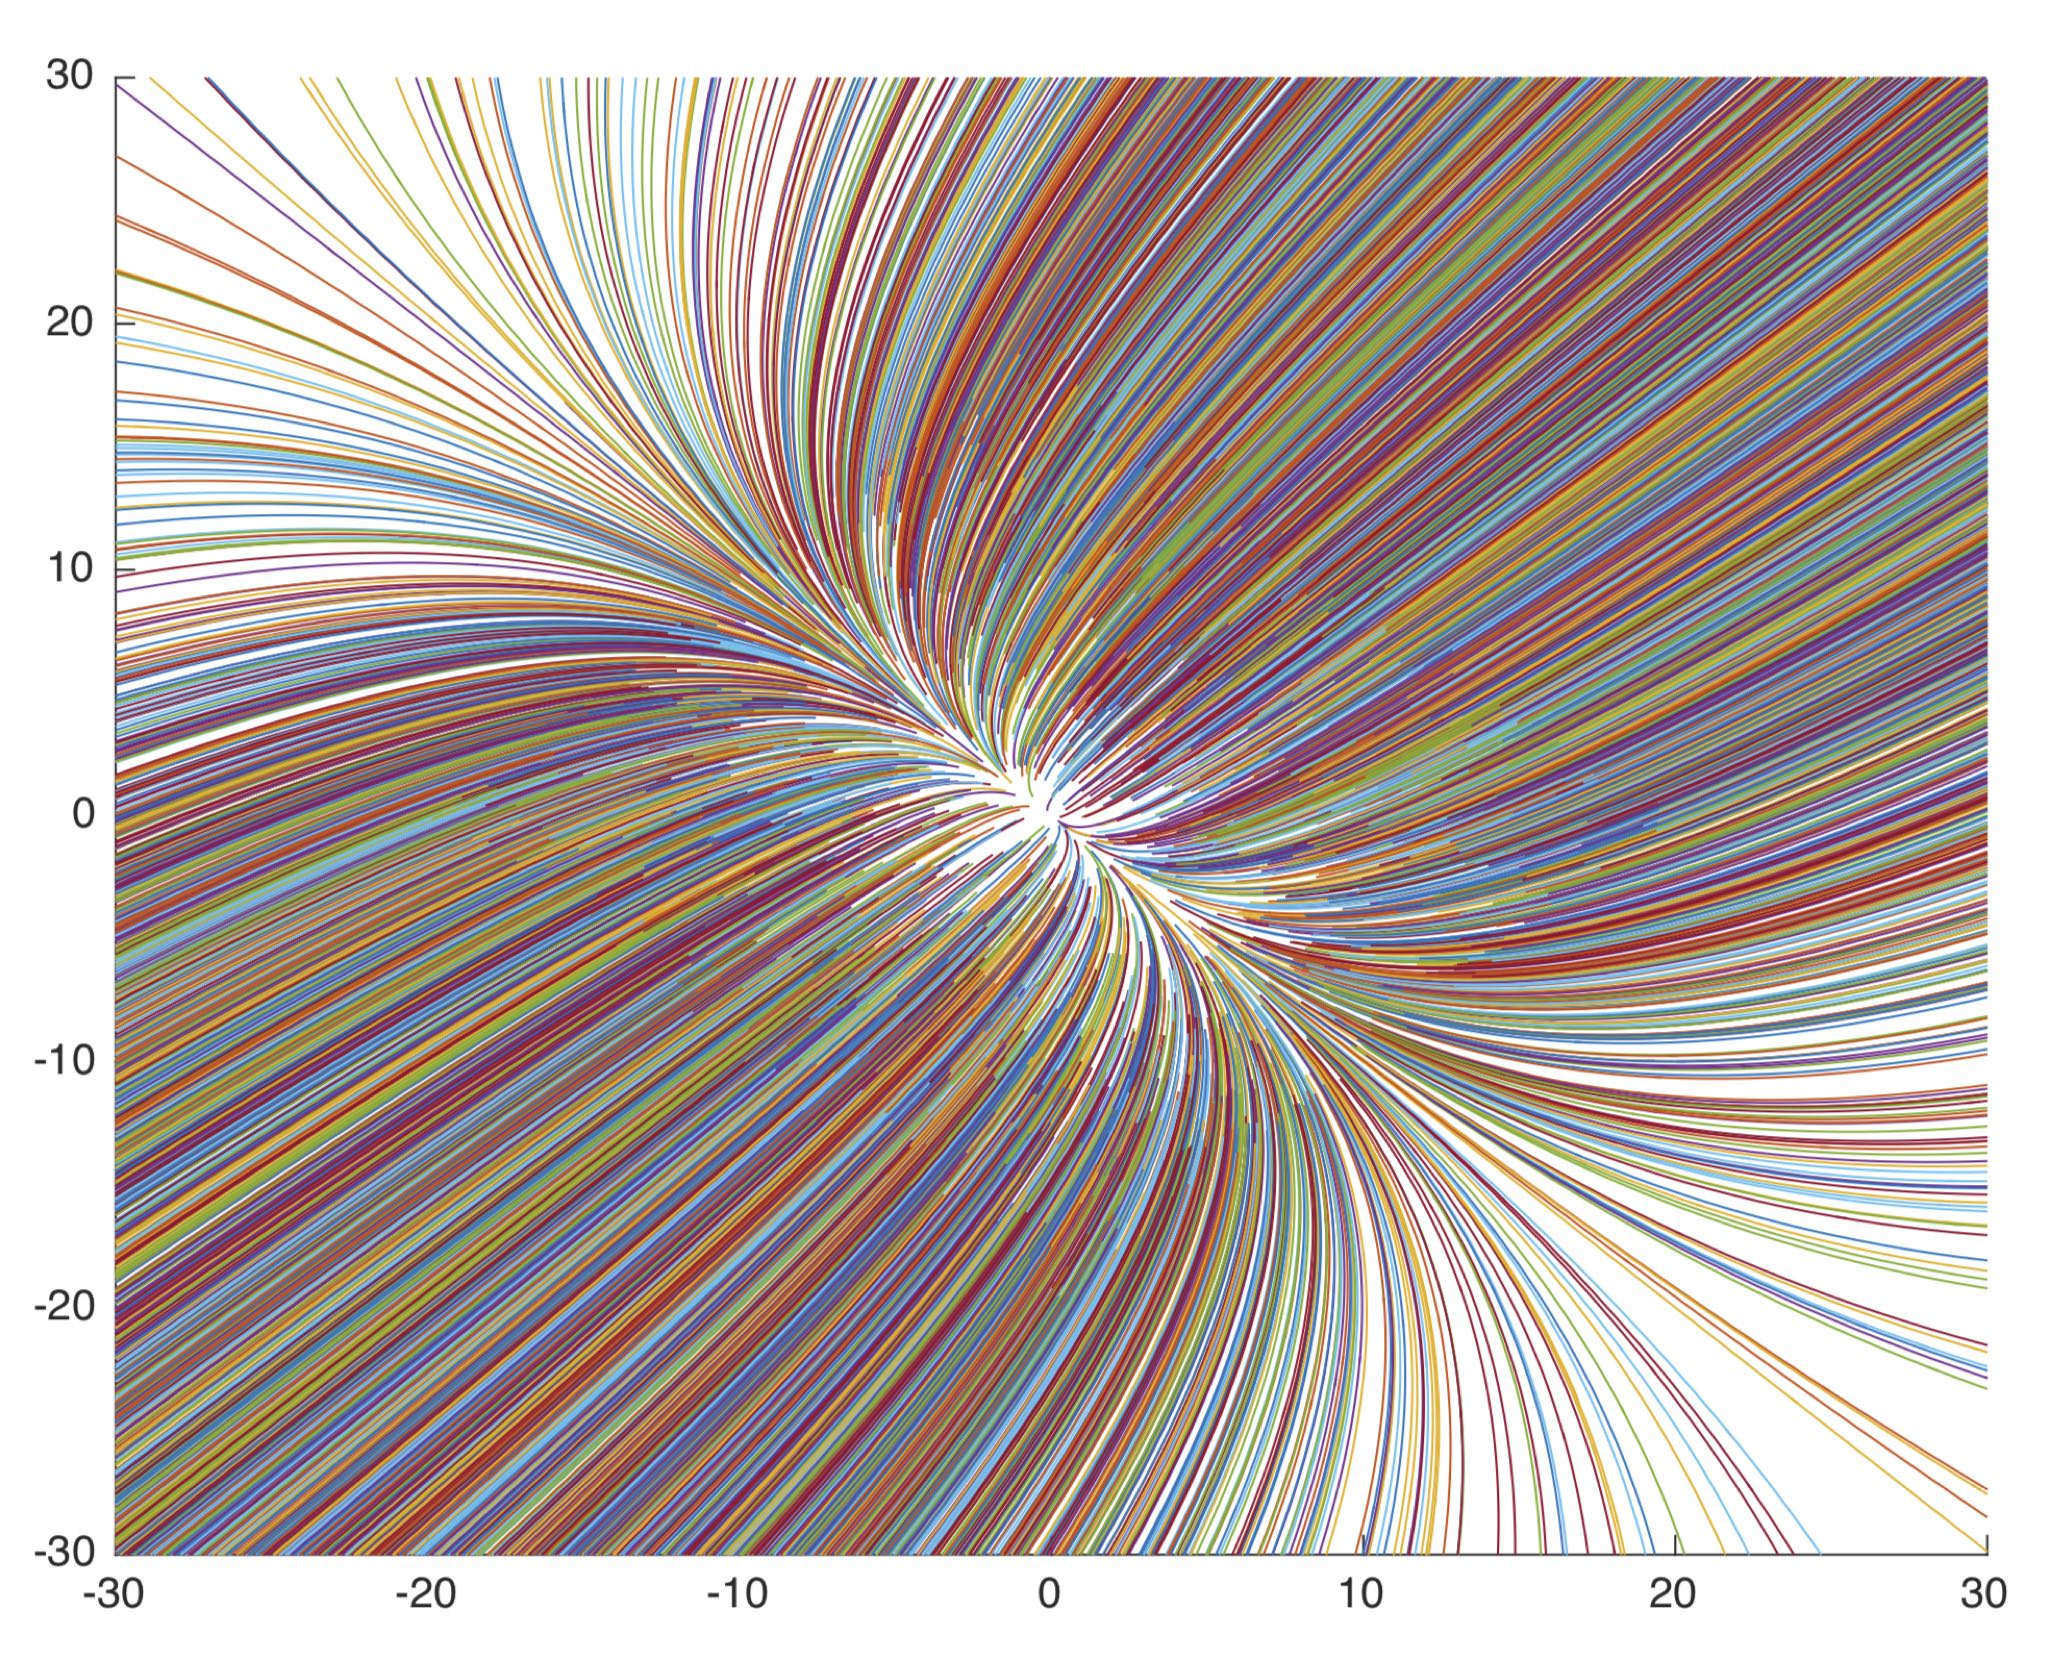
\includegraphics[scale=.1]{eks_1.jpg}
	\captionsetup{labelformat=empty}
	\caption{Eksempel \ref{eks_1}}
	\end{center}
\end{figure}


\begin{ex}
La 
\[
A=
-
\begin{bmatrix}
2 & 1  \\
1 & 2 
\end{bmatrix}
\]
slik at 
\[
\V y=
c_1
\begin{bmatrix}
1  \\
1 
\end{bmatrix} e^{-3t}
+
c_2
\begin{bmatrix}
1  \\
-1 
\end{bmatrix}e^{-t}. 
\]
Merk at uansett hvilke kombinasjoner av $c_1$ og $c_2$ vi har, så lenge ikke begge er 0, 
vil alle løsninger søke mot origo når $t\to \infty$, altså inn mot likevektsløsningen $\V y=0$. 
Vi sier derfor at $\V y$ er en \defterm{stabil likevektsløsning}.
\end{ex}

\begin{ex}
\label{eks_2}
La 
\[
A=
\begin{bmatrix}
1 & -2   \\
-2 & 1
\end{bmatrix}
\]
slik at 
\[
\V y=
c_1
\begin{bmatrix}
1  \\
1 
\end{bmatrix} e^{3t}
+
c_2
\begin{bmatrix}
1  \\
-1 
\end{bmatrix}e^{-t}. 
\]
Merk at så lenge $c_1 \neq 0$, 
vil alle løsninger gå mot uendelig når $t\to \infty$, altså inn mot likevektsløsningen $\V y=0$. 
Men dersom $c_1=0$ og $c_2\neq0$, vil løsningen søke mot origo. Likevektsløsningen $\V y=0$ kalles derfor en
\defterm{ustabil sadel}.
\end{ex}


\begin{figure}[htbp]
  \begin{center}
	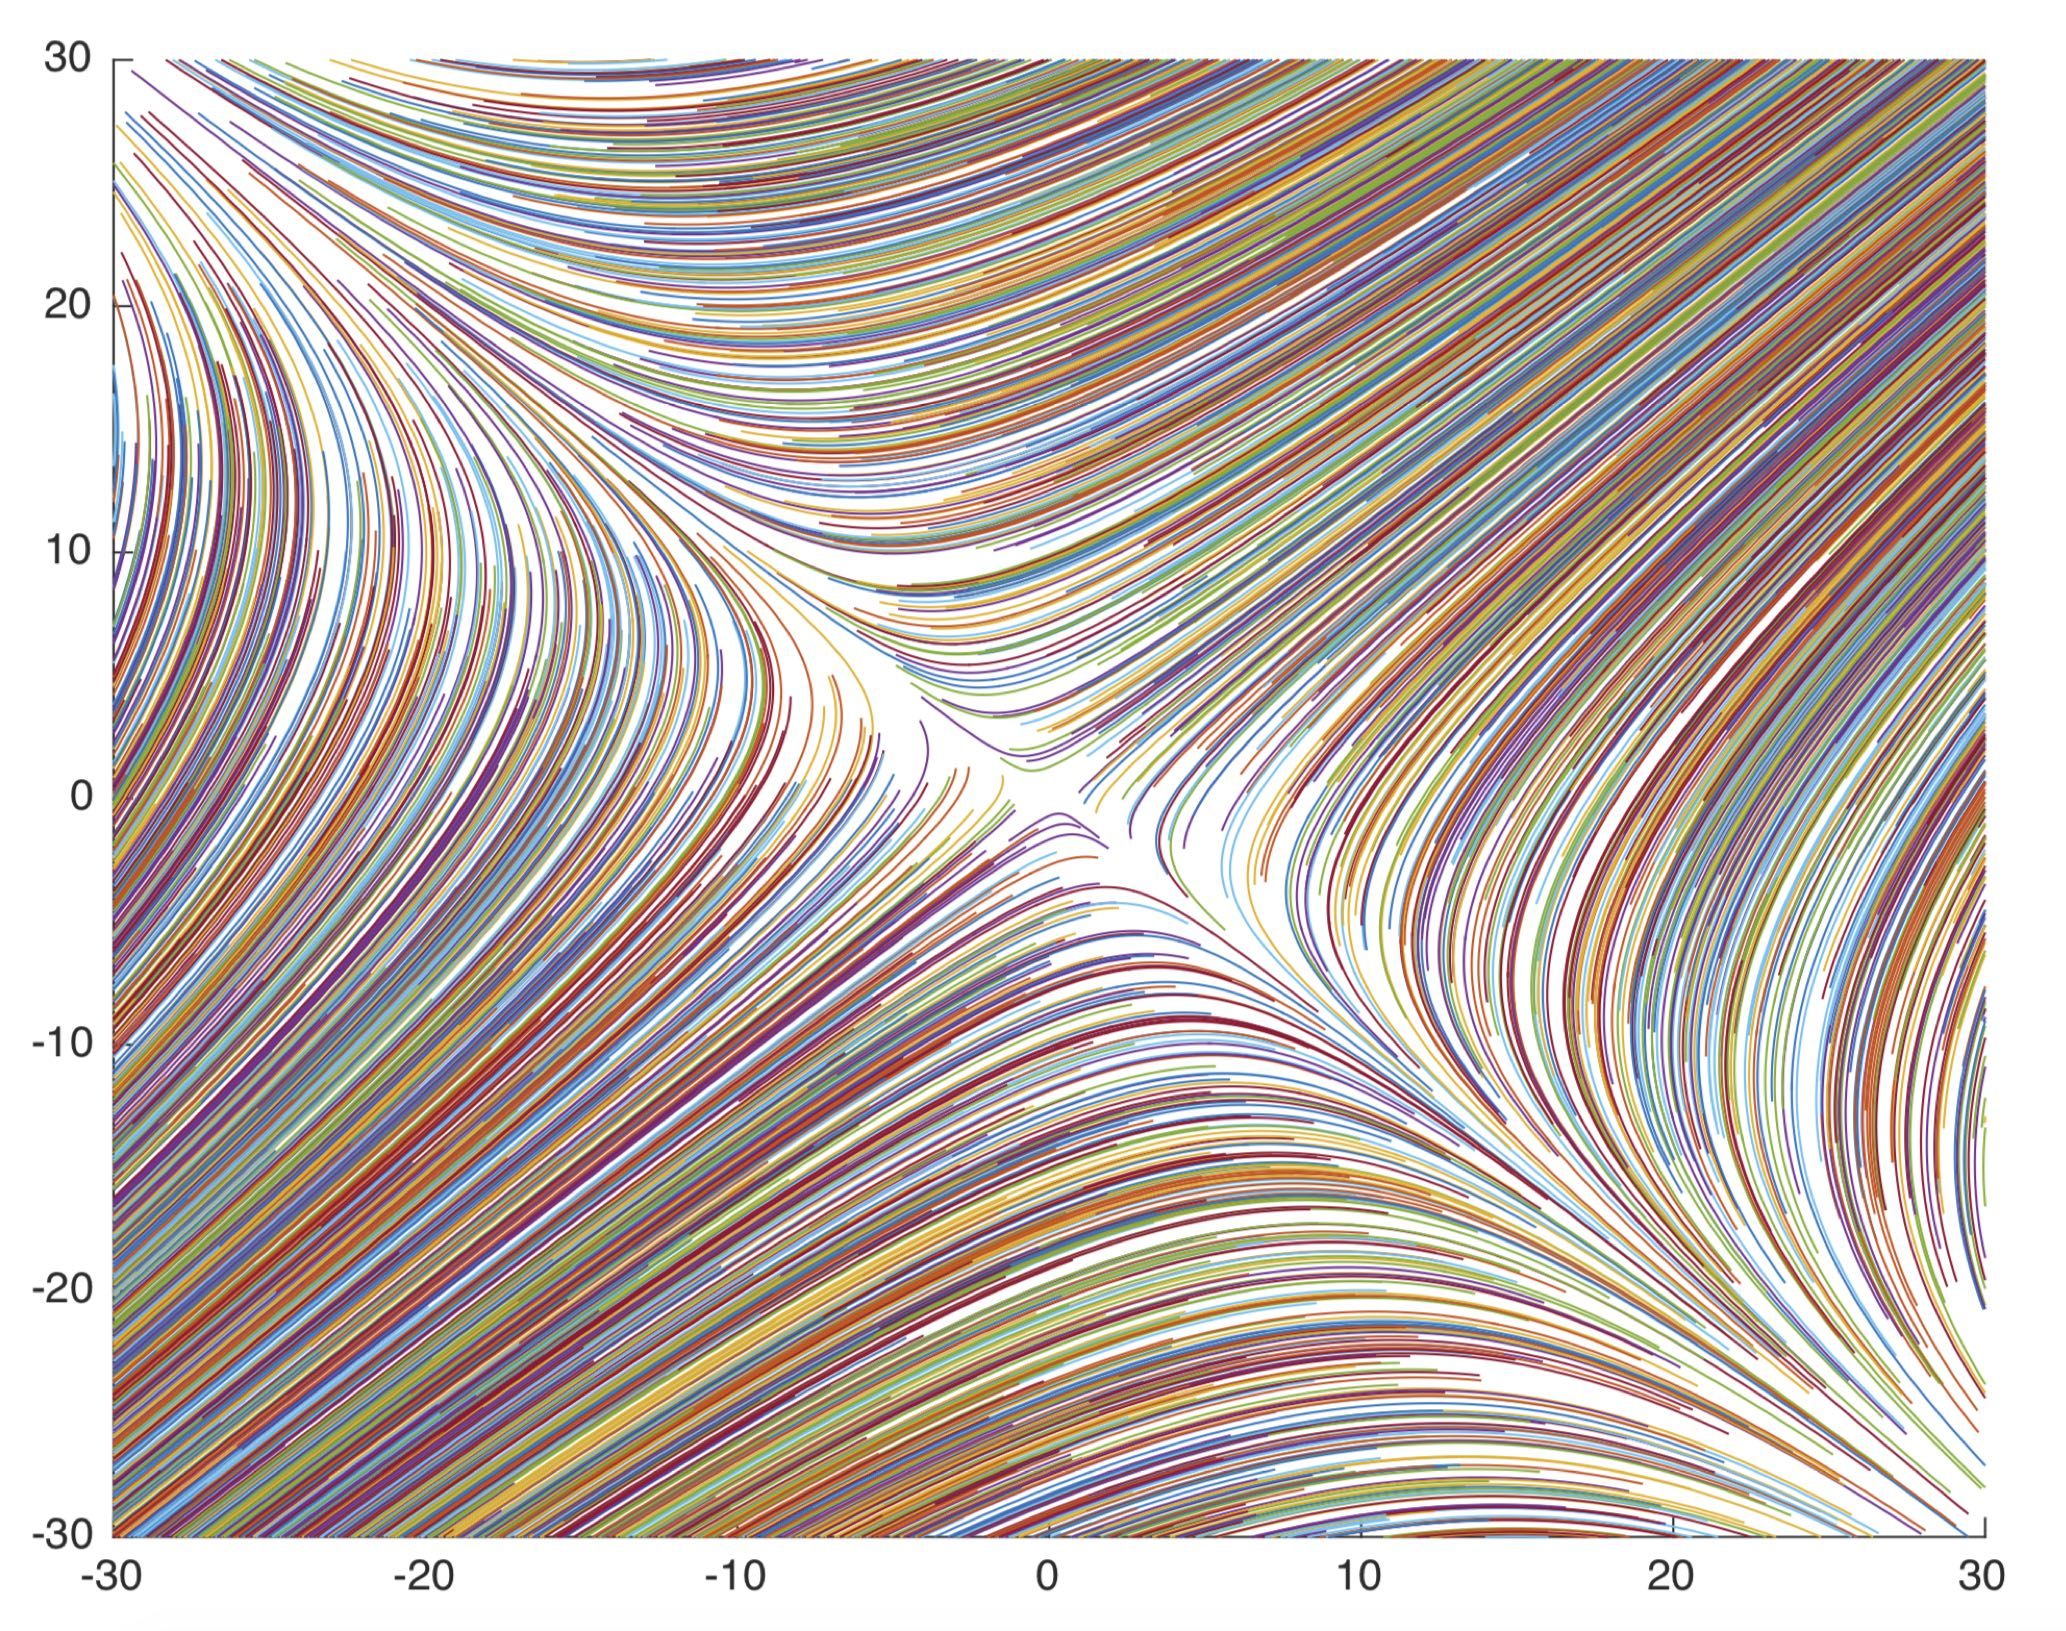
\includegraphics[scale=.1]{eks_2.jpg}	
	\captionsetup{labelformat=empty}
	\caption{Eksempel \ref{eks_2}}
	\end{center}
\end{figure}



\begin{ex}
La 
\[
A=-\frac{1}{2}
\begin{bmatrix}
3 & 3   \\
3 & 3
\end{bmatrix}
\]
slik at 
\[
\V y=
c_1
\begin{bmatrix}
1  \\
1 
\end{bmatrix} e^{-3t}
+
c_2
\begin{bmatrix}
1  \\
-1 
\end{bmatrix}. 
\]
Merk at så lenge $c_1 \neq 0$, 
vil alle løsninger søke mot likevektsløsningen
\[
\V y=
c_2
\begin{bmatrix}
1  \\
-1 
\end{bmatrix}. 
\]
og ingen mot $\V y=0$ når $t\to \infty$.
Dette er et eksempel på et problem som ikke er velformulert - ved å variere $t_0$ i startpunktet, 
kan vi lage løsningskurver som krysser hverandre, og dette går på tverke med entydigheten av løsninger.
\end{ex}



\subsubsection*{Komplekse egenverdier}
Vi har i øvingsopplegget vist at dersom en reell matrise har komplekse egenverdier, opptrer disse i komplekskonjugerte par.
Du har kanskje lagt merke til at dette også gjelder for de respektive egenvektorene:
\[
A\V x=\lambda \V x \quad \Longleftrightarrow \quad A \overline {\V x} =\overline{ \lambda} \overline {\V  x}
\]

Dette skal vi benytte oss av for å plukke ut relle løsninger. La $\lambda=\alpha+\beta i$ ha egenvektor 
\[\V x=\begin{bmatrix}  x_{1} \\ x_{2}\end{bmatrix}=\begin{bmatrix}  a_{1} \\ a_{2}\end{bmatrix}+i\begin{bmatrix}  b_{1} \\ b_{2}\end{bmatrix},\]
og husk at $e^{\alpha+\beta i}=e^{\alpha}(\cos \beta +i\sin{\beta})$, slik at
\begin{align*}
\V y(t)=\;&c_2\V y_1 +c_2\V y_2 \\ =\;&c_1e^{\lambda t}\V x +c_2e^{\overline{\lambda} t}\overline{\V x} \\ =\;&c_1e^{\alpha t}\left(\begin{bmatrix}  a_{1} \\ a_{2}\end{bmatrix}+i\begin{bmatrix}  b_{1} \\ b_{2}\end{bmatrix}\right)(\cos{\beta t}+i\sin{\beta t})\\+&c_2e^{\alpha t}\left(\begin{bmatrix}  a_{1} \\ a_{2}\end{bmatrix}-i\begin{bmatrix}  b_{1} \\ b_{2}\end{bmatrix}\right) (\cos{\beta t}-i\sin{\beta t}).
\end{align*}
Denne løsningen er pen på papiret, men vi ønsker å kunne visualisere litt, og da hadde det vært praktisk å finne en løsning som var reell istedet. 

Siden  $e^{\lambda t}\V x$ og $e^{\overline \lambda t}\overline{\V x}$ er lineært uavhengige for alle $t$, utgjør de en basis for $\C^2$. La oss søke en reell basis istedet.
Vi kaller den nye basisen $\V v_1$ og $\V v_2$. Velg først $c_1=c_2=\frac{1}{2}$, og sett
\[
\V v_1=e^{\alpha t} \left(\cos \beta t\begin{bmatrix}  a_{1} \\ a_{2}\end{bmatrix}-\sin \beta t\begin{bmatrix}  b_{1} \\ b_{2}\end{bmatrix}\right).
\]
Så velger vi $c_1=-c_2=\frac{1}{2i}$, og setter
\[
\V v_2=e^{\alpha t} \left(\cos \beta t\begin{bmatrix}  b_{1} \\ b_{2}\end{bmatrix}+\sin \beta t\begin{bmatrix}  a_{1} \\ a_{2}\end{bmatrix}\right).
\]
Nå kan vi skrive 
\begin{align*}
\V y(t)=\;&d_1\V v_1 +d_2\V v_2\\ =\;&d_1 e^{\alpha t} \left(\cos \beta t\begin{bmatrix}  a_{1} \\ a_{2}\end{bmatrix}-\sin \beta t\begin{bmatrix}  b_{1} \\ b_{2}\end{bmatrix}\right) 
\\+\;&d_2e^{\alpha t} \left(\cos \beta t\begin{bmatrix}  b_{1} \\ b_{2}\end{bmatrix}+\sin \beta t\begin{bmatrix}  a_{1} \\ a_{2}\end{bmatrix}\right). 
\end{align*}
Merk at siden $\V y_1$ og $\V y_2$ er lineært uavhengige, og forholdet mellom disse og $\V v_1$ og $\V v_2$ er gitt ved
\[
\begin{bmatrix} \V y_2  & \V y_2 \end{bmatrix}\begin{bmatrix} 1 & -i \\ 1 &i \end{bmatrix}=2\begin{bmatrix} \V v_2  & \V v_2 \end{bmatrix},
\]
er også $\V v_1$ og $\V v_2$ lineært uavhengige for alle $t$. Fordelen med den nye basisen er at vi nå enkelt kan skille ut alle reelle løsninger ved å holde oss til relle $d_1$ og $d_2$.


\begin{ex}
\label{eks_3}
La 
\[
A=
\begin{bmatrix}
0 & -1   \\
1 & 0
\end{bmatrix}
\]
som har egenverdier $\pm i$ og egenvektorer 
\[
\begin{bmatrix}
1  \\
i 
\end{bmatrix}
\quad \text{og} \quad
\begin{bmatrix}
1  \\
-i 
\end{bmatrix}. 
\]
Den generelle løsningen til systemet blir 
\begin{align*}
\V y(t)=\;&d_1 \left(\cos t\begin{bmatrix}  1 \\ 0\end{bmatrix}-\sin t\begin{bmatrix} 0 \\ 1\end{bmatrix}\right) 
\\+\;&d_2 \left(\cos t\begin{bmatrix} 0 \\ 1\end{bmatrix}+\sin t\begin{bmatrix}  1 \\ 0\end{bmatrix}\right)\\=\;&d_1\begin{bmatrix} \cos t \\ -\sin t\end{bmatrix}+d_2\begin{bmatrix}  \sin t \\ \cos t\end{bmatrix}=\begin{bmatrix} \cos t & \sin t\\ -\sin t & \cos t\end{bmatrix}\begin{bmatrix} d_1 \\ d_2 \end{bmatrix}.
\end{align*}
Vi ser at denne løsningen starter i punktet $\begin{bmatrix} d_1 \\ d_2 \end{bmatrix}$ ved $t=0$, og kjører deretter i en pen sirkulær bane om origo. 
Merk at kurven er traversert med klokken.
\end{ex}

\begin{figure}[htbp]
  \begin{center}
	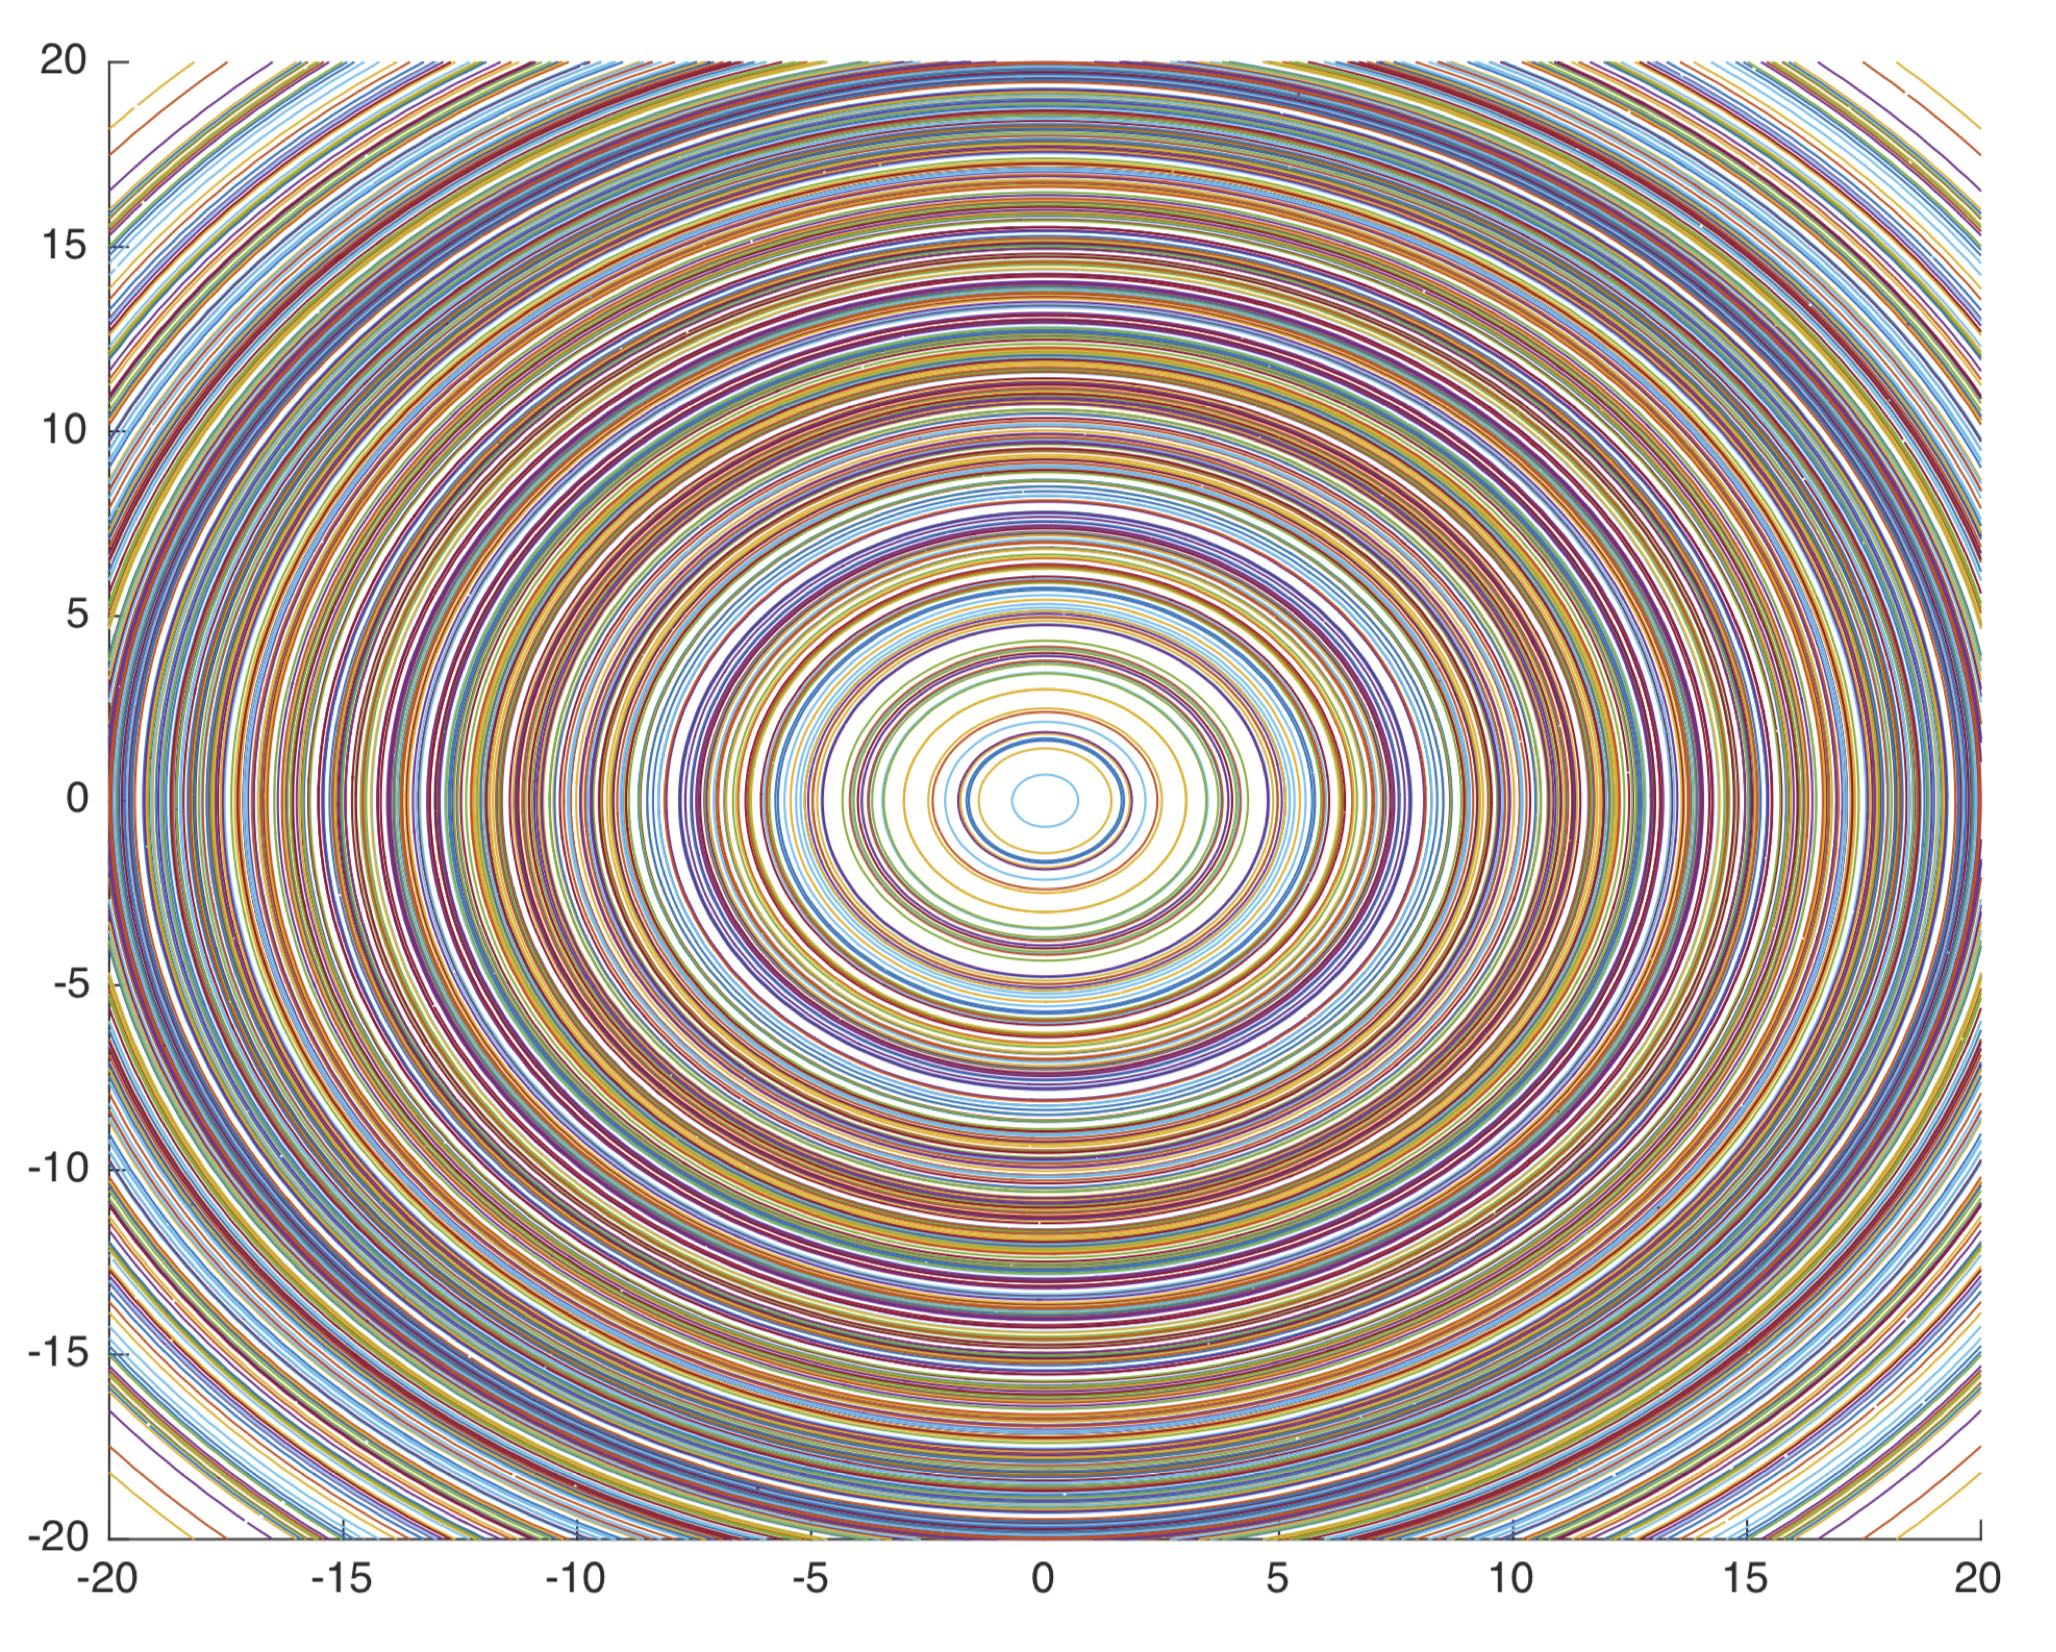
\includegraphics[scale=.1]{eks_3.jpg}
	\captionsetup{labelformat=empty}
	\caption{Eksempel \ref{eks_3}}
	\end{center}
\end{figure}



\begin{ex}
\label{eks_4}
La 
\[
A=
\begin{bmatrix}
1 & -1   \\
1 & 1
\end{bmatrix}
\]
som har egenverdier $1\pm i$ og de samme egenvektorene
\[
\begin{bmatrix}
1  \\
i 
\end{bmatrix}
\quad \text{og} \quad
\begin{bmatrix}
1  \\
-i 
\end{bmatrix}. 
\]
På samme vis som i forrige eksempel blir den generelle løsningen 
\begin{align*}
\V y(t)=\;&d_1e^t\begin{bmatrix} \cos t \\ -\sin t\end{bmatrix}+d_2e^t\begin{bmatrix}  \sin t \\ \cos t\end{bmatrix}\\&=\;e^t\begin{bmatrix} \cos t & \sin t\\ -\sin t & \cos t\end{bmatrix}\begin{bmatrix} d_1 \\ d_2 \end{bmatrix}.
\end{align*}
Denne løsningen starter i punktet $\begin{bmatrix} d_1 \\ d_2 \end{bmatrix}$ ved $t=0$, og kjører deretter i en særdeles vakker sirkulær og utadgående spiral.
\end{ex}


\begin{figure}[htbp]
  \begin{center}
	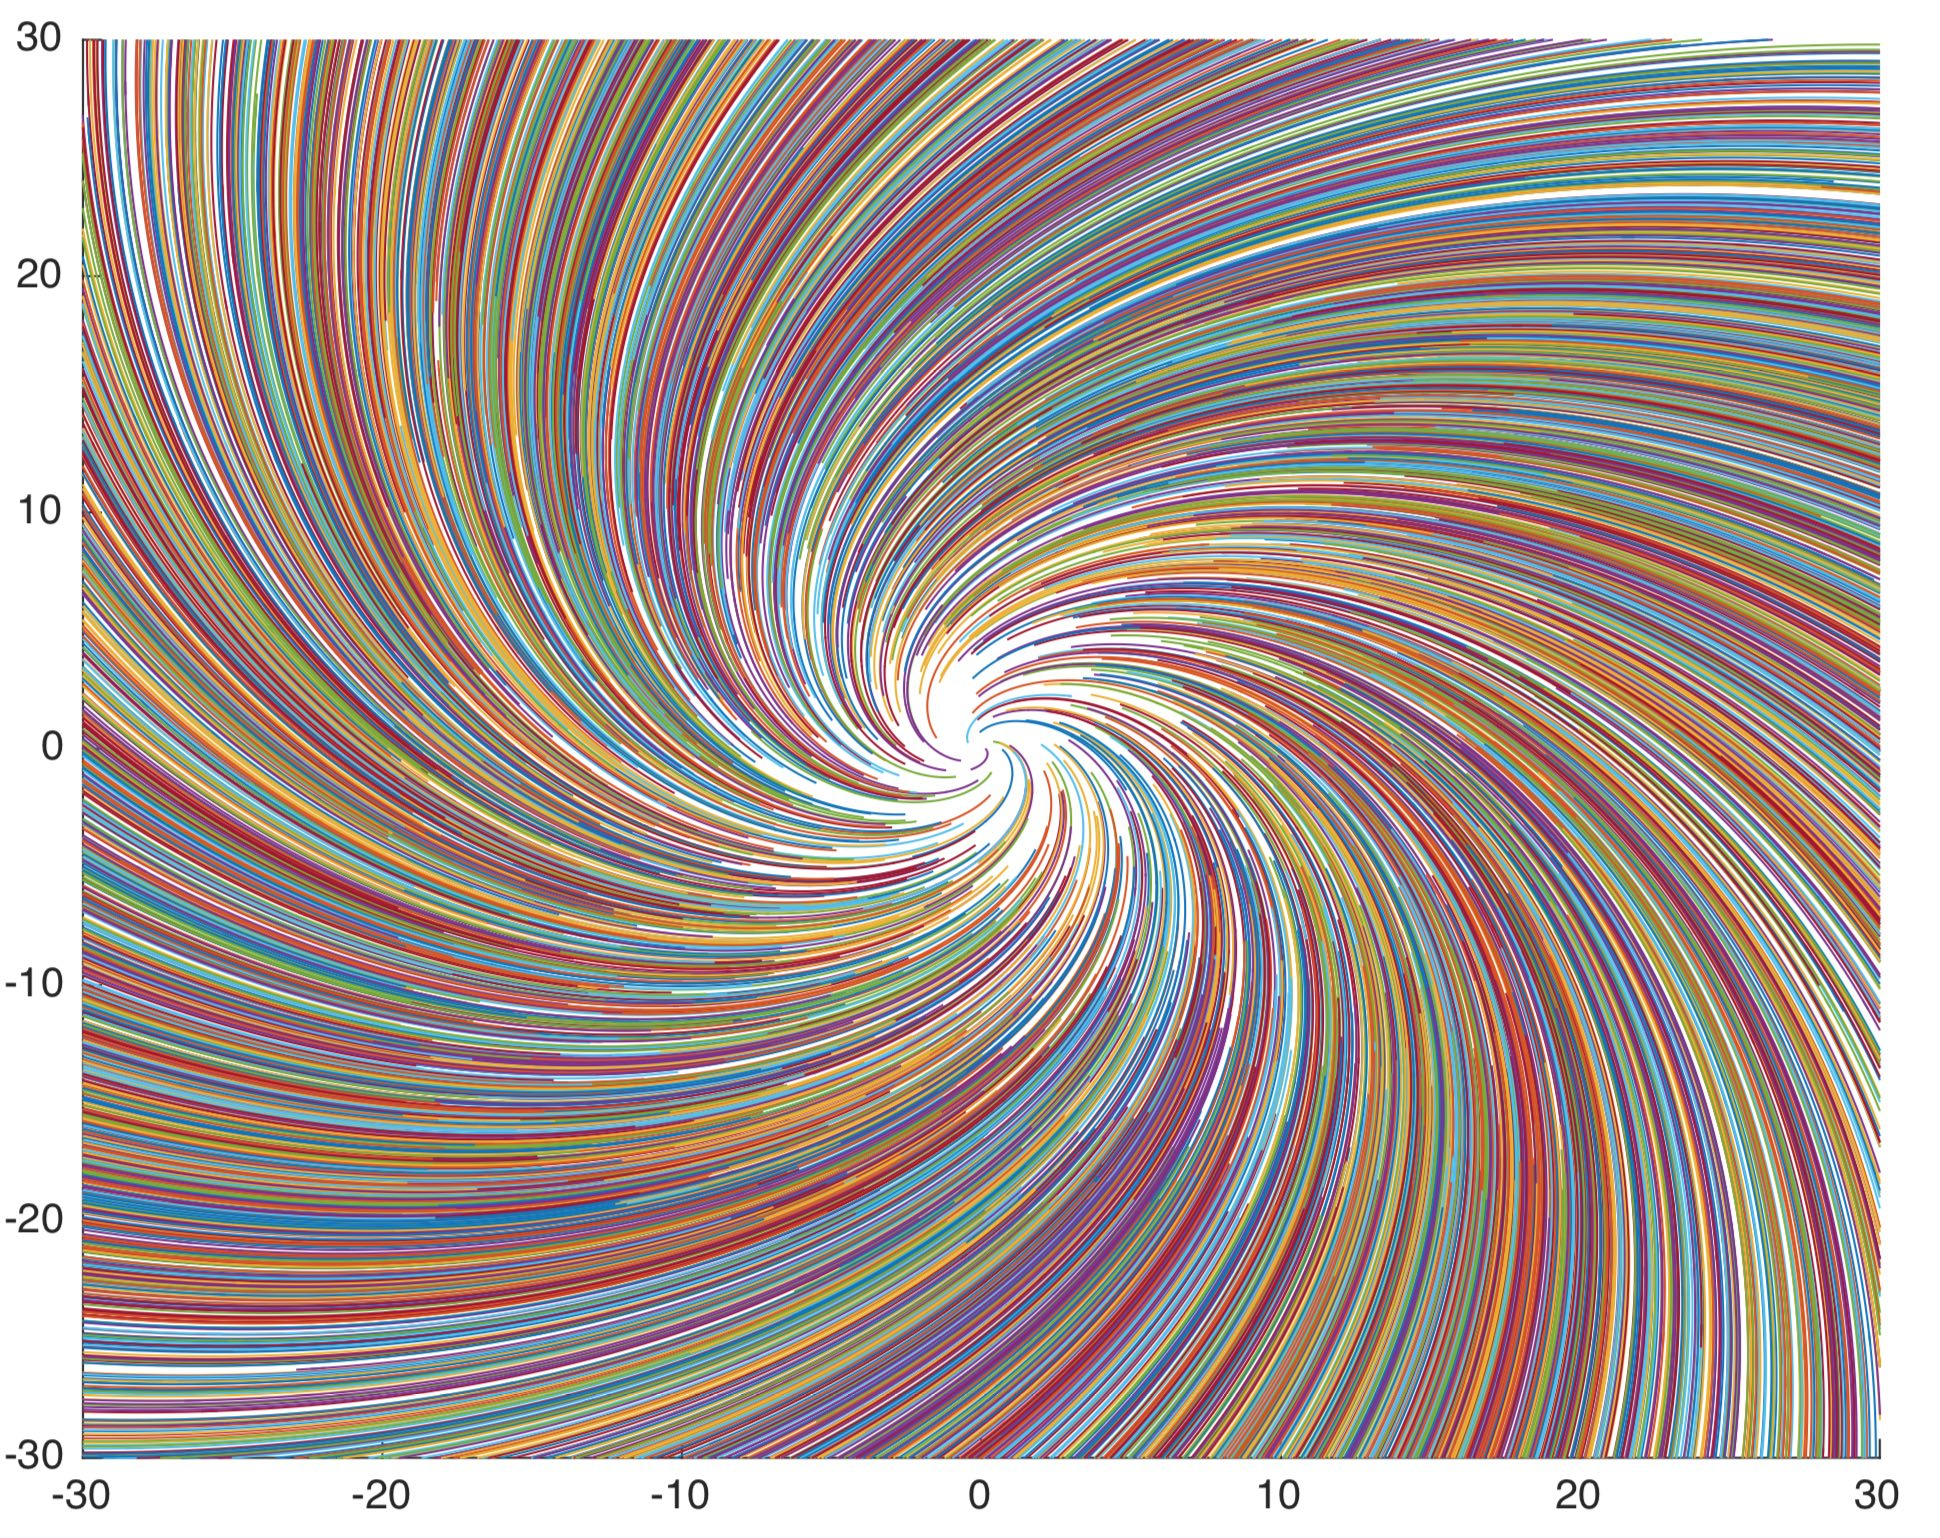
\includegraphics[scale=.1]{eks_4.jpg}
	\captionsetup{labelformat=empty}
	\caption{Eksempel \ref{eks_4}}
	\end{center}
\end{figure}



\begin{ex}
\label{eks_5}
La 
\[
A=
\begin{bmatrix}
-1 & -1   \\
1 & -1
\end{bmatrix}
\]
som har egenverdier $-1\pm i$ og de samme egenvektorene
\[
\begin{bmatrix}
1  \\
i 
\end{bmatrix}
\quad \text{og} \quad
\begin{bmatrix}
1  \\
-i 
\end{bmatrix}. 
\]
På samme vis som i de to forrige eksemplene blir den generelle løsningen 
\begin{align*}
\V y(t)=\;&d_1e^{-t}\begin{bmatrix} \cos t \\ -\sin t\end{bmatrix}+d_2e^{-t}\begin{bmatrix}  \sin t \\ \cos t\end{bmatrix}\\&=\;e^{-t}\begin{bmatrix} \cos t & \sin t\\ -\sin t & \cos t\end{bmatrix}\begin{bmatrix} d_1 \\ d_2 \end{bmatrix}.
\end{align*}
Denne løsningen starter i punktet $\begin{bmatrix} d_1 \\ d_2 \end{bmatrix}$ ved $t=0$, og kjører deretter i en innadgående sirkulær spiral.
\end{ex}


\begin{figure}[htbp]
  \begin{center}
	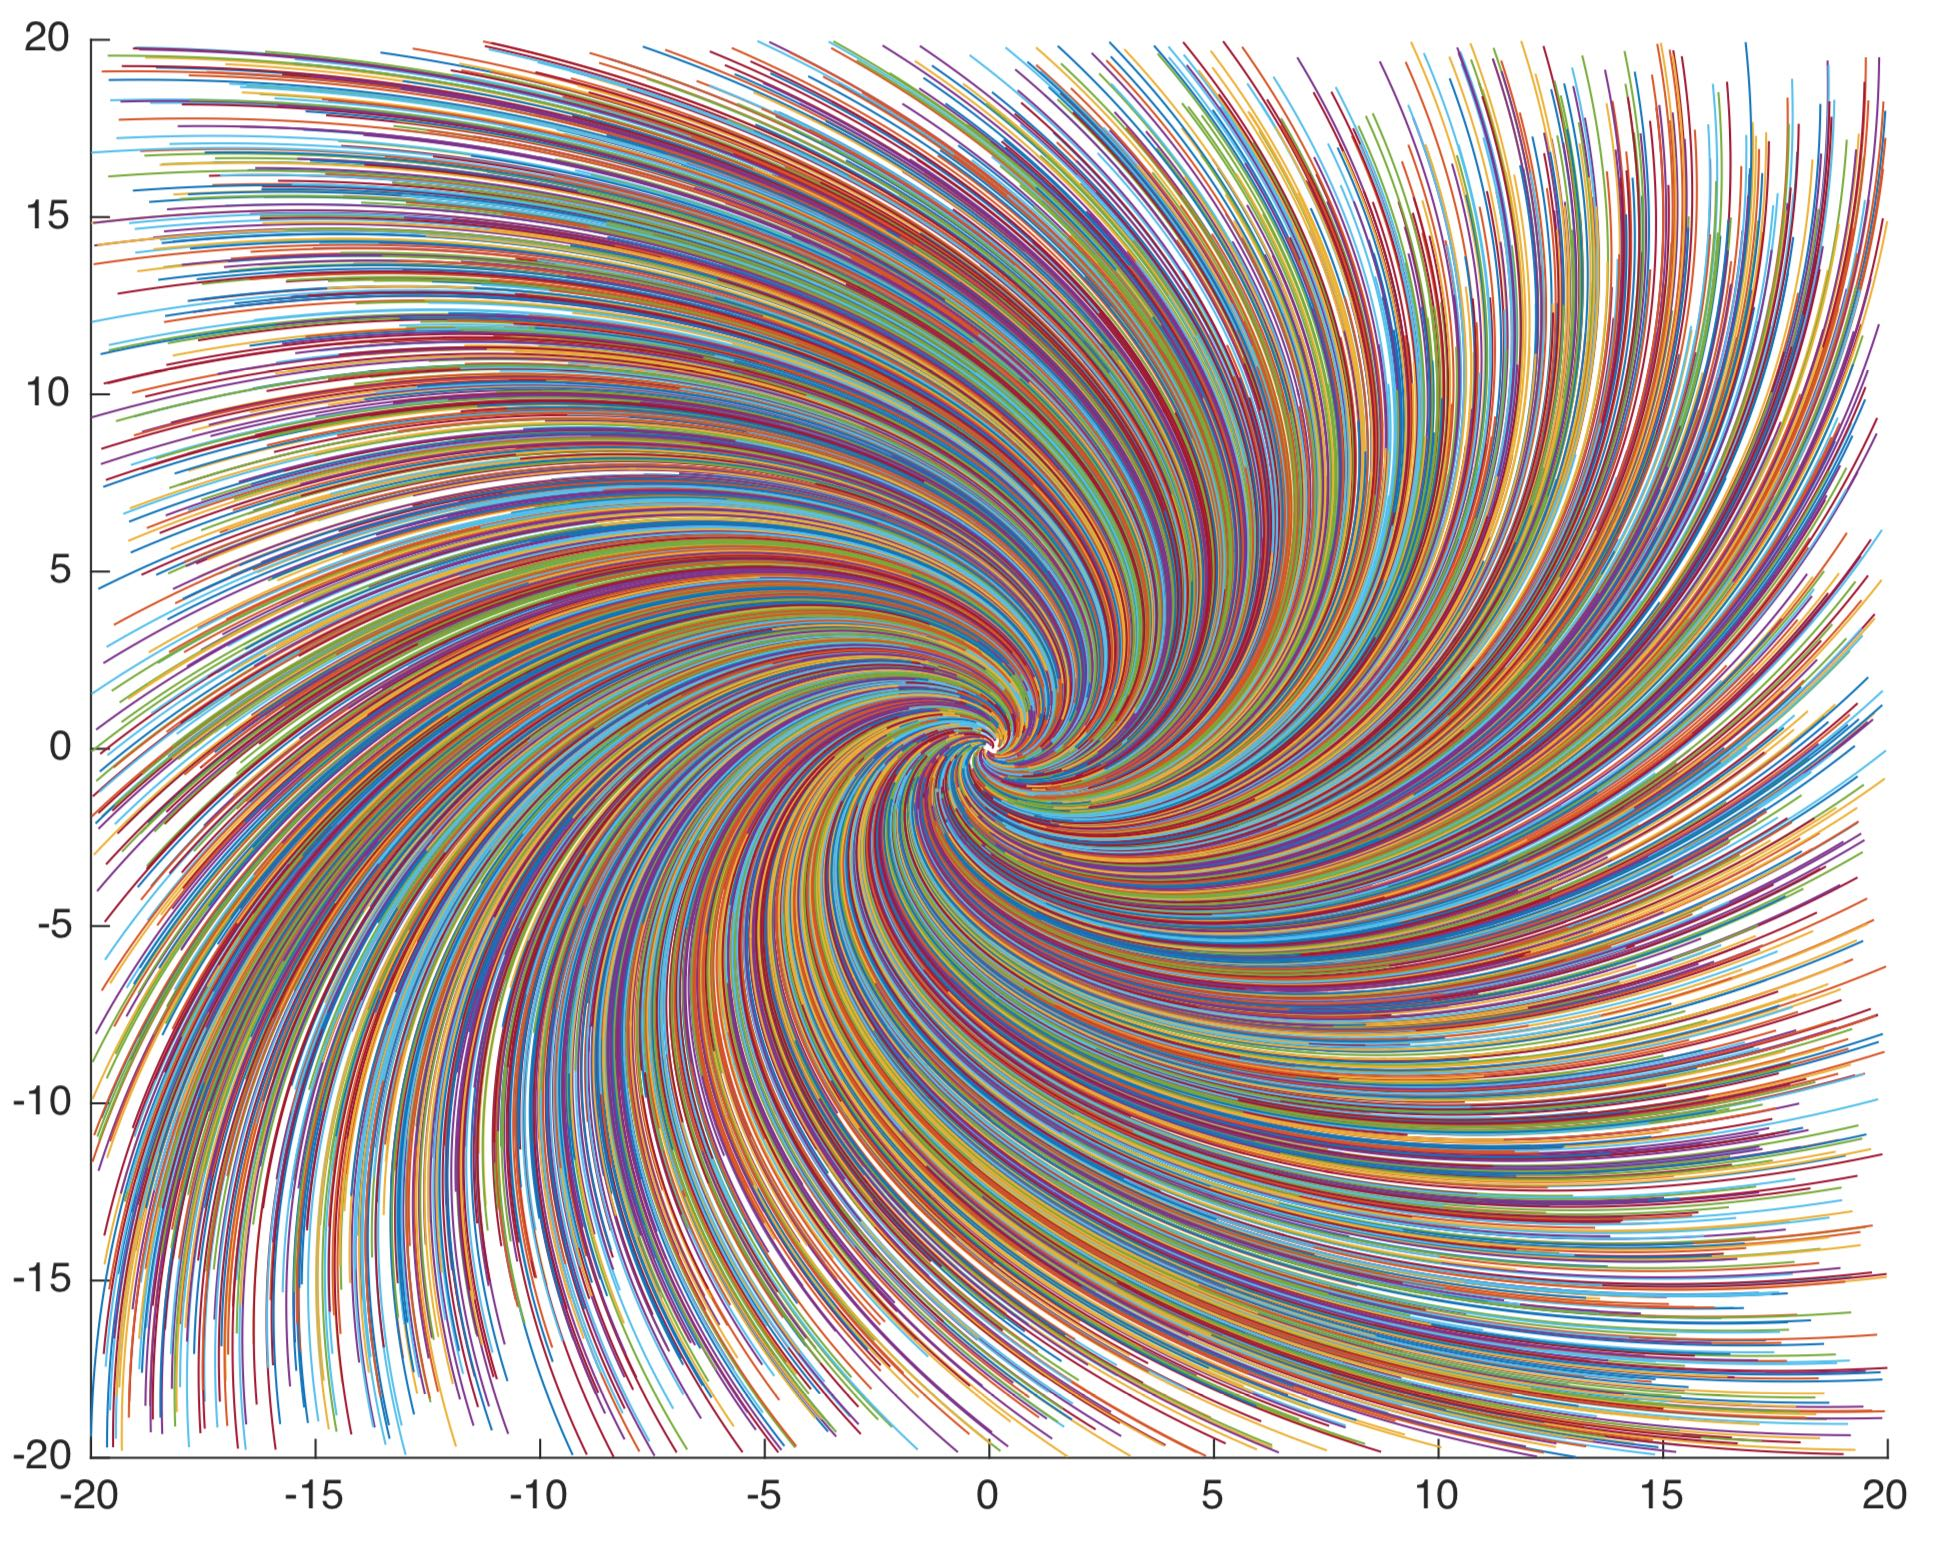
\includegraphics[scale=.1]{eks_5.jpg}
	\captionsetup{labelformat=empty}
	\caption{Eksempel \ref{eks_5}}
	\end{center}
\end{figure}
\subsubsection*{Dobbel egenverdi - for spesielt interesserte!}
Dette tilfellet kan vi egentlig ikke analysere med teorien vi har lært til nå, så du skal slippe å kunne det til eksamen. 
Men vi klarer ikke motstå fristelsen til å  bruke $2 \times 2$-matriser til å ta en smakebit på hva som skjuler seg utenfor pensum. 

\begin{ex}
La 
\[
A=
\begin{bmatrix}
0 & 1   \\
-1 & 2
\end{bmatrix}
\]
som har dobbel egenverdi $1$, men bare en egenvektor
$
\begin{bmatrix}
1  \\
1 
\end{bmatrix}
$.
Hva gjør vi nå?
\end{ex}

For å løse knipen fra forrige eksempel, må vi gjøre noe artig, nemlig introdusere \defterm{generalisert egenvektor}. 
Egenvektoren til $\lambda$ finner man ved å finne nullrommet til $A-\lambda I$. 
En generalisert egenvektor til en defekt egenverdi, finner man for $2 \times 2$-matriser ved å finne vektorer som er i nullrommet til $(A-\lambda I)^2$, 
men ikke i nullrommet til $A-\lambda I$.

\begin{ex}
La $A$ være som i forrige eksempel. Nullrommet til 
\[
(A-I)^2=
\left(\begin{bmatrix}
-1 & 1   \\
-1 & 1
\end{bmatrix}\right)^2=
\left(\begin{bmatrix}
0 & 0   \\
0 & 0
\end{bmatrix}\right)
\]
er jo alle vektorer i $\C^2$. Altså er alle vektorer i $\C^2$ unntatt vektorer som er parallelle med 
$
\begin{bmatrix}
1  \\
1 
\end{bmatrix},
$
generaliserte egenvektorer til matrisen $A$.
Vi velger oss en tilfeldig generalisert egenvektor til $A$, for eksempel
$
\begin{bmatrix}
-1  \\
1 
\end{bmatrix}.
$
Hvis vi ganger denne inn i $A-I$, får vi 
\[
\begin{bmatrix}
-1 & 1   \\
-1 & 1
\end{bmatrix}
\begin{bmatrix}
-1    \\
 1
\end{bmatrix}
=
\begin{bmatrix}
2    \\
2
\end{bmatrix},
\]
som er en egenvektor. Hm.
\end{ex}

Men hvordan bruker vi dette til å løse likningssystemet? 

\begin{ex}
Vektorene 
$
\begin{bmatrix}
-1  \\
1 
\end{bmatrix}
$
og 
$
\begin{bmatrix}
2  \\
2 
\end{bmatrix}
$
er et eksempel på en \defterm{kjede av generaliserte egenvektorer}. 
Løsningen som korresponderer til den genaliserte egenvektorkjeden 
$
\begin{bmatrix}
-1  \\
1 
\end{bmatrix}
$
og 
$
\begin{bmatrix}
2  \\
2 
\end{bmatrix}
$
er 
\[
\V y_2(t) = c_2 e^t
\left(
t
\begin{bmatrix}
2  \\
2 
\end{bmatrix}
+
\begin{bmatrix}
-1  \\
1 
\end{bmatrix}
\right).
\]
Løsningen som korresponderer til egenvektoren 
vi fant tidligere, er 
\[
\V y_1(t) = c_1 e^t
\begin{bmatrix}
1  \\
1 
\end{bmatrix}.
\]
Dette er to lineært uavhengige løsninger, og den generelle løsningen på systemet er 
\[
\V y(t) = c_1 e^t
\begin{bmatrix}
1  \\
1 
\end{bmatrix}
+ c_2 e^t
\left(
t
\begin{bmatrix}
2  \\
2 
\end{bmatrix}
+
\begin{bmatrix}
-1  \\
1 
\end{bmatrix}
\right).\qedhere
\]
\end{ex}

\kapittelslutt


% -*- TeX-master: "oving11"; -*-
\oppgaver{14}


\begin{oppgave}
Skissér faseplottet til systemet $A\V y=\V{y}'$ når
\begin{punkt}
$A= \begin{bmatrix}
2 & 3\\
-1 & -2
\end{bmatrix}
$	
\end{punkt}

\begin{punkt}
	$A= \begin{bmatrix}
	7 & -1\\
	3 & 3
	\end{bmatrix}
	$	
\end{punkt}

\begin{punkt}
	$A= \begin{bmatrix}
	-3 & 2\\
	-1 & -1
	\end{bmatrix}
	$	
\end{punkt}

\begin{punkt}
	$A= \begin{bmatrix}
	-3 & -9\\
	2 & 3
	\end{bmatrix}
	$	
\end{punkt}

\end{oppgave}


\begin{losning}
Vi ber kun om en skisse. Det holder å finne egenverdiene for å se hvordan systemet oppfører seg.
	\begin{punkt}
		Egenverdiene er $-1$ og~$1$, derfor får vi en sadel om origo.
	\end{punkt}
	
	\begin{punkt}
		Egenverdiene er $4$ og~$6$, derfor får vi en ustabilt likevektsløsning.
	\end{punkt}
	
	\begin{punkt}
		Egenverdiene er $2+i$ og~$2-i$, derfor får vi spiraler som er sirkulære og utgående fra origo.
	\end{punkt}
	
	\begin{punkt}
		Egenverdiene er $3i$ og~$-3i$, derfor får vi sirkulære baner om origo.
	\end{punkt}
	
\end{losning}


\begin{oppgave}
Finn generell løsning av $A\V y=\V y'$ når
\begin{punkt}
$
A=
\begin{bmatrix}
2 & 3 & 5\\
0 & 3 & 5\\
0 & 0 & 5
\end{bmatrix}
$ 
\end{punkt}
%
\begin{punkt}
$
A=
\begin{bmatrix}
3 & -1 & 2\\
3 & -1 & 6\\
-2 & 2 & -2
\end{bmatrix}$
\end{punkt}

\begin{punkt}
$
A=
\begin{bmatrix}
0 & -1 & 0\\
1 & 0 & 0\\
0 & 0 & 3
\end{bmatrix}$
\end{punkt}



\begin{punkt}
$
A=
\begin{bmatrix}
0 & -1 & 1& 5\\
1 & 0 & 2& 6\\
0 & 0 & 3 & 7\\
0 & 0 & 4 & 0
\end{bmatrix}$
\end{punkt}


\end{oppgave}

\begin{losning}
Du fant egenverdier og egenvektorer til alle matrisene i kapittel 13. Du trenger derfor bare å sette inn i formelen for generell løsning.


\begin{punkt}
	$$\V{y}=c_1\vvv{1}{0}{0}e^{2t}+c_2\vvv{3}{1}{0}e^{3t}+c_3\vvv{25}{15}{6}e^{5t}$$
\end{punkt}

\begin{punkt}
	$$\V{y}=c_1\vvv{1}{1}{0}e^{2t}+c_2\vvv{-2}{0}{1}e^{2t}+c_3\vvv{1}{3}{-1}e^{-4t}$$
\end{punkt}

\begin{punkt}
$$	\begin{aligned}
	\V{y}= {} & c_1\vvv{0}{0}{1}e^{3t}+c_2(\cos (t) \vvv{0}{1}{0}-\sin (t) \vvv{1}{0}{0})\\
	& +c_3(\cos (t) \vvv{1}{0}{0}+\sin (t) \vvv{0}{1}{0})
	\end{aligned}$$
	
\end{punkt}

\begin{punkt} 
$$	\begin{aligned}
	\V{y}= {} & c_1\vvvv{20}{12}{17}{-17}e^{-4t} +c_2\vvvv{151}{293}{350}{200}e^{7t}\\
	& +c_3(\cos (t) \vvvv{0}{1}{0}{0}-\sin (t) \vvvv{1}{0}{0}{0})\\
	& +c_4(\cos (t) \vvvv{1}{0}{0}{0}+\sin (t) \vvvv{0}{1}{0}{0})
	\end{aligned}$$

\end{punkt}


	
\end{losning}

\begin{oppgave}
Løs initialverdiproblemene $A\V y= \V y '$, $\V{y}(0)=\V{y}_0$ når 

\begin{punkt}
	$
	A=
	\begin{bmatrix}
	2 & 3 & 5\\
	0 & 3 & 5\\
	0 & 0 & 5
	\end{bmatrix}
	$, $
	\V{y}_0=\vvv{1}{0}{0}
	$
\end{punkt}
%
\begin{punkt}
	$
	A=
	\begin{bmatrix}
	3 & -1 & 2\\
	3 & -1 & 6\\
	-2 & 2 & -2
	\end{bmatrix}$, $
	\V{y}_0=\vvv{1}{-1}{1}
	$
\end{punkt}

\begin{punkt}
	$
	A=
	\begin{bmatrix}
	0 & -1 & 0\\
	1 & 0 & 0\\
	0 & 0 & 3
	\end{bmatrix}$, $
	\V{y}_0=\vvv{1}{2}{3}
	$
\end{punkt}


\end{oppgave}

\begin{losning}


\begin{punkt}
	$$\V{y}=\vvv{1}{0}{0}e^{2t}$$
\end{punkt}

\begin{punkt}
	$$\V{y}=2\vvv{1}{1}{0}e^{2t}-\vvv{1}{3}{-1}e^{-4t}$$
\end{punkt}

\begin{punkt}
	$$	\begin{aligned}
	\V{y}= {} & 3\vvv{0}{0}{1}e^{3t}+2(\cos (t) \vvv{0}{1}{0}-\sin (t) \vvv{1}{0}{0})\\
	& +(\cos (t) \vvv{1}{0}{0}+\sin (t) \vvv{0}{1}{0})
	\end{aligned}$$
	
\end{punkt}


	

\end{losning}

\begin{oppgave}
Løs initialverdiproblemet $$
A=
\begin{bmatrix}
0 & -1 & 0\\
1 & 0 & 0\\
0 & 0 & 3
\end{bmatrix}
\V{y}=\V{y}',\quad \V{y}(\frac{\pi}{2})=\vvv{1}{1}{1}.
$$
\end{oppgave}

\begin{losning}
	$$	\begin{aligned}
	\V{y}= {} & \vvv{0}{0}{1}e^{3(t-\frac{\pi}{2})}-(\cos (t) \vvv{0}{1}{0}-\sin (t) \vvv{1}{0}{0})\\
	& +(\cos (t) \vvv{1}{0}{0}+\sin (t) \vvv{0}{1}{0})
	\end{aligned}$$
\end{losning}


\begin{oppgave}
Vis at systemet
$$
\begin{bmatrix}
3 & -1 & 2\\
3 & -1 & 6\\
-2 & 2 & -2
\end{bmatrix} \V y= \V{y} '$$
med en gitt initialverdi $\V{y}(0)=\V{y}_0$ har en entydig løsning.\\

\noindent
\emph{Hint}: Du kan anta at den generelle løsningen inneholder alle løsninger.
\end{oppgave}

\begin{losning}
Vi har sett at den generelle løsningen er 
$$\V{y}=c_1\vvv{1}{1}{0}e^{2t}+c_2\vvv{-2}{0}{1}e^{2t}+c_3\vvv{1}{3}{-1}e^{-4t}.$$ Det gjenstår kun å bestemme koeffisientene fra initialverdiene:
$$c_1\vvv{1}{1}{0}+c_2\vvv{-2}{0}{1}+c_3\vvv{1}{3}{-1}=\V{y}_0.$$ Dette kan skrives som en matriseligning
$$\begin{bmatrix}
1 & -2 & 1\\
1 & 0 & 3\\
0 & 1 & -1
\end{bmatrix} \V c= \V{y}_0$$ hvor $\V c=\vvv{c_1}{c_2}{c_3}$. Du kan sjekke at kolonnene til denne matrisen er inverterbar. Dermed er det et entydig valg av koeffisienter $c_1$, $c_2$ og~$c_3$; løsningen er dermed entydig ettersom den generelle løsningen inneholder alle løsninger.
\end{losning}

\newpage
\begin{oppgave}\textbf{[Utfordring]}
	
\noindent
Husk at glatte funksjoner $f :\mathbb{R}\rightarrow \mathbb{R}$ er et vektorrom. På samme måte danner glatte vektorfunksjoner $\mathbf f:\mathbb{R}\rightarrow \mathbb{R}^n$ et vektorrom $V$ med addisjon
$$(\mathbf f + \mathbf g)(t)=\mathbf{f}(t)+\mathbf{g}(t),$$ og skalarmultiplikasjon
$$(c \mathbf f )(t)=c\mathbf{f}(t).$$

\begin{punkt}
Forklar hvorfor alle løsningene til et system $A\V y=\V{y}'$ danner et underrom av $V$.
\end{punkt}

\begin{punkt}
Hva er dimensjonen til rommet av alle løsninger til $$
\begin{bmatrix}
3 & -1 & 2\\
3 & -1 & 6\\
-2 & 2 & -2
\end{bmatrix} \V y= \V{y} ' ?$$

\noindent
\emph{Hint}: Bruk forrige oppgave.
\end{punkt}


\end{oppgave}





\begin{losning}
	\begin{punkt}
		Dette er superposisjonsprinsippet.
	\end{punkt}
	
	\begin{punkt}
	Vi viste i forrige oppgave at en løsning er entydig bestemt av en gitt initialverdi. Initialverdiene danner et tredimensjonalt rom. Derfor er dimensjonen lik tre.
	\end{punkt}
	
	
\end{losning}










\oppgaver{15}

\begin{oppgave}
Skriv om følgende andreordens differensiallikninger til system.

\begin{punkt}
$y''-y=0$
\end{punkt}

\begin{punkt}
	$y''+2y'+3y=0$
\end{punkt}

\begin{punkt}
	$y''+y'=0$
\end{punkt}


\end{oppgave}

\begin{losning} La $v=y'$.
	
	\begin{punkt}$\begin{bmatrix}
		0 & 1\\
		1 & 0
		\end{bmatrix} \vv{y}{v}=\vv{y}{v}'
		$
	\end{punkt}
	
	\begin{punkt}$\begin{bmatrix}
		0 & 1\\
		-3 & -2
		\end{bmatrix} \vv{y}{v}=\vv{y}{v}'
		$
	\end{punkt}
	
	\begin{punkt}$\begin{bmatrix}
		0 & 1\\
		0 & 1
		\end{bmatrix} \vv{y}{v}=\vv{y}{v}'
		$
	\end{punkt}
	
\end{losning}

\begin{oppgave}
Finn generell løsning av
\begin{punkt}
	$y''-y'-2y=0$
\end{punkt}

\begin{punkt}
	$y''+y=0$
\end{punkt}

\begin{punkt}
	$y''-4y'+4y=0$
\end{punkt}

\end{oppgave}

\begin{losning}
	\begin{punkt}
		$y=c_1 e^{2t}+c_2 e^{-t}$
	\end{punkt}
	
	\begin{punkt}
		$y=c_1\cos(t)+ c_2 \sin (t)$
	\end{punkt}
	
	\begin{punkt}
		$y=(c_1+tc_2)e^{2t}$
	\end{punkt}
	
\end{losning}


\begin{oppgave}
Løs initialverdiproblemet
	\begin{punkt}
		$y''-y'-2y=0$, $y(0)=0$, $y'(0)=1$
	\end{punkt}
	
	\begin{punkt}
		$y''+y=0$, $y(\frac{\pi}{2})=1$, $y'(\frac{\pi}{2})=0$
	\end{punkt}
	
	\begin{punkt}
		$y''-4y'+4y=0$, $y(1)=2$, $y'(0)=e^{-2}$
	\end{punkt}
	
\end{oppgave}

\begin{losning}
	\begin{punkt}
		$y=\frac{1}{3}( e^{2t}- e^{-t})$
	\end{punkt}
	
	\begin{punkt}
		$y= \sin (t)$
	\end{punkt}
	
	\begin{punkt}
		$y=(t-1)e^{2(t-1)}$
	\end{punkt}
	
\end{losning}


\begin{oppgave}
	Finn generell løsning av
	\begin{punkt}
		$y''-y'-2y=e^{-2t}$
	\end{punkt}

	\begin{punkt}
		$y''-y'-2y=e^{2t}$
	\end{punkt}
	
	\begin{punkt}
		$y''+y=t$
	\end{punkt}
	
	\begin{punkt}
		$y''-4y'+4y=4t$
	\end{punkt}
	
\end{oppgave}

\begin{losning}
	\begin{punkt} Prøv $y=a e^{-2t}$ for å finne
		$$y=c_1 e^{2t}+c_2 e^{-t}-\frac{1}{2}e^{-2t}.$$
	\end{punkt}

	\begin{punkt} Prøv $y=a t e^{2t}$ for å finne
		$$y=c_1 e^{2t}+c_2 e^{-t}+\frac{1}{3} t e^{2t}.$$
	\end{punkt}
	
	\begin{punkt} Prøv $a t$ for å finne
		$$y=c_1\cos(t)+ c_2 \sin (t)+t.$$
	\end{punkt}
	
	\begin{punkt} Prøv $at+b$ for å finne
		$$y=(c_1+tc_2)e^{2t}+t+1.$$
	\end{punkt}
	
\end{losning}

\begin{oppgave}
For alle ligningene i oppgave \textbf{15.1.} skal du: regne ut det karakteristiske polynomet til differensialligningen, og det karakteristiske polynomet til matrisen i tilhørende system. Ser du en sammenheng? Klarer du å bevise observasjonen din?
\end{oppgave}

\begin{losning}
Vi ser at polynomene blir like.
\\

Bevis: Betrakt en generell ligning $y''+py'+qy=0$. Det karakteristiske polynomet er $\lambda ^2+p\lambda+q$. Vi kan generelt skrive tilhørende system som $$\begin{bmatrix}
0 & 1\\
-q & -p
\end{bmatrix} \vv{y}{v}=\vv{y}{v} '
$$ hvor $v=y'$. Det karakteristiske polynomet til matrisen blir $$
\text{det}\begin{bmatrix}
-\lambda & 1\\
-q & -p-\lambda
\end{bmatrix}=\lambda(p+\lambda)+q=\lambda^2+p\lambda+q.
$$Polynomene er like.
\end{losning}

%\end{losning}
\ifx\inkludert\undefined
\documentclass[norsk,a4paper,twocolumn,oneside]{memoir}

\usepackage[utf8]{inputenc}
\usepackage{babel}
\usepackage{amsmath,amssymb,amsthm}
\usepackage[total={17cm,27cm}]{geometry}
\usepackage[table]{xcolor}
%\usepackage{tabularx}
\usepackage{systeme}
%\usepackage{hyperref}
%\usepackage{enumerate}

%\usepackage{sectsty}
\setsecheadstyle{\bfseries\large}
%\subsectionfont{\bf\normalsize}

\usepackage{tikz}
\usetikzlibrary{arrows.meta}

\newcommand{\defterm}[1]{\emph{#1}}

\newcommand{\N}{\mathbb{N}}
\newcommand{\Z}{\mathbb{Z}}
\newcommand{\Q}{\mathbb{Q}}
\newcommand{\R}{\mathbb{R}}

\newcommand{\abs}[1]{|#1|}

\newcommand{\roweq}{\sim}
\DeclareMathOperator{\Span}{Span}

\newcommand{\V}[1]{\mathbf{#1}}
\newcommand{\vv}[2]{\begin{bmatrix} #1 \\ #2 \end{bmatrix}}
\newcommand{\vvv}[3]{\begin{bmatrix} #1 \\ #2 \\ #3 \end{bmatrix}}
\newcommand{\vvvv}[4]{\begin{bmatrix} #1 \\ #2 \\ #3 \\ #4 \end{bmatrix}}
\newcommand{\vn}[2]{\vvvv{#1_1}{#1_2}{\vdots}{#1_#2}}

\newenvironment{amatrix}[1]{% "augmented matrix"
  \left[\begin{array}{*{#1}{c}|c}
}{%
  \end{array}\right]
}

% \newcounter{notatnr}
% \newcommand{\notatnr}[2]
% {\setcounter{notatnr}{#1}%
%  \setcounter{page}{#2}%
% }

\newtheorem{thm}{Teorem}[chapter]
\newtheorem*{thm-nn}{Teorem}
\newtheorem{cor}[thm]{Korollar}
\newtheorem{lem}[thm]{Lemma}
\newtheorem{prop}[thm]{Proposisjon}
\theoremstyle{definition}
\newtheorem{exx}[thm]{Eksempel}
\newtheorem*{defnx}{Definisjon}
\newtheorem*{oppg}{Oppgave}
\newtheorem*{merkx}{Merk}
\newtheorem*{spmx}{Spørsmål}

\newenvironment{defn}
  {\pushQED{\qed}\renewcommand{\qedsymbol}{$\triangle$}\defnx}
  {\popQED\enddefnx}
\newenvironment{ex}
  {\pushQED{\qed}\renewcommand{\qedsymbol}{$\triangle$}\exx}
  {\popQED\endexx}
\newenvironment{merk}
  {\pushQED{\qed}\renewcommand{\qedsymbol}{$\triangle$}\merkx}
  {\popQED\endmerkx}
\newenvironment{spm}
  {\pushQED{\qed}\renewcommand{\qedsymbol}{$\triangle$}\spmx}
  {\popQED\endspmx}

\setlength{\columnsep}{26pt}

\newcommand{\Tittel}[2]{%
\twocolumn[
\begin{center}
\Large
\begin{tabularx}{\textwidth}{cXr}
\cellcolor{black}\color{white}%
\bf {#1} &
#2
\hfill &
\footnotesize TMA4110 høsten 2018
\\ \hline
\end{tabularx}
\end{center}
]}

\newcommand{\tittel}[1]{\Tittel{\arabic{notatnr}}{#1}}

\newcommand{\linje}{%
\begin{center}
\rule{.8\linewidth}{0.4pt}
\end{center}
}


\newcommand{\chapternumber}{}

\makechapterstyle{tma4110}{%
 \renewcommand*{\chapterheadstart}{}
 \renewcommand*{\printchaptername}{}
 \renewcommand*{\chapternamenum}{}
 \renewcommand*{\printchapternum}{\renewcommand{\chapternumber}{\thechapter}}
 \renewcommand*{\afterchapternum}{}
 \renewcommand*{\printchapternonum}{\renewcommand{\chapternumber}{}}
 \renewcommand*{\printchaptertitle}[1]{
\LARGE
\begin{tabularx}{\textwidth}{cXr}
\cellcolor{black}\color{white}%
\textbf{\chapternumber} &
\textbf{##1}
\hfill &
%\footnotesize TMA4110 høsten 2018
\\ \hline
\end{tabularx}%
}
 \renewcommand*{\afterchaptertitle}{\par\nobreak\vskip \afterchapskip}
 % \newcommand{\chapnamefont}{\normalfont\huge\bfseries}
 % \newcommand{\chapnumfont}{\normalfont\huge\bfseries}
 % \newcommand{\chaptitlefont}{\normalfont\Huge\bfseries}
 \setlength{\beforechapskip}{0pt}
 \setlength{\midchapskip}{0pt}
 \setlength{\afterchapskip}{10pt}
}


\newcounter{oppgnr}[chapter]
\newcounter{punktnr}[oppgnr]
\newenvironment{oppgave}
 {\par\noindent\stepcounter{oppgnr}\textbf{{\arabic{oppgnr}}.}}
 {\par\bigskip}
\newenvironment{punkt}
 {\par\smallskip\noindent\stepcounter{punktnr}\textbf{\alph{punktnr})} }
 {\par}

\newcommand{\oppgaver}{\linje\section*{Oppgaver}}

\usepackage{xr}
\externaldocument{tma4110-2018h}
\newcommand{\kapittel}[2]{\setcounter{chapter}{#1}\addtocounter{chapter}{-1}\chapter{#2}}
\newcommand{\kapittelslutt}{\enddocument}
\begin{document}
\chapterstyle{tma4110}
\pagestyle{plain}
\fi


\kapittel{15}{Andre ordens lineære differensiallikninger}
\label{ch:andre-ordens-lineare-differensiallikninger}


I matte 1 har du løst to typer differensiallikninger. Den ene er den første ordens lineære likningen
\[
y'+f(t)y=g(t)
\]
og den andre er den separable likningen
\[
y'=f(y)g(t).
\]
I dette avsnittet skal vi behandle lineære andreordens differensiallikninger med konstante koeffisienter:
\[
y''+a_1y'+a_0y=0
\]
Det er vanlig å kreve at $y \in \mathcal C^2$, altså at $y$ har to kontinuerlige deriverte. 
På denne måten kan man sikre at likningen faktisk gir mening. 
Det finnes mange situasjoner der dette kravet kan slakkes noe, 
men det er pensum i matte 4.  

%Vi skal behandle den andre ordens differensiallikningen ved å skrive den om til et system 
%Dersom $f=0$, kalles likningen \defterm{homogen}. 
%Siden $L$ er en lineærtransformasjon, 
%kan vi umiddelbart dedusere at dersom to funksjoner er løser en homogen likning, 
%vil også lineærkombinasjoner av dem gjøre det. 
%Dette kalles \defterm{superposisjonsprinsippet}.






\section*{Hvor kommer andre ordens differensiallikninger fra?}
En kloss sklir friksjonsfritt p{\aa} underlaget, og er festet til veggen med en fj{\ae}r. Hookes fj{\ae}rlov sier at 
\begin{figure}[htbp]
  \begin{center}
	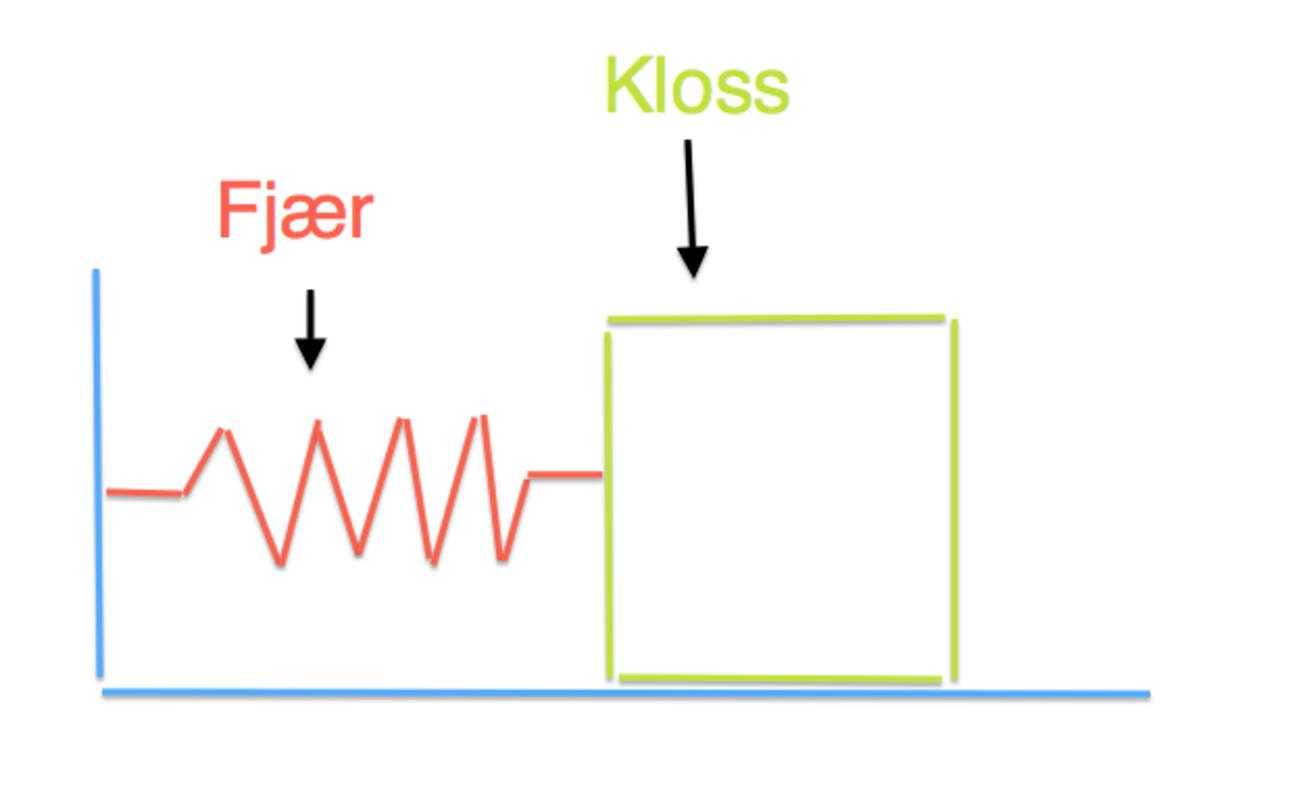
\includegraphics[scale=.35]{Hooke.pdf}
	\label{fig:Num1}
	\end{center}
\end{figure}
\[
F(x)=-kx,
\]
der $x$ er hvor langt fj{\ae}ren er strukket eller komprimert, 
$k$ er en konstant som avhenger av fj{\ae}rens stivhet, 
og $F(x)$ er kraften fra fj{\ae}ren p{\aa} klossen. 
Dersom $x(t)$ er klossens posisjon, er klossens akselerasjon gitt ved $x''(t)$,
og Newtons andre lov blir
\begin{equation*}
-kx=mx'',
\end{equation*}
der $m$ er klossens masse. Dette er en differensiallikning. Vi skriver vanligvis
\[
mx''+kx=0.
\]

Vi kan komplisere det litt til. La oss innf{\o}re luftmotstand. Luftmotstand avhenger kvadratisk av farten:
\begin{equation*}
F(x')=b(x')^{2};
\end{equation*}
der $b$ er en proporsjonalitetskonstant som sier noe om luftmotstanden. 
Den totale kraften blir
\begin{equation*}
F(x,x')=-kx+b(x')^{2},
\end{equation*}
slik at Newtons andre lov gir
\begin{equation*}
mx''-b(x')^{2} +kx=0.
\end{equation*}
Denne likningen har et problematisk ledd, $b(x')^{2}$. Men vi kan gjøre en forenkling. 
Dersom klossen ligger i en tyktflytende væske, blir motstanden proporsjonal med farten istedet for kvadratet av farten, 
og vi får likningen
\begin{equation*}
mx''-cx' +kx=0,
\end{equation*}
som er mye enklere å løse.



N{\aa} skal vi komplisere det enda litt. La klossen henge fra taket.
\begin{figure}[htbp]
  \begin{center}
	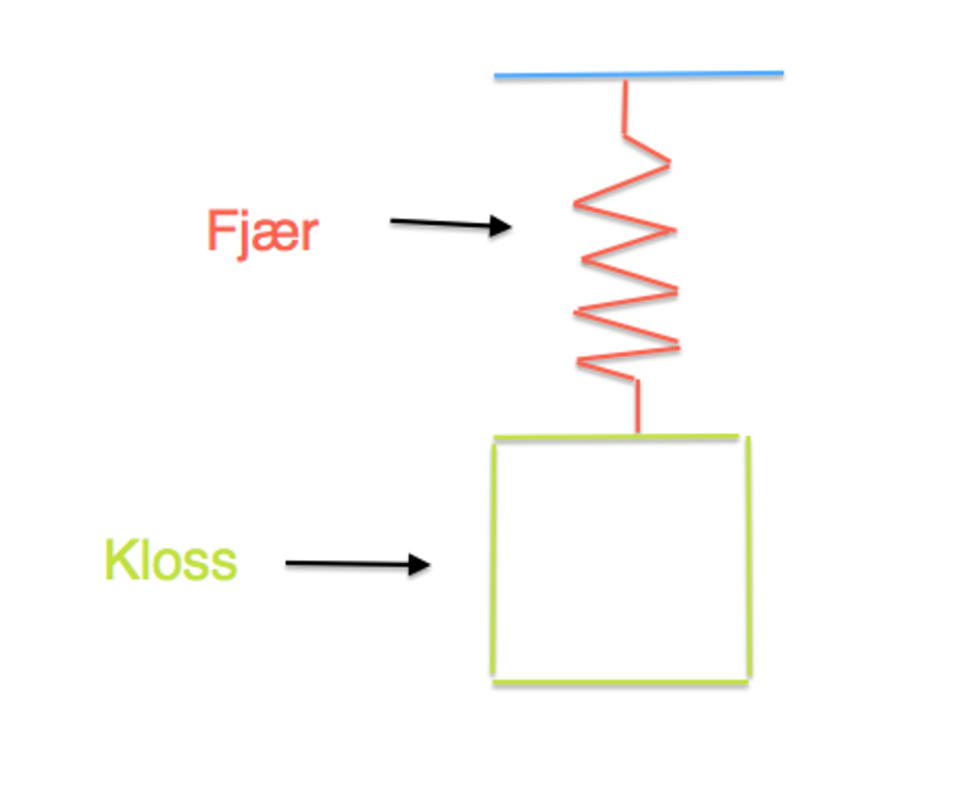
\includegraphics[scale=.4]{Hooke_2.pdf}
	\label{fig:Num1}
	\end{center}
\end{figure}
I tillegg til fj{\ae}rkraften og luftmotstanden, vil n{\aa} ogs{\aa} gravitasjonen p{\aa}virke bevegelsen. Gravitasjonskraften er en konstant kraft $mg$ nedover. Den totale kraften
er
\begin{equation*}
F(x,x')=-kx+bx'-mg,
\end{equation*}
og Newtons andre lov gir differensiallikningen
\begin{equation*}
mx''-bx' +kx=mg.
\end{equation*}





\section*{Omskrivning til system}
En annen ordens differensialikning kan skrives om til et system 
\kapittelslutt

%\oppgaver{15}

\begin{oppgave}
Skriv om følgende andre ordens differensiallikninger til system.

\begin{punkt}
$y''-y=0$
\end{punkt}

\begin{punkt}
	$y''+2y'+3y=0$
\end{punkt}

\begin{punkt}
	$y''+y'=0$
\end{punkt}


\end{oppgave}

\begin{losning} La $v=y'$.
	
	\begin{punkt}$\begin{bmatrix}
		0 & 1\\
		1 & 0
		\end{bmatrix} \vv{y}{v}=\vv{y}{v}'
		$
	\end{punkt}
	
	\begin{punkt}$\begin{bmatrix}
		0 & 1\\
		-3 & -2
		\end{bmatrix} \vv{y}{v}=\vv{y}{v}'
		$
	\end{punkt}
	
	\begin{punkt}$\begin{bmatrix}
		0 & 1\\
		0 & -1
		\end{bmatrix} \vv{y}{v}=\vv{y}{v}'
		$
	\end{punkt}
	
\end{losning}

\begin{oppgave}
Finn generell løsning av
\begin{punkt}
	$y''-y'-2y=0$
\end{punkt}

\begin{punkt}
	$y''+y=0$
\end{punkt}

\begin{punkt}
	$y''-4y'+4y=0$
\end{punkt}

\end{oppgave}

\begin{losning}
	\begin{punkt}
		$y=c_1 e^{2t}+c_2 e^{-t}$
	\end{punkt}
	
	\begin{punkt}
		$y=c_1\cos(t)+ c_2 \sin (t)$
	\end{punkt}
	
	\begin{punkt}
		$y=(c_1+tc_2)e^{2t}$
	\end{punkt}
	
\end{losning}


\begin{oppgave}
Løs initialverdiproblemet
	\begin{punkt}
		$y''-y'-2y=0$, $y(0)=0$, $y'(0)=1$
	\end{punkt}
	
	\begin{punkt}
		$y''+y=0$, $y(\frac{\pi}{2})=1$, $y'(\frac{\pi}{2})=0$
	\end{punkt}
	
	\begin{punkt}
		$y''-4y'+4y=0$, $y(1)=0$, $y'(0)=-e^{-2}$
	\end{punkt}
	
\end{oppgave}

\begin{losning}
	\begin{punkt}
		$y=\frac{1}{3}( e^{2t}- e^{-t})$
	\end{punkt}
	
	\begin{punkt}
		$y= \sin (t)$
	\end{punkt}
	
	\begin{punkt}
		$y=(t-1)e^{2(t-1)}$
	\end{punkt}
	
\end{losning}


\begin{oppgave}
	Finn generell løsning av
	\begin{punkt}
		$y''-y'-2y=e^{-2t}$
	\end{punkt}

	\begin{punkt}
		$y''-y'-2y=e^{2t}$
	\end{punkt}
	
	\begin{punkt}
		$y''+y=t$
	\end{punkt}
	
	\begin{punkt}
		$y''-4y'+4y=4t$
	\end{punkt}
	
\end{oppgave}

\begin{losning}
	\begin{punkt} Prøv $y=a e^{-2t}$ for å finne
		$$y=c_1 e^{2t}+c_2 e^{-t}-\frac{1}{2}e^{-2t}.$$
	\end{punkt}

	\begin{punkt} Prøv $y=a t e^{2t}$ for å finne
		$$y=c_1 e^{2t}+c_2 e^{-t}+\frac{1}{3} t e^{2t}.$$
	\end{punkt}
	
	\begin{punkt} Prøv $a t$ for å finne
		$$y=c_1\cos(t)+ c_2 \sin (t)+t.$$
	\end{punkt}
	
	\begin{punkt} Prøv $at+b$ for å finne
		$$y=(c_1+tc_2)e^{2t}+t+1.$$
	\end{punkt}
	
\end{losning}

\begin{oppgave}
For alle likningene i oppgave \textbf{15.1.} skal du: regne ut det karakteristiske polynomet til differensiallikningen, og det karakteristiske polynomet til matrisen i tilhørende system. Ser du en sammenheng? Klarer du å bevise observasjonen din?
\end{oppgave}

\begin{losning}
Vi ser at polynomene blir like.
\\

Bevis: Betrakt en generell likning $y''+py'+qy=0$. Det karakteristiske polynomet er $\lambda ^2+p\lambda+q$. Vi kan generelt skrive tilhørende system som $$\begin{bmatrix}
0 & 1\\
-q & -p
\end{bmatrix} \vv{y}{v}=\vv{y}{v} '
$$ hvor $v=y'$. Det karakteristiske polynomet til matrisen blir $$
\text{det}\begin{bmatrix}
-\lambda & 1\\
-q & -p-\lambda
\end{bmatrix}=\lambda(p+\lambda)+q=\lambda^2+p\lambda+q.
$$Polynomene er like.
\end{losning}


% \part{Komplekse tall}

% \chapter{Komplekse tall}

% TODO

% \part{Lineære differensiallikninger}

% \chapter{Andreordens differensiallikninger}

% TODO


\addtocontents{toc}{\par\vspace{2em}}
\backmatter

\chapter{Løsninger på oppgaver}

\setboolean{vis-oppgaver}{false}
\setboolean{vis-losninger}{true}

\oppgaver{1}

\begin{oppgave}
Hvilke av disse likningene er lineære?
\begin{punkt}
$14x + 3y = 2x + 1 - 5z$
\end{punkt}
\begin{punkt}
$x + 2xy + y = 1$
\end{punkt}
\begin{punkt}
$\frac{x + y}{2} = z$
\end{punkt}
\end{oppgave}

\begin{losning}
Likning (a) og (c) er lineære; (b) er ikke.
\end{losning}


\begin{oppgave}
Lag et lineært likningssystem med to likninger og to ukjente som
\begin{punkt}
\ldots\ har entydig løsning.
\end{punkt}
\begin{punkt}
\ldots\ ikke har noen løsning.
\end{punkt}
\begin{punkt}
\ldots\ har uendelig mange løsninger.
\end{punkt}
\smallskip\noindent
I hver deloppgave: Tegn grafene til de to likningene i systemet ditt.
\end{oppgave}

\begin{losning}
Det finnes mange eksempler som alle tilfredstiller at
\begin{punkt}
\ldots\ linjene skjærer hverandre i ett punkt:
\end{punkt}
\begin{center}
	\begin{tikzpicture}
	\draw[->] (-2,0) -- (2,0) node[right] {$x$};
	\draw[->] (0,-2) -- (0,2) node[above] {$y$};
	\draw[scale=0.7,domain=-2:2,smooth,variable=\x] plot ({\x},{\x});
	\draw[scale=0.7,domain=-2:2,smooth,variable=\y]  plot ({\y},{(1)});
	\end{tikzpicture}
\end{center}
\begin{punkt}
\ldots\ linjene er parallelle:
\end{punkt}
\begin{center}
	\begin{tikzpicture}
	\draw[->] (-2,0) -- (2,0) node[right] {$x$};
	\draw[->] (0,-2) -- (0,2) node[above] {$y$};
	\draw[scale=0.7,domain=-2:2,smooth,variable=\x] plot ({\x},{\x});
	\draw[scale=0.7,domain=-2:2,smooth,variable=\y]  plot ({\y},{(\y+1)});
	\end{tikzpicture}
\end{center}
\begin{punkt}
\ldots\ linjene er helt like:
\end{punkt}
\begin{center}
	\begin{tikzpicture}
	\draw[->] (-2,0) -- (2,0) node[right] {$x$};
	\draw[->] (0,-2) -- (0,2) node[above] {$y$};
	\draw[scale=0.7,domain=-2:2,smooth,variable=\x] plot ({\x},{\x});
	\draw[scale=0.7,domain=-2:2,smooth,variable=\y]  plot ({\y},{(\y)});
	\end{tikzpicture}
\end{center}
\end{losning}



\begin{oppgave}
En lineær likning med to ukjente kan tegnes som en rett linje i $x$--$y$-planet.
\begin{punkt}
Hvordan kan vi på tilsvarende måte se for oss en lineær likning med tre ukjente?
\end{punkt}
\begin{punkt}
Se på følgende likningssystem:
\[
\systeme{
  x + y + z = 5,
  z = 3
}
\]
Tegn en figur som illustrerer løsningene av hver av disse likningene
og løsningene av systemet.
\end{punkt}
\end{oppgave}

% -*- TeX-master: "oving01"; -*-
\oppgaver{2}

\begin{oppgave}
Hvilke av disse matrisene er på trappeform?  Hvilke av dem er på
redusert trappeform?
\begin{punkt}
$
\begin{bmatrix}
1 & 5 & 0 & 0 \\
0 & 0 & 0 & 1
\end{bmatrix}
$
\end{punkt}
\begin{punkt}
$
\begin{bmatrix}
1 & 0 \\
0 & 1 \\
0 & -1
\end{bmatrix}
$
\end{punkt}
\begin{punkt}
$
\begin{bmatrix}
0 & 2 & 1 \\
0 & 0 & 4 \\
0 & 0 & 0
\end{bmatrix}
$
\end{punkt}
\begin{punkt}
$
\begin{bmatrix}
0 & 0 & 0 \\
0 & 0 & 0 \\
0 & 0 & 0
\end{bmatrix}
$
\end{punkt}
\end{oppgave}


\begin{oppgave}
Løs likningssystemene.
\begin{punkt}
$
\systeme{
  2x - 4y + 9z = -38,
  4x - 3y + 8z = -26,
 -2x + 4y - 2z =  17
}
$
\end{punkt}
\begin{punkt}
(TODO: system med uendelig mange løsninger)
\end{punkt}
\begin{punkt}
(TODO: system med ingen løsninger)
\end{punkt}
\end{oppgave}


\begin{oppgave}
\begin{punkt}
Er disse to likningssystemene ekvivalente?
(TODO: to likningssystemer som er ekvivalente)
\end{punkt}
\begin{punkt}
Er disse to matrisene radekvivalente?
(TODO: to totalmatriser som ikke er radekvivalente)
\end{punkt}
\end{oppgave}


\begin{oppgave}
Anta at vi har et likningssystem med $m$~likninger og~$n$ ukjente.
Hvilke av de ni forskjellige tilfellene i følgende tabell er mulige?
\[
\begin{array}{r|c|c|c|}
                                & m < n & m = n & m > n \\ \hline
\text{ingen løsninger}          &       &       &       \\ \hline
\text{én løsning}               &       &       &       \\ \hline
\text{uendelig mange løsninger} &       &       &       \\ \hline
\end{array}
\]
\end{oppgave}


\begin{oppgave}
Se på likningssystemet
\[
\systeme[xy]{
  ax + by = m,
  cx + dy = n
}
\]
der $a$, $b$, $c$, $d$, $m$ og~$n$ er konstanter, og vi antar at $ad \ne bc$.

Hvor mange løsninger har systemet?  Finn løsningen(e) uttrykt ved $a$,
$b$, $c$, $d$, $m$ og~$n$.
\end{oppgave}


\begin{oppgave}
(TODO: velg tre passende punkter og skriv ferdig oppgaveteksten)

tre punkter i planet, vil finne andregradspolynom $ax^2 + bx + c$ slik
at grafen går gjennom de tre punktene
\begin{punkt}
Sett opp et lineært likningssystem for $a$, $b$ og~$c$.
\end{punkt}
\begin{punkt}
Løs systemet, og finn andregradspolynomet som går gjennom alle punktene.
\end{punkt}
\end{oppgave}


\begin{oppgave}
% 1  4  1
% 0 -2  3
% 0  0 17
% ---
% 1  4  1
% 0 -2  3
% 0  8  5
% ---
% 1  4  1
% 0 -2  3
%-3 -4  2
% ---
% 1  4  1
% 5 18  8
%-3  4  2
La $p$ og~$q$ være følgende polynomer:
\begin{align*}
p(x) &= x^2 + 5x - 3 \\
q(x) &= 4x^2 + 18x + 4
\end{align*}
\begin{punkt}
La $s$ være polynomet $s(x) = x^2 + 8x + 2$.  Finnes det konstanter
$a$ og~$b$ slik at
\[
s(x) = a \cdot p(x) + b \cdot q(x)
\]
for alle~$x$?
\end{punkt}
\begin{punkt}
Finn et andregradspolynom $t$ som oppfyller følgende: For hvert
andregradspolynom $r$ skal det være mulig å finne konstanter $a$, $b$
og~$c$ slik at
\[
r(x) = a \cdot p(x) + b \cdot q(x) + c \cdot t(x)
\]
\end{punkt}
\end{oppgave}


\begin{oppgave}
Vis at følgende påstander er sanne for alle matriser $M$, $N$ og~$L$:
\begin{punkt}
$M \roweq M$.
\end{punkt}
\begin{punkt}
Hvis $M \roweq N$, så: $N \roweq M$.
\end{punkt}
\begin{punkt}
Hvis $M \roweq L$ og $L \roweq N$, så: $M \roweq N$.
\end{punkt}
\end{oppgave}

% -*- TeX-master: "oving02"; -*-
\oppgaver{3}


\begin{oppgave}
La $\V{u} = \vv{3}{2}$ og~$\V{v} = \vv{-1}{1}$ være to vektorer
i~$\R^2$.

\begin{punkt}
Regn ut $\V{u} + \V{v}$ og $\frac{1}{2} \V{u} - 2 \V{v}$.
\end{punkt}

\begin{punkt}
Tegn en figur som viser vektorene $\V{u}$, $\V{v}$, $\V{u} + \V{v}$ og
$\frac{1}{2} \V{u} - 2 \V{v}$ i planet.
\end{punkt}

\end{oppgave}

\begin{losning}
\begin{punkt}
	$\V{u} + \V{v}=
	\begin{bmatrix}
	2\\
	3
	\end{bmatrix}
	$ og $\frac{1}{2} \V{u} - 2 \V{v}=
	\begin{bmatrix}
	\frac{7}{2}\\
	-1
	\end{bmatrix}
	$.
\end{punkt}

\begin{punkt}
\end{punkt}
\begin{center}
	\begin{tikzpicture}
	\draw[->] (-1,0) -- (4,0) node[right] {$x$};
	\draw[->] (0,-1) -- (0,4) node[above] {$y$};
	\draw[->] (0,0) -- (3,2) node[above] {$\V{u}$};
	\draw[->] (0,0) -- (-1,1) node[above] {$\V{v}$};
	\draw[->] (0,0) -- (7/2,-1) node[below] {$\frac{1}{2}\V{u}-2\V{v}$};
	\draw[->] (0,0) -- (2,3) node[above] {$\V{u}+\V{v}$};
	\end{tikzpicture}
\end{center}

\end{losning}


\begin{oppgave}
Skriv alle ligningssystemene fra oppgave~\textbf{2.2} i øving~1 som

\begin{punkt}
\ldots vektorlikninger.
\end{punkt}

\begin{punkt}
\ldots matriselikninger.
\end{punkt}

\end{oppgave}

\begin{losning}
Se diskusjonen om matrise- og vektorligninger i kapittel \textbf{3}.
\end{losning}



\begin{oppgave}
Løs ligningen $A\V{x}=\V{b}$ for 
% \begin{align*}
% \text{\textbf{a)}\hspace{20pt}}
% A &=
% \begin{bmatrix}
% \;0 & 1 & 1 & 0 & 0 & 0 & 1\;\\
% \;0 & 0 & 0 & 0 & 1 & 0 & 1\;\\
% \;0 & 0 & 0 & 0 & 0 & 1 & 1\;\\
% \;0 & 0 & 0 & 0 & 0 & 0 & 0\;
% \end{bmatrix},
% &
% \V{b} &=
% \begin{bmatrix}
% 0  \\
% 0 \\
% 0 \\
% 0
% \end{bmatrix}
% \\[10pt]
% \text{\textbf{b)}\hspace{20pt}}
% A &=
% \begin{bmatrix}
% 1 & 2 & 3\\
% 2 & 3 & 4\\
% 3 & 4 & 5\\
% 4 & 5 & 6
% \end{bmatrix},
% &
% \V{b} &=
% \begin{bmatrix}
% -3  \\
% -7 \\
% -3 \\
% 0
% \end{bmatrix}
% \\[10pt]
% \text{\textbf{c)}\hspace{20pt}}
%  A &=
% 	\begin{bmatrix}
% 	8  & -7 & 0 \\
% 	-8 & -7 & 3 \\
% 	-4 & 5  & -8\\
% 	-6 & 6  & -4
% 	\end{bmatrix},
% &
%         \V{b} &=
% 	\begin{bmatrix}
% 	-3  \\
% 	-7 \\
% 	-3 \\
% 	0
% 	\end{bmatrix}
% \end{align*}
\begin{punkt}
\vspace{-10pt}
$$A=
\begin{bmatrix}
\;0 & 1 & 1 & 0 & 0 & 0 & 1\;\\
\;0 & 0 & 0 & 0 & 1 & 0 & 1\;\\
\;0 & 0 & 0 & 0 & 0 & 1 & 1\;\\
\;0 & 0 & 0 & 0 & 0 & 0 & 0\;
\end{bmatrix},
\qquad
\V{b}=
\begin{bmatrix}
0  \\
0 \\
0 \\
0
\end{bmatrix}
$$
\end{punkt}

\begin{punkt}
\vspace{-10pt}
$$A=
\begin{bmatrix}
1 & 2 & 3\\
2 & 3 & 4\\
3 & 4 & 5\\
4 & 5 & 6
\end{bmatrix},
\qquad
\V{b}=
\begin{bmatrix}
-3  \\
-7 \\
-3 \\
0
\end{bmatrix}
$$
\end{punkt}


\begin{punkt}
\vspace{-10pt}
	$$A=
	\begin{bmatrix}
	8  & -7 & 0 \\
	-8 & -7 & 3 \\
	-4 & 5  & -8\\
	-6 & 6  & -4
	\end{bmatrix},
\qquad
        \V{b}=
	\begin{bmatrix}
	-3  \\
	-7 \\
	-3 \\
	0
	\end{bmatrix}
	$$
	
\end{punkt}

\end{oppgave}

\begin{losning}

\begin{punkt}
Det er fire frie variabler. Husk at du kan sjekke om det endelige svaret ditt er riktig ved å multiplisere med $A$ og se om resultatet faktisk blir null-vektoren.
\end{punkt}

\begin{punkt}
Det finnes ingen løsning.
\end{punkt}

\begin{punkt}
$x=\frac{83}{215}$, $y=\frac{187}{215}$ og $z=\frac{156}{215}$.
\end{punkt}

\end{losning}



\begin{oppgave}
%(TODO: noen gitte vektorer, finn ut om en av dem er lineærkombinasjon av de andre)
Finn ut om en vektor er en lineærkombinasjon av de andre:
\begin{punkt}
$$
\begin{bmatrix}
1\\
2
\end{bmatrix},
\begin{bmatrix}
2\\
3
\end{bmatrix},
\begin{bmatrix}
3\\
4
\end{bmatrix}
$$
\end{punkt}
\begin{punkt}
	$$
	\begin{bmatrix}
	1\\
	2\\
	3\\
	4
	\end{bmatrix},
	\begin{bmatrix}
	2\\
	3\\
	4\\
	5
	\end{bmatrix},
	\begin{bmatrix}
	3\\
	4\\
	5\\
	6
	\end{bmatrix}
	$$
\end{punkt}

\end{oppgave}


\begin{losning}
	
\begin{punkt}
Et vilkårlig valg av en vektor vil kunne skrives som en lineærkombinasjon av de to andre. Det er derfor tre mulige fremgangsmåter som alle er riktig.
Hint: La $\V{v}_1$ være en av vektorene. Du ønsker å sjekke om $\V{v}_1$ er en lineærkombinasjon av de to resterende vektorene. Dette kan formuleres med likningen $$\V{v}_1=a\V{v}_2+b\V{v}_3$$ hvor $\V{v}_2$ og~$\V{v}_3$ er de to resterende vektorene, og $a$ og~$b$ er ukjente koeffisienter. Spørsmålet er altså om denne likningen har en løsning; som kan sjekkes ved regning. Prøv å skissere løsningen din i $x$--$y$-planet.
\end{punkt}

\begin{punkt}
Et vilkårlig valg av en vektor vil kunne skrives som en lineærkombinasjon av de to andre. Fremgangsmåte som i $\textbf{a)}$, men merk at du ikke kan skissere løsningen din ettersom dette krever fire dimensjoner. 
\end{punkt}


\end{losning}



\begin{oppgave}
%(TODO: gitt vektorer u, v, w (to eller tre), finn vektor som ikke er lineærkombinasjon av disse)
Finn en vektor som ikke er en lineærkombinasjon av:
\begin{punkt}
	$$
	\begin{bmatrix}
	1\\
	5\\
	-3
	\end{bmatrix},
	\begin{bmatrix}
	4\\
	18\\
	4
	\end{bmatrix}
	$$
\end{punkt}

\begin{punkt}
$$
\begin{bmatrix}
1\\
2\\
3\\
4
\end{bmatrix},
\begin{bmatrix}
2\\
3\\
4\\
5
\end{bmatrix},
\begin{bmatrix}
3\\
4\\
5\\
6
\end{bmatrix}
$$
\end{punkt}

\begin{punkt}
	$$
	\begin{bmatrix}
	8  \\
	-8 \\
	-4 \\
	-6
	\end{bmatrix},
	\begin{bmatrix}
	-7  \\
	-7 \\
	5 \\
	6
	\end{bmatrix},
	\begin{bmatrix}
	0  \\
	3 \\
	-8 \\
	-4
	\end{bmatrix}
	$$
\end{punkt}

\end{oppgave}

\begin{losning}
	
\begin{punkt}
Hint: Vi ønsker å finne en vektor $\begin{bmatrix}
a\\
b\\
c
\end{bmatrix}$ som ikke er en lineærkombinasjon av 
$
\begin{bmatrix}
	1\\
	5\\
	-3
\end{bmatrix}$ og~$
\begin{bmatrix}
	4\\
	18\\
	4
\end{bmatrix}$. Vektoren skal altså \emph{ikke} tilfredstille likningen 
$$x
\begin{bmatrix}
1\\
5\\
-3
\end{bmatrix}+y
\begin{bmatrix}
4\\
18\\
4
\end{bmatrix}=
\begin{bmatrix}
a\\
b\\
c
\end{bmatrix},$$
som har totalmatrise
$$\begin{bmatrix}
1  & 4  & a\\
5  & 18 & b\\
-3 & 4  & c
\end{bmatrix}.$$ Radreduser og velg $a$, $b$ og~$c$ slik at systemet ikke har løsning. Eksempelvis fungerer $a=0$, $b=1$ og~$c=0$.
\end{punkt}

\begin{punkt}
Hint: Som i $\textbf{a)}$, men nå er totalmatrisen
$$\begin{bmatrix}
1 & 2 & 3 & a\\
2 & 3 & 4 & b\\
3 & 4 & 5 & c\\
4 & 5 & 6 & d
\end{bmatrix}.$$
\end{punkt}


\begin{punkt}
Hint: Som i $\textbf{a)}$, men nå er totalmatrisen
$$\begin{bmatrix}
8  & -7 & 0  & a\\
-8 & -7 & 3  & b\\
-4 & 5  & -8 & c\\
-6 & 6  & -4 & d
\end{bmatrix}.$$
\end{punkt}
\end{losning}


\begin{oppgave}
	Er 
	$
	\begin{bmatrix}
	-3  \\
	-7 \\
	-3 \\
	0
	\end{bmatrix}
	$
	en lineærkombinasjon av vektorene i 
	
\begin{punkt}
\ldots oppgave \textbf{5. a)}?
\end{punkt} 

\begin{punkt}
	\ldots oppgave \textbf{5. b)}?
\end{punkt} 

\begin{punkt}
	\ldots oppgave \textbf{5. c)}?
\end{punkt} 

\end{oppgave}


\begin{losning}

\begin{punkt}
Spørsmålet gir ikke mening siden vektorene i \textbf{5.}~\textbf{a)} er vektorer i $\mathbb{R}^3$.
\end{punkt}

\begin{punkt}
Hint: Ligningen i \textbf{3. b)} har ingen løsning. 
\end{punkt}


\begin{punkt}
Hint: Ligningen i \textbf{3. c)} har én løsning.
\end{punkt}
	
\end{losning}



\begin{oppgave}
	Finn en tredje vektor i samme plan som disse to vektorene:
\[
	\begin{bmatrix}
	-3  \\
	-7 \\
	-3 \\
	\end{bmatrix}
	\quad\text{og}\quad
	\begin{bmatrix}
	8  \\
	-8 \\
	-4 \\
	\end{bmatrix}
\]
\end{oppgave}

\begin{losning}
Planet som inneholder 
$
\begin{bmatrix}
-3  \\
-7 \\
-3 \\
\end{bmatrix}$ og $\begin{bmatrix}
8  \\
-8 \\
-4 \\
\end{bmatrix}
$ er akkurat det lineære spennet deres. Altså, alle vektorer på formen 
\[
a\begin{bmatrix}
-3  \\
-7 \\
-3 \\
\end{bmatrix} + b\begin{bmatrix}
8  \\
-8 \\
-4 \\
\end{bmatrix}.
\] Alle valg av $a$ og $b$ er riktig.
\end{losning}





\begin{oppgave}
La $\V{v}$ og~$\V{w}$ være disse vektorene i~$\R^3$:
\[
	\V{v}=
	\begin{bmatrix}
	-3  \\
	-7 \\
	-3 \\
	\end{bmatrix}
	\quad\text{og}\quad
	\V{w}=
	\begin{bmatrix}
	8  \\
	-8 \\
	-4 \\
	\end{bmatrix}
\]
	Finn en vektor 
\[
	\V{u}=\begin{bmatrix}
	u_1    \\
	u_2 \\
	u_3  
	\end{bmatrix}
\]
slik at $\V{u}$, $\V{v}$ og~$\V{w}$
	spenner ut $\R^3$, og løs likningen $x\V{u}+y\V{v}+z\V{w}=0$.
\end{oppgave}

\begin{losning}
Tre vektorer i $\mathbb{R}^3$ spenner ut et parallellepiped. Disse ligger i et plan hvis og bare hvis volumet til dette parallellepipedet - determinanten - er lik null. Derfor må vi finne en tredje vektor $\V{u}=\begin{bmatrix}
a\\
b\\
c
\end{bmatrix}$ slik at determinanten til $\V{u}$, $\V{v}$ og $\V{w}$ ikke er lik null. Matematisk formulert: $$\begin{bmatrix}
a\\
b\\
c
\end{bmatrix} \times \begin{bmatrix}
-3  \\
-7 \\
-3 \\
\end{bmatrix}\cdot \begin{bmatrix}
8  \\
-8 \\
-4 \\
\end{bmatrix}\neq 0.$$ Det finnes mange valg av $a$, $b$ og $c$ som fungerer. Eksempelvis fungerer $\begin{bmatrix}
1\\
-9\\
20
\end{bmatrix}$. Likningen $x\V{u}+y\V{v}+z\V{w}=0$ har kun triviell løsning; $x=0$, $y=0$ og $z=0$.

\end{losning}



\begin{oppgave}
% 1  4  1
% 0 -2  3
% 0  0 17
% ---
% 1  4  1
% 0 -2  3
% 0  8  5
% ---
% 1  4  1
% 0 -2  3
%-3 -4  2
% ---
% 1  4  1
% 5 18  8
%-3  4  2
La $p$ og~$q$ være følgende polynomer:
\begin{align*}
p(x) &= x^2 + 5x - 3 \\
q(x) &= 4x^2 + 18x + 4
\end{align*}

\begin{punkt}
La $s$ være polynomet $s(x) = x^2 + 8x + 2$.  Finnes det konstanter
$a$ og~$b$ slik at
\[
s(x) = a \cdot p(x) + b \cdot q(x)
\]
for alle~$x$?
\end{punkt}

\begin{punkt}
Finn et andregradspolynom $t$ som oppfyller følgende: For hvert
andregradspolynom $r$ skal det være mulig å finne konstanter $a$, $b$
og~$c$ slik at
\[
r(x) = a \cdot p(x) + b \cdot q(x) + c \cdot t(x)
\]
\end{punkt}

\end{oppgave}

\begin{losning}
Introduksjon til løsning: Vi ønsker å beskrive problemet med lineær algebra. Et polynom er entydig bestemt av koeffisientene sine. Derfor kan all informasjon om et andregradspolynom $p(x)=ax^2+bx+c$ lagres i vektoren $\V{p}=\begin{bmatrix}
a\\
b\\
c
\end{bmatrix}.$ Summen av to andregradspolynom $$ax^2+bx+c$$ og $$dx^2+ex+f$$ kan skrives $$(a+d)x^2+(b+e)x+(c+f).$$ Vi summerer altså koeffisientene foran tilhørende potens av $x$. Dette svarer akkurat til addisjon av tilhørende vektorer: $$\begin{bmatrix}
a\\
b\\
c
\end{bmatrix}+\begin{bmatrix}
d\\
e\\
f
\end{bmatrix}=\begin{bmatrix}
a+d\\
b+e\\
c+f
\end{bmatrix}.$$ Tilsvarende blir en konstant multiplisert med et andregradspolynom multiplisert i hver koeffisient: $$k\cdot(ax^2+bx+c)=(k\cdot a)x^2+(k\cdot b)x+(k\cdot c),$$ som svarer til skalarmultiplikasjon av tilhørende vektor: $$k\cdot \begin{bmatrix}
a\\
b\\
c
\end{bmatrix}=\begin{bmatrix}
k\cdot a\\
k\cdot b\\
k\cdot c
\end{bmatrix}.$$

\begin{punkt}
I dette lineær algebra-språket blir spørsmålet om $\V{s}=\begin{bmatrix}
1\\
8\\
2
\end{bmatrix}$ er en lineærkombinasjon av $\V{p}=\begin{bmatrix}
1\\
5\\
-3
\end{bmatrix}$ og $\V{q}=\begin{bmatrix}
4\\
18\\
4
\end{bmatrix}.$ Spørsmålet er altså om likningen $$x\begin{bmatrix}
1\\
5\\
-3
\end{bmatrix}+y\begin{bmatrix}
4\\
18\\
4
\end{bmatrix}=\begin{bmatrix}
1\\
8\\
2
\end{bmatrix},$$ 

som svarer til totalmatrisen $$\begin{bmatrix}
1  & 4  & 1\\
5  & 18 & 8\\
-3 & 4  & 2
\end{bmatrix},$$ har en løsning. Svaret er nei.
\end{punkt}

\begin{punkt}
Hint: I lineær algebra-språk skal du finne en vektor $\V{t}$ slik at alle vektorer $\V{r}$ kan skrives som en lineærkombinasjon av $\V{p}$, $\V{q}$ og~$\V{t}$. La $\V{t}$ være løsningen du fant i oppgave \textbf{3.5} del \textbf{a)}. Du kan nå sjekke at likningen $$x\V{p}+y\V{q}+z\V{t}=\V{r}$$ har en entydig løsning for alle valg av vektorer $\V{r}=\begin{bmatrix}
a\\
b\\
c
\end{bmatrix}.$ Det tilhørende polynomet $t$ - til $\V{t}$ - er altså en løsning på oppgaven.

Merk: Grunnen til at $\V{t}$ fungerer er at den er lineært uavhengig av $\V{p}$ og~$\V{q}$. Derfor får vi tre lineært uavhengige vektorer som til sammen spenner ut $\mathbb{R}^3.$
\end{punkt}

\end{losning}







\begin{oppgave}
	La $m<n$. Kan $m$ vektorer spenne ut $\mathbb{R}^n$? 
\end{oppgave}

\begin{losning}
Eksempel; $m=2$, $n=2$. En vektor i $\mathbb{R}^2$ spenner ut en linje, altså ikke hele $\mathbb{R}^2$. Dette generaliseres til $\mathbb{R}^n$, svaret er altså nei.

\noindent
Hint: Dersom $m$ vektorer, $\V{v}_1,\dots,\V{v}_m$, spenner ut $\mathbb{R}^n$ betyr dette at vi alltid kan løse likningen $x_1\V{v}_1+\dots+x_n\V{v}_m=\V{b}$ hvor $\V{b}$ er en vilkårlig vektor i $\mathbb{R}^n$. Dette svarer til $m$ likninger med $n$ ukjente hvor $m<n$. Kan et slikt system alltid ha løsning?

\noindent
Merk: Senere skal vi se at $m$ vektorer spenner ut et underrom av dimensjon $\leq m$, altså kan de ikke spenne ut hele $\mathbb{R}^n$ dersom $m<n$.
\end{losning}





% -*- TeX-master: "oving03"; -*-
\oppgaver{4}

\begin{oppgave}
\end{oppgave}

% -*- TeX-master: "oving04"; -*-
\oppgaver{5}


\begin{oppgave}
\begin{punkt}
Sjekk om vektorene $$
\begin{bmatrix}
1\\
2\\
3
\end{bmatrix}, \quad \begin{bmatrix}
2\\
3\\
4
\end{bmatrix}, \quad \begin{bmatrix}
3\\
4\\
5
\end{bmatrix}.
$$
\end{punkt}

\begin{punkt}
Finn en vektor $\V{v}$ som ikke er en lineærkombinasjon av vektorene i $\textbf{a)}$.
\end{punkt}

\begin{punkt}
Bruk teorien om lineært uavhengige vektorer til å vise at vektorene i $\textbf{a)}$ og vektoren $\V{v}$ til sammen spenner $\mathbb{R}^3$.
\end{punkt}
\end{oppgave}

\begin{losning}
\begin{punkt}
Ved å radredusere matrisen $$A=\begin{bmatrix}
1 & 2 & 3\\
2 & 3 & 4\\
3 & 4 & 5
\end{bmatrix}$$ ser vi at vi får en fri variabel dersom vi prøver å løse $A\V{x}=\V{0}$. Eller ekvivalent har vi ikke et lederelement i hver rad. Teorem \ref{thm:linuavh} sier da at vektorene er lineært avhengige.
\end{punkt}

\begin{punkt}
Lik fremgangsmåte som oppgave 5 kapittel 3.
\end{punkt}


\begin{punkt}
Du kan sjekke at to vilkårlige vektorer fra $\textbf{a)}$ og vektoren du fant i $\textbf{b)}$ er lineært uavhengige. Det er altså tre lineært uavhengige vektorer i det lineære spanet til vektorene i \textbf{a)} og \textbf{b)}. Derfor spenner vektorene $\mathbb{R}^3$ (Teorem \ref{thm:linuavhspan}).
\end{punkt}

\end{losning}




\begin{oppgave}

\begin{punkt}
Sjekk at vektorene $$\begin{bmatrix}
1\\
5\\
-3
\end{bmatrix}, \quad \begin{bmatrix}
4\\
18\\
4
\end{bmatrix}$$ er lineært uavhengige.
\end{punkt}

\begin{punkt}
Finn en tredje vektor som til sammen med vektorene i $\textbf{a)}$ spenner ut $\mathbb{R}^3$.
\end{punkt}

\begin{punkt}
Sammenlign med oppgave \textbf{9.} \textbf{b)} kapittel 3.
\end{punkt}

\end{oppgave}

\begin{losning}

\begin{punkt}
Radreduser matrisen med oppgitte vektorer som kolonner eller sjekk at ikke $$\begin{bmatrix}
1\\
5\\
-3
\end{bmatrix}=c\begin{bmatrix}
4\\
18\\
4
\end{bmatrix}$$ for et tall $c$ direkte.
\end{punkt}

\begin{punkt}
Som i forrige oppgave, du må finne en vektor som ikke er en lineærkombinasjon av de oppgitte vektorene. Hvorfor?
\end{punkt}

\begin{punkt}
Vektoren du fant i \textbf{b)} løser oppgave \textbf{9.} \textbf{b)} kapittel 3; husk informasjonen om et annengradspolynom $p(x)=ax^2+bx+c$ kan lagres -- entydig -- i en vektor $$\V{p}=\begin{bmatrix}
a\\
b\\
c
\end{bmatrix}.$$
\end{punkt}

\end{losning}



\begin{oppgave}
Finn ut om følgende påstander er sanne eller ikke.
\begin{punkt}
Hvis tre vektorer $\V{u}$, $\V{v}$ og~$\V{w}$ er lineært
avhengige, så finnes det to tall $a$ og~$b$ slik at: 
\[
\V{u} = a \cdot \V{v} + b \cdot \V{w}
\]
\end{punkt}

\begin{punkt}
Vi må ha $n$ lineært uavhengige vektorer for å spenne ut $\mathbb{R}^n$
\end{punkt}

\begin{punkt}
La $m>n$. Vi kan ha $m$ lineært uavhengige vektorer i $\mathbb{R}^n$.
\end{punkt}

\end{oppgave}

\begin{losning}
Påstand \textbf{a)} og \textbf{b)} er sanne; \textbf{c)} er ikke.
\end{losning}








\begin{oppgave}
De to bildene viser vektorer i $\mathbb{R} ^2$. 
	
\begin{punkt}
Er vektorene $\V{v}_1$ og~$\V{v}_2$ lineært uavhengige? Utspenner de $\mathbb{R} ^2$? Begrunn svarene dine.
\begin{center}
	\begin{tikzpicture}[scale=0.6]
	\draw[->,above] (0,0) node{} -- (1,2) node{$\V{v}_1$};
	\draw[->, right] (0,0) node{} -- (2,1) node{$\V{v}_2$};
	\draw[->] (-1,0) {} -- (3,0) {};
	\draw[->] (0,-1) {} -- (0,3) {};
	\end{tikzpicture}
\end{center}
\end{punkt}



\begin{punkt}
Er vektorene $\V{v}_1$, $\V{v}_2$ og~$\V{v}_3$ lineært uavhengige? Utspenner de $\mathbb{R} ^2$? Begrunn svarene dine.
\begin{center}
	\begin{tikzpicture}[scale=0.6]
	\draw[->,above] (0,0) node{} -- (1,2) node{$\V{v}_1$};
	\draw[->, right] (0,0) node{} -- (2,1) node{$\V{v}_2$};
	\draw[->, right] (0,0) node{} -- (2,-1) node{$\V{v}_3$};
	\draw[->] (-1,0) {} -- (3,0) {};
	\draw[->] (0,-1) {} -- (0,3) {};
	\end{tikzpicture}
\end{center}
\end{punkt}
\end{oppgave}

\begin{losning}

\begin{punkt}
Ja, de er lineært uavhengige. Ja, de spenner ut $\mathbb{R}^2$.
\end{punkt}

\begin{punkt}
Nei, de er ikke lineært uavhengige. Ja, de spenner ut $\mathbb{R}^2$.
\end{punkt}

\end{losning}


\begin{oppgave}
\begin{punkt}
Betrakt vektorene
\[ 
\begin{bmatrix} \;1\; \\ \;2\; \end{bmatrix}, 
\begin{bmatrix} \;2\; \\ \;3\; \end{bmatrix}, \dots, 
\begin{bmatrix} \;99\; \\ \;100\; \end{bmatrix}
\]
i $\mathbb{R}^2$. Vis at de utspenner $\mathbb{R}^2$. Er de lineært uavhengig? Begrunn svaret ditt.
\end{punkt}

\begin{punkt}
Betrakt vektorene
\[ 
\begin{bmatrix} 
\;1\; \\ 
\;\vdots\; \\ 
\;99\; 
\end{bmatrix}
\text{ og }
\begin{bmatrix} 
\;2\; \\ 
\;\vdots\; \\ 
\;100\; 
\end{bmatrix}
\]
i $\mathbb{R}^{99}$. Er de lineært uavhengige? Spenner de ut $\mathbb{R}^{99}$? Begrunn svarene dine.

\end{punkt}
\end{oppgave}

\begin{losning}

\begin{punkt}
Ja, de er lineært uavhengige. Dette kan sjekkes direkte ved å utforske om likningen 
\[ 
\begin{bmatrix} 
\;1\; \\ 
\;\vdots\; \\ 
\;99\; 
\end{bmatrix}
=c
\begin{bmatrix} 
\;2\; \\ 
\;\vdots\; \\ 
\;100\; 
\end{bmatrix}
\] har noen løsning for tallet $c$. Nei, de spenner ikke ut $\mathbb{R}^{99}$; en trenger minst nittini vektorer for å få til dette (Teorem \ref{thm:linuavhspan}).
\end{punkt}

\begin{punkt}
Nei, de er ikke lineært uavhengige; en kan maksimalt ha to lineært uavhengige vektorer i $\mathbb{R}^2$ (Teorem \ref{thm:linavhspan}). Ja, de spenner ut $\mathbb{R}^2$; samlingen inneholder to lineært uavhengeige vektorer (Teorem \ref{thm:linuavhspan}).
\end{punkt}

\end{losning}


\begin{oppgave}
La $A$ være en $m \times n$-matrise, og la $\V{v}_1$, $\V{v}_2$,
\ldots, $\V{v}_t$ være vektorer i~$\R^n$.  Finn ut om følgende
påstander er sanne eller ikke (gi et bevis eller et moteksempel).
\begin{punkt}
Hvis $\V{v}_1$, $\V{v}_2$, \ldots, $\V{v}_t$ er lineært uavhengige, så
er $A \V{v}_1$, $A \V{v}_2$, \ldots, $A \V{v}_t$ også lineært
uavhengige.
\end{punkt}
\begin{punkt}
Hvis $A \V{v}_1$, $A \V{v}_2$, \ldots, $A \V{v}_t$ er lineært
uavhengige, så er $\V{v}_1$, $\V{v}_2$, \ldots, $\V{v}_t$ også lineært
uavhengige.
\end{punkt}
\end{oppgave}

\begin{losning}

\begin{punkt}
Feil.

\noindent
Hint: Husk at matriseproduktet $A\V{v}$ er en lineærkombinasjon av kolonnene til $A$ med komponentene til $\V{v}$ som koeffisienter. Det finnes mange moteksempler \ldots 

Mer Hint: Det kan være lurt å velge $A$ slik at kolonnene er lineært avhengige.
\end{punkt}


\begin{punkt}
Riktig.

\noindent
Spesialtilfellet $t=2$: Antagelsen er at $A\V{v}_1$ og $A\V{v}_2$ er lineært uavhengige. 

Den kritiske observasjonen for å løse oppgaven: regneregler for matriser gir oss at hvis $\V{u}=c\V{w}$, så $$A\V{u}=A(c\V{w})=c(A\V{w}).$$ To vektorer som ligger på samme linje -- er lineært avhengige -- ligger altså fortsatt på samme linje etter multiplikasjon med $A$ (rent geometrisk).

Logisk konklusjon: Men vektorene $A\V{v}_1$ og $A\V{v}_2$ er antatt lineært uavhengig, de ligger altså ikke på samme linje. Derfor kan ikke $\V{v}_1$ og $\V{v}_2$ være lineært avhengig; hvis de var lineært avhengig ville $A\V{v}_1$ og $A\V{v}_2$ vært lineært avhengig basert på observasjonen ovenfor.

Kan du nå løse oppgaven for en generell $t>1$? 

\noindent
Hint: 'ligger på linje' betyr lineært avhengig i løsningen ovenfor.

\end{punkt}



\end{losning}



\begin{oppgave}
Vis at påstand 1. og 2. i teorem \ref{thm:linuavh} er ekvivalente.
\end{oppgave}

\begin{losning}
Hint: likningen $A\V{x}=\V{0}$ er ekvivalent med at en lineærkombinasjon av kolonnene til $A$ er lik null-vektoren. Hva er definisjonen på lineær uavhengighet?
\end{losning}


% -*- TeX-master: "oving04"; -*-
\oppgaver{6}

\begin{oppgave}
Regn ut determinanten til følgende matriser og avgjør -- basert på dette -- om kolonnene er lineært uavhengige:
\begin{punkt}
$$\begin{bmatrix}
1 & 2\\
1 & 2
\end{bmatrix}$$
\end{punkt}

\begin{punkt}
$$\begin{bmatrix}
1 & 2\\
2 & 1
\end{bmatrix}$$
\end{punkt}

\begin{punkt}
$$\begin{bmatrix}
1 & 2 & 3\\
2 & 3 & 4\\
3 & 4 & 5
\end{bmatrix}$$
\end{punkt}

\begin{punkt}
$$\begin{bmatrix}
8 & -7 & 0\\
-8 & -7 & 3\\
-4 & 5 & -8
\end{bmatrix}$$
\end{punkt}

\end{oppgave}

\begin{losning}

\begin{punkt}
0
\end{punkt}

\begin{punkt}
-3
\end{punkt}

\begin{punkt}
0
\end{punkt}

\begin{punkt}
860
\end{punkt}

\end{losning}


\begin{oppgave}
Hva er sammenhengen mellom areal/volum og determinanten? Regn ut og skisser arealet av parallellepipedet utspent av følgende vektorer i $\mathbb{R}^2$:

\begin{punkt}
$$
\begin{bmatrix}
1\\
1
\end{bmatrix} \quad \begin{bmatrix}
2\\
2
\end{bmatrix}$$
\end{punkt}


\begin{punkt}
$$
\begin{bmatrix}
1\\
2
\end{bmatrix} \quad \begin{bmatrix}
2\\
1
\end{bmatrix}$$
\end{punkt}

\end{oppgave}

\begin{losning}

\begin{punkt}
0


\begin{center}
	\begin{tikzpicture}[scale=1]
	\draw[->,above] (0,0) node{} -- (1,1) node{$\vv{1}{1}$};
	\draw[->, right] (0,0) node{} -- (2,2) node{$\vv{2}{2}$};
	%\draw[->, right] (0,0) node{} -- (2,-1) node{$\V{v}_3$};
	\draw[->] (-1,0) {} -- (3,0) {};
	\draw[->] (0,-1) {} -- (0,3) {};
	\end{tikzpicture}
\end{center}
\end{punkt}

\begin{punkt}
3

\begin{center}
	\begin{tikzpicture}[scale=1]
	\draw[->,left] (0,0) node{} -- (1,2) node{$\vv{1}{2}$};
	\draw[->, right] (0,0) node{} -- (2,1) node{$\vv{2}{1}$};
	\draw[] (1,2) node{} -- (3,3);
	\draw[] (2,1) node{} -- (3,3);
	%\draw[->, right] (0,0) node{} -- (2,-1) node{$\V{v}_3$};
	\draw[->] (-1,0) {} -- (3,0) {};
	\draw[->] (0,-1) {} -- (0,3) {};
	\end{tikzpicture}
\end{center}
\end{punkt}


\end{losning}


\begin{oppgave}
La $T$ være tetraederet i $\mathbb{R}^3$ med $(8,8,4)$, $(16,0,0)$, $(1,1,9)$ og~$(8,11,-4)$ som hjørner. Regn ut volumet av $T$.
\end{oppgave}

\begin{losning}
430

\noindent
Hint: Velg et referansepunkt og se på differansen fra de andre vektorene. Du har nå tre vektorer i $\mathbb{R}^3$ som definerer $T$. Observer at $T$ er halvparten av volumet til parallellepipedet definert av vektorene. 
\end{losning}


\begin{oppgave}
La $A$ være matrisen \[
\begin{bmatrix}
\;a & b & 0 & 0\;\\
\;c & 0 & 0 & 0\;\\
\;0 & 0 & 0 & x\;\\
\;0 & 0 & y & z\;
\end{bmatrix}.
\]
\begin{punkt}
Hva er determinanten til $A$ uttrykt ved $a, b, c$ og $x, y, z$?
\end{punkt}

\begin{punkt}
For hvilke verdier av  $a, b, c$ og $x, y, z$ er $A$ inverterbar?
\end{punkt}
\end{oppgave}


\begin{losning}

\begin{punkt}
$bcxy$
\end{punkt}

\begin{punkt}
Vi må ha at $b$, $c$, $x$ og~$y$ alle ikke er lik null.
\end{punkt}

\end{losning}

\begin{oppgave}

Avgjør om følgende påstander er sanne eller ikke. Gi et bevis eller moteksempel i hvert tilfelle.

\begin{punkt}
La $A$ og $B$ være $n\times n$-matriser. Hvis $AB$ er invertibel, så er både $A$ og $B$ invertible.
\end{punkt}

\begin{punkt}
Anta at $A$ er en inverterbar matrise. Da har vi at $$\text{det}(A^{-1})=\frac{1}{\text{det}(A)}.$$
\end{punkt}

\begin{punkt}
Determinanten er definert for alle $m\times n$-matriser.
\end{punkt}

\end{oppgave}

\begin{losning}

\begin{punkt}
Sant.

\noindent
Hint: En matrise er inverterbar hvis og bare hvis determinanten ikke er lik null. Vi vet også at $\text{det}(AB)=\text{det}(A)\text{det}(B)$. Vi har antatt at $\text{det}(AB)\neq 0$. Kan du fullføre beviset?
\end{punkt}

\begin{punkt}
Sant.

\noindent
Hint: $AA^{-1}=I$ og $\text{det}(AB)=\text{det}(A)\text{det}(B)$.
\end{punkt}

\begin{punkt}
Feil; determinanten er kun definert dersom $m=n$.
\end{punkt}

\end{losning}

% -*- TeX-master: "oving05"; -*-
\oppgaver{7}


% -*- TeX-master: "oving06"; -*-
\oppgaver{8}


% -*- TeX-master: "oving07"; -*-
\oppgaver{9}


% TODO
% flere enkle oppgaver
% ker og im ved hjelp av nullrom og kolonnerom
% kan radrommet trekkes inn?  A^\tr?
% isomorfi
% kan et vektorrom være isomorft med ekte underrom?  (f.eks. \R^\N eller \P)
% isomorfi \R^\N \iso \P
% \Hom(V,W): sjekk at er vektorrom, finn dimensjon hvis V og W end.dim.
% T \colon V_1 \to V_2 ; T_* \colon \Hom(V_1,W) \to \Hom(V_2,W)
% ^-- konkrete eksempler?
% få med dimensjon i noen oppgaver, og bruk rank A + dim Null A = n
% lin.tr. gitt ved basis (ikke nødvendigvis standardbasisen)
% alle end.dim. isomorfe med \R^n (bevise?  bruke?)
% finne prebilder for lin.tr gitt ved matrise (og for lintr som ikke er gitt ved matrise?)
% vis at T(\0) = \0 (må først vise at 0\u = \0)

\begin{oppgave}
Finn ut om funksjonen~$T$ er en lineærtransformasjon.  Hvis den er
det: Finn standardmatrisen til~$T$, regn ut $\ker T$ og $\im T$, og
finn ut om $T$ er injektiv, og om den er surjektiv.
\begin{punkt}
$T\left( \begin{bmatrix}
x\\
y\\
z
\end{bmatrix} \right)=\begin{bmatrix}
8x-7y\\
3z-8x-7y\\
5y-4x-8z\\
6y-6x-4z
\end{bmatrix}$
\end{punkt}

\begin{punkt}
$T\left( \begin{bmatrix}
x\\
y\\
z\\
w
\end{bmatrix} \right)=\begin{bmatrix}
x\\
y\\
z\\
w
\end{bmatrix}\boldsymbol{\cdot }\begin{bmatrix}
x\\
y\\
z\\
w
\end{bmatrix}$
\end{punkt}

\begin{punkt}
$T\left( \begin{bmatrix}
x\\
y\\
z\\
w
\end{bmatrix} \right)=\begin{bmatrix}
x\\
y\\
z\\
w
\end{bmatrix}\boldsymbol{\cdot }\begin{bmatrix}
1\\
2\\
3\\
4
\end{bmatrix}$
\end{punkt}

% \begin{punkt}
% {\small
% $T\left( \begin{bmatrix}
% x_1\\
% x_2\\
% x_3\\
% x_4\\
% x_5
% \end{bmatrix} \right)=\begin{bmatrix}
% 2x_1-5x_2+3x_3+4x_4\\
% 2x_1-4x_2+7x_3+2x_4+x_5\\
% -6x_1+15x_2-9x_3-12x_4+x_5\\
% 4x_1-8x_2+14x_3+5x_4-6x_5\\
% -2x_1+5x_2+4x_3+5x_4-4x_5
% \end{bmatrix}$
% }
% \end{punkt}


\end{oppgave}

\begin{losning}


\begin{punkt}
$$\begin{bmatrix}
8 & -7 & 0\\
-8 & -7 & 3\\
-4 & 5 & -8\\
-6 & 6 & -4
\end{bmatrix}$$
Injektiv, ikke surjektiv.
\end{punkt}

\begin{punkt}
Ikke lineær.
\end{punkt}

\begin{punkt}
$$\begin{bmatrix}
1 & 2 & 3 & 4
\end{bmatrix}$$
Surjektiv, ikke injektiv.
\end{punkt}

% \begin{punkt}
% $$
% \begin{bmatrix}
% 2 & -5 & 3 & 4 & 0 \\
% 2 & -4 & 7 & 2 & 1 \\
% -6 & 15 & -9 & -12 & 1 \\
% 4 & -8 & 14 & 5 & -6 \\
% -2 & 5 & 4 & 5 & -4
% \end{bmatrix}
% $$
% Injektiv og surjektiv.

% \noindent 
% Husk: Du har regnet ut determinanten til denne matrisen tidligere.

% \end{punkt}

\end{losning}


\begin{oppgave}
Finn standardmatrisen til lineærtransformasjonen
\begin{punkt}
\ldots{} $S \colon \R^2 \to \R^2$ som
speiler planet om $x$-aksen.
\end{punkt}
\begin{punkt}
\ldots{} $R \colon \R^2 \to \R^2$ som
roterer planet med $\frac{3}{4}\pi$.
\end{punkt}
% \begin{punkt}
% \ldots{} speiler vektorer om linjen $x=-y$.
% \end{punkt}
\end{oppgave}

\begin{losning}
Se på hva matrisen gjør med standardbasisen $(\e_1, \e_2)$. Dette blir
kolonnene i matrisen vi ønsker å finne.
\begin{punkt}
\[
\begin{bmatrix}
1 & 0\\
0 & -1
\end{bmatrix}
\]
\end{punkt}

\begin{punkt}
\[
\begin{bmatrix}
-\frac{1}{\sqrt{2}} & \frac{1}{\sqrt{2}} \\
\frac{1}{\sqrt{2}}  & -\frac{1}{\sqrt{2}} 
\end{bmatrix}
\]
\end{punkt}

% I \textbf{c)} observerer vi at speiling om linjen $x=-y$ kan
% dekomponeres i å speile om $x$-aksen og deretter rotere 135 grader;
% komposisjonen av lineærtransformasjonene i \textbf{a)} og
% \textbf{b)}. Husk at komposisjon av lineærtransformasjoner svarer til
% produkt av matriser.

% \begin{punkt}
% $$\begin{bmatrix}
% -\frac{1}{\sqrt{2}} & -\frac{1}{\sqrt{2}} \\
% \frac{1}{\sqrt{2}}  & \frac{1}{\sqrt{2}} 
% \end{bmatrix}$$
% \end{punkt}
\end{losning}


\begin{oppgave}
La $S$ og~$R$ være som i forrige oppgave.  Finn standardmatrisene til
sammensetningene $S \fcomp R$ og $R \fcomp S$.  Gi en geometrisk
beskrivelse av hva disse lineærtransformasjonene gjør.
\end{oppgave}

\begin{losning}
Standardmatrisen til $S \fcomp R$ er:
\[
\begin{bmatrix}
-\frac{1}{\sqrt{2}} & \frac{1}{\sqrt{2}} \\
-\frac{1}{\sqrt{2}}  & \frac{1}{\sqrt{2}} 
\end{bmatrix}
\]
Standardmatrisen til $R \fcomp S$ er:
\[
\begin{bmatrix}
-\frac{1}{\sqrt{2}} & -\frac{1}{\sqrt{2}} \\
\frac{1}{\sqrt{2}}  & \frac{1}{\sqrt{2}} 
\end{bmatrix}
\]
Lineærtransformasjonen $S \fcomp R$ speiler planet om linjen
$y = -2x$.
Lineærtransformasjonen $R \fcomp S$ speiler planet om linjen
$y = 2x$.
\end{losning}


\begin{oppgave}
\begin{punkt}
Finn en basis $\B$ for $\mathcal{P}_2$ slik at
\[
\koord{p}{\B}
 =
\vvv{p(0)}{p'(0)}{\frac{p''(0)}{2}}
\]
er koordinatene til et andregradspolynom $p$.
\end{punkt}

\begin{punkt}
Finn en basis $\mathscr{C}$ for $\mathcal{P}_2$ slik at
\[
\koord{p}{\mathscr{C}}
 =
\vvv{p(0)}{p(1)}{p(2)}
\]
er koordinatene til et andregradspolynom $p$.
\end{punkt}

\begin{punkt}
La $p$ være gitt ved $p(x) = x^2$.
Finn koordinatene til~$p$ med hensyn på henholdsvis $\B$ og~$\mathscr{C}$.
\end{punkt}

\begin{punkt}
Finn lineærtransformasjoner som oversetter mellom disse basisene,
altså
$T \colon \R^3 \to \R^3$ og
$S \colon \R^3 \to \R^3$
% \[
% T \colon \R^3 \to \R^3
% \quad\text{og}\quad
% S \colon \R^3 \to \R^3
% \]
slik at
\[
T( \koord{p}{\B} ) = \koord{p}{\mathscr{C}}
\quad\text{og}\quad
S( \koord{p}{\mathscr{C}} ) = \koord{p}{\B}
\]
for alle polynomer~$p$.
Sjekk at $T$ og~$S$ gir riktig resultat for koordinatene du fant i
del~\textbf{c)}.
\end{punkt}

\end{oppgave}

\begin{losning}

\begin{punkt}
Dette er standardbasisen $1$, $x$ og~$x^2$.

\noindent
Forklaring: Vi ønsker å skrive et vilkårlig andregradspolynom på formen $p(x)=p(0)f_1(x)+p'(0)f_2(x)+\frac{p''(0)}{2}f_3(x)$. Dette er akkurat hva $f_1=1$, $f_2=x$ og~$f_3=x^2$ tilfredstiller: Gitt $p(x)=a+bx+cx^2$ ser vi at $p(0)=a$, $p'(0)=b$ og $\frac{p''(0)}{2}=c$ ved regning; dette er akkurat koeffisientene foran $1$, $x$ og $x^2$. Alternativ løsning: For en mer systematisk fremgangsmåte kan du følge metoden som er beskrevet i del $\textbf{b)}$.
\end{punkt}

\begin{punkt}
Vi må finne tre polynom $e_(x)$, $e_2(x)$ og $e_3(x)$ som utgjør en basis slik at et vilkårlig polynom kan skrives på formen $p(x)=p(0)e_1(x)+p(1)e_2(x)+p(2)e_3(x)$ (da blir koordinatene $\begin{bmatrix}
p(0)\\
p(1)\\
p(2)
\end{bmatrix}$). Dette skjer akkurat dersom $e_1(x)$ tilfredstiller $$e_1(0)=1\quad e_1(1)=0 \quad e_1(2)=0,$$ $e_2(x)$ tilfredstiller $$e_2(0)=0\quad e_2(1)=1 \quad e_2(2)=0,$$ $e_3(x)$ tilfredstiller $$e_3(0)=0\quad e_3(1)=0 \quad e_3(2)=1$$ (sett inn i likningen for $p(x)$ uttrykt ved $e_i$'ene for å se dette).

\noindent

$e_1$: Polynomet kan skrives på formen $a_0+a_1 x+a_2x^2$, og vi krever -- fra likningene for $e_1$ -- ovenfor at $$a_0=1\quad a_0+a_1+a_2=0 \quad a_0+2a_1+4a_2=0.$$ Dette er tre likninger med tre ukjente, og vi bruker radreduksjon for å se at løsningen er $a_0=1$, $a_1=-\frac{3}{2}$ og~$a_2=\frac{1}{2}$. Polynomet er derfor $e_1(x)=1-\frac{3}{2}x+\frac{1}{2}x^2$. Alternativ løsning: $e_1(1)=0$ og $e_1(2)=0$ betyr at $(x-1)$ og $(x-2)$ er faktorer av $e_1$. Derfor må $e_1(x)=a(x-1)(x-2)$. Kravet $e_1(0)=1$ gir nå $1=a\cdot(-1)\cdot (-2)$ slik at $a=\frac{1}{2}$. Derfor er $e_1(x)=\frac{1}{2}(x-1)(x-2)$. Du kan gange ut for å se at dette er det samme polynomet som vi fant ovenfor.

\noindent
$e_2$: Samme fremgangsmåte som for $e_1$ -- med litt forskjellige likninger -- gir polynomet $e_2(x)=2x-x^2$.

\noindent
$e_3$: Samme fremgangsmåte som for $e_1$ -- med litt forskjellige likninger -- gir polynomet $e_3(x)=-\frac{1}{2}x+\frac{1}{2}x^2$.

\noindent
Vi har nå tre polynom $e_1$, $e_2$ og $e_3$ som spenner $\mathcal{P}_2$ (det er konstruert slik at alle polynom kan skrives $p(x)=p(0)e_1(x)+p(1)e_2(x)+p(2)e_3(x)$). Det gjenstår kun å vise at de er lineært uavhengige. Men dette følger også fra hvordan $e_i$-ene er konstruert: Gitt en likning $$x_1e_1(x)+x_2e_2(x)+x_3e_3(x)=0$$ kan du sette inn for $x=0,1,2$ for å se at $x_1=0$, $x_2=0$ og $x_3=0$ på grunn av likningene som definerer $e_i$-ene.
\end{punkt}

\begin{punkt}
Koordinatene til $x^2$: $$[x]_\B=\begin{bmatrix}
p(0)\\
p'(0)\\
\frac{p''(0)}{2}
\end{bmatrix}=\begin{bmatrix}
0\\
0\\
1
\end{bmatrix},$$ $$[x]_{\mathscr{C}}=\begin{bmatrix}
p(0)\\
p(1)\\
p(2)
\end{bmatrix}=\begin{bmatrix}
0\\
1\\
4
\end{bmatrix}.$$
\end{punkt}

\begin{punkt} 
Husk at en $3\times 3$-matrise er bestemt av hvordan den endrer standardbasisen i $\mathbb{R}^3$.  


\noindent
$T$: I koordinatene til standardbasisen for $\mathcal{P}_2$ har vi at $[1]_\B=\V{e}_1$, $[x]_\B=\V{e}_2$ og~$[x^2]_\B=\V{e}_3$, hvor $\V{e}_i$ er den $i$-te standardbasisen for $\mathbb{R}^3$, per definisjon av koordinater til en basis. Fra kommentaren ovenfor må vi ha at $T[1]_\B=[1]_\mathscr{C}$, $T[x]_\B=[x]_\mathscr{C}$, $T[x^2]_\B=[x^2]_\mathscr{C}$. Basisen $\mathscr{C}$ er konstruert slik at første koordinat er evaluering i 0, andre koordinat er evaluering i 1 og tredje koordinat er evaluering i 2. Derfor har vi
$$
T=
\begin{bmatrix}
T\V{e}_1 & T\V{e}_2 & T\V{e}_3
\end{bmatrix} =
\begin{bmatrix}
1 & 0 & 0\\
1 & 1 & 1\\
1 & 2 & 4
\end{bmatrix}.
$$

\noindent
$S$: Samme fremgang som for $T$. Husk at $e_1(x)=1-\frac{3}{2}x+\frac{1}{2}x^2$, $e_2(x)=2x-x^2$ og~$e_3(x)=-\frac{1}{2}x+\frac{1}{2}x^2$. I koordinatene til $\B$ har vi da at $[e_1]_\B=\vvv{1}{-\frac{3}{2}}{\frac{1}{2}}$, $[e_2]_\B=\vvv{0}{2}{-1}$ og~$[e_3]_\B=\vvv{0}{-\frac{1}{2}}{\frac{1}{2}}$. Dette gir
$$S=
\begin{bmatrix}
1 & 0 & 0\\
-\frac{3}{2} & 2 & -\frac{1}{2}\\
\frac{1}{2} & -1 & \frac{1}{2}
\end{bmatrix}.$$



\noindent
Vi sjekker at matrisen gir riktig endring av koordinater for $x^2$:
$$
\begin{bmatrix}
1 & 0 & 0\\
-\frac{3}{2} & 2 & -\frac{1}{2}\\
\frac{1}{2} & -1 & \frac{1}{2}
\end{bmatrix}\begin{bmatrix}
0\\
1\\
4
\end{bmatrix}=\begin{bmatrix}
0\\
0\\
1
\end{bmatrix}.$$ Dette viser at $S$ endrer koordinatene til $x^2$ som ønsket. Gjør tilsvarende regning for $T$.

% TODO: få med motsatt vei også
\end{punkt}

\end{losning}



\begin{oppgave}
La $T_\theta \colon \R^2 \to \R^2$ være lineærtransformasjonen som
roterer vektorer med vinkelen $\theta$.

\begin{punkt}
Finn standardmatrisen for $T_\theta$.
\end{punkt}

\begin{punkt}
Bevis den trigonometriske likningen
\vspace{-4pt}
\[
\cos(2\theta)=\cos^2(\theta)-\sin^2 (\theta).
\vspace{-3pt}
\]
Hint: Sammenlign $T_{2\theta}$ og~$T_{\theta} \fcomp T_{\theta}$.
\end{punkt}


\end{oppgave}

\begin{losning}

\begin{punkt}
$$[T_\theta]=\begin{bmatrix}
T_\theta(\V{e}_1) & T_\theta(\V{e}_2)
\end{bmatrix} = \begin{bmatrix}
\cos(\theta) & -\sin(\theta)\\
\sin(\theta) & \cos(\theta)
\end{bmatrix}$$

\end{punkt}

\begin{punkt}
Å bruke $T_\theta$ to ganger svarer til å rotere med en vinkel $\theta$ to ganger: $T_\theta \circ T_\theta=T_{2\theta}$.
På matriseform har vi derfor $$[T_\theta]^2= \begin{bmatrix}
\cos(2\theta) & -\sin(2\theta)\\
\sin(2\theta) & \cos(2\theta)
\end{bmatrix}.$$ Vi kan også regne ut dette produktet direkte:
$$[T_\theta]^2=\begin{bmatrix}
\cos^2(\theta)-\sin^2(\theta) & -2\cos(\theta)\sin(\theta)\\
2\cos(\theta)\sin(\theta) & \cos^2(\theta)-\sin^2(\theta)
\end{bmatrix}.$$ Fra element $(1,1)$, eller $(2,2)$, ser vi at $\cos(2\theta)=\cos^2(\theta)-\sin^2(\theta)$.

\end{punkt}

\end{losning}


% \begin{oppgave}
% \label{oppg:1dlintrans}
% Vi skal se på funksjoner $\mathbb{R}\rightarrow \mathbb{R}$. Begrunn om følgende funksjoner er lineære eller ikke:

% \begin{punkt}
% $f(x) = 2x$
% \end{punkt}

% \begin{punkt}
% $f(x) = 3x+1$
% \end{punkt}

% \begin{punkt}
% $f(x) = 3x^2$
% \end{punkt}

% \begin{punkt}
% $f(x)= -x$
% \end{punkt}

% \begin{punkt}
% $f(x)=e^x$
% \end{punkt}

% \begin{punkt}
% $f(x)=\cos (x)$
% \end{punkt}
% \end{oppgave}

% \begin{losning}

% \textbf{a)} og \textbf{d)} er lineære; \textbf{b)}, \textbf{c)}, \textbf{e)} og \textbf{f} er ikke.

% \noindent
% Hint: Hva er definisjonen av en lineærtransformasjon. Husk $e^{x+y}=e^x\cdot e^y$ for del \textbf{e)} og addisjonsformelen for cosinus i del \textbf{f)}.

% \end{losning}


% \begin{oppgave}
% Vis at en lineærtransformasjon $f:\mathbb{R}\rightarrow \mathbb{R}$ er entydig bestemt av et reelt tall.

% \noindent 
% Hint: Hvordan ser de lineære funksjonene i forrige oppgave ut?
% \end{oppgave}


% \begin{losning}
% Hint: $f(x)=x\cdot f(1)$ hvor $f(1)$ er et reelt tall. Kan du fullføre oppgaven?
% \end{losning}


% \begin{oppgave}
% La $V$ og $W$ være endeligdimensjonale vektorrom slik at $\dim V = n$
% og~$\dim W = m$.  Hva kan du si om tallene $m$ og~$n$ dersom det
% finnes en lineærtransformasjon $T \colon V \to W$ som er \ldots
% \begin{punkt}
% \ldots{} injektiv, men ikke surjektiv?
% \end{punkt}
% \begin{punkt}
% \ldots{} surjektiv, men ikke injektiv?
% \end{punkt}
% \begin{punkt}
% \ldots{} både injektiv og surjektiv?
% \end{punkt}
% \end{oppgave}

% \begin{losning}
% \begin{punkt}
% $m > n$
% \end{punkt}
% \begin{punkt}
% $m < n$
% \end{punkt}
% \begin{punkt}
% $m = n$
% \end{punkt}
% \end{losning}


% \begin{oppgave}
% \begin{punkt}
% La $f$ og $g$ være funksjoner $\mathbb{R}\rightarrow \mathbb{R}$ gitt ved $$f(x)=2^x \quad \text{og} \quad g(x)=x^3-x.$$ Vis at $f$ er injektiv men ikke surjektiv; $g$ er surjektiv men ikke injektiv.

% \end{punkt}
% \begin{punkt}
% Kan en eller begge tilfellene i del \textbf{a)} skje for en lineærtrasnformasjon fra $\mathbb{R}^n$ til $\mathbb{R}^n$? Hva med $\mathbb{R}^n$ til $\mathbb{R}^m$?
% \end{punkt}

% \end{oppgave}

% \begin{losning}

% \begin{punkt}
% Hint: Du kan løse oppgaven ved å bruke definisjonene for injektiv og surjektiv direkte.
% \end{punkt}

% \begin{punkt}
% Nei i tilefellet $\mathbb{R}^n\rightarrow \mathbb{R}^n$; injektiv, surjektiv og inverterbar er det samme for kvadratiske matriser. Ja i tilfellet $\mathbb{R}^n\rightarrow \mathbb{R}^m$.


% \noindent
% Merk: Dette er altså en helt spesiell egenskap for lineære funksjoner som er gitt av \emph{kvadratiske} matriser.
% \end{punkt}


% \end{losning}




% \begin{oppgave}
% Anta at $T:\mathbb{R}^n\rightarrow \mathbb{R}^n$ er en lineærtransformasjon som kan faktoriseres $T=L \circ G$, hvor $L:\mathbb{R}^m\rightarrow \mathbb{R}^n$, $G:\mathbb{R}^n\rightarrow \mathbb{R}^m$ og~$m<n$. Kan $T$ være en isomorfi?
% \end{oppgave}

% \begin{losning}
% Nei.

% \noindent
% Intuisjon: Vi kan ikke gå gjennom et mindre vektorrom og forvente å få tilbake all informasjonen vi opprinnelig hadde. På matriseform svarer dette akkurat til at $m$ likninger med $n$ ukjente ikke nødvendigvis har løsning for $m<n$.

% \noindent
% Forklaring: Lineærtransformasjonene kan representeres av matriser. Matrisen til $L$ har $m<n$ kolonner i $\mathbb{R}^n$. Kolonnene kan derfor ikke spenne ut $\mathbb{R}^n$; bildet til $L$ kan ikke være hele $\mathbb{R}^n$. Men bildet til $T$ er inneholdt i bildet til $L$: vektorer på formen $T(\V{v})$ er spesielt på formen $L(G(\V{v}))$.
% \end{losning}

\begin{oppgave}
Avgjør om følgende påstand er korrekt. Funksjoner på formen $f(x)=ax+b$ er nøyaktig lineærtransformasjonene $\mathbb{R}^1\rightarrow \mathbb{R}^1$.
\end{oppgave}
\begin{losning}
Feil.

\noindent
De lineære funksjonene $\mathbb{R}^1\rightarrow \mathbb{R}^1$ er på formen $f(x)=ax$ (vi kan tenke på konstanten $a$ som en $1\times 1$-matrise).
\end{losning}

\begin{oppgave}
Vi skriver $\Hom(V,W)$ for mengden av alle lineærtransformasjoner fra
$V$ til~$W$.
\begin{punkt}
Definer en passende addisjon og skalarmultiplikasjon på~$\Hom(V,W)$
slik at det blir et vektorrom.
\end{punkt}
\begin{punkt}
Vis at $\Hom(\R^n, \R^m) \iso \M_{m \times n}$.
\end{punkt}
% \begin{punkt}
% Vis at hvis $V$ er et endeligdimensjonalt vektorrom, så er
% $\Hom(V, \R^1) \iso V$.
% \end{punkt}
\end{oppgave}

\begin{losning}
\begin{punkt}
Vi adderer og skalarmultipliserer lineærtransformasjoner på den
åpenbare måten:
\begin{align*}
(T + S)(\v) &= T(\v) + S(\v) \\
(cT)(\v) &= c \cdot (T(\v))
\end{align*}
\end{punkt}
\begin{punkt}
Definer en lineærtransformasjon
\[
\varphi \colon \Hom(\R^n, \R^m) \to \M_{m \times n}
\]
ved at $\varphi(T)$ er standardmatrisen til~$T$.  Definer en
lineærtransformasjon
\[
\psi \colon \M_{m \times n} \to \Hom(\R^n, \R^m)
\]
ved at $\psi(A)$ er lineærtransformasjonen som har $A$ som
standardmatrise.  Da er $\varphi$ og~$\psi$ hverandres inverser, og vi
får at $\Hom(\R^n, \R^m) \iso \M_{m \times n}$.
\end{punkt}
\end{losning}




\begin{oppgave}
La $D \colon \P \to \P$ være funksjonen som sender hvert polynom til
den deriverte av polynomet:
\[
D(p) = p'
\]
La $G \colon \P \to \P$ være funksjonen som ganger polynomet den får
inn med~$x$:
\[
G(p) = q,
\quad\text{der\ \ $q(x) = x \cdot p(x)$.}
\]

\begin{punkt}
Vis at $D$ og~$G$ er lineærtransformasjoner.
\end{punkt}

\begin{punkt}
Finn bildet og kjernen til $D$ og til~$G$.
% Gi en beskrivelse av bildet til $G$.
\end{punkt}

\begin{punkt}
Finn ut om $D$ og~$G$ er injektive og/eller surjektive.
\end{punkt}

\begin{punkt}
% Vis at $D(G(p))=p+G(D(p))$ for alle $p$ i~$\P$.
Beskriv lineærtransformasjonen
$
(D \fcomp G) - (G \fcomp D).
$
\end{punkt}

% \begin{punkt}
% Er $T$ injektiv? Surjektiv? Hva med $G$?
% \end{punkt}

% \begin{punkt}
% Avgjør om $T$ og $G$ kan beskrives som lineærtransformasjoner fra $\mathcal{P}_n$ til $\mathcal{P}_n$. Hvis mulig for en eller begge, innfør koordinater for standardbasisen til $\mathcal{P}_n$ og skriv lineærtransformasjonen på matriseform.
% \end{punkt}

\begin{punkt}
Nå begrenser vi oss til endeligdimensjonale polynomvektorrom.  For
hvert positive heltall~$n$ definerer vi lineærtransformasjoner
\[
D_n \colon \P_n \to P_{n-1}
\quad\text{og}\quad
G_n \colon \P_{n-1} \to P_n
\]
på samme måte som vi definerte $D$ og~$G$.  Velg en passende basis for
hvert av vektorrommene $\P_2$ og~$\P_3$, og finn matrisene for $D_3$
og~$G_3$ med hensyn på disse basisene.
\end{punkt}

\end{oppgave}


\begin{losning}
\begin{punkt}
For å sjekke om en funksjon $T:\mathcal{P}\rightarrow \mathcal{P}$ er lineær, må vi sjekke to krav: i) $T(p_1(x)+p_2(x))=T(p_1(x))+T(p_2(x))$ for alle polynom $p_1(x)$ og $p_2(x)$, og ii) $T(c\cdot p(x))=cT(p(x))$ for alle polynom $p(x)$ og skalarer $c$.


\noindent
$D$: Se oppgaven som mer generelt tar for seg derivasjon av glatte funksjoner. Alternativ løsning: Et polynom er på formen $p(x)=a_0+a_1x+\dots +a_nx^n$. Derivasjon av $p$ er $D(p(x))=a_1+2a_2x+3a_3x^2+\dots+na_nx^{n-1}$. Du kan eksplisitt sjekke at denne formelen er lineær (tilfredstiller i) og ii)).


\noindent
$G$: i)
\begin{align*}
G(p_1(x)+p_2(x))
&=x\cdot(p_1(x)+p_2(x)) \\
&=x\cdot p_1(x)+x\cdot p_2(x) \\
&=G(p_1(x))+G(p_2(x)).
\end{align*}
ii) $$G(c\cdot p(x))=x\cdot(c\cdot p(x))=c\cdot(x\cdotp(x))=cG(p(x)).$$


\end{punkt}
Bildet til $D$ er alle polynom som kan skrives som den deriverte til et annet polynom. Gitt et polynom $$p(x)=a_0+a_1x+\dots+a_nx^n$$ ser vi at $$P(x)=a_0x+\frac{a_1}{2}x^2+\frac{a_2}{3}x^3+\dots +\frac{a_n}{n+1}x^{n+1}$$ er en antiderivert til $p$; $P'=p$. Men dette betyr jo akkurat at $p=D(P)$. Så bildet til $D$ er $\mathcal{P}$; alle polynom kan skrives som den deriverte til en antiderivert.


\noindent
Kjernen til $D$ er alle polynom som sendes til null, dvs. alle polynom som har derivert lik null. Dette er de konstante polynomene. Kjernen til $D$ er alle konstante polynom.


\begin{punkt}
Bildet til $G$ er alle polynom $p(x)$ som kan skrives på formen $p(x)=G(q(x))$ for et polynom $q(x)$. Med andre ord $p(x)=xq(x)$. Bildet er derfor alle polynom som har $x$ som en faktor, eller -- ekvivalent -- minst et nullpunkt i $x=0$. 


\noindent
Kjernen til $G$ er alle polynom som sendes er lik $0$ hvis vi multipliserer det med $x$. Dette er kun sant for null-polynomet. Kjernen til $G$ består kun av null-polynomet.



\end{punkt}

\begin{punkt}
Husk at en lineærtransformasjon $T:V\rightarrow W$ er injektiv hvis og bare hvis kjernen kun består av null-vektoren; surjektiv hvis og bare hvis bildet er $W$ (vi treffer alt).

\noindent
Fra forrige deloppgave følger det at $D$ er surjektiv, men ikke injektiv; $G$ er injektiv, men ikke surjektiv.
\end{punkt}

\begin{punkt}
Hvis vi bruker produktregelen for derivasjon (matte 1), ser vi at 
$$(x\cdot p(x))'=x'\cdot p(x)+x\cdot p'(x)=p(x)+x\cdot p'(x).$$
Dermed får vi:
\[
D(G(p(x)))=p(x)+G(D(p(x)))
\]
Dette betyr at
\[
(D \fcomp G)(p) - (G \fcomp D)(p) = p
\]
for ethver polynom~$p$, og det vil si at
\[
(D \fcomp G) - (G \fcomp D) = \id_{\P}
\]
% Alternativ løsning: Vi kan også løse oppgaven direkte ved regning. Et
% polynom er på formen $p(x)=a_0+a_1x+\dots +a_nx^n$. Du kan regne ut
% høyre og venstre side av likningen vi ønsker å vise for å se at
% likheten holder.
\end{punkt}

\begin{punkt}
La $\e_0$, $\e_1$, $\e_2$ og~$\e_3$ være polynomene gitt ved:
\begin{align*}
\e_0(x) &= 1 &
\e_2(x) &= x^2 \\
\e_1(x) &= x &
\e_3(x) &= x^3
\end{align*}
Da er $(\e_0, \e_1, \e_2)$ en basis for~$\P_2$, og
$(\e_0, \e_1, \e_2, \e_3)$ en basis for~$\P_3$.

Med hensyn på disse basisene får vi følgende matriser:
\begin{align*}
\text{Matrisen for~$D_3$:} &
\begin{bmatrix}
0 & 1 & 0 & 0 \\
0 & 0 & 2 & 0 \\
0 & 0 & 0 & 3
\end{bmatrix}
\\
\text{Matrisen for~$G_3$:} &
\begin{bmatrix}
0 & 0 & 0 \\
1 & 0 & 0 \\
0 & 1 & 0 \\
0 & 0 & 1
\end{bmatrix}
\end{align*}

% En lineærtransformasjon fra $\mathcal{P}_n$ til $\mathcal{P}_n$ skal ta inn et $n$-gradspolynom og gi ut et $n$-gradspolynom i tillegg til å være lineær. Derivasjon er lineært og sender et $n$-gradspolynom til et $(n-1)$-gradspolynom, som spesielt er et $n$-gradspolynom (koeffisienten foran $x^n$ er lik null). $T$ gir derfor mening som en lineærtransformasjon $\mathcal{P}_n\rightarrow \mathcal{P}_n$. Transformasjonen $G$, på den andre siden, multipliserer med $x$ og øker derfor graden fra $n$ til $(n+1)$, og gir derfor ikke mening som en lineærtransformasjon $\mathcal{P}_n\rightarrow \mathcal{P}_n$.

% \noindent
% Standardbasisen til $\mathcal{P}_n$ er gitt ved $1,x,\dots,x^n$. Fra den eksplisitte formelen for $T(p(x))$ i løsningen for del $\textbf{a)}$ ser vi at $$T[p(x)]_\beta=T\begin{bmatrix}
% a_0\\
% a_1\\
% a_2\\
% \vdots\\
% a_{n-1}\\
% a_n
% \end{bmatrix}=\begin{bmatrix}
% a_1\\
% 2a_2\\
% 3a_3\\
% \vdots\\
% na_n\\
% 0
% \end{bmatrix}.$$ Dette kan skrives 
% $$\begin{bmatrix}
% 0 & 1 & 0 & 0 & \dots & 0 & 0\\
% 0 & 0 & 2 & 0 & \dots & 0 & 0\\
% 0 & 0 & 0 & 3 & \dots & 0 & 0\\
% \vdots & \vdots & \vdots & \vdots & \ddots & \vdots & \vdots\\
% 0 & 0 & 0 & 0 & \dots & 0 & na_n\\
% 0 & 0 & 0 & 0 & \dots & 0 & 0
% \end{bmatrix}\begin{bmatrix}
% a_0\\
% a_1\\
% a_2\\
% \vdots\\
% a_{n-1}\\
% a_n
% \end{bmatrix}=\begin{bmatrix}
% a_1\\
% 2a_2\\
% 3a_3\\
% \vdots\\
% na_n\\
% 0
% \end{bmatrix}$$ som viser at $$\begin{bmatrix}
% 0 & 1 & 0 & 0 & \dots & 0 & 0\\
% 0 & 0 & 2 & 0 & \dots & 0 & 0\\
% 0 & 0 & 0 & 3 & \dots & 0 & 0\\
% \vdots & \vdots & \vdots & \vdots & \ddots & \vdots & \vdots\\
% 0 & 0 & 0 & 0 & \dots & 0 & na_n\\
% 0 & 0 & 0 & 0 & \dots & 0 & 0
% \end{bmatrix}$$ er $T$ på matriseform.
\end{punkt}


\end{losning}


\begin{oppgave}
La $U$, $V$ og~$W$ være endeligdimensjonale vektorrom, og
anta at vi har lineærtransformasjoner
\[
U \xrightarrow{T} V \xrightarrow{S} W
\]
slik at sammensetningen $S \fcomp T$ er en isomorfi.
\begin{punkt}
Kan du ut fra dette konkludere med om $T$ og~$S$ er injektive og/eller
surjektive?
\end{punkt}
\begin{punkt}
Hva kan du si om dimensjonene til $U$, $V$ og~$W$?
\end{punkt}
\end{oppgave}

\begin{losning}
\begin{punkt}
$T$ må være injektiv, og $S$ må være surjektiv.
\end{punkt}
\begin{punkt}
Vi får at $\dim U = \dim W$ siden $U \iso W$, og $\dim V \ge \dim U$
siden $T$ er injektiv.
\end{punkt}
\end{losning}


\begin{oppgave}
La $D \colon \C^\infty(\mathbb{R})\rightarrow \C^\infty(\mathbb{R})$
være funksjonen som er gitt ved derivasjon:
\[
D(f)=f'
\]
\begin{punkt}
Vis at $D$ er en lineærtransformasjon.
\\
Hint: I Matematikk~1 lærte vi regneregler for derivasjon av i) en sum
av to funksjoner og ii) en funksjon multiplisert med en konstant. Du
kan bruke disse.
\end{punkt}

\begin{punkt}
Finn kjernen $\ker D$ av lineærtransformasjonen~$D$.
Er $\ker D$ et endeligdimensjonalt vektorrom?  I så fall: Finn en basis.
%Hva slags likning ender du opp med å løse?
\end{punkt}

\begin{punkt}
%Vis at $D$ har uendelig mange egenverdier.
Finn alle egenverdiene til~$D$.
% TODO: må definere egenverdier for lineærtransformasjoner
%       for at dette skal gi mening
%
% \noindent 
% Hint: Husk definisjonen av en egenvektor til $\lambda$; $D(f)=\lambda f$.
\end{punkt}

\begin{punkt}
Er $D$ surjektiv?

\noindent
Hint: Analysens fundamentalteorem.
\end{punkt}

\end{oppgave}

\begin{losning}

\begin{punkt}
Derivasjonsreglene fra matte 1: 
$$(f+g)'=f'+g',$$ $$(cf)'=cf'.$$ Funksjonen vår er derivasjon; $D(f)=f'$. Likningene fra matte 1 kan omformuleres til $$D(f+g)=D(f)+D(g),$$ $$D(cf)=cD(f).$$ Dette er definisjonen på at $D$ er lineær.
\end{punkt}

\begin{punkt}
Kjernen til $D$, $\ker D$, er definert som alle glatte funksjoner $f$ slik at $f'=0$. Kjernen er, med andre ord, alle løsningene på differensiallikningen $f'=0$. Dette er de konstante funksjonene $f(x)=c$ hvor $c$ er et reelt tall. Vi kan ta $f=1$ som en basis for kjernen; en vilkårlig $g(x)=c$ i kjernen er da $g=cf$. Dette betyr at kjernen er endimensjonal og spesielt er den endeligdimensjonal.
\end{punkt}

\begin{punkt}
En egenvektor til $D$ med egenverdi $\lambda$, er en vektor/funksjon $f$ slik at $D(f)=\lambda f$, eller $f'=\lambda f$. Dette er en differensiallikning med generell løsning $x_0e^{\lambda x}$. Spesielt betyr dette at alle valg av $\lambda$ gir egenverdier til $D$.
%Det er uendelig mange reelle tall, og derfor uendelig mange egenverdier.
\end{punkt}

\begin{punkt}
Ja.

\noindent
Forklaring: $D$ er surjektiv hvis det for alle glatte funksjoner $f$, finnes en glatt funksjon $F$ slik at $f=D(F)(=F')$. Husk at fundamentalteoremet i analyse sier at $F(x)=\int_a^x f(t)dt$ (for alle valg av $a$, vi kan f. eks ta $a=0$) er en antiderivert til $f$. Men dette betyr at $f=F'=D(F)$. Er $F$ glatt? $F'=f$, så den er en gang deriverbar, og $F^{(n+1)}=f^{(n)}$ for $n>1$, så den er glatt fordi $f$ er glatt. Vi har derfor funnet en glatt $F$ som tilfredstiller $D(F)=f$ for en vilkårlig vektor $f$.
\end{punkt}

\end{losning}


%\begin{oppgave}
%Kan et vektorrom være isomorft med et ekte underrom av seg selv?
%Med andre ord: 
%Er det mulig å finne et vektorrom $V$ med et underrom $U$
%slik at $U \iso V$, uten at $U$  er hele vektorrommet~$V$?
%\end{oppgave}

%\begin{losning}
%Dette er ikke mulig for endeligdimensjonale vektorrom, fordi
%dimensjonen til~$U$ blir mindre enn dimensjonen til~$V$, og da kan de
%ikke være isomorfe.

%Men det \emph{er} mulig hvis vi ser på et uendeligdimensjonalt
%vektorrom~$V$.  Ta for eksempel $V = \R^\N$, og la $U$ være
%underrommet som består av alle uendelige lister der det første tallet
%er~$0$, altså alle lister på formen
%\[
%(0, a_2, a_3, a_4, \ldots ).
%\]
%Da kan vi definere lineærtransformasjoner $T \colon U \to V$ og
%$S \colon V \to U$ ved:
%\begin{align*}
%T\big( (0, a_2, a_3, a_4, \ldots) \big)
%&= (a_2, a_3, a_4, \ldots) \\
%S\big( (a_1, a_2, a_3, \ldots) \big)
%&= (0, a_1, a_2, a_3, \ldots)
%\end{align*}
%Vi ser at disse blir hverandres inverser, så $U$ og~$V$ er isomorfe.
%\end{losning}

% -*- TeX-master: "oving08"; -*-
\oppgaver{10}


\begin{oppgave}
Finn real- og imaginærdelen til
\begin{punkt}
$z^4$ 
\end{punkt}
\begin{punkt}
$\frac{1}{z}$ 
\end{punkt}
\begin{punkt}
$\frac{z-1}{z+1}$ 
\end{punkt}
\begin{punkt}
$\frac{1}{z^2}$ 
\end{punkt}
\end{oppgave}

\begin{losning}
TODO
\end{losning}


\begin{oppgave}
Beregn og merk av i det komplekse planet
\begin{punkt}
$(1+2i)^3$ 
\end{punkt}
\begin{punkt}
$\frac{5}{-3+4i}$  
\end{punkt}
\begin{punkt}
$\left(\frac{2+i}{3-2i}\right)^2$
\end{punkt}
\end{oppgave}

\begin{losning}
TODO
\end{losning}

\begin{oppgave}
Løs ligningene

\begin{punkt}
$z^2-z+5=0$ 
\end{punkt}
\begin{punkt}
$z^3=2i$
\end{punkt}
\begin{punkt}
$z^4=2 $
\end{punkt}
\begin{punkt}
$z^5=2+2i$
\end{punkt}
\end{oppgave}

\begin{losning}
TODO
\end{losning}



\begin{oppgave}
Vis at 
\[
|z+w|^2+|z-w|^2=2|z|^2+2|w|^2.
\]
\end{oppgave}



\begin{oppgave}
En variant av Eulers formel kalles de Moivres formel
\[
(\cos x + i\sin x)^n=\cos nx + i\sin nx.
\]
\begin{punkt}
Utled de Moivres formel.
\end{punkt}

\begin{punkt}
Vis at $(\overline z)^n=\overline{z^n}$.
\end{punkt}
\end{oppgave}


\begin{losning}
TODO
\end{losning}


\begin{oppgave}
La $z$ og~$w$ være følgende komplekse tall:
\[
z = \frac{3\pi}{4} i
\qquad\qquad
w = -\frac{3\pi}{4}i
\]
\begin{punkt}
% Skriv $e^{i\frac{3\pi}{4}}-e^{-i^\frac{3 \pi}{4}}$ på polarform.
Skriv tallet $e^z - e^w$ på polar form.
\end{punkt}

\begin{punkt}
% Skriv $\frac{e^{i\frac{3\pi}{4}}}{e^{-i^\frac{3 \pi}{4}}}$ på polarform.
Skriv tallet $e^z/e^w$ på polar form.
\end{punkt}

\begin{punkt}
Er det enkelt å dele komplekse tall på polar form?
Hva med addere?
Sammenlign med kartesisk form (altså formen $a + bi$).
\end{punkt}

\end{oppgave}

\begin{losning}

\begin{punkt}
Euler gir: $e^{i\frac{3\pi}{4}}=\cos(\frac{3\pi}{4})+i\sin (\frac{3\pi}{4})$. Bruk at $\cos$ er en like funksjon og $\sin$ er en odde funksjon for å se at $e^{-i\frac{3\pi}{4}}=\cos(\frac{3\pi}{4})-i\sin (\frac{3\pi}{4})$. Nå kan vi regne ut at $$e^{i\frac{3\pi}{4}}-e^{-i\frac{3 \pi}{4}}=-2i\sin \frac{3\pi}{4}=\sqrt{2}e^{i\frac{3\pi}{2}}.$$
\end{punkt}

\begin{punkt}
$\frac{e^{i\frac{3\pi}{4}}}{e^{-i\frac{3 \pi}{4}}}=e^{i(\frac{3\pi}{4}-(-\frac{3 \pi}{4}))}=e^{i\frac{3\pi}{2}}.$ 
\end{punkt}

\begin{punkt}
Polar Form: Veldig enkelt å multiplisere/addere som del $\textbf{b)}$ illustrerer; vanskelig å addere som del $\textbf{a)}$ illustrerer.

\noindent
Kartesisk: Her blir det motsatt: Enkelt å addere; vanskelig å dele.
\end{punkt}

\end{losning}



\begin{oppgave}
\begin{punkt}
Skriv det komplekse tallet $-1+i\sqrt{3}$ på polar form.
\end{punkt}

\begin{punkt}
Vis at $-1+i\sqrt{3}$ er en sjetterot av 64.
\end{punkt}

\begin{punkt}
Finn alle sjetterøttene til $64$. Skissér dem i det komplekse planet.
\end{punkt}

\end{oppgave}

\begin{losning}
\begin{punkt}
$2e^{\frac{2\pi i}{3}}$
\end{punkt}

\begin{punkt}
$(-1+i\sqrt{3})^6=(2e^{\frac{2\pi i}{3}})^6=64e^{4\pi i}=64.$
\end{punkt}

\begin{punkt}
$2,2e^{\frac{\pi i}{3}},2e^{\frac{2\pi i}{3}},-2,2e^{\frac{4\pi i}{3}},2e^{\frac{5\pi i}{3}}$


\begin{center}
	\begin{tikzpicture}
	\draw[->] (-3,0) -- (3,0) node[right] {$x$};
	\draw[->] (0,-3) -- (0,3) node[above] {$y$};
	
	\node at (2,0) [] {$\boldsymbol{\cdot}$};
	\node at (1,1.732) [] {$\boldsymbol{\cdot}$};
	\node at (-1,1.732) [] {$\boldsymbol{\cdot}$};
	\node at (-2,0) [] {$\boldsymbol{\cdot}$};
	\node at (-1,-1.732) [] {$\boldsymbol{\cdot}$};
	\node at (1,-1.732) [] {$\boldsymbol{\cdot}$};
	
	\end{tikzpicture}
\end{center}


\end{punkt}

\end{losning}


\begin{oppgave}
I denne oppgaven kan det være du bør huske på Pascals trekant.
\begin{punkt}
Finn alle løsninger av likningen $$z^3-3z^2+3z-1=0.$$ Skissér løsningene i det komplekse planet.
\end{punkt}
\begin{punkt}
Finn alle løsninger av likningen $$z^3-3z^2+3z-2=0$$ ved å bruke svaret du fant i $\textbf{a)}$. Skissér løsningene i det komplekse planet.
\end{punkt}
\end{oppgave}

\begin{losning}

\begin{punkt}
Vi har at $(z-1)^3=z^3-3z^2+3z-1$ slik at $z=1$ er en trippelrot.

\noindent
Aletrnativt kan du gjette på løsningen $z=1$ og deretter bruke polynomdivisjon.
\end{punkt}

\begin{punkt}


Fra \textbf{a)} har vi at likningen kan skrives på formen $$(z-1)^3=1=e^{2\pi i}.$$ Tredjerøttene til $1$ er $$e^{\frac{2\pi}{3}}, \quad e^{\frac{4\pi}{3}},\quad 1.$$ Dermed har vi tre løsninger for $z-1$ som igjen gir tre løsninger for $z$: $$z=1+e^{\frac{2\pi}{3}},1+e^{\frac{4\pi}{3}},2.$$

\noindent
Tredjerøttene til $1$ ligger uniformt fordelt på sirekelen sentrert i origo med radius 1, men er forskjøvet til å ligge uniformt fordelt på sirkelen sentrert i $(1,0)$ med radius 1.


\end{punkt}

\end{losning}

\begin{oppgave}

\begin{punkt}
Finn alle tredjerøttene til $1$. Tegn en rett strek mellom løsningene (etter økende vinkel). Hva slags geometrisk figur er dette?
\end{punkt}

\begin{punkt}
Repeter del $\textbf{a)}$ for alle fjerderøttene til $1$.
\end{punkt}


\begin{punkt}
Repeter del $\textbf{a)}$ for alle $n$-terøttene ($n\geq 3$) til $1$.
\end{punkt}

\begin{punkt}
Får vi samme geometriske figur i $\textbf{c)}$ dersom vi bytter ut $1$ med et reelt tall $r \neq 0$? Hva med et generelt kompleks tall $w\neq 0$?
\end{punkt}
\end{oppgave}


\begin{losning}

\begin{punkt}
Vi følger den vanlige metoden for å finne $n$-terøtter: Skriv $1$ på polar form; $1=e^{(2\pi k )i}$, $k$ et heltall. Ta tredjeroten for å få $\sqrt[3]{1}=e^{(\frac{2\pi k}{3} )i}$, $k$ heltall. Dette gir ulike komplekse tall for $k=0,1,2$: 
$$1,\quad e^{\frac{2\pi i}{3}}, \quad e^{\frac{4\pi i}{3}}.$$ 

\noindent
Dette er tre punkter uniformt fordelt på sirkelen sentrert i origo med radius 1. Dersom vi trekker rette linjer mellom punkter etter økende vinkel får vi en trekant med røttene som hjørner.
\end{punkt}

\begin{punkt}
Som i $\textbf{a)}$ gir $$1,\quad i,\quad -1, \quad -i. $$ Den geometriske figuren blir en firkant med hjørner i røttene.
\end{punkt}

\begin{punkt}
Som i $\textbf{a)}$ gir $$1,\quad e^{\frac{2\pi i}{n}},\quad e^{\frac{4\pi i}{n}},\dots,e^{\frac{(n-1)\pi i}{n}}.$$ Den geometriske figuren blir en $n$-kant med hjørner i røttene.
\end{punkt}

\begin{punkt}
Vi får fortsatt en $n$-kant med hjørner i røttene.

\noindent
Forklaring: Et komplekst tall kan skrives på formen $re^{i\theta}$ hvor $r>0$ er et reelt tall. Nå blir $n$-terøttene $\sqrt[n]{r}e^{(\theta+\frac{2\pi k}{n})i}$, $k=0,1,\dots, n-1$ (en hel runde i det komplekse planet). Dette er en uniform fordeling av $n$ punkter på sirkelen sentrert i origo med radius $\sqrt[n]{r}$.
\end{punkt}

\end{losning}


\begin{oppgave}
Vis at dersom koeffisentene $a_i$ i polynomligningen
\[
a_nz^n+a_{n-1}z^{n-1}+...+a_1z+a_0=0
\]
er reelle, kommer løsningene i konjugatpar, altså at dersom $w$ er en løsning, er også $\overline w$ det.
\end{oppgave}

\begin{losning}
Vi har at
\[
a_nw^n+a_{n-1}w^{n-1}+...+a_1w+a_0=0.
\]
Konjugering av hele ligningen gir 
\[
a_n(\overline w)^n+a_{n-1}(\overline w)^{n-1}+...+a_1(\overline w)+a_0=0,
\]
men tidligere har du vist at $(\overline w)^n=(\overline {w^n}$, slik at 
\[
a_n\overline w^n+a_{n-1}\overline w^{n-1}+...+a_1\overline w+a_0=0.
\]



\end{losning}



\begin{oppgave}
La $z$ og $w$ være to komplekse tall, begge ulik null. Er det mulig at $zw=0$?
\end{oppgave}

\begin{losning}
Nei.

\noindent
Løsning: Skriv tallene på polar form, $z=re^{i\theta}$ og $w=\rho e^{i\phi}$. Nå kan produktet uttrykkes $zw=r\rho e^{i(\theta+\phi)}$, hvor $r \rho>0$. Derfor er produktet forskjellig fra null.

\noindent
Alternativ løsning: Du kan også løse oppgaven ved å skrive $z$ og~$w$ på formen $a+ib$.
\end{losning}



\begin{oppgave}
La $n>0$ være et partall, og la $z$ være en $n$-terot av et reelt tall. Er $\bar{z}$ også en $n$-terot av dette tallet?
\end{oppgave}

\begin{losning}
Ja.

\noindent
Røttene til $r$ fordeles uniformt langs sirkelen om origo med radius $\sqrt[n]{r}$, og $\sqrt[n]{r}$ er en $n$-terot. Vi har sett eksempler på dette tidligere i øvingen.
\end{losning}

\begin{oppgave}
Vis at $\mathbb C$ er et vektorrom.
\end{oppgave}

\begin{oppgave}
Vis vektorrommet som består av alle matriser på formen 
\[
\begin{pmatrix}
a & b \\
-b & a \\
\end{pmatrix}
\]
er isomorft med $\mathbb C$. 
\end{oppgave}


%\begin{oppgave}
%La $\V{u}=\vvv{2}{-5}{1}$ og la $T:\mathbb{R}^3\rightarrow \mathbb{R}^3$ være den ortogonale projeksjonen ned på underrommet utspent av $\V{u}$,
%$$T(\V{x})=\frac{\V{x}\boldsymbol{\cdot} \V{u}}{\|\V{u} \|^2} \V{u}.$$
%
%\begin{punkt}
%Bruk definisjonen av en lineærtransformasjon for å vise at $T$ er en lineærtransformasjon.
%\end{punkt}
%
%\begin{punkt}
%Finn matrisen $A$ slik at $T(\V{x})=A\V{x}$ for alle vektorer $\V{x}$.
%\end{punkt}
%
%\end{oppgave}
%
%\begin{losning}
%
%\begin{punkt}
%Dette følger av at prikkproduktet er lineært.
%\end{punkt}
%
%\begin{punkt}
%Bruk $T$ på standardbasisen til $\mathbb{R}^3$ for å se at
%$$A=\frac{1}{30}\begin{bmatrix}
%4 & -10 & 2\\
%-10 & 25 & -5\\
%2 & -5 & 1
%\end{bmatrix}.$$
%\end{punkt}
%
%\end{losning}

% -*- TeX-master: "oving09"; -*-
\oppgaver{11}

\begin{oppgave}
Er kolonnene lineært avhengige? Hvis ja, finn nullrommet til matrisen.
\begin{punkt}
\[
\begin{pmatrix}
2i & 3i & 4i \\ 3 & 4 & 5 \\ 4 & 5 & 6 
\end{pmatrix}
\]
\end{punkt}

\begin{punkt}
\[
\begin{pmatrix}
2i & 3 & 4 \\ 3 & 4i & 5 \\ 4 & 5 & 6i 
\end{pmatrix}
\]
\end{punkt}

\begin{punkt}
\[
\begin{pmatrix}
2i & 3 & 4 \\ 3i & 4 & 5 \\ 4i & 5 & 6 
\end{pmatrix}
\]
\end{punkt}
\end{oppgave}

\begin{losning}
TODO
\end{losning}


\begin{oppgave}
Vis at egenverdiene til rotasjonsmatrisen
\[
\begin{pmatrix}
\cos \theta & -\sin \theta  \\ \sin \theta & \cos \theta  
\end{pmatrix}
\]
er komplekse.
\end{oppgave}

\begin{losning}
TODO
\end{losning}

\begin{oppgave}
Finn hver matrises determinant, egenverdier og tilhørende egenrom. 
\begin{punkt}
\[
\begin{pmatrix}
0 & 0 & -1 \\ 1 & -2 & 2 \\ 1 & 0 & 0 
\end{pmatrix}
\]
\end{punkt}

\begin{punkt}
\[
\begin{pmatrix}
0 & 1 & 1 \\ 1 & 0 & 1 \\ 1 & 1 & 0 
\end{pmatrix}
\]
\end{punkt}


\begin{punkt}
\[
\begin{pmatrix}
3 & 1 & 1 \\ 1 & 3 & 1 \\ 1 & 1 & 3 
\end{pmatrix}
\]
\end{punkt}

\end{oppgave}


\begin{losning}
TODO
\end{losning}

\begin{oppgave}
Beregn produktet av egenverdiene for hver matrise i forrige oppgave.
\end{oppgave}

\begin{oppgave}
Finn en vektor $\V w$ slik at $\V w$, 
\[
\begin{pmatrix}
-3 \\ 2i \\ 8 
\end{pmatrix}
\quad 
\text{og}
\quad 
\begin{pmatrix}
1 \\ 0 \\ -2 
\end{pmatrix}
\]
spenner ut $\C^3$.
\end{oppgave}

\begin{losning}
TODO
\end{losning}


\begin{oppgave}
Finn $a$ slik at vektoren 
\[
\begin{pmatrix}
a \\ -6i \\ -12 
\end{pmatrix}
\]
ligger i planet utspent av 
\[
\begin{pmatrix}
-3 \\ 2i \\ 8 
\end{pmatrix}
\quad 
\text{og}
\quad 
\begin{pmatrix}
1 \\ 0 \\ -2 
\end{pmatrix}.
\]

\end{oppgave}


\begin{losning}
TODO
\end{losning}


\begin{oppgave}
Matrisen
\[
\begin{pmatrix}
0 & 1 & 1 \\ 1 & 0 & 1 \\ 1 & 1 & 0 
\end{pmatrix}.
\]
har en dobbel egenverdi. Ta kryssproduktet av basisen du fant for egenrommet til denne egenverdien. Ser du noe rart?
\end{oppgave}

\begin{losning}
TODO
\end{losning}

\begin{oppgave}
Beregn determinanten.
%\begin{punkt}
%\[
%\begin{pmatrix}
%i & 0 & 0 & 0  \\ 0 & i & 0 & 0 \\ 0 & 0 & i & 0 \\ 0 & 0& 0  &i 
%\end{pmatrix}
%\]
%\end{punkt}
\begin{punkt}
\[
\begin{pmatrix}
 i & 0 & 0 \\  0 & i & 1 \\  0& 1  &i  
\end{pmatrix}
\]
\end{punkt}
%\begin{punkt}
%\[
%\begin{pmatrix}
%i & 1 & 0 & 0  \\ 0 & i & 0 & 0  \\ 0 & 0 & i & 1 \\ 0 & 0& 1  &i  
%\end{pmatrix}
%\]
%\end{punkt}
\begin{punkt}
\[
\begin{pmatrix}
i & 1 & 0 & 0 \\ 1 & i & 0 & 0 \\ 0 & 0 & i & 1 \\ 0 & 0& 1  &i  
\end{pmatrix}
\]
\end{punkt}

\begin{punkt}
\[
\begin{pmatrix}
i & 1 & 1 & 1  \\ 1 & i & 1 & 1 \\ 0 & 0 & i & 1 \\ 0 & 0& 1  &i 
\end{pmatrix}
\]
\end{punkt}

\begin{punkt}
\[
\begin{pmatrix}
i & 1 & 1 & 1 & 1 & 1 \\ 1 & i & 1 & 1 & 1 & 1\\ 0 & 0 & i & 1& 1 & 1 \\ 0 & 0& 1  &i & 1 & 1 \\ 0 & 0 & 0 & 0 & i & 1\\ 0 & 0 & 0 & 0 & 1 & i 
\end{pmatrix}
\]
\end{punkt}

\begin{punkt}
\[
\begin{pmatrix}
1 & 1 & 1 & 1 & 1 & 1 \\ 1 & 1 & 1 & 1 & 1 & 1\\ 0 & 0 & 1 & 1& 1 & 1 \\ 0 & 0& 1  &1 & 1 & 1 \\ 0 & 0 & 0 & 0 & 1 & 1\\ 0 & 0 & 0 & 0 & 1 & 1 
\end{pmatrix}
\]
\end{punkt}

\end{oppgave}

\begin{losning}
TODO
\end{losning}

\begin{oppgave}
Sett sammen egenvektorene til 
\[
A=
\begin{pmatrix}
0 & 0 & -1 \\ 1 & -2 & 2 \\ 1 & 0 & 0 
\end{pmatrix}
\]
i en $3 \times 3$-matrise $P$ der egenvektorene er kolonner, og beregn $P^{-1} A P$.
\end{oppgave}

\begin{losning}
TODO
\end{losning}

\begin{oppgave}
Finn egenverdiene til matrisen 
\[
\begin{pmatrix}
2 & 3  \\ 4 & 6 
\end{pmatrix}.
\]
\end{oppgave}

\begin{losning}
TODO
\end{losning}

\begin{oppgave}
Vis at dersom en matrise har egenverdien 0, er den singulær.
\end{oppgave}


%
%\begin{oppgave}
%Beregn determinanten.
%\begin{punkt}
%\[
%\begin{pmatrix}
%i & 0 & 0 & 0 & 0 & 0 \\ 0 & i & 0 & 0 & 0 & 0\\ 0 & 0 & i & 0& 0 & 0 \\ 0 & 0& 0  &i & 0 & 0 \\ 0 & 0 & 0 & 0 & i & 0\\ 0 & 0 & 0 & 0 & 0 & i- 
%\end{pmatrix}.
%\]
%\end{punkt}
%\begin{punkt}
%\[
%\begin{pmatrix}
%i & 1 & 0 & 0 & 0 & 0 \\ 0 & i & 0 & 0 & 0  & 0 \\ 0 & 0 & i & 1& 0 & 0 \\ 0 & 0& 0  &i & 0 & 0 \\ 0 & 0 & 0 & 0 & i & 1\\ 0 & 0 & 0 & 0 & 0 & i 
%\end{pmatrix}.
%\]
%\end{punkt}
%\begin{punkt}
%\[
%\begin{pmatrix}
%i & 1 & 0 & 0 & 0 & 0 \\ 1 & i & 0 & 0 & 0  & 0 \\ 0 & 0 & i & 1& 0 & 0 \\ 0 & 0& 1  &i & 0 & 0 \\ 0 & 0 & 0 & 0 & i & 1\\ 0 & 0 & 0 & 0 & 1 & i 
%\end{pmatrix}.
%\]
%\end{punkt}
%
%\begin{punkt}
%\[
%\begin{pmatrix}
%i & 1 & 1 & 1 & 1 & 1 \\ 1 & i & 1 & 1 & 1 & 1\\ 0 & 0 & i & 1& 1 & 1 \\ 0 & 0& 1  &i & 1 & 1 \\ 0 & 0 & 0 & 0 & i & 1\\ 0 & 0 & 0 & 0 & 1 & i 
%\end{pmatrix}.
%\]
%\end{punkt}
%
%\begin{punkt}
%\[
%\begin{pmatrix}
%1 & 1 & 1 & 1 & 1 & 1 \\ 1 & 1 & 1 & 1 & 1 & 1\\ 0 & 0 & 1 & 1& 1 & 1 \\ 0 & 0& 1  &1 & 1 & 1 \\ 0 & 0 & 0 & 0 & 1 & 1\\ 0 & 0 & 0 & 0 & 1 & 1 
%\end{pmatrix}.
%\]
%\end{punkt}
%\end{oppgave}
%
%\begin{losning}
%TODO
%\end{losning}



%\begin{oppgave}
%\begin{punkt}
%Betrakt $A=\begin{bmatrix}
%0 & -1\\
%1 & 0
%\end{bmatrix}$ som en matrise med komplekse tall. Finn alle egenverdiene og egenvektorene til $A$.
%\end{punkt}
%
%\begin{punkt}
%Gi en geometrisk forklaring på hvorfor $A$ ikke har noen reelle egenverdier. Hvorfor gjelder ikke dette for komplekse egenverdier?
%\end{punkt}
%
%\end{oppgave}
%
%\begin{losning}
%
%\begin{punkt}
%Den karakteristiske likningen blir $\lambda^2+1=0$ og har løsning $\pm i$. Egenverdiene er derfor $\pm i$.
%
%Egenvektorer: TODO
%
%\end{punkt}
%
%\begin{punkt}
%Matrisen roterer alle vektorer med 90 grader. Derfor skaleres ingen vektorer med en reell skalar.
%
%\noindent
%Dersom vi tillater komplekse egenverdier har vi 'snurremultiplikasjon'. Å multiplisere hver komponent i en vektor med $i$ roterer er jo nøyaktig å rotere vektoren 90 grader.
%\end{punkt}
%\end{losning}
%
%\begin{oppgave}
%\begin{punkt}
%Forrige øving viste vi at $\mathbb{C}$ er et vektorrom over $\mathbb{R}$ (reelt vektorrom). Gi en basis. Hva er dimensjonen til $\mathbb{C}$? Hva om vi ser på $\mathbb{C}$ som et komplekst vektorrom?
%\end{punkt}
%\begin{punkt}
%Kan du gi en geometrisk forklaring på svaret ditt i \textbf{a)}?
%\end{punkt}
%\end{oppgave}
%
%\begin{losning}
%\begin{punkt}
%Reelt vektorrom: En basis er gitt ved $\B=(1,i)$ slik at dimensjonen er 2.
%
%\noindent
%Kompleks vektorrom: En basis er gitt ved $1$ slik at dimensjonen er 1.
%\end{punkt}
%
%\begin{punkt}
%Hvis vi innfører koordinater med hensyn på $\B$ (se løsningen til del \textbf{a)}) for $\mathbb{C}$ som reelt vektorrom har vi at $[a+ib]=\vv{a}{b}$. Dette betyr at $\mathbb{C}$ oppfører seg helt likt som $\mathbb{R}^2$; skalarmultiplikasjon $t[a+ib]=\vv{ta}{tb}=[(ta)+i(tb)]$ hvor $t$ er et reelt tall. En vektor $a+ib$ kan altså bare skaleres til å gi alle punktene på linjen $t(a+ib)$, $t\in\mathbb{R}$, i det komplekse planet. Men dersom vi betrakter $\mathbb{C}$ som et komplekst vektorrom, tillater vi komplekse skalarer. En vektor $a+ib$ spenner nå ut $w(a+ib)$, $w\in \mathbb{C}$, som er hele det komplekse planet dersom $a+ib\neq 0$ fordi vi har 'snurreganging' ($c+id=\frac{c+id}{a+ib}(a+ib)$).
%
%\noindent
%Moral: En linje i et komplekst vektorrom svarer -- rent geometrisk -- til et plan i et reelt vektorrom. 
%
%\noindent
%Merknad: Til tross for at $\mathbb{C}^n$ (som komplekst vektorrom) og $\mathbb{R}^n$ (som reelt vektorrom) ser ulike ut, må du ikke la deg lure. De oppfører seg helt likt! Derfor burde du tenke på $\mathbb{C}^n$ som $\mathbb{R}^n$ når du jobber med dem i praksis. 
%\end{punkt}
%
%\end{losning}

% -*- TeX-master: "oving10"; -*-
\oppgaver{12}

\begin{oppgave}
La $\V{u}=\vvv{2}{-5}{1}$ og la $T:\mathbb{R}^3\rightarrow \mathbb{R}^3$ være den ortogonale projeksjonen ned på underrommet utspent av $\V{u}$,
$$T(\V{x})=\frac{\V{x}\boldsymbol{\cdot} \V{u}}{\|\V{u} \|^2} \V{u}.$$

\begin{punkt}
Bruk definisjonen av en lineærtransformasjon for å vise at $T$ er en lineærtransformasjon.
\end{punkt}

\begin{punkt}
Finn matrisen $A$ slik at $T(\V{x})=A\V{x}$ for alle vektorer $\V{x}$.
\end{punkt}

\end{oppgave}

\begin{losning}

\begin{punkt}
Dette følger av at prikkproduktet er lineært.
\end{punkt}

\begin{punkt}
Bruk $T$ på standardbasisen til $\mathbb{R}^3$ for å se at
$$A=\frac{1}{30}\begin{bmatrix}
4 & -10 & 2\\
-10 & 25 & -5\\
2 & -5 & 1
\end{bmatrix}.$$
\end{punkt}

\end{losning}

\begin{oppgave}
Vis at det ortogonale komplementet til en vektor $\V{u}$ i $\R^n$
er kjernen til en lineærtransformasjon.

\noindent
Hint: Hvilken ligning tilfredstiller en vektor i det ortogonale komplementet?
\end{oppgave}

\begin{losning}
Vi kan skrive
\[
\V{u}=\begin{bmatrix}
u_1\\
u_2\\
\vdots\\
u_n\\
\end{bmatrix}.
\]
En vektor
\[
\V{x}=\begin{bmatrix}
x_1\\
x_2\\
\vdots\\
x_n\\
\end{bmatrix}
\]
i det ortogonale komplementet tilfredstiller
\[
u_1x_1+u_2x_2+\dots +u_nx_n=0,
\]
eller ekvivalent $\V{u}\tr \V{x}=0$.
Dette er altså kjernen til lineætransformasjonen
\[
\V{u}\tr:\mathbb{R}^n\rightarrow \mathbb{R}.
\]
\end{losning}


\begin{oppgave}
Gi en forklaring på hvorfor minste kvadraters metode er en applikasjon av ortogonale projeksjoner.
\end{oppgave}

\begin{losning}
Vi formulerer problemet vi ønsker å løse som en likning $A\V{x}=\V{b}$. Det er ikke sikkert denne likningen har en løsning. Derfor tar vi den ortogonale projeksjonen av $\V{b}$ ned på kolonnerommet til $A$, $\text{proj}_{\Col A}\V{b}$. Dette er den vektoren som er nærmest $\V{b}$ i $\Col A$, og vi finner derfor den beste approksimasjonen ved å løse likningen $A\V{x}=\text{proj}_{\Col A}\V{b}$. Merk at denne likningen har løsning!
\end{losning}

\begin{oppgave}
\begin{punkt}
Skriv ned matriselikningen som ville vært tilfredstilt dersom polynomet $p(x)=ax^2+bx+c$ gikk gjennom punktene
$$\vv{0}{1}, \vv{1}{2}, \vv{2}{3},\vv{3}{5},\vv{4}{7}.$$
\end{punkt}
\begin{punkt}
Finn koeffisienter $a$, $b$ og~$c$ som gir best tilpasning.
\end{punkt}

\begin{punkt}
Går polynomet du fant i $\textbf{b)}$ gjennom punktene i $\textbf{a)}$?
\end{punkt}

\end{oppgave}

\begin{losning}
\begin{punkt}
$
\begin{bmatrix}
0 & 0 & 1\\
1 & 1 & 1\\
4 & 2 & 1\\
9 & 3 & 1\\
16 & 4 & 1
\end{bmatrix}\vvv{a}{b}{c}=\begin{bmatrix}
1\\
2\\
3\\
5\\
7
\end{bmatrix}$
\end{punkt}

\begin{punkt}
$a=\frac{3}{14}$, $b=\frac{9}{14}$ og $c=\frac{36}{35}$.
\end{punkt}

\begin{punkt}
Nei.
\end{punkt}

\end{losning}


\begin{oppgave}

\begin{punkt}
Skriv ned matriselikningen som ville vært tilfredstilt dersom polynomet $p(x)=ax^3+bx^2+cx+d$ gikk gjennom punktene
$$\vv{0}{1}, \vv{1}{2}, \vv{2}{9},\vv{3}{28},\vv{4}{65}.$$ 
\end{punkt}


\begin{punkt}
Finn koeffisienter $a$, $b$, $c$ og~$d$ som gir best tilpasning.
\end{punkt}

\begin{punkt}
Går polynomet du fant i $\textbf{b)}$ gjennom punktene i $\textbf{a)}$?
\end{punkt}

\end{oppgave}

\begin{losning}

\begin{punkt}
$
\begin{bmatrix}
0 & 0 & 0 & 1\\
1 & 1 & 1 & 1\\
8 & 4 & 2 & 1\\
27 & 9 & 3 & 1\\
64 & 16 & 4 & 1
\end{bmatrix}\begin{bmatrix}
a\\
b\\
c\\
d
\end{bmatrix}=begin{bmatrix}
0\\
2\\
9\\
28\\
65
\end{bmatrix}$
\end{punkt}

\begin{punkt}
Polynomet $x^3+1$ går gjennom punktene. Derfor er en løsning $a=1$, $b=0$, $c=0$ og~$d=1$.
\end{punkt}

\begin{punkt}
Ja.
\end{punkt}

\end{losning}

\begin{oppgave}
Er minste kvadraters løsning til et system $A\V{x}=\V{b}$ entydig?
\end{oppgave}

\begin{losning}
Nei, ikke generelt.

\noindent
Forklaring: Kolonnene til $A^\tr A$ kan være lineært avhengige slik at $A^\tr A \V{x}=A\tr \V{b}$ ikke har entydig løsning. Prøv gjerne å finne et eksempel!
\end{losning}



% -*- TeX-master: "oving11"; -*-
\oppgaver{13}




%\begin{oppgave}
%Anta at $\V{v}_1,\dots,\V{v}_5$ er lineært uavhengige egenvektorer til en matrise $A$ med egenverdier henholdsvis $1,2,3,5,5$.  Hva blir $A$ i basisen gitt av egenvektorene?
%
%\end{oppgave}
%
%\begin{losning}
%$A=\begin{bmatrix}
%1 & 0 & 0 & 0 & 0\\
%0 & 2 & 0 & 0 & 0\\
%0 & 0 & 3 & 0 & 0\\
%0 & 0 & 0 & 5 & 0\\
%0 & 0 & 0 & 0 & 5
%\end{bmatrix}$
%\end{losning}



\begin{oppgave}
Finn matrisenes egenverdier og egenvektorer, og avgjør om matrisene er diagonaliserbare. 
\begin{punkt}
$\begin{bmatrix}
0 & 4\\
0 & 0
\end{bmatrix}$
\end{punkt}
%
%\begin{punkt}
%Kan du avgjøre om det finnes en basis av egenvektorer til $A$ uten å regne?
%\end{punkt}
%
%\begin{punkt}
%Finn egenverdiene og egenvektorene til $A$. Hva er den algebraiske- og geometriske multiplisiteten til egenverdiene? Har vi en basis ev egenvektorer?
%\end{punkt}
%
%\begin{punkt}
%Er $A$ diagonaliserbar? I så fall: Finn $P$ og $D$ slik at $A=PDP^{-1}$.
%\end{punkt}
%

%\begin{losning}
%\begin{punkt}
%Nei. Vi har kun en egenverdi, og vi må sjekke den geometriske multiplisiteten eksplisitt.
%\end{punkt}
%
%\begin{punkt}
%Egenverier: 0
%
%\noindent
%Egenvektorer til  0: linjen utspent av $\vv{1}{0}$. Geometrisk multiplisitet=1, mens algebraisk multiplisitet=2.
%
%\noindent
%Dette utgjør ikke en basis for $\mathbb{R}^2$.
%\end{punkt}
%
%Ikke diagonaliserbar.
%
%\end{losning}

\begin{punkt}
$\begin{bmatrix}
2 & 3 & 5\\
0 & 3 & 5\\
0 & 0 & 5
\end{bmatrix}$
\end{punkt}

%
%\begin{losning}
%\begin{punkt}
%Ja: Matrisen er triangulær, så vi kan lese av at $2,3,5$ er egenverdoiene til $A$. Egenvektorer til ulike egenverdier er lineært uavhengige. Derfor kan vi ta en egenvektor fra hvert egenrom for å lage en basis.
%\end{punkt}
%
%\begin{punkt}
%Egenverier: 2,3,5
%
%\noindent
%Egenvektorer til  2: linjen utspent av $\vvv{1}{0}{0}$. Geometrisk multiplisitet=algebraisk multiplisitet=1.
%
%\noindent
%Egenvektorer til  3: linjen utspent av $\vvv{3}{1}{0}$. Geometrisk multiplisitet=algebraisk multiplisitet=1.
%
%\noindent
%Egenvektorer til  5: linjen utspent av $\vvv{25}{15}{6}$. Geometrisk multiplisitet=algebraisk multiplisitet=1.
%
%
%\end{punkt}
%
%$P=\begin{bmatrix}
%1 & 3 & 25\\
%0 & 1 & 15\\
%0 & 0 & 6\\
%\end{bmatrix}$, $D=\begin{bmatrix}
%2 & 0 & 0\\
%0 & 3 & 0\\
%0 & 0 & 5\\
%\end{bmatrix}.$
%
%\end{losning}


\begin{punkt}
$
\begin{bmatrix}
2 & 2 & 5\\
0 & 2 & 5\\
0 & 0 & 5
\end{bmatrix}
$ 
\end{punkt}
%
%\begin{losning}
%\begin{punkt}
%Nei: Vi har kun to egenverdier $2$ og $5$, og vi vet ikke om den geometriske multiplisiteten til $2$ er lik den algebraiske multiplisiteten til $2$.
%\end{punkt}
%
%\begin{punkt}
%Egenverier: 2,5
%
%\noindent
%Egenvektorer til  2: linjen utspent av $\vvv{1}{0}{0}$. Geometrisk multiplisitet=2, algebraisk multiplisitet=1.
%
%
%\noindent
%Egenvektorer til  5: linjen utspent av $\vvv{25}{15}{9}$. Geometrisk multiplisitet=algebraisk multiplisitet=1.
%
%
%\end{punkt}
%
%Ikke diagonaliserbar.
%
%\end{losning}
%
\begin{punkt}
$\begin{bmatrix}
3 & -1 & 2\\
3 & -1 & 6\\
-2 & 2 & -2
\end{bmatrix}$
\end{punkt}

\begin{punkt}
$\begin{bmatrix}
0 & -1 & 0\\
1 & 0 & 0\\
0 & 0 & 3
\end{bmatrix}$
\end{punkt}


\begin{punkt}
$\begin{bmatrix}
0 & -1 & 0\\
1 & 0 & 0\\
0 & 0 & 0
\end{bmatrix}$
\end{punkt}

\begin{punkt}
$\begin{bmatrix}
0 & -1 & 1& 5\\
1 & 0 & 2& 6\\
0 & 0 & 3 & 0\\
0 & 0 & 4 & 0
\end{bmatrix}$
\end{punkt}


\begin{punkt}
$\begin{bmatrix}
0 & -1 & 1& 5\\
1 & 0 & 2& 6\\
0 & 0 & 3 & 7\\
0 & 0 & 4 & 0
\end{bmatrix}$
\end{punkt}

\end{oppgave}

\begin{oppgave}
Anta $A=V^{-1}DV$. 
Hva blir $A^n$? 
\end{oppgave}

\begin{oppgave}
La
$A=\begin{bmatrix}
2 & 3 & 5\\
0 & 3 & 5\\
0 & 0 & 5
\end{bmatrix}$. Beregn $A^{10}$.
\end{oppgave}


\begin{oppgave}
La $\lambda\neq \mu$ være to reelle tall, begge ulik null, og la
$$A=
\begin{bmatrix}
\lambda & \mu & 0\\
\mu & \lambda & 0\\
0 & 0 & \lambda-\mu
\end{bmatrix}.$$
Avgjør om $A$ er diagonaliserbar, og finn egenverdier og egenvektorer.
%\begin{punkt}
%Kan du avgjøre om det finnes en basis av egenvektorer uten å regne?
%\end{punkt}
%\begin{punkt}
%Finn egenverdiene til $A$. Hva er den algebraiske- og geometriske multiplisiteten til egenverdiene? Forklar hvorfor vi har en basis av egenvektorer.
%\end{punkt}
%\begin{punkt}
%Finn $D$ slik at du vet at det finnes en $P$ og $A=PDP^{-1}$.
%\end{punkt}
\end{oppgave}
%\begin{losning}

%
%\begin{punkt}
%Ja. Matrisen er symmetrisk. Spektralteoremet.
%\end{punkt}
%
%\begin{punkt}
%$\lambda-\mu$: geometrisk multiplisitet=algebraisk multiplisitet=2 (fordi egenvektorene skal kunne danne en basis).
%
%\noindent
%$\lambda-\mu$: geometrisk multiplisitet=algebraisk multiplisitet=1.
%
%\end{punkt}
%
%$D=\begin{bmatrix}
%\lambda-\mu & 0 & 0\\
%0 & \lambda-\mu & 0\\
%0 & 0 & \lambda+\mu\\
%\end{bmatrix}.$
%
%
%\end{losning}


%\begin{oppgave}
%
%
%\begin{punkt}
%Vis at $2$ er en egenverdi til $A$.
%\end{punkt}
%
%
%\begin{punkt}
%Finn egenverdiene og egenvektorene til $A$. Hva er den algebraiske- og geometriske multiplisiteten til egenverdiene? Har vi en basis ev egenvektorer?
%\end{punkt}
%
%\begin{punkt}
%Er $A$ diagonaliserbar? I så fall: Finn $P$ og $D$ slik at $A=PDP^{-1}$.
%\end{punkt}
%
%\begin{punkt}
%Hvorfor er ikke denne oppgaven et moteksempel til spektralteoremet?
%\end{punkt}
%
%\end{oppgave}


%\begin{losning}
%\begin{punkt}
%Nei. Det er ikke klart hva egenverdiene til $A$ er.
%\end{punkt}
%
%\begin{punkt}
%Hint: Hva er determinanten til $A-2I$?
%\end{punkt}
%
%\begin{punkt}
%Egenverier: 2,-4
%
%\noindent
%Egenvektorer til  2: planet utspent av $\vvv{1}{1}{0}$ og $\vvv{-2}{0}{1}$. Geometrisk multiplisitet=algebraisk multiplisitet=2.
%
%\noindent
%Egenvektorer til  -4: linjen utspent av $\vvv{1}{3}{-2}$. Geometrisk multiplisitet=algebraisk multiplisitet=1.
%
%\noindent
%Vi har en basis av egenvektorer; geometrisk multiplisitet samsvarer med algebraisk multiplisitet for hver egenverdi.
%
%
%\end{punkt}
%
%\begin{punkt}
%$P=\begin{bmatrix}
%1 & -2 & 1\\
%1 & 0 & 3\\
%0 & 1 & -2\\
%\end{bmatrix}$, $D=\begin{bmatrix}
%2 & 0 & 0\\
%0 & 2 & 0\\
%0 & 0 & -4\\
%\end{bmatrix}.$
%\end{punkt}
%
%\begin{punkt}
%Spektralteoremet: $A$ er symmetrisk impliserer at det finnes en basis av egenvektorer. Men vi kan fortsatt ha en basis av egenvektorer uten at matrisen vi startet med er symmetrisk.
%\end{punkt}
%
%\end{losning}



%\begin{oppgave}
%\begin{punkt}
%Anta at $A$ er en diagonaliserbar. Hva er fordelen med å kunne velge en ortonormal basis av egenvektorer (hvis mulig) mtp. å regne ut $P$, $D$ og~$P^{-1}$ i dekomponeringen $A=PDP^{-1}$.
%\end{punkt}
%
%\begin{punkt}
%La $A$ være som i oppgave $\mathbf{5.}$ med $\lambda=2$ og $\mu=1$. Regn ut $P$, $D$ og $P^{-1}$.
%\end{punkt}
%
%\end{oppgave}
%
%\begin{losning}
%\begin{punkt}
%I forrige øving beviste vi at $U^{-1}=U\tr$ dersom kolonnene til $U$ er ortonormale. Derfor kan vi enkelt regne ut $P^{-1}=P\tr$ dersom vi velger en ortonormal egenvektorbasis. 
%\end{punkt}
%
%\begin{punkt}
%$$D=\begin{bmatrix}
%1 & 0 & 0\\
%0 & 1 & 0\\
%0 & 0 & 3
%\end{bmatrix}$$ $$P=\begin{bmatrix}
%-\frac{1}{\sqrt{2}} & 0 & \frac{1}{\sqrt{2}}\\
%\frac{1}{\sqrt{2}} & 0 & \frac{1}{\sqrt{2}}\\
%0 & 1 & 0
%\end{bmatrix}$$
%
%$$P^{-1}=P\tr=\begin{bmatrix}
%-\frac{1}{\sqrt{2}} & \frac{1}{\sqrt{2}} & 0\\
%0 & 0 & 1\\
%\frac{1}{\sqrt{2}} & \frac{1}{\sqrt{2}} & 0
%\end{bmatrix}$$
%\end{punkt}
%
%\end{losning}

%\begin{oppgave}
%La $A=\begin{bmatrix}
%0 & -1 & 0\\
%1 & 0 & 0\\
%0 & 0 & 3
%\end{bmatrix}$.
%
%\begin{punkt}
%Er $A$ diagonaliserbar som en reell matrise?
%\end{punkt}
%
%\begin{punkt}
%Er $A$ diagonaliserbar som en kompleks matrise?
%\end{punkt}
%
%\begin{punkt}
%Hvis $A$ er diagonaliserbar -- enten som en reell eller kompleks matrise -- finn diagonaliseringen.
%\end{punkt}
%
%\end{oppgave}
%
%\begin{losning}
%
%\begin{punkt}
%Det karakteristiske polynomet er $(\lambda^2+1)(3-\lambda)$. Vi har bare en reell egenverdi $\lambda=3$ med algebraisk multiplisitet=1. Den geometriske multiplisiteten er derfor mindre eller lik 1. Dermed har vi ikke en basis for $\mathbb{R}^3$ av egenvektorer; vi trenger tre lineær uavhengige egenvektorer. 
%\end{punkt}
%
%\begin{punkt}
%Nå har vi tre egenverdier: $3,i,-i$. Derfor har vi tre lineært uavhengige egenvektorer som utgjør en basis for $\mathbb{C}^3$.
%\end{punkt}
%
%\begin{punkt}
%$$P=\begin{bmatrix}
%0 & i & -i\\
%0 & 1 & 1\\
%1 & 0 & 0
%\end{bmatrix}$$
%$$D=\begin{bmatrix}
%3 & 0 & 0\\
%0 & i & 0\\
%0 & 0 & -i
%\end{bmatrix}$$
%\end{punkt}
%
%\end{losning}
%
%\begin{oppgave}
%La $A$ være matrisen fra oppgave $\textbf{2.}$ Får vi flere lineært uavhengige egenvektorer dersom vi betrakter $A$ som en kompleks matrise?
%\end{oppgave}
%
%\begin{losning}
%Nei. Vi har fortsatt en dobbel egenverdi $\lambda=2$ med et degenerert egenrom av dimensjon 1 (geometrisk multiplisitet = 1).
%\end{losning}


\begin{oppgave}
Finn $V$ og $D$ slik at $A=V^*DV$.
\begin{punkt}
$
A=\begin{bmatrix}
2 & 3-i\\
3+i & 4
\end{bmatrix}
$
\end{punkt}
\begin{punkt}
$
A=\begin{bmatrix}
1 & 1-i\\
1+i & -1
\end{bmatrix}
$
\end{punkt}
\end{oppgave}

\begin{oppgave}
La $A=\begin{bmatrix}
r_1 & z\\
\overline{z} & r_2
\end{bmatrix}$ være en symmetrisk $2 \times 2$-matrise. Utled en formel for egenverdiene til $A$.
\end{oppgave}

\begin{oppgave}
La $D:\mathcal{P}_2\rightarrow \mathcal{P}_2$ være lineærtransformasjonen mellom andregradspolynom gitt ved derivasjon: $$D(ax^2+bx+c)=2ax+b.$$

\begin{punkt}
Finn standardmatrisen, $[D]$, til $D$ i koordinatene med hensyn på basisen $1,x,x^2$.
\end{punkt}

\begin{punkt}
Finn egenverdiene og egenvektorene. Er $D$ diagonaliserbar?
\end{punkt}

%\begin{punkt}
%Verifiser svaret ditt i del \textbf{b)} ved regning. 
%\end{punkt}
\end{oppgave}

\begin{losning}

\begin{punkt}
$[D]=\begin{bmatrix}
0 & 1 & 0\\
0 & 0 & 2\\
0 & 0 & 0
\end{bmatrix}$.
\end{punkt}

\begin{punkt}
Ikke diagonaliserbar: Vi ser at $\lambda=0$ er eneste egenverdien (triangulær matrise). Men det er kun konstante polynom som er egenvektorer til 0 (den deriverte av en konstant er lik null). Med andre ord, egenrommet til null er endimensjonalt.
\end{punkt}

\begin{punkt}
Egenverdi: 0.

\noindent
Egenrommet til 0: Linjen utspent av $\vvv{1}{0}{0}$. (koordinatene til 1!)
\end{punkt}
\end{losning}



\begin{oppgave}
En reell matrise er symmetrisk hvis og bare hvis den er ortogonalt diagonaliserbar. 
Dette står i kontrast til komplekse symmetriske matriser, hvor implikasjonen kun går den ene veien. 
Vis at dersom $A$ er reell, og $A=V^*DV$, må $A=A^T$.
\end{oppgave}

\begin{oppgave}
En kompleks matrise $A$ er \defterm{normal} dersom $A^*A=AA^*$. 
Vis at dersom $A$ er symmetrisk, er $A$ normal. 

\textbf{Fun fact:} En kompleks matrise er ortogonalt diagonaliserbar hvis og bare hvis den er normal.
\end{oppgave}

\begin{oppgave}
La 
$
A=
\begin{bmatrix}
5 &-1-2i \\-1-2i & 5
\end{bmatrix}.
$
\begin{punkt}
Er $A$ symmetrisk?
\end{punkt}
\begin{punkt}
Er $A$ ortogonalt diagonaliserbar? 
\end{punkt}
\begin{punkt}
Er $A$ normal?
\end{punkt}
\end{oppgave}


%\begin{oppgave}
%Finn løsningen av systemet
%\[
%\systeme{
%3x +y = x',
%x +3y = y'
%}
%\]
%som tilfredsstiller $x(0)=y(0)=1$.
%\end{oppgave}


%\begin{oppgave}
%La $A$ være en kvadratisk matrise. Anta at $\V{v}_1$ og~$\V{v}_2$ er egenvektorer av $A$ med ulike tilhørende egenverdier.
%
%\begin{punkt}
%Finn et eksempel som illustrerer at $\V{v}_1$ og~$\V{v}_2$ ikke nødvendigvis er ortogonale.
%\end{punkt}
%
%\begin{punkt}
%Vis at hvis $A$ er symmetrisk, så er $\V{v}_1$ og~$\V{v}_2$ ortogonale.
%
%\noindent
%Hint: Steg 1: Hva vet du? Steg 2: Hva skal du vise? Steg 3: Utforsk uttrykket $(\lambda_1-\lambda_2)(\V{v}_1\boldsymbol{\cdot}\V{v}_2)$ hvor $\lambda$-ene er egenverdiene.
%\end{punkt}
%
%\end{oppgave}
%
%\begin{losning}
%La $A$ være en kvadratisk matrise. Anta at $\V{v}_1$ og~$\V{v}_2$ er egenvektorer av $A$ med ulike tilhørende egenverdier.
%
%\begin{punkt}
%Du har allerede funnet eksempler tidligere i øvingen.
%\end{punkt}
%
%\begin{punkt}
%La $\lambda_1$ være egenverdien til $\V{v}_1$, og la $\lambda_2$ være egenverdien til $\V{v}_2$. Vi har antatt at $\lambda_1\neq\lambda_2$ og $A=A\tr$.
%
%\noindent
%Forslag til løsning: Vi ønsker å vise at $\V{v}_1 
%\boldsymbol{\cdot}\V{v}_2=0$. Vi må bruke at de er 
%egenvektorer på en eller annen måte, så vi utforsker følgende 
%uttrykk (basert på at egenvektorer kun skalerer vektorer):
%$$(\lambda_1\V{v}_1 )\boldsymbol{\cdot}\V{v}_2=(A\V{v}_1 )
%\boldsymbol{\cdot}\V{v}_2=(A\V{v}_1 )\tr\V{v}_2=(\V{v}_1\tr A
%\tr)\V{v}_2.$$ Men nå kan vi bruke antagelsen om at $A$ er 
%symmetrisk til å se at $$(\lambda_1\V{v}_1 )\boldsymbol{\cdot}
%\V{v}_2=\V{v}_1\tr(A\V{v}_2).$$ Lignende regning som ovenfor 
%gir nå at $$(\lambda_1\V{v}_1 )\boldsymbol{\cdot}\V{v}_2=\V{v}
%_1 \boldsymbol{\cdot}(\lambda_2\V{v}_2).$$ Med gode gamle 
%flytte-bytte får vi altså $$(\lambda_1\V{v}_1 )
%\boldsymbol{\cdot}\V{v}_2-\V{v}_1 \boldsymbol{\cdot}
%(\lambda_2\V{v}_2)=0,$$ som -- siden prikkproduktet er lineært 
%-- kan skrives $$(\lambda_1-\lambda_2)(\V{v}_1 
%\boldsymbol{\cdot}\V{v}_2)=0.$$ Men første faktor er ikke lik 
%null fordi $\lambda_1\neq\lambda_2$, slik at vi kan konkludere 
%med at $$\V{v}_1 \boldsymbol{\cdot}\V{v}_2=0.$$ Egenvektorene 
%er ortogonale.
%\end{punkt}
%
%\end{losning}
% -*- TeX-master: "oving11"; -*-
\oppgaver{14}


\begin{oppgave}
Skissér faseplottet til systemet $A\V y=\V{y}'$ når
\begin{punkt}
$A= \begin{bmatrix}
2 & 3\\
-1 & -2
\end{bmatrix}
$	
\end{punkt}

\begin{punkt}
	$A= \begin{bmatrix}
	7 & -1\\
	3 & 3
	\end{bmatrix}
	$	
\end{punkt}

\begin{punkt}
	$A= \begin{bmatrix}
	-3 & 2\\
	-1 & -1
	\end{bmatrix}
	$	
\end{punkt}

\begin{punkt}
	$A= \begin{bmatrix}
	-3 & -9\\
	2 & 3
	\end{bmatrix}
	$	
\end{punkt}

\end{oppgave}


\begin{losning}
Vi ber kun om en skisse. Det holder å finne egenverdiene for å se hvordan systemet oppfører seg.
	\begin{punkt}
		Egenverdiene er $-1$ og~$1$, derfor får vi en sadel om origo.
	\end{punkt}
	
	\begin{punkt}
		Egenverdiene er $4$ og~$6$, derfor får vi en ustabilt likevektsløsning.
	\end{punkt}
	
	\begin{punkt}
		Egenverdiene er $2+i$ og~$2-i$, derfor får vi spiraler som er sirkulære og utgående fra origo.
	\end{punkt}
	
	\begin{punkt}
		Egenverdiene er $3i$ og~$-3i$, derfor får vi sirkulære baner om origo.
	\end{punkt}
	
\end{losning}


\begin{oppgave}
Finn generell løsning av $A\V y=\V y'$ når
\begin{punkt}
$
A=
\begin{bmatrix}
2 & 3 & 5\\
0 & 3 & 5\\
0 & 0 & 5
\end{bmatrix}
$ 
\end{punkt}
%
\begin{punkt}
$
A=
\begin{bmatrix}
3 & -1 & 2\\
3 & -1 & 6\\
-2 & 2 & -2
\end{bmatrix}$
\end{punkt}

\begin{punkt}
$
A=
\begin{bmatrix}
0 & -1 & 0\\
1 & 0 & 0\\
0 & 0 & 3
\end{bmatrix}$
\end{punkt}



\begin{punkt}
$
A=
\begin{bmatrix}
0 & -1 & 1& 5\\
1 & 0 & 2& 6\\
0 & 0 & 3 & 7\\
0 & 0 & 4 & 0
\end{bmatrix}$
\end{punkt}


\end{oppgave}

\begin{losning}
Du fant egenverdier og egenvektorer til alle matrisene i kapittel 13. Du trenger derfor bare å sette inn i formelen for generell løsning.


\begin{punkt}
	$$\V{y}=c_1\vvv{1}{0}{0}e^{2t}+c_2\vvv{3}{1}{0}e^{3t}+c_3\vvv{25}{15}{6}e^{5t}$$
\end{punkt}

\begin{punkt}
	$$\V{y}=c_1\vvv{1}{1}{0}e^{2t}+c_2\vvv{-2}{0}{1}e^{2t}+c_3\vvv{1}{3}{-1}e^{-4t}$$
\end{punkt}

\begin{punkt}
$$	\begin{aligned}
	\V{y}= {} & c_1\vvv{0}{0}{1}e^{3t}+c_2(\cos (t) \vvv{0}{1}{0}-\sin (t) \vvv{1}{0}{0})\\
	& +c_3(\cos (t) \vvv{1}{0}{0}+\sin (t) \vvv{0}{1}{0})
	\end{aligned}$$
	
\end{punkt}

\begin{punkt} 
$$	\begin{aligned}
	\V{y}= {} & c_1\vvvv{20}{12}{17}{-17}e^{-4t} +c_2\vvvv{151}{293}{350}{200}e^{7t}\\
	& +c_3(\cos (t) \vvvv{0}{1}{0}{0}-\sin (t) \vvvv{1}{0}{0}{0})\\
	& +c_4(\cos (t) \vvvv{1}{0}{0}{0}+\sin (t) \vvvv{0}{1}{0}{0})
	\end{aligned}$$

\end{punkt}


	
\end{losning}

\begin{oppgave}
Løs initialverdiproblemene $A\V y= \V y '$, $\V{y}(0)=\V{y}_0$ når 

\begin{punkt}
	$
	A=
	\begin{bmatrix}
	2 & 3 & 5\\
	0 & 3 & 5\\
	0 & 0 & 5
	\end{bmatrix}
	$, $
	\V{y}_0=\vvv{1}{0}{0}
	$
\end{punkt}
%
\begin{punkt}
	$
	A=
	\begin{bmatrix}
	3 & -1 & 2\\
	3 & -1 & 6\\
	-2 & 2 & -2
	\end{bmatrix}$, $
	\V{y}_0=\vvv{1}{-1}{1}
	$
\end{punkt}

\begin{punkt}
	$
	A=
	\begin{bmatrix}
	0 & -1 & 0\\
	1 & 0 & 0\\
	0 & 0 & 3
	\end{bmatrix}$, $
	\V{y}_0=\vvv{1}{2}{3}
	$
\end{punkt}


\end{oppgave}

\begin{losning}


\begin{punkt}
	$$\V{y}=\vvv{1}{0}{0}e^{2t}$$
\end{punkt}

\begin{punkt}
	$$\V{y}=2\vvv{1}{1}{0}e^{2t}-\vvv{1}{3}{-1}e^{-4t}$$
\end{punkt}

\begin{punkt}
	$$	\begin{aligned}
	\V{y}= {} & 3\vvv{0}{0}{1}e^{3t}+2(\cos (t) \vvv{0}{1}{0}-\sin (t) \vvv{1}{0}{0})\\
	& +(\cos (t) \vvv{1}{0}{0}+\sin (t) \vvv{0}{1}{0})
	\end{aligned}$$
	
\end{punkt}


	

\end{losning}

\begin{oppgave}
Løs initialverdiproblemet $$
A=
\begin{bmatrix}
0 & -1 & 0\\
1 & 0 & 0\\
0 & 0 & 3
\end{bmatrix}
\V{y}=\V{y}',\quad \V{y}(\frac{\pi}{2})=\vvv{1}{1}{1}.
$$
\end{oppgave}

\begin{losning}
	$$	\begin{aligned}
	\V{y}= {} & \vvv{0}{0}{1}e^{3(t-\frac{\pi}{2})}-(\cos (t) \vvv{0}{1}{0}-\sin (t) \vvv{1}{0}{0})\\
	& +(\cos (t) \vvv{1}{0}{0}+\sin (t) \vvv{0}{1}{0})
	\end{aligned}$$
\end{losning}


\begin{oppgave}
Vis at systemet
$$
\begin{bmatrix}
3 & -1 & 2\\
3 & -1 & 6\\
-2 & 2 & -2
\end{bmatrix} \V y= \V{y} '$$
med en gitt initialverdi $\V{y}(0)=\V{y}_0$ har en entydig løsning.\\

\noindent
\emph{Hint}: Du kan anta at den generelle løsningen inneholder alle løsninger.
\end{oppgave}

\begin{losning}
Vi har sett at den generelle løsningen er 
$$\V{y}=c_1\vvv{1}{1}{0}e^{2t}+c_2\vvv{-2}{0}{1}e^{2t}+c_3\vvv{1}{3}{-1}e^{-4t}.$$ Det gjenstår kun å bestemme koeffisientene fra initialverdiene:
$$c_1\vvv{1}{1}{0}+c_2\vvv{-2}{0}{1}+c_3\vvv{1}{3}{-1}=\V{y}_0.$$ Dette kan skrives som en matriseligning
$$\begin{bmatrix}
1 & -2 & 1\\
1 & 0 & 3\\
0 & 1 & -1
\end{bmatrix} \V c= \V{y}_0$$ hvor $\V c=\vvv{c_1}{c_2}{c_3}$. Du kan sjekke at kolonnene til denne matrisen er inverterbar. Dermed er det et entydig valg av koeffisienter $c_1$, $c_2$ og~$c_3$; løsningen er dermed entydig ettersom den generelle løsningen inneholder alle løsninger.
\end{losning}

\newpage
\begin{oppgave}\textbf{[Utfordring]}
	
\noindent
Husk at glatte funksjoner $f :\mathbb{R}\rightarrow \mathbb{R}$ er et vektorrom. På samme måte danner glatte vektorfunksjoner $\mathbf f:\mathbb{R}\rightarrow \mathbb{R}^n$ et vektorrom $V$ med addisjon
$$(\mathbf f + \mathbf g)(t)=\mathbf{f}(t)+\mathbf{g}(t),$$ og skalarmultiplikasjon
$$(c \mathbf f )(t)=c\mathbf{f}(t).$$

\begin{punkt}
Forklar hvorfor alle løsningene til et system $A\V y=\V{y}'$ danner et underrom av $V$.
\end{punkt}

\begin{punkt}
Hva er dimensjonen til rommet av alle løsninger til $$
\begin{bmatrix}
3 & -1 & 2\\
3 & -1 & 6\\
-2 & 2 & -2
\end{bmatrix} \V y= \V{y} ' ?$$

\noindent
\emph{Hint}: Bruk forrige oppgave.
\end{punkt}


\end{oppgave}





\begin{losning}
	\begin{punkt}
		Dette er superposisjonsprinsippet.
	\end{punkt}
	
	\begin{punkt}
	Vi viste i forrige oppgave at en løsning er entydig bestemt av en gitt initialverdi. Initialverdiene danner et tredimensjonalt rom. Derfor er dimensjonen lik tre.
	\end{punkt}
	
	
\end{losning}










\oppgaver{15}

\begin{oppgave}
Skriv om følgende andreordens differensiallikninger til system.

\begin{punkt}
$y''-y=0$
\end{punkt}

\begin{punkt}
	$y''+2y'+3y=0$
\end{punkt}

\begin{punkt}
	$y''+y'=0$
\end{punkt}


\end{oppgave}

\begin{losning} La $v=y'$.
	
	\begin{punkt}$\begin{bmatrix}
		0 & 1\\
		1 & 0
		\end{bmatrix} \vv{y}{v}=\vv{y}{v}'
		$
	\end{punkt}
	
	\begin{punkt}$\begin{bmatrix}
		0 & 1\\
		-3 & -2
		\end{bmatrix} \vv{y}{v}=\vv{y}{v}'
		$
	\end{punkt}
	
	\begin{punkt}$\begin{bmatrix}
		0 & 1\\
		0 & 1
		\end{bmatrix} \vv{y}{v}=\vv{y}{v}'
		$
	\end{punkt}
	
\end{losning}

\begin{oppgave}
Finn generell løsning av
\begin{punkt}
	$y''-y'-2y=0$
\end{punkt}

\begin{punkt}
	$y''+y=0$
\end{punkt}

\begin{punkt}
	$y''-4y'+4y=0$
\end{punkt}

\end{oppgave}

\begin{losning}
	\begin{punkt}
		$y=c_1 e^{2t}+c_2 e^{-t}$
	\end{punkt}
	
	\begin{punkt}
		$y=c_1\cos(t)+ c_2 \sin (t)$
	\end{punkt}
	
	\begin{punkt}
		$y=(c_1+tc_2)e^{2t}$
	\end{punkt}
	
\end{losning}


\begin{oppgave}
Løs initialverdiproblemet
	\begin{punkt}
		$y''-y'-2y=0$, $y(0)=0$, $y'(0)=1$
	\end{punkt}
	
	\begin{punkt}
		$y''+y=0$, $y(\frac{\pi}{2})=1$, $y'(\frac{\pi}{2})=0$
	\end{punkt}
	
	\begin{punkt}
		$y''-4y'+4y=0$, $y(1)=2$, $y'(0)=e^{-2}$
	\end{punkt}
	
\end{oppgave}

\begin{losning}
	\begin{punkt}
		$y=\frac{1}{3}( e^{2t}- e^{-t})$
	\end{punkt}
	
	\begin{punkt}
		$y= \sin (t)$
	\end{punkt}
	
	\begin{punkt}
		$y=(t-1)e^{2(t-1)}$
	\end{punkt}
	
\end{losning}


\begin{oppgave}
	Finn generell løsning av
	\begin{punkt}
		$y''-y'-2y=e^{-2t}$
	\end{punkt}

	\begin{punkt}
		$y''-y'-2y=e^{2t}$
	\end{punkt}
	
	\begin{punkt}
		$y''+y=t$
	\end{punkt}
	
	\begin{punkt}
		$y''-4y'+4y=4t$
	\end{punkt}
	
\end{oppgave}

\begin{losning}
	\begin{punkt} Prøv $y=a e^{-2t}$ for å finne
		$$y=c_1 e^{2t}+c_2 e^{-t}-\frac{1}{2}e^{-2t}.$$
	\end{punkt}

	\begin{punkt} Prøv $y=a t e^{2t}$ for å finne
		$$y=c_1 e^{2t}+c_2 e^{-t}+\frac{1}{3} t e^{2t}.$$
	\end{punkt}
	
	\begin{punkt} Prøv $a t$ for å finne
		$$y=c_1\cos(t)+ c_2 \sin (t)+t.$$
	\end{punkt}
	
	\begin{punkt} Prøv $at+b$ for å finne
		$$y=(c_1+tc_2)e^{2t}+t+1.$$
	\end{punkt}
	
\end{losning}

\begin{oppgave}
For alle ligningene i oppgave \textbf{15.1.} skal du: regne ut det karakteristiske polynomet til differensialligningen, og det karakteristiske polynomet til matrisen i tilhørende system. Ser du en sammenheng? Klarer du å bevise observasjonen din?
\end{oppgave}

\begin{losning}
Vi ser at polynomene blir like.
\\

Bevis: Betrakt en generell ligning $y''+py'+qy=0$. Det karakteristiske polynomet er $\lambda ^2+p\lambda+q$. Vi kan generelt skrive tilhørende system som $$\begin{bmatrix}
0 & 1\\
-q & -p
\end{bmatrix} \vv{y}{v}=\vv{y}{v} '
$$ hvor $v=y'$. Det karakteristiske polynomet til matrisen blir $$
\text{det}\begin{bmatrix}
-\lambda & 1\\
-q & -p-\lambda
\end{bmatrix}=\lambda(p+\lambda)+q=\lambda^2+p\lambda+q.
$$Polynomene er like.
\end{losning}

%\end{losning}
%\oppgaver{15}

\begin{oppgave}
Skriv om følgende andre ordens differensiallikninger til system.

\begin{punkt}
$y''-y=0$
\end{punkt}

\begin{punkt}
	$y''+2y'+3y=0$
\end{punkt}

\begin{punkt}
	$y''+y'=0$
\end{punkt}


\end{oppgave}

\begin{losning} La $v=y'$.
	
	\begin{punkt}$\begin{bmatrix}
		0 & 1\\
		1 & 0
		\end{bmatrix} \vv{y}{v}=\vv{y}{v}'
		$
	\end{punkt}
	
	\begin{punkt}$\begin{bmatrix}
		0 & 1\\
		-3 & -2
		\end{bmatrix} \vv{y}{v}=\vv{y}{v}'
		$
	\end{punkt}
	
	\begin{punkt}$\begin{bmatrix}
		0 & 1\\
		0 & -1
		\end{bmatrix} \vv{y}{v}=\vv{y}{v}'
		$
	\end{punkt}
	
\end{losning}

\begin{oppgave}
Finn generell løsning av
\begin{punkt}
	$y''-y'-2y=0$
\end{punkt}

\begin{punkt}
	$y''+y=0$
\end{punkt}

\begin{punkt}
	$y''-4y'+4y=0$
\end{punkt}

\end{oppgave}

\begin{losning}
	\begin{punkt}
		$y=c_1 e^{2t}+c_2 e^{-t}$
	\end{punkt}
	
	\begin{punkt}
		$y=c_1\cos(t)+ c_2 \sin (t)$
	\end{punkt}
	
	\begin{punkt}
		$y=(c_1+tc_2)e^{2t}$
	\end{punkt}
	
\end{losning}


\begin{oppgave}
Løs initialverdiproblemet
	\begin{punkt}
		$y''-y'-2y=0$, $y(0)=0$, $y'(0)=1$
	\end{punkt}
	
	\begin{punkt}
		$y''+y=0$, $y(\frac{\pi}{2})=1$, $y'(\frac{\pi}{2})=0$
	\end{punkt}
	
	\begin{punkt}
		$y''-4y'+4y=0$, $y(1)=0$, $y'(0)=-e^{-2}$
	\end{punkt}
	
\end{oppgave}

\begin{losning}
	\begin{punkt}
		$y=\frac{1}{3}( e^{2t}- e^{-t})$
	\end{punkt}
	
	\begin{punkt}
		$y= \sin (t)$
	\end{punkt}
	
	\begin{punkt}
		$y=(t-1)e^{2(t-1)}$
	\end{punkt}
	
\end{losning}


\begin{oppgave}
	Finn generell løsning av
	\begin{punkt}
		$y''-y'-2y=e^{-2t}$
	\end{punkt}

	\begin{punkt}
		$y''-y'-2y=e^{2t}$
	\end{punkt}
	
	\begin{punkt}
		$y''+y=t$
	\end{punkt}
	
	\begin{punkt}
		$y''-4y'+4y=4t$
	\end{punkt}
	
\end{oppgave}

\begin{losning}
	\begin{punkt} Prøv $y=a e^{-2t}$ for å finne
		$$y=c_1 e^{2t}+c_2 e^{-t}-\frac{1}{2}e^{-2t}.$$
	\end{punkt}

	\begin{punkt} Prøv $y=a t e^{2t}$ for å finne
		$$y=c_1 e^{2t}+c_2 e^{-t}+\frac{1}{3} t e^{2t}.$$
	\end{punkt}
	
	\begin{punkt} Prøv $a t$ for å finne
		$$y=c_1\cos(t)+ c_2 \sin (t)+t.$$
	\end{punkt}
	
	\begin{punkt} Prøv $at+b$ for å finne
		$$y=(c_1+tc_2)e^{2t}+t+1.$$
	\end{punkt}
	
\end{losning}

\begin{oppgave}
For alle likningene i oppgave \textbf{15.1.} skal du: regne ut det karakteristiske polynomet til differensiallikningen, og det karakteristiske polynomet til matrisen i tilhørende system. Ser du en sammenheng? Klarer du å bevise observasjonen din?
\end{oppgave}

\begin{losning}
Vi ser at polynomene blir like.
\\

Bevis: Betrakt en generell likning $y''+py'+qy=0$. Det karakteristiske polynomet er $\lambda ^2+p\lambda+q$. Vi kan generelt skrive tilhørende system som $$\begin{bmatrix}
0 & 1\\
-q & -p
\end{bmatrix} \vv{y}{v}=\vv{y}{v} '
$$ hvor $v=y'$. Det karakteristiske polynomet til matrisen blir $$
\text{det}\begin{bmatrix}
-\lambda & 1\\
-q & -p-\lambda
\end{bmatrix}=\lambda(p+\lambda)+q=\lambda^2+p\lambda+q.
$$Polynomene er like.
\end{losning}


\end{document}
